\documentclass[11pt]{article}
\usepackage{notes}
\IfFileExists{num_all.tex}{% AUTO-GENERATED by code/toy.py -- do not edit
\newcommand{\Xmat}{\begin{bmatrix}1 & 0 & 1 & 0 \\ 0 & 1 & 0 & 0 \\ 0 & 0 & 1 & 1\end{bmatrix}}
\newcommand{\WQmat}{\begin{bmatrix}1 & 0 & 0 & 0 \\ 0 & 1 & 0 & 0 \\ 0 & 0 & 1 & 0 \\ 0 & 0 & 0 & 1\end{bmatrix}}
\newcommand{\WKmat}{\begin{bmatrix}0 & 0 & 1 & 1 \\ 1 & 0 & 0 & 0 \\ 0 & 0 & 1 & 1 \\ 0 & 1 & 0 & 0\end{bmatrix}}
\newcommand{\WVmat}{\begin{bmatrix}1 & 0 & 0 & 0 \\ 0 & 0 & 0 & 1 \\ 0 & 1 & 0 & 0 \\ 0 & 0 & 1 & 0\end{bmatrix}}
\newcommand{\Qmat}{\begin{bmatrix}1 & 0 & 1 & 0 \\ 0 & 1 & 0 & 0 \\ 0 & 0 & 1 & 1\end{bmatrix}}
\newcommand{\Kmat}{\begin{bmatrix}0 & 0 & 2 & 2 \\ 1 & 0 & 0 & 0 \\ 0 & 1 & 1 & 1\end{bmatrix}}
\newcommand{\Vmat}{\begin{bmatrix}1 & 1 & 0 & 0 \\ 0 & 0 & 0 & 1 \\ 0 & 1 & 1 & 0\end{bmatrix}}
\newcommand{\Smat}{\begin{bmatrix}2 & 1 & 1 \\ 0 & 0 & 1 \\ 4 & 0 & 2\end{bmatrix}}
\newcommand{\SmaskMat}{\begin{bmatrix}1 & -\infty & -\infty \\ 0 & 0 & -\infty \\ 2 & 0 & 1\end{bmatrix}}
\newcommand{\Amat}{\begin{bmatrix}1.000 & 0.000 & 0.000 \\ 0.500 & 0.500 & 0.000 \\ 0.665 & 0.090 & 0.245\end{bmatrix}}
\newcommand{\Omat}{\begin{bmatrix}1.000 & 1.000 & 0.000 & 0.000 \\ 0.500 & 0.500 & 0.000 & 0.500 \\ 0.665 & 0.910 & 0.245 & 0.090\end{bmatrix}}
\newcommand{\aWaste}{0.665}
\newcommand{\apctWaste}{66.5}
\newcommand{\sWaste}{4}
\newcommand{\ssWaste}{2}
\newcommand{\eWaste}{7.389}
\newcommand{\aOf}{0.090}
\newcommand{\apctOf}{9.0}
\newcommand{\sOf}{0}
\newcommand{\ssOf}{0}
\newcommand{\eOf}{1.000}
\newcommand{\aTime}{0.245}
\newcommand{\apctTime}{24.5}
\newcommand{\sTime}{2}
\newcommand{\ssTime}{1}
\newcommand{\eTime}{2.718}
\newcommand{\oOf}{(0.500, 0.500, 0.000, 0.500)}
\newcommand{\eSum}{11.107}
\newcommand{\oTime}{(0.665, 0.910, 0.245, 0.090)}
\newcommand{\uTime}{(0.333, 0.333, 0.667, 0.333)}
\newcommand{\oTimeSwap}{(0.665, 0.910, 0.245, 0.090)}
\newcommand{\sdFour}{2.03}
\newcommand{\mxRawFour}{0.531}
\newcommand{\mxScFour}{0.347}
\newcommand{\sqrtFour}{2.0}
\newcommand{\sdSixtyFour}{7.89}
\newcommand{\mxRawSixtyFour}{0.874}
\newcommand{\mxScSixtyFour}{0.360}
\newcommand{\sqrtSixtyFour}{8.0}
\newcommand{\sdThousand}{31.47}
\newcommand{\mxRawThousand}{0.969}
\newcommand{\mxScThousand}{0.359}
\newcommand{\sqrtThousand}{32.0}
\newcommand{\geoDot}{5}
\newcommand{\geoNa}{3.162}
\newcommand{\geoNb}{2.236}
\newcommand{\geoAng}{45}
\newcommand{\geoShadow}{1.581}
\newcommand{\cosWaste}{1.000}
\newcommand{\angWaste}{0.0}
\newcommand{\lenWaste}{2.828}
\newcommand{\cosOf}{0.000}
\newcommand{\angOf}{90.0}
\newcommand{\lenOf}{1.000}
\newcommand{\cosTime}{0.816}
\newcommand{\angTime}{35.3}
\newcommand{\lenTime}{1.732}
\newcommand{\lenQ}{1.414}
\newcommand{\dblScores}{(4, 0, 2)}
\newcommand{\dblWaste}{0.867}
\newcommand{\dblOf}{0.016}
\newcommand{\dblTime}{0.117}
\newcommand{\XtwoMat}{\begin{bmatrix}0 & 1 & 0 & 1 \\ 1 & 0 & 0 & 0 \\ 0 & 0 & 1 & 0\end{bmatrix}}
\newcommand{\AtwoMat}{\begin{bmatrix}1.000 & 0.000 & 0.000 \\ 0.622 & 0.378 & 0.000 \\ 0.233 & 0.384 & 0.384\end{bmatrix}}
\newcommand{\StwoMat}{\begin{bmatrix}1 & 1 & 1 \\ 1 & 0 & 0 \\ 0 & 1 & 1\end{bmatrix}}
\newcommand{\kWasteRow}{(0, 0, 2, 2)}
\newcommand{\Scells}{0/0/2,0/1/1,0/2/1,1/0/0,1/1/0,1/2/1,2/0/4,2/1/0,2/2/2}
\newcommand{\nScores}{18}
\newcommand{\nPreds}{6}
\newcommand{\barCoords}{(waste,0.6652) (of,0.0900) (time,0.2447)}
% AUTO-GENERATED by code/corpus.py
\newcommand{\cTrainWords}{183{,}152}
\newcommand{\cTestWords}{61{,}963}
\newcommand{\cVocab}{5{,}409}
\newcommand{\cUnseenOne}{2.5}
\newcommand{\cUnseenTwo}{29.0}
\newcommand{\cUnseenThree}{68.8}
\newcommand{\cUnseenFour}{90.6}
\newcommand{\cUnseenFive}{97.8}
\newcommand{\cWasteOfTimeTest}{38}
\newcommand{\cWasteOfTrain}{0}
\newcommand{\cSeenTri}{131{,}165}
\newcommand{\cPossibleTriBillions}{158}
\newcommand{\cTriCoverage}{0.00008}
\newcommand{\cBars}{(1,2.5) (2,29.0) (3,68.8) (4,90.6) (5,97.8)}
% AUTO-GENERATED by code/history.py
\newcommand{\hOneHotDist}{1.414}
\newcommand{\hFadeTen}{0.349}
\newcommand{\hFadeFifty}{0.00515}
\newcommand{\hFadeHundred}{2.66\times10^{-5}}
\newcommand{\hGrowTen}{2.59}
\newcommand{\hGrowFifty}{117}
\newcommand{\hGrowHundred}{1.38\times10^{4}}
\newcommand{\hT}{1{,}000}
\newcommand{\hTT}{1{,}000{,}000}
\newcommand{\hHops}{999}
\newcommand{\hExPages}{6.25\times10^{18}}
\newcommand{\hExN}{89.8}
\newcommand{\hExNceil}{90}
% AUTO-GENERATED by code/ch1_numbers.py
\newcommand{\nOneRed}{0.75}
\newcommand{\nOneTwoHeads}{0.25}
\newcommand{\nOneCube}{0.729}
\newcommand{\nOnePct}{60}
\newcommand{\nOneSevenRight}{0.478}
\newcommand{\nOneSevenPct}{48}
\newcommand{\nOneTwentyRight}{0.122}
\newcommand{\nOneTenRight}{0.60}
% AUTO-GENERATED by code/ch10_numbers.py
\newcommand{\nTenGptTotal}{124{,}439{,}808}
\newcommand{\nTenGptEmbed}{38{,}597{,}376}
\newcommand{\nTenGptPos}{786{,}432}
\newcommand{\nTenGptAttn}{2{,}362{,}368}
\newcommand{\nTenGptMlp}{4{,}722{,}432}
\newcommand{\nTenGptNorm}{3{,}072}
\newcommand{\nTenGptLayer}{7{,}087{,}872}
\newcommand{\nTenGptLayers}{85{,}054{,}464}
\newcommand{\nTenGptFinalNorm}{1{,}536}
\newcommand{\nTenGptNonEmb}{85{,}056{,}000}
\newcommand{\nTenGptBillions}{0.124}
\newcommand{\nTenGptNonEmbBillions}{0.085}
\newcommand{\nTenGptEmbedShare}{32}
\newcommand{\nTenGptMlpShare}{67}
\newcommand{\nTenQwenTotal}{596{,}049{,}920}
\newcommand{\nTenQwenEmbed}{155{,}582{,}464}
\newcommand{\nTenQwenPos}{0}
\newcommand{\nTenQwenAttn}{6{,}291{,}712}
\newcommand{\nTenQwenMlp}{9{,}437{,}184}
\newcommand{\nTenQwenNorm}{2{,}048}
\newcommand{\nTenQwenLayer}{15{,}730{,}944}
\newcommand{\nTenQwenLayers}{440{,}466{,}432}
\newcommand{\nTenQwenFinalNorm}{1{,}024}
\newcommand{\nTenQwenNonEmb}{440{,}467{,}456}
\newcommand{\nTenQwenBillions}{0.596}
\newcommand{\nTenQwenNonEmbBillions}{0.440}
\newcommand{\nTenQwenEmbedShare}{26}
\newcommand{\nTenQwenMlpShare}{60}
\newcommand{\nTenToyTotal}{264}
\newcommand{\nTenGptAttnWeight}{1{,}769{,}472}
\newcommand{\nTenRatio}{4.8}
\newcommand{\nTenQwenVocabOverTwoEight}{1{,}187}
\newcommand{\nTenQwenPadRows}{267}
\newcommand{\nTenShapeEmbed}{2\times3\times1{,}024}
\newcommand{\nTenShapeQ}{2\times3\times2{,}048}
\newcommand{\nTenShapeK}{2\times3\times1{,}024}
\newcommand{\nTenShapeV}{2\times3\times1{,}024}
\newcommand{\nTenShapeAttnOut}{2\times3\times1{,}024}
\newcommand{\nTenShapeGate}{2\times3\times3{,}072}
\newcommand{\nTenShapeDown}{2\times3\times1{,}024}
\newcommand{\nTenShapeBlock}{2\times3\times1{,}024}
\newcommand{\nTenShapeFinal}{2\times3\times1{,}024}
\newcommand{\nTenShapeLogits}{2\times3\times151{,}936}
\newcommand{\nTenGptTwoN}{170}
\newcommand{\nTenGptFwd}{189}
\newcommand{\nTenGptFwdAttn}{19}
\newcommand{\nTenQwenFwdFour}{1.35}
\newcommand{\nTenQwenAttnFour}{0.47}
\newcommand{\nTenQwenFwdThirtyTwo}{4.64}
\newcommand{\nTenQwenAttnThirtyTwo}{3.76}
\newcommand{\nTenQwenTwoN}{0.88}
\newcommand{\nTenQwenTrainFlops}{9.5\times10^{22}}
\newcommand{\nTenTokensPerParam}{60{,}397}
\newcommand{\nTenQwenUntied}{751{,}632{,}384}
\newcommand{\nTenQwenUntiedShare}{41}
% AUTO-GENERATED by code/ch10_figs.py
\newcommand{\nTenFigSOneTW}{0}
\newcommand{\nTenFigSTwoTW}{4}
\newcommand{\nTenFigX}{(0.665, 0.910, 0.245, 0.090)}
\newcommand{\nTenFigY}{(0.529, 0.379, 0.303, -0.061)}
\newcommand{\nTenFigGateClosed}{4}
% AUTO-GENERATED by code/ch11_budget.py
\newcommand{\nElevenGptParams}{124{,}439{,}808}
\newcommand{\nElevenQwenParams}{596{,}049{,}920}
\newcommand{\nElevenQwenNonEmb}{440{,}467{,}456}
\newcommand{\nElevenGptEmbShare}{32}
\newcommand{\nElevenQwenEmbShare}{26}
\newcommand{\nElevenQwenLayer}{15{,}730{,}944}
\newcommand{\nElevenQwenAttn}{6{,}291{,}712}
\newcommand{\nElevenQwenMlp}{9{,}437{,}184}
\newcommand{\nElevenQwenMlpShare}{60}
\newcommand{\nElevenCalcCheck}{agrees}
\newcommand{\nElevenAbParams}{108{,}928}
\newcommand{\nElevenAbTokens}{3{,}072{,}000}
\newcommand{\nElevenAbSeconds}{27}
\newcommand{\nElevenAbTokPerParam}{28}
\newcommand{\nElevenCpuFlops}{7.41\times10^{10}}
\newcommand{\nElevenCpuHourFlops}{2.67\times10^{14}}
\newcommand{\nElevenCpuNopt}{1{,}490{,}843}
\newcommand{\nElevenCpuDopt}{29.8 million}
\newcommand{\nElevenGpuC}{1.42\times10^{21}}
\newcommand{\nElevenGpuNopt}{3.44 billion}
\newcommand{\nElevenGpuDopt}{68.9 billion}
\newcommand{\nElevenGpuPeak}{989}
\newcommand{\nElevenGpuMfu}{40}
\newcommand{\nElevenBD}{2560}
\newcommand{\nElevenBL}{36}
\newcommand{\nElevenBH}{20}
\newcommand{\nElevenBKv}{5}
\newcommand{\nElevenBF}{7{,}680}
\newcommand{\nElevenBTotal}{3.49 billion}
\newcommand{\nElevenBEmbShare}{22}
\newcommand{\nElevenBRatio}{71}
\newcommand{\nElevenBKvGB}{0.75}
\newcommand{\nElevenBKvGBmha}{3.02}
\newcommand{\nElevenPhoneWSixteen}{1.19}
\newcommand{\nElevenPhoneWFour}{0.30}
\newcommand{\nElevenPhoneKvEight}{0.94}
\newcommand{\nElevenPhoneKvMhaEight}{1.88}
\newcommand{\nElevenPhoneKvMqaEight}{0.12}
\newcommand{\nElevenPhoneKvThirtyTwo}{3.76}
\newcommand{\nElevenPhoneKvMhaThirtyTwo}{7.52}
\newcommand{\nElevenPhoneKvMqaThirtyTwo}{0.47}
\newcommand{\nElevenPhoneKvPerTok}{114{,}688}
\newcommand{\nElevenKvTokRawMha}{229376}
\newcommand{\nElevenKvTokRawGqa}{114688}
\newcommand{\nElevenKvTokRawMqa}{14336}
\newcommand{\nElevenQwenTokPerParam}{60{,}398}
\newcommand{\nElevenQwenChinTokens}{11.9 billion}
\newcommand{\nElevenQwenTrainC}{1.29\times10^{23}}
\newcommand{\nElevenVBase}{1.444}
\newcommand{\nElevenPBase}{108{,}928}
\newcommand{\nElevenVBaseSeedTwo}{1.394}
\newcommand{\nElevenPBaseSeedTwo}{108{,}928}
\newcommand{\nElevenVNoPos}{1.803}
\newcommand{\nElevenPNoPos}{104{,}832}
\newcommand{\nElevenVNoRes}{2.283}
\newcommand{\nElevenPNoRes}{108{,}928}
\newcommand{\nElevenVNoNorm}{1.455}
\newcommand{\nElevenPNoNorm}{108{,}288}
\newcommand{\nElevenVOneHead}{1.464}
\newcommand{\nElevenPOneHead}{108{,}928}
\newcommand{\nElevenVFourHeads}{1.416}
\newcommand{\nElevenPFourHeads}{108{,}928}
\newcommand{\nElevenVGqa}{1.409}
\newcommand{\nElevenPGqa}{100{,}736}
\newcommand{\nElevenSpread}{0.050}
\newcommand{\nElevenUniform}{3.71}
\newcommand{\nElevenVocab}{41}
\newcommand{\nElevenSteps}{1{,}500}
\newcommand{\nElevenTrainChars}{961{,}478}
\newcommand{\nElevenValChars}{324{,}250}
\newcommand{\nElevenDNoPos}{+0.358}
\newcommand{\nElevenDNoRes}{+0.839}
\newcommand{\nElevenDNoNorm}{+0.011}
\newcommand{\nElevenDOneHead}{+0.020}
\newcommand{\nElevenDFourHeads}{-0.029}
\newcommand{\nElevenDGqa}{-0.035}
\newcommand{\nElevenExOneN}{2.24\times10^{9}}
\newcommand{\nElevenExOneD}{4.47\times10^{10}}
\newcommand{\nElevenExTwoWq}{262{,}144}
\newcommand{\nElevenExTwoWkv}{131{,}072}
\newcommand{\nElevenExTwoAttn}{655{,}360}
\newcommand{\nElevenExTwoMlp}{2{,}359{,}296}
\newcommand{\nElevenExTwoBlock}{3{,}014{,}656}
\newcommand{\nElevenExTwoShare}{22}
\newcommand{\nElevenExThreeKv}{0.47}
\newcommand{\nElevenExThreeLeft}{2.53}
\newcommand{\nElevenExThreeN}{5.06 billion}
% AUTO-GENERATED by code/ch2_bpe.py
\newcommand{\nTwoChars}{27}
\newcommand{\nTwoWordVocab}{5{,}409}
\newcommand{\nTwoCharsPerWord}{4.14}
\newcommand{\nTwoUnseenWordPct}{2.5}
\newcommand{\nTwoUnseenTypes}{789}
\newcommand{\nTwoTestWords}{61{,}963}
\newcommand{\nTwoSingletons}{1{,}934}
\newcommand{\nTwoSingletonPct}{36}
\newcommand{\nTwoMerges}{1{,}000}
\newcommand{\nTwoBaseSyms}{28}
\newcommand{\nTwoBpeVocab}{1{,}028}
\newcommand{\nTwoMergeOne}{\tok{e}+\tok{\_}}
\newcommand{\nTwoMergeCountOne}{35{,}241}
\newcommand{\nTwoMergeTwo}{\tok{t}+\tok{\_}}
\newcommand{\nTwoMergeCountTwo}{24{,}560}
\newcommand{\nTwoMergeThree}{\tok{t}+\tok{h}}
\newcommand{\nTwoMergeCountThree}{21{,}348}
\newcommand{\nTwoMergeFour}{\tok{s}+\tok{\_}}
\newcommand{\nTwoMergeCountFour}{21{,}177}
\newcommand{\nTwoMergeFive}{\tok{i}+\tok{n}}
\newcommand{\nTwoMergeCountFive}{13{,}221}
\newcommand{\nTwoMergeSix}{\tok{y}+\tok{\_}}
\newcommand{\nTwoMergeCountSix}{11{,}498}
\newcommand{\nTwoMergeSeven}{\tok{o}+\tok{\_}}
\newcommand{\nTwoMergeCountSeven}{11{,}313}
\newcommand{\nTwoMergeEight}{\tok{a}+\tok{n}}
\newcommand{\nTwoMergeCountEight}{11{,}111}
\newcommand{\nTwoSegWaste}{\fbox{\tok{w}}\,\fbox{\tok{as}}\,\fbox{\tok{te\_}}}
\newcommand{\nTwoSegZeroWaste}{\fbox{\tok{w}}\,\fbox{\tok{a}}\,\fbox{\tok{s}}\,\fbox{\tok{t}}\,\fbox{\tok{e}}\,\fbox{\tok{\_}}}
\newcommand{\nTwoSegHundredWaste}{\fbox{\tok{w}}\,\fbox{\tok{as}}\,\fbox{\tok{t}}\,\fbox{\tok{e\_}}}
\newcommand{\nTwoSegOf}{\fbox{\tok{of\_}}}
\newcommand{\nTwoSegZeroOf}{\fbox{\tok{o}}\,\fbox{\tok{f}}\,\fbox{\tok{\_}}}
\newcommand{\nTwoSegHundredOf}{\fbox{\tok{of\_}}}
\newcommand{\nTwoSegTime}{\fbox{\tok{time\_}}}
\newcommand{\nTwoSegZeroTime}{\fbox{\tok{t}}\,\fbox{\tok{i}}\,\fbox{\tok{m}}\,\fbox{\tok{e}}\,\fbox{\tok{\_}}}
\newcommand{\nTwoSegHundredTime}{\fbox{\tok{ti}}\,\fbox{\tok{me\_}}}
\newcommand{\nTwoUnseenWord}{tokenizer}
\newcommand{\nTwoUnseenWordCount}{24}
\newcommand{\nTwoSegUnseen}{\fbox{\tok{t}}\,\fbox{\tok{ok}}\,\fbox{\tok{en}}\,\fbox{\tok{iz}}\,\fbox{\tok{er\_}}}
\newcommand{\nTwoTokPerWord}{1.37}
\newcommand{\nTwoUnkAfter}{0}
\newcommand{\nTwoTpwZero}{5.12}
\newcommand{\nTwoTpwThousand}{1.37}
\newcommand{\nTwoWordsPerTok}{0.73}
\newcommand{\nTwoExThreeTable}{38{,}400{,}000}
\newcommand{\nTwoPairFactor}{26}
\newcommand{\nTwoExTopCount}{3}
\newcommand{\nTwoExTies}{5}
\newcommand{\nTwoExTiePairs}{\tok{as}, \tok{e\_}, \tok{st}, \tok{te}, \tok{wa}}
\newcommand{\nTwoTimeId}{2}
\newcommand{\nTwoVocabSize}{12}
\newcommand{\nTwoEmat}{\begin{bmatrix}1 & 0 & 1 & 0 \\ 0 & 1 & 0 & 0 \\ 0 & 0 & 1 & 1 \\ 0 & 1 & 0 & 1 \\ 1 & 0 & 0 & 0 \\ 0 & 0 & 1 & 0 \\ 1 & 1 & 0 & 0 \\ 0 & 0 & 0 & 1 \\ 1 & 0 & 0 & 1 \\ 0 & 1 & 1 & 0 \\ 1 & 1 & 1 & 0 \\ 0 & 1 & 1 & 1\end{bmatrix}}
\newcommand{\nTwoVocabRows}{\tok{waste} \\ \tok{of} \\ \tok{time} \\ \tok{not} \\ \tok{very} \\ \tok{useful} \\ \tok{Sorry} \\ \tok{{,}} \\ \tok{this} \\ \tok{has} \\ \tok{been} \\ \tok{.}}
\newcommand{\nTwoParamsToy}{48}
\newcommand{\nTwoQwenEmbParams}{155{,}582{,}464}
\newcommand{\nTwoQwenEmbMillions}{155.6}
\newcommand{\nTwoWvVocab}{3{,}000}
\newcommand{\nTwoWvDim}{64}
\newcommand{\nTwoWvWin}{3}
\newcommand{\nTwoNNTime}{\tok{solves} (0.61), \tok{same} (0.59), \tok{at} (0.59), \tok{point} (0.55)}
\newcommand{\nTwoNNModel}{\tok{tuned} (0.71), \tok{models} (0.68), \tok{tune} (0.67), \tok{quen} (0.65)}
\newcommand{\nTwoNNToken}{\tok{nowadays} (0.62), \tok{efficient} (0.55), \tok{economics} (0.52), \tok{cont} (0.50)}
\newcommand{\nTwoNNMoney}{\tok{amount} (0.58), \tok{costs} (0.50), \tok{businesses} (0.46), \tok{spending} (0.46)}
\newcommand{\nTwoNNQuestion}{\tok{fundamental} (0.69), \tok{another} (0.69), \tok{second} (0.67), \tok{ask} (0.64)}
\newcommand{\nTwoCosTimeMoney}{0.28}
\newcommand{\nTwoCosTimeDay}{0.15}
\newcommand{\nTwoCosModelLlm}{0.14}
\newcommand{\nTwoCosTimeModel}{0.14}
\newcommand{\nTwoOneHotCos}{0.00}
\newcommand{\nTwoCosToyWasteTime}{0.50}
% AUTO-GENERATED by code/ch3_numbers.py
\newcommand{\nThreeClues}{(4, 2, 1)}
\newcommand{\nThreeW}{(0.5, 1, -2)}
\newcommand{\nThreeScore}{2}
\newcommand{\nThreeTerms}{(4\times0.5) + (2\times1) + (1\times(-2))}
\newcommand{\nThreeSoft}{0.665, 0.090, 0.245}
\newcommand{\nThreeRatioA}{0.667, 0.000, 0.333}
\newcommand{\nThreeRatioB}{0.389, 0.278, 0.333}
\newcommand{\nThreePk}{10}
\newcommand{\nThreeAvg}{5}
\newcommand{\nThreeEtwo}{7.389}
\newcommand{\nThreeE}{2.718}
\newcommand{\nThreeQbDot}{3}
\newcommand{\nThreeQcDot}{1}
\newcommand{\nThreeQbAng}{45}
\newcommand{\nThreeQcAng}{0}
\newcommand{\nThreeClTwo}{(10, 0, 3)}
\newcommand{\nThreeScoreTwo}{-1}
\newcommand{\nThreeRootTwoFiftySix}{16}
% AUTO-GENERATED by code/ch4_rope.py
\newcommand{\nFourNoPosTime}{(0.665, 0.910, 0.245, 0.090)}
\newcommand{\nFourPEmat}{\begin{bmatrix}0.000 & 1.000 & 0.000 & 1.000 \\ 0.841 & 0.540 & 0.010 & 1.000 \\ 0.909 & -0.416 & 0.020 & 1.000\end{bmatrix}}
\newcommand{\nFourSinTime}{(0.956, 0.866, 1.238, 0.738)}
\newcommand{\nFourSinTimeSwap}{(1.694, 0.988, 1.113, 0.465)}
\newcommand{\nFourSinDiff}{0.738}
\newcommand{\nFourWlMin}{6.28}
\newcommand{\nFourWlMax}{47{,}117}
\newcommand{\nFourMidWl}{19.9}
\newcommand{\nFourSlowWl}{62.8}
\newcommand{\nFourThetaOne}{1}
\newcommand{\nFourThetaTwo}{0.50}
\newcommand{\nFourDegOne}{57.3}
\newcommand{\nFourDegTwo}{28.65}
\newcommand{\nFourQTimeRot}{(-0.000, 0.000, -0.301, 1.382)}
\newcommand{\nFourKWasteRot}{(0.000, 0.000, 2.000, 2.000)}
\newcommand{\nFourKOfRot}{(0.540, 0.841, 0.000, 0.000)}
\newcommand{\nFourKTimeRot}{(-0.909, -0.416, -0.301, 1.382)}
\newcommand{\nFourRopeScores}{(2.161, 0.000, 2.000)}
\newcommand{\nFourRopeScoresSwap}{(0.000, 3.510, 2.000)}
\newcommand{\nFourRopeA}{(0.442, 0.150, 0.408)}
\newcommand{\nFourRopeASwap}{(0.105, 0.609, 0.286)}
\newcommand{\nFourRopeTime}{(0.442, 0.850, 0.408, 0.150)}
\newcommand{\nFourRopeTimeSwap}{(0.609, 0.895, 0.286, 0.105)}
\newcommand{\nFourBigBaseA}{(0.665, 0.090, 0.245)}
\newcommand{\nFourBigBaseASwap}{(0.090, 0.665, 0.245)}
\newcommand{\nFourBigThetaTwo}{0.01}
\newcommand{\nFourSwapWaste}{0.609}
\newcommand{\nFourSwapOf}{0.105}
\newcommand{\nFourOrigWaste}{0.442}
\newcommand{\nFourOrigOf}{0.150}
\newcommand{\nFourRelWorst}{4.1\times10^{-13}}
\newcommand{\nFourRelScore}{2.161}
\newcommand{\nFourWrapFast}{0.9998}
\newcommand{\nFourWrapSlow}{-1.0000}
\newcommand{\nFourWrapTurns}{7.00}
\newcommand{\nFourSlowWlTen}{54{,}410}
\newcommand{\nFourSlowWlMil}{5{,}063{,}256}
\newcommand{\nFourGptPosTable}{786{,}432}
\newcommand{\nFourTwoPi}{6.28}
\newcommand{\nFourToySlowWl}{12.6}
% AUTO-GENERATED by code/ch5_numbers.py
\newcommand{\nFiveWQone}{\begin{bmatrix}0 & 0 \\ 0 & 0 \\ 1 & 0 \\ 0 & 1\end{bmatrix}}
\newcommand{\nFiveWKone}{\begin{bmatrix}1 & 1 \\ 0 & 0 \\ 1 & 1 \\ 0 & 0\end{bmatrix}}
\newcommand{\nFiveWVone}{\begin{bmatrix}1 & 0 \\ 0 & 0 \\ 0 & 1 \\ 0 & 0\end{bmatrix}}
\newcommand{\nFiveWQtwo}{\begin{bmatrix}0 & 0 \\ 0 & 0 \\ 1 & 0 \\ 0 & 0\end{bmatrix}}
\newcommand{\nFiveWKtwo}{\begin{bmatrix}0 & 0 \\ 2 & 0 \\ 0 & 0 \\ 0 & 0\end{bmatrix}}
\newcommand{\nFiveWVtwo}{\begin{bmatrix}0 & 0 \\ 1 & 0 \\ 0 & 0 \\ 0 & 1\end{bmatrix}}
\newcommand{\nFiveAoneWaste}{0.768}
\newcommand{\nFiveAtwoWaste}{0.164}
\newcommand{\nFivePoneWaste}{76.8}
\newcommand{\nFivePtwoWaste}{16.4}
\newcommand{\nFiveAoneOf}{0.045}
\newcommand{\nFiveAtwoOf}{0.673}
\newcommand{\nFivePoneOf}{4.5}
\newcommand{\nFivePtwoOf}{67.3}
\newcommand{\nFiveAoneTime}{0.187}
\newcommand{\nFiveAtwoTime}{0.164}
\newcommand{\nFivePoneTime}{18.7}
\newcommand{\nFivePtwoTime}{16.4}
\newcommand{\nFiveQone}{(1, 1)}
\newcommand{\nFiveKone}{\begin{bmatrix}2 & 2 \\ 0 & 0 \\ 1 & 1\end{bmatrix}}
\newcommand{\nFiveQtwo}{(1, 0)}
\newcommand{\nFiveKtwo}{\begin{bmatrix}0 & 0 \\ 2 & 0 \\ 0 & 0\end{bmatrix}}
\newcommand{\nFiveSone}{(4, 0, 2)}
\newcommand{\nFiveStwo}{(0, 2, 0)}
\newcommand{\nFiveSoneScaled}{(2.828, 0.000, 1.414)}
\newcommand{\nFiveStwoScaled}{(0.000, 1.414, 0.000)}
\newcommand{\nFiveVone}{\begin{bmatrix}1 & 1 \\ 0 & 0 \\ 0 & 1\end{bmatrix}}
\newcommand{\nFiveVtwo}{\begin{bmatrix}0 & 0 \\ 1 & 0 \\ 0 & 1\end{bmatrix}}
\newcommand{\nFiveOone}{(0.768, 0.955)}
\newcommand{\nFiveOtwo}{(0.673, 0.164)}
\newcommand{\nFiveO}{(0.768, 0.955, 0.673, 0.164)}
\newcommand{\nFiveHone}{\begin{bmatrix}2.000 & 1.000 & 1.000 & 0.000 \\ 0.500 & 1.500 & 0.500 & 0.000 \\ 0.768 & 0.955 & 1.673 & 1.164\end{bmatrix}}
\newcommand{\nFiveHoneTime}{(0.768, 0.955, 1.673, 1.164)}
\newcommand{\nFiveChThreeWaste}{66.5}
\newcommand{\nFiveChThreeOf}{9.0}
\newcommand{\nFiveBlend}{(0.5, 0.5, 0.0, 0.5)}
\newcommand{\nFiveVwasteThree}{(1, 1, 0, 0)}
\newcommand{\nFiveVofThree}{(0, 0, 0, 1)}
\newcommand{\nFiveAltA}{(0, 1, 0, 1)}
\newcommand{\nFiveAltB}{(1, 0, 0, 0)}
\newcommand{\nFiveKeyOne}{(1, 0, -1, 0)}
\newcommand{\nFiveBiasOne}{0.0}
\newcommand{\nFiveValOne}{(-4, -1, -2, -1)}
\newcommand{\nFivePreOne}{(1.000, 0.000, -0.905)}
\newcommand{\nFiveActOne}{(1.000, 0.000, 0.000)}
\newcommand{\nFiveKeyTwo}{(0, 1, 0, 0)}
\newcommand{\nFiveBiasTwo}{-1.0}
\newcommand{\nFiveValTwo}{(-1, -4, 0, 2)}
\newcommand{\nFivePreTwo}{(0.000, 0.500, -0.045)}
\newcommand{\nFiveActTwo}{(0.000, 0.500, 0.000)}
\newcommand{\nFiveKeyThree}{(-1, 0, 1, 1)}
\newcommand{\nFiveBiasThree}{-0.5}
\newcommand{\nFiveValThree}{(0, 0, -4, -1)}
\newcommand{\nFivePreThree}{(-1.500, -0.500, 1.569)}
\newcommand{\nFiveActThree}{(0.000, 0.000, 1.569)}
\newcommand{\nFiveNThreeTime}{1.569}
\newcommand{\nFiveNTwoOf}{0.5}
\newcommand{\nFiveMtime}{(0.000, 0.000, -6.274, -1.569)}
\newcommand{\nFiveHtwo}{\begin{bmatrix}-2.000 & 0.000 & -1.000 & -1.000 \\ 0.000 & -0.500 & 0.500 & 1.000 \\ 0.768 & 0.955 & -4.601 & -0.405\end{bmatrix}}
\newcommand{\nFiveHtwoTime}{(0.768, 0.955, -4.601, -0.405)}
\newcommand{\nFiveDff}{16}
\newcommand{\nFivePredWaste}{of}
\newcommand{\nFivePredOf}{time}
\newcommand{\nFivePredTime}{Sorry}
\newcommand{\nFiveLogitSorry}{1.72}
\newcommand{\nFiveLogitOf}{0.95}
\newcommand{\nFiveTopTwoTime}{of}
\newcommand{\nFiveTopTwoTimeLogit}{0.95}
\newcommand{\nFiveNoMlpPredTime}{.}
\newcommand{\nFiveNoResHtime}{(-0.380, -0.095, -0.190, -0.095)}
\newcommand{\nFiveNoResPreds}{\tok{of}, \tok{waste}, \tok{of}}
\newcommand{\nFiveParamsAttn}{64}
\newcommand{\nFiveParamsMlp}{144}
\newcommand{\nFiveIdResOne}{100.0}
\newcommand{\nFiveIdNoResOne}{0.4}
\newcommand{\nFiveIdResTwo}{99.6}
\newcommand{\nFiveIdNoResTwo}{1.6}
\newcommand{\nFiveIdResFour}{92.4}
\newcommand{\nFiveIdNoResFour}{1.0}
\newcommand{\nFiveIdResTwelve}{42.0}
\newcommand{\nFiveIdNoResTwelve}{1.2}
\newcommand{\nFiveChance}{1.0}
\newcommand{\nFiveRbD}{64}
\newcommand{\nFiveRbV}{100}
\newcommand{\nFiveRbH}{4}
\newcommand{\nFiveRbDff}{256}
\newcommand{\nFiveRbSeqs}{32}
\newcommand{\nFiveRbT}{16}
\newcommand{\nFiveAtwoOfRow}{(0.500, 0.500)}
\newcommand{\nFiveOtwoOfRow}{(0.500, 0.000)}
\newcommand{\nFiveQtwoOf}{(0, 0)}
\newcommand{\nFiveGptAttn}{2{,}359{,}296}
\newcommand{\nFiveGptMlp}{4{,}718{,}592}
\newcommand{\nFiveGptBlock}{7{,}077{,}888}
\newcommand{\nFiveGptD}{768}
\newcommand{\nFiveGptDff}{3072}
\newcommand{\nFiveHeadsDk}{64}
% AUTO-GENERATED by code/ch6_numbers.py
\newcommand{\nSixRmsWaste}{(1.414, 0.000, 1.414, 0.000)}
\newcommand{\nSixLnWaste}{(1.000, -1.000, 1.000, -1.000)}
\newcommand{\nSixMeanWaste}{0.50}
\newcommand{\nSixRmsValWaste}{0.707}
\newcommand{\nSixLenWaste}{1.414}
\newcommand{\nSixRmsOf}{(0.000, 2.000, 0.000, 0.000)}
\newcommand{\nSixLnOf}{(-0.577, 1.732, -0.577, -0.577)}
\newcommand{\nSixMeanOf}{0.25}
\newcommand{\nSixRmsValOf}{0.500}
\newcommand{\nSixLenOf}{1.000}
\newcommand{\nSixRmsTime}{(0.000, 0.000, 1.414, 1.414)}
\newcommand{\nSixLnTime}{(-1.000, -1.000, 1.000, 1.000)}
\newcommand{\nSixMeanTime}{0.50}
\newcommand{\nSixRmsValTime}{0.707}
\newcommand{\nSixLenTime}{1.414}
\newcommand{\nSixSqrtD}{2}
\newcommand{\nSixShift}{(4, 3, 4, 3)}
\newcommand{\nSixLnShift}{(1.000, -1.000, 1.000, -1.000)}
\newcommand{\nSixRmsShift}{(1.131, 0.849, 1.131, 0.849)}
\newcommand{\nSixPredNone}{\tok{of}, \tok{time}, \tok{Sorry}}
\newcommand{\nSixHtwoRmsNone}{2.389}
\newcommand{\nSixPSorryNone}{0.391}
\newcommand{\nSixAoneNone}{(0.768, 0.045, 0.187)}
\newcommand{\nSixAtwoNone}{(0.164, 0.673, 0.164)}
\newcommand{\nSixPredLayer}{\tok{not}, \tok{time}, \tok{Sorry}}
\newcommand{\nSixHtwoRmsLayer}{0.667}
\newcommand{\nSixPSorryLayer}{0.341}
\newcommand{\nSixAoneLayer}{(0.934, 0.011, 0.055)}
\newcommand{\nSixAtwoLayer}{(0.020, 0.960, 0.020)}
\newcommand{\nSixPredRms}{\tok{of}, \tok{time}, \tok{Sorry}}
\newcommand{\nSixHtwoRmsRms}{1.051}
\newcommand{\nSixPSorryRms}{0.318}
\newcommand{\nSixAoneRms}{(0.941, 0.003, 0.056)}
\newcommand{\nSixAtwoRms}{(0.018, 0.965, 0.018)}
\newcommand{\nSixActRms}{(0.000, 0.000, 0.934)}
\newcommand{\nSixActRmsDiag}{(0.952, 0.625, 0.934)}
\newcommand{\nSixAttnInWaste}{(1.414, 0.000, 1.414, 0.000)}
\newcommand{\nSixLnTopWaste}{not}
\newcommand{\nSixLnOfLogit}{1.46}
\newcommand{\nSixLnTopWasteLogit}{1.64}
\newcommand{\nSixRmsNoneResOne}{1.4}
\newcommand{\nSixRmsNoneNoResOne}{0.402}
\newcommand{\nSixRmsPreOne}{1.35}
\newcommand{\nSixRmsPostOne}{1}
\newcommand{\nSixCosPreOne}{0.751}
\newcommand{\nSixCosPostOne}{0.730}
\newcommand{\nSixIdPreOne}{100.0}
\newcommand{\nSixIdPostOne}{100.0}
\newcommand{\nSixRmsNoneResSix}{25.7}
\newcommand{\nSixRmsNoneNoResSix}{0.0798}
\newcommand{\nSixRmsPreSix}{2.59}
\newcommand{\nSixRmsPostSix}{1}
\newcommand{\nSixCosPreSix}{0.388}
\newcommand{\nSixCosPostSix}{0.086}
\newcommand{\nSixIdPreSix}{72.9}
\newcommand{\nSixIdPostSix}{3.3}
\newcommand{\nSixRmsNoneResTwelve}{789}
\newcommand{\nSixRmsNoneNoResTwelve}{0.0137}
\newcommand{\nSixRmsPreTwelve}{3.85}
\newcommand{\nSixRmsPostTwelve}{1}
\newcommand{\nSixCosPreTwelve}{0.268}
\newcommand{\nSixCosPostTwelve}{0.013}
\newcommand{\nSixIdPreTwelve}{34.8}
\newcommand{\nSixIdPostTwelve}{0.8}
\newcommand{\nSixRmsNoneResTwentyFour}{2.63\times10^{5}}
\newcommand{\nSixRmsNoneNoResTwentyFour}{8.81\times10^{-5}}
\newcommand{\nSixRmsPreTwentyFour}{5.4}
\newcommand{\nSixRmsPostTwentyFour}{1}
\newcommand{\nSixCosPreTwentyFour}{0.196}
\newcommand{\nSixCosPostTwentyFour}{-0.013}
\newcommand{\nSixIdPreTwentyFour}{14.3}
\newcommand{\nSixIdPostTwentyFour}{0.8}
\newcommand{\nSixRmsNoneResFortyEight}{1.14\times10^{11}}
\newcommand{\nSixRmsNoneNoResFortyEight}{2.17\times10^{-8}}
\newcommand{\nSixRmsPreFortyEight}{8.1}
\newcommand{\nSixRmsPostFortyEight}{1}
\newcommand{\nSixCosPreFortyEight}{0.128}
\newcommand{\nSixCosPostFortyEight}{0.009}
\newcommand{\nSixIdPreFortyEight}{3.5}
\newcommand{\nSixIdPostFortyEight}{0.4}
\newcommand{\nSixDepth}{48}
\newcommand{\nSixSqrtFortyNine}{7}
\newcommand{\nSixPreRatio}{2.10}
\newcommand{\nSixSqrtFour}{2}
\newcommand{\nSixHalfShare}{0.707}
\newcommand{\nSixHalfPowTwelve}{0.0156}
\newcommand{\nSixHalfPowSix}{0.125}
\newcommand{\nSixPreRmsPredict}{16.2}
\newcommand{\nSixActNoneDiag}{(1.000, 0.500, 1.569)}
% AUTO-GENERATED by code/ch7_numbers.py
\newcommand{\nSevenH}{(1.331, 1.410, -0.806, 0.091)}
\newcommand{\nSevenU}{(1.267, 1.341, -0.767, 0.087)}
\newcommand{\nSevenRmsH}{1.051}
\newcommand{\nSevenLenU}{2.000}
\newcommand{\nSevenLogitWaste}{0.50}
\newcommand{\nSevenPWaste}{0.039}
\newcommand{\nSevenLenWaste}{1.414}
\newcommand{\nSevenAngWaste}{80}
\newcommand{\nSevenRankWaste}{9}
\newcommand{\nSevenLogitOf}{1.34}
\newcommand{\nSevenPOf}{0.090}
\newcommand{\nSevenLenOf}{1.000}
\newcommand{\nSevenAngOf}{48}
\newcommand{\nSevenRankOf}{5}
\newcommand{\nSevenLogitTime}{-0.68}
\newcommand{\nSevenPTime}{0.012}
\newcommand{\nSevenLenTime}{1.414}
\newcommand{\nSevenAngTime}{104}
\newcommand{\nSevenRankTime}{11}
\newcommand{\nSevenLogitNot}{1.43}
\newcommand{\nSevenPNot}{0.098}
\newcommand{\nSevenLenNot}{1.414}
\newcommand{\nSevenAngNot}{60}
\newcommand{\nSevenRankNot}{3}
\newcommand{\nSevenLogitVery}{1.27}
\newcommand{\nSevenPVery}{0.083}
\newcommand{\nSevenLenVery}{1.000}
\newcommand{\nSevenAngVery}{51}
\newcommand{\nSevenRankVery}{6}
\newcommand{\nSevenLogitUseful}{-0.77}
\newcommand{\nSevenPUseful}{0.011}
\newcommand{\nSevenLenUseful}{1.000}
\newcommand{\nSevenAngUseful}{113}
\newcommand{\nSevenRankUseful}{12}
\newcommand{\nSevenLogitSorry}{2.61}
\newcommand{\nSevenPSorry}{0.318}
\newcommand{\nSevenLenSorry}{1.414}
\newcommand{\nSevenAngSorry}{23}
\newcommand{\nSevenRankSorry}{1}
\newcommand{\nSevenLogitComma}{0.09}
\newcommand{\nSevenPComma}{0.026}
\newcommand{\nSevenLenComma}{1.000}
\newcommand{\nSevenAngComma}{88}
\newcommand{\nSevenRankComma}{10}
\newcommand{\nSevenLogitThis}{1.35}
\newcommand{\nSevenPThis}{0.091}
\newcommand{\nSevenLenThis}{1.414}
\newcommand{\nSevenAngThis}{61}
\newcommand{\nSevenRankThis}{4}
\newcommand{\nSevenLogitHas}{0.57}
\newcommand{\nSevenPHas}{0.042}
\newcommand{\nSevenLenHas}{1.414}
\newcommand{\nSevenAngHas}{78}
\newcommand{\nSevenRankHas}{8}
\newcommand{\nSevenLogitBeen}{1.84}
\newcommand{\nSevenPBeen}{0.148}
\newcommand{\nSevenLenBeen}{1.732}
\newcommand{\nSevenAngBeen}{58}
\newcommand{\nSevenRankBeen}{2}
\newcommand{\nSevenLogitStop}{0.66}
\newcommand{\nSevenPStop}{0.045}
\newcommand{\nSevenLenStop}{1.732}
\newcommand{\nSevenAngStop}{79}
\newcommand{\nSevenRankStop}{7}
\newcommand{\nSevenTop}{Sorry}
\newcommand{\nSevenSecond}{been}
\newcommand{\nSevenThird}{not}
\newcommand{\nSevenExpSum}{42.71}
\newcommand{\nSevenV}{12}
\newcommand{\nSevenUniform}{0.083}
\newcommand{\nSevenTHalfSorry}{0.625}
\newcommand{\nSevenTHalfSecond}{0.135}
\newcommand{\nSevenTHalfThird}{0.059}
\newcommand{\nSevenTHalfMin}{0.001}
\newcommand{\nSevenTHalfEnt}{1.94}
\newcommand{\nSevenTOneSorry}{0.318}
\newcommand{\nSevenTOneSecond}{0.148}
\newcommand{\nSevenTOneThird}{0.098}
\newcommand{\nSevenTOneMin}{0.011}
\newcommand{\nSevenTOneEnt}{3.04}
\newcommand{\nSevenTTwoSorry}{0.180}
\newcommand{\nSevenTTwoSecond}{0.123}
\newcommand{\nSevenTTwoThird}{0.100}
\newcommand{\nSevenTTwoMin}{0.033}
\newcommand{\nSevenTTwoEnt}{3.43}
\newcommand{\nSevenTTenthSorry}{1.000}
\newcommand{\nSevenTTenthSecond}{0.000}
\newcommand{\nSevenTTenthThird}{0.000}
\newcommand{\nSevenTTenthMin}{0.000}
\newcommand{\nSevenTTenthEnt}{0.01}
\newcommand{\nSevenMaxEnt}{3.58}
\newcommand{\nSevenTopkMass}{0.563}
\newcommand{\nSevenTopkSorry}{0.564}
\newcommand{\nSevenK}{3}
\newcommand{\nSevenToppHalfN}{3}
\newcommand{\nSevenToppHalfMass}{0.563}
\newcommand{\nSevenToppHalfSorry}{0.564}
\newcommand{\nSevenToppHalfWords}{\tok{Sorry}, \tok{been}, \tok{not}}
\newcommand{\nSevenToppNinetyN}{8}
\newcommand{\nSevenToppNinetyMass}{0.913}
\newcommand{\nSevenToppNinetySorry}{0.348}
\newcommand{\nSevenToppNinetyWords}{\tok{Sorry}, \tok{been}, \tok{not}, \tok{this}, \tok{of}, \tok{very}, \tok{.}, \tok{has}}
\newcommand{\nSevenN}{1{,}000}
\newcommand{\nSevenSampSorry}{303}
\newcommand{\nSevenSampSecond}{142}
\newcommand{\nSevenFirstTen}{\tok{has}, \tok{Sorry}, \tok{been}, \tok{this}, \tok{of}, \tok{.}, \tok{this}, \tok{has}, \tok{of}, \tok{Sorry}}
\newcommand{\nSevenGreedy}{\tok{Sorry} \tok{{,}} \tok{not} \tok{not}}
\newcommand{\nSevenTrueWaste}{0.320}
\newcommand{\nSevenTrueOf}{0.320}
\newcommand{\nSevenTrueTime}{0.318}
\newcommand{\nSevenChainNinetyNine}{0.932}
\newcommand{\nSevenChainHundredNinetyNine}{0.366}
\newcommand{\nSevenChainNinetyFive}{0.698}
\newcommand{\nSevenChainHundredNinetyFive}{0.006}
\newcommand{\nSevenChainNinety}{0.478}
\newcommand{\nSevenChainHundredNinety}{2.7\times10^{-5}}
\newcommand{\nSevenReplyLen}{7}
\newcommand{\nSevenGap}{0.77}
\newcommand{\nSevenOdds}{2.15}
\newcommand{\nSevenOddsCheck}{2.15}
% AUTO-GENERATED by code/ch8_numbers.py -- do not edit
\newcommand{\nEightOTime}{(0.665, 0.910, 0.245, 0.090)}
\newcommand{\nEightLogitSorry}{1.575}
\newcommand{\nEightLogitBeen}{1.820}
\newcommand{\nEightPSorry}{0.146}
\newcommand{\nEightPBeen}{0.186}
\newcommand{\nEightLossZero}{1.927}
\newcommand{\nEightPctSorry}{14.6}
\newcommand{\nEightRankSorry}{2}
\newcommand{\nEightTopWord}{been}
\newcommand{\nEightUniformLoss}{2.485}
\newcommand{\nEightProbRows}{\tok{been} & 1.820 & 0.186 \\ \tok{Sorry} & 1.575 & 0.146 \\ \tok{.} & 1.245 & 0.105 \\ \tok{has} & 1.155 & 0.096 \\ \tok{not} & 1.000 & 0.082 \\ \tok{of} & 0.910 & 0.075 \\ \tok{waste} & 0.910 & 0.075 \\ \tok{this} & 0.755 & 0.064 \\ \tok{very} & 0.665 & 0.059 \\ \tok{time} & 0.335 & 0.042 \\ \tok{useful} & 0.245 & 0.038 \\ \tok{,} & 0.090 & 0.033}
\newcommand{\nEightSurpOne}{0.000}
\newcommand{\nEightSurpHalf}{0.693}
\newcommand{\nEightSurpTenth}{2.303}
\newcommand{\nEightSurpHundredth}{4.605}
\newcommand{\nEightProdTwoThousand}{0.0}
\newcommand{\nEightLogSumTwoThousand}{1386.3}
\newcommand{\nEightSeqLen}{10}
\newcommand{\nEightNumEx}{9}
\newcommand{\nEightPerPosRows}{1 & \tok{waste} & \tok{of} & 0.074 & 2.606 \\ 2 & \tok{waste of} & \tok{time} & 0.067 & 2.698 \\ 3 & \tok{waste of time} & \tok{Sorry} & 0.146 & 1.927 \\ 4 & \tok{... Sorry} & \tok{,} & 0.064 & 2.752 \\ 5 & \tok{... ,} & \tok{this} & 0.085 & 2.465 \\ 6 & \tok{... this} & \tok{has} & 0.076 & 2.571 \\ 7 & \tok{... has} & \tok{not} & 0.076 & 2.576 \\ 8 & \tok{... not} & \tok{been} & 0.144 & 1.935 \\ 9 & \tok{... been} & \tok{useful} & 0.046 & 3.069}
\newcommand{\nEightMeanLoss}{2.511}
\newcommand{\nEightSumLoss}{22.598}
\newcommand{\nEightThetaMin}{-8.7}
\newcommand{\nEightLossAtMin}{1.923}
\newcommand{\nEightLossAtNinety}{2.468}
\newcommand{\nEightLossAtZero}{1.927}
\newcommand{\nEightSlopeNinety}{0.0085}
\newcommand{\nEightProbeLeft}{2.460}
\newcommand{\nEightProbeRight}{2.477}
\newcommand{\nEightLrSmall}{400}
\newcommand{\nEightThetaSmallFive}{72.0}
\newcommand{\nEightThetaSmallEnd}{40.4}
\newcommand{\nEightLossSmallEnd}{2.056}
\newcommand{\nEightLrGood}{4000}
\newcommand{\nEightThetaGoodFive}{-2.1}
\newcommand{\nEightThetaGoodEnd}{-8.6}
\newcommand{\nEightLossGoodEnd}{1.923}
\newcommand{\nEightLrBig}{20000}
\newcommand{\nEightThetaBigFive}{-89.5}
\newcommand{\nEightThetaBigEnd}{-89.3}
\newcommand{\nEightLossBigEnd}{2.217}
\newcommand{\nEightBigThird}{-88.6}
\newcommand{\nEightBigFourth}{46.8}
\newcommand{\nEightBigFirst}{-80.7}
\newcommand{\nEightBigSecond}{46.3}
\newcommand{\nEightTrainSlowLr}{0.05}
\newcommand{\nEightTrainSlowLossEnd}{1.073}
\newcommand{\nEightTrainSlowShareEnd}{0.557}
\newcommand{\nEightTrainSlowAngEnd}{18.1}
\newcommand{\nEightTrainSlowLenEnd}{2.180}
\newcommand{\nEightTrainSlowLossTen}{2.995}
\newcommand{\nEightTrainGoodLr}{1}
\newcommand{\nEightTrainGoodLossEnd}{0.026}
\newcommand{\nEightTrainGoodShareEnd}{0.970}
\newcommand{\nEightTrainGoodAngEnd}{9.4}
\newcommand{\nEightTrainGoodLenEnd}{3.372}
\newcommand{\nEightTrainGoodLossTen}{0.193}
\newcommand{\nEightTrainWildLr}{40}
\newcommand{\nEightTrainWildLossEnd}{0.000}
\newcommand{\nEightTrainWildShareEnd}{0.006}
\newcommand{\nEightTrainWildAngEnd}{96.1}
\newcommand{\nEightTrainWildLenEnd}{8.512}
\newcommand{\nEightTrainWildLossTen}{0.000}
\newcommand{\nEightTrainAdamLr}{0.1}
\newcommand{\nEightTrainAdamLossEnd}{0.017}
\newcommand{\nEightTrainAdamShareEnd}{1.000}
\newcommand{\nEightTrainAdamAngEnd}{24.8}
\newcommand{\nEightTrainAdamLenEnd}{6.699}
\newcommand{\nEightTrainAdamLossTen}{0.635}
\newcommand{\nEightTrainLossStart}{3.675}
\newcommand{\nEightTrainShareStart}{0.302}
\newcommand{\nEightTrainAngStart}{95.9}
\newcommand{\nEightTrainLenStart}{1.959}
\newcommand{\nEightSgdSteps}{18}
\newcommand{\nEightAdamSteps}{22}
\newcommand{\nEightBatchCosOne}{0.272}
\newcommand{\nEightBatchCosTwo}{0.439}
\newcommand{\nEightBatchCosFour}{0.660}
\newcommand{\nEightBatchCosEight}{0.949}
\newcommand{\nEightBatchAngOne}{74}
\newcommand{\nEightBatchAngEight}{18}
\newcommand{\nEightRunParams}{106{,}816}
\newcommand{\nEightRunV}{41}
\newcommand{\nEightRunTrainChars}{961{,}408}
\newcommand{\nEightRunValChars}{324{,}250}
\newcommand{\nEightRunSteps}{1{,}500}
\newcommand{\nEightRunTokensSeen}{3{,}072{,}000}
\newcommand{\nEightRunLossStart}{3.816}
\newcommand{\nEightRunValStart}{3.816}
\newcommand{\nEightRunLossEnd}{1.418}
\newcommand{\nEightRunValEnd}{1.470}
\newcommand{\nEightRunUniform}{3.714}
\newcommand{\nEightRunBadInit}{39.970}
\newcommand{\nEightRunPplStart}{45.4}
\newcommand{\nEightRunPplEnd}{4.3}
\newcommand{\nEightSampleZero}{waste of\allowbreak{} timeb5,\allowbreak{}5v{'}sjvic\allowbreak{}ctp7yuap\allowbreak{}guv0m4?m\allowbreak{}ul85955g\allowbreak{}?gh5e9x7\allowbreak{}i74ne9rh\allowbreak{}{'}1.9d0nm\allowbreak{}.p1h uej\allowbreak{}owim18wi\allowbreak{}jh7vd}
\newcommand{\nEightSampleZeroStep}{0}
\newcommand{\nEightSampleMid}{waste of\allowbreak{} time st\allowbreak{} very ic\allowbreak{}all if n\allowbreak{}out what\allowbreak{} look we\allowbreak{}ll to ha\allowbreak{}ve not h\allowbreak{}e apeck \allowbreak{}aprt aep\allowbreak{}osing wi\allowbreak{}th ad}
\newcommand{\nEightSampleMidStep}{800}
\newcommand{\nEightSampleEnd}{waste of\allowbreak{} time se\allowbreak{}ssion in\allowbreak{} termuch\allowbreak{} uses wh\allowbreak{}uloop we\allowbreak{}r anothe\allowbreak{}r in i h\allowbreak{}our the \allowbreak{}end inee\allowbreak{}d in tri\allowbreak{}ght? }
\newcommand{\nEightSampleEndStep}{1{,}500}
\newcommand{\nEightOverSmall}{4{,}000}
\newcommand{\nEightOverTrainEnd}{0.155}
\newcommand{\nEightOverValEnd}{5.920}
\newcommand{\nEightOverBestStep}{200}
\newcommand{\nEightOverBestVal}{2.535}
\newcommand{\nEightTurned}{87}
\newcommand{\nEightOverSteps}{1{,}200}
\newcommand{\nEightExQuarter}{1.386}
\newcommand{\nEightExBatchPreds}{2{,}048}
\newcommand{\nEightGoodFirst}{55.9}
\newcommand{\nEightGoodFirstMove}{34.1}
\newcommand{\nEightExSlopeTimesLr}{34.1}
% AUTO-GENERATED by code/ch9_numbers.py
\newcommand{\nNineMaxDiff}{0}
\newcommand{\nNineSteps}{7}
\newcommand{\nNineFinalT}{10}
\newcommand{\nNineMultFull}{5{,}536}
\newcommand{\nNineMultCache}{944}
\newcommand{\nNineRatio}{5.9}
\newcommand{\nNineSorryK}{(1, 0, 1, 1)}
\newcommand{\nNineSorryV}{(1, 0, 0, 1)}
\newcommand{\nNineSorryQ}{(1, 1, 0, 0)}
\newcommand{\nNineSorryScores}{(0, 1, 1, 1)}
\newcommand{\nNineSorryShares}{(0.168, 0.277, 0.277, 0.277)}
\newcommand{\nNineSorryOut}{(0.445, 0.445, 0.277, 0.555)}
\newcommand{\nNineTable}{4 & Sorry & 320 & 80\\ 5 & , & 440 & 88\\ 6 & this & 576 & 96\\ 7 & has & 728 & 104\\ 8 & not & 896 & 112\\ 9 & been & 1080 & 120\\ 10 & useful & 1280 & 128\\}
\newcommand{\nNineGptPerTokKiB}{36}
\newcommand{\nNineGptPerTok}{36{,}864}
\newcommand{\nNineGptKvOne}{0.04}
\newcommand{\nNineGptKvEight}{0.28}
\newcommand{\nNineGptKvThirtyTwo}{1.12}
\newcommand{\nNineGptWeightsGiB}{0.23}
\newcommand{\nNineQwenPerTokKiB}{112}
\newcommand{\nNineQwenPerTok}{114{,}688}
\newcommand{\nNineQwenKvOne}{0.11}
\newcommand{\nNineQwenKvEight}{0.88}
\newcommand{\nNineQwenKvThirtyTwo}{3.50}
\newcommand{\nNineQwenWeightsGiB}{1.11}
\newcommand{\nNineQwenCross}{10{,}395}
\newcommand{\nNineQwenMhaThirtyTwo}{7.00}
\newcommand{\nNineQwenMqaThirtyTwo}{0.44}
\newcommand{\nNineQwenBatchSixteen}{56.0}
\newcommand{\nNineQwenDecodeFlops}{1.19}
\newcommand{\nNineQwenDecodeIntensity}{1.0}
\newcommand{\nNineScoreEntries}{1.07}
\newcommand{\nNineScoreGiB}{2.0}
\newcommand{\nNineExOne}{37{,}748{,}736}
\newcommand{\nNineExOneMiB}{36}
\newcommand{\nNineExOneHalfMiB}{18}
\newcommand{\nNineExThreeTok}{131{,}072}
\newcommand{\nNineExThreeTokKiB}{128}
\newcommand{\nNineExThreeTot}{107{,}374{,}182{,}400}
\newcommand{\nNineExThreeGiB}{100}
\newcommand{\nNineExThreeMhaGiB}{400}
\newcommand{\nNineCommaK}{(0, 1, 0, 0)}
\newcommand{\nNineCommaScores}{(2, 0, 1, 1, 0)}
% AUTO-GENERATED by code/appA_check.py -- do not edit
\newcommand{\nAppASlopeOne}{7.000}
\newcommand{\nAppASlopeTenth}{6.100}
\newcommand{\nAppASlopeThousandth}{6.001}
\newcommand{\nAppAChainNum}{24.0000}
\newcommand{\nAppAErrCE}{2.0\times10^{-10}}
\newcommand{\nAppAGradSorry}{-0.854}
\newcommand{\nAppAGradBeen}{0.186}
\newcommand{\nAppAErrQ}{5.6\times10^{-10}}
\newcommand{\nAppAErrK}{1.1\times10^{-9}}
\newcommand{\nAppAErrV}{1.7\times10^{-10}}
\newcommand{\nAppAErrAttnMax}{1.1\times10^{-9}}
\newcommand{\nAppAErrJac}{1.7\times10^{-10}}
\newcommand{\nAppAJacRaw}{0.0399}
\newcommand{\nAppAJacScaled}{0.3659}
\newcommand{\nAppAJacRatio}{9}
\newcommand{\nAppAPlainTen}{1.5\times10^{-5}}
\newcommand{\nAppAResidTen}{7.50}
\newcommand{\nAppAPlainFifty}{1.2\times10^{-26}}
\newcommand{\nAppAResidFifty}{15.73}
\newcommand{\nAppAErrResid}{5.7\times10^{-10}}
\newcommand{\nAppAExCube}{12.0000}
\newcommand{\nAppAExCE}{(0.7, -0.8, 0.1)}
\newcommand{\nAppAErrMax}{1.1\times10^{-9}}
}{}
\begin{document}
\thispagestyle{empty}
\begin{center}
{\small\textsc{Antern Studies \quad$\cdot$\quad Lecture Notes}}\\[14pt]
{\LARGE\bfseries Transformers from First Principles}\\[8pt]
{\large From one word to designing your own model}\\[12pt]
Ayush Singh \quad\textperiodcentered\quad Kirti Goyal\\[2pt]
{\small October 2026}
\end{center}
\vspace{4pt}

\section*{How to read these notes}

Why does a transformer look the way it does? You could memorise the diagram. I would rather you walk the road
the researchers walked and arrive at it yourself, one failure at a time. Every piece of the transformer
(attention, positions, the MLP, the residual stream, normalisation, the KV cache) exists because something
simpler broke. So in every chapter we first build the simple thing, watch it break \emph{with actual numbers},
and only then introduce the fix. If at the end of a section you feel ``I could have invented this myself'',
the section has done its job. Could you have invented attention in 2014, given what people knew then?
By Chapter 3 I think you will say yes.

\paragraph{Two readers at once.} These notes are written for someone who left school decades ago and for a
PhD student, at the same time. Every idea is climbed in three rungs:
\begin{itemize}
\item \textsc{Picture it}: an everyday picture you can hold in your head. No symbols.
\item \textsc{Say it exactly}: the same idea in mathematics, with every symbol defined and every shape written.
\item \textsc{Why it had to be this way}: the general principle underneath, the part that transfers to
problems that have nothing to do with language.
\end{itemize}
If a rung feels too easy, skip it. If it feels too hard, go one rung down and come back. You never need
anything you were not given on an earlier page.

\paragraph{How to use the boxes.} Each chapter opens with a \textbf{map} and a short \textbf{Before you
start} check of the maths it needs, with a refresher right there; do it, even if it looks familiar. When you
see \textbf{Predict first}, stop and write down a guess before reading on. A wrong guess is useful: it shows
you exactly which idea to look at again. \textbf{Where this picture breaks} tells you the limit of an
analogy, so the picture does not mislead you later. \textbf{A tempting wrong idea} names a mistake many
people make, says why it feels right, and shows why it is wrong. \textbf{Check yourself} questions have
their answers at the end of the chapter; answer first, then look. For a wrong option, the answer says which
wrong idea it came from. \textbf{Looking back} brings back questions from earlier chapters, because recalling
something after a gap is how it stays.

Why so many questions? Because a guess you wrote down, right or wrong, is what makes the answer stick.

\paragraph{Three rules hold throughout.}
\begin{enumerate}[label=(\roman*)]
\item \textbf{One running problem.} We start from a real message, \tok{waste of time}, and a real job:
reply to it well. The same tokens and the same tiny weights ($d=4$) follow us through every chapter, small
enough to compute with a pencil. Later the same steps are replayed on real models, GPT-2 and Qwen3-0.6B.
\item \textbf{Every number is real.} No number in these notes was typed by hand. Each one is produced by a
script in the companion repository and cross-checked (Appendix B lists them). Where we make a claim about the
world, such as ``counting word sequences runs out of data'', we measure it on a real corpus.
\item \textbf{Shapes on every equation.} Most confusion about transformers is shape confusion, not idea
confusion. Every equation carries its tensor shape in grey on the right.
\end{enumerate}

\paragraph{What you will be able to do.} By the end, without looking anything up, you should be able to
(a) run a full forward pass of a small transformer by hand, for a whole batch of sentences;
(b) explain, as a picture of arrows turning and stretching, what training does to every weight;
(c) read any model's \texttt{config.json} and compute its parameter count, training cost and KV-cache memory;
(d) design a transformer for a given compute, memory and latency budget, and defend every choice.

\paragraph{Contents.}
\begin{center}
\small
\begin{tabular}{@{}r@{\quad}l@{\qquad}r@{\quad}l@{}}
0 & Notation & 7 & From scores to words: temperature, sampling\\
1 & The problem, and 70 years of attempts & 8 & Learning: how the arrows get nudged\\
2 & Tokens, and words as points in space & 9 & Inference: the KV cache and its bill\\
3 & Attention: letting tokens talk & 10 & The toy scaled up: GPT-2, then Qwen3\\
4 & Order: from sinusoids to rotations (RoPE) & 11 & Designing your own transformer\\
5 & Many heads, the MLP, the residual stream & A & The calculus, checked numerically\\
6 & Normalisation, and why depth is hard & B & Reproducing every number\\
\end{tabular}
\end{center}

\clearpage\section*{0\quad Notation}
\addcontentsline{toc}{section}{0 Notation}
\startchapter{0}

We fix these symbols once and never change their meaning. A vector is a row of numbers; a list of
vectors is stacked, one per row, into a matrix. Shapes are written rows $\times$ columns. Come back to this
page whenever a symbol looks unfamiliar; each one is also explained in words where it first appears.

\begin{center}
\small
\begin{longtable}{@{}l P{8.6cm} l@{}}
\toprule
Symbol & Meaning & Shape\\
\midrule
\endhead
$B$ & number of sentences processed together (the \emph{batch}) & scalar\\
$T$ & number of tokens in each sentence & scalar\\
$V$ & number of distinct tokens the model knows (the \emph{vocabulary}) & scalar\\
$d$ & model width: how many numbers describe one token & scalar ($d=4$ in the toy)\\
$d_k$ & width of one query, key or value vector & scalar ($d_k=4$ in the toy)\\
$h$ & number of attention heads in one layer & scalar\\
$d_{\mathrm{ff}}$ & width of the hidden layer inside the MLP & scalar\\
$L$ & number of layers (blocks) stacked one after another & scalar\\
$\bm{x}_t$ & the vector for token $t$ (one row of $X$) & $1\times d$\\
$X$ & all token vectors of one sentence, stacked & $T\times d$\\
$E$ & the embedding table: one row per token in the vocabulary & $V\times d$\\
$W_Q, W_K, W_V$ & learned query, key, value matrices & $d\times d_k$\\
$Q, K, V$ & queries, keys, values: $XW_Q,\ XW_K,\ XW_V$ & $T\times d_k$\\
$\bm{a}\cdot\bm{b}$ & dot product: $\sum_i a_i b_i$ & scalar\\
$\lVert\bm{a}\rVert$ & length of an arrow: $\sqrt{\bm{a}\cdot\bm{a}}$ & scalar\\
$M^\top$ & transpose: rows of $M$ become columns & $(n\times m)\to(m\times n)$\\
$S$ & match scores $QK^\top$ & $T\times T$\\
$A$ & attention weights (every row sums to 1) & $T\times T$\\
$O$ & attention output $AV$ & $T\times d_k$\\
$\theta$ & an angle; in Chapter 4, the angle by which RoPE turns a query or key at a given position & scalar\\
KV cache & the keys and values of earlier tokens, kept in memory during generation so they are not recomputed & $L\times 2\times T\times d$ per sentence\\
$P(w\mid\text{context})$ & probability of token $w$ coming next, given what came before & scalar\\
$N$ & number of learned parameters (numbers) in the model & scalar\\
$D$ & number of training tokens the model reads & scalar\\
$C$ & training compute, counted in floating-point operations ($C\approx 6ND$, Chapter 11) & scalar\\
\bottomrule
\end{longtable}
\end{center}
When a whole batch is processed, every per-sentence shape gets a $B$ in front: $X$ becomes
$B\times T\times d$, $S$ becomes $B\times T\times T$, and so on. Nothing else changes.

Try it now. If a sentence has $T=3$ tokens and $d_k=4$, what shape is $Q$? What shape is $S=QK^\top$? And with
$B=2$ such sentences, what shape is $S$? (Answers: $3\times4$; $3\times3$; $2\times3\times3$.) Did any of
these surprise you? If so, keep this page open while you read Chapter 3.

\clearpage\newpage
\section*{1\quad The problem, and seventy years of attempts}
\addcontentsline{toc}{section}{1 The problem}
\startchapter{1}

\begin{chaptermap}
\emph{The problem:} a customer writes \tok{waste of time}, and we want a machine to write a good reply.
\emph{The steps:} three ways to automate the reply, and why writing it one word at a time wins (\S1.1--1.2);
then seventy years of attempts at the one function that needs, each with the failure that pushed the next
one (\S1.3--1.7); then a real case (\S1.8) and the whole machine at a glance (\S1.9).
\emph{Where it ends:} with four requirements that the transformer was built to meet, and a picture of how
one pass handles a whole batch of sentences.
\end{chaptermap}

\begin{beforeyoustart}
Five quick questions. Answer each, then read the refresher under it.
\begin{enumerate}[label=\arabic*.,leftmargin=1.6em]
\item A bag holds 3 red counters and 1 blue counter. You pick one without looking. What is the chance it is red?\\
\emph{Refresher:} a probability is ``favourable cases divided by all cases'', always between 0 and 1. Here
$3/4 = \nOneRed$.
\item You toss a fair coin twice. What is the chance of two heads?\\
\emph{Refresher:} for two separate events, ``this and then that'' means multiply: $\tfrac12\times\tfrac12=\nOneTwoHeads$.
\item What is $0.9\times0.9\times0.9$?\\
\emph{Refresher:} multiplying a number by itself is written as a power: $0.9^3 = \nOneCube$. A number below 1
gets smaller every time you multiply by it.
\item A friend's calculation says the chance of rain tomorrow is 1.2. What went wrong?\\
\emph{Refresher:} nothing can be more certain than certain (1) or less than impossible (0). Any probability
outside 0 to 1 means a mistake earlier in the working: a good thing to notice, because it tells you where to look.
\item What is 30\% of 200?\\
\emph{Refresher:} ``per cent'' means ``out of 100'', so 30\% of 200 is $0.30\times200=\nOnePct$.
\end{enumerate}
\end{beforeyoustart}

Before any architecture, we need a problem. Nobody wakes up wanting a transformer. We want something done,
and the transformer is what fell out after many people tried many simpler things. So let us start where they
started: with a job.

%---------------------------------------------------------------------
\subsection*{1.1\quad A real job}

A software company sends every customer a message after a support chat: \emph{How was your experience?}
Thousands of answers come back every day. Most say \emph{thanks}. Some say \emph{great}. And some say
\begin{center}\tok{waste of time}\end{center}
What should the company say back? Tell me: if you were the support agent, what would you write?

A good agent writes something like \emph{Sorry, this has not been useful}, and does not argue, does not paste a
refund policy, and does not reply ``Glad we could help!''. Our job: get a machine to write that reply.

How did you, the human, do it? You read the whole message. You noticed that \tok{waste} turns \tok{time} into a
complaint. You wrote the reply one word after another, each word fitting the words before it. Keep those three
things in mind: \emph{read everything}, \emph{notice which words change the meaning of which}, \emph{write one
word at a time}. The whole transformer is a machine for doing these three things.

\Summary{Our running problem is to reply well to \tok{waste of time}, which needs reading everything, noticing
which words change which, and writing one word at a time.}

%---------------------------------------------------------------------
\subsection*{1.2\quad Three ways to automate the reply}

\paragraph{Attempt 1: rules.} \emph{If the message contains ``waste of time'', reply with an apology.}
Will this survive a week? On Monday it works. On Tuesday someone writes \emph{total waste}, \emph{useless},
\emph{not worth my evening}, and the rule misses all three. On Wednesday someone writes \emph{not a waste of
time at all, loved it!} and the rule apologises to a happy customer. Rules break because language has endlessly
many ways to say the same thing, and small words like \emph{not} flip the meaning of everything around them.

\paragraph{Attempt 2: pick a reply from a list.} Write ten good replies and train a model to choose one
(``apology'', ``thanks'', ``escalate'', \ldots). This learns from examples instead of rules, which is better.
But what happens with the eleventh situation, a customer who is angry \emph{and} asks a question? There is no
reply for it in the list. The model can only pick from what we imagined in advance.

\paragraph{Attempt 3: write the reply, one word at a time.} Instead of choosing a finished reply, the machine
builds one. And here is the trick: \emph{writing a reply is guessing the next word, over and over.}

\Picture When a teacher says ``Twinkle, twinkle, little \rule{1.2em}{0.4pt}'', a room of children says
\emph{star}. They are not reciting a rule. They have heard so much language that, given the words so far, one
word is far more likely than all others. Play that game again on \emph{Twinkle, twinkle, little star, how I
\rule{1.2em}{0.4pt}}, and again, and again, and a whole verse comes out, one guess at a time.

\begin{breaks}
The children answer with one word. The model answers with a probability for \emph{every} word it knows, and
something else (Chapter 7) picks one. The children also know what a star is; the model has only ever seen text.
\end{breaks}

\Exactly Let a piece of text be a sequence of tokens $w_1, w_2, \ldots, w_T$ (for now, a token is a word;
Chapter 2 refines this). The \emph{chain rule of probability}, which is ``first this, then that given this'',
says
\[
P(w_1, w_2, \ldots, w_T) \;=\; P(w_1)\,P(w_2\mid w_1)\,P(w_3\mid w_1,w_2)\cdots P(w_T\mid w_1,\ldots,w_{T-1})
\;=\; \prod_{t=1}^{T} P(w_t \mid w_{<t}).
\]
In words: the chance of the whole text is the chance of the first word, times the chance of the second word
given the first, and so on. It is the coin question from \emph{Before you start}, with each step allowed to
depend on the earlier ones. So if a machine answers one question well (\emph{given the words so far, how
likely is each possible next word?}), it can write anything. Our reply
\[
\underbrace{\tok{waste of time}}_{\text{given}} \;\to\; \tok{Sorry} \;\to\; \tok{,} \;\to\; \tok{this}
\;\to\; \tok{has} \;\to\; \tok{not} \;\to\; \tok{been} \;\to\; \tok{useful}
\]
is seven guesses, each made with everything to its left in view. Figure~\ref{fig:loop} shows the loop.

\begin{figure}[h]
\centering
\begin{tikzpicture}[font=\small, box/.style={draw, rounded corners=2pt, inner sep=5pt, align=center}]
\node[box] (ctx) {words so far\\\tok{waste of time Sorry ,}};
\node[box, right=1.1cm of ctx] (model) {the model};
\node[box, right=1.1cm of model] (prob) {a probability for\\every word it knows\\[2pt]
\footnotesize \tok{this}: high,\ \tok{we}: lower,\ \ldots};
\node[box, below=0.7cm of model] (pick) {pick one: \tok{this}};
\draw[-{Stealth}] (ctx) -- (model);
\draw[-{Stealth}] (model) -- (prob);
\draw[-{Stealth}] (prob) |- (pick);
\draw[-{Stealth}] (pick) -| node[pos=0.75, left, font=\footnotesize]{append, repeat} (ctx);
\end{tikzpicture}
\caption{Writing as repeated guessing. Chapter 7 shows how the probabilities are computed. Everything in
Chapters 2--6 lives inside the box called ``the model''.}
\label{fig:loop}
\end{figure}

\Predict Let's assume each of the seven guesses is right with probability 0.9, and that one wrong word spoils
the reply. Before computing: is the chance that the whole reply comes out right closer to 90\%, 70\% or 50\%?

The chain rule says multiply: $0.9^7 = \nOneSevenRight$, about \nOneSevenPct\%. For a 20-word reply it would be
$0.9^{20}=\nOneTwentyRight$.
\Sanity Every factor is below 1, so the product must fall as the reply grows, and it does.

\Why Two consequences fall straight out of this loop, and you should hold on to both.
\begin{enumerate}[label=(\roman*)]
\item \emph{Every word is written in the light of all earlier words, including the model's own.} If one guess
goes wrong, every later guess builds on the mistake, and the worked example shows how fast that adds up. A large
part of what people call \emph{hallucination} comes from here.
\item \emph{The problem labels itself.} Any text is already a pile of solved exercises: hide the next word, and
the text itself is the answer key. A corpus of \cTrainWords\ words of transcribed talks is \cTrainWords\ such
exercises, minus one, and nobody had to label a single one.
\end{enumerate}

\begin{wrongidea}{1.3}
\emph{Hallucination is a bug someone forgot to fix.} It is tempting because software errors usually are bugs.
But look at consequence (i): the same loop that lets the model write a fluent reply to a message it has never
seen also lets one wrong guess carry the rest of the reply with it. Hallucination is a consequence of the process, not a
separate fault sitting in the code. Systems built on these models reduce it with
checks around the model; they do not delete a line of code.
\end{wrongidea}

\begin{wrongidea}{1.4}
\emph{Training data needs a human to label every example.} Every model you may have built before (a churn
model, a fraud model, a release-triage model) needed a labelled $X$ and $Y$, so this feels like a law. For the
next-word game the label is the next word, already sitting in the text. Attempt 2 needed people to label
replies; Attempt 3 needs only text.
\end{wrongidea}

\begin{wrongidea}{1.1}
\emph{Next-word prediction is shallow autocomplete, so it cannot involve understanding.} Phone keyboards also
predict the next word, and they are not clever, so the comparison is natural. But ask what it takes to guess
the next word \emph{well} after \tok{waste of time}: you need to know it is a complaint, who is speaking, and
what a polite company says. The game is simple to state and hard to play; the better a model plays it, the more
it has to capture about the world the text describes.
\end{wrongidea}

\begin{wrongidea}{1.2}
\emph{When a model says ``I am 90\% sure'', that is a calibrated probability.} It looks like one, and the
model does compute probabilities inside. But those are probabilities of \emph{next tokens}. The words ``90\%
sure'' are themselves next tokens, chosen because they fit the text, not a measurement of how often the model
is right. Calibrated confidence has to be measured from outside, by checking many answers. Chapter 7 returns
to this.
\end{wrongidea}

\begin{checkq}
A model writes a 10-word reply, and each word is right with probability 0.95. Which statement is true?
\begin{options}
\item The reply is right with probability 0.95, because each word is.
\item The reply is right with probability $0.95^{10}$, which is less than 0.95.
\item If the reply is wrong, the cause is a bug in the code.
\item The model's reply ``I am 95\% sure'' would tell us the same number.
\end{options}
\end{checkq}

\begin{principle}{turn the task into a game the data already plays}
The strongest move in machine learning is often not a better model but a better question. ``Choose a reply
from my list'' needs labelled data and caps the system at what you imagined. ``Guess the next word'' needs no
labels and caps nothing: translation (\emph{English: waste of time. French:}), classification
(\emph{Review: waste of time. Sentiment:}) and question answering all become ``continue the text''. When you
design an AI system (an agent, a memory layer, an evaluator), ask first: what question can my data answer by
itself?
\end{principle}

So the problem is fixed for the rest of these notes:
\begin{center}
\emph{Build a function that reads $w_1,\ldots,w_{t-1}$ and returns $P(w_t = w \mid w_1,\ldots,w_{t-1})$
for every word $w$ in the vocabulary.}
\end{center}

\Summary{Writing is repeated next-word guessing, which turns every text into free, self-labelled practice,
and also lets an early mistake carry forward.}

%---------------------------------------------------------------------
\subsection*{1.3\quad Attempt: count what came next (1948 onwards)}

\Picture Keep a giant notebook. Every time you read two words, write down the word that came after them. To
guess what follows \emph{waste of}, open the notebook at the page \emph{waste of} and pick whatever was written
there most often.

\begin{breaks}
A real notebook has a page for every pair you might meet. This one only has pages for pairs it has already
read, and, as we are about to measure, that is a tiny fraction of the pairs that exist.
\end{breaks}

\Exactly This is the \emph{$n$-gram model}. Claude Shannon introduced the idea in 1948, generating
English-like text from counts of letter and word sequences, and in 1951 he measured how well \emph{people}
play the next-letter game. From the 1970s, speech-recognition groups, notably Frederick Jelinek's at IBM, built
practical systems on word trigrams:
\[
P(w_t \mid w_{t-2}, w_{t-1}) \;\approx\; \frac{\text{count}(w_{t-2}, w_{t-1}, w_t)}{\text{count}(w_{t-2}, w_{t-1})}.
\]
In words: of all the times you saw the two previous words, in what fraction did this word come next?

\Predict Take a corpus of transcribed technical talks on AI engineering (about 245,000 words), split into nine
parts. Use parts 1--8 (\cTrainWords\ words, \cVocab\ distinct words) as the notebook, and part 9
(\cTestWords\ words) as new text. Before looking at the figure: what fraction of the three-word sequences in
part 9 do you think never appear in parts 1--8? A tenth? A
quarter? Half? Write your guess down.

\begin{figure}[h]
\centering
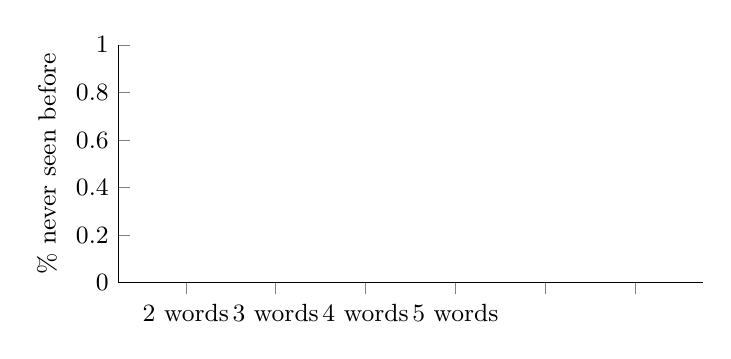
\begin{tikzpicture}
\begin{axis}[ybar, width=9cm, height=4.6cm, bar width=18pt, ymin=0, ymax=110,
  xtick={1,2,3,4,5}, xticklabels={1 word,2 words,3 words,4 words,5 words},
  ylabel={\% never seen before}, ylabel style={font=\small}, tick label style={font=\small},
  nodes near coords, nodes near coords style={font=\footnotesize}, axis lines*=left,
  enlarge x limits=0.15]
\edef\tmp{\noexpand\addplot[fill=black!55, draw=none] coordinates {\cBars};}\tmp
\end{axis}
\end{tikzpicture}
\caption{Sparsity, measured. Sequences in part 9 that never occur in parts 1--8. Single words are
almost always known; by three words, \cUnseenThree\% are new.}
\end{figure}

Single words are almost always known (\cUnseenOne\% unseen). But \cUnseenThree\% of three-word sequences, and
\cUnseenFive\% of five-word sequences, were never seen. And our running phrase? In parts 1--8 the
page \emph{waste of} is completely blank: it occurs \cWasteOfTrain\ times. In part 9 the phrase
\tok{waste of time} occurs \cWasteOfTimeTest\ times. A counting model built from \cTrainWords\ words has nothing
to say about it.

\Sanity Why so empty? With \cVocab\ words there are about \cPossibleTriBillions\ billion possible three-word
sequences; the notebook has seen \cSeenTri\ of them, that is \cTriCoverage\% of the space. More text helps, but
the space grows as $V^n$, much faster than any library.

\Why Clever patches (smoothing, such as Kneser and Ney, 1995) move a little probability onto unseen pages, but
they cannot fix the real problem: \emph{to a counter, every word is a name and nothing more}. Having seen
\emph{waste of money} a thousand times tells it nothing about \emph{waste of time}, because it has no idea that
\emph{money} and \emph{time} are alike.

\begin{wrongidea}{1.5}
\emph{A language model looks up sentences it has already seen.} It was trained on a huge amount of text, so
storing and retrieving sounds plausible. The figure says otherwise: even inside talks on one
topic, most three-word sequences in a new part were never seen before. A model that only looked things up
would be silent most of the time. Whatever a useful model does, it has to work on text it has never seen.
\end{wrongidea}

\begin{wrongidea}{1.8}
\emph{A counting model knows that \emph{time} and \emph{money} are alike.} You know it, and the model has seen
both words many times, so it feels like it should. But the notebook stores counts of exact sequences. Nothing in
it connects the page \emph{waste of money} to the page \emph{waste of time}. That connection is what \S1.5 adds.
\end{wrongidea}

\begin{checkq}
A three-word counting model is built from parts 1--8 and is given \tok{waste of}. What does it predict next?
\begin{options}
\item \tok{time}, because \tok{waste of time} is a common English phrase.
\item Nothing: \tok{waste of} never occurs in those parts, so the count is zero.
\item \tok{time}, because it has seen \tok{waste of money} and knows \emph{money} and \emph{time} are alike.
\item \tok{time}, because \tok{waste of time} occurs \cWasteOfTimeTest\ times in part 9.
\end{options}
\end{checkq}

\begin{sidebar}
\textbf{Requirement 1.} Words must have a notion of \emph{similarity}, so that what is learned about one word
transfers to similar words.
\end{sidebar}

\Summary{Counting what came next fails because almost every sequence is new, and a counter cannot transfer
what it knows to similar words.}

%---------------------------------------------------------------------
\subsection*{1.4\quad Attempt: forget the order, count the words}

A tempting shortcut, long used in search engines and spam filters: throw the words into a bag and only count
them. A bag of \emph{waste}, \emph{of}, \emph{time} is never sparse.

\Predict Do these two customer replies give the same bag of words?
\begin{center}
\tok{not useful, very good} \qquad and \qquad \tok{very useful, not good}
\end{center}
They contain exactly the same words the same number of times, so their bags are identical (our script checks
this). They mean opposite things. Order is not decoration; it carries meaning.

\begin{wrongidea}{1.6}
\emph{If the right words are present, their order hardly matters.} Keyword search works well in daily life, so
this is easy to believe. The pair above has the right words and the opposite meaning. Order matters most for
exactly the small words, like \emph{not}, that the rules of \S1.2 tripped on.
\end{wrongidea}

\begin{checkq}
Which pair of replies would a bag-of-words model treat as identical?
\begin{options}
\item \tok{good, not cheap} and \tok{cheap, not good}
\item \tok{waste of time} and \tok{waste of money}
\item \tok{not useful} and \tok{useless}
\item None: a bag of words keeps the order of the first and last word.
\end{options}
\end{checkq}

\begin{sidebar}
\textbf{Requirement 2.} The model must know \emph{which word came where}.
\end{sidebar}

\Summary{Counting words without their order removes sparsity but also removes meaning, so order must be kept.}

%---------------------------------------------------------------------
\subsection*{1.5\quad Attempt: words as points in space (2003, 2013)}

\Picture Imagine a map of a city where every word lives at an address. \emph{Time} lives next door to
\emph{money} and \emph{effort} (things you can waste); \emph{star} lives across town. If you learn something
about one house, you have learned a little about its neighbours.

\begin{breaks}
A city map has two directions. Real word maps have hundreds, so a word can be near \emph{money} in one
direction (things you spend) and near \emph{clock} in another (things you measure). No flat map can show that.
\end{breaks}

\Exactly In the counting model, each word is effectively a \emph{one-hot} vector: a list of $V$ numbers, all zero
except a single 1 at the word's own position. Any two different one-hot vectors are exactly the same distance
apart ($\sqrt2 \approx \hOneHotDist$), so every word is an equal stranger to every other. Bengio and colleagues
(2003) replaced this with a short learned vector of $d$ numbers per word, an \emph{embedding}, and trained a
small neural network to predict the next word from the embeddings of the previous few. Because similar words
end up with similar vectors, knowledge spreads between them. Mikolov and colleagues' \emph{word2vec} (2013) made
such vectors cheap to learn from billions of words.

\Why This meets Requirement 1, and it gives us the most important idea in these notes: \emph{a word is an arrow
in space, and meaning is direction.} Chapter 2 builds it properly; Chapter 3 uses it on every page. But
Bengio's model still looked at a fixed window of the last few words. What about the word fifty words back?

\Summary{Giving each word a learned position in space lets knowledge spread between similar words, but a fixed
window still cannot reach far back.}

%---------------------------------------------------------------------
\subsection*{1.6\quad Attempt: read word by word, keep a running summary (1990 to 2014)}

\Picture Read a story one word at a time, and after each word update a single sticky note that summarises
everything so far. To guess the next word, look only at the sticky note.

\begin{breaks}
A person can reread the story; this reader cannot. Once a detail is rubbed off the note, it is gone.
\end{breaks}

\Exactly This is the \emph{recurrent neural network} (RNN; Elman, 1990; used as a language model by Mikolov and
colleagues, 2010). It keeps a hidden state $\bm{h}_t$ and updates it with each new word:
\[
\bm{h}_t = f(\bm{h}_{t-1}, \bm{x}_t), \qquad P(w_{t+1}\mid w_{\le t}) = g(\bm{h}_t).
\]
It meets Requirement 2 for free, since the note is written in reading order, and in principle it can remember
forever. In practice it breaks in three ways.

\paragraph{Break (i): one sticky note.} Whatever the sentence (three words or three thousand), it must fit into
the same fixed-size $\bm{h}_t$. Detail is squeezed out.

\paragraph{Break (ii): memories fade or explode.}
\Predict Take a single number carried on the note, and let's assume each update multiplies it by 0.9. How much
of it is left after 50 words? More or less than a quarter?

After 10 words \hFadeTen\ of it is left, after 50 words \hFadeFifty, after 100 words $\hFadeHundred$. If the
factor is 1.1, it grows to \hGrowTen, then \hGrowFifty, then $\hGrowHundred$. Real networks multiply by
matrices, not numbers, but the effect is the same, and it hits learning as hard as remembering: the signal that
should teach the network ``the word fifty steps back mattered'' has to travel back through the same fifty
multiplications (Bengio, Simard and Frasconi, 1994). The LSTM (Hochreiter and Schmidhuber, 1997) added
\emph{gates}, learned switches that let the note keep some numbers untouched, which eased this a lot but did not
remove breaks (i) or (iii).

\paragraph{Break (iii): it cannot be done in parallel.} You cannot write note 1000 before note 999, and you
cannot write 999 before 998. A sentence of \hT\ tokens is \hT\ steps that must happen one after another. A GPU
is a machine with thousands of small workers; give it a chain like this and almost all of them wait.

\begin{sidebar}
\textbf{Requirement 3.} Any word must be able to reach any earlier word \emph{directly}, not through a chain of
summaries.\\
\textbf{Requirement 4.} The work for all positions must be doable \emph{at the same time}.
\end{sidebar}

\begin{checkq}
An RNN carries a signal that is multiplied by 0.9 at every word. Which statement is true?
\begin{options}
\item After 50 words, the signal is about half its size.
\item After 50 words, less than 1\% of the signal is left, and the lesson ``this early word mattered'' fades the same way.
\item An LSTM's gates make the RNN process all words at the same time.
\item The fading only affects remembering, not learning.
\end{options}
\end{checkq}

\Summary{An RNN reads in order, but squeezes everything into one note, lets old signals fade, and cannot work on
all positions at once.}

%---------------------------------------------------------------------
\subsection*{1.7\quad The turn: let the reader look back (2014 to 2017)}

In 2014, neural translation systems (Sutskever, Vinyals and Le; Cho and colleagues) read an English sentence
with one RNN into a single vector and wrote the French with another. Break (i) was plain to see: long sentences
came out worse. Bahdanau, Cho and Bengio (2014) proposed a fix: when writing each French word, let the writer
\emph{look back at every English word} and decide how much each one matters right now. They called these weights
\emph{attention}. Requirement 3 was met. But there was still an RNN underneath, so Requirement 4 was not.

In 2017, Vaswani and colleagues asked: \emph{what if attention is all you need?} Drop the RNN entirely. Let every
word look at every earlier word directly, and do it for all words at once. Figure~\ref{fig:rnn-vs-attn} shows
the difference. Their base translation model trained in about twelve hours on eight GPUs. That architecture is
the \emph{transformer}; GPT (2018), GPT-2 (2019) and every model in Chapter 10 are transformers trained on the
next-word game of \S1.2.

\begin{figure}[h]
\centering
\begin{tikzpicture}[font=\small, w/.style={draw, circle, minimum size=0.8cm, inner sep=0pt, line width=0.7pt}, x=1.2cm]
\begin{scope}
\foreach \i/\t in {1/w_1,2/w_2,3/w_3,4/w_4,5/w_5} \node[w] (r\i) at (1.15*\i,0) {$\t$};
\foreach \i [evaluate=\i as \j using int(\i+1)] in {1,...,4} \draw[-{Stealth}] (r\i) -- (r\j);
\node[align=center] at (3.45,-1.05) {RNN: $w_5$ reaches $w_1$ through 4 hops;\\5 steps, one after another};
\end{scope}
\begin{scope}[xshift=7.6cm]
\foreach \i/\t in {1/w_1,2/w_2,3/w_3,4/w_4,5/w_5} \node[w] (a\i) at (1.15*\i,0) {$\t$};
\foreach \i in {1,...,4} \foreach \j in {2,...,5} {
  \ifnum\i<\j \draw[-{Stealth}, black!70, line width=0.6pt] (a\j) to[bend right=40] (a\i); \fi }
\node[align=center] at (3.45,-1.05) {Attention: every word reaches every earlier\\word in 1 hop; all pairs computed at once};
\end{scope}
\end{tikzpicture}
\caption{The two shapes of computation. For a sentence of \hT\ tokens, the RNN needs \hT\ dependent steps and
\hHops\ hops from last to first; attention computes all \hTT\ pairings in one parallel step and connects any two
words in one hop.}
\label{fig:rnn-vs-attn}
\end{figure}

\begin{wrongidea}{1.7}
\emph{Transformers replaced RNNs mainly because they are more accurate.} Better results are the headline of
every paper, so this is the natural reading. Look at the two breaks the transformer removed: the long chain
between distant words (Requirement 3) and the one-step-at-a-time work (Requirement 4). The second one decided
the history: a model that uses every GPU worker at once can be trained on far more text in the same time, and
the accuracy followed from the scale.
\end{wrongidea}

\begin{center}
\small
\begin{tabular}{@{}l l l@{}}
\toprule
Attempt & What it fixed & Where it broke \\
\midrule
Rules & nothing to learn & endless paraphrases, negation\\
$n$-gram counting (1948 on) & learns from text, no labels & \cUnseenThree\% of 3-word sequences unseen\\
Bag of words & no sparsity & order lost: opposite meanings, same bag\\
Embeddings (2003, 2013) & similarity between words & fixed window of recent words\\
RNN, LSTM (1990, 1997) & order; unlimited history in principle & one note; fading; strictly sequential\\
RNN + attention (2014) & direct look-back & still sequential underneath\\
Transformer (2017) & direct look-back, all at once & \emph{order is lost again}: see \S3.11\\
\bottomrule
\end{tabular}
\end{center}

\Summary{Attention gave every word a direct line to every earlier word, and dropping the RNN let all of that run
at once, which is what made training at scale possible.}

%---------------------------------------------------------------------
\subsection*{1.8\quad A real case: Google Translate, 2016}

For a decade, Google Translate worked phrase by phrase: cut the sentence into short chunks, look each chunk up in
a huge table of translations counted from text, then glue and reorder the pieces. That is the counting notebook
of \S1.3, applied to translation, and it had the same weakness: anything outside a chunk was invisible, so whole
sentences came out stiff. In 2016 Google replaced it with a neural system (Wu and colleagues, 2016): LSTMs that
read the whole sentence, with attention letting the writer look back at every source word. That is \S1.6 plus
\S1.7, about a year before the transformer. A year later the transformer paper reported better translation
quality than such systems at a fraction of the training cost.

Tell me: which of the four requirements does each step in this story meet? The phrase table meets none of 1, 3
and 4. The 2016 system meets 1, 2 and 3. The transformer meets 1, 3 and 4, and loses 2 for a while (Chapter 4).

\Summary{A product used by millions went through the same sequence of fixes as these notes, for the same
reasons.}

%---------------------------------------------------------------------
\subsection*{1.9\quad The whole machine at a glance}

Before we open the box, here is the whole forward pass, the route every batch of text takes from characters to
probabilities. Do not try to understand each stage yet; look at the shape of the road.

\Picture An assembly line. Sentences come in at one end as text. They are cut into pieces (tokens), each piece
gets its starting arrow (embedding), and then the arrows pass through a row of identical workstations. At each
station two things happen: the tokens \emph{talk to each other} (attention), then each token \emph{thinks on its
own} about what it heard (the MLP). At the end of the line, every token's arrow is turned into a guess about the
word that comes after it.

\begin{breaks}
On an assembly line each item passes each station once and the stations never look back. Here every station
sees all the tokens of a sentence together, and what one token becomes depends on the others.
\end{breaks}

\paragraph{Drawing the transformer, block by block.} Here is the whole machine as a frame of empty blocks.
Every chapter from now on fills in one or two of them, and opens with this same picture, so you always know
where you are: solid blocks are built, the highlighted block is the one that chapter builds, and dashed blocks
are still ahead. For now only the top is filled in: text comes in.

\machine{1}{The frame we will fill. Text enters at the top; each dashed block is one chapter's job. The middle
part, inside the large rounded box, is one \emph{layer}; a real model stacks $L$ of them. At the bottom, the
model gives a score to every word it knows, of shape $B\times T\times V$: a guess at \emph{every} position of
\emph{every} sentence in one pass, not only at the last one.}

\begin{center}% AUTO-GENERATED by code/figlib.py helpers -- do not edit
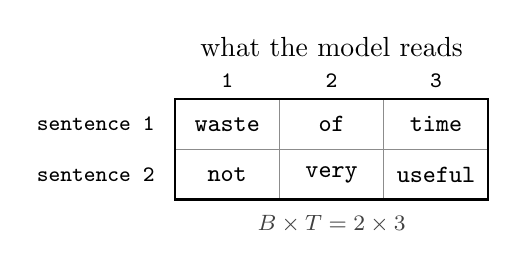
\begin{tikzpicture}[x=1.7cm]
\draw[black!45, fill=white] (0.000,0.000) rectangle (0.780,-0.640);
\node[font=\small, text=black] at (0.390,-0.320) {\texttt{waste}};
\draw[black!45, fill=white] (0.780,0.000) rectangle (1.560,-0.640);
\node[font=\small, text=black] at (1.170,-0.320) {\texttt{of}};
\draw[black!45, fill=white] (1.560,0.000) rectangle (2.340,-0.640);
\node[font=\small, text=black] at (1.950,-0.320) {\texttt{time}};
\draw[black!45, fill=white] (0.000,-0.640) rectangle (0.780,-1.279);
\node[font=\small, text=black] at (0.390,-0.959) {\texttt{not}};
\draw[black!45, fill=white] (0.780,-0.640) rectangle (1.560,-1.279);
\node[font=\small, text=black] at (1.170,-0.959) {\texttt{very}};
\draw[black!45, fill=white] (1.560,-0.640) rectangle (2.340,-1.279);
\node[font=\small, text=black] at (1.950,-0.959) {\texttt{useful}};
\draw[line width=0.9pt] (0.000,0.000) rectangle (2.340,-1.279);
\node[anchor=east, font=\footnotesize\ttfamily] at (-0.080,-0.320) {sentence 1};
\node[anchor=east, font=\footnotesize\ttfamily] at (-0.080,-0.959) {sentence 2};
\node[anchor=south, font=\footnotesize\ttfamily] at (0.390,0.020) {1};
\node[anchor=south, font=\footnotesize\ttfamily] at (1.170,0.020) {2};
\node[anchor=south, font=\footnotesize\ttfamily] at (1.950,0.020) {3};
\node[anchor=south, font=\normalsize] at (1.170,0.420) {what the model reads};
\node[anchor=north, font=\footnotesize, text=black!75] at (1.170,-1.359) {$B\times T=2\times3$};
\end{tikzpicture}
\qquad
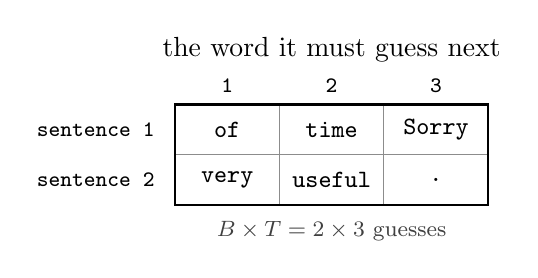
\begin{tikzpicture}[x=1.7cm]
\draw[black!45, fill=white] (0.000,0.000) rectangle (0.780,-0.640);
\node[font=\small, text=black] at (0.390,-0.320) {\texttt{of}};
\draw[black!45, fill=white] (0.780,0.000) rectangle (1.560,-0.640);
\node[font=\small, text=black] at (1.170,-0.320) {\texttt{time}};
\draw[black!45, fill=white] (1.560,0.000) rectangle (2.340,-0.640);
\node[font=\small, text=black] at (1.950,-0.320) {\texttt{Sorry}};
\draw[black!45, fill=white] (0.000,-0.640) rectangle (0.780,-1.279);
\node[font=\small, text=black] at (0.390,-0.959) {\texttt{very}};
\draw[black!45, fill=white] (0.780,-0.640) rectangle (1.560,-1.279);
\node[font=\small, text=black] at (1.170,-0.959) {\texttt{useful}};
\draw[black!45, fill=white] (1.560,-0.640) rectangle (2.340,-1.279);
\node[font=\small, text=black] at (1.950,-0.959) {\texttt{.}};
\draw[line width=0.9pt] (0.000,0.000) rectangle (2.340,-1.279);
\node[anchor=east, font=\footnotesize\ttfamily] at (-0.080,-0.320) {sentence 1};
\node[anchor=east, font=\footnotesize\ttfamily] at (-0.080,-0.959) {sentence 2};
\node[anchor=south, font=\footnotesize\ttfamily] at (0.390,0.020) {1};
\node[anchor=south, font=\footnotesize\ttfamily] at (1.170,0.020) {2};
\node[anchor=south, font=\footnotesize\ttfamily] at (1.950,0.020) {3};
\node[anchor=south, font=\normalsize] at (1.170,0.420) {the word it must guess next};
\node[anchor=north, font=\footnotesize, text=black!75] at (1.170,-1.359) {$B\times T=2\times3$ guesses};
\end{tikzpicture}
\end{center}

Look at the two tables above. That is the quiet reason transformers train so fast. A sentence of $T$ tokens is not one exercise
but $T$ exercises: after \tok{waste}, guess \tok{of}; after \tok{waste of}, guess \tok{time}; after \tok{waste
of time}, guess \tok{Sorry}. The transformer answers all of them in the same pass, for all $B$ sentences in the
batch. How can it do that without cheating, without the guess for position 2 peeking at the answer in position
3? That is one of the things Chapter 3 has to explain.

\begin{checkq}
A batch holds $B=8$ sentences of $T=16$ tokens each. How many next-word guesses does one forward pass produce?
\begin{options}
\item 8, one per sentence.
\item 16, one per position.
\item 128, one per position of every sentence.
\item It depends on how long the reply is.
\end{options}
\end{checkq}

\Summary{One pass turns $B$ sentences of $T$ tokens into $B\times T$ next-word guesses, through tokens,
embeddings, $L$ talk-then-think stations and a final scoring step.}

%---------------------------------------------------------------------
\begin{lookingback}
These look back at Chapter 0, the notation page.
(1) What do $B$, $T$ and $d$ stand for, in words? (2) A matrix has shape $3\times4$. How many rows does it have,
and what does each row hold in these notes? (3) Which symbol will stand for the number of learned parameters?
\end{lookingback}

\subsection*{Exercises}

\begin{exercise}
A notebook model looks at the previous 4 words, and the vocabulary has 50{,}000 words. How many pages could the
notebook have? Is that more or less than the number of words ever written?
\end{exercise}

\begin{exercise}
Using the bag-of-words idea, find two more replies a support team might receive that have identical bags but
opposite meanings.
\end{exercise}

\begin{exercise}
An RNN multiplies a signal by 0.95 per word. After how many words is less than 1\% of it left?
\end{exercise}

\begin{exercise}
Write the chain rule for the reply \tok{Sorry , this has not been useful} given \tok{waste of time}: how many
factors are there, and what does the third factor condition on?
\end{exercise}

\subsection*{Answers to Chapter 1}
\small
\textbf{Check yourself 1.1.} (b). A chain of guesses multiplies, so the whole is less likely than each part:
$0.95^{10}\approx\nOneTenRight$. (a) treats the whole reply as one guess. (c) is the wrong idea M1.3: wrong words come
from the guessing process itself. (d) is M1.2: ``I am 95\% sure'' is more text, not a measurement.

\textbf{Check yourself 1.2.} (b). The page \emph{waste of} is blank: \cWasteOfTrain\ occurrences. (a) is M1.5:
the model does not look things up in ``English''; it only has its notebook. (c) is M1.8: counts do not know
which words are alike. (d) uses data the model never trained on, the same leakage your fraud model must avoid.

\textbf{Check yourself 1.3.} (a). Same words, same counts, opposite meanings. (b) differ in one word. (c) have
different words. (d) is M1.6 in disguise: a bag keeps no order at all.

\textbf{Check yourself 1.4.} (b). $0.9^{50}=\hFadeFifty$. (a) underestimates how fast repeated multiplication
shrinks a number. (c) is wrong: gates help memory, not parallelism (M1.7 is the belief that accuracy, not
parallelism, was the deciding issue). (d) misses that learning signals travel back through the same steps.

\textbf{Check yourself 1.5.} (c). $8\times16=128$: every position of every sentence predicts its next token. (a)
and (b) count one dimension only. (d) confuses training on given text with writing a new reply.

\textbf{Looking back.} (1) Batch size, tokens per sentence, numbers per token. (2) Three rows, one per token.
(3) $N$.

\textbf{Exercise 1.1.} $50{,}000^4 = \hExPages$ possible four-word contexts; far more than all words ever
written, so almost every page stays empty.

\textbf{Exercise 1.2.} For example \tok{good, not cheap} (good but expensive) versus \tok{cheap, not good}.

\textbf{Exercise 1.3.} We need $0.95^n < 0.01$, that is $n > \ln 0.01/\ln 0.95 \approx \hExN$, so after
\hExNceil\ words.

\textbf{Exercise 1.4.} Seven factors, one per reply token. The third is $P(\tok{this}\mid\tok{waste of time Sorry ,})$:
it conditions on the message and the two reply tokens before it.
\normalsize

\subsection*{What you now know}
\begin{itemize}
\item Why writing a reply one word at a time beats rules and fixed reply lists, and why that game labels itself.
\item How the chain rule turns a sentence into a product of next-word probabilities, and why errors compound.
\item Why counting, bag of words, word vectors, RNNs and RNN-plus-attention each fell short, measured where
possible, and the four requirements those failures left behind.
\item The shape of the whole forward pass, and why one pass gives $B\times T$ guesses.
\end{itemize}

\clearpage\newpage
\section*{2\quad Tokens, and words as points in space}
\addcontentsline{toc}{section}{2 Tokens, and words as points in space}
\startchapter{2}

\begin{chaptermap}
A model cannot read. It receives numbers. This chapter answers two questions: how do we cut text into
pieces the model can count (\emph{tokens}), and how does each piece become an arrow of $d$ numbers
(an \emph{embedding})? We try whole words, then single letters, watch both break on real text, and arrive
at byte-pair encoding. Then we turn each token into an arrow, first by plain lookup and then by asking
where good arrows come from. It ends with Requirement 1 of Chapter 1 met: similar words sit near each
other, and Chapter 3 can start moving them.
\end{chaptermap}

\machine{2}{You are here: Chapter 2 builds the first two blocks, cutting text into tokens and looking up one arrow per token. Every later block works on these arrows.}

\begin{beforeyoustart}
(1) In a list of 1000 words, 25 have never been seen before. What percentage is that?
(2) Count the pairs of letters in the word \tok{banana}, reading left to right. How many times does
\tok{an} appear? (3) A table has 12 rows and 4 columns. How many numbers does it hold?
(4) If two arrows point at right angles, what is their dot product?

\smallskip\noindent\textit{Refreshers.} (1) $25/1000 = 0.025$, which is 2.5\%. (2) The pairs are \tok{ba},
\tok{an}, \tok{na}, \tok{an}, \tok{na}: \tok{an} appears twice. Overlapping pairs count separately.
(3) $12\times4=48$. (4) Zero (Chapter 3, \S3.2): no shadow, nothing in common.
\end{beforeyoustart}

%---------------------------------------------------------------------
\subsection*{2.1\quad What does the model receive?}

\Predict When you type \tok{waste of time} into a chat model, what arrives at the first layer of the
model: letters, words, or something else? Write your guess down before reading on.

The answer is a short list of whole numbers, one per piece of text, such as $(\nTwoTimeId)$ for the
toy word \tok{time}. Everything the model will ever know about your message has to travel through those
numbers. So the first design decision in any language model is a quiet one: \emph{what counts as one
piece?} Let us try the two obvious answers and watch them break, with numbers from the same corpus as
Chapter 1: transcribed technical talks on AI engineering, split into nine parts.

\Summary{the model never sees text, only a list of token numbers, so we must decide what one token is.}

%---------------------------------------------------------------------
\subsection*{2.2\quad Two simple choices, and how each breaks}

\paragraph{Choice 1: one token per word.} This is how you read, so it feels natural. In parts 1--8 there
are \cTrainWords\ words but only \nTwoWordVocab\ different ones, so the table of words is small.

\paragraph{How it breaks.} Language keeps inventing words. In part 9, \nTwoUnseenWordPct\% of the
words (\nTwoUnseenTypes\ different ones) never appeared in parts 1--8, and a word-level model has no
row for any of them. What would you do with a word you have no row for? Use the nearest known word? Split it
into smaller pieces? Write it down as ``unknown''? All three are reasonable guesses.

Older systems did the last one: every new word became one special token, \tok{<unk>}, and all of them
looked the same to the model. A customer who writes a product name the model has never seen would be
answered as if they had written nothing. And the long tail is not small: \nTwoSingletonPct\% of the
different words in parts 1--8 (\nTwoSingletons\ of them) appear exactly once.

\paragraph{Choice 2: one token per letter.} There are only \nTwoChars\ different letters in the
corpus, so nothing is ever unknown.

\paragraph{How it breaks.} The text gets long. An average word here is \nTwoCharsPerWord\ letters, plus a
marker for the end of the word, about \nTwoTpwZero\ tokens per word. Chapter 3 compares every token with
every earlier token, so the work grows with the \emph{square} of the length: roughly $\nTwoTpwZero^2
\approx \nTwoPairFactor$ times more comparisons than one token per word. And a single letter carries
almost no meaning, so the model must spend layers re-assembling words before it can think about them.

\begin{checkq}
You are building a model for a support team whose customers often type new product names. Which choice
breaks for them first, and why?
\begin{options}
\item One token per word, because every new product name has no row in the table.
\item One token per letter, because product names are long.
\item Neither, because the model reads the name the way a person does.
\item One token per word, because product names are longer than other words.
\end{options}
\end{checkq}

\Summary{whole words leave new words with nowhere to go; single letters make every sentence about five
times longer and attention about \nTwoPairFactor\ times more expensive.}

%---------------------------------------------------------------------
\subsection*{2.3\quad The middle path: byte-pair encoding}

\Predict Suppose you could give a few hundred common letter-groups their own token, and spell everything
else out of letters. Which groups would you pick first?

\Picture Think about how people take fast notes. Nobody invents a shorthand for a word used once, but a
phrase you write twenty times in a meeting soon gets an abbreviation. Byte-pair encoding does exactly
that, automatically: it looks for the pair of symbols that sits side by side most often in the text, and
gives that pair its own symbol. Then it does it again, and again.

\paragraph{The numbers.} We ran it from scratch on parts 1--8 (the script is \texttt{code/ch2\_bpe.py}).
Each word starts as its letters followed by an end-of-word marker \tok{\_}, so the word \tok{time}
starts as \nTwoSegZeroTime. The first merges, with how often each pair appeared:

\begin{center}
\small
\begin{tabular}{@{}r l r@{\qquad}r l r@{}}
\toprule
merge & pair & times seen & merge & pair & times seen\\
\midrule
1 & \nTwoMergeOne & \nTwoMergeCountOne & 5 & \nTwoMergeFive & \nTwoMergeCountFive\\
2 & \nTwoMergeTwo & \nTwoMergeCountTwo & 6 & \nTwoMergeSix & \nTwoMergeCountSix\\
3 & \nTwoMergeThree & \nTwoMergeCountThree & 7 & \nTwoMergeSeven & \nTwoMergeCountSeven\\
4 & \nTwoMergeFour & \nTwoMergeCountFour & 8 & \nTwoMergeEight & \nTwoMergeCountEight\\
\bottomrule
\end{tabular}
\end{center}

\noindent Did your prediction include \tok{e\_}, a word ending in ``e''? Very few people guess it, and it
is the most common pair of all. After \nTwoMerges\ merges the vocabulary has \nTwoBpeVocab\ symbols, and
our running words split like this:

\begin{center}
\small
\begin{tabular}{@{}l l l l@{}}
\toprule
word & 0 merges & 100 merges & \nTwoMerges\ merges\\
\midrule
\tok{waste} & \nTwoSegZeroWaste & \nTwoSegHundredWaste & \nTwoSegWaste\\
\tok{of} & \nTwoSegZeroOf & \nTwoSegHundredOf & \nTwoSegOf\\
\tok{time} & \nTwoSegZeroTime & \nTwoSegHundredTime & \nTwoSegTime\\
\bottomrule
\end{tabular}
\end{center}

Common words become one token. Rarer words become a few familiar pieces. And now the real test: the word
\tok{\nTwoUnseenWord} appears \nTwoUnseenWordCount\ times in part 9 and never in parts 1--8. A
word-level model would have nothing. Byte-pair encoding writes it as \nTwoSegUnseen. Of the
\nTwoTestWords\ words in part 9, the number that cannot be written at all is \nTwoUnkAfter, and the
average word costs \nTwoTokPerWord\ tokens, against \nTwoTpwZero\ for single letters.

\begin{figure}[h]
\centering
\begin{tikzpicture}
\begin{axis}[width=8.5cm, height=4.6cm, xlabel={vocabulary size (symbols)}, ylabel={tokens per word},
  xlabel style={font=\small}, ylabel style={font=\small}, tick label style={font=\small},
  axis lines*=left, mark size=1.6pt, ymin=1, ymax=5.6,
  nodes near coords, point meta=explicit symbolic, nodes near coords style={font=\footnotesize, anchor=south west}]
\addplot[black, mark=*] table[x=vocab, y=tpw, meta=merges] {data_ch2/bpe_growth.dat};
\end{axis}
\end{tikzpicture}
\caption{Measured on part 9: the more merges (numbers on the points), the fewer tokens each word costs.
The curve flattens, so the vocabulary size is a trade-off between table size and sequence length.}
\end{figure}

\Exactly Byte-pair encoding (Gage, 1994, as a compression method; Sennrich, Haddow and Birch, 2016, for
translation) builds the vocabulary in a loop:
\begin{enumerate}[label=\arabic*.]
\item Start with every word written as single symbols plus an end marker. The vocabulary is the set of
single symbols.
\item Count every pair of neighbouring symbols across the whole text, weighted by how often each word appears.
\item Add the most frequent pair to the vocabulary as one new symbol, and rewrite the text with it.
\item Repeat until the vocabulary has the size you chose.
\end{enumerate}
To cut new text into tokens, apply the learned merges in the order they were learned. GPT-2 (Radford
and colleagues, 2019) starts from the 256 possible \emph{bytes} instead of letters, so any text in any
language, including emoji and code, can always be written. Real tokenizers are this same loop run on far
more text: Qwen3 uses a vocabulary of 151{,}936 entries, as published in the Qwen3 technical report (2025;
we will check this against the model's \texttt{config.json} in Chapter 10). The tokenizer's own list
is slightly shorter, 151{,}669 entries; the embedding table is padded to a slightly larger size.

\begin{breaks}
Shorthand notes are written by one person for a reason they understand. Byte-pair encoding has no idea
what a pair means; it only counts. So \tok{e\_} becomes a token because it is frequent, not because it is a
unit of meaning. The model has to learn meaning later.
\end{breaks}

\Why Two pressures pull in opposite directions: a small vocabulary keeps the table small and leaves no word
unknown; a large vocabulary keeps sequences short. Frequency is a fair referee between them, because the
things you write often are the things worth a dedicated symbol.

\begin{wrongidea}{2.2}
``A word the model has never seen makes it fail or print \emph{unknown}.'' With byte-pair encoding there is
always a way to spell the word, down to single letters or bytes. The model never fails to \emph{read} a new
word. Whether it \emph{understands} it is a separate question: \tok{\nTwoUnseenWord} arrives as pieces, and
the model has to build the meaning from \tok{ok}, \tok{en}, \tok{iz}, \tok{er\_} and the words around them.
\end{wrongidea}

\begin{wrongidea}{2.3}
``A token is a word.'' It is tempting because for common words like \tok{of} and \tok{time} it is
true. But \tok{waste} became three tokens in our tokenizer. Measured on part 9, one of our tokens is on average \nTwoWordsPerTok\ of a word, and a rare word is
several tokens.
\end{wrongidea}

\begin{checkq}
After \nTwoMerges\ merges, \tok{time} is one token but \tok{waste} is three. What best explains this?
\begin{options}
\item \tok{time} is more important for meaning than \tok{waste}.
\item In parts 1--8, the pieces of \tok{time} were merged often enough to become one symbol, and
\tok{waste} was rarer.
\item The tokenizer splits every word into its syllables.
\item \tok{waste} has more letters, and long words are always split.
\end{options}
\end{checkq}

\Summary{byte-pair encoding gives frequent letter-groups their own token and spells everything else from
smaller pieces, so nothing is ever unknown and common words stay short.}

%---------------------------------------------------------------------
\subsection*{2.4\quad From a token number to an arrow: the embedding table}

\Predict The token \tok{time} is number \nTwoTimeId\ in our toy vocabulary and \tok{of} is number 1. Does
that mean \tok{time} and \tok{of} are similar, because 1 and \nTwoTimeId\ are close?

\Picture A token number is a locker number. Locker 2 is next to locker 1, but that tells you nothing
about what is inside. To get the contents you walk to the locker and open it. The embedding table is the
row of lockers, and each locker holds an arrow of $d$ numbers.

\paragraph{The numbers.} Our toy model knows \nTwoVocabSize\ tokens, each with an arrow of $d=4$ numbers.
First, the text becomes token numbers, one per token; a batch of sentences becomes a table of numbers:
\begin{center}% AUTO-GENERATED by code/figlib.py helpers -- do not edit
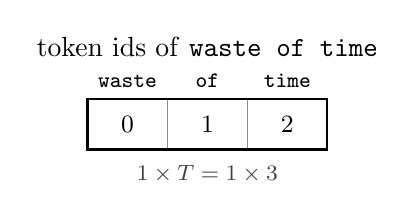
\begin{tikzpicture}[x=1.3cm]
\draw[black!45, fill=white] (0.000,0.000) rectangle (0.780,-0.640);
\node[font=\small, text=black] at (0.390,-0.320) {$0$};
\draw[black!45, fill=white] (0.780,0.000) rectangle (1.560,-0.640);
\node[font=\small, text=black] at (1.170,-0.320) {$1$};
\draw[black!45, fill=white] (1.560,0.000) rectangle (2.340,-0.640);
\node[font=\small, text=black] at (1.950,-0.320) {$2$};
\draw[line width=0.9pt] (0.000,0.000) rectangle (2.340,-0.640);
\node[anchor=south, font=\footnotesize\ttfamily] at (0.390,0.020) {waste};
\node[anchor=south, font=\footnotesize\ttfamily] at (1.170,0.020) {of};
\node[anchor=south, font=\footnotesize\ttfamily] at (1.950,0.020) {time};
\node[anchor=south, font=\normalsize] at (1.170,0.420) {token ids of \texttt{waste of time}};
\node[anchor=north, font=\footnotesize, text=black!75] at (1.170,-0.720) {$1\times T=1\times3$};
\end{tikzpicture}
\qquad\qquad
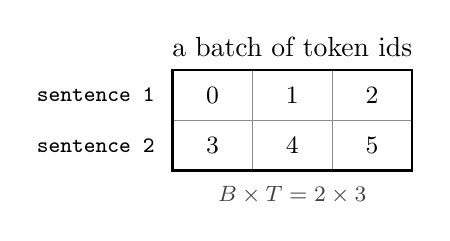
\begin{tikzpicture}[x=1.3cm]
\draw[black!45, fill=white] (0.000,0.000) rectangle (0.780,-0.640);
\node[font=\small, text=black] at (0.390,-0.320) {$0$};
\draw[black!45, fill=white] (0.780,0.000) rectangle (1.560,-0.640);
\node[font=\small, text=black] at (1.170,-0.320) {$1$};
\draw[black!45, fill=white] (1.560,0.000) rectangle (2.340,-0.640);
\node[font=\small, text=black] at (1.950,-0.320) {$2$};
\draw[black!45, fill=white] (0.000,-0.640) rectangle (0.780,-1.279);
\node[font=\small, text=black] at (0.390,-0.959) {$3$};
\draw[black!45, fill=white] (0.780,-0.640) rectangle (1.560,-1.279);
\node[font=\small, text=black] at (1.170,-0.959) {$4$};
\draw[black!45, fill=white] (1.560,-0.640) rectangle (2.340,-1.279);
\node[font=\small, text=black] at (1.950,-0.959) {$5$};
\draw[line width=0.9pt] (0.000,0.000) rectangle (2.340,-1.279);
\node[anchor=east, font=\footnotesize\ttfamily] at (-0.080,-0.320) {sentence 1};
\node[anchor=east, font=\footnotesize\ttfamily] at (-0.080,-0.959) {sentence 2};
\node[anchor=south, font=\normalsize] at (1.170,0.050) {a batch of token ids};
\node[anchor=north, font=\footnotesize, text=black!75] at (1.170,-1.359) {$B\times T=2\times3$};
\end{tikzpicture}
\end{center}
Each number opens one row of the embedding table $E$. Rows 0--2 are the arrows Chapter 3 uses; the
highlighted row is \tok{time}:
\begin{center}% AUTO-GENERATED by code/figlib.py helpers -- do not edit
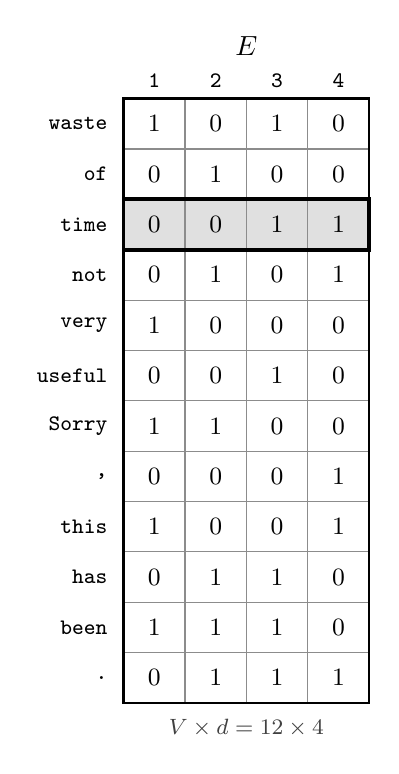
\begin{tikzpicture}
\draw[black!45, fill=white] (0.000,0.000) rectangle (0.780,-0.640);
\node[font=\small, text=black] at (0.390,-0.320) {$1$};
\draw[black!45, fill=white] (0.780,0.000) rectangle (1.560,-0.640);
\node[font=\small, text=black] at (1.170,-0.320) {$0$};
\draw[black!45, fill=white] (1.560,0.000) rectangle (2.340,-0.640);
\node[font=\small, text=black] at (1.950,-0.320) {$1$};
\draw[black!45, fill=white] (2.340,0.000) rectangle (3.120,-0.640);
\node[font=\small, text=black] at (2.730,-0.320) {$0$};
\draw[black!45, fill=white] (0.000,-0.640) rectangle (0.780,-1.279);
\node[font=\small, text=black] at (0.390,-0.959) {$0$};
\draw[black!45, fill=white] (0.780,-0.640) rectangle (1.560,-1.279);
\node[font=\small, text=black] at (1.170,-0.959) {$1$};
\draw[black!45, fill=white] (1.560,-0.640) rectangle (2.340,-1.279);
\node[font=\small, text=black] at (1.950,-0.959) {$0$};
\draw[black!45, fill=white] (2.340,-0.640) rectangle (3.120,-1.279);
\node[font=\small, text=black] at (2.730,-0.959) {$0$};
\draw[black!45, fill=black!12] (0.000,-1.279) rectangle (0.780,-1.919);
\node[font=\small, text=black] at (0.390,-1.599) {$0$};
\draw[black!45, fill=black!12] (0.780,-1.279) rectangle (1.560,-1.919);
\node[font=\small, text=black] at (1.170,-1.599) {$0$};
\draw[black!45, fill=black!12] (1.560,-1.279) rectangle (2.340,-1.919);
\node[font=\small, text=black] at (1.950,-1.599) {$1$};
\draw[black!45, fill=black!12] (2.340,-1.279) rectangle (3.120,-1.919);
\node[font=\small, text=black] at (2.730,-1.599) {$1$};
\draw[black!45, fill=white] (0.000,-1.919) rectangle (0.780,-2.558);
\node[font=\small, text=black] at (0.390,-2.239) {$0$};
\draw[black!45, fill=white] (0.780,-1.919) rectangle (1.560,-2.558);
\node[font=\small, text=black] at (1.170,-2.239) {$1$};
\draw[black!45, fill=white] (1.560,-1.919) rectangle (2.340,-2.558);
\node[font=\small, text=black] at (1.950,-2.239) {$0$};
\draw[black!45, fill=white] (2.340,-1.919) rectangle (3.120,-2.558);
\node[font=\small, text=black] at (2.730,-2.239) {$1$};
\draw[black!45, fill=white] (0.000,-2.558) rectangle (0.780,-3.198);
\node[font=\small, text=black] at (0.390,-2.878) {$1$};
\draw[black!45, fill=white] (0.780,-2.558) rectangle (1.560,-3.198);
\node[font=\small, text=black] at (1.170,-2.878) {$0$};
\draw[black!45, fill=white] (1.560,-2.558) rectangle (2.340,-3.198);
\node[font=\small, text=black] at (1.950,-2.878) {$0$};
\draw[black!45, fill=white] (2.340,-2.558) rectangle (3.120,-3.198);
\node[font=\small, text=black] at (2.730,-2.878) {$0$};
\draw[black!45, fill=white] (0.000,-3.198) rectangle (0.780,-3.838);
\node[font=\small, text=black] at (0.390,-3.518) {$0$};
\draw[black!45, fill=white] (0.780,-3.198) rectangle (1.560,-3.838);
\node[font=\small, text=black] at (1.170,-3.518) {$0$};
\draw[black!45, fill=white] (1.560,-3.198) rectangle (2.340,-3.838);
\node[font=\small, text=black] at (1.950,-3.518) {$1$};
\draw[black!45, fill=white] (2.340,-3.198) rectangle (3.120,-3.838);
\node[font=\small, text=black] at (2.730,-3.518) {$0$};
\draw[black!45, fill=white] (0.000,-3.838) rectangle (0.780,-4.477);
\node[font=\small, text=black] at (0.390,-4.157) {$1$};
\draw[black!45, fill=white] (0.780,-3.838) rectangle (1.560,-4.477);
\node[font=\small, text=black] at (1.170,-4.157) {$1$};
\draw[black!45, fill=white] (1.560,-3.838) rectangle (2.340,-4.477);
\node[font=\small, text=black] at (1.950,-4.157) {$0$};
\draw[black!45, fill=white] (2.340,-3.838) rectangle (3.120,-4.477);
\node[font=\small, text=black] at (2.730,-4.157) {$0$};
\draw[black!45, fill=white] (0.000,-4.477) rectangle (0.780,-5.117);
\node[font=\small, text=black] at (0.390,-4.797) {$0$};
\draw[black!45, fill=white] (0.780,-4.477) rectangle (1.560,-5.117);
\node[font=\small, text=black] at (1.170,-4.797) {$0$};
\draw[black!45, fill=white] (1.560,-4.477) rectangle (2.340,-5.117);
\node[font=\small, text=black] at (1.950,-4.797) {$0$};
\draw[black!45, fill=white] (2.340,-4.477) rectangle (3.120,-5.117);
\node[font=\small, text=black] at (2.730,-4.797) {$1$};
\draw[black!45, fill=white] (0.000,-5.117) rectangle (0.780,-5.756);
\node[font=\small, text=black] at (0.390,-5.437) {$1$};
\draw[black!45, fill=white] (0.780,-5.117) rectangle (1.560,-5.756);
\node[font=\small, text=black] at (1.170,-5.437) {$0$};
\draw[black!45, fill=white] (1.560,-5.117) rectangle (2.340,-5.756);
\node[font=\small, text=black] at (1.950,-5.437) {$0$};
\draw[black!45, fill=white] (2.340,-5.117) rectangle (3.120,-5.756);
\node[font=\small, text=black] at (2.730,-5.437) {$1$};
\draw[black!45, fill=white] (0.000,-5.756) rectangle (0.780,-6.396);
\node[font=\small, text=black] at (0.390,-6.076) {$0$};
\draw[black!45, fill=white] (0.780,-5.756) rectangle (1.560,-6.396);
\node[font=\small, text=black] at (1.170,-6.076) {$1$};
\draw[black!45, fill=white] (1.560,-5.756) rectangle (2.340,-6.396);
\node[font=\small, text=black] at (1.950,-6.076) {$1$};
\draw[black!45, fill=white] (2.340,-5.756) rectangle (3.120,-6.396);
\node[font=\small, text=black] at (2.730,-6.076) {$0$};
\draw[black!45, fill=white] (0.000,-6.396) rectangle (0.780,-7.036);
\node[font=\small, text=black] at (0.390,-6.716) {$1$};
\draw[black!45, fill=white] (0.780,-6.396) rectangle (1.560,-7.036);
\node[font=\small, text=black] at (1.170,-6.716) {$1$};
\draw[black!45, fill=white] (1.560,-6.396) rectangle (2.340,-7.036);
\node[font=\small, text=black] at (1.950,-6.716) {$1$};
\draw[black!45, fill=white] (2.340,-6.396) rectangle (3.120,-7.036);
\node[font=\small, text=black] at (2.730,-6.716) {$0$};
\draw[black!45, fill=white] (0.000,-7.036) rectangle (0.780,-7.675);
\node[font=\small, text=black] at (0.390,-7.355) {$0$};
\draw[black!45, fill=white] (0.780,-7.036) rectangle (1.560,-7.675);
\node[font=\small, text=black] at (1.170,-7.355) {$1$};
\draw[black!45, fill=white] (1.560,-7.036) rectangle (2.340,-7.675);
\node[font=\small, text=black] at (1.950,-7.355) {$1$};
\draw[black!45, fill=white] (2.340,-7.036) rectangle (3.120,-7.675);
\node[font=\small, text=black] at (2.730,-7.355) {$1$};
\draw[line width=1.4pt] (0.000,-1.279) rectangle (3.120,-1.919);
\draw[line width=0.9pt] (0.000,0.000) rectangle (3.120,-7.675);
\node[anchor=east, font=\footnotesize\ttfamily] at (-0.080,-0.320) {waste};
\node[anchor=east, font=\footnotesize\ttfamily] at (-0.080,-0.959) {of};
\node[anchor=east, font=\footnotesize\ttfamily] at (-0.080,-1.599) {time};
\node[anchor=east, font=\footnotesize\ttfamily] at (-0.080,-2.239) {not};
\node[anchor=east, font=\footnotesize\ttfamily] at (-0.080,-2.878) {very};
\node[anchor=east, font=\footnotesize\ttfamily] at (-0.080,-3.518) {useful};
\node[anchor=east, font=\footnotesize\ttfamily] at (-0.080,-4.157) {Sorry};
\node[anchor=east, font=\footnotesize\ttfamily] at (-0.080,-4.797) {,};
\node[anchor=east, font=\footnotesize\ttfamily] at (-0.080,-5.437) {this};
\node[anchor=east, font=\footnotesize\ttfamily] at (-0.080,-6.076) {has};
\node[anchor=east, font=\footnotesize\ttfamily] at (-0.080,-6.716) {been};
\node[anchor=east, font=\footnotesize\ttfamily] at (-0.080,-7.355) {.};
\node[anchor=south, font=\footnotesize\ttfamily] at (0.390,0.020) {1};
\node[anchor=south, font=\footnotesize\ttfamily] at (1.170,0.020) {2};
\node[anchor=south, font=\footnotesize\ttfamily] at (1.950,0.020) {3};
\node[anchor=south, font=\footnotesize\ttfamily] at (2.730,0.020) {4};
\node[anchor=south, font=\normalsize] at (1.560,0.420) {$E$};
\node[anchor=north, font=\footnotesize, text=black!75] at (1.560,-7.755) {$V\times d=12\times4$};
\end{tikzpicture}
\end{center}
To fetch \tok{time} with a multiplication, write its number as a \emph{one-hot} row: twelve zeros with a
single 1 in position \nTwoTimeId\ (counting from 0). Multiplying that row by $E$ picks out exactly one row,
because every other row is multiplied by 0:
\begin{figure}[!htb]\centering
\resizebox{\linewidth}{!}{% AUTO-GENERATED by code/figlib.py helpers -- do not edit
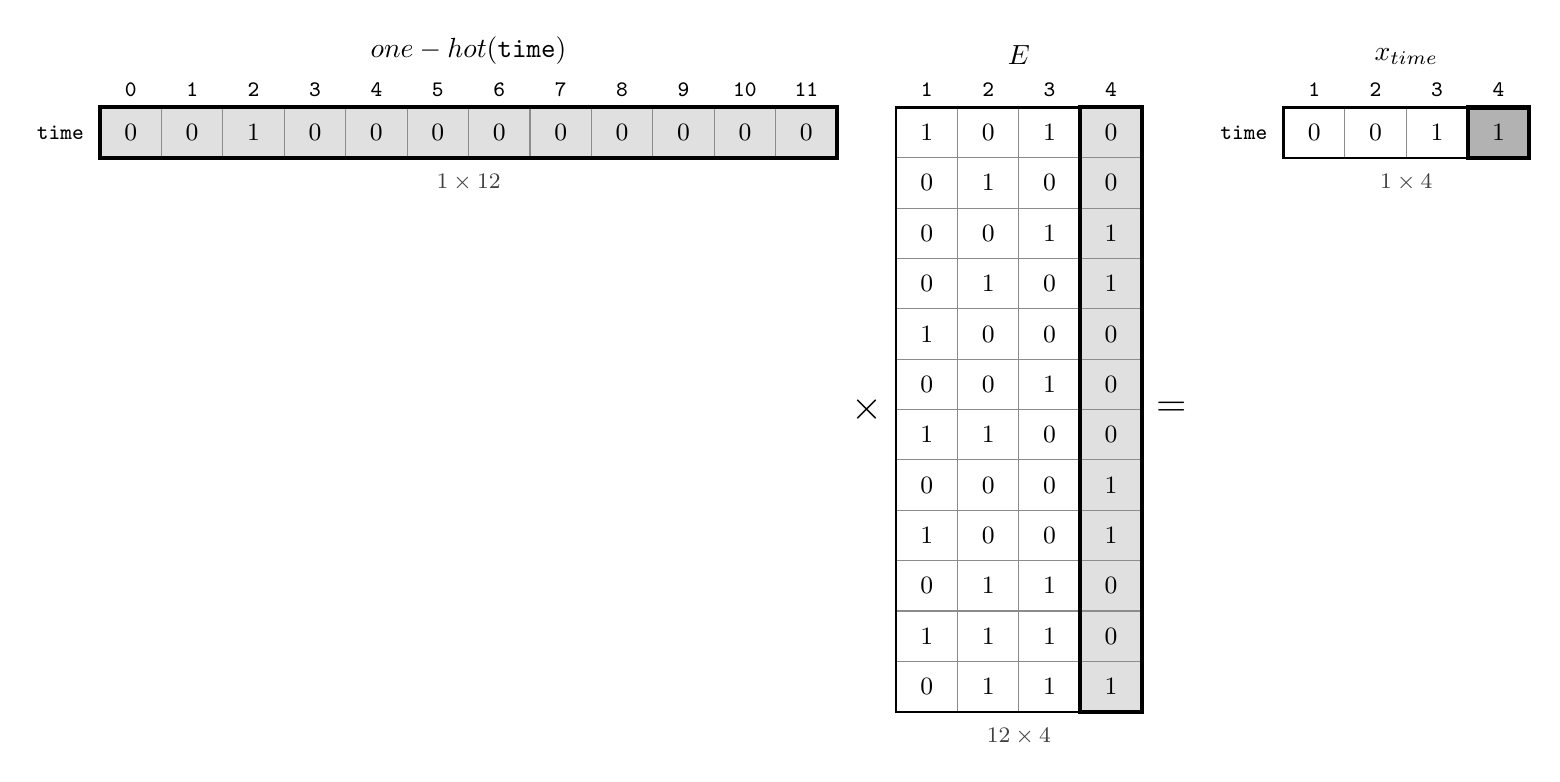
\begin{tikzpicture}
\draw[black!45, fill=black!12] (0.000,0.000) rectangle (0.780,-0.640);
\node[font=\small, text=black] at (0.390,-0.320) {$0$};
\draw[black!45, fill=black!12] (0.780,0.000) rectangle (1.560,-0.640);
\node[font=\small, text=black] at (1.170,-0.320) {$0$};
\draw[black!45, fill=black!12] (1.560,0.000) rectangle (2.340,-0.640);
\node[font=\small, text=black] at (1.950,-0.320) {$1$};
\draw[black!45, fill=black!12] (2.340,0.000) rectangle (3.120,-0.640);
\node[font=\small, text=black] at (2.730,-0.320) {$0$};
\draw[black!45, fill=black!12] (3.120,0.000) rectangle (3.900,-0.640);
\node[font=\small, text=black] at (3.510,-0.320) {$0$};
\draw[black!45, fill=black!12] (3.900,0.000) rectangle (4.680,-0.640);
\node[font=\small, text=black] at (4.290,-0.320) {$0$};
\draw[black!45, fill=black!12] (4.680,0.000) rectangle (5.460,-0.640);
\node[font=\small, text=black] at (5.070,-0.320) {$0$};
\draw[black!45, fill=black!12] (5.460,0.000) rectangle (6.240,-0.640);
\node[font=\small, text=black] at (5.850,-0.320) {$0$};
\draw[black!45, fill=black!12] (6.240,0.000) rectangle (7.020,-0.640);
\node[font=\small, text=black] at (6.630,-0.320) {$0$};
\draw[black!45, fill=black!12] (7.020,0.000) rectangle (7.800,-0.640);
\node[font=\small, text=black] at (7.410,-0.320) {$0$};
\draw[black!45, fill=black!12] (7.800,0.000) rectangle (8.580,-0.640);
\node[font=\small, text=black] at (8.190,-0.320) {$0$};
\draw[black!45, fill=black!12] (8.580,0.000) rectangle (9.360,-0.640);
\node[font=\small, text=black] at (8.970,-0.320) {$0$};
\draw[line width=1.4pt] (0.000,0.000) rectangle (9.360,-0.640);
\draw[line width=0.9pt] (0.000,0.000) rectangle (9.360,-0.640);
\node[anchor=east, font=\footnotesize\ttfamily] at (-0.080,-0.320) {time};
\node[anchor=south, font=\footnotesize\ttfamily] at (0.390,0.020) {0};
\node[anchor=south, font=\footnotesize\ttfamily] at (1.170,0.020) {1};
\node[anchor=south, font=\footnotesize\ttfamily] at (1.950,0.020) {2};
\node[anchor=south, font=\footnotesize\ttfamily] at (2.730,0.020) {3};
\node[anchor=south, font=\footnotesize\ttfamily] at (3.510,0.020) {4};
\node[anchor=south, font=\footnotesize\ttfamily] at (4.290,0.020) {5};
\node[anchor=south, font=\footnotesize\ttfamily] at (5.070,0.020) {6};
\node[anchor=south, font=\footnotesize\ttfamily] at (5.850,0.020) {7};
\node[anchor=south, font=\footnotesize\ttfamily] at (6.630,0.020) {8};
\node[anchor=south, font=\footnotesize\ttfamily] at (7.410,0.020) {9};
\node[anchor=south, font=\footnotesize\ttfamily] at (8.190,0.020) {10};
\node[anchor=south, font=\footnotesize\ttfamily] at (8.970,0.020) {11};
\node[anchor=south, font=\normalsize] at (4.680,0.420) {$\text{one-hot}(\texttt{time})$};
\node[anchor=north, font=\footnotesize, text=black!75] at (4.680,-0.720) {$1\times12$};
\draw[black!45, fill=white] (10.110,0.000) rectangle (10.890,-0.640);
\node[font=\small, text=black] at (10.500,-0.320) {$1$};
\draw[black!45, fill=white] (10.890,0.000) rectangle (11.670,-0.640);
\node[font=\small, text=black] at (11.280,-0.320) {$0$};
\draw[black!45, fill=white] (11.670,0.000) rectangle (12.450,-0.640);
\node[font=\small, text=black] at (12.060,-0.320) {$1$};
\draw[black!45, fill=black!12] (12.450,0.000) rectangle (13.230,-0.640);
\node[font=\small, text=black] at (12.840,-0.320) {$0$};
\draw[black!45, fill=white] (10.110,-0.640) rectangle (10.890,-1.279);
\node[font=\small, text=black] at (10.500,-0.959) {$0$};
\draw[black!45, fill=white] (10.890,-0.640) rectangle (11.670,-1.279);
\node[font=\small, text=black] at (11.280,-0.959) {$1$};
\draw[black!45, fill=white] (11.670,-0.640) rectangle (12.450,-1.279);
\node[font=\small, text=black] at (12.060,-0.959) {$0$};
\draw[black!45, fill=black!12] (12.450,-0.640) rectangle (13.230,-1.279);
\node[font=\small, text=black] at (12.840,-0.959) {$0$};
\draw[black!45, fill=white] (10.110,-1.279) rectangle (10.890,-1.919);
\node[font=\small, text=black] at (10.500,-1.599) {$0$};
\draw[black!45, fill=white] (10.890,-1.279) rectangle (11.670,-1.919);
\node[font=\small, text=black] at (11.280,-1.599) {$0$};
\draw[black!45, fill=white] (11.670,-1.279) rectangle (12.450,-1.919);
\node[font=\small, text=black] at (12.060,-1.599) {$1$};
\draw[black!45, fill=black!12] (12.450,-1.279) rectangle (13.230,-1.919);
\node[font=\small, text=black] at (12.840,-1.599) {$1$};
\draw[black!45, fill=white] (10.110,-1.919) rectangle (10.890,-2.558);
\node[font=\small, text=black] at (10.500,-2.239) {$0$};
\draw[black!45, fill=white] (10.890,-1.919) rectangle (11.670,-2.558);
\node[font=\small, text=black] at (11.280,-2.239) {$1$};
\draw[black!45, fill=white] (11.670,-1.919) rectangle (12.450,-2.558);
\node[font=\small, text=black] at (12.060,-2.239) {$0$};
\draw[black!45, fill=black!12] (12.450,-1.919) rectangle (13.230,-2.558);
\node[font=\small, text=black] at (12.840,-2.239) {$1$};
\draw[black!45, fill=white] (10.110,-2.558) rectangle (10.890,-3.198);
\node[font=\small, text=black] at (10.500,-2.878) {$1$};
\draw[black!45, fill=white] (10.890,-2.558) rectangle (11.670,-3.198);
\node[font=\small, text=black] at (11.280,-2.878) {$0$};
\draw[black!45, fill=white] (11.670,-2.558) rectangle (12.450,-3.198);
\node[font=\small, text=black] at (12.060,-2.878) {$0$};
\draw[black!45, fill=black!12] (12.450,-2.558) rectangle (13.230,-3.198);
\node[font=\small, text=black] at (12.840,-2.878) {$0$};
\draw[black!45, fill=white] (10.110,-3.198) rectangle (10.890,-3.838);
\node[font=\small, text=black] at (10.500,-3.518) {$0$};
\draw[black!45, fill=white] (10.890,-3.198) rectangle (11.670,-3.838);
\node[font=\small, text=black] at (11.280,-3.518) {$0$};
\draw[black!45, fill=white] (11.670,-3.198) rectangle (12.450,-3.838);
\node[font=\small, text=black] at (12.060,-3.518) {$1$};
\draw[black!45, fill=black!12] (12.450,-3.198) rectangle (13.230,-3.838);
\node[font=\small, text=black] at (12.840,-3.518) {$0$};
\draw[black!45, fill=white] (10.110,-3.838) rectangle (10.890,-4.477);
\node[font=\small, text=black] at (10.500,-4.157) {$1$};
\draw[black!45, fill=white] (10.890,-3.838) rectangle (11.670,-4.477);
\node[font=\small, text=black] at (11.280,-4.157) {$1$};
\draw[black!45, fill=white] (11.670,-3.838) rectangle (12.450,-4.477);
\node[font=\small, text=black] at (12.060,-4.157) {$0$};
\draw[black!45, fill=black!12] (12.450,-3.838) rectangle (13.230,-4.477);
\node[font=\small, text=black] at (12.840,-4.157) {$0$};
\draw[black!45, fill=white] (10.110,-4.477) rectangle (10.890,-5.117);
\node[font=\small, text=black] at (10.500,-4.797) {$0$};
\draw[black!45, fill=white] (10.890,-4.477) rectangle (11.670,-5.117);
\node[font=\small, text=black] at (11.280,-4.797) {$0$};
\draw[black!45, fill=white] (11.670,-4.477) rectangle (12.450,-5.117);
\node[font=\small, text=black] at (12.060,-4.797) {$0$};
\draw[black!45, fill=black!12] (12.450,-4.477) rectangle (13.230,-5.117);
\node[font=\small, text=black] at (12.840,-4.797) {$1$};
\draw[black!45, fill=white] (10.110,-5.117) rectangle (10.890,-5.756);
\node[font=\small, text=black] at (10.500,-5.437) {$1$};
\draw[black!45, fill=white] (10.890,-5.117) rectangle (11.670,-5.756);
\node[font=\small, text=black] at (11.280,-5.437) {$0$};
\draw[black!45, fill=white] (11.670,-5.117) rectangle (12.450,-5.756);
\node[font=\small, text=black] at (12.060,-5.437) {$0$};
\draw[black!45, fill=black!12] (12.450,-5.117) rectangle (13.230,-5.756);
\node[font=\small, text=black] at (12.840,-5.437) {$1$};
\draw[black!45, fill=white] (10.110,-5.756) rectangle (10.890,-6.396);
\node[font=\small, text=black] at (10.500,-6.076) {$0$};
\draw[black!45, fill=white] (10.890,-5.756) rectangle (11.670,-6.396);
\node[font=\small, text=black] at (11.280,-6.076) {$1$};
\draw[black!45, fill=white] (11.670,-5.756) rectangle (12.450,-6.396);
\node[font=\small, text=black] at (12.060,-6.076) {$1$};
\draw[black!45, fill=black!12] (12.450,-5.756) rectangle (13.230,-6.396);
\node[font=\small, text=black] at (12.840,-6.076) {$0$};
\draw[black!45, fill=white] (10.110,-6.396) rectangle (10.890,-7.036);
\node[font=\small, text=black] at (10.500,-6.716) {$1$};
\draw[black!45, fill=white] (10.890,-6.396) rectangle (11.670,-7.036);
\node[font=\small, text=black] at (11.280,-6.716) {$1$};
\draw[black!45, fill=white] (11.670,-6.396) rectangle (12.450,-7.036);
\node[font=\small, text=black] at (12.060,-6.716) {$1$};
\draw[black!45, fill=black!12] (12.450,-6.396) rectangle (13.230,-7.036);
\node[font=\small, text=black] at (12.840,-6.716) {$0$};
\draw[black!45, fill=white] (10.110,-7.036) rectangle (10.890,-7.675);
\node[font=\small, text=black] at (10.500,-7.355) {$0$};
\draw[black!45, fill=white] (10.890,-7.036) rectangle (11.670,-7.675);
\node[font=\small, text=black] at (11.280,-7.355) {$1$};
\draw[black!45, fill=white] (11.670,-7.036) rectangle (12.450,-7.675);
\node[font=\small, text=black] at (12.060,-7.355) {$1$};
\draw[black!45, fill=black!12] (12.450,-7.036) rectangle (13.230,-7.675);
\node[font=\small, text=black] at (12.840,-7.355) {$1$};
\draw[line width=1.4pt] (12.450,0.000) rectangle (13.230,-7.675);
\draw[line width=0.9pt] (10.110,0.000) rectangle (13.230,-7.675);
\node[anchor=south, font=\footnotesize\ttfamily] at (10.500,0.020) {1};
\node[anchor=south, font=\footnotesize\ttfamily] at (11.280,0.020) {2};
\node[anchor=south, font=\footnotesize\ttfamily] at (12.060,0.020) {3};
\node[anchor=south, font=\footnotesize\ttfamily] at (12.840,0.020) {4};
\node[anchor=south, font=\normalsize] at (11.670,0.420) {$E$};
\node[anchor=north, font=\footnotesize, text=black!75] at (11.670,-7.755) {$12\times4$};
\draw[black!45, fill=white] (15.030,0.000) rectangle (15.810,-0.640);
\node[font=\small, text=black] at (15.420,-0.320) {$0$};
\draw[black!45, fill=white] (15.810,0.000) rectangle (16.590,-0.640);
\node[font=\small, text=black] at (16.200,-0.320) {$0$};
\draw[black!45, fill=white] (16.590,0.000) rectangle (17.370,-0.640);
\node[font=\small, text=black] at (16.980,-0.320) {$1$};
\draw[black!45, fill=black!30] (17.370,0.000) rectangle (18.150,-0.640);
\node[font=\small, text=black] at (17.760,-0.320) {$1$};
\draw[line width=1.6pt] (17.370,0.000) rectangle (18.150,-0.640);
\draw[line width=0.9pt] (15.030,0.000) rectangle (18.150,-0.640);
\node[anchor=east, font=\footnotesize\ttfamily] at (14.950,-0.320) {time};
\node[anchor=south, font=\footnotesize\ttfamily] at (15.420,0.020) {1};
\node[anchor=south, font=\footnotesize\ttfamily] at (16.200,0.020) {2};
\node[anchor=south, font=\footnotesize\ttfamily] at (16.980,0.020) {3};
\node[anchor=south, font=\footnotesize\ttfamily] at (17.760,0.020) {4};
\node[anchor=south, font=\normalsize] at (16.590,0.420) {$\bm{x}_{\text{time}}$};
\node[anchor=north, font=\footnotesize, text=black!75] at (16.590,-0.720) {$1\times4$};
\node[font=\Large] at (9.735,-3.838) {$\times$};
\node[font=\Large] at (13.605,-3.838) {$=$};
\end{tikzpicture}
}
\caption{The lookup as a matrix product, $(1\times V)(V\times d)=1\times d$. The one-hot row meets column 4
of $E$: only the term from row \nTwoTimeId\ survives. The same happens for every column, so the result is row
\nTwoTimeId\ of $E$, the arrow of \tok{time}. Our script checks this for every token.}
\end{figure}

\Exactly For a vocabulary of $V$ tokens and width $d$, the embedding table is $E\in\mathbb{R}^{V\times d}$
and the arrow for token $i$ is $\bm{x} = \bm{e}_i E$, where $\bm{e}_i$ is the one-hot row for $i$. In code
nobody multiplies by a row of zeros; it is written \texttt{E[i]}. The two are the same thing, and the
one-hot form is what lets training treat the lookup as an ordinary matrix product. The toy table holds
$12\times4=\nTwoParamsToy$ numbers. Qwen3's, with the published $V=151{,}936$ and $d=1024$, holds
\nTwoQwenEmbParams\ numbers, about \nTwoQwenEmbMillions\ million.

For a batch, the $B\times T$ table of token numbers becomes a $B\times T\times d$ block of arrows: every
number is replaced by its row of $E$. Two sentences, three tokens each, four numbers per token:
\begin{center}% AUTO-GENERATED by code/figlib.py helpers -- do not edit
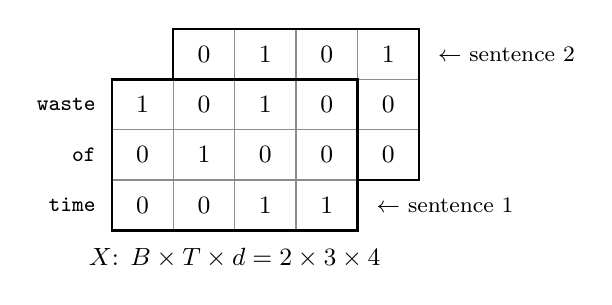
\begin{tikzpicture}
\fill[white] (0.780,0.640) rectangle (3.900,-1.279);
\draw[black!45, fill=white] (0.780,0.640) rectangle (1.560,0.000);
\node[font=\small, text=black] at (1.170,0.320) {$0$};
\draw[black!45, fill=white] (1.560,0.640) rectangle (2.340,0.000);
\node[font=\small, text=black] at (1.950,0.320) {$1$};
\draw[black!45, fill=white] (2.340,0.640) rectangle (3.120,0.000);
\node[font=\small, text=black] at (2.730,0.320) {$0$};
\draw[black!45, fill=white] (3.120,0.640) rectangle (3.900,0.000);
\node[font=\small, text=black] at (3.510,0.320) {$1$};
\draw[black!45, fill=white] (0.780,0.000) rectangle (1.560,-0.640);
\node[font=\small, text=black] at (1.170,-0.320) {$1$};
\draw[black!45, fill=white] (1.560,0.000) rectangle (2.340,-0.640);
\node[font=\small, text=black] at (1.950,-0.320) {$0$};
\draw[black!45, fill=white] (2.340,0.000) rectangle (3.120,-0.640);
\node[font=\small, text=black] at (2.730,-0.320) {$0$};
\draw[black!45, fill=white] (3.120,0.000) rectangle (3.900,-0.640);
\node[font=\small, text=black] at (3.510,-0.320) {$0$};
\draw[black!45, fill=white] (0.780,-0.640) rectangle (1.560,-1.279);
\node[font=\small, text=black] at (1.170,-0.959) {$0$};
\draw[black!45, fill=white] (1.560,-0.640) rectangle (2.340,-1.279);
\node[font=\small, text=black] at (1.950,-0.959) {$0$};
\draw[black!45, fill=white] (2.340,-0.640) rectangle (3.120,-1.279);
\node[font=\small, text=black] at (2.730,-0.959) {$1$};
\draw[black!45, fill=white] (3.120,-0.640) rectangle (3.900,-1.279);
\node[font=\small, text=black] at (3.510,-0.959) {$0$};
\draw[line width=0.9pt] (0.780,0.640) rectangle (3.900,-1.279);
\node[anchor=west, font=\footnotesize] at (4.020,0.320) {$\leftarrow$ sentence 2};
\fill[white] (0.000,0.000) rectangle (3.120,-1.919);
\draw[black!45, fill=white] (0.000,0.000) rectangle (0.780,-0.640);
\node[font=\small, text=black] at (0.390,-0.320) {$1$};
\draw[black!45, fill=white] (0.780,0.000) rectangle (1.560,-0.640);
\node[font=\small, text=black] at (1.170,-0.320) {$0$};
\draw[black!45, fill=white] (1.560,0.000) rectangle (2.340,-0.640);
\node[font=\small, text=black] at (1.950,-0.320) {$1$};
\draw[black!45, fill=white] (2.340,0.000) rectangle (3.120,-0.640);
\node[font=\small, text=black] at (2.730,-0.320) {$0$};
\draw[black!45, fill=white] (0.000,-0.640) rectangle (0.780,-1.279);
\node[font=\small, text=black] at (0.390,-0.959) {$0$};
\draw[black!45, fill=white] (0.780,-0.640) rectangle (1.560,-1.279);
\node[font=\small, text=black] at (1.170,-0.959) {$1$};
\draw[black!45, fill=white] (1.560,-0.640) rectangle (2.340,-1.279);
\node[font=\small, text=black] at (1.950,-0.959) {$0$};
\draw[black!45, fill=white] (2.340,-0.640) rectangle (3.120,-1.279);
\node[font=\small, text=black] at (2.730,-0.959) {$0$};
\draw[black!45, fill=white] (0.000,-1.279) rectangle (0.780,-1.919);
\node[font=\small, text=black] at (0.390,-1.599) {$0$};
\draw[black!45, fill=white] (0.780,-1.279) rectangle (1.560,-1.919);
\node[font=\small, text=black] at (1.170,-1.599) {$0$};
\draw[black!45, fill=white] (1.560,-1.279) rectangle (2.340,-1.919);
\node[font=\small, text=black] at (1.950,-1.599) {$1$};
\draw[black!45, fill=white] (2.340,-1.279) rectangle (3.120,-1.919);
\node[font=\small, text=black] at (2.730,-1.599) {$1$};
\draw[line width=0.9pt] (0.000,0.000) rectangle (3.120,-1.919);
\node[anchor=east, font=\footnotesize\ttfamily] at (-0.080,-0.320) {waste};
\node[anchor=east, font=\footnotesize\ttfamily] at (-0.080,-0.959) {of};
\node[anchor=east, font=\footnotesize\ttfamily] at (-0.080,-1.599) {time};
\node[anchor=west, font=\footnotesize] at (3.240,-1.599) {$\leftarrow$ sentence 1};
\node[anchor=north, font=\small] at (1.560,-2.019) {$X$: $B\times T\times d = 2\times3\times4$};
\end{tikzpicture}
\end{center}

\begin{wrongidea}{2.4}
``Token 1 and token 2 are close, so their meanings are close.'' The number only says which row to open.
In our table, row 1 (\tok{of}) and row 2 (\tok{time}) are at right angles: their dot product is 0. Meaning
lives in the arrows, never in the locker numbers.
\end{wrongidea}

\begin{wrongidea}{2.5}
``The vector of a word changes with the sentence.'' It is tempting because a word's meaning does
change with the sentence. But the row for \tok{time} is the same in \emph{time flies} and in
\emph{waste of time}. What changes with context is the arrow \emph{after} attention has mixed in the other
tokens (Chapter 3). The table gives every token the same starting point; the layers do the rest.
\end{wrongidea}

\begin{checkq}
What does multiplying the one-hot row for \tok{useful} (a 1 in position 5) by $E$ give?
\begin{options}
\item $(0,0,1,0)$, row 5 of the table.
\item $5\times(1,1,1,1)$, because the 1 sits in position 5.
\item The sum of all twelve rows, since every row is multiplied.
\item A number between 0 and 1 saying how useful the word is.
\end{options}
\end{checkq}

\Summary{a token number opens one row of the embedding table, and that row, an arrow of $d$ numbers, is
where the model's knowledge about the token starts.}

%---------------------------------------------------------------------
\subsection*{2.5\quad Where do good arrows come from?}

Our toy arrows were chosen by hand. Requirement 1 of Chapter 1 asks for more: \emph{similar words must
get similar arrows}, so that what is learned about one transfers to the other. How could a machine know
that \tok{money} and \tok{amount} are alike, if nobody tells it?

\Picture You learn what kind of person someone is by talking with them and seeing who they spend time
with. A word is the same. The linguist J. R. Firth put it in 1957: ``You shall know a word by the company
it keeps.'' Words that keep the same company are used for the same things.

\paragraph{The numbers.} Let us build arrows from company alone. We took the \nTwoWvVocab\ most frequent
words of parts 1--8 and counted, for each pair of words, how often they appear within \nTwoWvWin\ words
of each other. Then we kept only the pairs that occur together more often than chance would predict, and
compressed each word's row of counts to $\nTwoWvDim$ numbers (the method is in \texttt{code/ch2\_bpe.py};
Levy and Goldberg, 2014, showed it is closely related to the popular \emph{word2vec} of Mikolov and
colleagues, 2013). Nobody told the program anything about meaning. Here are the nearest arrows it found,
with their cosine (the agreement $\cos\theta$ from Chapter 3):

\begin{center}
\small
\begin{tabular}{@{}l l@{}}
\toprule
word & nearest words in parts 1--8 (cosine)\\
\midrule
\tok{money} & \nTwoNNMoney\\
\tok{model} & \nTwoNNModel\\
\tok{question} & \nTwoNNQuestion\\
\tok{time} & \nTwoNNTime\\
\bottomrule
\end{tabular}
\end{center}

\tok{money} lands next to \tok{amount} and \tok{costs}; \tok{model} next to \tok{models}, \tok{tuned} and
\tok{quen} (how the corpus spells Qwen). Now look at \tok{time}. Its neighbours are \tok{same},
\tok{at}, \tok{point}: in these talks, ``time'' mostly lives in \emph{at the same time} and \emph{at this
point in time}. The arrows learn how a word is \emph{used in this text}, not what a dictionary says. The
cosine between \tok{time} and \tok{money} is \nTwoCosTimeMoney, while any two different one-hot rows
have cosine \nTwoOneHotCos: the counting notebook of Chapter 1 had no way to see any resemblance at all.

\Exactly An embedding is a map from tokens to $\mathbb{R}^d$ chosen so that the geometry carries
information: tokens used in similar contexts get a small angle between them. In this section the map came
from counting. In a transformer the table $E$ is learned by the next-token game itself (Chapter 8): if
two tokens tend to be followed by the same words, the nudges that improve one also improve the other, and
their rows drift together.

\begin{breaks}
The ``company'' picture says nothing about \emph{which} company. \tok{good} and \tok{bad} keep almost the
same company (``a \underline{\ \ } answer'', ``very \underline{\ \ }''), so counting puts them close
together even though they are opposites. A model that needs to tell them apart has to learn it from the
next-word game, where they \emph{are} followed by different words.
\end{breaks}

\begin{wrongidea}{2.6}
``Each of the 64 numbers means something you can name, like sentiment.'' It is tempting because in a churn model,
each clue had a name: number of logins, days since last purchase. Embedding coordinates do not. The
compression is free to spread one idea over many coordinates and to pack many ideas into one. Directions
can carry meaning; single coordinates rarely do.
\end{wrongidea}

\begin{checkq}
Our arrows put \tok{time} near \tok{same} and \tok{point}. What does that tell you?
\begin{options}
\item The method failed, because \tok{time} should be next to \tok{day}.
\item In these talks, \tok{time} is mostly used in phrases like \emph{at the same time}, and the
arrows record usage.
\item Someone labelled \tok{time} and \tok{same} as synonyms.
\item The fourth coordinate of each arrow stores the word's meaning, and they share it.
\end{options}
\end{checkq}

\Summary{arrows built only from which words appear together already place similar words close together,
and a transformer learns its own arrows the same way, from the next-word game.}

%---------------------------------------------------------------------
\subsection*{2.6\quad Requirement 1 is met. What is still missing?}

We now have what Chapter 1 asked for: a way to read any text (byte-pair encoding) and a starting arrow for
every piece, with similar pieces near each other. But look again at \S2.4: the row for \tok{time} is the
same in every sentence. A support reply to \emph{waste of time} and a calendar reminder about \emph{on time}
start from the same arrow. The arrow has to change once the token has seen its neighbours. That is
exactly the job of attention, and it is where Chapter 3 begins.

\begin{principle}{give frequent things a short name and rare things a way to be spelled}
Byte-pair encoding is a compression rule: short codes for what is common, a guaranteed fallback for
everything else. The same rule appears in good systems everywhere: a cache keeps hot items close and goes
to disk for the rest; an agent's tool list gives common actions a named tool and leaves a general
fallback (``run this command'') for the rest. And the embedding idea, \emph{put similar things close
together and search by angle}, is the whole basis of retrieval in an agent's memory system: a memory is
stored as an arrow, and recall means finding the stored arrows with the smallest angle to the question.
\end{principle}

\begin{lookingback}
(a) Chapter 1 measured that \cUnseenThree\% of three-word sequences in part 9 were never seen before.
Does byte-pair encoding fix that problem? (b) Which of the four requirements from Chapter 1 does this
chapter meet? (c) In Chapter 3, which matrix was the first to act on the arrows that come out of the
embedding table?
\end{lookingback}

%---------------------------------------------------------------------
\subsection*{Exercises}

\begin{exercise}
Run one step of byte-pair encoding by hand on the text \tok{waste waste wasted time} (each word followed
by \tok{\_}). Which pair, or pairs, are most frequent, and how many times does each appear? What must a real
tokenizer do when there is a tie?
\end{exercise}

\begin{exercise}
Compute the cosine between the toy arrows of \tok{waste} and \tok{time}. Then compute it between the
one-hot rows of the same two tokens. Which one could ever tell you the words are related?
\end{exercise}

\begin{exercise}
A model has $V=50{,}000$ tokens and $d=768$. How many numbers are in its embedding table? If you double
the vocabulary, what happens to the table, and what (from \S2.2) do you expect to happen to the length of a
typical sentence?
\end{exercise}

\begin{exercise}
Explain to a friend who has never programmed why a model with a byte-level vocabulary can read a word it has
never seen, but may still not understand it. Use the locker picture and say where it stops working.
\end{exercise}

%---------------------------------------------------------------------
\subsection*{Answers to Chapter 2}

\noindent\textbf{Check yourself 2.1.} (a). Each new product name has no row. (b) is wrong: letters never run
out; long names cost length, not failure. (c) reflects M2.1: the model does not read like a person, it only
gets token numbers. (d) confuses length with novelty.

\noindent\textbf{Check yourself 2.2.} (b). Merges follow frequency in the training text. (a) reflects a
belief that the tokenizer judges meaning; it only counts. (c): byte-pair pieces need not be syllables
(\tok{as}, \tok{te\_}). (d): length matters only through frequency; a long common word can be one token.

\noindent\textbf{Check yourself 2.3.} (a). The one-hot row selects row 5. (b) treats the token number as a
quantity (M2.4). (c) forgets that eleven of the twelve multipliers are zero. (d) treats the arrow's numbers
as nameable scores (M2.6).

\noindent\textbf{Check yourself 2.4.} (b). The arrows record how a word is used here. (a) expects
dictionary meaning; (c) is M2.7, since nobody labelled anything; (d) is M2.6.

\noindent\textbf{Looking back.} (a) No. Byte-pair encoding makes every \emph{word} readable, but a counting
model still needs to have seen the same \emph{sequence}; that problem is solved by arrows plus attention.
(b) Requirement 1, similarity. (c) $W_Q$, $W_K$ and $W_V$ act on the arrows.

\noindent\textbf{Exercise 2.1.} \nTwoExTies\ pairs tie, each seen \nTwoExTopCount\ times: \nTwoExTiePairs.
A tokenizer needs a fixed tie-breaking rule (for example, alphabetical order) so that the same text always
gives the same tokens.

\noindent\textbf{Exercise 2.2.} The toy arrows $(1,0,1,0)$ and $(0,0,1,1)$ have dot product 1 and lengths
$\sqrt2$ each, so the cosine is $1/2 = \nTwoCosToyWasteTime$. The one-hot rows have cosine \nTwoOneHotCos,
as any two different one-hot rows do. Only the arrows can express a relation.

\noindent\textbf{Exercise 2.3.} $50{,}000\times768 = \nTwoExThreeTable$ numbers. Doubling the vocabulary doubles
the table. Sentences get shorter, since more letter-groups have their own token, but by less each time:
the curve in \S2.3 flattens.

\noindent\textbf{Exercise 2.4.} Any word can be written as bytes, so it always gets a list of lockers to
open. But each locker holds the arrow of a \emph{piece}, and the meaning of the whole word has to be
assembled by later layers from the pieces and the context. The locker picture stops working there:
lockers are independent, while a word's meaning depends on its neighbours.

\paragraph{What you now know.}
\begin{itemize}
\item Why neither whole words nor single letters work, with the numbers that show it.
\item How byte-pair encoding builds a vocabulary by merging the most frequent pair, again and again.
\item That an embedding is one row of a table, fetched by a one-hot row times a matrix.
\item That token numbers carry no meaning, and that arrows built from word company place similar words
close together.
\end{itemize}

\clearpage\newpage
\section*{3\quad Attention: letting tokens talk}
\addcontentsline{toc}{section}{3 Attention}
\startchapter{3}

\begin{chaptermap}
\emph{The problem:} the token \tok{time} must learn, from the tokens before it, that it is time \emph{wasted}.
\emph{The steps:} the plain average and why it fails (\S3.1); three tools from geometry: the dot product, the
matrix, the transpose (\S3.2--3.4); queries, keys and values (\S3.5); a full worked example (\S3.6); why softmax
and why $\sqrt{d_k}$ (\S3.7--3.8); a whole batch at once (\S3.9); learning as turning arrows (\S3.10).
\emph{Where it ends:} with a working attention layer, meeting Requirements 3 and 4 of Chapter 1, and a new
failure: it has forgotten word order.
\end{chaptermap}

\machine{3}{You are here: Chapter 3 adds \emph{attention}, the block where tokens talk to each other. The embedding of Chapter 2 feeds it; everything below it is still ahead.}

\begin{beforeyoustart}
\begin{enumerate}[label=\arabic*.,leftmargin=1.6em]
\item On squared paper, draw the arrow $(3,1)$: start at a corner, go 3 squares right and 1 square up.\\
\emph{Refresher:} the first number is ``across'', the second ``up''. Negative numbers go left or down.
\item What is $2\times(-1)+3\times4$?\\
\emph{Refresher:} multiply first, then add. A positive times a negative is negative: $-2+12=\nThreePk$.
\item What are $\sqrt{16}$ and $\sqrt{256}$?\\
\emph{Refresher:} the square root asks ``which number times itself gives this?'' $4\times4=16$ and
$16\times16=256$.
\item What is $e$, and what are $e^0$ and $e^2$?\\
\emph{Refresher:} $e\approx\nThreeE$ is a fixed number, like $\pi$. Any number to the power 0 is 1, and
$e^2=e\times e\approx\nThreeEtwo$. Powers of $e$ are always positive.
\item What is the average of 2, 4 and 9?\\
\emph{Refresher:} add them and divide by how many there are: $15/3=\nThreeAvg$.
\end{enumerate}
\end{beforeyoustart}

Chapter 1 left us with four requirements. Chapter 2 met the first one: every token becomes an arrow of $d$
numbers, a row of the embedding table, and similar tokens get similar arrows. This chapter meets Requirements 3
and 4: every token must reach every earlier token \emph{directly}, and all of that must happen \emph{at once}.
We use the three tokens of our problem. Their rows of the toy embedding table, stacked one row per token,
form the matrix $X$:
\begin{center}% AUTO-GENERATED by code/figlib.py helpers -- do not edit
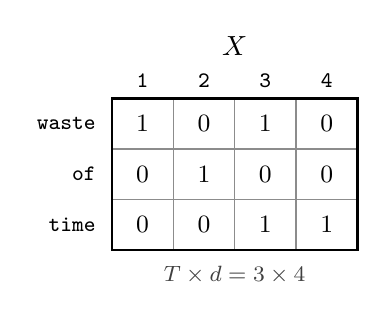
\begin{tikzpicture}
\draw[black!45, fill=white] (0.000,0.000) rectangle (0.780,-0.640);
\node[font=\small, text=black] at (0.390,-0.320) {$1$};
\draw[black!45, fill=white] (0.780,0.000) rectangle (1.560,-0.640);
\node[font=\small, text=black] at (1.170,-0.320) {$0$};
\draw[black!45, fill=white] (1.560,0.000) rectangle (2.340,-0.640);
\node[font=\small, text=black] at (1.950,-0.320) {$1$};
\draw[black!45, fill=white] (2.340,0.000) rectangle (3.120,-0.640);
\node[font=\small, text=black] at (2.730,-0.320) {$0$};
\draw[black!45, fill=white] (0.000,-0.640) rectangle (0.780,-1.279);
\node[font=\small, text=black] at (0.390,-0.959) {$0$};
\draw[black!45, fill=white] (0.780,-0.640) rectangle (1.560,-1.279);
\node[font=\small, text=black] at (1.170,-0.959) {$1$};
\draw[black!45, fill=white] (1.560,-0.640) rectangle (2.340,-1.279);
\node[font=\small, text=black] at (1.950,-0.959) {$0$};
\draw[black!45, fill=white] (2.340,-0.640) rectangle (3.120,-1.279);
\node[font=\small, text=black] at (2.730,-0.959) {$0$};
\draw[black!45, fill=white] (0.000,-1.279) rectangle (0.780,-1.919);
\node[font=\small, text=black] at (0.390,-1.599) {$0$};
\draw[black!45, fill=white] (0.780,-1.279) rectangle (1.560,-1.919);
\node[font=\small, text=black] at (1.170,-1.599) {$0$};
\draw[black!45, fill=white] (1.560,-1.279) rectangle (2.340,-1.919);
\node[font=\small, text=black] at (1.950,-1.599) {$1$};
\draw[black!45, fill=white] (2.340,-1.279) rectangle (3.120,-1.919);
\node[font=\small, text=black] at (2.730,-1.599) {$1$};
\draw[line width=0.9pt] (0.000,0.000) rectangle (3.120,-1.919);
\node[anchor=east, font=\footnotesize\ttfamily] at (-0.080,-0.320) {waste};
\node[anchor=east, font=\footnotesize\ttfamily] at (-0.080,-0.959) {of};
\node[anchor=east, font=\footnotesize\ttfamily] at (-0.080,-1.599) {time};
\node[anchor=south, font=\footnotesize\ttfamily] at (0.390,0.020) {1};
\node[anchor=south, font=\footnotesize\ttfamily] at (1.170,0.020) {2};
\node[anchor=south, font=\footnotesize\ttfamily] at (1.950,0.020) {3};
\node[anchor=south, font=\footnotesize\ttfamily] at (2.730,0.020) {4};
\node[anchor=south, font=\normalsize] at (1.560,0.420) {$X$};
\node[anchor=north, font=\footnotesize, text=black!75] at (1.560,-1.999) {$T\times d=3\times4$};
\end{tikzpicture}
\end{center}
These numbers are chosen by hand so you can follow every multiplication with a pencil. Real ones are learned
and much longer: Qwen3-0.6B uses 1024 numbers per token (Chapter 10).

%---------------------------------------------------------------------
\subsection*{3.1\quad The simple thing, and how it breaks}

Look at the token \tok{time}. On its own, its arrow is the same in every sentence: \emph{time flies}, \emph{on
time}, \emph{waste of time}. But the reply we want depends on \emph{wasted} time, time in a complaint. You learn
what kind of person someone is by talking to them, not by reading their name; a token learns what it means here
by listening to the tokens around it. So \tok{time} must pull in information from the tokens before it. What is
the simplest possible way? Take the average.

\Picture A class decides what to name the class pet, and every vote counts the same, whether the voter loves
the pet or has never seen it.

\Exactly
\[
\bm{u}_{\text{time}} = \tfrac{1}{3}\left(\bm{x}_{\text{waste}} + \bm{x}_{\text{of}} + \bm{x}_{\text{time}}\right) = \uTime \shape{1\times d}
\]
This says \tok{of} matters to \tok{time} exactly as much as \tok{waste} does. That is wrong, and no amount of
training can fix it, because there is nothing to train: the weights $\tfrac13,\tfrac13,\tfrac13$ are fixed by
the length of the sentence.

\begin{breaks}
In a class vote, every voter at least chose to vote. Here \tok{of} gets a full third of the say without having
anything to say about \tok{time}.
\end{breaks}

\Why \emph{We need the weights themselves to depend on the content}: \tok{time} should be able to \emph{ask}
which earlier tokens matter to it, and get a different answer in every sentence. To build ``asking'' and
``matching'' out of numbers, we need three tools from geometry. They are short, and they are the whole of the
mathematics in this chapter.

\begin{wrongidea}{3.1}
\emph{A token can use its own vector to predict the next word; mixing in other tokens is optional.} The vector
already encodes the word's meaning, so why mix? Because \tok{time}'s own vector is identical after \emph{on} and
after \emph{waste of}, and the right next word is different. Only the neighbours can tell them apart.
\end{wrongidea}

\begin{checkq}
Why can the token \tok{time} not predict \tok{Sorry} from its own arrow alone?
\begin{options}
\item It can: its arrow already encodes what \tok{time} means.
\item Its arrow is the same after \emph{on} and after \emph{waste of}, but the right next word differs.
\item It needs the plain average of all tokens, which settles the question.
\item Because its arrow does not know its position in the sentence.
\end{options}
\end{checkq}

\Summary{A token's own arrow is the same in every sentence, and a plain average cannot decide who matters, so
the mixing weights must depend on content.}

%---------------------------------------------------------------------
\subsection*{3.2\quad Tool 1: how much two arrows agree}

Start from something you may have built already: a churn score. For each customer you have some clues (days
since last login, support tickets this month, purchases this month) and for each clue an importance. The score
asks, for every clue, how important it is, and then combines everything together.

\Predict A customer has clues $\nThreeClues$ and the importances are $\nThreeW$. What is the score? Is it
positive or negative?

Multiply each clue by its importance and add: $\nThreeTerms = \nThreeScore$. Drawn as a row of clues
meeting a column of importances:
\begin{center}\resizebox{\linewidth}{!}{% AUTO-GENERATED by code/figlib.py helpers -- do not edit
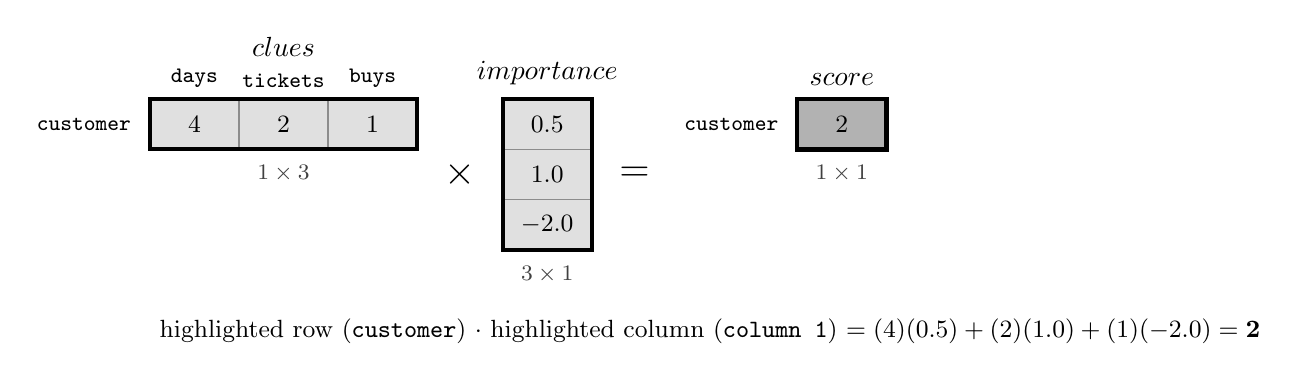
\begin{tikzpicture}[x=1.45cm]
\draw[black!45, fill=black!12] (0.000,0.000) rectangle (0.780,-0.640);
\node[font=\small, text=black] at (0.390,-0.320) {$4$};
\draw[black!45, fill=black!12] (0.780,0.000) rectangle (1.560,-0.640);
\node[font=\small, text=black] at (1.170,-0.320) {$2$};
\draw[black!45, fill=black!12] (1.560,0.000) rectangle (2.340,-0.640);
\node[font=\small, text=black] at (1.950,-0.320) {$1$};
\draw[line width=1.4pt] (0.000,0.000) rectangle (2.340,-0.640);
\draw[line width=0.9pt] (0.000,0.000) rectangle (2.340,-0.640);
\node[anchor=east, font=\footnotesize\ttfamily] at (-0.080,-0.320) {customer};
\node[anchor=south, font=\footnotesize\ttfamily] at (0.390,0.020) {days};
\node[anchor=south, font=\footnotesize\ttfamily] at (1.170,0.020) {tickets};
\node[anchor=south, font=\footnotesize\ttfamily] at (1.950,0.020) {buys};
\node[anchor=south, font=\normalsize] at (1.170,0.420) {$\text{clues}$};
\node[anchor=north, font=\footnotesize, text=black!75] at (1.170,-0.720) {$1\times3$};
\draw[black!45, fill=black!12] (3.090,0.000) rectangle (3.870,-0.640);
\node[font=\small, text=black] at (3.480,-0.320) {$0.5$};
\draw[black!45, fill=black!12] (3.090,-0.640) rectangle (3.870,-1.279);
\node[font=\small, text=black] at (3.480,-0.959) {$1.0$};
\draw[black!45, fill=black!12] (3.090,-1.279) rectangle (3.870,-1.919);
\node[font=\small, text=black] at (3.480,-1.599) {$-2.0$};
\draw[line width=1.4pt] (3.090,0.000) rectangle (3.870,-1.919);
\draw[line width=0.9pt] (3.090,0.000) rectangle (3.870,-1.919);
\node[anchor=south, font=\normalsize] at (3.480,0.050) {$\text{importance}$};
\node[anchor=north, font=\footnotesize, text=black!75] at (3.480,-1.999) {$3\times1$};
\draw[black!45, fill=black!30] (5.670,0.000) rectangle (6.450,-0.640);
\node[font=\small, text=black] at (6.060,-0.320) {$2$};
\draw[line width=1.6pt] (5.670,0.000) rectangle (6.450,-0.640);
\draw[line width=0.9pt] (5.670,0.000) rectangle (6.450,-0.640);
\node[anchor=east, font=\footnotesize\ttfamily] at (5.590,-0.320) {customer};
\node[anchor=south, font=\normalsize] at (6.060,0.050) {$\text{score}$};
\node[anchor=north, font=\footnotesize, text=black!75] at (6.060,-0.720) {$1\times1$};
\node[font=\Large] at (2.715,-0.959) {$\times$};
\node[font=\Large] at (4.245,-0.959) {$=$};
\node[anchor=north west, font=\small, align=left] at (0,-2.669) {highlighted row (\texttt{customer}) $\cdot$ highlighted column (\texttt{column 1}) $= (4)(0.5) + (2)(1.0) + (1)(-2.0) = \mathbf{2}$};
\end{tikzpicture}
}\end{center}

That operation, multiply matching entries and add, is the \emph{dot product}. Now let us see it as geometry.

\Picture An arrow is a set of directions: ``3 steps east, 1 step north'' is the arrow $(3,1)$. Two friends walk
out of school, one along $\bm{a}=(3,1)$ and one along $\bm{b}=(1,2)$. How much are they going \emph{the same
way}? Shine a torch from straight above $\bm{a}$'s path and look at the shadow that $\bm{b}$ casts on it. A long
shadow means they mostly agree. No shadow means they are walking at right angles. A shadow pointing backwards
means they are walking apart.

\begin{figure}[h]
\centering
\begin{tikzpicture}[scale=1.05, font=\footnotesize]
\draw[black!50] (-0.3,0) -- (3.6,0); \draw[black!50] (0,-0.3) -- (0,1.8);
\draw[-{Stealth}, thick] (0,0) -- (3,1) node[right] {$\bm{a}=(3,1)$, length \geoNa};
\draw[-{Stealth}, thick, black!70] (0,0) -- (1,2) node[above, text=black] {$\bm{b}=(1,2)$, length \geoNb};
\draw[dashed] (1,2) -- (1.5,0.5);
\draw[line width=2.4pt, black!35] (0,0) -- (1.5,0.5);
\node[below right, align=left] at (1.35,0.35) {shadow of $\bm{b}$ on $\bm{a}$:\\length \geoShadow};
\draw (0.55,0.183) arc[start angle=18.43, end angle=63.43, radius=0.58];
\node at (0.62,0.62) {\geoAng$^\circ$};
\begin{scope}[xshift=7.2cm, scale=0.55]
\foreach \y/\lab/\bx/\by in {3.2/{same way: big, positive}/2/0.6, 0/{right angle: zero}/0/1.6, -3.2/{opposite: negative}/-1.5/0.9} {
  \draw[-{Stealth}, thick] (0,\y) -- (2,\y+0.6);
  \draw[-{Stealth}, thick, black!60] (0,\y) -- (\bx,\y+\by);
  \node[right, font=\footnotesize] at (2.6,\y+0.3) {\lab};
}
\end{scope}
\end{tikzpicture}
\caption{The dot product as a shadow. Left: our two arrows, at \geoAng$^\circ$. Right: the three cases.}
\label{fig:dot}
\end{figure}

\Predict Before computing $(3,1)\cdot(1,2)$: from the picture, will it be positive, zero or negative?

\Exactly The dot product multiplies matching entries and adds:
\[
\bm{a}\cdot\bm{b} = a_1b_1 + a_2b_2 + \cdots + a_db_d .
\]
As a picture, the row $\bm{a}$ meets the column $\bm{b}$ (we write $\bm{b}$ standing up, as $\bm{b}^\top$):
\begin{center}% AUTO-GENERATED by code/figlib.py helpers -- do not edit
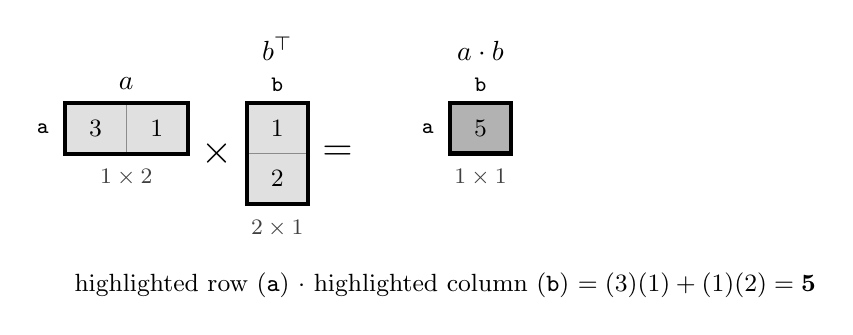
\begin{tikzpicture}
\draw[black!45, fill=black!12] (0.000,0.000) rectangle (0.780,-0.640);
\node[font=\small, text=black] at (0.390,-0.320) {$3$};
\draw[black!45, fill=black!12] (0.780,0.000) rectangle (1.560,-0.640);
\node[font=\small, text=black] at (1.170,-0.320) {$1$};
\draw[line width=1.4pt] (0.000,0.000) rectangle (1.560,-0.640);
\draw[line width=0.9pt] (0.000,0.000) rectangle (1.560,-0.640);
\node[anchor=east, font=\footnotesize\ttfamily] at (-0.080,-0.320) {a};
\node[anchor=south, font=\normalsize] at (0.780,0.050) {$\bm{a}$};
\node[anchor=north, font=\footnotesize, text=black!75] at (0.780,-0.720) {$1\times2$};
\draw[black!45, fill=black!12] (2.310,0.000) rectangle (3.090,-0.640);
\node[font=\small, text=black] at (2.700,-0.320) {$1$};
\draw[black!45, fill=black!12] (2.310,-0.640) rectangle (3.090,-1.279);
\node[font=\small, text=black] at (2.700,-0.959) {$2$};
\draw[line width=1.4pt] (2.310,0.000) rectangle (3.090,-1.279);
\draw[line width=0.9pt] (2.310,0.000) rectangle (3.090,-1.279);
\node[anchor=south, font=\footnotesize\ttfamily] at (2.700,0.020) {b};
\node[anchor=south, font=\normalsize] at (2.700,0.420) {$\bm{b}^{\top}$};
\node[anchor=north, font=\footnotesize, text=black!75] at (2.700,-1.359) {$2\times1$};
\draw[black!45, fill=black!30] (4.890,0.000) rectangle (5.670,-0.640);
\node[font=\small, text=black] at (5.280,-0.320) {$5$};
\draw[line width=1.6pt] (4.890,0.000) rectangle (5.670,-0.640);
\draw[line width=0.9pt] (4.890,0.000) rectangle (5.670,-0.640);
\node[anchor=east, font=\footnotesize\ttfamily] at (4.810,-0.320) {a};
\node[anchor=south, font=\footnotesize\ttfamily] at (5.280,0.020) {b};
\node[anchor=south, font=\normalsize] at (5.280,0.420) {$\bm{a}\cdot\bm{b}$};
\node[anchor=north, font=\footnotesize, text=black!75] at (5.280,-0.720) {$1\times1$};
\node[font=\Large] at (1.935,-0.640) {$\times$};
\node[font=\Large] at (3.465,-0.640) {$=$};
\node[anchor=north west, font=\small, align=left] at (0,-2.029) {highlighted row (\texttt{a}) $\cdot$ highlighted column (\texttt{b}) $= (3)(1) + (1)(2) = \mathbf{5}$};
\end{tikzpicture}
\end{center}
The surprising fact is that this sum measures agreement:
\[
\bm{a}\cdot\bm{b} \;=\; \lVert\bm{a}\rVert\,\lVert\bm{b}\rVert\cos\theta ,
\]
where $\theta$ is the angle between the arrows. Check it: $\geoNa \times \geoNb \times \cos \geoAng^\circ =
\geoDot$. Why should multiply-and-add know about angles? Draw the third side of the triangle, $\bm{a}-\bm{b}$.
Expanding its squared length entry by entry gives $\lVert\bm{a}-\bm{b}\rVert^2 = \lVert\bm{a}\rVert^2 +
\lVert\bm{b}\rVert^2 - 2\,\bm{a}\cdot\bm{b}$, while the law of cosines says the same squared length is
$\lVert\bm{a}\rVert^2 + \lVert\bm{b}\rVert^2 - 2\lVert\bm{a}\rVert\lVert\bm{b}\rVert\cos\theta$. Compare the two,
and the formula falls out. Nothing in the argument cares whether there are 2 entries or 1024, so the picture
holds in any number of dimensions.

\Sanity The churn customer is an arrow too: three clues, three directions. Its score of \nThreeScore\ is the
shadow of the customer arrow on the importance arrow, times the importance arrow's length.

\begin{breaks}
You can draw shadows in two or three dimensions. In 1024 dimensions you cannot, but the arithmetic still works
and still means ``how much do these agree''. Trust the formula where the drawing stops.
\end{breaks}

\Why The dot product has exactly two knobs: \emph{direction} ($\cos\theta$, how much the arrows agree) and
\emph{length} ($\lVert\bm{a}\rVert\lVert\bm{b}\rVert$, how strongly they say it). Keep these two knobs in mind; at
the end of the chapter, learning will turn out to be nothing but turning them.

\begin{wrongidea}{3.8}
\emph{A bigger dot product always means more similar.} Dot products are often introduced as similarity scores,
so bigger feels like closer. But a long arrow pointing a little off can beat a short arrow pointing exactly the
same way. Similarity of direction is $\cos\theta$; the dot product also multiplies in both lengths.
\end{wrongidea}

\begin{checkq}
Take $\bm{a}=(1,0)$, $\bm{b}=(3,3)$ and $\bm{c}=(1,0)$. Which arrow points most nearly the same way as $\bm{a}$?
\begin{options}
\item $\bm{b}$, because $\bm{a}\cdot\bm{b}=\nThreeQbDot$ is bigger than $\bm{a}\cdot\bm{c}=\nThreeQcDot$.
\item $\bm{c}$: the angle is \nThreeQcAng$^\circ$, against \nThreeQbAng$^\circ$ for $\bm{b}$.
\item They agree equally, since both dot products are positive.
\item You cannot tell without drawing them.
\end{options}
\end{checkq}

\Summary{Multiply-and-add measures how much two arrows agree in direction, scaled by how long they are.}

%---------------------------------------------------------------------
\subsection*{3.3\quad Tool 2: a matrix is a machine that moves arrows}

\Picture A matrix is a set of recipe cards. Each card says ``take this much of your first number, this much of
your second, \ldots, and add''. An arrow goes in; each card produces one number of the new arrow. A matrix with
64 columns is 64 recipes: 64 different ways of looking at the same token.

\Exactly Multiplying a $1\times d$ arrow by a $d\times d_k$ matrix $W$ gives a $1\times d_k$ arrow whose $j$-th
entry is the dot product of the input with column $j$ of $W$ (card $j$).

\Predict Feed \tok{waste}, $(1,0,1,0)$, into the key matrix below. Before multiplying: which rows of $W_K$ will
end up mattering?
\begin{center}% AUTO-GENERATED by code/figlib.py helpers -- do not edit
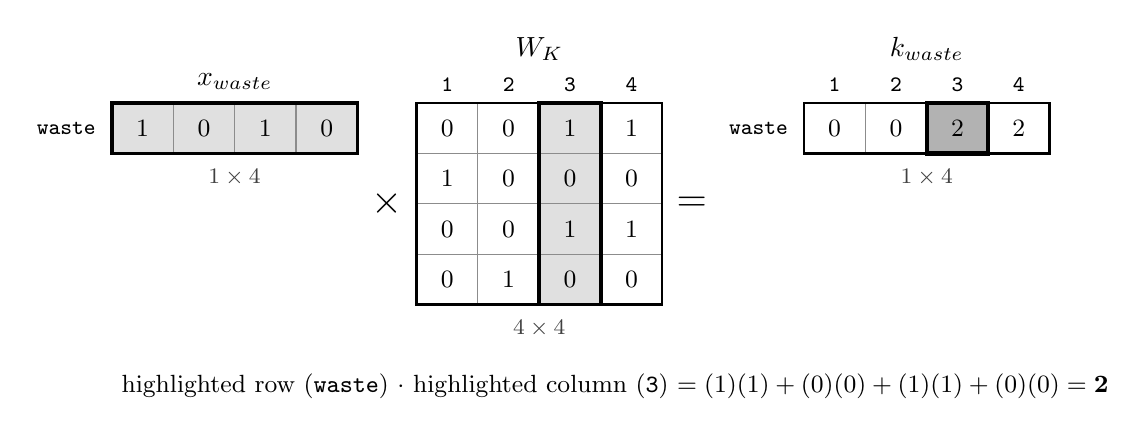
\begin{tikzpicture}
\draw[black!45, fill=black!12] (0.000,0.000) rectangle (0.780,-0.640);
\node[font=\small, text=black] at (0.390,-0.320) {$1$};
\draw[black!45, fill=black!12] (0.780,0.000) rectangle (1.560,-0.640);
\node[font=\small, text=black] at (1.170,-0.320) {$0$};
\draw[black!45, fill=black!12] (1.560,0.000) rectangle (2.340,-0.640);
\node[font=\small, text=black] at (1.950,-0.320) {$1$};
\draw[black!45, fill=black!12] (2.340,0.000) rectangle (3.120,-0.640);
\node[font=\small, text=black] at (2.730,-0.320) {$0$};
\draw[line width=1.4pt] (0.000,0.000) rectangle (3.120,-0.640);
\draw[line width=0.9pt] (0.000,0.000) rectangle (3.120,-0.640);
\node[anchor=east, font=\footnotesize\ttfamily] at (-0.080,-0.320) {waste};
\node[anchor=south, font=\normalsize] at (1.560,0.050) {$\bm{x}_{\text{waste}}$};
\node[anchor=north, font=\footnotesize, text=black!75] at (1.560,-0.720) {$1\times4$};
\draw[black!45, fill=white] (3.870,0.000) rectangle (4.650,-0.640);
\node[font=\small, text=black] at (4.260,-0.320) {$0$};
\draw[black!45, fill=white] (4.650,0.000) rectangle (5.430,-0.640);
\node[font=\small, text=black] at (5.040,-0.320) {$0$};
\draw[black!45, fill=black!12] (5.430,0.000) rectangle (6.210,-0.640);
\node[font=\small, text=black] at (5.820,-0.320) {$1$};
\draw[black!45, fill=white] (6.210,0.000) rectangle (6.990,-0.640);
\node[font=\small, text=black] at (6.600,-0.320) {$1$};
\draw[black!45, fill=white] (3.870,-0.640) rectangle (4.650,-1.279);
\node[font=\small, text=black] at (4.260,-0.959) {$1$};
\draw[black!45, fill=white] (4.650,-0.640) rectangle (5.430,-1.279);
\node[font=\small, text=black] at (5.040,-0.959) {$0$};
\draw[black!45, fill=black!12] (5.430,-0.640) rectangle (6.210,-1.279);
\node[font=\small, text=black] at (5.820,-0.959) {$0$};
\draw[black!45, fill=white] (6.210,-0.640) rectangle (6.990,-1.279);
\node[font=\small, text=black] at (6.600,-0.959) {$0$};
\draw[black!45, fill=white] (3.870,-1.279) rectangle (4.650,-1.919);
\node[font=\small, text=black] at (4.260,-1.599) {$0$};
\draw[black!45, fill=white] (4.650,-1.279) rectangle (5.430,-1.919);
\node[font=\small, text=black] at (5.040,-1.599) {$0$};
\draw[black!45, fill=black!12] (5.430,-1.279) rectangle (6.210,-1.919);
\node[font=\small, text=black] at (5.820,-1.599) {$1$};
\draw[black!45, fill=white] (6.210,-1.279) rectangle (6.990,-1.919);
\node[font=\small, text=black] at (6.600,-1.599) {$1$};
\draw[black!45, fill=white] (3.870,-1.919) rectangle (4.650,-2.558);
\node[font=\small, text=black] at (4.260,-2.239) {$0$};
\draw[black!45, fill=white] (4.650,-1.919) rectangle (5.430,-2.558);
\node[font=\small, text=black] at (5.040,-2.239) {$1$};
\draw[black!45, fill=black!12] (5.430,-1.919) rectangle (6.210,-2.558);
\node[font=\small, text=black] at (5.820,-2.239) {$0$};
\draw[black!45, fill=white] (6.210,-1.919) rectangle (6.990,-2.558);
\node[font=\small, text=black] at (6.600,-2.239) {$0$};
\draw[line width=1.4pt] (5.430,0.000) rectangle (6.210,-2.558);
\draw[line width=0.9pt] (3.870,0.000) rectangle (6.990,-2.558);
\node[anchor=south, font=\footnotesize\ttfamily] at (4.260,0.020) {1};
\node[anchor=south, font=\footnotesize\ttfamily] at (5.040,0.020) {2};
\node[anchor=south, font=\footnotesize\ttfamily] at (5.820,0.020) {3};
\node[anchor=south, font=\footnotesize\ttfamily] at (6.600,0.020) {4};
\node[anchor=south, font=\normalsize] at (5.430,0.420) {$W_K$};
\node[anchor=north, font=\footnotesize, text=black!75] at (5.430,-2.638) {$4\times4$};
\draw[black!45, fill=white] (8.790,0.000) rectangle (9.570,-0.640);
\node[font=\small, text=black] at (9.180,-0.320) {$0$};
\draw[black!45, fill=white] (9.570,0.000) rectangle (10.350,-0.640);
\node[font=\small, text=black] at (9.960,-0.320) {$0$};
\draw[black!45, fill=black!30] (10.350,0.000) rectangle (11.130,-0.640);
\node[font=\small, text=black] at (10.740,-0.320) {$2$};
\draw[black!45, fill=white] (11.130,0.000) rectangle (11.910,-0.640);
\node[font=\small, text=black] at (11.520,-0.320) {$2$};
\draw[line width=1.6pt] (10.350,0.000) rectangle (11.130,-0.640);
\draw[line width=0.9pt] (8.790,0.000) rectangle (11.910,-0.640);
\node[anchor=east, font=\footnotesize\ttfamily] at (8.710,-0.320) {waste};
\node[anchor=south, font=\footnotesize\ttfamily] at (9.180,0.020) {1};
\node[anchor=south, font=\footnotesize\ttfamily] at (9.960,0.020) {2};
\node[anchor=south, font=\footnotesize\ttfamily] at (10.740,0.020) {3};
\node[anchor=south, font=\footnotesize\ttfamily] at (11.520,0.020) {4};
\node[anchor=south, font=\normalsize] at (10.350,0.420) {$\bm{k}_{\text{waste}}$};
\node[anchor=north, font=\footnotesize, text=black!75] at (10.350,-0.720) {$1\times4$};
\node[font=\Large] at (3.495,-1.279) {$\times$};
\node[font=\Large] at (7.365,-1.279) {$=$};
\node[anchor=north west, font=\small, align=left] at (0,-3.308) {highlighted row (\texttt{waste}) $\cdot$ highlighted column (\texttt{3}) $= (1)(1) + (0)(0) + (1)(1) + (0)(0) = \mathbf{2}$};
\end{tikzpicture}
\end{center}
Each output number is the input row meeting one column (one recipe card). The highlighted column 3 gives 2; the
four columns give $\kWasteRow$. There is a second way to see the same multiplication. Because $\bm{x}_{\text{waste}}$ has a 1 in positions 1 and 3,
the result is \emph{row 1 plus row 3} of $W_K$, namely $(0,0,1,1)+(0,0,1,1)$. A matrix sends each input direction
somewhere; it can rotate arrows, stretch them, squash them, or flatten some directions to nothing.

\begin{breaks}
Recipe cards suggest each card is separate. A matrix also has a single geometric effect on the whole space (a
turn, a stretch, a squash) that no single card shows.
\end{breaks}

\Why A matrix lets the \emph{same} token be seen in different ways. The arrow for \tok{waste} is fixed, but $W_K$
produces one view of it and $W_Q$ another. If the model needs a new view, it does not change the word; it learns
a new machine.

\Summary{A matrix turns one arrow into another, one recipe (column) per output number, so one token can be viewed
in many learned ways.}

%---------------------------------------------------------------------
\subsection*{3.4\quad Tool 3: the transpose, and the table of all meetings}

\Picture At the start of a tournament every player shakes hands with every other player. The organiser draws a
table: players down the side, players across the top, and in each cell writes how friendly that handshake was.

\Exactly Stack all the queries as rows of $Q$ ($T\times d_k$) and all the keys as rows of $K$ ($T\times d_k$). We
want the table $S$ with $S_{ij} = \bm{q}_i\cdot\bm{k}_j$. Matrix multiplication always pairs a \emph{row of the
left} with a \emph{column of the right}. Our queries are already rows. Our keys are rows too, so we flip them into
columns: that flip is the \emph{transpose} $K^\top$ ($d_k\times T$). Now
\[
S = Q K^\top \shape{(T\times d_k)(d_k\times T) = T\times T},
\]
and the cell in row $i$, column $j$ is row $i$ of $Q$ meeting column $j$ of $K^\top$, which is
$\bm{q}_i\cdot\bm{k}_j$. There is a deeper way to see it. A column of $K^\top$ is a key, and dot-producting with
an arrow measures the shadow along it. So $K^\top$ is a set of $T$ \emph{rulers}, one per key, and multiplying a
query by $K^\top$ measures that query along every key at once.

\begin{breaks}
A handshake is the same from both sides. Here it is not: the score of \tok{time} looking at \tok{waste} uses
\tok{time}'s query and \tok{waste}'s key, while \tok{waste} looking at \tok{time} uses the other pair. The table is
not symmetric.
\end{breaks}

\Why This is Requirement 4 in one line. An RNN produces its numbers one step after another; here all $T\times T$
scores come out of a single matrix multiplication, which is the operation a GPU's thousands of workers are built
to share.

\begin{wrongidea}{3.9}
\emph{The transpose changes the vectors.} The matrix looks different afterwards, so something must have changed.
But every key arrow is exactly the same arrow before and after; the transpose only stands it up as a column, so
that ``row meets column'' pairs each query with each key.
\end{wrongidea}

\begin{checkq}
In $QK^\top$ for our toy, why $K^\top$ and not $K$?
\begin{options}
\item $Q$ is $3\times4$ and $K$ is $3\times4$, so $QK$ is not defined; $QK^\top$ is $3\times3$, one score per pair of tokens.
\item The transpose turns the keys so they match the queries better.
\item The transpose rescales the keys to length 1.
\item Either works; $QK$ gives the same numbers in a different order.
\end{options}
\end{checkq}

\Summary{Flipping the keys into columns lets one multiplication produce every query-key score at once, without
changing any arrow.}

%---------------------------------------------------------------------
\subsection*{3.5\quad The fix: three questions per token}

Now we can build ``asking''. Attention gives every token three different views of itself, each made by its own
learned machine:
\begin{itemize}
\item \textbf{Query} $\bm{q}=\bm{x}W_Q$: \emph{what am I looking for?}
\item \textbf{Key} $\bm{k}=\bm{x}W_K$: \emph{what can I be found by?}
\item \textbf{Value} $\bm{v}=\bm{x}W_V$: \emph{what do I hand over if I am chosen?}
\end{itemize}

\Picture A library. The query is what you type into the search box. The key is the label on each book's spine.
The value is what is written inside the book. You match your search against the labels, but you take home the
contents.

\begin{breaks}
In a library you take home a few whole books. Attention takes home a blend: a little of every book, in
proportions set by how well each label matched.
\end{breaks}

\Why Why three, and not one arrow for everything? Because what makes you \emph{findable} is not the same as what
you \emph{offer}, and neither is the same as what you \emph{need}. \tok{waste} should be found by any token asking
``is there a judgement nearby?'', but what it hands over is the content of that judgement, and what \tok{waste}
itself is looking for is something else again. One arrow cannot point in three directions.

\begin{wrongidea}{3.4}
\emph{Query, key and value are three copies of the same thing; one vector would do.} All three are made from the
same token arrow, so they look like copies. The paragraph above explains why they are not: each is a different
machine applied to the same arrow, and each points where its own job needs it.
\end{wrongidea}

\begin{wrongidea}{3.6}
\emph{Values are the words' original meanings.} Values are made from the embeddings, so it is tempting to read
them as the dictionary meaning. They are a learned \emph{view} made for handing over, built by $W_V$. In the toy,
$\bm{x}_{\text{waste}}=(1,0,1,0)$ but $\bm{v}_{\text{waste}}$ is different, as you will see below.
\end{wrongidea}

In the toy we use the machines in Figure~\ref{fig:qkv} (chosen for pencil-friendliness; real ones are
learned). Each picture feeds all three tokens through one machine at once: $X$ ($3\times4$) times $W$ ($4\times4$)
gives one new row per token. One row meeting one column is highlighted and written out; check one more cell
yourself before reading on.
\begin{figure}[!htb]\centering
% AUTO-GENERATED by code/figlib.py helpers -- do not edit
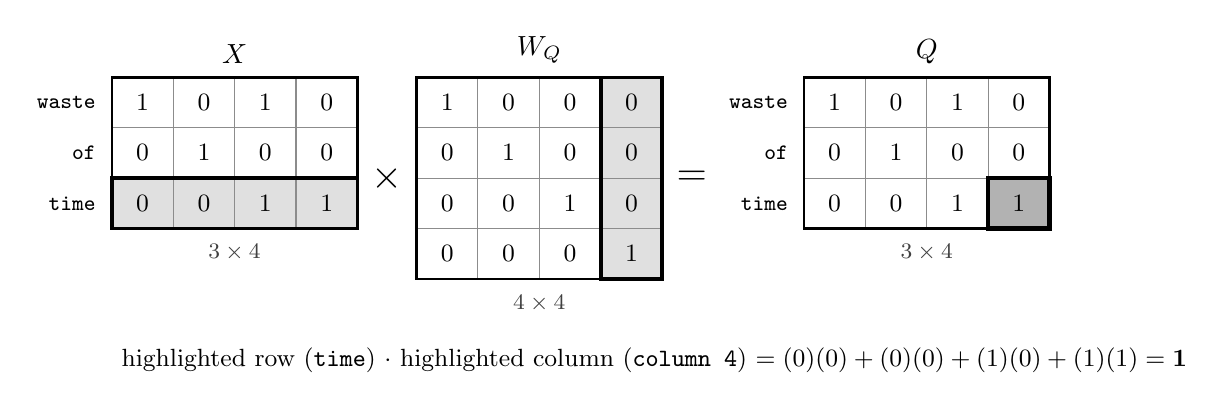
\begin{tikzpicture}
\draw[black!45, fill=white] (0.000,0.000) rectangle (0.780,-0.640);
\node[font=\small, text=black] at (0.390,-0.320) {$1$};
\draw[black!45, fill=white] (0.780,0.000) rectangle (1.560,-0.640);
\node[font=\small, text=black] at (1.170,-0.320) {$0$};
\draw[black!45, fill=white] (1.560,0.000) rectangle (2.340,-0.640);
\node[font=\small, text=black] at (1.950,-0.320) {$1$};
\draw[black!45, fill=white] (2.340,0.000) rectangle (3.120,-0.640);
\node[font=\small, text=black] at (2.730,-0.320) {$0$};
\draw[black!45, fill=white] (0.000,-0.640) rectangle (0.780,-1.279);
\node[font=\small, text=black] at (0.390,-0.959) {$0$};
\draw[black!45, fill=white] (0.780,-0.640) rectangle (1.560,-1.279);
\node[font=\small, text=black] at (1.170,-0.959) {$1$};
\draw[black!45, fill=white] (1.560,-0.640) rectangle (2.340,-1.279);
\node[font=\small, text=black] at (1.950,-0.959) {$0$};
\draw[black!45, fill=white] (2.340,-0.640) rectangle (3.120,-1.279);
\node[font=\small, text=black] at (2.730,-0.959) {$0$};
\draw[black!45, fill=black!12] (0.000,-1.279) rectangle (0.780,-1.919);
\node[font=\small, text=black] at (0.390,-1.599) {$0$};
\draw[black!45, fill=black!12] (0.780,-1.279) rectangle (1.560,-1.919);
\node[font=\small, text=black] at (1.170,-1.599) {$0$};
\draw[black!45, fill=black!12] (1.560,-1.279) rectangle (2.340,-1.919);
\node[font=\small, text=black] at (1.950,-1.599) {$1$};
\draw[black!45, fill=black!12] (2.340,-1.279) rectangle (3.120,-1.919);
\node[font=\small, text=black] at (2.730,-1.599) {$1$};
\draw[line width=1.4pt] (0.000,-1.279) rectangle (3.120,-1.919);
\draw[line width=0.9pt] (0.000,0.000) rectangle (3.120,-1.919);
\node[anchor=east, font=\footnotesize\ttfamily] at (-0.080,-0.320) {waste};
\node[anchor=east, font=\footnotesize\ttfamily] at (-0.080,-0.959) {of};
\node[anchor=east, font=\footnotesize\ttfamily] at (-0.080,-1.599) {time};
\node[anchor=south, font=\normalsize] at (1.560,0.050) {$X$};
\node[anchor=north, font=\footnotesize, text=black!75] at (1.560,-1.999) {$3\times4$};
\draw[black!45, fill=white] (3.870,0.000) rectangle (4.650,-0.640);
\node[font=\small, text=black] at (4.260,-0.320) {$1$};
\draw[black!45, fill=white] (4.650,0.000) rectangle (5.430,-0.640);
\node[font=\small, text=black] at (5.040,-0.320) {$0$};
\draw[black!45, fill=white] (5.430,0.000) rectangle (6.210,-0.640);
\node[font=\small, text=black] at (5.820,-0.320) {$0$};
\draw[black!45, fill=black!12] (6.210,0.000) rectangle (6.990,-0.640);
\node[font=\small, text=black] at (6.600,-0.320) {$0$};
\draw[black!45, fill=white] (3.870,-0.640) rectangle (4.650,-1.279);
\node[font=\small, text=black] at (4.260,-0.959) {$0$};
\draw[black!45, fill=white] (4.650,-0.640) rectangle (5.430,-1.279);
\node[font=\small, text=black] at (5.040,-0.959) {$1$};
\draw[black!45, fill=white] (5.430,-0.640) rectangle (6.210,-1.279);
\node[font=\small, text=black] at (5.820,-0.959) {$0$};
\draw[black!45, fill=black!12] (6.210,-0.640) rectangle (6.990,-1.279);
\node[font=\small, text=black] at (6.600,-0.959) {$0$};
\draw[black!45, fill=white] (3.870,-1.279) rectangle (4.650,-1.919);
\node[font=\small, text=black] at (4.260,-1.599) {$0$};
\draw[black!45, fill=white] (4.650,-1.279) rectangle (5.430,-1.919);
\node[font=\small, text=black] at (5.040,-1.599) {$0$};
\draw[black!45, fill=white] (5.430,-1.279) rectangle (6.210,-1.919);
\node[font=\small, text=black] at (5.820,-1.599) {$1$};
\draw[black!45, fill=black!12] (6.210,-1.279) rectangle (6.990,-1.919);
\node[font=\small, text=black] at (6.600,-1.599) {$0$};
\draw[black!45, fill=white] (3.870,-1.919) rectangle (4.650,-2.558);
\node[font=\small, text=black] at (4.260,-2.239) {$0$};
\draw[black!45, fill=white] (4.650,-1.919) rectangle (5.430,-2.558);
\node[font=\small, text=black] at (5.040,-2.239) {$0$};
\draw[black!45, fill=white] (5.430,-1.919) rectangle (6.210,-2.558);
\node[font=\small, text=black] at (5.820,-2.239) {$0$};
\draw[black!45, fill=black!12] (6.210,-1.919) rectangle (6.990,-2.558);
\node[font=\small, text=black] at (6.600,-2.239) {$1$};
\draw[line width=1.4pt] (6.210,0.000) rectangle (6.990,-2.558);
\draw[line width=0.9pt] (3.870,0.000) rectangle (6.990,-2.558);
\node[anchor=south, font=\normalsize] at (5.430,0.050) {$W_Q$};
\node[anchor=north, font=\footnotesize, text=black!75] at (5.430,-2.638) {$4\times4$};
\draw[black!45, fill=white] (8.790,0.000) rectangle (9.570,-0.640);
\node[font=\small, text=black] at (9.180,-0.320) {$1$};
\draw[black!45, fill=white] (9.570,0.000) rectangle (10.350,-0.640);
\node[font=\small, text=black] at (9.960,-0.320) {$0$};
\draw[black!45, fill=white] (10.350,0.000) rectangle (11.130,-0.640);
\node[font=\small, text=black] at (10.740,-0.320) {$1$};
\draw[black!45, fill=white] (11.130,0.000) rectangle (11.910,-0.640);
\node[font=\small, text=black] at (11.520,-0.320) {$0$};
\draw[black!45, fill=white] (8.790,-0.640) rectangle (9.570,-1.279);
\node[font=\small, text=black] at (9.180,-0.959) {$0$};
\draw[black!45, fill=white] (9.570,-0.640) rectangle (10.350,-1.279);
\node[font=\small, text=black] at (9.960,-0.959) {$1$};
\draw[black!45, fill=white] (10.350,-0.640) rectangle (11.130,-1.279);
\node[font=\small, text=black] at (10.740,-0.959) {$0$};
\draw[black!45, fill=white] (11.130,-0.640) rectangle (11.910,-1.279);
\node[font=\small, text=black] at (11.520,-0.959) {$0$};
\draw[black!45, fill=white] (8.790,-1.279) rectangle (9.570,-1.919);
\node[font=\small, text=black] at (9.180,-1.599) {$0$};
\draw[black!45, fill=white] (9.570,-1.279) rectangle (10.350,-1.919);
\node[font=\small, text=black] at (9.960,-1.599) {$0$};
\draw[black!45, fill=white] (10.350,-1.279) rectangle (11.130,-1.919);
\node[font=\small, text=black] at (10.740,-1.599) {$1$};
\draw[black!45, fill=black!30] (11.130,-1.279) rectangle (11.910,-1.919);
\node[font=\small, text=black] at (11.520,-1.599) {$1$};
\draw[line width=1.6pt] (11.130,-1.279) rectangle (11.910,-1.919);
\draw[line width=0.9pt] (8.790,0.000) rectangle (11.910,-1.919);
\node[anchor=east, font=\footnotesize\ttfamily] at (8.710,-0.320) {waste};
\node[anchor=east, font=\footnotesize\ttfamily] at (8.710,-0.959) {of};
\node[anchor=east, font=\footnotesize\ttfamily] at (8.710,-1.599) {time};
\node[anchor=south, font=\normalsize] at (10.350,0.050) {$Q$};
\node[anchor=north, font=\footnotesize, text=black!75] at (10.350,-1.999) {$3\times4$};
\node[font=\Large] at (3.495,-1.279) {$\times$};
\node[font=\Large] at (7.365,-1.279) {$=$};
\node[anchor=north west, font=\small, align=left] at (0,-3.308) {highlighted row (\texttt{time}) $\cdot$ highlighted column (\texttt{column 4}) $= (0)(0) + (0)(0) + (1)(0) + (1)(1) = \mathbf{1}$};
\end{tikzpicture}
\\[10pt]
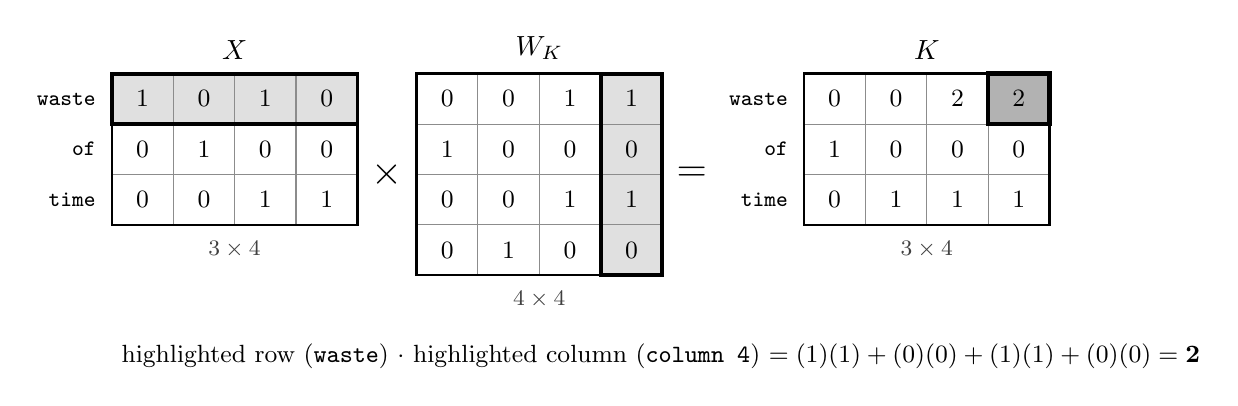
\begin{tikzpicture}
\draw[black!45, fill=black!12] (0.000,0.000) rectangle (0.780,-0.640);
\node[font=\small, text=black] at (0.390,-0.320) {$1$};
\draw[black!45, fill=black!12] (0.780,0.000) rectangle (1.560,-0.640);
\node[font=\small, text=black] at (1.170,-0.320) {$0$};
\draw[black!45, fill=black!12] (1.560,0.000) rectangle (2.340,-0.640);
\node[font=\small, text=black] at (1.950,-0.320) {$1$};
\draw[black!45, fill=black!12] (2.340,0.000) rectangle (3.120,-0.640);
\node[font=\small, text=black] at (2.730,-0.320) {$0$};
\draw[black!45, fill=white] (0.000,-0.640) rectangle (0.780,-1.279);
\node[font=\small, text=black] at (0.390,-0.959) {$0$};
\draw[black!45, fill=white] (0.780,-0.640) rectangle (1.560,-1.279);
\node[font=\small, text=black] at (1.170,-0.959) {$1$};
\draw[black!45, fill=white] (1.560,-0.640) rectangle (2.340,-1.279);
\node[font=\small, text=black] at (1.950,-0.959) {$0$};
\draw[black!45, fill=white] (2.340,-0.640) rectangle (3.120,-1.279);
\node[font=\small, text=black] at (2.730,-0.959) {$0$};
\draw[black!45, fill=white] (0.000,-1.279) rectangle (0.780,-1.919);
\node[font=\small, text=black] at (0.390,-1.599) {$0$};
\draw[black!45, fill=white] (0.780,-1.279) rectangle (1.560,-1.919);
\node[font=\small, text=black] at (1.170,-1.599) {$0$};
\draw[black!45, fill=white] (1.560,-1.279) rectangle (2.340,-1.919);
\node[font=\small, text=black] at (1.950,-1.599) {$1$};
\draw[black!45, fill=white] (2.340,-1.279) rectangle (3.120,-1.919);
\node[font=\small, text=black] at (2.730,-1.599) {$1$};
\draw[line width=1.4pt] (0.000,0.000) rectangle (3.120,-0.640);
\draw[line width=0.9pt] (0.000,0.000) rectangle (3.120,-1.919);
\node[anchor=east, font=\footnotesize\ttfamily] at (-0.080,-0.320) {waste};
\node[anchor=east, font=\footnotesize\ttfamily] at (-0.080,-0.959) {of};
\node[anchor=east, font=\footnotesize\ttfamily] at (-0.080,-1.599) {time};
\node[anchor=south, font=\normalsize] at (1.560,0.050) {$X$};
\node[anchor=north, font=\footnotesize, text=black!75] at (1.560,-1.999) {$3\times4$};
\draw[black!45, fill=white] (3.870,0.000) rectangle (4.650,-0.640);
\node[font=\small, text=black] at (4.260,-0.320) {$0$};
\draw[black!45, fill=white] (4.650,0.000) rectangle (5.430,-0.640);
\node[font=\small, text=black] at (5.040,-0.320) {$0$};
\draw[black!45, fill=white] (5.430,0.000) rectangle (6.210,-0.640);
\node[font=\small, text=black] at (5.820,-0.320) {$1$};
\draw[black!45, fill=black!12] (6.210,0.000) rectangle (6.990,-0.640);
\node[font=\small, text=black] at (6.600,-0.320) {$1$};
\draw[black!45, fill=white] (3.870,-0.640) rectangle (4.650,-1.279);
\node[font=\small, text=black] at (4.260,-0.959) {$1$};
\draw[black!45, fill=white] (4.650,-0.640) rectangle (5.430,-1.279);
\node[font=\small, text=black] at (5.040,-0.959) {$0$};
\draw[black!45, fill=white] (5.430,-0.640) rectangle (6.210,-1.279);
\node[font=\small, text=black] at (5.820,-0.959) {$0$};
\draw[black!45, fill=black!12] (6.210,-0.640) rectangle (6.990,-1.279);
\node[font=\small, text=black] at (6.600,-0.959) {$0$};
\draw[black!45, fill=white] (3.870,-1.279) rectangle (4.650,-1.919);
\node[font=\small, text=black] at (4.260,-1.599) {$0$};
\draw[black!45, fill=white] (4.650,-1.279) rectangle (5.430,-1.919);
\node[font=\small, text=black] at (5.040,-1.599) {$0$};
\draw[black!45, fill=white] (5.430,-1.279) rectangle (6.210,-1.919);
\node[font=\small, text=black] at (5.820,-1.599) {$1$};
\draw[black!45, fill=black!12] (6.210,-1.279) rectangle (6.990,-1.919);
\node[font=\small, text=black] at (6.600,-1.599) {$1$};
\draw[black!45, fill=white] (3.870,-1.919) rectangle (4.650,-2.558);
\node[font=\small, text=black] at (4.260,-2.239) {$0$};
\draw[black!45, fill=white] (4.650,-1.919) rectangle (5.430,-2.558);
\node[font=\small, text=black] at (5.040,-2.239) {$1$};
\draw[black!45, fill=white] (5.430,-1.919) rectangle (6.210,-2.558);
\node[font=\small, text=black] at (5.820,-2.239) {$0$};
\draw[black!45, fill=black!12] (6.210,-1.919) rectangle (6.990,-2.558);
\node[font=\small, text=black] at (6.600,-2.239) {$0$};
\draw[line width=1.4pt] (6.210,0.000) rectangle (6.990,-2.558);
\draw[line width=0.9pt] (3.870,0.000) rectangle (6.990,-2.558);
\node[anchor=south, font=\normalsize] at (5.430,0.050) {$W_K$};
\node[anchor=north, font=\footnotesize, text=black!75] at (5.430,-2.638) {$4\times4$};
\draw[black!45, fill=white] (8.790,0.000) rectangle (9.570,-0.640);
\node[font=\small, text=black] at (9.180,-0.320) {$0$};
\draw[black!45, fill=white] (9.570,0.000) rectangle (10.350,-0.640);
\node[font=\small, text=black] at (9.960,-0.320) {$0$};
\draw[black!45, fill=white] (10.350,0.000) rectangle (11.130,-0.640);
\node[font=\small, text=black] at (10.740,-0.320) {$2$};
\draw[black!45, fill=black!30] (11.130,0.000) rectangle (11.910,-0.640);
\node[font=\small, text=black] at (11.520,-0.320) {$2$};
\draw[black!45, fill=white] (8.790,-0.640) rectangle (9.570,-1.279);
\node[font=\small, text=black] at (9.180,-0.959) {$1$};
\draw[black!45, fill=white] (9.570,-0.640) rectangle (10.350,-1.279);
\node[font=\small, text=black] at (9.960,-0.959) {$0$};
\draw[black!45, fill=white] (10.350,-0.640) rectangle (11.130,-1.279);
\node[font=\small, text=black] at (10.740,-0.959) {$0$};
\draw[black!45, fill=white] (11.130,-0.640) rectangle (11.910,-1.279);
\node[font=\small, text=black] at (11.520,-0.959) {$0$};
\draw[black!45, fill=white] (8.790,-1.279) rectangle (9.570,-1.919);
\node[font=\small, text=black] at (9.180,-1.599) {$0$};
\draw[black!45, fill=white] (9.570,-1.279) rectangle (10.350,-1.919);
\node[font=\small, text=black] at (9.960,-1.599) {$1$};
\draw[black!45, fill=white] (10.350,-1.279) rectangle (11.130,-1.919);
\node[font=\small, text=black] at (10.740,-1.599) {$1$};
\draw[black!45, fill=white] (11.130,-1.279) rectangle (11.910,-1.919);
\node[font=\small, text=black] at (11.520,-1.599) {$1$};
\draw[line width=1.6pt] (11.130,0.000) rectangle (11.910,-0.640);
\draw[line width=0.9pt] (8.790,0.000) rectangle (11.910,-1.919);
\node[anchor=east, font=\footnotesize\ttfamily] at (8.710,-0.320) {waste};
\node[anchor=east, font=\footnotesize\ttfamily] at (8.710,-0.959) {of};
\node[anchor=east, font=\footnotesize\ttfamily] at (8.710,-1.599) {time};
\node[anchor=south, font=\normalsize] at (10.350,0.050) {$K$};
\node[anchor=north, font=\footnotesize, text=black!75] at (10.350,-1.999) {$3\times4$};
\node[font=\Large] at (3.495,-1.279) {$\times$};
\node[font=\Large] at (7.365,-1.279) {$=$};
\node[anchor=north west, font=\small, align=left] at (0,-3.308) {highlighted row (\texttt{waste}) $\cdot$ highlighted column (\texttt{column 4}) $= (1)(1) + (0)(0) + (1)(1) + (0)(0) = \mathbf{2}$};
\end{tikzpicture}
\\[10pt]
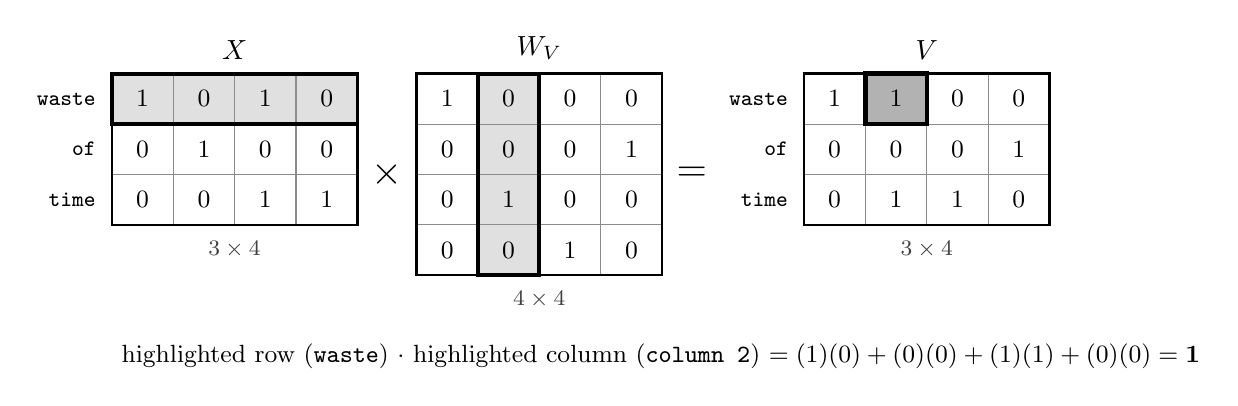
\begin{tikzpicture}
\draw[black!45, fill=black!12] (0.000,0.000) rectangle (0.780,-0.640);
\node[font=\small, text=black] at (0.390,-0.320) {$1$};
\draw[black!45, fill=black!12] (0.780,0.000) rectangle (1.560,-0.640);
\node[font=\small, text=black] at (1.170,-0.320) {$0$};
\draw[black!45, fill=black!12] (1.560,0.000) rectangle (2.340,-0.640);
\node[font=\small, text=black] at (1.950,-0.320) {$1$};
\draw[black!45, fill=black!12] (2.340,0.000) rectangle (3.120,-0.640);
\node[font=\small, text=black] at (2.730,-0.320) {$0$};
\draw[black!45, fill=white] (0.000,-0.640) rectangle (0.780,-1.279);
\node[font=\small, text=black] at (0.390,-0.959) {$0$};
\draw[black!45, fill=white] (0.780,-0.640) rectangle (1.560,-1.279);
\node[font=\small, text=black] at (1.170,-0.959) {$1$};
\draw[black!45, fill=white] (1.560,-0.640) rectangle (2.340,-1.279);
\node[font=\small, text=black] at (1.950,-0.959) {$0$};
\draw[black!45, fill=white] (2.340,-0.640) rectangle (3.120,-1.279);
\node[font=\small, text=black] at (2.730,-0.959) {$0$};
\draw[black!45, fill=white] (0.000,-1.279) rectangle (0.780,-1.919);
\node[font=\small, text=black] at (0.390,-1.599) {$0$};
\draw[black!45, fill=white] (0.780,-1.279) rectangle (1.560,-1.919);
\node[font=\small, text=black] at (1.170,-1.599) {$0$};
\draw[black!45, fill=white] (1.560,-1.279) rectangle (2.340,-1.919);
\node[font=\small, text=black] at (1.950,-1.599) {$1$};
\draw[black!45, fill=white] (2.340,-1.279) rectangle (3.120,-1.919);
\node[font=\small, text=black] at (2.730,-1.599) {$1$};
\draw[line width=1.4pt] (0.000,0.000) rectangle (3.120,-0.640);
\draw[line width=0.9pt] (0.000,0.000) rectangle (3.120,-1.919);
\node[anchor=east, font=\footnotesize\ttfamily] at (-0.080,-0.320) {waste};
\node[anchor=east, font=\footnotesize\ttfamily] at (-0.080,-0.959) {of};
\node[anchor=east, font=\footnotesize\ttfamily] at (-0.080,-1.599) {time};
\node[anchor=south, font=\normalsize] at (1.560,0.050) {$X$};
\node[anchor=north, font=\footnotesize, text=black!75] at (1.560,-1.999) {$3\times4$};
\draw[black!45, fill=white] (3.870,0.000) rectangle (4.650,-0.640);
\node[font=\small, text=black] at (4.260,-0.320) {$1$};
\draw[black!45, fill=black!12] (4.650,0.000) rectangle (5.430,-0.640);
\node[font=\small, text=black] at (5.040,-0.320) {$0$};
\draw[black!45, fill=white] (5.430,0.000) rectangle (6.210,-0.640);
\node[font=\small, text=black] at (5.820,-0.320) {$0$};
\draw[black!45, fill=white] (6.210,0.000) rectangle (6.990,-0.640);
\node[font=\small, text=black] at (6.600,-0.320) {$0$};
\draw[black!45, fill=white] (3.870,-0.640) rectangle (4.650,-1.279);
\node[font=\small, text=black] at (4.260,-0.959) {$0$};
\draw[black!45, fill=black!12] (4.650,-0.640) rectangle (5.430,-1.279);
\node[font=\small, text=black] at (5.040,-0.959) {$0$};
\draw[black!45, fill=white] (5.430,-0.640) rectangle (6.210,-1.279);
\node[font=\small, text=black] at (5.820,-0.959) {$0$};
\draw[black!45, fill=white] (6.210,-0.640) rectangle (6.990,-1.279);
\node[font=\small, text=black] at (6.600,-0.959) {$1$};
\draw[black!45, fill=white] (3.870,-1.279) rectangle (4.650,-1.919);
\node[font=\small, text=black] at (4.260,-1.599) {$0$};
\draw[black!45, fill=black!12] (4.650,-1.279) rectangle (5.430,-1.919);
\node[font=\small, text=black] at (5.040,-1.599) {$1$};
\draw[black!45, fill=white] (5.430,-1.279) rectangle (6.210,-1.919);
\node[font=\small, text=black] at (5.820,-1.599) {$0$};
\draw[black!45, fill=white] (6.210,-1.279) rectangle (6.990,-1.919);
\node[font=\small, text=black] at (6.600,-1.599) {$0$};
\draw[black!45, fill=white] (3.870,-1.919) rectangle (4.650,-2.558);
\node[font=\small, text=black] at (4.260,-2.239) {$0$};
\draw[black!45, fill=black!12] (4.650,-1.919) rectangle (5.430,-2.558);
\node[font=\small, text=black] at (5.040,-2.239) {$0$};
\draw[black!45, fill=white] (5.430,-1.919) rectangle (6.210,-2.558);
\node[font=\small, text=black] at (5.820,-2.239) {$1$};
\draw[black!45, fill=white] (6.210,-1.919) rectangle (6.990,-2.558);
\node[font=\small, text=black] at (6.600,-2.239) {$0$};
\draw[line width=1.4pt] (4.650,0.000) rectangle (5.430,-2.558);
\draw[line width=0.9pt] (3.870,0.000) rectangle (6.990,-2.558);
\node[anchor=south, font=\normalsize] at (5.430,0.050) {$W_V$};
\node[anchor=north, font=\footnotesize, text=black!75] at (5.430,-2.638) {$4\times4$};
\draw[black!45, fill=white] (8.790,0.000) rectangle (9.570,-0.640);
\node[font=\small, text=black] at (9.180,-0.320) {$1$};
\draw[black!45, fill=black!30] (9.570,0.000) rectangle (10.350,-0.640);
\node[font=\small, text=black] at (9.960,-0.320) {$1$};
\draw[black!45, fill=white] (10.350,0.000) rectangle (11.130,-0.640);
\node[font=\small, text=black] at (10.740,-0.320) {$0$};
\draw[black!45, fill=white] (11.130,0.000) rectangle (11.910,-0.640);
\node[font=\small, text=black] at (11.520,-0.320) {$0$};
\draw[black!45, fill=white] (8.790,-0.640) rectangle (9.570,-1.279);
\node[font=\small, text=black] at (9.180,-0.959) {$0$};
\draw[black!45, fill=white] (9.570,-0.640) rectangle (10.350,-1.279);
\node[font=\small, text=black] at (9.960,-0.959) {$0$};
\draw[black!45, fill=white] (10.350,-0.640) rectangle (11.130,-1.279);
\node[font=\small, text=black] at (10.740,-0.959) {$0$};
\draw[black!45, fill=white] (11.130,-0.640) rectangle (11.910,-1.279);
\node[font=\small, text=black] at (11.520,-0.959) {$1$};
\draw[black!45, fill=white] (8.790,-1.279) rectangle (9.570,-1.919);
\node[font=\small, text=black] at (9.180,-1.599) {$0$};
\draw[black!45, fill=white] (9.570,-1.279) rectangle (10.350,-1.919);
\node[font=\small, text=black] at (9.960,-1.599) {$1$};
\draw[black!45, fill=white] (10.350,-1.279) rectangle (11.130,-1.919);
\node[font=\small, text=black] at (10.740,-1.599) {$1$};
\draw[black!45, fill=white] (11.130,-1.279) rectangle (11.910,-1.919);
\node[font=\small, text=black] at (11.520,-1.599) {$0$};
\draw[line width=1.6pt] (9.570,0.000) rectangle (10.350,-0.640);
\draw[line width=0.9pt] (8.790,0.000) rectangle (11.910,-1.919);
\node[anchor=east, font=\footnotesize\ttfamily] at (8.710,-0.320) {waste};
\node[anchor=east, font=\footnotesize\ttfamily] at (8.710,-0.959) {of};
\node[anchor=east, font=\footnotesize\ttfamily] at (8.710,-1.599) {time};
\node[anchor=south, font=\normalsize] at (10.350,0.050) {$V$};
\node[anchor=north, font=\footnotesize, text=black!75] at (10.350,-1.999) {$3\times4$};
\node[font=\Large] at (3.495,-1.279) {$\times$};
\node[font=\Large] at (7.365,-1.279) {$=$};
\node[anchor=north west, font=\small, align=left] at (0,-3.308) {highlighted row (\texttt{waste}) $\cdot$ highlighted column (\texttt{column 2}) $= (1)(0) + (0)(0) + (1)(1) + (0)(0) = \mathbf{1}$};
\end{tikzpicture}

\caption{The three machines applied to the whole sentence: $Q=XW_Q$, $K=XW_K$, $V=XW_V$, each of shape
$T\times d_k=3\times4$. $W_Q$ is the identity in the toy, so $Q=X$; $W_K$ and $W_V$ move the arrows.}
\label{fig:qkv}
\end{figure}

\begin{checkq}
Why does attention give each token three arrows instead of one?
\begin{options}
\item It does not need to: the three are copies, and one would do.
\item What a token looks for, what it can be found by and what it hands over are different jobs, so each gets its own machine.
\item The values must keep the original meaning, so they cannot be shared with queries.
\item Only the current token needs a query; keys and values are for the other tokens.
\end{options}
\end{checkq}

\Summary{Each token gets a query (what it looks for), a key (what it is found by) and a value (what it hands over),
each from its own learned machine.}

%---------------------------------------------------------------------
\subsection*{3.6\quad Worked example: what does \tok{time} attend to?}

\Predict Look at $Q$ and $K$ above. Which earlier token do you expect \tok{time} to attend to most, and roughly
what share? Write it down before reading on.

\textbf{Step 1: match (every handshake at once).} $S = QK^\top$: every row of $Q$ meets every column of $K^\top$.
The highlighted row \tok{time} meeting the highlighted column \tok{waste} gives the cell circled in $S$.

\begin{figure}[!htb]
\centering
% AUTO-GENERATED by code/figlib.py helpers -- do not edit
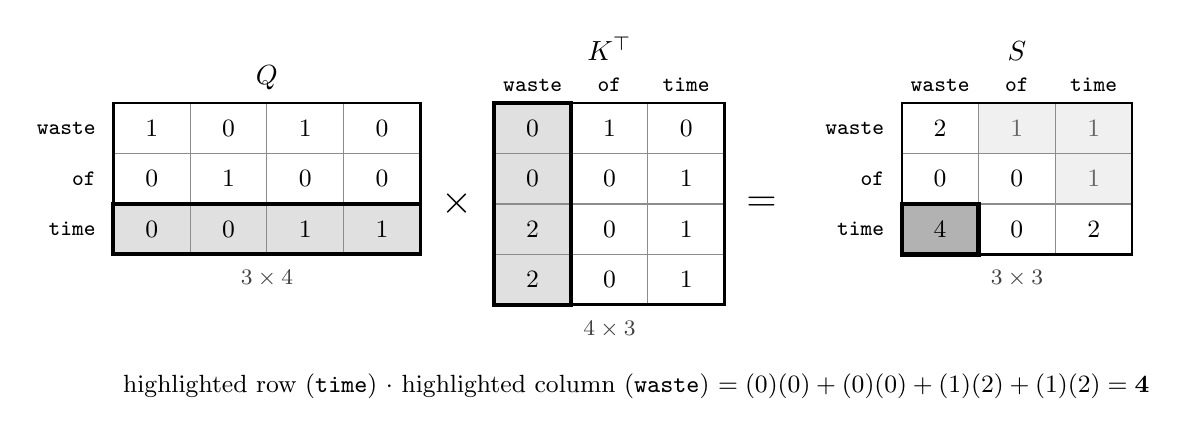
\begin{tikzpicture}[x=1.25cm]
\draw[black!45, fill=white] (0.000,0.000) rectangle (0.780,-0.640);
\node[font=\small, text=black] at (0.390,-0.320) {$1$};
\draw[black!45, fill=white] (0.780,0.000) rectangle (1.560,-0.640);
\node[font=\small, text=black] at (1.170,-0.320) {$0$};
\draw[black!45, fill=white] (1.560,0.000) rectangle (2.340,-0.640);
\node[font=\small, text=black] at (1.950,-0.320) {$1$};
\draw[black!45, fill=white] (2.340,0.000) rectangle (3.120,-0.640);
\node[font=\small, text=black] at (2.730,-0.320) {$0$};
\draw[black!45, fill=white] (0.000,-0.640) rectangle (0.780,-1.279);
\node[font=\small, text=black] at (0.390,-0.959) {$0$};
\draw[black!45, fill=white] (0.780,-0.640) rectangle (1.560,-1.279);
\node[font=\small, text=black] at (1.170,-0.959) {$1$};
\draw[black!45, fill=white] (1.560,-0.640) rectangle (2.340,-1.279);
\node[font=\small, text=black] at (1.950,-0.959) {$0$};
\draw[black!45, fill=white] (2.340,-0.640) rectangle (3.120,-1.279);
\node[font=\small, text=black] at (2.730,-0.959) {$0$};
\draw[black!45, fill=black!12] (0.000,-1.279) rectangle (0.780,-1.919);
\node[font=\small, text=black] at (0.390,-1.599) {$0$};
\draw[black!45, fill=black!12] (0.780,-1.279) rectangle (1.560,-1.919);
\node[font=\small, text=black] at (1.170,-1.599) {$0$};
\draw[black!45, fill=black!12] (1.560,-1.279) rectangle (2.340,-1.919);
\node[font=\small, text=black] at (1.950,-1.599) {$1$};
\draw[black!45, fill=black!12] (2.340,-1.279) rectangle (3.120,-1.919);
\node[font=\small, text=black] at (2.730,-1.599) {$1$};
\draw[line width=1.4pt] (0.000,-1.279) rectangle (3.120,-1.919);
\draw[line width=0.9pt] (0.000,0.000) rectangle (3.120,-1.919);
\node[anchor=east, font=\footnotesize\ttfamily] at (-0.080,-0.320) {waste};
\node[anchor=east, font=\footnotesize\ttfamily] at (-0.080,-0.959) {of};
\node[anchor=east, font=\footnotesize\ttfamily] at (-0.080,-1.599) {time};
\node[anchor=south, font=\normalsize] at (1.560,0.050) {$Q$};
\node[anchor=north, font=\footnotesize, text=black!75] at (1.560,-1.999) {$3\times4$};
\draw[black!45, fill=black!12] (3.870,0.000) rectangle (4.650,-0.640);
\node[font=\small, text=black] at (4.260,-0.320) {$0$};
\draw[black!45, fill=white] (4.650,0.000) rectangle (5.430,-0.640);
\node[font=\small, text=black] at (5.040,-0.320) {$1$};
\draw[black!45, fill=white] (5.430,0.000) rectangle (6.210,-0.640);
\node[font=\small, text=black] at (5.820,-0.320) {$0$};
\draw[black!45, fill=black!12] (3.870,-0.640) rectangle (4.650,-1.279);
\node[font=\small, text=black] at (4.260,-0.959) {$0$};
\draw[black!45, fill=white] (4.650,-0.640) rectangle (5.430,-1.279);
\node[font=\small, text=black] at (5.040,-0.959) {$0$};
\draw[black!45, fill=white] (5.430,-0.640) rectangle (6.210,-1.279);
\node[font=\small, text=black] at (5.820,-0.959) {$1$};
\draw[black!45, fill=black!12] (3.870,-1.279) rectangle (4.650,-1.919);
\node[font=\small, text=black] at (4.260,-1.599) {$2$};
\draw[black!45, fill=white] (4.650,-1.279) rectangle (5.430,-1.919);
\node[font=\small, text=black] at (5.040,-1.599) {$0$};
\draw[black!45, fill=white] (5.430,-1.279) rectangle (6.210,-1.919);
\node[font=\small, text=black] at (5.820,-1.599) {$1$};
\draw[black!45, fill=black!12] (3.870,-1.919) rectangle (4.650,-2.558);
\node[font=\small, text=black] at (4.260,-2.239) {$2$};
\draw[black!45, fill=white] (4.650,-1.919) rectangle (5.430,-2.558);
\node[font=\small, text=black] at (5.040,-2.239) {$0$};
\draw[black!45, fill=white] (5.430,-1.919) rectangle (6.210,-2.558);
\node[font=\small, text=black] at (5.820,-2.239) {$1$};
\draw[line width=1.4pt] (3.870,0.000) rectangle (4.650,-2.558);
\draw[line width=0.9pt] (3.870,0.000) rectangle (6.210,-2.558);
\node[anchor=south, font=\footnotesize\ttfamily] at (4.260,0.020) {waste};
\node[anchor=south, font=\footnotesize\ttfamily] at (5.040,0.020) {of};
\node[anchor=south, font=\footnotesize\ttfamily] at (5.820,0.020) {time};
\node[anchor=south, font=\normalsize] at (5.040,0.420) {$K^{\top}$};
\node[anchor=north, font=\footnotesize, text=black!75] at (5.040,-2.638) {$4\times3$};
\draw[black!45, fill=white] (8.010,0.000) rectangle (8.790,-0.640);
\node[font=\small, text=black] at (8.400,-0.320) {$2$};
\draw[black!45, fill=black!6] (8.790,0.000) rectangle (9.570,-0.640);
\node[font=\small, text=black!60] at (9.180,-0.320) {$1$};
\draw[black!45, fill=black!6] (9.570,0.000) rectangle (10.350,-0.640);
\node[font=\small, text=black!60] at (9.960,-0.320) {$1$};
\draw[black!45, fill=white] (8.010,-0.640) rectangle (8.790,-1.279);
\node[font=\small, text=black] at (8.400,-0.959) {$0$};
\draw[black!45, fill=white] (8.790,-0.640) rectangle (9.570,-1.279);
\node[font=\small, text=black] at (9.180,-0.959) {$0$};
\draw[black!45, fill=black!6] (9.570,-0.640) rectangle (10.350,-1.279);
\node[font=\small, text=black!60] at (9.960,-0.959) {$1$};
\draw[black!45, fill=black!30] (8.010,-1.279) rectangle (8.790,-1.919);
\node[font=\small, text=black] at (8.400,-1.599) {$4$};
\draw[black!45, fill=white] (8.790,-1.279) rectangle (9.570,-1.919);
\node[font=\small, text=black] at (9.180,-1.599) {$0$};
\draw[black!45, fill=white] (9.570,-1.279) rectangle (10.350,-1.919);
\node[font=\small, text=black] at (9.960,-1.599) {$2$};
\draw[line width=1.6pt] (8.010,-1.279) rectangle (8.790,-1.919);
\draw[line width=0.9pt] (8.010,0.000) rectangle (10.350,-1.919);
\node[anchor=east, font=\footnotesize\ttfamily] at (7.930,-0.320) {waste};
\node[anchor=east, font=\footnotesize\ttfamily] at (7.930,-0.959) {of};
\node[anchor=east, font=\footnotesize\ttfamily] at (7.930,-1.599) {time};
\node[anchor=south, font=\footnotesize\ttfamily] at (8.400,0.020) {waste};
\node[anchor=south, font=\footnotesize\ttfamily] at (9.180,0.020) {of};
\node[anchor=south, font=\footnotesize\ttfamily] at (9.960,0.020) {time};
\node[anchor=south, font=\normalsize] at (9.180,0.420) {$S$};
\node[anchor=north, font=\footnotesize, text=black!75] at (9.180,-1.999) {$3\times3$};
\node[font=\Large] at (3.495,-1.279) {$\times$};
\node[font=\Large] at (6.585,-1.279) {$=$};
\node[anchor=north west, font=\small, align=left] at (0,-3.308) {highlighted row (\texttt{time}) $\cdot$ highlighted column (\texttt{waste}) $= (0)(0) + (0)(0) + (1)(2) + (1)(2) = \mathbf{4}$};
\end{tikzpicture}

\caption{$S=QK^\top$ for our sentence, $(3\times4)(4\times3)=3\times3$. Row \tok{time} reads $(\sWaste, \sOf,
\sTime)$. Grey cells are a token meeting a token that comes \emph{after} it; Step 3 removes them.}
\end{figure}

Look at row \tok{time} through the geometry of \S3.2. Its query is $\bm{q}_{\text{time}}=(0,0,1,1)$, of length
\lenQ. Each score is length $\times$ length $\times$ agreement:

\begin{center}
\small
\begin{tabular}{@{}l c c c c c@{}}
\toprule
key & $\lVert\bm{k}\rVert$ & angle to $\bm{q}_{\text{time}}$ & $\cos\theta$ & $\lVert\bm{q}\rVert\lVert\bm{k}\rVert\cos\theta$ & dot product\\
\midrule
\tok{waste} & \lenWaste & \angWaste$^\circ$ & \cosWaste & \sWaste & \sWaste\\
\tok{of} & \lenOf & \angOf$^\circ$ & \cosOf & \sOf & \sOf\\
\tok{time} & \lenTime & \angTime$^\circ$ & \cosTime & \sTime & \sTime\\
\bottomrule
\end{tabular}
\end{center}
\tok{time}'s question points \emph{exactly} along \tok{waste}'s label (0 degrees), at right angles to \tok{of}'s
(nothing in common), and partly along its own. That is what ``\tok{waste} is relevant to \tok{time}'' means,
geometrically.

\textbf{Step 2: scale.} Divide by $\sqrt{d_k}=\sqrt4=2$. Row \tok{time} becomes $(\ssWaste, \ssOf, \ssTime)$. Why
we divide is the subject of \S3.8.

\textbf{Step 3: cover the answers.} Remember from \S1.9 that one sentence is three exercises: after \tok{waste},
guess the next word; after \tok{waste of}, guess the next; and so on. The exercise ``after \tok{waste of}, guess
the next word'' must not be allowed to see \tok{time}: that is the answer.

\Picture An exam where all the questions and all the answers are printed on one long sheet, in order. Before each
question, you cover everything below it with a ruler. A fraud-detection model is trained the same way: it may
never use information recorded \emph{after} the transaction, because in production that information does not
exist yet. A model that used it would look brilliant in training and fail in the real world.

\begin{breaks}
On the exam sheet you cover the answers once. Here every row has its own ruler at a different height, and all the
rulers are applied at the same moment.
\end{breaks}

\Exactly Set every score above the diagonal (the grey cells) to $-\infty$. This is \emph{causal masking}:
\begin{center}% AUTO-GENERATED by code/figlib.py helpers -- do not edit
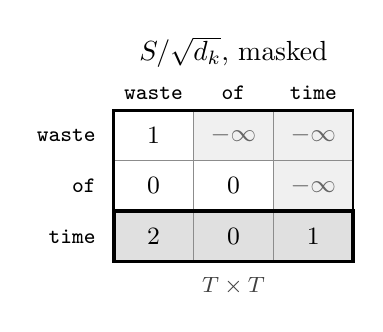
\begin{tikzpicture}[x=1.3cm]
\draw[black!45, fill=white] (0.000,0.000) rectangle (0.780,-0.640);
\node[font=\small, text=black] at (0.390,-0.320) {$1$};
\draw[black!45, fill=black!6] (0.780,0.000) rectangle (1.560,-0.640);
\node[font=\small, text=black!60] at (1.170,-0.320) {$-\infty$};
\draw[black!45, fill=black!6] (1.560,0.000) rectangle (2.340,-0.640);
\node[font=\small, text=black!60] at (1.950,-0.320) {$-\infty$};
\draw[black!45, fill=white] (0.000,-0.640) rectangle (0.780,-1.279);
\node[font=\small, text=black] at (0.390,-0.959) {$0$};
\draw[black!45, fill=white] (0.780,-0.640) rectangle (1.560,-1.279);
\node[font=\small, text=black] at (1.170,-0.959) {$0$};
\draw[black!45, fill=black!6] (1.560,-0.640) rectangle (2.340,-1.279);
\node[font=\small, text=black!60] at (1.950,-0.959) {$-\infty$};
\draw[black!45, fill=black!12] (0.000,-1.279) rectangle (0.780,-1.919);
\node[font=\small, text=black] at (0.390,-1.599) {$2$};
\draw[black!45, fill=black!12] (0.780,-1.279) rectangle (1.560,-1.919);
\node[font=\small, text=black] at (1.170,-1.599) {$0$};
\draw[black!45, fill=black!12] (1.560,-1.279) rectangle (2.340,-1.919);
\node[font=\small, text=black] at (1.950,-1.599) {$1$};
\draw[line width=1.4pt] (0.000,-1.279) rectangle (2.340,-1.919);
\draw[line width=0.9pt] (0.000,0.000) rectangle (2.340,-1.919);
\node[anchor=east, font=\footnotesize\ttfamily] at (-0.080,-0.320) {waste};
\node[anchor=east, font=\footnotesize\ttfamily] at (-0.080,-0.959) {of};
\node[anchor=east, font=\footnotesize\ttfamily] at (-0.080,-1.599) {time};
\node[anchor=south, font=\footnotesize\ttfamily] at (0.390,0.020) {waste};
\node[anchor=south, font=\footnotesize\ttfamily] at (1.170,0.020) {of};
\node[anchor=south, font=\footnotesize\ttfamily] at (1.950,0.020) {time};
\node[anchor=south, font=\normalsize] at (1.170,0.420) {$S/\sqrt{d_k}$, masked};
\node[anchor=north, font=\footnotesize, text=black!75] at (1.170,-1.999) {$T\times T$};
\end{tikzpicture}
\end{center}
Step 4 will turn $-\infty$ into a weight of exactly zero. So the row for \tok{of} is built only from \tok{waste}
and \tok{of}; our script checks that changing the arrow of \tok{time} to anything at all leaves the first two rows
of the output untouched. That is why the three exercises can be solved \emph{in the same pass} without cheating.

\begin{wrongidea}{3.7}
\emph{The mask exists only to stop cheating.} That is how it is usually introduced: without it, the model
could copy from the future tokens. That is true, and it is half the story. The other half
is speed: because each row ignores everything after it, one pass can train all $T$ positions at once. Without
the mask you would need $T$ separate passes, one per prefix.
\end{wrongidea}

\textbf{Step 4: turn scores into shares (softmax).} For each row: raise $e$ to each score, then divide by the
row's total. For \tok{time}, the three steps are the three rows of this table:
\begin{center}% AUTO-GENERATED by code/figlib.py helpers -- do not edit
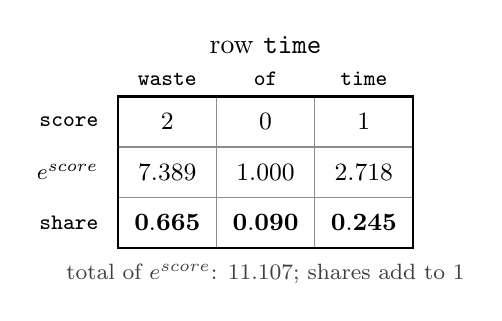
\begin{tikzpicture}[x=1.6cm]
\draw[black!45, fill=white] (0.000,0.000) rectangle (0.780,-0.640);
\node[font=\small, text=black] at (0.390,-0.320) {$2$};
\draw[black!45, fill=white] (0.780,0.000) rectangle (1.560,-0.640);
\node[font=\small, text=black] at (1.170,-0.320) {$0$};
\draw[black!45, fill=white] (1.560,0.000) rectangle (2.340,-0.640);
\node[font=\small, text=black] at (1.950,-0.320) {$1$};
\draw[black!45, fill=white] (0.000,-0.640) rectangle (0.780,-1.279);
\node[font=\small, text=black] at (0.390,-0.959) {$7.389$};
\draw[black!45, fill=white] (0.780,-0.640) rectangle (1.560,-1.279);
\node[font=\small, text=black] at (1.170,-0.959) {$1.000$};
\draw[black!45, fill=white] (1.560,-0.640) rectangle (2.340,-1.279);
\node[font=\small, text=black] at (1.950,-0.959) {$2.718$};
\draw[black!45, fill=white] (0.000,-1.279) rectangle (0.780,-1.919);
\node[font=\small, text=black] at (0.390,-1.599) {$\mathbf{0.665}$};
\draw[black!45, fill=white] (0.780,-1.279) rectangle (1.560,-1.919);
\node[font=\small, text=black] at (1.170,-1.599) {$\mathbf{0.090}$};
\draw[black!45, fill=white] (1.560,-1.279) rectangle (2.340,-1.919);
\node[font=\small, text=black] at (1.950,-1.599) {$\mathbf{0.245}$};
\draw[line width=0.9pt] (0.000,0.000) rectangle (2.340,-1.919);
\node[anchor=east, font=\footnotesize\ttfamily] at (-0.080,-0.320) {score};
\node[anchor=east, font=\footnotesize\ttfamily] at (-0.080,-0.959) {$e^{\text{score}}$};
\node[anchor=east, font=\footnotesize\ttfamily] at (-0.080,-1.599) {share};
\node[anchor=south, font=\footnotesize\ttfamily] at (0.390,0.020) {waste};
\node[anchor=south, font=\footnotesize\ttfamily] at (1.170,0.020) {of};
\node[anchor=south, font=\footnotesize\ttfamily] at (1.950,0.020) {time};
\node[anchor=south, font=\normalsize] at (1.170,0.420) {row \texttt{time}};
\node[anchor=north, font=\footnotesize, text=black!75] at (1.170,-1.999) {total of $e^{\text{score}}$: $11.107$; shares add to 1};
\end{tikzpicture}
\end{center}
In symbols, $\bm{a}_{\text{time}} = \left(\tfrac{\eWaste}{\eSum},\ \tfrac{\eOf}{\eSum},\ \tfrac{\eTime}{\eSum}\right)
= (\aWaste,\ \aOf,\ \aTime)$.
\tok{time} gives \apctWaste\% of its attention to \tok{waste}, \apctOf\% to \tok{of} and \apctTime\% to itself.
How close was your prediction? Compare that with the fixed 33.3\% each of \S3.1: the weights now come from the
content.

\Sanity The three shares are positive and add to 1, and the biggest score got the biggest share. A share above 1
or a negative share would mean an arithmetic slip.

\begin{wrongidea}{3.2}
\emph{Attention scores are already percentages.} They come out as one number per pair, like a table of shares, so
it is natural to read $(\sWaste,\sOf,\sTime)$ as ``4 parts to \tok{waste}''. No: scores can be negative and do not add to 1. Only after
softmax are they shares.
\end{wrongidea}

\begin{wrongidea}{3.5}
\emph{The current token only needs a query; keys and values are for the other tokens.} The current token is the
one asking, so its own key and value seem pointless.
Look at the result: \tok{time} gives \apctTime\% of its attention to \emph{itself}, through its own key and value.
And later tokens, such as \tok{Sorry}, will look back at \tok{time} through the same key and value.
\end{wrongidea}

\textbf{Step 5: collect.} The shares are shares \emph{of the values}, the contents of the books:
\[
\bm{o}_{\text{time}} = \aWaste\,\bm{v}_{\text{waste}} + \aOf\,\bm{v}_{\text{of}} + \aTime\,\bm{v}_{\text{time}}
= \oTime \shape{1\times d_k}
\]
and for the whole sentence at once, $O=AV$ ($T\times T$ times $T\times d_k$). The highlighted row of $A$ holds
\tok{time}'s shares; the highlighted column of $V$ holds the second number of each value arrow:
\begin{center}\resizebox{\linewidth}{!}{% AUTO-GENERATED by code/figlib.py helpers -- do not edit
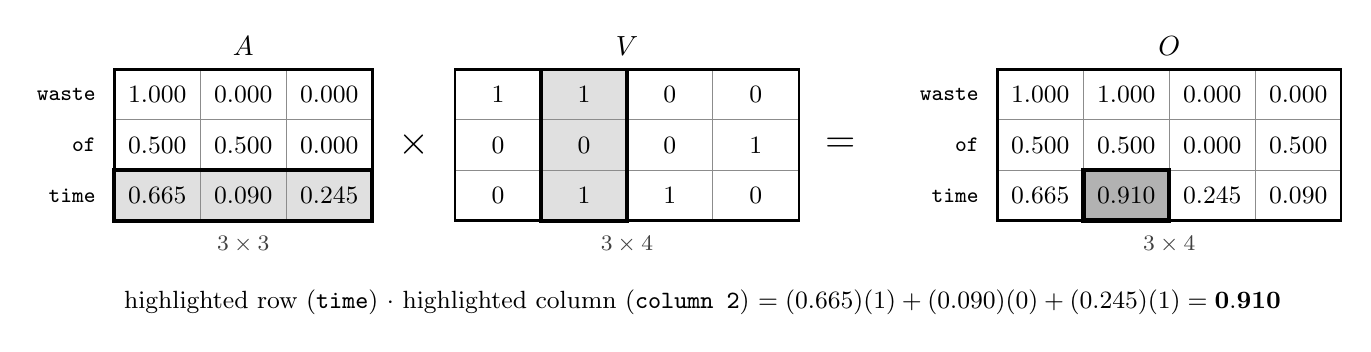
\begin{tikzpicture}[x=1.4cm]
\draw[black!45, fill=white] (0.000,0.000) rectangle (0.780,-0.640);
\node[font=\small, text=black] at (0.390,-0.320) {$1.000$};
\draw[black!45, fill=white] (0.780,0.000) rectangle (1.560,-0.640);
\node[font=\small, text=black] at (1.170,-0.320) {$0.000$};
\draw[black!45, fill=white] (1.560,0.000) rectangle (2.340,-0.640);
\node[font=\small, text=black] at (1.950,-0.320) {$0.000$};
\draw[black!45, fill=white] (0.000,-0.640) rectangle (0.780,-1.279);
\node[font=\small, text=black] at (0.390,-0.959) {$0.500$};
\draw[black!45, fill=white] (0.780,-0.640) rectangle (1.560,-1.279);
\node[font=\small, text=black] at (1.170,-0.959) {$0.500$};
\draw[black!45, fill=white] (1.560,-0.640) rectangle (2.340,-1.279);
\node[font=\small, text=black] at (1.950,-0.959) {$0.000$};
\draw[black!45, fill=black!12] (0.000,-1.279) rectangle (0.780,-1.919);
\node[font=\small, text=black] at (0.390,-1.599) {$0.665$};
\draw[black!45, fill=black!12] (0.780,-1.279) rectangle (1.560,-1.919);
\node[font=\small, text=black] at (1.170,-1.599) {$0.090$};
\draw[black!45, fill=black!12] (1.560,-1.279) rectangle (2.340,-1.919);
\node[font=\small, text=black] at (1.950,-1.599) {$0.245$};
\draw[line width=1.4pt] (0.000,-1.279) rectangle (2.340,-1.919);
\draw[line width=0.9pt] (0.000,0.000) rectangle (2.340,-1.919);
\node[anchor=east, font=\footnotesize\ttfamily] at (-0.080,-0.320) {waste};
\node[anchor=east, font=\footnotesize\ttfamily] at (-0.080,-0.959) {of};
\node[anchor=east, font=\footnotesize\ttfamily] at (-0.080,-1.599) {time};
\node[anchor=south, font=\normalsize] at (1.170,0.050) {$A$};
\node[anchor=north, font=\footnotesize, text=black!75] at (1.170,-1.999) {$3\times3$};
\draw[black!45, fill=white] (3.090,0.000) rectangle (3.870,-0.640);
\node[font=\small, text=black] at (3.480,-0.320) {$1$};
\draw[black!45, fill=black!12] (3.870,0.000) rectangle (4.650,-0.640);
\node[font=\small, text=black] at (4.260,-0.320) {$1$};
\draw[black!45, fill=white] (4.650,0.000) rectangle (5.430,-0.640);
\node[font=\small, text=black] at (5.040,-0.320) {$0$};
\draw[black!45, fill=white] (5.430,0.000) rectangle (6.210,-0.640);
\node[font=\small, text=black] at (5.820,-0.320) {$0$};
\draw[black!45, fill=white] (3.090,-0.640) rectangle (3.870,-1.279);
\node[font=\small, text=black] at (3.480,-0.959) {$0$};
\draw[black!45, fill=black!12] (3.870,-0.640) rectangle (4.650,-1.279);
\node[font=\small, text=black] at (4.260,-0.959) {$0$};
\draw[black!45, fill=white] (4.650,-0.640) rectangle (5.430,-1.279);
\node[font=\small, text=black] at (5.040,-0.959) {$0$};
\draw[black!45, fill=white] (5.430,-0.640) rectangle (6.210,-1.279);
\node[font=\small, text=black] at (5.820,-0.959) {$1$};
\draw[black!45, fill=white] (3.090,-1.279) rectangle (3.870,-1.919);
\node[font=\small, text=black] at (3.480,-1.599) {$0$};
\draw[black!45, fill=black!12] (3.870,-1.279) rectangle (4.650,-1.919);
\node[font=\small, text=black] at (4.260,-1.599) {$1$};
\draw[black!45, fill=white] (4.650,-1.279) rectangle (5.430,-1.919);
\node[font=\small, text=black] at (5.040,-1.599) {$1$};
\draw[black!45, fill=white] (5.430,-1.279) rectangle (6.210,-1.919);
\node[font=\small, text=black] at (5.820,-1.599) {$0$};
\draw[line width=1.4pt] (3.870,0.000) rectangle (4.650,-1.919);
\draw[line width=0.9pt] (3.090,0.000) rectangle (6.210,-1.919);
\node[anchor=south, font=\normalsize] at (4.650,0.050) {$V$};
\node[anchor=north, font=\footnotesize, text=black!75] at (4.650,-1.999) {$3\times4$};
\draw[black!45, fill=white] (8.010,0.000) rectangle (8.790,-0.640);
\node[font=\small, text=black] at (8.400,-0.320) {$1.000$};
\draw[black!45, fill=white] (8.790,0.000) rectangle (9.570,-0.640);
\node[font=\small, text=black] at (9.180,-0.320) {$1.000$};
\draw[black!45, fill=white] (9.570,0.000) rectangle (10.350,-0.640);
\node[font=\small, text=black] at (9.960,-0.320) {$0.000$};
\draw[black!45, fill=white] (10.350,0.000) rectangle (11.130,-0.640);
\node[font=\small, text=black] at (10.740,-0.320) {$0.000$};
\draw[black!45, fill=white] (8.010,-0.640) rectangle (8.790,-1.279);
\node[font=\small, text=black] at (8.400,-0.959) {$0.500$};
\draw[black!45, fill=white] (8.790,-0.640) rectangle (9.570,-1.279);
\node[font=\small, text=black] at (9.180,-0.959) {$0.500$};
\draw[black!45, fill=white] (9.570,-0.640) rectangle (10.350,-1.279);
\node[font=\small, text=black] at (9.960,-0.959) {$0.000$};
\draw[black!45, fill=white] (10.350,-0.640) rectangle (11.130,-1.279);
\node[font=\small, text=black] at (10.740,-0.959) {$0.500$};
\draw[black!45, fill=white] (8.010,-1.279) rectangle (8.790,-1.919);
\node[font=\small, text=black] at (8.400,-1.599) {$0.665$};
\draw[black!45, fill=black!30] (8.790,-1.279) rectangle (9.570,-1.919);
\node[font=\small, text=black] at (9.180,-1.599) {$0.910$};
\draw[black!45, fill=white] (9.570,-1.279) rectangle (10.350,-1.919);
\node[font=\small, text=black] at (9.960,-1.599) {$0.245$};
\draw[black!45, fill=white] (10.350,-1.279) rectangle (11.130,-1.919);
\node[font=\small, text=black] at (10.740,-1.599) {$0.090$};
\draw[line width=1.6pt] (8.790,-1.279) rectangle (9.570,-1.919);
\draw[line width=0.9pt] (8.010,0.000) rectangle (11.130,-1.919);
\node[anchor=east, font=\footnotesize\ttfamily] at (7.930,-0.320) {waste};
\node[anchor=east, font=\footnotesize\ttfamily] at (7.930,-0.959) {of};
\node[anchor=east, font=\footnotesize\ttfamily] at (7.930,-1.599) {time};
\node[anchor=south, font=\normalsize] at (9.570,0.050) {$O$};
\node[anchor=north, font=\footnotesize, text=black!75] at (9.570,-1.999) {$3\times4$};
\node[font=\Large] at (2.715,-0.959) {$\times$};
\node[font=\Large] at (6.585,-0.959) {$=$};
\node[anchor=north west, font=\small, align=left] at (0,-2.669) {highlighted row (\texttt{time}) $\cdot$ highlighted column (\texttt{column 2}) $= (0.665)(1) + (0.090)(0) + (0.245)(1) = \mathbf{0.910}$};
\end{tikzpicture}
}\end{center}
Every row of $O$ is a blend of value arrows, mixed in the proportions the token asked for. The arrow of \tok{time}
that leaves this step is no longer ``time in general''; it carries \apctWaste\% of what \tok{waste} had to say.

\begin{figure}[h]
\centering
\begin{tikzpicture}[x=0.47cm,y=0.47cm,font=\footnotesize]
\newcommand{\panel}[6]{%
  \begin{scope}[shift={(#1,0)}]
  \draw[gray!60] (-0.4,0)--(6.4,0);
  \fill[black!70] (0,0) rectangle (1.6,#3*#6);
  \fill[black!35] (2.2,0) rectangle (3.8,#4*#6);
  \fill[black!55] (4.4,0) rectangle (6.0,#5*#6);
  \node[above] at (0.8,#3*#6) {#3}; \node[above] at (3.0,#4*#6) {#4}; \node[above] at (5.2,#5*#6) {#5};
  \node at (3,-0.9) {#2};
  \end{scope}}
\panel{0}{1. match $S$}{\sWaste}{\sOf}{\sTime}{0.9}
\panel{9}{2. scale $\div\sqrt{d_k}$}{\ssWaste}{\ssOf}{\ssTime}{0.9}
\panel{18}{3--4a. exponentiate}{\eWaste}{\eOf}{\eTime}{0.5}
\panel{27}{4b. normalise}{\aWaste}{\aOf}{\aTime}{5}
\foreach \x in {7.3,16.3,25.3} \draw[-{Stealth},black!70, line width=0.8pt] (\x,2)--(\x+1.2,2);
\end{tikzpicture}
\caption{The frames of attention for the query \tok{time}. Bars: \tok{waste}, \tok{of}, \tok{time}. In the web
edition this strip is an animation you can scrub and re-run with your own weights.}
\end{figure}

\begin{checkq}
After masking, why can the three next-word exercises of \tok{waste of time} be trained in a single pass?
\begin{options}
\item The mask only stops cheating; it has nothing to do with doing them together.
\item Each row's output depends only on that token and earlier ones, so every row is an honest answer to its own exercise.
\item The raw scores are already percentages, so no extra step is needed per row.
\item Because \tok{time} gives no attention to itself.
\end{options}
\end{checkq}

\Summary{Match queries with keys, scale, mask the future, turn scores into shares, and blend the values: \tok{time}
ends up carrying \apctWaste\% of \tok{waste}.}

%---------------------------------------------------------------------
\subsection*{3.7\quad Why softmax, and not ``divide by the total''?}

\Picture A pizza is shared among friends according to votes. Softmax is the sharing rule.

\begin{breaks}
Votes are never negative, but scores can be. And the pizza rule we are about to build rewards a clear winner far
more than a fair-minded host would.
\end{breaks}

Three properties make $e^{\text{score}}$ the right rule, and each one is a requirement you could have written
down yourself:
\begin{enumerate}[label=(\roman*)]
\item \emph{Shares must be positive}, but scores can be negative (arrows pointing apart). $e^{s}$ is positive for
every $s$, and $e^{-\infty}=0$, which is what the mask needs.
\item \emph{Only differences should matter.} If every friend's vote goes up by 10, nobody deserves more pizza.
Indeed $e^{s+10}=e^{10}e^{s}$, and the common factor $e^{10}$ cancels in the division; our script confirms that
$(\ssWaste,\ssOf,\ssTime)$ and the same scores plus 10 give identical shares.
\item \emph{Leaders should lead.} Each extra point of score multiplies a share's weight by $e\approx2.718$, so a
clear winner gets a clear majority instead of a narrow one.
\end{enumerate}

\Predict Keep \tok{time}'s query pointing the same way but make it twice as long. Will the share for \tok{waste}
go up, go down, or stay at \aWaste?

Its scaled scores become $\dblScores$ and the shares become $(\dblWaste, \dblOf, \dblTime)$: same ranking, much
more decisive. \emph{The direction of a query decides what it looks for; its length decides how sure it is.}

\begin{wrongidea}{3.11}
\emph{Softmax shares depend on the ratios between scores, as when dividing by the total.} That is how percentages
are usually made, so it is the first rule anyone tries. Dividing by the total would give
$(\nThreeRatioA)$ for $(2,0,1)$ and $(\nThreeRatioB)$ for $(7,5,6)$: the shares would change when every score moves up by the same
amount. Softmax gives $(\nThreeSoft)$ for both, because of property (ii).
\end{wrongidea}

\begin{checkq}
After scaling, \tok{time}'s scores are $(2, 0, 1)$. Add 5 to all three, giving $(7, 5, 6)$, and apply softmax. What
happens to the shares? Then pick the reason.
\begin{options}
\item They do not change.
\item They all grow, because every score grew.
\item They become more even, since 7, 5 and 6 are closer together relative to their size.
\item \tok{waste}'s share grows most, because it had the largest score.
\end{options}
\emph{Reason:} (i) softmax only sees differences between scores; (ii) shares must still add to 1; (iii) $e^x$
grows faster for bigger $x$.
\end{checkq}

\Summary{Softmax makes shares that are positive, ignore a common shift, and favour the leader, and a longer query
makes it more decisive.}

%---------------------------------------------------------------------
\subsection*{3.8\quad Why divide by $\sqrt{d_k}$?}

In the toy the division looks cosmetic. It is not.

\Picture Toss a coin $d_k$ times; step forward on heads, back on tails. After 4 tosses you are usually within
about 2 steps of the start; after 1024 tosses, usually within about 32. The more tosses, the further you wander,
but not $d_k$ steps: about $\sqrt{d_k}$.

\begin{breaks}
Coin tosses are exactly $+1$ or $-1$. The products inside a dot product take any size; the $\sqrt{d_k}$ rule still
holds when each product has mean 0 and variance 1, which is how weights start out.
\end{breaks}

\Predict At $d_k=1024$, with no scaling, what share do you expect the top key to get out of 8 random keys, before
any training? Closer to $1/8$, to $1/2$, or to 1?

\Exactly A dot product of two unrelated arrows is a sum of $d_k$ products that are equally likely to be positive or
negative, like those coin tosses. If each coordinate has mean 0 and variance 1, the sum has variance $d_k$, so its
typical size is $\sqrt{d_k}$. We measured it (random queries against 8 random keys, 4000 trials, fixed seed):

\begin{center}
\small
\begin{tabular}{@{}r r r r@{}}
\toprule
$d_k$ & spread of $\bm{q}\cdot\bm{k}$ (theory $\sqrt{d_k}$) & largest share, unscaled & largest share, scaled\\
\midrule
4 & \sdFour\ (\sqrtFour) & \mxRawFour & \mxScFour\\
64 & \sdSixtyFour\ (\sqrtSixtyFour) & \mxRawSixtyFour & \mxScSixtyFour\\
1024 & \sdThousand\ (\sqrtThousand) & \mxRawThousand & \mxScThousand\\
\bottomrule
\end{tabular}
\end{center}

Read the third column with property (iii) of softmax in mind. At the widths real models use, random scores are tens
of points apart, so softmax hands almost everything to one key (\mxRawThousand\ on average at $d_k=1024$)
\emph{before the model has learned anything}. It has made up its mind at random, and, as Chapter 8 shows, a softmax
that has made up its mind barely responds to learning. Dividing by $\sqrt{d_k}$ shrinks the scores back to the size
of a one-step walk, and the starting shares stay spread (about \mxScThousand) at every width.

\Why A design rule you will meet again in Chapter 11: \emph{keep the size of every signal independent of the size of
the model}, so that making the model bigger does not silently change how it behaves.

\begin{wrongidea}{3.3}
\emph{Dividing by $\sqrt{d_k}$ normalises the vectors to length 1.} Cosine similarity divides by the lengths, and
the formula looks alike, so the two get merged. But $\sqrt{d_k}$ is one fixed number for the whole model; it does
not depend on any vector's length. It controls the \emph{spread} of scores across random pairs, not the length of
any one arrow. Lengths still matter after scaling, as \S3.7 showed.
\end{wrongidea}

\begin{checkq}
Why are attention scores divided by $\sqrt{d_k}$?
\begin{options}
\item To give every query and key length 1.
\item To keep the typical spread of scores near 1 at any width, so softmax does not pick a winner at random before training.
\item To turn the scores into percentages.
\item Because in the toy $\sqrt{d_k}=2$ makes the arithmetic tidy.
\end{options}
\end{checkq}

\Summary{Random dot products grow like $\sqrt{d_k}$, so dividing by it keeps softmax undecided at the start, at any
model width.}

%---------------------------------------------------------------------
\subsection*{3.9\quad Not one token, not one sentence: the whole batch at once}

We followed \tok{time} by hand, but the machine never handles one token. Look again at the shapes: $S=QK^\top$
computed every row at once. Now put a second customer reply in the same batch, \tok{not very useful}, with its own
arrows (rows of the same embedding table). The batch is two matrices stacked one behind the other, and so is
the table of scores:
\begin{figure}[!htb]\centering
% AUTO-GENERATED by code/figlib.py helpers -- do not edit
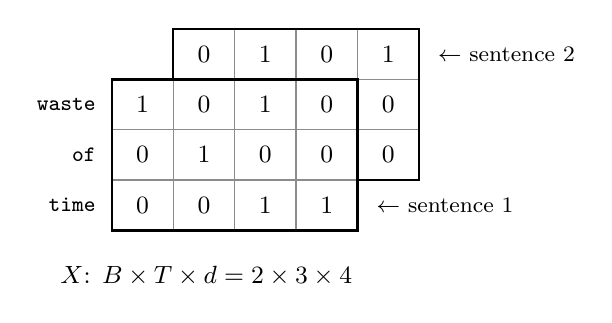
\begin{tikzpicture}
\fill[white] (0.780,0.640) rectangle (3.900,-1.279);
\draw[black!45, fill=white] (0.780,0.640) rectangle (1.560,0.000);
\node[font=\small, text=black] at (1.170,0.320) {$0$};
\draw[black!45, fill=white] (1.560,0.640) rectangle (2.340,0.000);
\node[font=\small, text=black] at (1.950,0.320) {$1$};
\draw[black!45, fill=white] (2.340,0.640) rectangle (3.120,0.000);
\node[font=\small, text=black] at (2.730,0.320) {$0$};
\draw[black!45, fill=white] (3.120,0.640) rectangle (3.900,0.000);
\node[font=\small, text=black] at (3.510,0.320) {$1$};
\draw[black!45, fill=white] (0.780,0.000) rectangle (1.560,-0.640);
\node[font=\small, text=black] at (1.170,-0.320) {$1$};
\draw[black!45, fill=white] (1.560,0.000) rectangle (2.340,-0.640);
\node[font=\small, text=black] at (1.950,-0.320) {$0$};
\draw[black!45, fill=white] (2.340,0.000) rectangle (3.120,-0.640);
\node[font=\small, text=black] at (2.730,-0.320) {$0$};
\draw[black!45, fill=white] (3.120,0.000) rectangle (3.900,-0.640);
\node[font=\small, text=black] at (3.510,-0.320) {$0$};
\draw[black!45, fill=white] (0.780,-0.640) rectangle (1.560,-1.279);
\node[font=\small, text=black] at (1.170,-0.959) {$0$};
\draw[black!45, fill=white] (1.560,-0.640) rectangle (2.340,-1.279);
\node[font=\small, text=black] at (1.950,-0.959) {$0$};
\draw[black!45, fill=white] (2.340,-0.640) rectangle (3.120,-1.279);
\node[font=\small, text=black] at (2.730,-0.959) {$1$};
\draw[black!45, fill=white] (3.120,-0.640) rectangle (3.900,-1.279);
\node[font=\small, text=black] at (3.510,-0.959) {$0$};
\draw[line width=0.9pt] (0.780,0.640) rectangle (3.900,-1.279);
\node[anchor=west, font=\footnotesize] at (4.020,0.320) {$\leftarrow$ sentence 2};
\fill[white] (0.000,0.000) rectangle (3.120,-1.919);
\draw[black!45, fill=white] (0.000,0.000) rectangle (0.780,-0.640);
\node[font=\small, text=black] at (0.390,-0.320) {$1$};
\draw[black!45, fill=white] (0.780,0.000) rectangle (1.560,-0.640);
\node[font=\small, text=black] at (1.170,-0.320) {$0$};
\draw[black!45, fill=white] (1.560,0.000) rectangle (2.340,-0.640);
\node[font=\small, text=black] at (1.950,-0.320) {$1$};
\draw[black!45, fill=white] (2.340,0.000) rectangle (3.120,-0.640);
\node[font=\small, text=black] at (2.730,-0.320) {$0$};
\draw[black!45, fill=white] (0.000,-0.640) rectangle (0.780,-1.279);
\node[font=\small, text=black] at (0.390,-0.959) {$0$};
\draw[black!45, fill=white] (0.780,-0.640) rectangle (1.560,-1.279);
\node[font=\small, text=black] at (1.170,-0.959) {$1$};
\draw[black!45, fill=white] (1.560,-0.640) rectangle (2.340,-1.279);
\node[font=\small, text=black] at (1.950,-0.959) {$0$};
\draw[black!45, fill=white] (2.340,-0.640) rectangle (3.120,-1.279);
\node[font=\small, text=black] at (2.730,-0.959) {$0$};
\draw[black!45, fill=white] (0.000,-1.279) rectangle (0.780,-1.919);
\node[font=\small, text=black] at (0.390,-1.599) {$0$};
\draw[black!45, fill=white] (0.780,-1.279) rectangle (1.560,-1.919);
\node[font=\small, text=black] at (1.170,-1.599) {$0$};
\draw[black!45, fill=white] (1.560,-1.279) rectangle (2.340,-1.919);
\node[font=\small, text=black] at (1.950,-1.599) {$1$};
\draw[black!45, fill=white] (2.340,-1.279) rectangle (3.120,-1.919);
\node[font=\small, text=black] at (2.730,-1.599) {$1$};
\draw[line width=0.9pt] (0.000,0.000) rectangle (3.120,-1.919);
\node[anchor=east, font=\footnotesize\ttfamily] at (-0.080,-0.320) {waste};
\node[anchor=east, font=\footnotesize\ttfamily] at (-0.080,-0.959) {of};
\node[anchor=east, font=\footnotesize\ttfamily] at (-0.080,-1.599) {time};
\node[anchor=west, font=\footnotesize] at (3.240,-1.599) {$\leftarrow$ sentence 1};
\node[anchor=north, font=\small] at (1.2,-2.25) {$X$: $B\times T\times d = 2\times3\times4$};
\end{tikzpicture}
\qquad
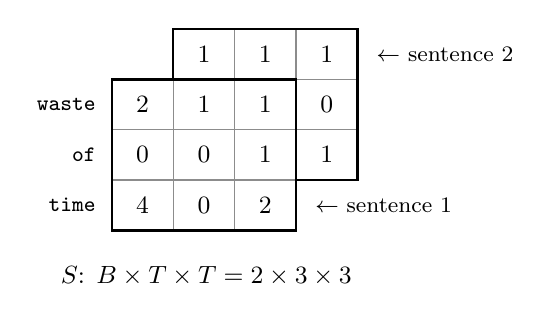
\begin{tikzpicture}
\fill[white] (0.780,0.640) rectangle (3.120,-1.279);
\draw[black!45, fill=white] (0.780,0.640) rectangle (1.560,0.000);
\node[font=\small, text=black] at (1.170,0.320) {$1$};
\draw[black!45, fill=white] (1.560,0.640) rectangle (2.340,0.000);
\node[font=\small, text=black] at (1.950,0.320) {$1$};
\draw[black!45, fill=white] (2.340,0.640) rectangle (3.120,0.000);
\node[font=\small, text=black] at (2.730,0.320) {$1$};
\draw[black!45, fill=white] (0.780,0.000) rectangle (1.560,-0.640);
\node[font=\small, text=black] at (1.170,-0.320) {$1$};
\draw[black!45, fill=white] (1.560,0.000) rectangle (2.340,-0.640);
\node[font=\small, text=black] at (1.950,-0.320) {$0$};
\draw[black!45, fill=white] (2.340,0.000) rectangle (3.120,-0.640);
\node[font=\small, text=black] at (2.730,-0.320) {$0$};
\draw[black!45, fill=white] (0.780,-0.640) rectangle (1.560,-1.279);
\node[font=\small, text=black] at (1.170,-0.959) {$0$};
\draw[black!45, fill=white] (1.560,-0.640) rectangle (2.340,-1.279);
\node[font=\small, text=black] at (1.950,-0.959) {$1$};
\draw[black!45, fill=white] (2.340,-0.640) rectangle (3.120,-1.279);
\node[font=\small, text=black] at (2.730,-0.959) {$1$};
\draw[line width=0.9pt] (0.780,0.640) rectangle (3.120,-1.279);
\node[anchor=west, font=\footnotesize] at (3.240,0.320) {$\leftarrow$ sentence 2};
\fill[white] (0.000,0.000) rectangle (2.340,-1.919);
\draw[black!45, fill=white] (0.000,0.000) rectangle (0.780,-0.640);
\node[font=\small, text=black] at (0.390,-0.320) {$2$};
\draw[black!45, fill=white] (0.780,0.000) rectangle (1.560,-0.640);
\node[font=\small, text=black] at (1.170,-0.320) {$1$};
\draw[black!45, fill=white] (1.560,0.000) rectangle (2.340,-0.640);
\node[font=\small, text=black] at (1.950,-0.320) {$1$};
\draw[black!45, fill=white] (0.000,-0.640) rectangle (0.780,-1.279);
\node[font=\small, text=black] at (0.390,-0.959) {$0$};
\draw[black!45, fill=white] (0.780,-0.640) rectangle (1.560,-1.279);
\node[font=\small, text=black] at (1.170,-0.959) {$0$};
\draw[black!45, fill=white] (1.560,-0.640) rectangle (2.340,-1.279);
\node[font=\small, text=black] at (1.950,-0.959) {$1$};
\draw[black!45, fill=white] (0.000,-1.279) rectangle (0.780,-1.919);
\node[font=\small, text=black] at (0.390,-1.599) {$4$};
\draw[black!45, fill=white] (0.780,-1.279) rectangle (1.560,-1.919);
\node[font=\small, text=black] at (1.170,-1.599) {$0$};
\draw[black!45, fill=white] (1.560,-1.279) rectangle (2.340,-1.919);
\node[font=\small, text=black] at (1.950,-1.599) {$2$};
\draw[line width=0.9pt] (0.000,0.000) rectangle (2.340,-1.919);
\node[anchor=east, font=\footnotesize\ttfamily] at (-0.080,-0.320) {waste};
\node[anchor=east, font=\footnotesize\ttfamily] at (-0.080,-0.959) {of};
\node[anchor=east, font=\footnotesize\ttfamily] at (-0.080,-1.599) {time};
\node[anchor=west, font=\footnotesize] at (2.460,-1.599) {$\leftarrow$ sentence 1};
\node[anchor=north, font=\small] at (1.2,-2.25) {$S$: $B\times T\times T = 2\times3\times3$};
\end{tikzpicture}
\\[14pt]
% AUTO-GENERATED by code/figlib.py helpers -- do not edit
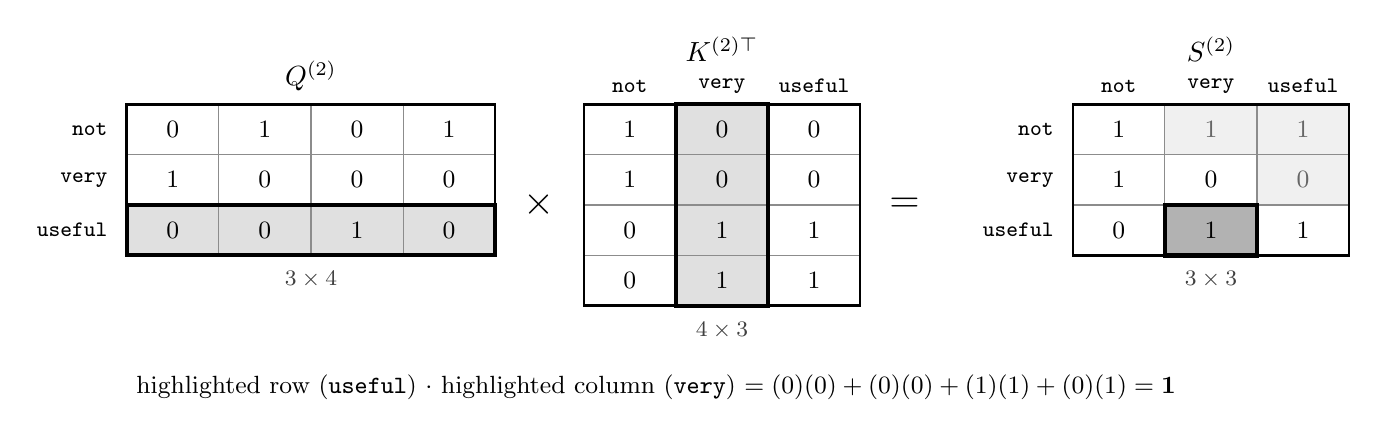
\begin{tikzpicture}[x=1.5cm]
\draw[black!45, fill=white] (0.000,0.000) rectangle (0.780,-0.640);
\node[font=\small, text=black] at (0.390,-0.320) {$0$};
\draw[black!45, fill=white] (0.780,0.000) rectangle (1.560,-0.640);
\node[font=\small, text=black] at (1.170,-0.320) {$1$};
\draw[black!45, fill=white] (1.560,0.000) rectangle (2.340,-0.640);
\node[font=\small, text=black] at (1.950,-0.320) {$0$};
\draw[black!45, fill=white] (2.340,0.000) rectangle (3.120,-0.640);
\node[font=\small, text=black] at (2.730,-0.320) {$1$};
\draw[black!45, fill=white] (0.000,-0.640) rectangle (0.780,-1.279);
\node[font=\small, text=black] at (0.390,-0.959) {$1$};
\draw[black!45, fill=white] (0.780,-0.640) rectangle (1.560,-1.279);
\node[font=\small, text=black] at (1.170,-0.959) {$0$};
\draw[black!45, fill=white] (1.560,-0.640) rectangle (2.340,-1.279);
\node[font=\small, text=black] at (1.950,-0.959) {$0$};
\draw[black!45, fill=white] (2.340,-0.640) rectangle (3.120,-1.279);
\node[font=\small, text=black] at (2.730,-0.959) {$0$};
\draw[black!45, fill=black!12] (0.000,-1.279) rectangle (0.780,-1.919);
\node[font=\small, text=black] at (0.390,-1.599) {$0$};
\draw[black!45, fill=black!12] (0.780,-1.279) rectangle (1.560,-1.919);
\node[font=\small, text=black] at (1.170,-1.599) {$0$};
\draw[black!45, fill=black!12] (1.560,-1.279) rectangle (2.340,-1.919);
\node[font=\small, text=black] at (1.950,-1.599) {$1$};
\draw[black!45, fill=black!12] (2.340,-1.279) rectangle (3.120,-1.919);
\node[font=\small, text=black] at (2.730,-1.599) {$0$};
\draw[line width=1.4pt] (0.000,-1.279) rectangle (3.120,-1.919);
\draw[line width=0.9pt] (0.000,0.000) rectangle (3.120,-1.919);
\node[anchor=east, font=\footnotesize\ttfamily] at (-0.080,-0.320) {not};
\node[anchor=east, font=\footnotesize\ttfamily] at (-0.080,-0.959) {very};
\node[anchor=east, font=\footnotesize\ttfamily] at (-0.080,-1.599) {useful};
\node[anchor=south, font=\normalsize] at (1.560,0.050) {$Q^{(2)}$};
\node[anchor=north, font=\footnotesize, text=black!75] at (1.560,-1.999) {$3\times4$};
\draw[black!45, fill=white] (3.870,0.000) rectangle (4.650,-0.640);
\node[font=\small, text=black] at (4.260,-0.320) {$1$};
\draw[black!45, fill=black!12] (4.650,0.000) rectangle (5.430,-0.640);
\node[font=\small, text=black] at (5.040,-0.320) {$0$};
\draw[black!45, fill=white] (5.430,0.000) rectangle (6.210,-0.640);
\node[font=\small, text=black] at (5.820,-0.320) {$0$};
\draw[black!45, fill=white] (3.870,-0.640) rectangle (4.650,-1.279);
\node[font=\small, text=black] at (4.260,-0.959) {$1$};
\draw[black!45, fill=black!12] (4.650,-0.640) rectangle (5.430,-1.279);
\node[font=\small, text=black] at (5.040,-0.959) {$0$};
\draw[black!45, fill=white] (5.430,-0.640) rectangle (6.210,-1.279);
\node[font=\small, text=black] at (5.820,-0.959) {$0$};
\draw[black!45, fill=white] (3.870,-1.279) rectangle (4.650,-1.919);
\node[font=\small, text=black] at (4.260,-1.599) {$0$};
\draw[black!45, fill=black!12] (4.650,-1.279) rectangle (5.430,-1.919);
\node[font=\small, text=black] at (5.040,-1.599) {$1$};
\draw[black!45, fill=white] (5.430,-1.279) rectangle (6.210,-1.919);
\node[font=\small, text=black] at (5.820,-1.599) {$1$};
\draw[black!45, fill=white] (3.870,-1.919) rectangle (4.650,-2.558);
\node[font=\small, text=black] at (4.260,-2.239) {$0$};
\draw[black!45, fill=black!12] (4.650,-1.919) rectangle (5.430,-2.558);
\node[font=\small, text=black] at (5.040,-2.239) {$1$};
\draw[black!45, fill=white] (5.430,-1.919) rectangle (6.210,-2.558);
\node[font=\small, text=black] at (5.820,-2.239) {$1$};
\draw[line width=1.4pt] (4.650,0.000) rectangle (5.430,-2.558);
\draw[line width=0.9pt] (3.870,0.000) rectangle (6.210,-2.558);
\node[anchor=south, font=\footnotesize\ttfamily] at (4.260,0.020) {not};
\node[anchor=south, font=\footnotesize\ttfamily] at (5.040,0.020) {very};
\node[anchor=south, font=\footnotesize\ttfamily] at (5.820,0.020) {useful};
\node[anchor=south, font=\normalsize] at (5.040,0.420) {$K^{(2)\top}$};
\node[anchor=north, font=\footnotesize, text=black!75] at (5.040,-2.638) {$4\times3$};
\draw[black!45, fill=white] (8.010,0.000) rectangle (8.790,-0.640);
\node[font=\small, text=black] at (8.400,-0.320) {$1$};
\draw[black!45, fill=black!6] (8.790,0.000) rectangle (9.570,-0.640);
\node[font=\small, text=black!60] at (9.180,-0.320) {$1$};
\draw[black!45, fill=black!6] (9.570,0.000) rectangle (10.350,-0.640);
\node[font=\small, text=black!60] at (9.960,-0.320) {$1$};
\draw[black!45, fill=white] (8.010,-0.640) rectangle (8.790,-1.279);
\node[font=\small, text=black] at (8.400,-0.959) {$1$};
\draw[black!45, fill=white] (8.790,-0.640) rectangle (9.570,-1.279);
\node[font=\small, text=black] at (9.180,-0.959) {$0$};
\draw[black!45, fill=black!6] (9.570,-0.640) rectangle (10.350,-1.279);
\node[font=\small, text=black!60] at (9.960,-0.959) {$0$};
\draw[black!45, fill=white] (8.010,-1.279) rectangle (8.790,-1.919);
\node[font=\small, text=black] at (8.400,-1.599) {$0$};
\draw[black!45, fill=black!30] (8.790,-1.279) rectangle (9.570,-1.919);
\node[font=\small, text=black] at (9.180,-1.599) {$1$};
\draw[black!45, fill=white] (9.570,-1.279) rectangle (10.350,-1.919);
\node[font=\small, text=black] at (9.960,-1.599) {$1$};
\draw[line width=1.6pt] (8.790,-1.279) rectangle (9.570,-1.919);
\draw[line width=0.9pt] (8.010,0.000) rectangle (10.350,-1.919);
\node[anchor=east, font=\footnotesize\ttfamily] at (7.930,-0.320) {not};
\node[anchor=east, font=\footnotesize\ttfamily] at (7.930,-0.959) {very};
\node[anchor=east, font=\footnotesize\ttfamily] at (7.930,-1.599) {useful};
\node[anchor=south, font=\footnotesize\ttfamily] at (8.400,0.020) {not};
\node[anchor=south, font=\footnotesize\ttfamily] at (9.180,0.020) {very};
\node[anchor=south, font=\footnotesize\ttfamily] at (9.960,0.020) {useful};
\node[anchor=south, font=\normalsize] at (9.180,0.420) {$S^{(2)}$};
\node[anchor=north, font=\footnotesize, text=black!75] at (9.180,-1.999) {$3\times3$};
\node[font=\Large] at (3.495,-1.279) {$\times$};
\node[font=\Large] at (6.585,-1.279) {$=$};
\node[anchor=north west, font=\small, align=left] at (0,-3.308) {highlighted row (\texttt{useful}) $\cdot$ highlighted column (\texttt{very}) $= (0)(0) + (0)(0) + (1)(1) + (0)(1) = \mathbf{1}$};
\end{tikzpicture}
\\[10pt]
% AUTO-GENERATED by code/figlib.py helpers -- do not edit
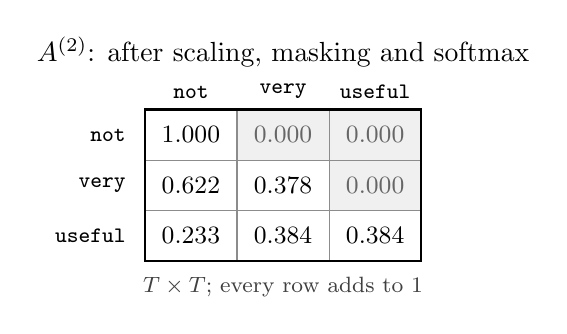
\begin{tikzpicture}[x=1.5cm]
\draw[black!45, fill=white] (0.000,0.000) rectangle (0.780,-0.640);
\node[font=\small, text=black] at (0.390,-0.320) {$1.000$};
\draw[black!45, fill=black!6] (0.780,0.000) rectangle (1.560,-0.640);
\node[font=\small, text=black!60] at (1.170,-0.320) {$0.000$};
\draw[black!45, fill=black!6] (1.560,0.000) rectangle (2.340,-0.640);
\node[font=\small, text=black!60] at (1.950,-0.320) {$0.000$};
\draw[black!45, fill=white] (0.000,-0.640) rectangle (0.780,-1.279);
\node[font=\small, text=black] at (0.390,-0.959) {$0.622$};
\draw[black!45, fill=white] (0.780,-0.640) rectangle (1.560,-1.279);
\node[font=\small, text=black] at (1.170,-0.959) {$0.378$};
\draw[black!45, fill=black!6] (1.560,-0.640) rectangle (2.340,-1.279);
\node[font=\small, text=black!60] at (1.950,-0.959) {$0.000$};
\draw[black!45, fill=white] (0.000,-1.279) rectangle (0.780,-1.919);
\node[font=\small, text=black] at (0.390,-1.599) {$0.233$};
\draw[black!45, fill=white] (0.780,-1.279) rectangle (1.560,-1.919);
\node[font=\small, text=black] at (1.170,-1.599) {$0.384$};
\draw[black!45, fill=white] (1.560,-1.279) rectangle (2.340,-1.919);
\node[font=\small, text=black] at (1.950,-1.599) {$0.384$};
\draw[line width=0.9pt] (0.000,0.000) rectangle (2.340,-1.919);
\node[anchor=east, font=\footnotesize\ttfamily] at (-0.080,-0.320) {not};
\node[anchor=east, font=\footnotesize\ttfamily] at (-0.080,-0.959) {very};
\node[anchor=east, font=\footnotesize\ttfamily] at (-0.080,-1.599) {useful};
\node[anchor=south, font=\footnotesize\ttfamily] at (0.390,0.020) {not};
\node[anchor=south, font=\footnotesize\ttfamily] at (1.170,0.020) {very};
\node[anchor=south, font=\footnotesize\ttfamily] at (1.950,0.020) {useful};
\node[anchor=south, font=\normalsize] at (1.170,0.420) {$A^{(2)}$: after scaling, masking and softmax};
\node[anchor=north, font=\footnotesize, text=black!75] at (1.170,-1.999) {$T\times T$; every row adds to 1};
\end{tikzpicture}

\caption{Top: a batch of $B=2$ sentences. Each sentence keeps its own $3\times4$ matrix $X$ and gets its own
$3\times3$ table $S$. Bottom: the second sentence's table, built by the same multiplication as in
Figure~\ref{fig:qkv}'s machines, and its shares after scaling, masking and softmax.}
\end{figure}

\Picture Two classrooms run the same handshake tournament in parallel, each with its own table. Nobody shakes hands with
the other classroom.

\begin{breaks}
Two real classrooms would need two organisers. Here one multiplication fills both tables; they are separate only
because the numbers are arranged that way.
\end{breaks}

\Exactly Stack the sentences into one block of numbers of shape $B\times T\times d = 2\times3\times4$. The same
machines $W_Q, W_K, W_V$ apply to every token of every sentence, so $Q, K, V$ have shape $B\times T\times d_k$. The
transpose now flips only the last two axes of $K$, and
\[
S = QK^\top \shape{(B\times T\times d_k)(B\times d_k\times T) = B\times T\times T}
\]
is $B$ tournament tables computed side by side: \nScores\ scores in one operation, with no score ever mixing the two
sentences. After the mask and softmax, $O=AV$ has shape $B\times T\times d_k$, and every one of its $B\times T =
\nPreds$ rows will go on to make a next-word guess. Our script checks that sentence 1 gives exactly the same numbers
in the batch as it gave alone.

\Why This is where Chapter 1's history pays off. The RNN had to walk each sentence word by word. Here a batch of $B$
sentences of $T$ tokens is a handful of large matrix multiplications, and those multiplications are what GPUs are
made of.

\Summary{A batch is $B$ separate attention tables computed in one operation, giving $B\times T$ guesses per pass.}

%---------------------------------------------------------------------
\subsection*{3.10\quad How learning shapes the arrows}

Our toy machines were chosen by hand. In a real model, $W_Q$, $W_K$ and $W_V$ start as random numbers and are learned
from the next-word game. Chapter 8 does the bookkeeping; here is the whole idea as a picture.

Every score is $\lVert\bm{q}\rVert\lVert\bm{k}\rVert\cos\theta$, so there are only two ways to change how much one
token attends to another: \emph{turn} the arrows (change the angle) or \emph{stretch} them (change the length).
Training plays the game millions of times. Each time the model guesses the next word, it checks the answer, and
every weight is nudged a tiny step in the direction that would have made the right word a little more likely:
\begin{itemize}
\item if looking more at \tok{waste} would have helped \tok{time} predict \tok{Sorry}, the query of \tok{time} is
turned a little towards the key of \tok{waste} (and that key a little towards the query);
\item if looking at \tok{of} only added noise, the arrows are turned a little apart;
\item if the right choice was clear, the query is stretched, making the softmax more decisive (\S3.7);
\item and the value arrows are turned towards whatever turned out to be useful to hand over.
\end{itemize}

\begin{figure}[h]
\centering
\begin{tikzpicture}[scale=1.25, font=\footnotesize]
\draw[-{Stealth}, thick] (0,0) -- (3.2,0) node[right] {key of \tok{waste}};
\draw[-{Stealth}, thick, black!65] (0,0) -- (-1.2,1.3) node[left, text=black] {key of \tok{of}};
\draw[-{Stealth}, thick, dashed, black!65] (0,0) -- (0.4,1.5) node[above, text=black] {query of \tok{time}, at the start};
\draw[-{Stealth}, very thick] (0,0) -- (2.7,1.2) node[right] {query after training};
\draw[-{Stealth}, black!60] (0.31,1.16) arc[start angle=75, end angle=30, radius=1.2];
\end{tikzpicture}
\caption{Learning as turning and stretching arrows (schematic, not to scale). The query is turned towards the key
that helped, away from the one that did not, and stretched to be more confident. Training never moves the arrows
directly; it changes the machines $W_Q, W_K, W_V$ that produce them.}
\end{figure}

\begin{breaks}
The figure turns one arrow. Training turns the \emph{machines}, so every arrow those machines produce turns
together, including arrows for sentences that are not in this batch.
\end{breaks}

That last point makes this powerful. A nudge learned from \tok{waste of time} also moves the arrows produced for
\tok{waste of money} and \tok{waste of effort}, because those words have nearby arrows (Requirement 1). That is how
a model trained on finitely many sentences handles sentences it has never seen, the exact thing the counting
notebook of \S1.3 could not do.

\Summary{Learning only turns and stretches arrows, by adjusting the machines that make them, so lessons spread to
similar words.}

%---------------------------------------------------------------------
\subsection*{3.11\quad What we built, and the next failure}

\begin{principle}{attention is a soft lookup table}
A Python dictionary takes a query, finds the one key that matches \emph{exactly}, and returns its value. Attention
does the same, softly: every key matches a little, measured by a dot product, and you get a blend of all the values.
Because ``a little'' is a smooth number, the lookup can be learned. The same pattern appears whenever a system must
pick from candidates by relevance: a search engine ranking documents, a recommender ranking products, or the
retriever in an AI agent's memory system, which scores stored memories against the current conversation and decides
how much of each one reaches the model.
\end{principle}

\Predict Swap the first two tokens and feed \tok{of waste time}. Will the output for \tok{time} change?

The output for \tok{time} is
\[ \bm{o}_{\text{time}} = \oTimeSwap, \]
\emph{identical} to before. The mask decides who may look at whom, but the scores themselves cannot tell \tok{waste
of} from \tok{of waste}: to \tok{time}, its past is a bag, not a sequence. We have quietly lost Requirement 2, the
very thing the RNN gave us for free, and we are back to the bag of words of \S1.4. Chapter 4 fixes it, and the fix
(RoPE) turns out to be a \emph{rotation} of exactly these query and key arrows, by an angle that depends on the
position.

\begin{wrongidea}{3.10}
\emph{Attention already knows the order of the words.} Masking is about order, so it seems order must be handled. But none of $W_Q$, $W_K$, $W_V$
sees a position. The mask only says which tokens are visible; among the visible ones, attention cannot tell who
came first.
\end{wrongidea}

\begin{checkq}
Feed \tok{of waste time} instead of \tok{waste of time}. What happens to the output for \tok{time}?
\begin{options}
\item It is unchanged: \tok{time} sees the same set of earlier tokens, and nothing in the scores knows their order.
\item It changes, because the causal mask encodes word order.
\item It changes, because \tok{waste}'s value is now in a different row.
\item It changes, because the scores are percentages of position.
\end{options}
\end{checkq}

\Summary{Attention is a learnable soft lookup that meets Requirements 3 and 4, but on its own it cannot tell word
order.}

%---------------------------------------------------------------------
\begin{lookingback}
(1) Chapter 1: why does one sentence of $T$ tokens give $T$ training exercises? (2) Chapter 1: which requirement did
the RNN fail that attention now meets, and which one did attention lose? (3) Chapter 2: where do the rows of $X$ come
from? (4) Chapter 2: why does a tokenizer split a rare word into pieces instead of giving it its own token?
\end{lookingback}

\subsection*{Exercises}

\begin{exercise}
Compute by hand the attention output for the token \tok{of}. Then explain, using only the geometry of
$\bm{q}_{\text{of}}$ and the keys, why its two shares are equal.
\end{exercise}

\begin{exercise}
A model has $d_k=256$. Without scaling, roughly how far apart would the scores of unrelated tokens typically be? What
would you divide by, and why that number?
\end{exercise}

\begin{exercise}
Fill the gaps for the token \tok{useful} in the second sentence of \S3.9. Its raw scores are $(0, 1, 1)$. After
dividing by $\sqrt{d_k}$ they are $(\rule{1em}{0.4pt}, \rule{1em}{0.4pt}, \rule{1em}{0.4pt})$. Exponentiate, divide by the
total, and check your answer against the last row of $A^{(2)}$.
\end{exercise}

\begin{exercise}
A second customer has clues $\nThreeClTwo$ with the same importances $\nThreeW$. Compute the churn score. Is the
customer arrow pointing with or against the importance arrow?
\end{exercise}

\subsection*{Answers to Chapter 3}
\small
\textbf{Check yourself 3.1.} (b). (a) is M3.1: the arrow does not change with context. (c) is the uniform average
that \S3.1 showed cannot learn. (d) is a real issue (Chapter 4), but even with positions, one arrow cannot see its
neighbours.

\textbf{Check yourself 3.2.} (b). (a) is M3.8: $\bm{b}$ wins on dot product only because it is longer. (c) mixes up
``positive'' with ``equal''. (d): the angles answer it without drawing.

\textbf{Check yourself 3.3.} (a). (b) and (c) are M3.9: the transpose changes no arrow. (d) is wrong because $QK$ is
not defined.

\textbf{Check yourself 3.4.} (b). (a) is M3.4, (c) is M3.6, (d) is M3.5.

\textbf{Check yourself 3.5.} (b). (a) is M3.7: the mask is also what lets all rows train together. (c) is M3.2.
(d) is false: \tok{time} gives \apctTime\% to itself.

\textbf{Check yourself 3.6.} (a), for reason (i). Softmax gives $(\nThreeSoft)$ for both lists. (b) is M3.2. (c) is
M3.11: dividing by the total would give $(\nThreeRatioB)$, the shift option (c) expects. (d) is M3.8.

\textbf{Check yourself 3.7.} (b). (a) is M3.3. (c) is M3.2: softmax does that. (d) is true in the toy only.

\textbf{Check yourself 3.8.} (a). (b) is M3.10. (c): the rows moved, but the set of value arrows \tok{time} blends is
the same. (d) mixes two wrong ideas.

\textbf{Looking back.} (1) Each prefix asks for its own next word, and the mask lets all prefixes be answered in one
pass. (2) Attention meets Requirement 3 (direct reach) and loses Requirement 2 (order). (3) Each token id picks one
row of the embedding table. (4) So the vocabulary stays a fixed size and no word is ever unknown: a rare word becomes
known pieces.

\textbf{Exercise 3.1.} $\bm{q}_{\text{of}}=(0,1,0,0)$ points along the second direction only. Both
$\bm{k}_{\text{waste}}$ and $\bm{k}_{\text{of}}$ have 0 there: both are at right angles to the query, so both scores
are 0, the softmax of $(0,0)$ is $(0.5,0.5)$, and $\bm{o}_{\text{of}} = 0.5\,\bm{v}_{\text{waste}}+0.5\,\bm{v}_{\text{of}}
= \oOf$. A query at right angles to every key has nothing to prefer, and attention falls back to the plain average of
\S3.1. \emph{Uniform attention is what ``no information'' looks like.}

\textbf{Exercise 3.2.} About $\sqrt{256}=\nThreeRootTwoFiftySix$ points, enough for softmax to put nearly all its
weight on one key at random. Divide by $\sqrt{256}$ to bring the typical spread back to about one point, whatever
$d_k$ is.

\textbf{Exercise 3.3.} $(0, 0.5, 0.5)$; the two equal scores give equal shares, and the last row of $A^{(2)}$ shows the
result. The strategy that works: do one row at a time, and check the shares add to 1.

\textbf{Exercise 3.4.} $\nThreeClTwo\cdot\nThreeW = \nThreeScoreTwo$. Negative: the customer arrow points partly
against the importance arrow.
\normalsize

\subsection*{What you now know}
\begin{itemize}
\item The dot product as weighted clues, as a shadow, and as lengths times agreement, and why the two formulas match.
\item A matrix as recipe cards and as a machine that moves arrows; the transpose as standing keys up as columns.
\item Queries, keys and values, and a full attention computation by hand, with masking and softmax.
\item Why softmax uses $e^x$, why scores are divided by $\sqrt{d_k}$, and how a batch runs in one operation.
\item Learning as turning and stretching arrows, and the next failure: attention alone ignores order.
\end{itemize}

\clearpage\newpage
\section*{4\quad Order: from sinusoids to rotations (RoPE)}
\addcontentsline{toc}{section}{4 Order: from sinusoids to rotations}
\startchapter{4}
\ifdefined\fitwidthFourFive\else
\newsavebox{\fitboxFourFive}
\newcommand{\fitwidthFourFive}[1]{\sbox{\fitboxFourFive}{\begin{tabular}{@{}c@{}}#1\end{tabular}}\ifdim\wd\fitboxFourFive>\linewidth\resizebox{\linewidth}{!}{\usebox{\fitboxFourFive}}\else\usebox{\fitboxFourFive}\fi}
\fi

\begin{chaptermap}
Chapter 3 ended with a failure: attention cannot tell \tok{waste of time} from \tok{of waste time}. This
chapter gives the model a sense of order. We follow the fixes in the order researchers found them:
learning a vector for each position (GPT-2), adding fixed waves (the 2017 transformer), and finally
rotating the queries and keys by an angle that grows with position (RoPE, used by Qwen3 and most current
models). On the way we prove, with numbers, the property that makes rotation the winner: the score
between two tokens depends only on \emph{how far apart} they are.
\end{chaptermap}

\machine{4}{You are here: Chapter 4 adds the \emph{positions} box on the left. It does not add a new
layer to the stack. It turns each query and key inside attention by an angle that depends on where the
token stands, so attention can finally tell \tok{waste of time} from \tok{of waste time}.}

\begin{beforeyoustart}
(1) A clock's minute hand turns $6^\circ$ per minute. Where is it after 15 minutes?
(2) What are $\cos 0^\circ$, $\cos 90^\circ$ and $\cos 180^\circ$? (3) If you turn an arrow without
stretching it, does its length change? (4) The second hand of a clock and the hour hand both point at
12. Can you tell the time from the second hand alone?

\smallskip\noindent\textit{Refreshers.} (1) $15\times6^\circ = 90^\circ$: pointing at 3. (2) 1, 0 and
$-1$: same direction, right angle, opposite. (3) No; turning keeps the length. (4) No: it repeats every
minute, so you also need the slower hands. Keep this last answer in mind; it is the whole idea of
\S4.6.
\end{beforeyoustart}

%---------------------------------------------------------------------
\subsection*{4.1\quad The failure, once more}

\Predict In Chapter 3 we fed \tok{of waste time} instead of \tok{waste of time}. Before looking back,
guess: did the output for \tok{time} change a lot, a little, or not at all?

Not at all. Both orders give $\bm{o}_{\text{time}} = \nFourNoPosTime$. Look at where order could have entered
the computation. The queries, keys and values are made from each token's own arrow, and the token's
arrow is the same wherever it stands. The score $\bm{q}\cdot\bm{k}$ only sees the two arrows. The mask only
decides which tokens are visible. So to \tok{time}, its past is a bag, as in the bag-of-words attempt of
\S1.4. For a support reply this is serious: \tok{not useful, very good} and \tok{very useful, not good}
would look alike once again.

\begin{wrongidea}{4.1}
``The mask already tells the model the order.'' The mask tells each token \emph{which} tokens it may
see. It says nothing about \emph{where} they stand. It is tempting because the mask is drawn as a triangle
in reading order, so order seems to be built in. But none of $W_Q$, $W_K$, $W_V$ sees a position, and \S4.1
shows it with numbers: same set of earlier tokens, same output.
\end{wrongidea}

\Summary{attention compares arrows that carry no position, so we have to put position into the arrows
ourselves.}

%---------------------------------------------------------------------
\subsection*{4.2\quad Attempt: add a position vector}

\Predict The simplest idea: add the position number to the arrow, so the first token gets $+0$, the
second $+1$, and so on. Can you see a problem with token number 1000?

\Picture Give every seat in a cinema a small badge with its seat number, and pin it onto whoever sits
there. The person is the same; the badge says where they are.

\paragraph{Why plain numbers fail.} If you add $1000$ to every coordinate of the 1000th token, its arrow
is dominated by the badge and the word is lost: $(0,0,1,1)$ becomes $(1000,1000,1001,1001)$, and every
token far into a long text looks the same. The badge has to stay small, and it has to look different at
every position.

\paragraph{Two ways to make good badges.} GPT-2 (Radford and colleagues, 2019) \emph{learned} a table of
badges, one row per position, exactly like the embedding table of Chapter 2: 1024 positions, so it
cannot handle a 1025th token at all. The original transformer (Vaswani and colleagues, 2017) used
\emph{fixed waves} instead. For position $p$ and coordinate pair $i$ (pairs $0,1$; $2,3$; \ldots),
\[
\mathrm{PE}(p, 2i) = \sin\!\Big(\frac{p}{10000^{2i/d}}\Big), \qquad
\mathrm{PE}(p, 2i+1) = \cos\!\Big(\frac{p}{10000^{2i/d}}\Big).
\]
Each pair of coordinates is a wave with its own speed. For our toy, $d=4$ and positions $0,1,2$, so
the badges form a $T\times d = 3\times4$ table, one row per position. Figure~\ref{fig:ch4pe} adds it to
the token arrows, cell by cell.

\begin{center}
\fitwidthFourFive{% AUTO-GENERATED by code/figlib.py helpers -- do not edit
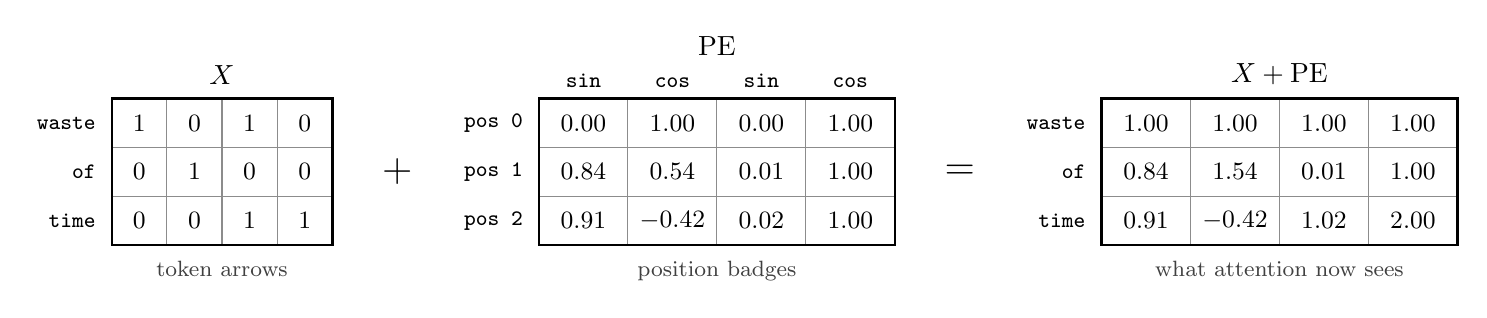
\begin{tikzpicture}
\draw[black!45, fill=white] (0.975,0.930) rectangle (1.675,0.310);
\node[font=\small, text=black] at (1.325,0.620) {$1$};
\draw[black!45, fill=white] (1.675,0.930) rectangle (2.375,0.310);
\node[font=\small, text=black] at (2.025,0.620) {$0$};
\draw[black!45, fill=white] (2.375,0.930) rectangle (3.075,0.310);
\node[font=\small, text=black] at (2.725,0.620) {$1$};
\draw[black!45, fill=white] (3.075,0.930) rectangle (3.775,0.310);
\node[font=\small, text=black] at (3.425,0.620) {$0$};
\draw[black!45, fill=white] (0.975,0.310) rectangle (1.675,-0.310);
\node[font=\small, text=black] at (1.325,-0.000) {$0$};
\draw[black!45, fill=white] (1.675,0.310) rectangle (2.375,-0.310);
\node[font=\small, text=black] at (2.025,-0.000) {$1$};
\draw[black!45, fill=white] (2.375,0.310) rectangle (3.075,-0.310);
\node[font=\small, text=black] at (2.725,-0.000) {$0$};
\draw[black!45, fill=white] (3.075,0.310) rectangle (3.775,-0.310);
\node[font=\small, text=black] at (3.425,-0.000) {$0$};
\draw[black!45, fill=white] (0.975,-0.310) rectangle (1.675,-0.930);
\node[font=\small, text=black] at (1.325,-0.620) {$0$};
\draw[black!45, fill=white] (1.675,-0.310) rectangle (2.375,-0.930);
\node[font=\small, text=black] at (2.025,-0.620) {$0$};
\draw[black!45, fill=white] (2.375,-0.310) rectangle (3.075,-0.930);
\node[font=\small, text=black] at (2.725,-0.620) {$1$};
\draw[black!45, fill=white] (3.075,-0.310) rectangle (3.775,-0.930);
\node[font=\small, text=black] at (3.425,-0.620) {$1$};
\draw[line width=0.9pt] (0.975,0.930) rectangle (3.775,-0.930);
\node[anchor=east, font=\footnotesize\ttfamily] at (0.895,0.620) {waste};
\node[anchor=east, font=\footnotesize\ttfamily] at (0.895,-0.000) {of};
\node[anchor=east, font=\footnotesize\ttfamily] at (0.895,-0.620) {time};
\node[anchor=south, font=\normalsize] at (2.375,0.980) {$X$};
\node[anchor=north, font=\footnotesize, text=black!75] at (2.375,-1.010) {token arrows};
\node[font=\Large] at (4.600,0) {$+$};
\draw[black!45, fill=white] (6.400,0.930) rectangle (7.530,0.310);
\node[font=\small, text=black] at (6.965,0.620) {$0.00$};
\draw[black!45, fill=white] (7.530,0.930) rectangle (8.660,0.310);
\node[font=\small, text=black] at (8.095,0.620) {$1.00$};
\draw[black!45, fill=white] (8.660,0.930) rectangle (9.790,0.310);
\node[font=\small, text=black] at (9.225,0.620) {$0.00$};
\draw[black!45, fill=white] (9.790,0.930) rectangle (10.920,0.310);
\node[font=\small, text=black] at (10.355,0.620) {$1.00$};
\draw[black!45, fill=white] (6.400,0.310) rectangle (7.530,-0.310);
\node[font=\small, text=black] at (6.965,-0.000) {$0.84$};
\draw[black!45, fill=white] (7.530,0.310) rectangle (8.660,-0.310);
\node[font=\small, text=black] at (8.095,-0.000) {$0.54$};
\draw[black!45, fill=white] (8.660,0.310) rectangle (9.790,-0.310);
\node[font=\small, text=black] at (9.225,-0.000) {$0.01$};
\draw[black!45, fill=white] (9.790,0.310) rectangle (10.920,-0.310);
\node[font=\small, text=black] at (10.355,-0.000) {$1.00$};
\draw[black!45, fill=white] (6.400,-0.310) rectangle (7.530,-0.930);
\node[font=\small, text=black] at (6.965,-0.620) {$0.91$};
\draw[black!45, fill=white] (7.530,-0.310) rectangle (8.660,-0.930);
\node[font=\small, text=black] at (8.095,-0.620) {$-0.42$};
\draw[black!45, fill=white] (8.660,-0.310) rectangle (9.790,-0.930);
\node[font=\small, text=black] at (9.225,-0.620) {$0.02$};
\draw[black!45, fill=white] (9.790,-0.310) rectangle (10.920,-0.930);
\node[font=\small, text=black] at (10.355,-0.620) {$1.00$};
\draw[line width=0.9pt] (6.400,0.930) rectangle (10.920,-0.930);
\node[anchor=east, font=\footnotesize\ttfamily] at (6.320,0.620) {pos 0};
\node[anchor=east, font=\footnotesize\ttfamily] at (6.320,-0.000) {pos 1};
\node[anchor=east, font=\footnotesize\ttfamily] at (6.320,-0.620) {pos 2};
\node[anchor=south, font=\footnotesize\ttfamily] at (6.965,0.950) {sin};
\node[anchor=south, font=\footnotesize\ttfamily] at (8.095,0.950) {cos};
\node[anchor=south, font=\footnotesize\ttfamily] at (9.225,0.950) {sin};
\node[anchor=south, font=\footnotesize\ttfamily] at (10.355,0.950) {cos};
\node[anchor=south, font=\normalsize] at (8.660,1.350) {$\mathrm{PE}$};
\node[anchor=north, font=\footnotesize, text=black!75] at (8.660,-1.010) {position badges};
\node[font=\Large] at (11.745,0) {$=$};
\draw[black!45, fill=white] (13.545,0.930) rectangle (14.675,0.310);
\node[font=\small, text=black] at (14.110,0.620) {$1.00$};
\draw[black!45, fill=white] (14.675,0.930) rectangle (15.805,0.310);
\node[font=\small, text=black] at (15.240,0.620) {$1.00$};
\draw[black!45, fill=white] (15.805,0.930) rectangle (16.935,0.310);
\node[font=\small, text=black] at (16.370,0.620) {$1.00$};
\draw[black!45, fill=white] (16.935,0.930) rectangle (18.065,0.310);
\node[font=\small, text=black] at (17.500,0.620) {$1.00$};
\draw[black!45, fill=white] (13.545,0.310) rectangle (14.675,-0.310);
\node[font=\small, text=black] at (14.110,-0.000) {$0.84$};
\draw[black!45, fill=white] (14.675,0.310) rectangle (15.805,-0.310);
\node[font=\small, text=black] at (15.240,-0.000) {$1.54$};
\draw[black!45, fill=white] (15.805,0.310) rectangle (16.935,-0.310);
\node[font=\small, text=black] at (16.370,-0.000) {$0.01$};
\draw[black!45, fill=white] (16.935,0.310) rectangle (18.065,-0.310);
\node[font=\small, text=black] at (17.500,-0.000) {$1.00$};
\draw[black!45, fill=white] (13.545,-0.310) rectangle (14.675,-0.930);
\node[font=\small, text=black] at (14.110,-0.620) {$0.91$};
\draw[black!45, fill=white] (14.675,-0.310) rectangle (15.805,-0.930);
\node[font=\small, text=black] at (15.240,-0.620) {$-0.42$};
\draw[black!45, fill=white] (15.805,-0.310) rectangle (16.935,-0.930);
\node[font=\small, text=black] at (16.370,-0.620) {$1.02$};
\draw[black!45, fill=white] (16.935,-0.310) rectangle (18.065,-0.930);
\node[font=\small, text=black] at (17.500,-0.620) {$2.00$};
\draw[line width=0.9pt] (13.545,0.930) rectangle (18.065,-0.930);
\node[anchor=east, font=\footnotesize\ttfamily] at (13.465,0.620) {waste};
\node[anchor=east, font=\footnotesize\ttfamily] at (13.465,-0.000) {of};
\node[anchor=east, font=\footnotesize\ttfamily] at (13.465,-0.620) {time};
\node[anchor=south, font=\normalsize] at (15.805,0.980) {$X+\mathrm{PE}$};
\node[anchor=north, font=\footnotesize, text=black!75] at (15.805,-1.010) {what attention now sees};
\end{tikzpicture}
}
\captionof{figure}{Sinusoidal badges as a matrix. Row $p$ of $\mathrm{PE}$ is the badge for position $p$; it is
added to the token arrow in the same row. Notice the second pair of columns barely changes from row to
row (it is the slow wave), while the first pair changes a lot (the fast wave).}
\label{fig:ch4pe}
\end{center}

Every entry of $\mathrm{PE}$ stays between $-1$ and $1$, however long the text. Add these badges to the toy arrows and run
the attention of Chapter 3 again. \tok{time}'s output becomes $\nFourSinTime$ for \tok{waste of time} and
$\nFourSinTimeSwap$ for \tok{of waste time}. The two orders now differ (by up to \nFourSinDiff\ in one
coordinate). Requirement 2 is back.

\begin{figure}[h]
\centering
\begin{tikzpicture}
\begin{axis}[width=12cm, height=4.2cm, xlabel={position $p$}, ylabel={value},
  xlabel style={font=\small}, ylabel style={font=\small}, tick label style={font=\small},
  axis lines*=left, ymin=-1.15, ymax=1.15, xmin=0, xmax=40, legend style={font=\footnotesize, draw=none, at={(0.5,1.03)}, anchor=south}, legend columns=3]
\addplot[black, thick] table[x=pos, y=fast] {data_ch4/waves.dat};
\addplot[black!60, very thick, densely dotted] table[x=pos, y=mid] {data_ch4/waves.dat};
\addplot[black!70, thick, dashed] table[x=pos, y=slow] {data_ch4/waves.dat};
\legend{pair 0 (repeats every \nFourWlMin), pair 4 (every \nFourMidWl), pair 8 (every \nFourSlowWl)}
\end{axis}
\end{tikzpicture}
\caption{Three of the waves used for $d=64$: solid is fast, dotted is medium, dashed is slow. Fast waves tell neighbours apart; slow waves tell far
positions apart. For $d=64$ the repeat lengths run from \nFourWlMin\ to \nFourWlMax\ positions.}
\end{figure}

\begin{wrongidea}{4.2}
``Add the position number itself.'' The number grows without limit and swamps the word. A useful badge
has two properties at once: it stays small, and it is different at every position. Waves have both.
\end{wrongidea}

\begin{breaks}
A badge is pinned on and stays separate from the person. Here the badge is \emph{added} into the same
numbers as the word, so the model receives a single blended arrow and must learn to pull the two apart.
That blending is the weakness the next fix removes.
\end{breaks}

\Summary{adding a small, position-specific vector to each arrow restores order, as long as the vector
stays bounded and differs from position to position.}

%---------------------------------------------------------------------
\subsection*{4.3\quad What should position mean? Absolute or relative}

Tell me: in \tok{waste of time}, what matters to \tok{time} about \tok{waste}? That \tok{waste} is word
number 0 of the message, or that it is two words back? Put the same three words in the middle of a long
complaint and \tok{waste} might be word 340. Nothing about the meaning has changed. What stayed the same
is the \emph{distance}: two words back.

Added badges mix this up. The score between \tok{time} and \tok{waste} becomes a dot product of
(word + badge) with (word + badge), which contains word-badge cross terms that depend on the absolute
positions. The model can learn to undo this, but we are asking it to do extra work. Shaw, Uszkoreit and
Vaswani (2018) proposed putting the \emph{distance} directly into attention. Su and colleagues (2021)
found an elegant way to do it with no extra table at all: rotation.

\begin{wrongidea}{4.3}
``Positions have to be learned, like every other weight.'' It is tempting because almost everything else in
the model is learned. Learning them (GPT-2) is one option. The sinusoids of \S4.2 and the rotations of \S4.4
are fixed formulas with nothing to learn, and they work for positions never seen in training.
\end{wrongidea}

\Summary{what usually matters is how far apart two tokens are, so a good position method should make the
score depend on distance.}

%---------------------------------------------------------------------
\subsection*{4.4\quad The fix: rotate the questions and the labels}

\Predict If you turn two arrows by the \emph{same} angle, does the angle between them change? If you turn
one by $30^\circ$ and the other by $50^\circ$, what is the angle between them now, compared with before?

\Picture A clock. Split each query and key into pairs of numbers, and draw each pair as a clock hand.
A token at position $p$ has each of its hands turned forward by $p$ ticks. Turning both hands of a pair by
the same amount leaves their angle unchanged; only the \emph{difference} in ticks shows up between them.
That is exactly ``how far apart''.

\begin{figure}[h]
\centering
\begin{tikzpicture}[scale=1.3, font=\small]
\draw[gray!60] (-1.6,0)--(1.6,0); \draw[gray!40] (0,-0.3)--(0,1.6);
\draw[-{Stealth}, thick] (0,0) -- (1.4,0) node[below right] {$\bm{k}$ at position $n$};
\draw[-{Stealth}, very thick, black!65] (0,0) -- (0.70,1.21) node[above right] {$\bm{q}$ at position $m$};
\draw (0.45,0) arc[start angle=0, end angle=60, radius=0.45]; \node at (0.66,0.3) {$\varphi$};
\begin{scope}[xshift=6.2cm]
\draw[gray!60] (-1.6,0)--(1.6,0); \draw[gray!60] (0,-0.3)--(0,1.6);
\draw[-{Stealth}, thick] (0,0) -- (1.21,0.70) node[right] {$\bm{k}$ turned by $n\theta$};
\draw[-{Stealth}, very thick, black!65] (0,0) -- (-0.48,1.32) node[above left] {$\bm{q}$ turned by $m\theta$};
\draw (0.39,0.225) arc[start angle=30, end angle=110, radius=0.45];
\node[align=left] at (1.05,1.05) {$\varphi + (m-n)\theta$};
\end{scope}
\end{tikzpicture}
\caption{Rotary position embedding on one pair of coordinates. Each arrow is turned by its own position
times $\theta$. The angle between them changes by $(m-n)\theta$, which depends only on the distance.}
\end{figure}

\paragraph{The numbers.} Our toy has $d_k=4$, so two pairs: coordinates $(1,2)$ and $(3,4)$. RoPE turns pair
$i$ by $p\,\theta_i$ at position $p$, with $\theta_i = b^{-2i/d}$ for a chosen base $b$. Real models use
$b=10{,}000$ or more. With $d=4$ that makes the second pair turn by only \nFourBigThetaTwo\ radians per
position, too slow to see in a three-word example (the shares barely move:
$\nFourBigBaseA$). So for the toy we use $b=4$, which gives $\theta = (\nFourThetaOne,\ \nFourThetaTwo)$
radians per position: the first hand turns \nFourDegOne$^\circ$ per word, the second \nFourDegTwo$^\circ$.

How does a turn act on numbers? It is a $2\times2$ matrix multiplying one pair. Take \tok{time}'s query,
$(0,0,1,1)$, at position 2. Its second pair is $(1,1)$ and must turn by $2\theta_2 = 2\times\nFourThetaTwo = 1$
radian. Figure~\ref{fig:ch4rot} does that multiplication.

\begin{center}
\fitwidthFourFive{% AUTO-GENERATED by code/figlib.py helpers -- do not edit
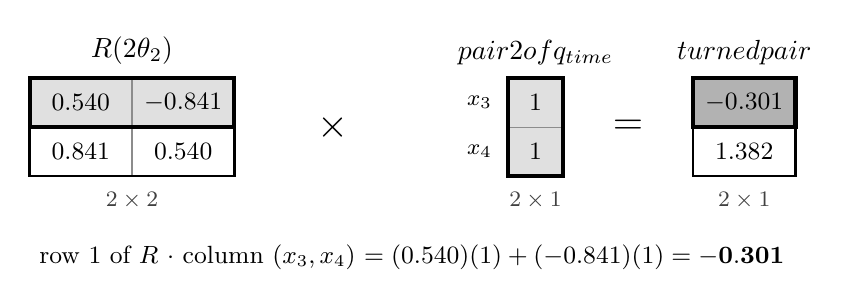
\begin{tikzpicture}
\draw[black!45, fill=black!12] (0.000,0.620) rectangle (1.300,0.000);
\node[font=\small, text=black] at (0.650,0.310) {$0.540$};
\draw[black!45, fill=black!12] (1.300,0.620) rectangle (2.600,0.000);
\node[font=\small, text=black] at (1.950,0.310) {$-0.841$};
\draw[black!45, fill=white] (0.000,0.000) rectangle (1.300,-0.620);
\node[font=\small, text=black] at (0.650,-0.310) {$0.841$};
\draw[black!45, fill=white] (1.300,0.000) rectangle (2.600,-0.620);
\node[font=\small, text=black] at (1.950,-0.310) {$0.540$};
\draw[line width=1.4pt] (0.000,0.620) rectangle (2.600,0.000);
\draw[line width=0.9pt] (0.000,0.620) rectangle (2.600,-0.620);
\node[anchor=south, font=\normalsize] at (1.300,0.670) {$R(2\theta_2)$};
\node[anchor=north, font=\footnotesize, text=black!75] at (1.300,-0.700) {$2\times2$};
\node[font=\Large] at (3.850,0) {$\times$};
\draw[black!45, fill=black!12] (6.075,0.620) rectangle (6.775,0.000);
\node[font=\small, text=black] at (6.425,0.310) {$1$};
\draw[black!45, fill=black!12] (6.075,0.000) rectangle (6.775,-0.620);
\node[font=\small, text=black] at (6.425,-0.310) {$1$};
\draw[line width=1.4pt] (6.075,0.620) rectangle (6.775,-0.620);
\draw[line width=0.9pt] (6.075,0.620) rectangle (6.775,-0.620);
\node[anchor=east, font=\footnotesize\ttfamily] at (5.995,0.310) {$x_3$};
\node[anchor=east, font=\footnotesize\ttfamily] at (5.995,-0.310) {$x_4$};
\node[anchor=south, font=\normalsize] at (6.425,0.670) {$\text{pair 2 of }\bm q_{\text{time}}$};
\node[anchor=north, font=\footnotesize, text=black!75] at (6.425,-0.700) {$2\times1$};
\node[font=\Large] at (7.600,0) {$=$};
\draw[black!45, fill=black!30] (8.425,0.620) rectangle (9.725,0.000);
\node[font=\small, text=black] at (9.075,0.310) {$-0.301$};
\draw[black!45, fill=white] (8.425,0.000) rectangle (9.725,-0.620);
\node[font=\small, text=black] at (9.075,-0.310) {$1.382$};
\draw[line width=1.6pt] (8.425,0.620) rectangle (9.725,0.000);
\draw[line width=0.9pt] (8.425,0.620) rectangle (9.725,-0.620);
\node[anchor=south, font=\normalsize] at (9.075,0.670) {$\text{turned pair}$};
\node[anchor=north, font=\footnotesize, text=black!75] at (9.075,-0.700) {$2\times1$};
\node[anchor=north west, font=\small, align=left] at (0,-1.370) {row 1 of $R$ $\cdot$ column $(x_3, x_4)$ $= (0.540)(1) + (-0.841)(1) = \mathbf{-0.301}$};
\end{tikzpicture}
}
\captionof{figure}{One turn, as a matrix product. Row 1 of the rotation matrix meets the pair $(x_3,x_4)=(1,1)$ and
gives the first number of the turned pair. The second row gives the second number the same way. The
pair's length is $\sqrt2$ before and after.}
\label{fig:ch4rot}
\end{center}

Only queries and keys are turned; values are left alone. Do the same for every pair of every row, each
row by its own position, and you get Figure~\ref{fig:ch4qk}. \tok{waste} sits at position 0, so its row is
not turned at all.

\begin{center}
\fitwidthFourFive{% AUTO-GENERATED by code/figlib.py helpers -- do not edit
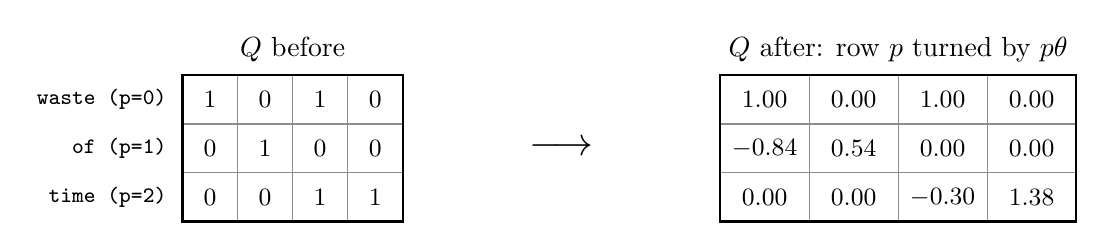
\begin{tikzpicture}
\draw[black!45, fill=white] (1.965,0.930) rectangle (2.665,0.310);
\node[font=\small, text=black] at (2.315,0.620) {$1$};
\draw[black!45, fill=white] (2.665,0.930) rectangle (3.365,0.310);
\node[font=\small, text=black] at (3.015,0.620) {$0$};
\draw[black!45, fill=white] (3.365,0.930) rectangle (4.065,0.310);
\node[font=\small, text=black] at (3.715,0.620) {$1$};
\draw[black!45, fill=white] (4.065,0.930) rectangle (4.765,0.310);
\node[font=\small, text=black] at (4.415,0.620) {$0$};
\draw[black!45, fill=white] (1.965,0.310) rectangle (2.665,-0.310);
\node[font=\small, text=black] at (2.315,-0.000) {$0$};
\draw[black!45, fill=white] (2.665,0.310) rectangle (3.365,-0.310);
\node[font=\small, text=black] at (3.015,-0.000) {$1$};
\draw[black!45, fill=white] (3.365,0.310) rectangle (4.065,-0.310);
\node[font=\small, text=black] at (3.715,-0.000) {$0$};
\draw[black!45, fill=white] (4.065,0.310) rectangle (4.765,-0.310);
\node[font=\small, text=black] at (4.415,-0.000) {$0$};
\draw[black!45, fill=white] (1.965,-0.310) rectangle (2.665,-0.930);
\node[font=\small, text=black] at (2.315,-0.620) {$0$};
\draw[black!45, fill=white] (2.665,-0.310) rectangle (3.365,-0.930);
\node[font=\small, text=black] at (3.015,-0.620) {$0$};
\draw[black!45, fill=white] (3.365,-0.310) rectangle (4.065,-0.930);
\node[font=\small, text=black] at (3.715,-0.620) {$1$};
\draw[black!45, fill=white] (4.065,-0.310) rectangle (4.765,-0.930);
\node[font=\small, text=black] at (4.415,-0.620) {$1$};
\draw[line width=0.9pt] (1.965,0.930) rectangle (4.765,-0.930);
\node[anchor=east, font=\footnotesize\ttfamily] at (1.885,0.620) {waste (p=0)};
\node[anchor=east, font=\footnotesize\ttfamily] at (1.885,-0.000) {of (p=1)};
\node[anchor=east, font=\footnotesize\ttfamily] at (1.885,-0.620) {time (p=2)};
\node[anchor=south, font=\normalsize] at (3.365,0.980) {$Q$ before};
\node[font=\Large] at (6.780,0) {$\longrightarrow$};
\draw[black!45, fill=white] (8.795,0.930) rectangle (9.925,0.310);
\node[font=\small, text=black] at (9.360,0.620) {$1.00$};
\draw[black!45, fill=white] (9.925,0.930) rectangle (11.055,0.310);
\node[font=\small, text=black] at (10.490,0.620) {$0.00$};
\draw[black!45, fill=white] (11.055,0.930) rectangle (12.185,0.310);
\node[font=\small, text=black] at (11.620,0.620) {$1.00$};
\draw[black!45, fill=white] (12.185,0.930) rectangle (13.315,0.310);
\node[font=\small, text=black] at (12.750,0.620) {$0.00$};
\draw[black!45, fill=white] (8.795,0.310) rectangle (9.925,-0.310);
\node[font=\small, text=black] at (9.360,-0.000) {$-0.84$};
\draw[black!45, fill=white] (9.925,0.310) rectangle (11.055,-0.310);
\node[font=\small, text=black] at (10.490,-0.000) {$0.54$};
\draw[black!45, fill=white] (11.055,0.310) rectangle (12.185,-0.310);
\node[font=\small, text=black] at (11.620,-0.000) {$0.00$};
\draw[black!45, fill=white] (12.185,0.310) rectangle (13.315,-0.310);
\node[font=\small, text=black] at (12.750,-0.000) {$0.00$};
\draw[black!45, fill=white] (8.795,-0.310) rectangle (9.925,-0.930);
\node[font=\small, text=black] at (9.360,-0.620) {$0.00$};
\draw[black!45, fill=white] (9.925,-0.310) rectangle (11.055,-0.930);
\node[font=\small, text=black] at (10.490,-0.620) {$0.00$};
\draw[black!45, fill=white] (11.055,-0.310) rectangle (12.185,-0.930);
\node[font=\small, text=black] at (11.620,-0.620) {$-0.30$};
\draw[black!45, fill=white] (12.185,-0.310) rectangle (13.315,-0.930);
\node[font=\small, text=black] at (12.750,-0.620) {$1.38$};
\draw[line width=0.9pt] (8.795,0.930) rectangle (13.315,-0.930);
\node[anchor=south, font=\normalsize] at (11.055,0.980) {$Q$ after: row $p$ turned by $p\theta$};
\end{tikzpicture}
\\[10pt]
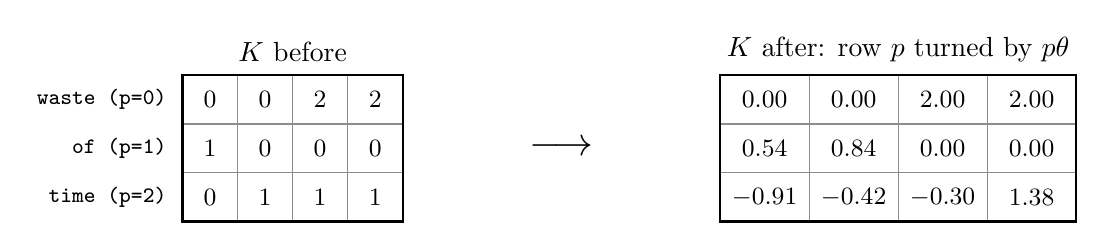
\begin{tikzpicture}
\draw[black!45, fill=white] (1.965,0.930) rectangle (2.665,0.310);
\node[font=\small, text=black] at (2.315,0.620) {$0$};
\draw[black!45, fill=white] (2.665,0.930) rectangle (3.365,0.310);
\node[font=\small, text=black] at (3.015,0.620) {$0$};
\draw[black!45, fill=white] (3.365,0.930) rectangle (4.065,0.310);
\node[font=\small, text=black] at (3.715,0.620) {$2$};
\draw[black!45, fill=white] (4.065,0.930) rectangle (4.765,0.310);
\node[font=\small, text=black] at (4.415,0.620) {$2$};
\draw[black!45, fill=white] (1.965,0.310) rectangle (2.665,-0.310);
\node[font=\small, text=black] at (2.315,-0.000) {$1$};
\draw[black!45, fill=white] (2.665,0.310) rectangle (3.365,-0.310);
\node[font=\small, text=black] at (3.015,-0.000) {$0$};
\draw[black!45, fill=white] (3.365,0.310) rectangle (4.065,-0.310);
\node[font=\small, text=black] at (3.715,-0.000) {$0$};
\draw[black!45, fill=white] (4.065,0.310) rectangle (4.765,-0.310);
\node[font=\small, text=black] at (4.415,-0.000) {$0$};
\draw[black!45, fill=white] (1.965,-0.310) rectangle (2.665,-0.930);
\node[font=\small, text=black] at (2.315,-0.620) {$0$};
\draw[black!45, fill=white] (2.665,-0.310) rectangle (3.365,-0.930);
\node[font=\small, text=black] at (3.015,-0.620) {$1$};
\draw[black!45, fill=white] (3.365,-0.310) rectangle (4.065,-0.930);
\node[font=\small, text=black] at (3.715,-0.620) {$1$};
\draw[black!45, fill=white] (4.065,-0.310) rectangle (4.765,-0.930);
\node[font=\small, text=black] at (4.415,-0.620) {$1$};
\draw[line width=0.9pt] (1.965,0.930) rectangle (4.765,-0.930);
\node[anchor=east, font=\footnotesize\ttfamily] at (1.885,0.620) {waste (p=0)};
\node[anchor=east, font=\footnotesize\ttfamily] at (1.885,-0.000) {of (p=1)};
\node[anchor=east, font=\footnotesize\ttfamily] at (1.885,-0.620) {time (p=2)};
\node[anchor=south, font=\normalsize] at (3.365,0.980) {$K$ before};
\node[font=\Large] at (6.780,0) {$\longrightarrow$};
\draw[black!45, fill=white] (8.795,0.930) rectangle (9.925,0.310);
\node[font=\small, text=black] at (9.360,0.620) {$0.00$};
\draw[black!45, fill=white] (9.925,0.930) rectangle (11.055,0.310);
\node[font=\small, text=black] at (10.490,0.620) {$0.00$};
\draw[black!45, fill=white] (11.055,0.930) rectangle (12.185,0.310);
\node[font=\small, text=black] at (11.620,0.620) {$2.00$};
\draw[black!45, fill=white] (12.185,0.930) rectangle (13.315,0.310);
\node[font=\small, text=black] at (12.750,0.620) {$2.00$};
\draw[black!45, fill=white] (8.795,0.310) rectangle (9.925,-0.310);
\node[font=\small, text=black] at (9.360,-0.000) {$0.54$};
\draw[black!45, fill=white] (9.925,0.310) rectangle (11.055,-0.310);
\node[font=\small, text=black] at (10.490,-0.000) {$0.84$};
\draw[black!45, fill=white] (11.055,0.310) rectangle (12.185,-0.310);
\node[font=\small, text=black] at (11.620,-0.000) {$0.00$};
\draw[black!45, fill=white] (12.185,0.310) rectangle (13.315,-0.310);
\node[font=\small, text=black] at (12.750,-0.000) {$0.00$};
\draw[black!45, fill=white] (8.795,-0.310) rectangle (9.925,-0.930);
\node[font=\small, text=black] at (9.360,-0.620) {$-0.91$};
\draw[black!45, fill=white] (9.925,-0.310) rectangle (11.055,-0.930);
\node[font=\small, text=black] at (10.490,-0.620) {$-0.42$};
\draw[black!45, fill=white] (11.055,-0.310) rectangle (12.185,-0.930);
\node[font=\small, text=black] at (11.620,-0.620) {$-0.30$};
\draw[black!45, fill=white] (12.185,-0.310) rectangle (13.315,-0.930);
\node[font=\small, text=black] at (12.750,-0.620) {$1.38$};
\draw[line width=0.9pt] (8.795,0.930) rectangle (13.315,-0.930);
\node[anchor=south, font=\normalsize] at (11.055,0.980) {$K$ after: row $p$ turned by $p\theta$};
\end{tikzpicture}
}
\captionof{figure}{Queries and keys of \tok{waste of time} before and after RoPE. Row $p$ is turned by $p$ times
$\theta$ (both of its pairs, each with its own speed). Row \tok{waste} ($p=0$) is unchanged.}
\label{fig:ch4qk}
\end{center}

\noindent Read the last row of $Q$ after turning: that is \tok{time}'s turned query. Now swap the first two words: \tok{waste}
moves to position 1, one step from \tok{time} instead of two. Figure~\ref{fig:ch4scores} shows the
whole score table $QK^\top$ (before scaling) for both orders, without and with RoPE.

\begin{center}
\fitwidthFourFive{% AUTO-GENERATED by code/figlib.py helpers -- do not edit
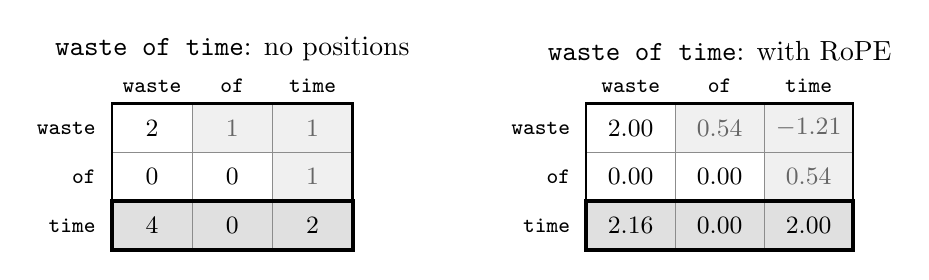
\begin{tikzpicture}
\draw[black!45, fill=white] (0.975,0.930) rectangle (1.995,0.310);
\node[font=\small, text=black] at (1.485,0.620) {$2$};
\draw[black!45, fill=black!6] (1.995,0.930) rectangle (3.015,0.310);
\node[font=\small, text=black!60] at (2.505,0.620) {$1$};
\draw[black!45, fill=black!6] (3.015,0.930) rectangle (4.035,0.310);
\node[font=\small, text=black!60] at (3.525,0.620) {$1$};
\draw[black!45, fill=white] (0.975,0.310) rectangle (1.995,-0.310);
\node[font=\small, text=black] at (1.485,-0.000) {$0$};
\draw[black!45, fill=white] (1.995,0.310) rectangle (3.015,-0.310);
\node[font=\small, text=black] at (2.505,-0.000) {$0$};
\draw[black!45, fill=black!6] (3.015,0.310) rectangle (4.035,-0.310);
\node[font=\small, text=black!60] at (3.525,-0.000) {$1$};
\draw[black!45, fill=black!12] (0.975,-0.310) rectangle (1.995,-0.930);
\node[font=\small, text=black] at (1.485,-0.620) {$4$};
\draw[black!45, fill=black!12] (1.995,-0.310) rectangle (3.015,-0.930);
\node[font=\small, text=black] at (2.505,-0.620) {$0$};
\draw[black!45, fill=black!12] (3.015,-0.310) rectangle (4.035,-0.930);
\node[font=\small, text=black] at (3.525,-0.620) {$2$};
\draw[line width=1.4pt] (0.975,-0.310) rectangle (4.035,-0.930);
\draw[line width=0.9pt] (0.975,0.930) rectangle (4.035,-0.930);
\node[anchor=east, font=\footnotesize\ttfamily] at (0.895,0.620) {waste};
\node[anchor=east, font=\footnotesize\ttfamily] at (0.895,-0.000) {of};
\node[anchor=east, font=\footnotesize\ttfamily] at (0.895,-0.620) {time};
\node[anchor=south, font=\footnotesize\ttfamily] at (1.485,0.950) {waste};
\node[anchor=south, font=\footnotesize\ttfamily] at (2.505,0.950) {of};
\node[anchor=south, font=\footnotesize\ttfamily] at (3.525,0.950) {time};
\node[anchor=south, font=\normalsize] at (2.505,1.350) {\texttt{waste of time}: no positions};
\node[font=\Large] at (5.030,0) {\quad};
\draw[black!45, fill=white] (7.000,0.930) rectangle (8.130,0.310);
\node[font=\small, text=black] at (7.565,0.620) {$2.00$};
\draw[black!45, fill=black!6] (8.130,0.930) rectangle (9.260,0.310);
\node[font=\small, text=black!60] at (8.695,0.620) {$0.54$};
\draw[black!45, fill=black!6] (9.260,0.930) rectangle (10.390,0.310);
\node[font=\small, text=black!60] at (9.825,0.620) {$-1.21$};
\draw[black!45, fill=white] (7.000,0.310) rectangle (8.130,-0.310);
\node[font=\small, text=black] at (7.565,-0.000) {$0.00$};
\draw[black!45, fill=white] (8.130,0.310) rectangle (9.260,-0.310);
\node[font=\small, text=black] at (8.695,-0.000) {$0.00$};
\draw[black!45, fill=black!6] (9.260,0.310) rectangle (10.390,-0.310);
\node[font=\small, text=black!60] at (9.825,-0.000) {$0.54$};
\draw[black!45, fill=black!12] (7.000,-0.310) rectangle (8.130,-0.930);
\node[font=\small, text=black] at (7.565,-0.620) {$2.16$};
\draw[black!45, fill=black!12] (8.130,-0.310) rectangle (9.260,-0.930);
\node[font=\small, text=black] at (8.695,-0.620) {$0.00$};
\draw[black!45, fill=black!12] (9.260,-0.310) rectangle (10.390,-0.930);
\node[font=\small, text=black] at (9.825,-0.620) {$2.00$};
\draw[line width=1.4pt] (7.000,-0.310) rectangle (10.390,-0.930);
\draw[line width=0.9pt] (7.000,0.930) rectangle (10.390,-0.930);
\node[anchor=east, font=\footnotesize\ttfamily] at (6.920,0.620) {waste};
\node[anchor=east, font=\footnotesize\ttfamily] at (6.920,-0.000) {of};
\node[anchor=east, font=\footnotesize\ttfamily] at (6.920,-0.620) {time};
\node[anchor=south, font=\footnotesize\ttfamily] at (7.565,0.950) {waste};
\node[anchor=south, font=\footnotesize\ttfamily] at (8.695,0.950) {of};
\node[anchor=south, font=\footnotesize\ttfamily] at (9.825,0.950) {time};
\node[anchor=south, font=\normalsize] at (8.695,1.350) {\texttt{waste of time}: with RoPE};
\end{tikzpicture}
\\[10pt]
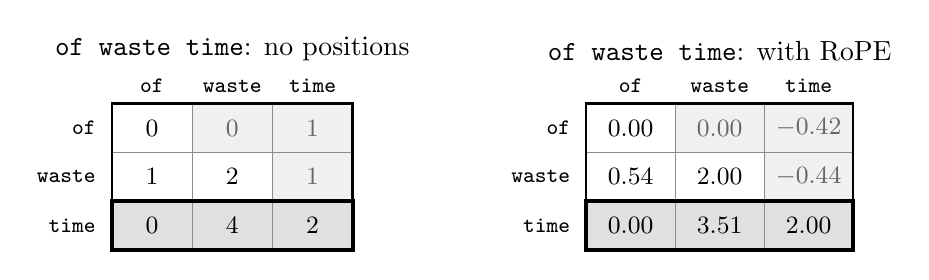
\begin{tikzpicture}
\draw[black!45, fill=white] (0.975,0.930) rectangle (1.995,0.310);
\node[font=\small, text=black] at (1.485,0.620) {$0$};
\draw[black!45, fill=black!6] (1.995,0.930) rectangle (3.015,0.310);
\node[font=\small, text=black!60] at (2.505,0.620) {$0$};
\draw[black!45, fill=black!6] (3.015,0.930) rectangle (4.035,0.310);
\node[font=\small, text=black!60] at (3.525,0.620) {$1$};
\draw[black!45, fill=white] (0.975,0.310) rectangle (1.995,-0.310);
\node[font=\small, text=black] at (1.485,-0.000) {$1$};
\draw[black!45, fill=white] (1.995,0.310) rectangle (3.015,-0.310);
\node[font=\small, text=black] at (2.505,-0.000) {$2$};
\draw[black!45, fill=black!6] (3.015,0.310) rectangle (4.035,-0.310);
\node[font=\small, text=black!60] at (3.525,-0.000) {$1$};
\draw[black!45, fill=black!12] (0.975,-0.310) rectangle (1.995,-0.930);
\node[font=\small, text=black] at (1.485,-0.620) {$0$};
\draw[black!45, fill=black!12] (1.995,-0.310) rectangle (3.015,-0.930);
\node[font=\small, text=black] at (2.505,-0.620) {$4$};
\draw[black!45, fill=black!12] (3.015,-0.310) rectangle (4.035,-0.930);
\node[font=\small, text=black] at (3.525,-0.620) {$2$};
\draw[line width=1.4pt] (0.975,-0.310) rectangle (4.035,-0.930);
\draw[line width=0.9pt] (0.975,0.930) rectangle (4.035,-0.930);
\node[anchor=east, font=\footnotesize\ttfamily] at (0.895,0.620) {of};
\node[anchor=east, font=\footnotesize\ttfamily] at (0.895,-0.000) {waste};
\node[anchor=east, font=\footnotesize\ttfamily] at (0.895,-0.620) {time};
\node[anchor=south, font=\footnotesize\ttfamily] at (1.485,0.950) {of};
\node[anchor=south, font=\footnotesize\ttfamily] at (2.505,0.950) {waste};
\node[anchor=south, font=\footnotesize\ttfamily] at (3.525,0.950) {time};
\node[anchor=south, font=\normalsize] at (2.505,1.350) {\texttt{of waste time}: no positions};
\node[font=\Large] at (5.030,0) {\quad};
\draw[black!45, fill=white] (7.000,0.930) rectangle (8.130,0.310);
\node[font=\small, text=black] at (7.565,0.620) {$0.00$};
\draw[black!45, fill=black!6] (8.130,0.930) rectangle (9.260,0.310);
\node[font=\small, text=black!60] at (8.695,0.620) {$0.00$};
\draw[black!45, fill=black!6] (9.260,0.930) rectangle (10.390,0.310);
\node[font=\small, text=black!60] at (9.825,0.620) {$-0.42$};
\draw[black!45, fill=white] (7.000,0.310) rectangle (8.130,-0.310);
\node[font=\small, text=black] at (7.565,-0.000) {$0.54$};
\draw[black!45, fill=white] (8.130,0.310) rectangle (9.260,-0.310);
\node[font=\small, text=black] at (8.695,-0.000) {$2.00$};
\draw[black!45, fill=black!6] (9.260,0.310) rectangle (10.390,-0.310);
\node[font=\small, text=black!60] at (9.825,-0.000) {$-0.44$};
\draw[black!45, fill=black!12] (7.000,-0.310) rectangle (8.130,-0.930);
\node[font=\small, text=black] at (7.565,-0.620) {$0.00$};
\draw[black!45, fill=black!12] (8.130,-0.310) rectangle (9.260,-0.930);
\node[font=\small, text=black] at (8.695,-0.620) {$3.51$};
\draw[black!45, fill=black!12] (9.260,-0.310) rectangle (10.390,-0.930);
\node[font=\small, text=black] at (9.825,-0.620) {$2.00$};
\draw[line width=1.4pt] (7.000,-0.310) rectangle (10.390,-0.930);
\draw[line width=0.9pt] (7.000,0.930) rectangle (10.390,-0.930);
\node[anchor=east, font=\footnotesize\ttfamily] at (6.920,0.620) {of};
\node[anchor=east, font=\footnotesize\ttfamily] at (6.920,-0.000) {waste};
\node[anchor=east, font=\footnotesize\ttfamily] at (6.920,-0.620) {time};
\node[anchor=south, font=\footnotesize\ttfamily] at (7.565,0.950) {of};
\node[anchor=south, font=\footnotesize\ttfamily] at (8.695,0.950) {waste};
\node[anchor=south, font=\footnotesize\ttfamily] at (9.825,0.950) {time};
\node[anchor=south, font=\normalsize] at (8.695,1.350) {\texttt{of waste time}: with RoPE};
\end{tikzpicture}
}
\captionof{figure}{Score tables for both word orders. Grey cells are covered by the causal mask. Compare the
outlined \tok{time} rows. Without positions they hold the same three numbers, only reordered: \tok{waste}
scores 4 wherever it stands. With RoPE \tok{waste}'s score depends on how far it is from \tok{time}.}
\label{fig:ch4scores}
\end{center}

\noindent For the query \tok{time}, after scaling and softmax:
\begin{center}
\small
\begin{tabular}{@{}l l l l@{}}
\toprule
order & dot products (before scaling) & shares after softmax & output $\bm{o}_{\text{time}}$\\
\midrule
\tok{waste of time} & $\nFourRopeScores$ & $\nFourRopeA$ & $\nFourRopeTime$\\
\tok{of waste time} & $\nFourRopeScoresSwap$ & $\nFourRopeASwap$ & $\nFourRopeTimeSwap$\\
\bottomrule
\end{tabular}
\end{center}
Each row lists the tokens in sentence order. \tok{waste}'s share goes from \nFourOrigWaste\ to
\nFourSwapWaste\ when it moves closer. Order now changes the answer, and nothing was added to any arrow:
the script checks that every turned arrow keeps its length.

\Exactly For a pair $(x_1, x_2)$ at position $p$, RoPE applies the rotation
\[
\begin{pmatrix} x_1' \\ x_2' \end{pmatrix} =
\begin{pmatrix} \cos p\theta & -\sin p\theta \\ \sin p\theta & \cos p\theta \end{pmatrix}
\begin{pmatrix} x_1 \\ x_2 \end{pmatrix},
\]
to every pair of every query and key, each pair with its own $\theta_i$. Write $R_p$ for this rotation.
Because turning by $m\theta$ and then measuring against something turned by $n\theta$ is the same as
turning by $(m-n)\theta$ alone,
\[
(R_m\bm{q})\cdot(R_n\bm{k}) \;=\; \bm{q}\cdot(R_{n-m}\bm{k}),
\]
which depends on $m$ and $n$ only through $m-n$. We checked this numerically on 1000 random queries and
keys of width 8 at random positions, shifting both positions by the same amount: the largest difference
in score was $\nFourRelWorst$, which is rounding error. In the toy, \tok{time} at position 2 looking at
\tok{waste} at 0 scores \nFourRelScore, and so does \tok{time} at 7 looking at \tok{waste} at 5.

\begin{wrongidea}{4.4}
``RoPE changes the token's embedding.'' It does not touch the embedding table or the values. It turns
the query and key after $W_Q$ and $W_K$ have made them, inside every attention layer, and it never changes
their length. What a token hands over (its value) is the same wherever it stands; only \emph{who finds
it} depends on distance.
\end{wrongidea}

\begin{checkq}
After RoPE, \tok{time} at position 2 and \tok{waste} at position 0 give a score of \nFourRelScore. What
score do they give at positions 12 and 10?
\begin{options}
\item \nFourRelScore, because only the distance (2) matters.
\item A larger score, because later words are turned more.
\item A score near 0, because the arrows have been turned so far that they no longer line up.
\item It cannot be known without recomputing the embeddings at the new positions.
\end{options}
\end{checkq}

\Why Rotation is the one operation that keeps lengths (so the scale of every score stays as Chapter 3
needs it, \S3.8) and turns ``two absolute positions'' into ``one distance'' for free. No table to learn, no
limit on length from a table, and no blending of word and badge.

\Summary{RoPE turns each pair of query and key coordinates by an angle proportional to position, so every
attention score depends only on how far apart the two tokens are.}

%---------------------------------------------------------------------
\subsection*{4.5\quad Many hands at different speeds}

\Predict A hand that turns \nFourDegOne$^\circ$ per word comes back to almost the same place after 44 words
($44$ radians is \nFourWrapTurns\ full turns). Could the model then confuse a word 44 tokens away with a
word in the same spot?

With one hand, yes. In the toy, the fast hand gives $\cos(44\theta_1) = \nFourWrapFast$, almost exactly
what distance 0 gives ($\cos 0 = 1$). But the slow hand turns $\theta_2 = \nFourThetaTwo$ per word, and
$\cos(44\theta_2) = \nFourWrapSlow$: completely different. Like the second, minute and hour hands of a
clock, each hand alone repeats, but together they pin down the distance. This is why $\theta_i$ is spread
over many speeds, from one turn every few tokens to one turn every many thousands.

\Exactly With head width 128 and base $b=10{,}000$, the slowest pair completes a turn only every
\nFourSlowWlTen\ positions. Long-context models raise the base: the published Qwen3 configuration
(Qwen3 technical report, 2025; to be checked against its \texttt{config.json} in Chapter 10) uses
$b=1{,}000{,}000$, which with head width 128 makes the slowest hand turn once every \nFourSlowWlMil\
positions.

\begin{breaks}
A clock tells the time of day exactly. Attention does not read the hands directly; it only sees the dot
product, which mixes all hands together, weighted by how much of the query and key sit in each pair. If a
query puts all its weight on the fast pairs, it effectively looks at short distances only. The model
learns where to put its weight.
\end{breaks}

\begin{wrongidea}{4.6}
``Rotations repeat, so a far word gets confused with a near one.'' Each hand repeats, the set of hands
does not, over the lengths the model is built for. Past the slowest hand's turn the guarantee weakens,
which is one reason models have a maximum context length.
\end{wrongidea}

\begin{checkq}
Why does RoPE use many different speeds $\theta_i$ instead of one?
\begin{options}
\item One speed would make every word at a multiple of the repeat distance look as if it were at distance 0.
\item Different speeds make the arrows longer.
\item Each speed stores the absolute position of one word.
\item More speeds mean the values can be rotated too.
\end{options}
\end{checkq}

\Summary{fast hands separate neighbours, slow hands separate distant words, and together they make
distances distinguishable over long texts.}

%---------------------------------------------------------------------
\subsection*{4.6\quad What we built}

\begin{principle}{encode relationships, not coordinates}
RoPE works because it stores what the task needs (a distance) rather than what is easy to write down (an
absolute index). The same move pays off in system design. A memory system that stores ``three messages
ago the user said X'' survives the conversation getting longer; one that stores ``message 17 said X'' has
to be fixed every time messages are inserted. When you design a feature, ask: is my model asked to
compare things, and am I giving it the comparison or two raw positions to subtract?
\end{principle}

\begin{lookingback}
(a) In \S3.2, the dot product has two knobs. Which one does RoPE leave alone, and which one does it
change? (b) Why does \S3.8's division by $\sqrt{d_k}$ still work after RoPE? (c) Which requirement from
Chapter 1 did Chapter 3 lose and this chapter restore?
\end{lookingback}

%---------------------------------------------------------------------
\subsection*{Exercises}

\begin{exercise}
Turn the arrow $(1,0)$ by $90^\circ$ and the arrow $(0,1)$ by $90^\circ$. What is the dot product before
and after? Explain in one sentence why this is the heart of RoPE.
\end{exercise}

\begin{exercise}
In the toy with $b=4$, the first hand turns 1 radian per position. How many positions does it take to
come back close to where it started? Why could that matter for a 30-word support message?
\end{exercise}

\begin{exercise}
GPT-2 learned one position vector per position for 1024 positions, each of width 768. How many numbers
is that table? What happens when a text has 1025 tokens?
\end{exercise}

\begin{exercise}
A colleague says: ``With sinusoidal badges, the model knows absolute position; with RoPE, it knows only
relative position. So RoPE loses information.'' What would you answer? Use the support reply as your
example.
\end{exercise}

%---------------------------------------------------------------------
\subsection*{Answers to Chapter 4}

\noindent\textbf{Check yourself 4.1.} (a). Both positions moved by 10, the distance is still 2, and the
score depends only on the distance. (b) and (c) treat RoPE as tied to absolute position (M4.5); (d)
reflects M4.4, since the embeddings are never changed.

\noindent\textbf{Check yourself 4.2.} (a). With a single speed, distances that differ by a whole number of
turns look the same (M4.6 is the over-reaction to this). (b) is wrong because rotation keeps lengths;
(c) is M4.5; (d) is M4.4, values are never rotated.

\noindent\textbf{Looking back.} (a) It leaves the lengths alone and changes the angle. (b) Rotation keeps
each arrow's length, so dot products keep the same typical size and the same $\sqrt{d_k}$ applies.
(c) Requirement 2: knowing which word came where.

\noindent\textbf{Exercise 4.1.} Before: $(1,0)\cdot(0,1)=0$. After: $(0,1)\cdot(-1,0)=0$. Turning both
arrows by the same angle leaves their angle, and so their dot product, unchanged: only the
\emph{difference} in turning can change a score.

\noindent\textbf{Exercise 4.2.} One full turn is $2\pi\approx\nFourTwoPi$ radians, so a little more than every 6 positions, and
it is close to a full turn after 44 (\nFourWrapTurns\ turns). In a 30-word message, the fast hand alone
would mix up some distances; the slower hand (\nFourThetaTwo\ radians per word, a turn every \nFourToySlowWl\ words) separates
them. With only two hands the toy is still limited; real models have one hand per pair of coordinates, 64 per head for head width 128.

\noindent\textbf{Exercise 4.3.} $1024\times768 = \nFourGptPosTable$ numbers. A 1025th token has no row, so the model
cannot process it without extending and re-training the table.

\noindent\textbf{Exercise 4.4.} For the reply, what matters is that \tok{Sorry} comes right after the
complaint, not that the complaint started at word 340 of the chat. Relative position is what the task
needs. Absolute position can still be recovered where it matters (for example, through the distance to
the first token of the text). In practice, most current open models, including Llama (Touvron and
colleagues, 2023) and Qwen3, use RoPE, which suggests little that matters is lost.

\paragraph{What you now know.}
\begin{itemize}
\item Why attention needs help with order, shown with the swap test.
\item The three historical fixes: learned position vectors, sinusoidal waves, and rotation (RoPE).
\item Why rotation makes every score depend only on distance, checked numerically.
\item Why many rotation speeds are needed, and what raising the base does for long texts.
\end{itemize}

\clearpage\newpage
\section*{5\quad Many heads, the MLP, the residual stream}
\addcontentsline{toc}{section}{5 Many heads, the MLP, the residual stream}
\startchapter{5}
\ifdefined\fitwidthFourFive\else
\newsavebox{\fitboxFourFive}
\newcommand{\fitwidthFourFive}[1]{\sbox{\fitboxFourFive}{\begin{tabular}{@{}c@{}}#1\end{tabular}}\ifdim\wd\fitboxFourFive>\linewidth\resizebox{\linewidth}{!}{\usebox{\fitboxFourFive}}\else\usebox{\fitboxFourFive}\fi}
\fi

\begin{chaptermap}
\emph{The problem:} one attention head lets \tok{time} look back, but it can only ask one question at a time,
and nothing yet lets a token \emph{think} about what it heard. \emph{The steps:} see why one head blurs two
answers into one (\S5.1); split the width into two heads that ask different questions (\S5.2); stitch their
answers back together (\S5.3); give each token a private checklist of patterns, the MLP (\S5.4); and keep
every layer's work on a shared notebook, the residual stream (\S5.5). \emph{Where it ends:} with one complete
transformer block that, on our three tokens, predicts \tok{of} after \tok{waste}, \tok{time} after \tok{of}
and \tok{Sorry} after \tok{time}, all in one pass.
\end{chaptermap}

\machine{5}{You are here: Chapter 5 turns the single attention head into several heads, adds the MLP
(each token thinks alone), and adds the two $+$ circles of the residual stream. With these, the dashed
frame becomes one complete layer, which a real model repeats $L$ times. The norms are still ahead
(Chapter 6).}

\begin{beforeyoustart}
Five quick questions. Answer each, then read the refresher under it.
\begin{enumerate}[label=\arabic*.,leftmargin=1.6em]
\item Add the arrows $(1,2)$ and $(3,-1)$.\\
\emph{Refresher:} add matching entries: $(1+3,\ 2-1)=(4,1)$. On paper, put the second arrow's tail on the
first arrow's head.
\item What is the average of the arrows $(1,1,0,0)$ and $(0,0,0,1)$?\\
\emph{Refresher:} add them and halve every entry: $(0.5, 0.5, 0, 0.5)$.
\item Write the list $(2,1)$ followed by the list $(3,4)$ as one list.\\
\emph{Refresher:} placing lists end to end is called \emph{concatenating}: $(2,1,3,4)$.
\item What is the larger of $0$ and $-1.5$? Of $0$ and $\nFiveNThreeTime$?\\
\emph{Refresher:} the function $\max(0, x)$ keeps positive numbers and turns negative ones into 0. Here: $0$
and $\nFiveNThreeTime$.
\item In Chapter 3, how much of its attention did \tok{time} give to \tok{waste}?\\
\emph{Refresher:} \nFiveChThreeWaste\%, and \nFiveChThreeOf\% to \tok{of}. If that number is hazy, reread \S3.6
before going on.
\end{enumerate}
\end{beforeyoustart}

%---------------------------------------------------------------------
\subsection*{5.1\quad One head, one blurred answer}

\Predict In Chapter 3, one head computed \emph{one} set of shares for \tok{time}, and handed back \emph{one}
blend of value arrows. Suppose \tok{time} needs two different things: the judgement in \tok{waste}, and the
fact that \tok{of} sits right before it. Can one blend carry both, and keep them apart? Make a guess before
reading on.

\Picture Two colleagues report to you at the same moment, into the same microphone. You hear one mixed sound.
You can tell that two people spoke, but you cannot tell who said what.

\Exactly Take the value arrows of Chapter 3 for \tok{waste} and \tok{of}. A head that splits its
attention evenly hands back half of one plus half of the other, entry by entry (top row of
Figure~\ref{fig:ch5blend}). Now take two \emph{different} value arrows (bottom row). Their even blend is
the same arrow. Our script checks this.

\begin{center}
\fitwidthFourFive{% AUTO-GENERATED by code/figlib.py helpers -- do not edit
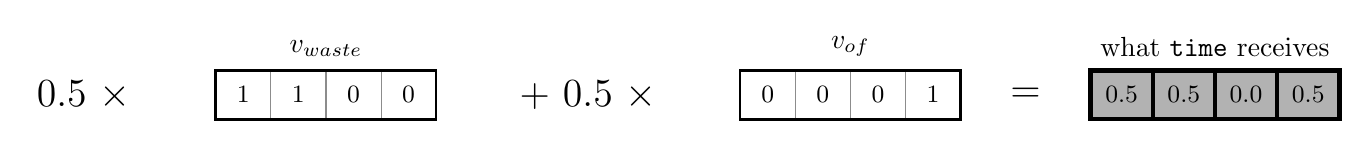
\begin{tikzpicture}
\node[font=\Large] at (1.255,0) {$0.5\ \times$};
\draw[black!45, fill=white] (2.930,0.310) rectangle (3.630,-0.310);
\node[font=\small, text=black] at (3.280,0.000) {$1$};
\draw[black!45, fill=white] (3.630,0.310) rectangle (4.330,-0.310);
\node[font=\small, text=black] at (3.980,0.000) {$1$};
\draw[black!45, fill=white] (4.330,0.310) rectangle (5.030,-0.310);
\node[font=\small, text=black] at (4.680,0.000) {$0$};
\draw[black!45, fill=white] (5.030,0.310) rectangle (5.730,-0.310);
\node[font=\small, text=black] at (5.380,0.000) {$0$};
\draw[line width=0.9pt] (2.930,0.310) rectangle (5.730,-0.310);
\node[anchor=south, font=\normalsize] at (4.330,0.360) {$\bm v_{\text{waste}}$};
\node[font=\Large] at (7.660,0) {$+\ 0.5\ \times$};
\draw[black!45, fill=white] (9.590,0.310) rectangle (10.290,-0.310);
\node[font=\small, text=black] at (9.940,0.000) {$0$};
\draw[black!45, fill=white] (10.290,0.310) rectangle (10.990,-0.310);
\node[font=\small, text=black] at (10.640,0.000) {$0$};
\draw[black!45, fill=white] (10.990,0.310) rectangle (11.690,-0.310);
\node[font=\small, text=black] at (11.340,0.000) {$0$};
\draw[black!45, fill=white] (11.690,0.310) rectangle (12.390,-0.310);
\node[font=\small, text=black] at (12.040,0.000) {$1$};
\draw[line width=0.9pt] (9.590,0.310) rectangle (12.390,-0.310);
\node[anchor=south, font=\normalsize] at (10.990,0.360) {$\bm v_{\text{of}}$};
\node[font=\Large] at (13.215,0) {$=$};
\draw[black!45, fill=black!30] (14.040,0.310) rectangle (14.830,-0.310);
\node[font=\small, text=black] at (14.435,0.000) {$0.5$};
\draw[black!45, fill=black!30] (14.830,0.310) rectangle (15.620,-0.310);
\node[font=\small, text=black] at (15.225,0.000) {$0.5$};
\draw[black!45, fill=black!30] (15.620,0.310) rectangle (16.410,-0.310);
\node[font=\small, text=black] at (16.015,0.000) {$0.0$};
\draw[black!45, fill=black!30] (16.410,0.310) rectangle (17.200,-0.310);
\node[font=\small, text=black] at (16.805,0.000) {$0.5$};
\draw[line width=1.6pt] (14.040,0.310) rectangle (14.830,-0.310);
\draw[line width=1.6pt] (14.830,0.310) rectangle (15.620,-0.310);
\draw[line width=1.6pt] (15.620,0.310) rectangle (16.410,-0.310);
\draw[line width=1.6pt] (16.410,0.310) rectangle (17.200,-0.310);
\draw[line width=0.9pt] (14.040,0.310) rectangle (17.200,-0.310);
\node[anchor=south, font=\normalsize] at (15.620,0.360) {what \texttt{time} receives};
\end{tikzpicture}
\\[10pt]
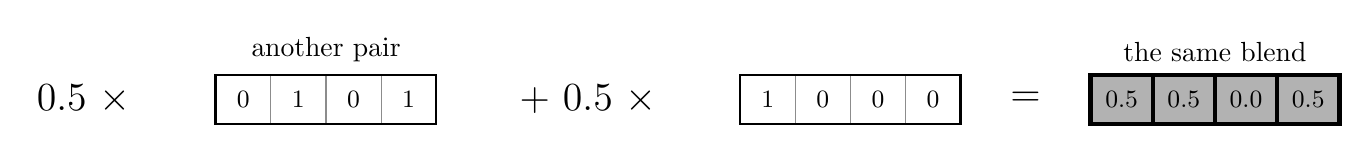
\begin{tikzpicture}
\node[font=\Large] at (1.255,0) {$0.5\ \times$};
\draw[black!45, fill=white] (2.930,0.310) rectangle (3.630,-0.310);
\node[font=\small, text=black] at (3.280,0.000) {$0$};
\draw[black!45, fill=white] (3.630,0.310) rectangle (4.330,-0.310);
\node[font=\small, text=black] at (3.980,0.000) {$1$};
\draw[black!45, fill=white] (4.330,0.310) rectangle (5.030,-0.310);
\node[font=\small, text=black] at (4.680,0.000) {$0$};
\draw[black!45, fill=white] (5.030,0.310) rectangle (5.730,-0.310);
\node[font=\small, text=black] at (5.380,0.000) {$1$};
\draw[line width=0.9pt] (2.930,0.310) rectangle (5.730,-0.310);
\node[anchor=south, font=\normalsize] at (4.330,0.360) {another pair};
\node[font=\Large] at (7.660,0) {$+\ 0.5\ \times$};
\draw[black!45, fill=white] (9.590,0.310) rectangle (10.290,-0.310);
\node[font=\small, text=black] at (9.940,0.000) {$1$};
\draw[black!45, fill=white] (10.290,0.310) rectangle (10.990,-0.310);
\node[font=\small, text=black] at (10.640,0.000) {$0$};
\draw[black!45, fill=white] (10.990,0.310) rectangle (11.690,-0.310);
\node[font=\small, text=black] at (11.340,0.000) {$0$};
\draw[black!45, fill=white] (11.690,0.310) rectangle (12.390,-0.310);
\node[font=\small, text=black] at (12.040,0.000) {$0$};
\draw[line width=0.9pt] (9.590,0.310) rectangle (12.390,-0.310);
\node[anchor=south, font=\normalsize] at (10.990,0.360) {\phantom{p}};
\node[font=\Large] at (13.215,0) {$=$};
\draw[black!45, fill=black!30] (14.040,0.310) rectangle (14.830,-0.310);
\node[font=\small, text=black] at (14.435,0.000) {$0.5$};
\draw[black!45, fill=black!30] (14.830,0.310) rectangle (15.620,-0.310);
\node[font=\small, text=black] at (15.225,0.000) {$0.5$};
\draw[black!45, fill=black!30] (15.620,0.310) rectangle (16.410,-0.310);
\node[font=\small, text=black] at (16.015,0.000) {$0.0$};
\draw[black!45, fill=black!30] (16.410,0.310) rectangle (17.200,-0.310);
\node[font=\small, text=black] at (16.805,0.000) {$0.5$};
\draw[line width=1.6pt] (14.040,0.310) rectangle (14.830,-0.310);
\draw[line width=1.6pt] (14.830,0.310) rectangle (15.620,-0.310);
\draw[line width=1.6pt] (15.620,0.310) rectangle (16.410,-0.310);
\draw[line width=1.6pt] (16.410,0.310) rectangle (17.200,-0.310);
\draw[line width=0.9pt] (14.040,0.310) rectangle (17.200,-0.310);
\node[anchor=south, font=\normalsize] at (15.620,0.360) {the same blend};
\end{tikzpicture}
}
\captionof{figure}{One head, one blend. Top: half of $\bm{v}_{\text{waste}}$ plus half of $\bm{v}_{\text{of}}$, entry by entry. Bottom: a different pair of arrows gives exactly the same shaded result, so the result alone cannot say who said what.}
\label{fig:ch5blend}
\end{center}
 Two different pairs of reports, one identical blend: after the
averaging, the token cannot know which pair it heard. A weighted average is a single arrow, and a single
arrow can be built from many different mixtures.

\begin{breaks}
The microphone picture suggests the information is gone for good. In a trained model the value arrows are
learned, and they can be made to point in separate directions so that a blend is still readable. The real
limit is that one head has one set of shares: it must decide how much \tok{waste} matters and how much
\tok{of} matters with a single softmax, so emphasising one always takes attention from the other.
\end{breaks}

\Why A softmax hands out shares that add to 1. So within one head, attention is a fixed budget, and every
question competes for it. To ask two questions without competition, you need two budgets.

\begin{wrongidea}{5.2}
\emph{One head can attend to two tokens equally well, by giving each 50\%.} It can attend to both, but it
cannot keep their messages apart, and it cannot make one share bigger without shrinking the other. That is
the difference between ``listening to two people'' and ``hearing two people talk at once''.
\end{wrongidea}

\begin{checkq}
A single head gives \tok{time} the shares $(0.5, 0.5, 0)$ over \tok{waste}, \tok{of}, \tok{time}. What can
\tok{time} tell from the output alone?
\begin{options}
\item Exactly what \tok{waste} said and exactly what \tok{of} said.
\item The average of what they said, but not which part came from whom.
\item Nothing at all, because averages destroy everything.
\item What \tok{time} itself said, since it always attends to itself.
\end{options}
\end{checkq}

\Summary{One head returns one weighted average, so asking two questions needs two heads.}

%---------------------------------------------------------------------
\subsection*{5.2\quad Two heads, each half as wide}

\Picture Instead of one reporter who listens to everyone, send two reporters with different briefs. One is
told ``find any judgement nearby''. The other is told ``find the small linking words''. Each writes a short
note.

The budget does not grow. Our arrows still have $d=4$ numbers, so the two heads get $d_k=2$ each. In the
same way, a model with width 64 and two heads gives each head 32 recipes. Each head is narrower, and in exchange there are more of them.

\paragraph{Worked example: head 1, fully.} Head 1 has its own three machines, each $4\times2$ (four
numbers in, two out):
\[
W_Q^{(1)}=\nFiveWQone,\quad W_K^{(1)}=\nFiveWKone,\quad W_V^{(1)}=\nFiveWVone \shape{d\times d_k=4\times2}
\]
Figure~\ref{fig:ch5headone} does the three products. In each one, the outlined row meets the outlined
column, and the dark cell is the number they make.

\begin{center}
\fitwidthFourFive{% AUTO-GENERATED by code/figlib.py helpers -- do not edit
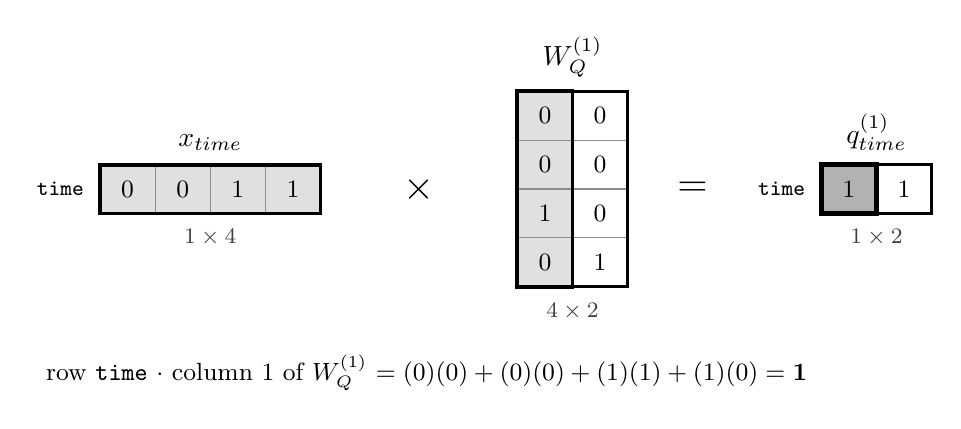
\begin{tikzpicture}
\draw[black!45, fill=black!12] (0.810,0.310) rectangle (1.510,-0.310);
\node[font=\small, text=black] at (1.160,0.000) {$0$};
\draw[black!45, fill=black!12] (1.510,0.310) rectangle (2.210,-0.310);
\node[font=\small, text=black] at (1.860,0.000) {$0$};
\draw[black!45, fill=black!12] (2.210,0.310) rectangle (2.910,-0.310);
\node[font=\small, text=black] at (2.560,0.000) {$1$};
\draw[black!45, fill=black!12] (2.910,0.310) rectangle (3.610,-0.310);
\node[font=\small, text=black] at (3.260,0.000) {$1$};
\draw[line width=1.4pt] (0.810,0.310) rectangle (3.610,-0.310);
\draw[line width=0.9pt] (0.810,0.310) rectangle (3.610,-0.310);
\node[anchor=east, font=\footnotesize\ttfamily] at (0.730,0.000) {time};
\node[anchor=south, font=\normalsize] at (2.210,0.360) {$\bm x_{\text{time}}$};
\node[anchor=north, font=\footnotesize, text=black!75] at (2.210,-0.390) {$1\times4$};
\node[font=\Large] at (4.860,0) {$\times$};
\draw[black!45, fill=black!12] (6.110,1.240) rectangle (6.810,0.620);
\node[font=\small, text=black] at (6.460,0.930) {$0$};
\draw[black!45, fill=white] (6.810,1.240) rectangle (7.510,0.620);
\node[font=\small, text=black] at (7.160,0.930) {$0$};
\draw[black!45, fill=black!12] (6.110,0.620) rectangle (6.810,0.000);
\node[font=\small, text=black] at (6.460,0.310) {$0$};
\draw[black!45, fill=white] (6.810,0.620) rectangle (7.510,0.000);
\node[font=\small, text=black] at (7.160,0.310) {$0$};
\draw[black!45, fill=black!12] (6.110,0.000) rectangle (6.810,-0.620);
\node[font=\small, text=black] at (6.460,-0.310) {$1$};
\draw[black!45, fill=white] (6.810,0.000) rectangle (7.510,-0.620);
\node[font=\small, text=black] at (7.160,-0.310) {$0$};
\draw[black!45, fill=black!12] (6.110,-0.620) rectangle (6.810,-1.240);
\node[font=\small, text=black] at (6.460,-0.930) {$0$};
\draw[black!45, fill=white] (6.810,-0.620) rectangle (7.510,-1.240);
\node[font=\small, text=black] at (7.160,-0.930) {$1$};
\draw[line width=1.4pt] (6.110,1.240) rectangle (6.810,-1.240);
\draw[line width=0.9pt] (6.110,1.240) rectangle (7.510,-1.240);
\node[anchor=south, font=\normalsize] at (6.810,1.290) {$W_Q^{(1)}$};
\node[anchor=north, font=\footnotesize, text=black!75] at (6.810,-1.320) {$4\times2$};
\node[font=\Large] at (8.335,0) {$=$};
\draw[black!45, fill=black!30] (9.970,0.310) rectangle (10.670,-0.310);
\node[font=\small, text=black] at (10.320,0.000) {$1$};
\draw[black!45, fill=white] (10.670,0.310) rectangle (11.370,-0.310);
\node[font=\small, text=black] at (11.020,0.000) {$1$};
\draw[line width=1.6pt] (9.970,0.310) rectangle (10.670,-0.310);
\draw[line width=0.9pt] (9.970,0.310) rectangle (11.370,-0.310);
\node[anchor=east, font=\footnotesize\ttfamily] at (9.890,0.000) {time};
\node[anchor=south, font=\normalsize] at (10.670,0.360) {$\bm q^{(1)}_{\text{time}}$};
\node[anchor=north, font=\footnotesize, text=black!75] at (10.670,-0.390) {$1\times2$};
\node[anchor=north west, font=\small, align=left] at (0,-1.990) {row \texttt{time} $\cdot$ column 1 of $W_Q^{(1)}$ $= (0)(0) + (0)(0) + (1)(1) + (1)(0) = \mathbf{1}$};
\end{tikzpicture}
\\[10pt]
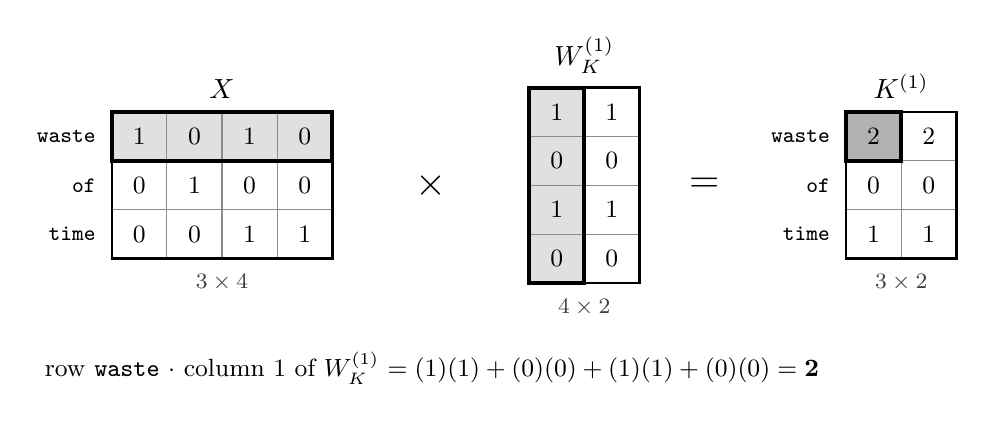
\begin{tikzpicture}
\draw[black!45, fill=black!12] (0.975,0.930) rectangle (1.675,0.310);
\node[font=\small, text=black] at (1.325,0.620) {$1$};
\draw[black!45, fill=black!12] (1.675,0.930) rectangle (2.375,0.310);
\node[font=\small, text=black] at (2.025,0.620) {$0$};
\draw[black!45, fill=black!12] (2.375,0.930) rectangle (3.075,0.310);
\node[font=\small, text=black] at (2.725,0.620) {$1$};
\draw[black!45, fill=black!12] (3.075,0.930) rectangle (3.775,0.310);
\node[font=\small, text=black] at (3.425,0.620) {$0$};
\draw[black!45, fill=white] (0.975,0.310) rectangle (1.675,-0.310);
\node[font=\small, text=black] at (1.325,-0.000) {$0$};
\draw[black!45, fill=white] (1.675,0.310) rectangle (2.375,-0.310);
\node[font=\small, text=black] at (2.025,-0.000) {$1$};
\draw[black!45, fill=white] (2.375,0.310) rectangle (3.075,-0.310);
\node[font=\small, text=black] at (2.725,-0.000) {$0$};
\draw[black!45, fill=white] (3.075,0.310) rectangle (3.775,-0.310);
\node[font=\small, text=black] at (3.425,-0.000) {$0$};
\draw[black!45, fill=white] (0.975,-0.310) rectangle (1.675,-0.930);
\node[font=\small, text=black] at (1.325,-0.620) {$0$};
\draw[black!45, fill=white] (1.675,-0.310) rectangle (2.375,-0.930);
\node[font=\small, text=black] at (2.025,-0.620) {$0$};
\draw[black!45, fill=white] (2.375,-0.310) rectangle (3.075,-0.930);
\node[font=\small, text=black] at (2.725,-0.620) {$1$};
\draw[black!45, fill=white] (3.075,-0.310) rectangle (3.775,-0.930);
\node[font=\small, text=black] at (3.425,-0.620) {$1$};
\draw[line width=1.4pt] (0.975,0.930) rectangle (3.775,0.310);
\draw[line width=0.9pt] (0.975,0.930) rectangle (3.775,-0.930);
\node[anchor=east, font=\footnotesize\ttfamily] at (0.895,0.620) {waste};
\node[anchor=east, font=\footnotesize\ttfamily] at (0.895,-0.000) {of};
\node[anchor=east, font=\footnotesize\ttfamily] at (0.895,-0.620) {time};
\node[anchor=south, font=\normalsize] at (2.375,0.980) {$X$};
\node[anchor=north, font=\footnotesize, text=black!75] at (2.375,-1.010) {$3\times4$};
\node[font=\Large] at (5.025,0) {$\times$};
\draw[black!45, fill=black!12] (6.275,1.240) rectangle (6.975,0.620);
\node[font=\small, text=black] at (6.625,0.930) {$1$};
\draw[black!45, fill=white] (6.975,1.240) rectangle (7.675,0.620);
\node[font=\small, text=black] at (7.325,0.930) {$1$};
\draw[black!45, fill=black!12] (6.275,0.620) rectangle (6.975,0.000);
\node[font=\small, text=black] at (6.625,0.310) {$0$};
\draw[black!45, fill=white] (6.975,0.620) rectangle (7.675,0.000);
\node[font=\small, text=black] at (7.325,0.310) {$0$};
\draw[black!45, fill=black!12] (6.275,0.000) rectangle (6.975,-0.620);
\node[font=\small, text=black] at (6.625,-0.310) {$1$};
\draw[black!45, fill=white] (6.975,0.000) rectangle (7.675,-0.620);
\node[font=\small, text=black] at (7.325,-0.310) {$1$};
\draw[black!45, fill=black!12] (6.275,-0.620) rectangle (6.975,-1.240);
\node[font=\small, text=black] at (6.625,-0.930) {$0$};
\draw[black!45, fill=white] (6.975,-0.620) rectangle (7.675,-1.240);
\node[font=\small, text=black] at (7.325,-0.930) {$0$};
\draw[line width=1.4pt] (6.275,1.240) rectangle (6.975,-1.240);
\draw[line width=0.9pt] (6.275,1.240) rectangle (7.675,-1.240);
\node[anchor=south, font=\normalsize] at (6.975,1.290) {$W_K^{(1)}$};
\node[anchor=north, font=\footnotesize, text=black!75] at (6.975,-1.320) {$4\times2$};
\node[font=\Large] at (8.500,0) {$=$};
\draw[black!45, fill=black!30] (10.300,0.930) rectangle (11.000,0.310);
\node[font=\small, text=black] at (10.650,0.620) {$2$};
\draw[black!45, fill=white] (11.000,0.930) rectangle (11.700,0.310);
\node[font=\small, text=black] at (11.350,0.620) {$2$};
\draw[black!45, fill=white] (10.300,0.310) rectangle (11.000,-0.310);
\node[font=\small, text=black] at (10.650,-0.000) {$0$};
\draw[black!45, fill=white] (11.000,0.310) rectangle (11.700,-0.310);
\node[font=\small, text=black] at (11.350,-0.000) {$0$};
\draw[black!45, fill=white] (10.300,-0.310) rectangle (11.000,-0.930);
\node[font=\small, text=black] at (10.650,-0.620) {$1$};
\draw[black!45, fill=white] (11.000,-0.310) rectangle (11.700,-0.930);
\node[font=\small, text=black] at (11.350,-0.620) {$1$};
\draw[line width=1.6pt] (10.300,0.930) rectangle (11.000,0.310);
\draw[line width=0.9pt] (10.300,0.930) rectangle (11.700,-0.930);
\node[anchor=east, font=\footnotesize\ttfamily] at (10.220,0.620) {waste};
\node[anchor=east, font=\footnotesize\ttfamily] at (10.220,-0.000) {of};
\node[anchor=east, font=\footnotesize\ttfamily] at (10.220,-0.620) {time};
\node[anchor=south, font=\normalsize] at (11.000,0.980) {$K^{(1)}$};
\node[anchor=north, font=\footnotesize, text=black!75] at (11.000,-1.010) {$3\times2$};
\node[anchor=north west, font=\small, align=left] at (0,-1.990) {row \texttt{waste} $\cdot$ column 1 of $W_K^{(1)}$ $= (1)(1) + (0)(0) + (1)(1) + (0)(0) = \mathbf{2}$};
\end{tikzpicture}
\\[10pt]
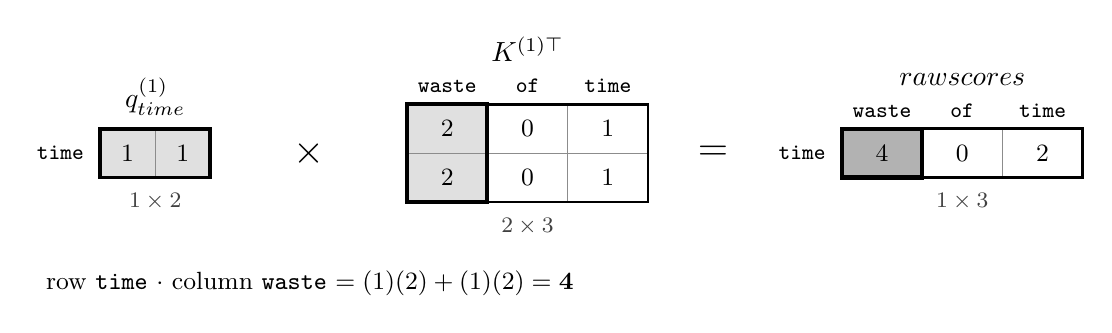
\begin{tikzpicture}
\draw[black!45, fill=black!12] (0.810,0.310) rectangle (1.510,-0.310);
\node[font=\small, text=black] at (1.160,0.000) {$1$};
\draw[black!45, fill=black!12] (1.510,0.310) rectangle (2.210,-0.310);
\node[font=\small, text=black] at (1.860,0.000) {$1$};
\draw[line width=1.4pt] (0.810,0.310) rectangle (2.210,-0.310);
\draw[line width=0.9pt] (0.810,0.310) rectangle (2.210,-0.310);
\node[anchor=east, font=\footnotesize\ttfamily] at (0.730,0.000) {time};
\node[anchor=south, font=\normalsize] at (1.510,0.360) {$\bm q^{(1)}_{\text{time}}$};
\node[anchor=north, font=\footnotesize, text=black!75] at (1.510,-0.390) {$1\times2$};
\node[font=\Large] at (3.460,0) {$\times$};
\draw[black!45, fill=black!12] (4.710,0.620) rectangle (5.730,0.000);
\node[font=\small, text=black] at (5.220,0.310) {$2$};
\draw[black!45, fill=white] (5.730,0.620) rectangle (6.750,0.000);
\node[font=\small, text=black] at (6.240,0.310) {$0$};
\draw[black!45, fill=white] (6.750,0.620) rectangle (7.770,0.000);
\node[font=\small, text=black] at (7.260,0.310) {$1$};
\draw[black!45, fill=black!12] (4.710,0.000) rectangle (5.730,-0.620);
\node[font=\small, text=black] at (5.220,-0.310) {$2$};
\draw[black!45, fill=white] (5.730,0.000) rectangle (6.750,-0.620);
\node[font=\small, text=black] at (6.240,-0.310) {$0$};
\draw[black!45, fill=white] (6.750,0.000) rectangle (7.770,-0.620);
\node[font=\small, text=black] at (7.260,-0.310) {$1$};
\draw[line width=1.4pt] (4.710,0.620) rectangle (5.730,-0.620);
\draw[line width=0.9pt] (4.710,0.620) rectangle (7.770,-0.620);
\node[anchor=south, font=\footnotesize\ttfamily] at (5.220,0.640) {waste};
\node[anchor=south, font=\footnotesize\ttfamily] at (6.240,0.640) {of};
\node[anchor=south, font=\footnotesize\ttfamily] at (7.260,0.640) {time};
\node[anchor=south, font=\normalsize] at (6.240,1.040) {$K^{(1)\top}$};
\node[anchor=north, font=\footnotesize, text=black!75] at (6.240,-0.700) {$2\times3$};
\node[font=\Large] at (8.595,0) {$=$};
\draw[black!45, fill=black!30] (10.230,0.310) rectangle (11.250,-0.310);
\node[font=\small, text=black] at (10.740,0.000) {$4$};
\draw[black!45, fill=white] (11.250,0.310) rectangle (12.270,-0.310);
\node[font=\small, text=black] at (11.760,0.000) {$0$};
\draw[black!45, fill=white] (12.270,0.310) rectangle (13.290,-0.310);
\node[font=\small, text=black] at (12.780,0.000) {$2$};
\draw[line width=1.6pt] (10.230,0.310) rectangle (11.250,-0.310);
\draw[line width=0.9pt] (10.230,0.310) rectangle (13.290,-0.310);
\node[anchor=east, font=\footnotesize\ttfamily] at (10.150,0.000) {time};
\node[anchor=south, font=\footnotesize\ttfamily] at (10.740,0.330) {waste};
\node[anchor=south, font=\footnotesize\ttfamily] at (11.760,0.330) {of};
\node[anchor=south, font=\footnotesize\ttfamily] at (12.780,0.330) {time};
\node[anchor=south, font=\normalsize] at (11.760,0.730) {$\text{raw scores}$};
\node[anchor=north, font=\footnotesize, text=black!75] at (11.760,-0.390) {$1\times3$};
\node[anchor=north west, font=\small, align=left] at (0,-1.370) {row \texttt{time} $\cdot$ column \texttt{waste} $= (1)(2) + (1)(2) = \mathbf{4}$};
\end{tikzpicture}
}
\captionof{figure}{Head 1, step by step. Top: \tok{time}'s arrow through $W_Q^{(1)}$ gives its $1\times2$ query. Middle: every token's arrow through $W_K^{(1)}$ gives one key per row. Bottom: the query against the transposed keys gives one raw score per token; \tok{waste} wins with 4.}
\label{fig:ch5headone}
\end{center}

So the raw scores are $\nFiveSone$. Dividing by $\sqrt{d_k}=\sqrt2$ gives $\nFiveSoneScaled$, and the softmax gives the shares
\[
\bm{a}^{(1)}_{\text{time}} = (\nFiveAoneWaste,\ \nFiveAoneOf,\ \nFiveAoneTime).
\]
Head 1 gives \nFivePoneWaste\% of its attention to \tok{waste}. It is the judgement-finder.

\paragraph{Head 2: your turn.} Head 2 uses
\[
W_Q^{(2)}=\nFiveWQtwo,\quad W_K^{(2)}=\nFiveWKtwo .
\]
\Predict Look at the second row of $W_K^{(2)}$: only \tok{of}, whose arrow is $(0,1,0,0)$, can produce a
non-zero key. Which token will head 2 favour? Fill in the question marks of Figure~\ref{fig:ch5headtwo}:
$\bm{q}^{(2)}_{\text{time}}$, the three keys, then the three raw scores. Check with Answer 5.2.

\begin{center}
\fitwidthFourFive{% AUTO-GENERATED by code/figlib.py helpers -- do not edit
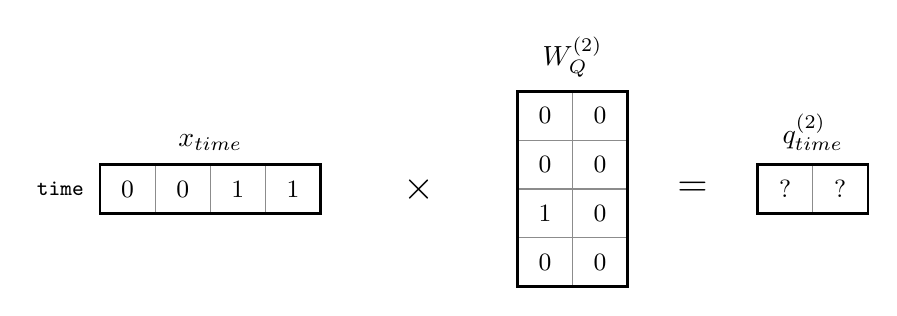
\begin{tikzpicture}
\draw[black!45, fill=white] (0.810,0.310) rectangle (1.510,-0.310);
\node[font=\small, text=black] at (1.160,0.000) {$0$};
\draw[black!45, fill=white] (1.510,0.310) rectangle (2.210,-0.310);
\node[font=\small, text=black] at (1.860,0.000) {$0$};
\draw[black!45, fill=white] (2.210,0.310) rectangle (2.910,-0.310);
\node[font=\small, text=black] at (2.560,0.000) {$1$};
\draw[black!45, fill=white] (2.910,0.310) rectangle (3.610,-0.310);
\node[font=\small, text=black] at (3.260,0.000) {$1$};
\draw[line width=0.9pt] (0.810,0.310) rectangle (3.610,-0.310);
\node[anchor=east, font=\footnotesize\ttfamily] at (0.730,0.000) {time};
\node[anchor=south, font=\normalsize] at (2.210,0.360) {$\bm x_{\text{time}}$};
\node[font=\Large] at (4.860,0) {$\times$};
\draw[black!45, fill=white] (6.110,1.240) rectangle (6.810,0.620);
\node[font=\small, text=black] at (6.460,0.930) {$0$};
\draw[black!45, fill=white] (6.810,1.240) rectangle (7.510,0.620);
\node[font=\small, text=black] at (7.160,0.930) {$0$};
\draw[black!45, fill=white] (6.110,0.620) rectangle (6.810,0.000);
\node[font=\small, text=black] at (6.460,0.310) {$0$};
\draw[black!45, fill=white] (6.810,0.620) rectangle (7.510,0.000);
\node[font=\small, text=black] at (7.160,0.310) {$0$};
\draw[black!45, fill=white] (6.110,0.000) rectangle (6.810,-0.620);
\node[font=\small, text=black] at (6.460,-0.310) {$1$};
\draw[black!45, fill=white] (6.810,0.000) rectangle (7.510,-0.620);
\node[font=\small, text=black] at (7.160,-0.310) {$0$};
\draw[black!45, fill=white] (6.110,-0.620) rectangle (6.810,-1.240);
\node[font=\small, text=black] at (6.460,-0.930) {$0$};
\draw[black!45, fill=white] (6.810,-0.620) rectangle (7.510,-1.240);
\node[font=\small, text=black] at (7.160,-0.930) {$0$};
\draw[line width=0.9pt] (6.110,1.240) rectangle (7.510,-1.240);
\node[anchor=south, font=\normalsize] at (6.810,1.290) {$W_Q^{(2)}$};
\node[font=\Large] at (8.335,0) {$=$};
\draw[black!45, fill=white] (9.160,0.310) rectangle (9.860,-0.310);
\node[font=\small, text=black] at (9.510,0.000) {?};
\draw[black!45, fill=white] (9.860,0.310) rectangle (10.560,-0.310);
\node[font=\small, text=black] at (10.210,0.000) {?};
\draw[line width=0.9pt] (9.160,0.310) rectangle (10.560,-0.310);
\node[anchor=south, font=\normalsize] at (9.860,0.360) {$\bm q^{(2)}_{\text{time}}$};
\end{tikzpicture}
\\[10pt]
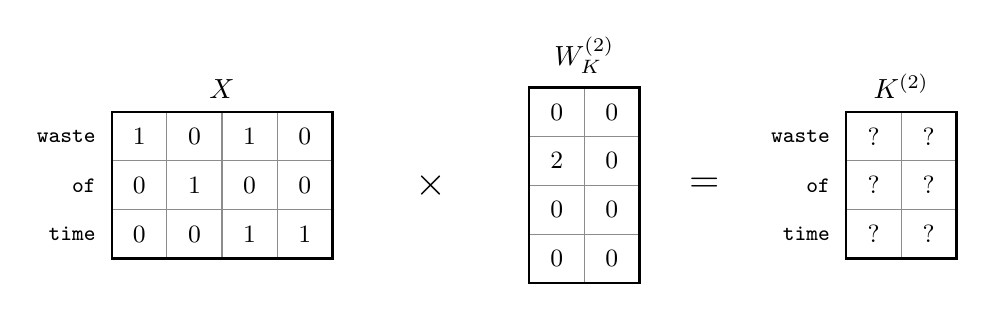
\begin{tikzpicture}
\draw[black!45, fill=white] (0.975,0.930) rectangle (1.675,0.310);
\node[font=\small, text=black] at (1.325,0.620) {$1$};
\draw[black!45, fill=white] (1.675,0.930) rectangle (2.375,0.310);
\node[font=\small, text=black] at (2.025,0.620) {$0$};
\draw[black!45, fill=white] (2.375,0.930) rectangle (3.075,0.310);
\node[font=\small, text=black] at (2.725,0.620) {$1$};
\draw[black!45, fill=white] (3.075,0.930) rectangle (3.775,0.310);
\node[font=\small, text=black] at (3.425,0.620) {$0$};
\draw[black!45, fill=white] (0.975,0.310) rectangle (1.675,-0.310);
\node[font=\small, text=black] at (1.325,-0.000) {$0$};
\draw[black!45, fill=white] (1.675,0.310) rectangle (2.375,-0.310);
\node[font=\small, text=black] at (2.025,-0.000) {$1$};
\draw[black!45, fill=white] (2.375,0.310) rectangle (3.075,-0.310);
\node[font=\small, text=black] at (2.725,-0.000) {$0$};
\draw[black!45, fill=white] (3.075,0.310) rectangle (3.775,-0.310);
\node[font=\small, text=black] at (3.425,-0.000) {$0$};
\draw[black!45, fill=white] (0.975,-0.310) rectangle (1.675,-0.930);
\node[font=\small, text=black] at (1.325,-0.620) {$0$};
\draw[black!45, fill=white] (1.675,-0.310) rectangle (2.375,-0.930);
\node[font=\small, text=black] at (2.025,-0.620) {$0$};
\draw[black!45, fill=white] (2.375,-0.310) rectangle (3.075,-0.930);
\node[font=\small, text=black] at (2.725,-0.620) {$1$};
\draw[black!45, fill=white] (3.075,-0.310) rectangle (3.775,-0.930);
\node[font=\small, text=black] at (3.425,-0.620) {$1$};
\draw[line width=0.9pt] (0.975,0.930) rectangle (3.775,-0.930);
\node[anchor=east, font=\footnotesize\ttfamily] at (0.895,0.620) {waste};
\node[anchor=east, font=\footnotesize\ttfamily] at (0.895,-0.000) {of};
\node[anchor=east, font=\footnotesize\ttfamily] at (0.895,-0.620) {time};
\node[anchor=south, font=\normalsize] at (2.375,0.980) {$X$};
\node[font=\Large] at (5.025,0) {$\times$};
\draw[black!45, fill=white] (6.275,1.240) rectangle (6.975,0.620);
\node[font=\small, text=black] at (6.625,0.930) {$0$};
\draw[black!45, fill=white] (6.975,1.240) rectangle (7.675,0.620);
\node[font=\small, text=black] at (7.325,0.930) {$0$};
\draw[black!45, fill=white] (6.275,0.620) rectangle (6.975,0.000);
\node[font=\small, text=black] at (6.625,0.310) {$2$};
\draw[black!45, fill=white] (6.975,0.620) rectangle (7.675,0.000);
\node[font=\small, text=black] at (7.325,0.310) {$0$};
\draw[black!45, fill=white] (6.275,0.000) rectangle (6.975,-0.620);
\node[font=\small, text=black] at (6.625,-0.310) {$0$};
\draw[black!45, fill=white] (6.975,0.000) rectangle (7.675,-0.620);
\node[font=\small, text=black] at (7.325,-0.310) {$0$};
\draw[black!45, fill=white] (6.275,-0.620) rectangle (6.975,-1.240);
\node[font=\small, text=black] at (6.625,-0.930) {$0$};
\draw[black!45, fill=white] (6.975,-0.620) rectangle (7.675,-1.240);
\node[font=\small, text=black] at (7.325,-0.930) {$0$};
\draw[line width=0.9pt] (6.275,1.240) rectangle (7.675,-1.240);
\node[anchor=south, font=\normalsize] at (6.975,1.290) {$W_K^{(2)}$};
\node[font=\Large] at (8.500,0) {$=$};
\draw[black!45, fill=white] (10.300,0.930) rectangle (11.000,0.310);
\node[font=\small, text=black] at (10.650,0.620) {?};
\draw[black!45, fill=white] (11.000,0.930) rectangle (11.700,0.310);
\node[font=\small, text=black] at (11.350,0.620) {?};
\draw[black!45, fill=white] (10.300,0.310) rectangle (11.000,-0.310);
\node[font=\small, text=black] at (10.650,-0.000) {?};
\draw[black!45, fill=white] (11.000,0.310) rectangle (11.700,-0.310);
\node[font=\small, text=black] at (11.350,-0.000) {?};
\draw[black!45, fill=white] (10.300,-0.310) rectangle (11.000,-0.930);
\node[font=\small, text=black] at (10.650,-0.620) {?};
\draw[black!45, fill=white] (11.000,-0.310) rectangle (11.700,-0.930);
\node[font=\small, text=black] at (11.350,-0.620) {?};
\draw[line width=0.9pt] (10.300,0.930) rectangle (11.700,-0.930);
\node[anchor=east, font=\footnotesize\ttfamily] at (10.220,0.620) {waste};
\node[anchor=east, font=\footnotesize\ttfamily] at (10.220,-0.000) {of};
\node[anchor=east, font=\footnotesize\ttfamily] at (10.220,-0.620) {time};
\node[anchor=south, font=\normalsize] at (11.000,0.980) {$K^{(2)}$};
\end{tikzpicture}
}
\captionof{figure}{Head 2, your turn. Multiply as in Figure~\ref{fig:ch5headone} and fill in the cells marked ?.}
\label{fig:ch5headtwo}
\end{center}


\Sanity The scaled scores are
\[\nFiveStwoScaled,\]
and the shares come out as $(\nFiveAtwoWaste,\ \nFiveAtwoOf,\ \nFiveAtwoTime)$: \nFivePtwoOf\% on \tok{of}. The shares add to 1, and the
favourite is the token you predicted.

\begin{center}
\small
\begin{tabular}{@{}l c c c@{}}
\toprule
\tok{time} attends to & \tok{waste} & \tok{of} & \tok{time}\\
\midrule
Chapter 3 (one head, $d_k=4$) & \nFiveChThreeWaste\% & \nFiveChThreeOf\% & \apctTime\%\\
Head 1 ($d_k=2$) & \nFivePoneWaste\% & \nFivePoneOf\% & \nFivePoneTime\%\\
Head 2 ($d_k=2$) & \nFivePtwoWaste\% & \nFivePtwoOf\% & \nFivePtwoTime\%\\
\bottomrule
\end{tabular}
\end{center}

Each head now spends its whole budget on its own question. One head mostly hears \tok{waste}; the other mostly
hears \tok{of}.

\begin{breaks}
Our two reporters have tidy, nameable briefs because we wrote the weights by hand. Heads in trained models
are learned, often overlap, and many have no neat job. Michel, Levy and Neubig (2019) removed most of the heads
of trained models one at a time and found that many could go with little loss.
\end{breaks}

\Why Splitting the width keeps the cost the same (the four machines of the block still hold $4\times d^2$
numbers in total) while giving the token several independent budgets of attention. The price is that each head
asks with fewer numbers, so each question is cruder.

\begin{wrongidea}{5.1}
\emph{More heads is always better.} With the width fixed, more heads means narrower heads. Taken to the
extreme, a head with $d_k=1$ compares single numbers, a very blunt question. The number of heads is a trade-off to choose, and Chapter 11
treats it as one.
\end{wrongidea}

\begin{wrongidea}{5.5}
\emph{Each head has a fixed job, like ``the grammar head''.} Our toy heads do, because we designed them. In a
trained model a head's job is whatever helped predict the next token, and it is often a mixture.
\end{wrongidea}

\begin{checkq}
A model has width $d=64$. You change it from 2 heads to 8 heads and keep $d$ fixed. What happens?
\begin{options}
\item Each head becomes 4 times wider, so each question is sharper.
\item Each head drops from 32 to 8 numbers, and there are 4 times as many independent sets of shares.
\item The number of attention weights grows 4 times.
\item The model necessarily gets better, because more heads see more.
\end{options}
\end{checkq}

\Summary{Splitting the width into heads gives a token several separate attention budgets at no extra cost,
each one asking a cruder question.}

%---------------------------------------------------------------------
\subsection*{5.3\quad Stitching the notes together}

\Picture The two reporters staple their notes side by side, and an editor rewrites the stapled page in the
house style.

\Exactly Each head hands back a short arrow for \tok{time}, of width $d_k=2$. Concatenate them into one
arrow of width $d=4$, then multiply by an output matrix $W_O$ ($d\times d$), the editor:
\[
\bm{o}_{\text{time}} = \big[\,\bm{o}^{(1)}_{\text{time}}\ \ \bm{o}^{(2)}_{\text{time}}\,\big]\,W_O \shape{(1\times d)(d\times d)=1\times d}
\]
Figure~\ref{fig:ch5concat} shows both steps with the numbers.

\begin{center}
\fitwidthFourFive{% AUTO-GENERATED by code/figlib.py helpers -- do not edit
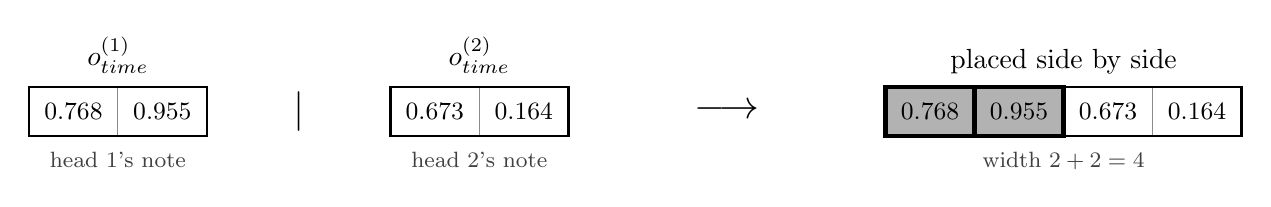
\begin{tikzpicture}
\draw[black!45, fill=white] (0.000,0.310) rectangle (1.130,-0.310);
\node[font=\small, text=black] at (0.565,0.000) {$0.768$};
\draw[black!45, fill=white] (1.130,0.310) rectangle (2.260,-0.310);
\node[font=\small, text=black] at (1.695,0.000) {$0.955$};
\draw[line width=0.9pt] (0.000,0.310) rectangle (2.260,-0.310);
\node[anchor=south, font=\normalsize] at (1.130,0.360) {$\bm o^{(1)}_{\text{time}}$};
\node[anchor=north, font=\footnotesize, text=black!75] at (1.130,-0.390) {head 1's note};
\node[font=\Large] at (3.425,0) {$\big|$};
\draw[black!45, fill=white] (4.590,0.310) rectangle (5.720,-0.310);
\node[font=\small, text=black] at (5.155,0.000) {$0.673$};
\draw[black!45, fill=white] (5.720,0.310) rectangle (6.850,-0.310);
\node[font=\small, text=black] at (6.285,0.000) {$0.164$};
\draw[line width=0.9pt] (4.590,0.310) rectangle (6.850,-0.310);
\node[anchor=south, font=\normalsize] at (5.720,0.360) {$\bm o^{(2)}_{\text{time}}$};
\node[anchor=north, font=\footnotesize, text=black!75] at (5.720,-0.390) {head 2's note};
\node[font=\Large] at (8.865,0) {$\longrightarrow$};
\draw[black!45, fill=black!30] (10.880,0.310) rectangle (12.010,-0.310);
\node[font=\small, text=black] at (11.445,0.000) {$0.768$};
\draw[black!45, fill=black!30] (12.010,0.310) rectangle (13.140,-0.310);
\node[font=\small, text=black] at (12.575,0.000) {$0.955$};
\draw[black!45, fill=white] (13.140,0.310) rectangle (14.270,-0.310);
\node[font=\small, text=black] at (13.705,0.000) {$0.673$};
\draw[black!45, fill=white] (14.270,0.310) rectangle (15.400,-0.310);
\node[font=\small, text=black] at (14.835,0.000) {$0.164$};
\draw[line width=1.6pt] (10.880,0.310) rectangle (12.010,-0.310);
\draw[line width=1.6pt] (12.010,0.310) rectangle (13.140,-0.310);
\draw[line width=0.9pt] (10.880,0.310) rectangle (15.400,-0.310);
\node[anchor=south, font=\normalsize] at (13.140,0.360) {placed side by side};
\node[anchor=north, font=\footnotesize, text=black!75] at (13.140,-0.390) {width $2+2=4$};
\end{tikzpicture}
\\[10pt]
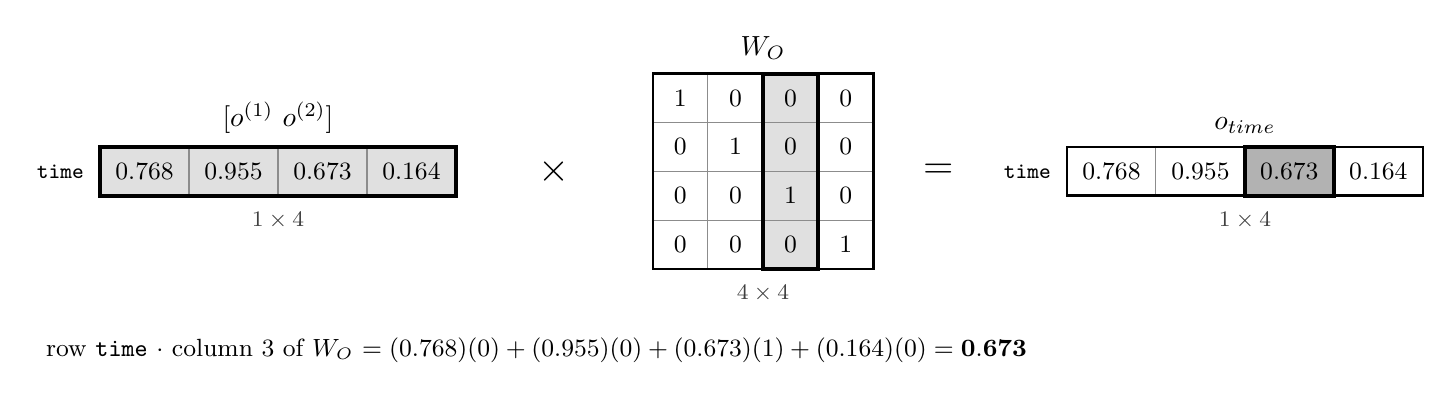
\begin{tikzpicture}
\draw[black!45, fill=black!12] (0.810,0.310) rectangle (1.940,-0.310);
\node[font=\small, text=black] at (1.375,0.000) {$0.768$};
\draw[black!45, fill=black!12] (1.940,0.310) rectangle (3.070,-0.310);
\node[font=\small, text=black] at (2.505,0.000) {$0.955$};
\draw[black!45, fill=black!12] (3.070,0.310) rectangle (4.200,-0.310);
\node[font=\small, text=black] at (3.635,0.000) {$0.673$};
\draw[black!45, fill=black!12] (4.200,0.310) rectangle (5.330,-0.310);
\node[font=\small, text=black] at (4.765,0.000) {$0.164$};
\draw[line width=1.4pt] (0.810,0.310) rectangle (5.330,-0.310);
\draw[line width=0.9pt] (0.810,0.310) rectangle (5.330,-0.310);
\node[anchor=east, font=\footnotesize\ttfamily] at (0.730,0.000) {time};
\node[anchor=south, font=\normalsize] at (3.070,0.360) {$[\bm o^{(1)}\ \bm o^{(2)}]$};
\node[anchor=north, font=\footnotesize, text=black!75] at (3.070,-0.390) {$1\times4$};
\node[font=\Large] at (6.580,0) {$\times$};
\draw[black!45, fill=white] (7.830,1.240) rectangle (8.530,0.620);
\node[font=\small, text=black] at (8.180,0.930) {$1$};
\draw[black!45, fill=white] (8.530,1.240) rectangle (9.230,0.620);
\node[font=\small, text=black] at (8.880,0.930) {$0$};
\draw[black!45, fill=black!12] (9.230,1.240) rectangle (9.930,0.620);
\node[font=\small, text=black] at (9.580,0.930) {$0$};
\draw[black!45, fill=white] (9.930,1.240) rectangle (10.630,0.620);
\node[font=\small, text=black] at (10.280,0.930) {$0$};
\draw[black!45, fill=white] (7.830,0.620) rectangle (8.530,0.000);
\node[font=\small, text=black] at (8.180,0.310) {$0$};
\draw[black!45, fill=white] (8.530,0.620) rectangle (9.230,0.000);
\node[font=\small, text=black] at (8.880,0.310) {$1$};
\draw[black!45, fill=black!12] (9.230,0.620) rectangle (9.930,0.000);
\node[font=\small, text=black] at (9.580,0.310) {$0$};
\draw[black!45, fill=white] (9.930,0.620) rectangle (10.630,0.000);
\node[font=\small, text=black] at (10.280,0.310) {$0$};
\draw[black!45, fill=white] (7.830,0.000) rectangle (8.530,-0.620);
\node[font=\small, text=black] at (8.180,-0.310) {$0$};
\draw[black!45, fill=white] (8.530,0.000) rectangle (9.230,-0.620);
\node[font=\small, text=black] at (8.880,-0.310) {$0$};
\draw[black!45, fill=black!12] (9.230,0.000) rectangle (9.930,-0.620);
\node[font=\small, text=black] at (9.580,-0.310) {$1$};
\draw[black!45, fill=white] (9.930,0.000) rectangle (10.630,-0.620);
\node[font=\small, text=black] at (10.280,-0.310) {$0$};
\draw[black!45, fill=white] (7.830,-0.620) rectangle (8.530,-1.240);
\node[font=\small, text=black] at (8.180,-0.930) {$0$};
\draw[black!45, fill=white] (8.530,-0.620) rectangle (9.230,-1.240);
\node[font=\small, text=black] at (8.880,-0.930) {$0$};
\draw[black!45, fill=black!12] (9.230,-0.620) rectangle (9.930,-1.240);
\node[font=\small, text=black] at (9.580,-0.930) {$0$};
\draw[black!45, fill=white] (9.930,-0.620) rectangle (10.630,-1.240);
\node[font=\small, text=black] at (10.280,-0.930) {$1$};
\draw[line width=1.4pt] (9.230,1.240) rectangle (9.930,-1.240);
\draw[line width=0.9pt] (7.830,1.240) rectangle (10.630,-1.240);
\node[anchor=south, font=\normalsize] at (9.230,1.290) {$W_O$};
\node[anchor=north, font=\footnotesize, text=black!75] at (9.230,-1.320) {$4\times4$};
\node[font=\Large] at (11.455,0) {$=$};
\draw[black!45, fill=white] (13.090,0.310) rectangle (14.220,-0.310);
\node[font=\small, text=black] at (13.655,0.000) {$0.768$};
\draw[black!45, fill=white] (14.220,0.310) rectangle (15.350,-0.310);
\node[font=\small, text=black] at (14.785,0.000) {$0.955$};
\draw[black!45, fill=black!30] (15.350,0.310) rectangle (16.480,-0.310);
\node[font=\small, text=black] at (15.915,0.000) {$0.673$};
\draw[black!45, fill=white] (16.480,0.310) rectangle (17.610,-0.310);
\node[font=\small, text=black] at (17.045,0.000) {$0.164$};
\draw[line width=1.6pt] (15.350,0.310) rectangle (16.480,-0.310);
\draw[line width=0.9pt] (13.090,0.310) rectangle (17.610,-0.310);
\node[anchor=east, font=\footnotesize\ttfamily] at (13.010,0.000) {time};
\node[anchor=south, font=\normalsize] at (15.350,0.360) {$\bm o_{\text{time}}$};
\node[anchor=north, font=\footnotesize, text=black!75] at (15.350,-0.390) {$1\times4$};
\node[anchor=north west, font=\small, align=left] at (0,-1.990) {row \texttt{time} $\cdot$ column 3 of $W_O$ $= (0.768)(0) + (0.955)(0) + (0.673)(1) + (0.164)(0) = \mathbf{0.673}$};
\end{tikzpicture}
}
\captionof{figure}{Stitching the heads. Top: head 1's note and head 2's note are placed side by side (head 1's part shaded). Bottom: the stitched arrow times $W_O$. Our toy $W_O$ is the identity, so each cell passes straight through; a trained $W_O$ would mix them.}
\label{fig:ch5concat}
\end{center}

In the toy we set $W_O$ to the identity matrix, so you can see head 1's note in the first two numbers and head
2's in the last two. A trained $W_O$ mixes them, so that what one head found can be combined with what the other
found.

\Why Concatenation keeps the heads' answers apart, which was the point of \S5.1. $W_O$ then brings them back
into the shared $d$-dimensional space every later step uses.

\Summary{Head outputs are placed side by side and mixed back to width $d$ by one learned matrix.}

%---------------------------------------------------------------------
\subsection*{5.4\quad The MLP: each token thinks alone}

After attention, \tok{time} has heard from \tok{waste} and \tok{of}. What does it do with what it heard?

\Predict Before reading on, tell me: should this next step look at the other tokens again, or work on each
token alone? Why?

\Picture After a meeting, each person goes back to their own desk with their notes and checks them against a
personal list of patterns: ``if I see this, then write that''. Nobody talks during this part.

\Exactly The MLP (multi-layer perceptron, also called the feed-forward network) applies to every token's
arrow separately:
\[
\operatorname{MLP}(\bm{h}) = \max(0,\ \bm{h}W_1 + \bm{b}_1)\,W_2
\shape{(1\times d)(d\times d_{\text{ff}})(d_{\text{ff}}\times d)=1\times d}
\]
Read it as a list of $d_{\text{ff}}$ patterns. Column $j$ of $W_1$ is a \emph{key}: a direction to check for.
The dot product of $\bm{h}$ with it, plus a threshold $b_j$, says how strongly the pattern is present. The
function $\max(0,\cdot)$, called ReLU, lets a pattern \emph{fire} only above its threshold. Row $j$ of $W_2$ is
the matching \emph{value}: what to write when the pattern fires. Geva and colleagues (2021) showed that trained
MLPs behave very much like this key--value memory.

Our toy has $d_{\text{ff}}=\nFiveDff$, four times $d$, as in the original transformer and GPT-2. To keep the
arithmetic on paper, only three neurons are switched on; the other thirteen are all zeros.

\begin{center}
\small
\begin{tabular}{@{}l l c l@{}}
\toprule
neuron & key (column of $W_1$) & threshold & value (row of $W_2$)\\
\midrule
1 & $\nFiveKeyOne$ & $\nFiveBiasOne$ & $\nFiveValOne$\\
2 & $\nFiveKeyTwo$ & $\nFiveBiasTwo$ & $\nFiveValTwo$\\
3 & $\nFiveKeyThree$ & $\nFiveBiasThree$ & $\nFiveValThree$\\
\bottomrule
\end{tabular}
\end{center}

The MLP reads $\bm{h}_1$, the token's arrow after attention has been added in (\S5.5 explains the adding).
For our three tokens it is
\[
H_1 = \begin{array}{r}\tok{waste}\\ \tok{of}\\ \tok{time}\end{array}\!\!\nFiveHone .
\]
Now follow the three steps of the formula in pictures. First, every row of $H_1$ is checked against every
key (Figure~\ref{fig:ch5mlpone}).

\begin{center}
\fitwidthFourFive{% AUTO-GENERATED by code/figlib.py helpers -- do not edit
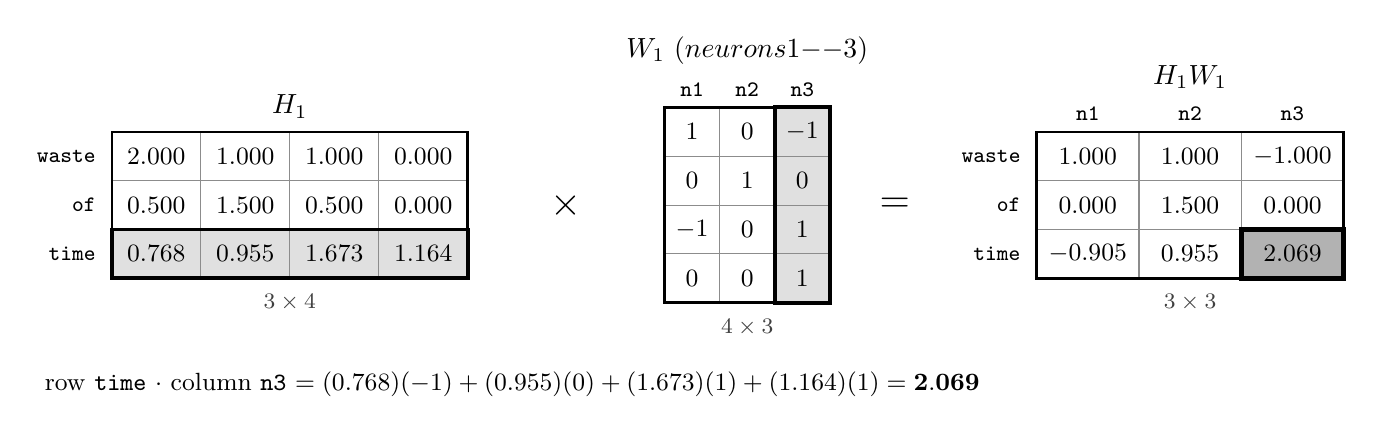
\begin{tikzpicture}
\draw[black!45, fill=white] (0.975,0.930) rectangle (2.105,0.310);
\node[font=\small, text=black] at (1.540,0.620) {$2.000$};
\draw[black!45, fill=white] (2.105,0.930) rectangle (3.235,0.310);
\node[font=\small, text=black] at (2.670,0.620) {$1.000$};
\draw[black!45, fill=white] (3.235,0.930) rectangle (4.365,0.310);
\node[font=\small, text=black] at (3.800,0.620) {$1.000$};
\draw[black!45, fill=white] (4.365,0.930) rectangle (5.495,0.310);
\node[font=\small, text=black] at (4.930,0.620) {$0.000$};
\draw[black!45, fill=white] (0.975,0.310) rectangle (2.105,-0.310);
\node[font=\small, text=black] at (1.540,-0.000) {$0.500$};
\draw[black!45, fill=white] (2.105,0.310) rectangle (3.235,-0.310);
\node[font=\small, text=black] at (2.670,-0.000) {$1.500$};
\draw[black!45, fill=white] (3.235,0.310) rectangle (4.365,-0.310);
\node[font=\small, text=black] at (3.800,-0.000) {$0.500$};
\draw[black!45, fill=white] (4.365,0.310) rectangle (5.495,-0.310);
\node[font=\small, text=black] at (4.930,-0.000) {$0.000$};
\draw[black!45, fill=black!12] (0.975,-0.310) rectangle (2.105,-0.930);
\node[font=\small, text=black] at (1.540,-0.620) {$0.768$};
\draw[black!45, fill=black!12] (2.105,-0.310) rectangle (3.235,-0.930);
\node[font=\small, text=black] at (2.670,-0.620) {$0.955$};
\draw[black!45, fill=black!12] (3.235,-0.310) rectangle (4.365,-0.930);
\node[font=\small, text=black] at (3.800,-0.620) {$1.673$};
\draw[black!45, fill=black!12] (4.365,-0.310) rectangle (5.495,-0.930);
\node[font=\small, text=black] at (4.930,-0.620) {$1.164$};
\draw[line width=1.4pt] (0.975,-0.310) rectangle (5.495,-0.930);
\draw[line width=0.9pt] (0.975,0.930) rectangle (5.495,-0.930);
\node[anchor=east, font=\footnotesize\ttfamily] at (0.895,0.620) {waste};
\node[anchor=east, font=\footnotesize\ttfamily] at (0.895,-0.000) {of};
\node[anchor=east, font=\footnotesize\ttfamily] at (0.895,-0.620) {time};
\node[anchor=south, font=\normalsize] at (3.235,0.980) {$H_1$};
\node[anchor=north, font=\footnotesize, text=black!75] at (3.235,-1.010) {$3\times4$};
\node[font=\Large] at (6.745,0) {$\times$};
\draw[black!45, fill=white] (7.995,1.240) rectangle (8.695,0.620);
\node[font=\small, text=black] at (8.345,0.930) {$1$};
\draw[black!45, fill=white] (8.695,1.240) rectangle (9.395,0.620);
\node[font=\small, text=black] at (9.045,0.930) {$0$};
\draw[black!45, fill=black!12] (9.395,1.240) rectangle (10.095,0.620);
\node[font=\small, text=black] at (9.745,0.930) {$-1$};
\draw[black!45, fill=white] (7.995,0.620) rectangle (8.695,0.000);
\node[font=\small, text=black] at (8.345,0.310) {$0$};
\draw[black!45, fill=white] (8.695,0.620) rectangle (9.395,0.000);
\node[font=\small, text=black] at (9.045,0.310) {$1$};
\draw[black!45, fill=black!12] (9.395,0.620) rectangle (10.095,0.000);
\node[font=\small, text=black] at (9.745,0.310) {$0$};
\draw[black!45, fill=white] (7.995,0.000) rectangle (8.695,-0.620);
\node[font=\small, text=black] at (8.345,-0.310) {$-1$};
\draw[black!45, fill=white] (8.695,0.000) rectangle (9.395,-0.620);
\node[font=\small, text=black] at (9.045,-0.310) {$0$};
\draw[black!45, fill=black!12] (9.395,0.000) rectangle (10.095,-0.620);
\node[font=\small, text=black] at (9.745,-0.310) {$1$};
\draw[black!45, fill=white] (7.995,-0.620) rectangle (8.695,-1.240);
\node[font=\small, text=black] at (8.345,-0.930) {$0$};
\draw[black!45, fill=white] (8.695,-0.620) rectangle (9.395,-1.240);
\node[font=\small, text=black] at (9.045,-0.930) {$0$};
\draw[black!45, fill=black!12] (9.395,-0.620) rectangle (10.095,-1.240);
\node[font=\small, text=black] at (9.745,-0.930) {$1$};
\draw[line width=1.4pt] (9.395,1.240) rectangle (10.095,-1.240);
\draw[line width=0.9pt] (7.995,1.240) rectangle (10.095,-1.240);
\node[anchor=south, font=\footnotesize\ttfamily] at (8.345,1.260) {n1};
\node[anchor=south, font=\footnotesize\ttfamily] at (9.045,1.260) {n2};
\node[anchor=south, font=\footnotesize\ttfamily] at (9.745,1.260) {n3};
\node[anchor=south, font=\normalsize] at (9.045,1.660) {$W_1\ (\text{neurons }1\text{--}3)$};
\node[anchor=north, font=\footnotesize, text=black!75] at (9.045,-1.320) {$4\times3$};
\node[font=\Large] at (10.920,0) {$=$};
\draw[black!45, fill=white] (12.720,0.930) rectangle (14.020,0.310);
\node[font=\small, text=black] at (13.370,0.620) {$1.000$};
\draw[black!45, fill=white] (14.020,0.930) rectangle (15.320,0.310);
\node[font=\small, text=black] at (14.670,0.620) {$1.000$};
\draw[black!45, fill=white] (15.320,0.930) rectangle (16.620,0.310);
\node[font=\small, text=black] at (15.970,0.620) {$-1.000$};
\draw[black!45, fill=white] (12.720,0.310) rectangle (14.020,-0.310);
\node[font=\small, text=black] at (13.370,-0.000) {$0.000$};
\draw[black!45, fill=white] (14.020,0.310) rectangle (15.320,-0.310);
\node[font=\small, text=black] at (14.670,-0.000) {$1.500$};
\draw[black!45, fill=white] (15.320,0.310) rectangle (16.620,-0.310);
\node[font=\small, text=black] at (15.970,-0.000) {$0.000$};
\draw[black!45, fill=white] (12.720,-0.310) rectangle (14.020,-0.930);
\node[font=\small, text=black] at (13.370,-0.620) {$-0.905$};
\draw[black!45, fill=white] (14.020,-0.310) rectangle (15.320,-0.930);
\node[font=\small, text=black] at (14.670,-0.620) {$0.955$};
\draw[black!45, fill=black!30] (15.320,-0.310) rectangle (16.620,-0.930);
\node[font=\small, text=black] at (15.970,-0.620) {$2.069$};
\draw[line width=1.6pt] (15.320,-0.310) rectangle (16.620,-0.930);
\draw[line width=0.9pt] (12.720,0.930) rectangle (16.620,-0.930);
\node[anchor=east, font=\footnotesize\ttfamily] at (12.640,0.620) {waste};
\node[anchor=east, font=\footnotesize\ttfamily] at (12.640,-0.000) {of};
\node[anchor=east, font=\footnotesize\ttfamily] at (12.640,-0.620) {time};
\node[anchor=south, font=\footnotesize\ttfamily] at (13.370,0.950) {n1};
\node[anchor=south, font=\footnotesize\ttfamily] at (14.670,0.950) {n2};
\node[anchor=south, font=\footnotesize\ttfamily] at (15.970,0.950) {n3};
\node[anchor=south, font=\normalsize] at (14.670,1.350) {$H_1W_1$};
\node[anchor=north, font=\footnotesize, text=black!75] at (14.670,-1.010) {$3\times3$};
\node[anchor=north west, font=\small, align=left] at (0,-1.990) {row \texttt{time} $\cdot$ column \texttt{n3} $= (0.768)(-1) + (0.955)(0) + (1.673)(1) + (1.164)(1) = \mathbf{2.069}$};
\end{tikzpicture}
}
\captionof{figure}{Step 1, the checks. Each column of $W_1$ is one neuron's key. The outlined row of $H_1$ (\tok{time}) meets neuron 3's key and gives the dark cell. Only the three neurons that are switched on are drawn; the other thirteen columns are zeros.}
\label{fig:ch5mlpone}
\end{center}

Second, add each neuron's threshold and let ReLU switch off everything negative
(Figure~\ref{fig:ch5mlptwo}).

\begin{center}
\fitwidthFourFive{% AUTO-GENERATED by code/figlib.py helpers -- do not edit
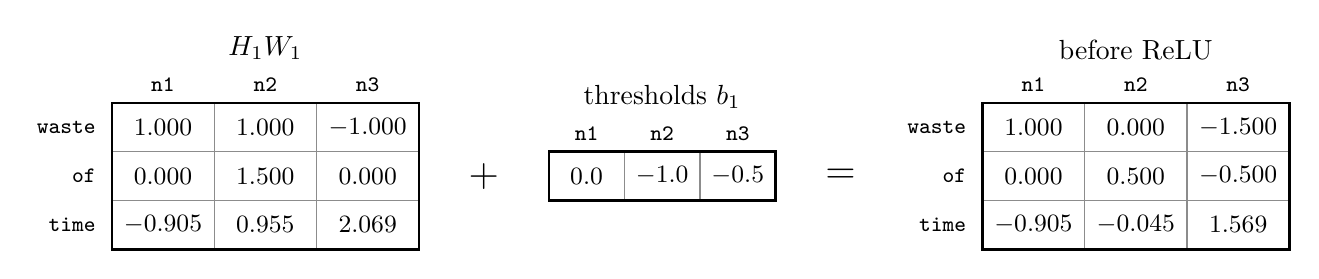
\begin{tikzpicture}
\draw[black!45, fill=white] (0.975,0.930) rectangle (2.275,0.310);
\node[font=\small, text=black] at (1.625,0.620) {$1.000$};
\draw[black!45, fill=white] (2.275,0.930) rectangle (3.575,0.310);
\node[font=\small, text=black] at (2.925,0.620) {$1.000$};
\draw[black!45, fill=white] (3.575,0.930) rectangle (4.875,0.310);
\node[font=\small, text=black] at (4.225,0.620) {$-1.000$};
\draw[black!45, fill=white] (0.975,0.310) rectangle (2.275,-0.310);
\node[font=\small, text=black] at (1.625,-0.000) {$0.000$};
\draw[black!45, fill=white] (2.275,0.310) rectangle (3.575,-0.310);
\node[font=\small, text=black] at (2.925,-0.000) {$1.500$};
\draw[black!45, fill=white] (3.575,0.310) rectangle (4.875,-0.310);
\node[font=\small, text=black] at (4.225,-0.000) {$0.000$};
\draw[black!45, fill=white] (0.975,-0.310) rectangle (2.275,-0.930);
\node[font=\small, text=black] at (1.625,-0.620) {$-0.905$};
\draw[black!45, fill=white] (2.275,-0.310) rectangle (3.575,-0.930);
\node[font=\small, text=black] at (2.925,-0.620) {$0.955$};
\draw[black!45, fill=white] (3.575,-0.310) rectangle (4.875,-0.930);
\node[font=\small, text=black] at (4.225,-0.620) {$2.069$};
\draw[line width=0.9pt] (0.975,0.930) rectangle (4.875,-0.930);
\node[anchor=east, font=\footnotesize\ttfamily] at (0.895,0.620) {waste};
\node[anchor=east, font=\footnotesize\ttfamily] at (0.895,-0.000) {of};
\node[anchor=east, font=\footnotesize\ttfamily] at (0.895,-0.620) {time};
\node[anchor=south, font=\footnotesize\ttfamily] at (1.625,0.950) {n1};
\node[anchor=south, font=\footnotesize\ttfamily] at (2.925,0.950) {n2};
\node[anchor=south, font=\footnotesize\ttfamily] at (4.225,0.950) {n3};
\node[anchor=south, font=\normalsize] at (2.925,1.350) {$H_1W_1$};
\node[font=\Large] at (5.700,0) {$+$};
\draw[black!45, fill=white] (6.525,0.310) rectangle (7.485,-0.310);
\node[font=\small, text=black] at (7.005,0.000) {$0.0$};
\draw[black!45, fill=white] (7.485,0.310) rectangle (8.445,-0.310);
\node[font=\small, text=black] at (7.965,0.000) {$-1.0$};
\draw[black!45, fill=white] (8.445,0.310) rectangle (9.405,-0.310);
\node[font=\small, text=black] at (8.925,0.000) {$-0.5$};
\draw[line width=0.9pt] (6.525,0.310) rectangle (9.405,-0.310);
\node[anchor=south, font=\footnotesize\ttfamily] at (7.005,0.330) {n1};
\node[anchor=south, font=\footnotesize\ttfamily] at (7.965,0.330) {n2};
\node[anchor=south, font=\footnotesize\ttfamily] at (8.925,0.330) {n3};
\node[anchor=south, font=\normalsize] at (7.965,0.730) {thresholds $\bm b_1$};
\node[font=\Large] at (10.230,0) {$=$};
\draw[black!45, fill=white] (12.030,0.930) rectangle (13.330,0.310);
\node[font=\small, text=black] at (12.680,0.620) {$1.000$};
\draw[black!45, fill=white] (13.330,0.930) rectangle (14.630,0.310);
\node[font=\small, text=black] at (13.980,0.620) {$0.000$};
\draw[black!45, fill=white] (14.630,0.930) rectangle (15.930,0.310);
\node[font=\small, text=black] at (15.280,0.620) {$-1.500$};
\draw[black!45, fill=white] (12.030,0.310) rectangle (13.330,-0.310);
\node[font=\small, text=black] at (12.680,-0.000) {$0.000$};
\draw[black!45, fill=white] (13.330,0.310) rectangle (14.630,-0.310);
\node[font=\small, text=black] at (13.980,-0.000) {$0.500$};
\draw[black!45, fill=white] (14.630,0.310) rectangle (15.930,-0.310);
\node[font=\small, text=black] at (15.280,-0.000) {$-0.500$};
\draw[black!45, fill=white] (12.030,-0.310) rectangle (13.330,-0.930);
\node[font=\small, text=black] at (12.680,-0.620) {$-0.905$};
\draw[black!45, fill=white] (13.330,-0.310) rectangle (14.630,-0.930);
\node[font=\small, text=black] at (13.980,-0.620) {$-0.045$};
\draw[black!45, fill=white] (14.630,-0.310) rectangle (15.930,-0.930);
\node[font=\small, text=black] at (15.280,-0.620) {$1.569$};
\draw[line width=0.9pt] (12.030,0.930) rectangle (15.930,-0.930);
\node[anchor=east, font=\footnotesize\ttfamily] at (11.950,0.620) {waste};
\node[anchor=east, font=\footnotesize\ttfamily] at (11.950,-0.000) {of};
\node[anchor=east, font=\footnotesize\ttfamily] at (11.950,-0.620) {time};
\node[anchor=south, font=\footnotesize\ttfamily] at (12.680,0.950) {n1};
\node[anchor=south, font=\footnotesize\ttfamily] at (13.980,0.950) {n2};
\node[anchor=south, font=\footnotesize\ttfamily] at (15.280,0.950) {n3};
\node[anchor=south, font=\normalsize] at (13.980,1.350) {before ReLU};
\end{tikzpicture}
\\[10pt]
\begin{tikzpicture}
\draw[black!45, fill=white] (0.975,0.930) rectangle (2.275,0.310);
\node[font=\small, text=black] at (1.625,0.620) {$1.000$};
\draw[black!45, fill=white] (2.275,0.930) rectangle (3.575,0.310);
\node[font=\small, text=black] at (2.925,0.620) {$0.000$};
\draw[black!45, fill=white] (3.575,0.930) rectangle (4.875,0.310);
\node[font=\small, text=black] at (4.225,0.620) {$-1.500$};
\draw[black!45, fill=white] (0.975,0.310) rectangle (2.275,-0.310);
\node[font=\small, text=black] at (1.625,-0.000) {$0.000$};
\draw[black!45, fill=white] (2.275,0.310) rectangle (3.575,-0.310);
\node[font=\small, text=black] at (2.925,-0.000) {$0.500$};
\draw[black!45, fill=white] (3.575,0.310) rectangle (4.875,-0.310);
\node[font=\small, text=black] at (4.225,-0.000) {$-0.500$};
\draw[black!45, fill=white] (0.975,-0.310) rectangle (2.275,-0.930);
\node[font=\small, text=black] at (1.625,-0.620) {$-0.905$};
\draw[black!45, fill=white] (2.275,-0.310) rectangle (3.575,-0.930);
\node[font=\small, text=black] at (2.925,-0.620) {$-0.045$};
\draw[black!45, fill=white] (3.575,-0.310) rectangle (4.875,-0.930);
\node[font=\small, text=black] at (4.225,-0.620) {$1.569$};
\draw[line width=0.9pt] (0.975,0.930) rectangle (4.875,-0.930);
\node[anchor=east, font=\footnotesize\ttfamily] at (0.895,0.620) {waste};
\node[anchor=east, font=\footnotesize\ttfamily] at (0.895,-0.000) {of};
\node[anchor=east, font=\footnotesize\ttfamily] at (0.895,-0.620) {time};
\node[anchor=south, font=\footnotesize\ttfamily] at (1.625,0.950) {n1};
\node[anchor=south, font=\footnotesize\ttfamily] at (2.925,0.950) {n2};
\node[anchor=south, font=\footnotesize\ttfamily] at (4.225,0.950) {n3};
\node[anchor=south, font=\normalsize] at (2.925,1.350) {before ReLU};
\node[font=\Large] at (8.420,0) {$\xrightarrow{\ \max(0,\,\cdot)\ }$};
\draw[black!45, fill=black!30] (12.940,0.930) rectangle (14.070,0.310);
\node[font=\small, text=black] at (13.505,0.620) {$1.000$};
\draw[black!45, fill=white] (14.070,0.930) rectangle (15.200,0.310);
\node[font=\small, text=black] at (14.635,0.620) {$0.000$};
\draw[black!45, fill=white] (15.200,0.930) rectangle (16.330,0.310);
\node[font=\small, text=black] at (15.765,0.620) {$0.000$};
\draw[black!45, fill=white] (12.940,0.310) rectangle (14.070,-0.310);
\node[font=\small, text=black] at (13.505,-0.000) {$0.000$};
\draw[black!45, fill=black!30] (14.070,0.310) rectangle (15.200,-0.310);
\node[font=\small, text=black] at (14.635,-0.000) {$0.500$};
\draw[black!45, fill=white] (15.200,0.310) rectangle (16.330,-0.310);
\node[font=\small, text=black] at (15.765,-0.000) {$0.000$};
\draw[black!45, fill=white] (12.940,-0.310) rectangle (14.070,-0.930);
\node[font=\small, text=black] at (13.505,-0.620) {$0.000$};
\draw[black!45, fill=white] (14.070,-0.310) rectangle (15.200,-0.930);
\node[font=\small, text=black] at (14.635,-0.620) {$0.000$};
\draw[black!45, fill=black!30] (15.200,-0.310) rectangle (16.330,-0.930);
\node[font=\small, text=black] at (15.765,-0.620) {$1.569$};
\draw[line width=1.6pt] (12.940,0.930) rectangle (14.070,0.310);
\draw[line width=1.6pt] (14.070,0.310) rectangle (15.200,-0.310);
\draw[line width=1.6pt] (15.200,-0.310) rectangle (16.330,-0.930);
\draw[line width=0.9pt] (12.940,0.930) rectangle (16.330,-0.930);
\node[anchor=east, font=\footnotesize\ttfamily] at (12.860,0.620) {waste};
\node[anchor=east, font=\footnotesize\ttfamily] at (12.860,-0.000) {of};
\node[anchor=east, font=\footnotesize\ttfamily] at (12.860,-0.620) {time};
\node[anchor=south, font=\footnotesize\ttfamily] at (13.505,0.950) {n1};
\node[anchor=south, font=\footnotesize\ttfamily] at (14.635,0.950) {n2};
\node[anchor=south, font=\footnotesize\ttfamily] at (15.765,0.950) {n3};
\node[anchor=south, font=\normalsize] at (14.635,1.350) {after ReLU: negatives become 0};
\end{tikzpicture}
}
\captionof{figure}{Step 2, thresholds and ReLU. Top: the thresholds are added to every row. Bottom: every negative number becomes 0. What survives sits on the diagonal (dark cells): neuron 1 fires on \tok{waste}, neuron 2 on \tok{of}, neuron 3 on \tok{time}.}
\label{fig:ch5mlptwo}
\end{center}

Third, each firing neuron writes its value, scaled by how strongly it fired (Figure~\ref{fig:ch5mlpthree}).

\begin{center}
\fitwidthFourFive{% AUTO-GENERATED by code/figlib.py helpers -- do not edit
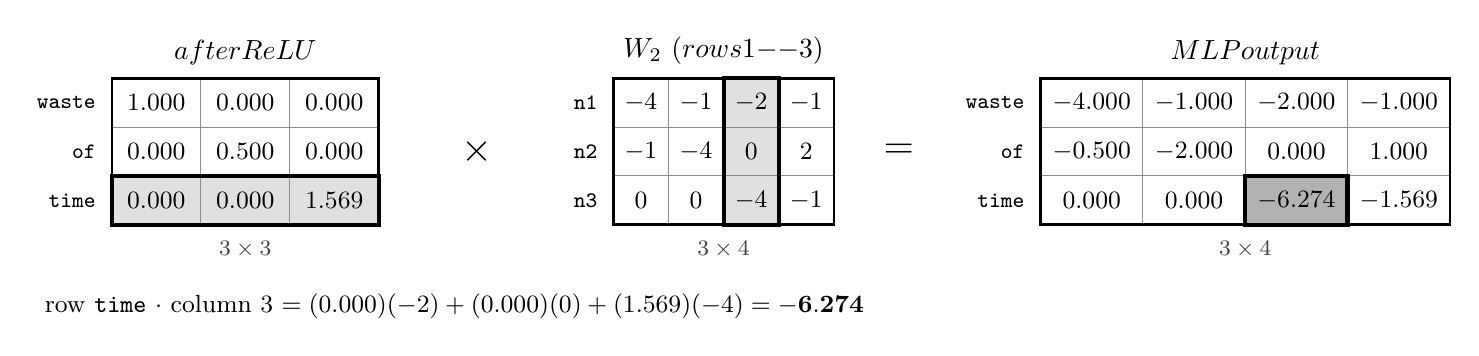
\begin{tikzpicture}
\draw[black!45, fill=white] (0.975,0.930) rectangle (2.105,0.310);
\node[font=\small, text=black] at (1.540,0.620) {$1.000$};
\draw[black!45, fill=white] (2.105,0.930) rectangle (3.235,0.310);
\node[font=\small, text=black] at (2.670,0.620) {$0.000$};
\draw[black!45, fill=white] (3.235,0.930) rectangle (4.365,0.310);
\node[font=\small, text=black] at (3.800,0.620) {$0.000$};
\draw[black!45, fill=white] (0.975,0.310) rectangle (2.105,-0.310);
\node[font=\small, text=black] at (1.540,-0.000) {$0.000$};
\draw[black!45, fill=white] (2.105,0.310) rectangle (3.235,-0.310);
\node[font=\small, text=black] at (2.670,-0.000) {$0.500$};
\draw[black!45, fill=white] (3.235,0.310) rectangle (4.365,-0.310);
\node[font=\small, text=black] at (3.800,-0.000) {$0.000$};
\draw[black!45, fill=black!12] (0.975,-0.310) rectangle (2.105,-0.930);
\node[font=\small, text=black] at (1.540,-0.620) {$0.000$};
\draw[black!45, fill=black!12] (2.105,-0.310) rectangle (3.235,-0.930);
\node[font=\small, text=black] at (2.670,-0.620) {$0.000$};
\draw[black!45, fill=black!12] (3.235,-0.310) rectangle (4.365,-0.930);
\node[font=\small, text=black] at (3.800,-0.620) {$1.569$};
\draw[line width=1.4pt] (0.975,-0.310) rectangle (4.365,-0.930);
\draw[line width=0.9pt] (0.975,0.930) rectangle (4.365,-0.930);
\node[anchor=east, font=\footnotesize\ttfamily] at (0.895,0.620) {waste};
\node[anchor=east, font=\footnotesize\ttfamily] at (0.895,-0.000) {of};
\node[anchor=east, font=\footnotesize\ttfamily] at (0.895,-0.620) {time};
\node[anchor=south, font=\normalsize] at (2.670,0.980) {$\text{after ReLU}$};
\node[anchor=north, font=\footnotesize, text=black!75] at (2.670,-1.010) {$3\times3$};
\node[font=\Large] at (5.615,0) {$\times$};
\draw[black!45, fill=white] (7.345,0.930) rectangle (8.045,0.310);
\node[font=\small, text=black] at (7.695,0.620) {$-4$};
\draw[black!45, fill=white] (8.045,0.930) rectangle (8.745,0.310);
\node[font=\small, text=black] at (8.395,0.620) {$-1$};
\draw[black!45, fill=black!12] (8.745,0.930) rectangle (9.445,0.310);
\node[font=\small, text=black] at (9.095,0.620) {$-2$};
\draw[black!45, fill=white] (9.445,0.930) rectangle (10.145,0.310);
\node[font=\small, text=black] at (9.795,0.620) {$-1$};
\draw[black!45, fill=white] (7.345,0.310) rectangle (8.045,-0.310);
\node[font=\small, text=black] at (7.695,-0.000) {$-1$};
\draw[black!45, fill=white] (8.045,0.310) rectangle (8.745,-0.310);
\node[font=\small, text=black] at (8.395,-0.000) {$-4$};
\draw[black!45, fill=black!12] (8.745,0.310) rectangle (9.445,-0.310);
\node[font=\small, text=black] at (9.095,-0.000) {$0$};
\draw[black!45, fill=white] (9.445,0.310) rectangle (10.145,-0.310);
\node[font=\small, text=black] at (9.795,-0.000) {$2$};
\draw[black!45, fill=white] (7.345,-0.310) rectangle (8.045,-0.930);
\node[font=\small, text=black] at (7.695,-0.620) {$0$};
\draw[black!45, fill=white] (8.045,-0.310) rectangle (8.745,-0.930);
\node[font=\small, text=black] at (8.395,-0.620) {$0$};
\draw[black!45, fill=black!12] (8.745,-0.310) rectangle (9.445,-0.930);
\node[font=\small, text=black] at (9.095,-0.620) {$-4$};
\draw[black!45, fill=white] (9.445,-0.310) rectangle (10.145,-0.930);
\node[font=\small, text=black] at (9.795,-0.620) {$-1$};
\draw[line width=1.4pt] (8.745,0.930) rectangle (9.445,-0.930);
\draw[line width=0.9pt] (7.345,0.930) rectangle (10.145,-0.930);
\node[anchor=east, font=\footnotesize\ttfamily] at (7.265,0.620) {n1};
\node[anchor=east, font=\footnotesize\ttfamily] at (7.265,-0.000) {n2};
\node[anchor=east, font=\footnotesize\ttfamily] at (7.265,-0.620) {n3};
\node[anchor=south, font=\normalsize] at (8.745,0.980) {$W_2\ (\text{rows }1\text{--}3)$};
\node[anchor=north, font=\footnotesize, text=black!75] at (8.745,-1.010) {$3\times4$};
\node[font=\Large] at (10.970,0) {$=$};
\draw[black!45, fill=white] (12.770,0.930) rectangle (14.070,0.310);
\node[font=\small, text=black] at (13.420,0.620) {$-4.000$};
\draw[black!45, fill=white] (14.070,0.930) rectangle (15.370,0.310);
\node[font=\small, text=black] at (14.720,0.620) {$-1.000$};
\draw[black!45, fill=white] (15.370,0.930) rectangle (16.670,0.310);
\node[font=\small, text=black] at (16.020,0.620) {$-2.000$};
\draw[black!45, fill=white] (16.670,0.930) rectangle (17.970,0.310);
\node[font=\small, text=black] at (17.320,0.620) {$-1.000$};
\draw[black!45, fill=white] (12.770,0.310) rectangle (14.070,-0.310);
\node[font=\small, text=black] at (13.420,-0.000) {$-0.500$};
\draw[black!45, fill=white] (14.070,0.310) rectangle (15.370,-0.310);
\node[font=\small, text=black] at (14.720,-0.000) {$-2.000$};
\draw[black!45, fill=white] (15.370,0.310) rectangle (16.670,-0.310);
\node[font=\small, text=black] at (16.020,-0.000) {$0.000$};
\draw[black!45, fill=white] (16.670,0.310) rectangle (17.970,-0.310);
\node[font=\small, text=black] at (17.320,-0.000) {$1.000$};
\draw[black!45, fill=white] (12.770,-0.310) rectangle (14.070,-0.930);
\node[font=\small, text=black] at (13.420,-0.620) {$0.000$};
\draw[black!45, fill=white] (14.070,-0.310) rectangle (15.370,-0.930);
\node[font=\small, text=black] at (14.720,-0.620) {$0.000$};
\draw[black!45, fill=black!30] (15.370,-0.310) rectangle (16.670,-0.930);
\node[font=\small, text=black] at (16.020,-0.620) {$-6.274$};
\draw[black!45, fill=white] (16.670,-0.310) rectangle (17.970,-0.930);
\node[font=\small, text=black] at (17.320,-0.620) {$-1.569$};
\draw[line width=1.6pt] (15.370,-0.310) rectangle (16.670,-0.930);
\draw[line width=0.9pt] (12.770,0.930) rectangle (17.970,-0.930);
\node[anchor=east, font=\footnotesize\ttfamily] at (12.690,0.620) {waste};
\node[anchor=east, font=\footnotesize\ttfamily] at (12.690,-0.000) {of};
\node[anchor=east, font=\footnotesize\ttfamily] at (12.690,-0.620) {time};
\node[anchor=south, font=\normalsize] at (15.370,0.980) {$\text{MLP output}$};
\node[anchor=north, font=\footnotesize, text=black!75] at (15.370,-1.010) {$3\times4$};
\node[anchor=north west, font=\small, align=left] at (0,-1.680) {row \texttt{time} $\cdot$ column 3 $= (0.000)(-2) + (0.000)(0) + (1.569)(-4) = \mathbf{-6.274}$};
\end{tikzpicture}
}
\captionof{figure}{Step 3, the values. The firing strengths times the rows of $W_2$. For \tok{time} only neuron 3 is non-zero, so its row of the output is $\nFiveNThreeTime$ times neuron 3's value.}
\label{fig:ch5mlpthree}
\end{center}

For \tok{time}, the MLP writes $\operatorname{MLP}(\bm{h}_{1,\text{time}}) = \nFiveMtime$.
Look at that value arrow: it mostly \emph{subtracts}. The arrow of \tok{time} is dominated by \tok{time}'s own
coordinates 3 and 4; neuron 3 removes them, and what is left is mostly the part attention brought in from
\tok{waste}. Writing by erasing is common: a pattern can say ``less of this'' as readily as ``more of that''.

\begin{breaks}
A checklist suggests each neuron has one clean meaning. In trained models, one neuron often responds to
several unrelated patterns, and one pattern is often spread across many neurons. The key--value reading is a
good first picture, not a complete one.
\end{breaks}

\Why Why work on each token alone? Attention has already done the talking: the arrow of \tok{time} now
carries what \tok{waste} and \tok{of} said. Thinking per token is cheap and fully parallel, because every row
is handled the same way at the same time. Why make the middle layer wider, $4d$? A wider middle means more
patterns to check, so a wider middle layer holds more keys. Why ReLU? It is the simplest function that can switch a pattern off. GPT-2 uses a
smooth cousin, GELU (Hendrycks and Gimpel, 2016), and Qwen uses a gated version, SwiGLU (Shazeer, 2020),
which multiplies two keys' answers together; Chapter 10 shows it on the real model.

\begin{wrongidea}{5.3}
\emph{The MLP is where tokens exchange information.} It comes right after attention, and it holds most of the
block's weights, so it is tempting to think it does the mixing. It does not: every row is processed alone.
It does not need to look back at the other tokens, because attention already carried the other tokens' information into this token's arrow.
\end{wrongidea}

\begin{checkq}
In the toy, change the arrow of \tok{waste} to anything you like, but leave $\bm{h}_{1}$ of \tok{time}
unchanged. What happens to the MLP's output for \tok{time}?
\begin{options}
\item It changes, because the MLP reads all three tokens.
\item It stays the same, because the MLP reads only the row it is working on.
\item It becomes zero, because \tok{waste}'s neuron stops firing.
\item It depends on the attention shares of \tok{waste}.
\end{options}
\end{checkq}

\Summary{The MLP checks each token's arrow, on its own, against a list of learned patterns and writes what the
firing patterns say.}

%---------------------------------------------------------------------
\subsection*{5.5\quad The residual stream: add, never overwrite}

There is one more piece, and it is the simplest. After attention, we did not \emph{replace} the arrow of
\tok{time} with $\bm{o}_{\text{time}}$. We \emph{added}:
\[
\bm{h}_1 = \bm{x} + \operatorname{Attn}(\bm{x}), \qquad \bm{h}_2 = \bm{h}_1 + \operatorname{MLP}(\bm{h}_1).
\]

\Picture A notebook is passed down a row of desks. Each desk reads the page and adds a note in the margin. No
desk tears the page out. Whoever reads the notebook at the end sees the original text and every note.

\Exactly For \tok{time}, the two additions are entry by entry (Figure~\ref{fig:ch5residual}).

\begin{center}
\fitwidthFourFive{% AUTO-GENERATED by code/figlib.py helpers -- do not edit
\begin{tikzpicture}
\draw[black!45, fill=white] (0.000,0.310) rectangle (0.700,-0.310);
\node[font=\small, text=black] at (0.350,0.000) {$0$};
\draw[black!45, fill=white] (0.700,0.310) rectangle (1.400,-0.310);
\node[font=\small, text=black] at (1.050,0.000) {$0$};
\draw[black!45, fill=white] (1.400,0.310) rectangle (2.100,-0.310);
\node[font=\small, text=black] at (1.750,0.000) {$1$};
\draw[black!45, fill=white] (2.100,0.310) rectangle (2.800,-0.310);
\node[font=\small, text=black] at (2.450,0.000) {$1$};
\draw[line width=0.9pt] (0.000,0.310) rectangle (2.800,-0.310);
\node[anchor=south, font=\normalsize] at (1.400,0.360) {$\bm x_{\text{time}}$};
\node[anchor=north, font=\footnotesize, text=black!75] at (1.400,-0.390) {the token itself};
\node[font=\Large] at (3.625,0) {$+$};
\draw[black!45, fill=white] (4.450,0.310) rectangle (5.580,-0.310);
\node[font=\small, text=black] at (5.015,0.000) {$0.768$};
\draw[black!45, fill=white] (5.580,0.310) rectangle (6.710,-0.310);
\node[font=\small, text=black] at (6.145,0.000) {$0.955$};
\draw[black!45, fill=white] (6.710,0.310) rectangle (7.840,-0.310);
\node[font=\small, text=black] at (7.275,0.000) {$0.673$};
\draw[black!45, fill=white] (7.840,0.310) rectangle (8.970,-0.310);
\node[font=\small, text=black] at (8.405,0.000) {$0.164$};
\draw[line width=0.9pt] (4.450,0.310) rectangle (8.970,-0.310);
\node[anchor=south, font=\normalsize] at (6.710,0.360) {attention's note};
\node[font=\Large] at (9.795,0) {$=$};
\draw[black!45, fill=black!30] (10.620,0.310) rectangle (11.750,-0.310);
\node[font=\small, text=black] at (11.185,0.000) {$0.768$};
\draw[black!45, fill=black!30] (11.750,0.310) rectangle (12.880,-0.310);
\node[font=\small, text=black] at (12.315,0.000) {$0.955$};
\draw[black!45, fill=black!30] (12.880,0.310) rectangle (14.010,-0.310);
\node[font=\small, text=black] at (13.445,0.000) {$1.673$};
\draw[black!45, fill=black!30] (14.010,0.310) rectangle (15.140,-0.310);
\node[font=\small, text=black] at (14.575,0.000) {$1.164$};
\draw[line width=1.6pt] (10.620,0.310) rectangle (11.750,-0.310);
\draw[line width=1.6pt] (11.750,0.310) rectangle (12.880,-0.310);
\draw[line width=1.6pt] (12.880,0.310) rectangle (14.010,-0.310);
\draw[line width=1.6pt] (14.010,0.310) rectangle (15.140,-0.310);
\draw[line width=0.9pt] (10.620,0.310) rectangle (15.140,-0.310);
\node[anchor=south, font=\normalsize] at (12.880,0.360) {$\bm h_{1,\text{time}}$};
\end{tikzpicture}
\\[10pt]
\begin{tikzpicture}
\draw[black!45, fill=white] (0.000,0.310) rectangle (1.130,-0.310);
\node[font=\small, text=black] at (0.565,0.000) {$0.768$};
\draw[black!45, fill=white] (1.130,0.310) rectangle (2.260,-0.310);
\node[font=\small, text=black] at (1.695,0.000) {$0.955$};
\draw[black!45, fill=white] (2.260,0.310) rectangle (3.390,-0.310);
\node[font=\small, text=black] at (2.825,0.000) {$1.673$};
\draw[black!45, fill=white] (3.390,0.310) rectangle (4.520,-0.310);
\node[font=\small, text=black] at (3.955,0.000) {$1.164$};
\draw[line width=0.9pt] (0.000,0.310) rectangle (4.520,-0.310);
\node[anchor=south, font=\normalsize] at (2.260,0.360) {$\bm h_{1,\text{time}}$};
\node[font=\Large] at (5.345,0) {$+$};
\draw[black!45, fill=white] (6.170,0.310) rectangle (7.470,-0.310);
\node[font=\small, text=black] at (6.820,0.000) {$0.000$};
\draw[black!45, fill=white] (7.470,0.310) rectangle (8.770,-0.310);
\node[font=\small, text=black] at (8.120,0.000) {$0.000$};
\draw[black!45, fill=white] (8.770,0.310) rectangle (10.070,-0.310);
\node[font=\small, text=black] at (9.420,0.000) {$-6.274$};
\draw[black!45, fill=white] (10.070,0.310) rectangle (11.370,-0.310);
\node[font=\small, text=black] at (10.720,0.000) {$-1.569$};
\draw[line width=0.9pt] (6.170,0.310) rectangle (11.370,-0.310);
\node[anchor=south, font=\normalsize] at (8.770,0.360) {the MLP's note};
\node[font=\Large] at (12.195,0) {$=$};
\draw[black!45, fill=black!30] (13.020,0.310) rectangle (14.320,-0.310);
\node[font=\small, text=black] at (13.670,0.000) {$0.768$};
\draw[black!45, fill=black!30] (14.320,0.310) rectangle (15.620,-0.310);
\node[font=\small, text=black] at (14.970,0.000) {$0.955$};
\draw[black!45, fill=black!30] (15.620,0.310) rectangle (16.920,-0.310);
\node[font=\small, text=black] at (16.270,0.000) {$-4.601$};
\draw[black!45, fill=black!30] (16.920,0.310) rectangle (18.220,-0.310);
\node[font=\small, text=black] at (17.570,0.000) {$-0.405$};
\draw[line width=1.6pt] (13.020,0.310) rectangle (14.320,-0.310);
\draw[line width=1.6pt] (14.320,0.310) rectangle (15.620,-0.310);
\draw[line width=1.6pt] (15.620,0.310) rectangle (16.920,-0.310);
\draw[line width=1.6pt] (16.920,0.310) rectangle (18.220,-0.310);
\draw[line width=0.9pt] (13.020,0.310) rectangle (18.220,-0.310);
\node[anchor=south, font=\normalsize] at (15.620,0.360) {$\bm h_{2,\text{time}}$};
\end{tikzpicture}
}
\captionof{figure}{The residual stream for \tok{time}. Top: the token's own arrow plus attention's note gives $\bm h_1$. Bottom: $\bm h_1$ plus the MLP's note gives $\bm h_2$. Nothing is replaced; each layer adds.}
\label{fig:ch5residual}
\end{center}

For the whole sentence, $H_2=\nFiveHtwo$.

The same block runs on every sentence of a batch at once, with the same weights. Figure~\ref{fig:ch5batch}
stacks $H_1$ for our two customer replies, the $B\times T\times d$ block of Chapter 3, \S3.9.

\begin{center}
\fitwidthFourFive{% AUTO-GENERATED by code/figlib.py helpers -- do not edit
\begin{tikzpicture}
\fill[white] (0.780,0.640) rectangle (3.900,-1.279);
\draw[black!45, fill=white] (0.780,0.640) rectangle (1.560,0.000);
\node[font=\small, text=black] at (1.170,0.320) {$0.0$};
\draw[black!45, fill=white] (1.560,0.640) rectangle (2.340,0.000);
\node[font=\small, text=black] at (1.950,0.320) {$1.0$};
\draw[black!45, fill=white] (2.340,0.640) rectangle (3.120,0.000);
\node[font=\small, text=black] at (2.730,0.320) {$1.0$};
\draw[black!45, fill=white] (3.120,0.640) rectangle (3.900,0.000);
\node[font=\small, text=black] at (3.510,0.320) {$2.0$};
\draw[black!45, fill=white] (0.780,0.000) rectangle (1.560,-0.640);
\node[font=\small, text=black] at (1.170,-0.320) {$1.5$};
\draw[black!45, fill=white] (1.560,0.000) rectangle (2.340,-0.640);
\node[font=\small, text=black] at (1.950,-0.320) {$0.0$};
\draw[black!45, fill=white] (2.340,0.000) rectangle (3.120,-0.640);
\node[font=\small, text=black] at (2.730,-0.320) {$0.5$};
\draw[black!45, fill=white] (3.120,0.000) rectangle (3.900,-0.640);
\node[font=\small, text=black] at (3.510,-0.320) {$0.5$};
\draw[black!45, fill=white] (0.780,-0.640) rectangle (1.560,-1.279);
\node[font=\small, text=black] at (1.170,-0.959) {$0.4$};
\draw[black!45, fill=white] (1.560,-0.640) rectangle (2.340,-1.279);
\node[font=\small, text=black] at (1.950,-0.959) {$0.4$};
\draw[black!45, fill=white] (2.340,-0.640) rectangle (3.120,-1.279);
\node[font=\small, text=black] at (2.730,-0.959) {$1.7$};
\draw[black!45, fill=white] (3.120,-0.640) rectangle (3.900,-1.279);
\node[font=\small, text=black] at (3.510,-0.959) {$0.7$};
\draw[line width=0.9pt] (0.780,0.640) rectangle (3.900,-1.279);
\node[anchor=west, font=\footnotesize] at (4.020,0.320) {$\leftarrow$ \texttt{not very useful}};
\fill[white] (0.000,0.000) rectangle (3.120,-1.919);
\draw[black!45, fill=white] (0.000,0.000) rectangle (0.780,-0.640);
\node[font=\small, text=black] at (0.390,-0.320) {$2.0$};
\draw[black!45, fill=white] (0.780,0.000) rectangle (1.560,-0.640);
\node[font=\small, text=black] at (1.170,-0.320) {$1.0$};
\draw[black!45, fill=white] (1.560,0.000) rectangle (2.340,-0.640);
\node[font=\small, text=black] at (1.950,-0.320) {$1.0$};
\draw[black!45, fill=white] (2.340,0.000) rectangle (3.120,-0.640);
\node[font=\small, text=black] at (2.730,-0.320) {$0.0$};
\draw[black!45, fill=white] (0.000,-0.640) rectangle (0.780,-1.279);
\node[font=\small, text=black] at (0.390,-0.959) {$0.5$};
\draw[black!45, fill=white] (0.780,-0.640) rectangle (1.560,-1.279);
\node[font=\small, text=black] at (1.170,-0.959) {$1.5$};
\draw[black!45, fill=white] (1.560,-0.640) rectangle (2.340,-1.279);
\node[font=\small, text=black] at (1.950,-0.959) {$0.5$};
\draw[black!45, fill=white] (2.340,-0.640) rectangle (3.120,-1.279);
\node[font=\small, text=black] at (2.730,-0.959) {$0.0$};
\draw[black!45, fill=white] (0.000,-1.279) rectangle (0.780,-1.919);
\node[font=\small, text=black] at (0.390,-1.599) {$0.8$};
\draw[black!45, fill=white] (0.780,-1.279) rectangle (1.560,-1.919);
\node[font=\small, text=black] at (1.170,-1.599) {$1.0$};
\draw[black!45, fill=white] (1.560,-1.279) rectangle (2.340,-1.919);
\node[font=\small, text=black] at (1.950,-1.599) {$1.7$};
\draw[black!45, fill=white] (2.340,-1.279) rectangle (3.120,-1.919);
\node[font=\small, text=black] at (2.730,-1.599) {$1.2$};
\draw[line width=0.9pt] (0.000,0.000) rectangle (3.120,-1.919);
\node[anchor=east, font=\footnotesize\ttfamily] at (-0.080,-0.320) {waste};
\node[anchor=east, font=\footnotesize\ttfamily] at (-0.080,-0.959) {of};
\node[anchor=east, font=\footnotesize\ttfamily] at (-0.080,-1.599) {time};
\node[anchor=west, font=\footnotesize] at (3.240,-1.599) {$\leftarrow$ \texttt{waste of time}};
\node[anchor=north, font=\small] at (1.560,-2.019) {$H_1$: $B\times T\times d = 2\times3\times4$};
\end{tikzpicture}
}
\captionof{figure}{$H_1$ for a batch of two sentences (rounded to one decimal). The front sheet is \tok{waste of time}; the sheet behind is \tok{not very useful}. Every number in both sheets was made by the same heads and the same $W_O$.}
\label{fig:ch5batch}
\end{center}


Now read each row's guess for the next token, using the method Chapter 7 develops: compare the row with every
token's arrow by dot product and pick the largest. Row 1 picks \tok{\nFivePredWaste}, row 2 picks
\tok{\nFivePredOf}, row 3 picks \tok{\nFivePredTime} (score \nFiveLogitSorry, ahead of \tok{\nFiveTopTwoTime} at
\nFiveTopTwoTimeLogit). One pass, three positions, three correct next tokens: the $B\times T$ predictions of
\S1.9 on a real, if tiny, example.

\Predict What happens if we remove the residual additions, so that $\bm{h}_1=\operatorname{Attn}(\bm{x})$ and
$\bm{h}_2=\operatorname{MLP}(\bm{h}_1)$? Will the guesses survive?

\Sanity They do not. Without the additions the three rows guess \nFiveNoResPreds. Without the MLP but with the
additions, \tok{time} guesses \tok{\nFiveNoMlpPredTime}. Every piece is needed.

\paragraph{Deeper stacks.} A real model repeats the block many times. To see what the additions do over depth,
we stacked untrained blocks of a realistic shape ($d=\nFiveRbD$, \nFiveRbH\ heads, $d_{\text{ff}}=\nFiveRbDff$),
fed \nFiveRbSeqs\ random sentences of \nFiveRbT\ tokens from a vocabulary of \nFiveRbV, and asked after each
layer: can we still tell which token each position started as, by finding the nearest token arrow?

\begin{center}
\begin{tikzpicture}
\begin{axis}[width=10cm, height=5cm, xlabel={layers stacked}, ylabel={\% positions that know their token},
  ymin=-5, ymax=105, xmin=0, xmax=12, xtick={0,2,...,12}, axis lines*=left,
  tick label style={font=\small}, label style={font=\small}, legend style={font=\small, at={(0.5,-0.32)}, anchor=north, draw=none}, legend columns=2]
\addplot[thick, black, mark=*, mark size=1.4pt] table[x=L, y expr=100*\thisrow{res}] {data_ch5/identity.dat};
\addplot[thick, black!65, dashed, mark=square*, mark size=1.4pt] table[x=L, y expr=100*\thisrow{nores}] {data_ch5/identity.dat};
\legend{with residual additions, without residual additions}
\end{axis}
\end{tikzpicture}
\captionof{figure}{Untrained random blocks, fixed seed. With the additions, \nFiveIdResFour\% of positions still know their
token after 4 layers and \nFiveIdResTwelve\% after 12. Without them, \nFiveIdNoResOne\% after one layer: chance
level is \nFiveChance\%.}
\end{center}

Without the additions, one layer is enough to lose almost every token's identity: each layer overwrites the
arrow instead of adding to it, so what the token was at the start is gone.

\begin{breaks}
A notebook is only written on, but the residual stream can also be \emph{corrected}: neuron 3 wrote negative
numbers to cancel part of what was there. Think of margin notes that can say ``ignore the line above''.
\end{breaks}

\Why Adding keeps a straight path from the input to the output, so the original token and every layer's
contribution stay readable at the end. Elhage and colleagues (2021) call this shared space the \emph{residual
stream}: every layer reads from it and writes into it. The idea of adding a layer's input to its output comes
from image networks, where He and colleagues (2016) used it to train networks with more than a hundred layers.

\begin{wrongidea}{5.4}
\emph{Each layer replaces a token's arrow with a new one.} Diagrams draw layers as boxes in a row, which
suggests a relay where each runner drops what came before. The figure above shows what that would cost.
Each layer \emph{adds} to the arrow instead.
\end{wrongidea}

\begin{checkq}
In the toy, $\bm{x}_{\text{time}}=(0,0,1,1)$ and attention's output is $\nFiveO$. What is $\bm{h}_1$ for
\tok{time}?
\begin{options}
\item $\nFiveO$, because attention replaces the arrow.
\item $\nFiveHoneTime$, because the two are added.
\item $(0,0,1,1)$, because attention only changes other tokens.
\item The average of the two arrows.
\end{options}
\end{checkq}

\begin{principle}{add, do not overwrite}
Systems that must stay correct over many steps keep the original and append changes: a bank keeps every
transaction rather than only the balance; a version-control history keeps every commit. An agent's memory
layer that rewrites a stored memory in place loses the evidence of what was first said; one that keeps the raw
episode and adds annotations can always be checked and corrected later. The residual stream makes the same
choice inside the model.
\end{principle}

\Summary{Every layer adds its contribution to the token's arrow, so the original and every layer's notes stay
readable all the way to the top.}

%---------------------------------------------------------------------
\subsection*{5.6\quad The whole block, and where its weights live}

Putting it together, one block (still without the normalisation of Chapter 6) is
\[
\bm{h}_1 = \bm{x} + \big[\operatorname{head}_1(\bm{x})\ \ \operatorname{head}_2(\bm{x})\big]W_O,\qquad
\bm{h}_2 = \bm{h}_1 + \max(0,\ \bm{h}_1W_1+\bm{b}_1)\,W_2 .
\]
Count the weights. Attention holds four $d\times d$ matrices' worth ($W_Q$, $W_K$, $W_V$ split across the heads,
plus $W_O$): $4d^2$. The MLP holds $d\times4d$ plus $4d\times d$: $8d^2$. So about two thirds of a block's
weights sit in the MLP. In the toy: \nFiveParamsAttn\ in attention and \nFiveParamsMlp\ in the MLP (including
its 16 thresholds).

\Summary{A block is talk (heads), think (MLP) and add (residual), and most of its weights are in the thinking.}

\begin{lookingback}
(1) In Chapter 3, why was it $QK^\top$ and not $QK$? (2) In Chapter 4, which of $\bm{q}$, $\bm{k}$, $\bm{v}$
does RoPE rotate, and which does it leave alone? (3) In Chapter 1, how many next-token predictions does one pass
make for a batch of $B$ sentences of $T$ tokens?
\end{lookingback}

\begin{exercise}
Compute head 2's shares and output for the token \tok{of} (row 2). Explain the shares using the query alone.
\end{exercise}
\begin{exercise}
GPT-2 small has $d=\nFiveGptD$ and $d_{\text{ff}}=\nFiveGptDff$. Ignoring biases, how many weights are in one
block's attention, in its MLP, and in total?
\end{exercise}
\begin{exercise}
Using $H_1$ from \S5.4, design a fourth neuron (a key with entries from $\{-1,0,1\}$ and a threshold) that fires
on \tok{of} and on no other row. Is it unique?
\end{exercise}
\begin{exercise}
In your own words, explain to someone who has never seen a transformer why stacking twelve blocks without the
residual additions would fail, using the figure in \S5.5.
\end{exercise}

\subsection*{Answers to Chapter 5}
\small
\textbf{Check yourself 5.1.} (b). The output is one weighted average; different pairs of messages can give the
same average (\S5.1). (a) is M5.2: one head cannot keep two messages apart. (c) goes too far: the average is
still information. (d) is wrong: \tok{time}'s own share here is 0.

\textbf{Check yourself 5.2.} (b). $64/8=8$ numbers per head, and 8 separate softmaxes instead of 2. (a) is
backwards. (c) is wrong: the total size of $W_Q$, $W_K$, $W_V$, $W_O$ stays $4d^2$. (d) is M5.1.

\textbf{Check yourself 5.3.} (b). The MLP reads one row at a time. (a) and (d) are M5.3: the other tokens reach
\tok{time} only through attention, which happened before. (c) mixes up two rows: neuron 1 firing on \tok{waste}
does not affect \tok{time}'s row.

\textbf{Check yourself 5.4.} (b). The residual addition: $(0,0,1,1)+\nFiveO$. (a) is M5.4. (c) is wrong:
attention writes into every token's arrow, including \tok{time}'s. (d) halves both, which no step does.

\textbf{Answer 5.2 (head 2, your turn).} $\bm{q}^{(2)}_{\text{time}}=\nFiveQtwo$. The keys are the
columns of $K^{(2)\top}$ below, one per token; only \tok{of}'s is non-zero. Query against keys:

\begin{center}
\fitwidthFourFive{% AUTO-GENERATED by code/figlib.py helpers -- do not edit
\begin{tikzpicture}
\draw[black!45, fill=black!12] (0.810,0.310) rectangle (1.510,-0.310);
\node[font=\small, text=black] at (1.160,0.000) {$1$};
\draw[black!45, fill=black!12] (1.510,0.310) rectangle (2.210,-0.310);
\node[font=\small, text=black] at (1.860,0.000) {$0$};
\draw[line width=1.4pt] (0.810,0.310) rectangle (2.210,-0.310);
\draw[line width=0.9pt] (0.810,0.310) rectangle (2.210,-0.310);
\node[anchor=east, font=\footnotesize\ttfamily] at (0.730,0.000) {time};
\node[anchor=south, font=\normalsize] at (1.510,0.360) {$\bm q^{(2)}_{\text{time}}$};
\node[anchor=north, font=\footnotesize, text=black!75] at (1.510,-0.390) {$1\times2$};
\node[font=\Large] at (3.460,0) {$\times$};
\draw[black!45, fill=white] (4.710,0.620) rectangle (5.730,0.000);
\node[font=\small, text=black] at (5.220,0.310) {$0$};
\draw[black!45, fill=black!12] (5.730,0.620) rectangle (6.750,0.000);
\node[font=\small, text=black] at (6.240,0.310) {$2$};
\draw[black!45, fill=white] (6.750,0.620) rectangle (7.770,0.000);
\node[font=\small, text=black] at (7.260,0.310) {$0$};
\draw[black!45, fill=white] (4.710,0.000) rectangle (5.730,-0.620);
\node[font=\small, text=black] at (5.220,-0.310) {$0$};
\draw[black!45, fill=black!12] (5.730,0.000) rectangle (6.750,-0.620);
\node[font=\small, text=black] at (6.240,-0.310) {$0$};
\draw[black!45, fill=white] (6.750,0.000) rectangle (7.770,-0.620);
\node[font=\small, text=black] at (7.260,-0.310) {$0$};
\draw[line width=1.4pt] (5.730,0.620) rectangle (6.750,-0.620);
\draw[line width=0.9pt] (4.710,0.620) rectangle (7.770,-0.620);
\node[anchor=south, font=\footnotesize\ttfamily] at (5.220,0.640) {waste};
\node[anchor=south, font=\footnotesize\ttfamily] at (6.240,0.640) {of};
\node[anchor=south, font=\footnotesize\ttfamily] at (7.260,0.640) {time};
\node[anchor=south, font=\normalsize] at (6.240,1.040) {$K^{(2)\top}$};
\node[anchor=north, font=\footnotesize, text=black!75] at (6.240,-0.700) {$2\times3$};
\node[font=\Large] at (8.595,0) {$=$};
\draw[black!45, fill=white] (10.230,0.310) rectangle (11.250,-0.310);
\node[font=\small, text=black] at (10.740,0.000) {$0$};
\draw[black!45, fill=black!30] (11.250,0.310) rectangle (12.270,-0.310);
\node[font=\small, text=black] at (11.760,0.000) {$2$};
\draw[black!45, fill=white] (12.270,0.310) rectangle (13.290,-0.310);
\node[font=\small, text=black] at (12.780,0.000) {$0$};
\draw[line width=1.6pt] (11.250,0.310) rectangle (12.270,-0.310);
\draw[line width=0.9pt] (10.230,0.310) rectangle (13.290,-0.310);
\node[anchor=east, font=\footnotesize\ttfamily] at (10.150,0.000) {time};
\node[anchor=south, font=\footnotesize\ttfamily] at (10.740,0.330) {waste};
\node[anchor=south, font=\footnotesize\ttfamily] at (11.760,0.330) {of};
\node[anchor=south, font=\footnotesize\ttfamily] at (12.780,0.330) {time};
\node[anchor=south, font=\normalsize] at (11.760,0.730) {$\text{raw scores}$};
\node[anchor=north, font=\footnotesize, text=black!75] at (11.760,-0.390) {$1\times3$};
\node[anchor=north west, font=\small, align=left] at (0,-1.370) {row \texttt{time} $\cdot$ column \texttt{of} $= (1)(2) + (0)(0) = \mathbf{2}$};
\end{tikzpicture}
}
\end{center}

\noindent Raw scores $\nFiveStwo$; scaled $\nFiveStwoScaled$; shares
$(\nFiveAtwoWaste, \nFiveAtwoOf, \nFiveAtwoTime)$.

\textbf{Looking back.} (1) $Q$ and $K$ are both $T\times d_k$; only $QK^\top$ pairs each query row with each key
row. (2) RoPE rotates queries and keys; values are left alone. (3) $B\times T$.

\textbf{Exercise 5.1.} $\bm{q}^{(2)}_{\text{of}}=\nFiveQtwoOf$: a query of all zeros scores every key 0, so the
shares are $\nFiveAtwoOfRow$ over \tok{waste} and \tok{of}, and the output is $\nFiveOtwoOfRow$. An empty question
gives the plain average, as in Chapter 3.

\textbf{Exercise 5.2.} Attention $4d^2=\nFiveGptAttn$; MLP $2\times d\times d_{\text{ff}}=\nFiveGptMlp$; total
\nFiveGptBlock. Chapter 10 checks this against the real model, biases and norms included.

\textbf{Exercise 5.3.} Neuron 2, key $(0,1,0,0)$ with threshold $-1$, already works: it gives $\nFiveNTwoOf$ on \tok{of}
and nothing elsewhere. Others work too, for example $(-1,1,0,0)$ with threshold $0$. It is not unique: many keys
separate the rows, which is one reason trained neurons are hard to name.

\textbf{Exercise 5.4.} Without the additions, each layer's output is all that reaches the next layer. After one
untrained layer only \nFiveIdNoResOne\% of positions can still be matched to their starting token, roughly chance;
with the additions, the original arrow travels up unchanged and later layers add to it.
\normalsize

\subsection*{What you now know}
\begin{itemize}
\item Why one head returns one blend, and why several narrower heads can ask several questions at the same cost.
\item How head outputs are concatenated and mixed by $W_O$.
\item How the MLP works on each token alone, as keys (patterns), thresholds and values.
\item Why every layer adds to the residual stream instead of replacing it, with measured numbers.
\item How one toy block predicts \tok{of}, \tok{time} and \tok{Sorry} at the three positions in a single pass.
\end{itemize}

\clearpage\newpage
\section*{6\quad Normalisation, and why depth is hard}
\addcontentsline{toc}{section}{6 Normalisation, and why depth is hard}
\startchapter{6}

\begin{chaptermap}
\emph{The problem:} real models stack dozens of blocks, and every block adds to the residual stream. What
happens to the size of the arrows after 48 additions? \emph{The steps:} measure it on untrained blocks (\S6.1);
fix it by resizing every arrow before it is used, with RMSNorm or LayerNorm, and see what each does to an arrow
geometrically (\S6.2); put the norm into our toy block and check its predictions (\S6.3); decide whether the
norm goes before or after each layer, with measurements (\S6.4). \emph{Where it ends:} with the block modern
models use, \emph{pre-norm}, and a measured reason for choosing it.
\end{chaptermap}

\machine{6}{You are here: Chapter 6 adds the \emph{norm} boxes. One sits in front of attention, one in front of the
MLP, and one after the last layer. Each resizes a token's arrow before it is read; none of them touches the
residual stream itself.}

\begin{beforeyoustart}
Five quick questions. Answer each, then read the refresher under it.
\begin{enumerate}[label=\arabic*.,leftmargin=1.6em]
\item What is the average of the numbers 1, 0, 1, 0?\\
\emph{Refresher:} add and divide by how many: $2/4 = \nSixMeanWaste$.
\item Square each of 1, 0, 1, 0, take the average, then the square root. What do you get?\\
\emph{Refresher:} $\sqrt{(1+0+1+0)/4}=\sqrt{0.5}\approx\nSixRmsValWaste$. This is the \emph{root mean square}
(RMS): a typical size of the numbers, ignoring their signs.
\item How long is the arrow $(1,0,1,0)$?\\
\emph{Refresher:} square the entries, add, take the square root: $\sqrt2\approx\nSixLenWaste$ (Chapter 3,
\S3.2).
\item If you multiply the arrow $(1,0,1,0)$ by 10, does its direction change?\\
\emph{Refresher:} no. Every entry grows by the same factor, so the arrow points the same way and is 10 times
longer.
\item In Chapter 1, what was left of a signal multiplied by 1.1 at each of 50 steps?\\
\emph{Refresher:} $1.1^{50}\approx\hGrowFifty$. Small growth, repeated, becomes very large.
\end{enumerate}
\end{beforeyoustart}

%---------------------------------------------------------------------
\subsection*{6.1\quad What goes wrong with depth}

\Predict Stack 48 untrained blocks of the kind built in Chapter 5, with the residual additions but nothing
else. The arrows start with a typical size (RMS) of about 1. Tell me your guess for their size after 6 layers,
after 12, after 48.

\Picture A microphone too close to its own speaker. Each pass around the loop adds a little, and the little is
proportional to what is already there, so a whisper becomes a howl.

\Exactly We ran exactly this: blocks with $d=\nFiveRbD$, \nFiveRbH\ heads, weights drawn at the usual starting
scale, a fixed seed, and \nFiveRbSeqs\ random sentences. The typical size of the residual stream after $L$
layers:

\begin{center}
\small
\begin{tabular}{@{}l r r r r r@{}}
\toprule
layers $L$ & 1 & 6 & 12 & 24 & 48\\
\midrule
residual additions, no norm & \nSixRmsNoneResOne & \nSixRmsNoneResSix & \nSixRmsNoneResTwelve & $\nSixRmsNoneResTwentyFour$ & $\nSixRmsNoneResFortyEight$\\
no additions, no norm & \nSixRmsNoneNoResOne & \nSixRmsNoneNoResSix & \nSixRmsNoneNoResTwelve & $\nSixRmsNoneNoResTwentyFour$ & $\nSixRmsNoneNoResFortyEight$\\
\bottomrule
\end{tabular}
\end{center}

With the additions, each block's update is roughly proportional to what it reads, so the stream is multiplied
by a little more than 1 every layer, and after 48 layers its typical size is $\nSixRmsNoneResFortyEight$. Without the additions,
each layer shrinks the signal and it fades to almost nothing. This is the same repeated multiplication that made
the RNN of Chapter 1 fade or explode, now happening across layers instead of across words.

\begin{breaks}
The microphone keeps getting louder for ever. In a model, the growth also changes \emph{behaviour}: softmax and
ReLU respond differently to large and small inputs, so a block that worked at size 1 does something else at
size 1000.
\end{breaks}

\Why Chapter 3 gave a design rule: keep the size of every signal independent of the size of the model. Depth is
one more kind of size. Each block was built expecting arrows of a certain size; if the size drifts with depth,
every block sees inputs it was not built for.

\begin{wrongidea}{6.4}
\emph{More layers always means a better model.} Without something to control size, more layers mean arrows that
explode or fade, and a model that cannot be trained. Depth is useful only once this is fixed, and even then it
is a trade-off against width and cost (Chapter 11).
\end{wrongidea}

\Summary{Stacking blocks multiplies the size of the arrows layer after layer, so without control they explode
or fade.}

%---------------------------------------------------------------------
\subsection*{6.2\quad Normalise: resize every arrow, keep its direction}

\Predict A block wants its input at a standard size. What is the simplest change to an arrow that fixes its size
but keeps what it points at?

\Picture Photos of different sizes are all resized to fit the same frame before they go in the album. The
picture in each photo stays the same; only its size changes.

\Exactly \textbf{RMSNorm} (Zhang and Sennrich, 2019) divides an arrow by its root mean square:
\[
\RMS(\bm{x}) = \sqrt{\tfrac1d\textstyle\sum_i x_i^2}, \qquad
\operatorname{RMSNorm}(\bm{x}) = \frac{\bm{x}}{\RMS(\bm{x})} \shape{1\times d\ \to\ 1\times d}
\]
For \tok{waste}, $\bm{x}=(1,0,1,0)$ has $\RMS=\nSixRmsValWaste$, so RMSNorm gives $\nSixRmsWaste$. Same
direction; new length $\sqrt d = \nSixSqrtD$. Every arrow that leaves RMSNorm has length exactly $\sqrt d$: it
lands on a sphere of that radius. Multiplying the input by 10 changes nothing in the output, which our script
checks. Here is every step, on the vector itself:

\par\medskip\noindent\begin{minipage}{\linewidth}\centering
% AUTO-GENERATED by code/ch6_figs.py
\begin{tabular}{@{}r@{\hspace{8pt}}c@{\hspace{8pt}}l@{}}
input $\bm{x}$ & $\vcenter{\hbox{\begin{tikzpicture} \draw[black!45, fill=white] (0.000,0.000) rectangle (0.950,-0.779); \node[font=\small, text=black] at (0.475,-0.389) {$1$}; \draw[black!45, fill=white] (0.950,0.000) rectangle (1.900,-0.779); \node[font=\small, text=black] at (1.425,-0.389) {$0$}; \draw[black!45, fill=white] (1.900,0.000) rectangle (2.850,-0.779); \node[font=\small, text=black] at (2.375,-0.389) {$1$}; \draw[black!45, fill=white] (2.850,0.000) rectangle (3.800,-0.779); \node[font=\small, text=black] at (3.325,-0.389) {$0$}; \draw[line width=0.9pt] (0.000,0.000) rectangle (3.800,-0.779); \end{tikzpicture}}}$ & \tok{waste}\\[3pt]
square each entry & $\vcenter{\hbox{\begin{tikzpicture} \draw[black!45, fill=white] (0.000,0.000) rectangle (0.950,-0.779); \node[font=\small, text=black] at (0.475,-0.389) {$1$}; \draw[black!45, fill=white] (0.950,0.000) rectangle (1.900,-0.779); \node[font=\small, text=black] at (1.425,-0.389) {$0$}; \draw[black!45, fill=white] (1.900,0.000) rectangle (2.850,-0.779); \node[font=\small, text=black] at (2.375,-0.389) {$1$}; \draw[black!45, fill=white] (2.850,0.000) rectangle (3.800,-0.779); \node[font=\small, text=black] at (3.325,-0.389) {$0$}; \draw[line width=0.9pt] (0.000,0.000) rectangle (3.800,-0.779); \end{tikzpicture}}}$ & average of these $= 0.500$\\[3pt]
$\bm{x}/\RMS(\bm{x})$ & $\vcenter{\hbox{\begin{tikzpicture} \draw[black!45, fill=white] (0.000,0.000) rectangle (0.950,-0.779); \node[font=\small, text=black] at (0.475,-0.389) {$1.41$}; \draw[black!45, fill=white] (0.950,0.000) rectangle (1.900,-0.779); \node[font=\small, text=black] at (1.425,-0.389) {$0.00$}; \draw[black!45, fill=white] (1.900,0.000) rectangle (2.850,-0.779); \node[font=\small, text=black] at (2.375,-0.389) {$1.41$}; \draw[black!45, fill=white] (2.850,0.000) rectangle (3.800,-0.779); \node[font=\small, text=black] at (3.325,-0.389) {$0.00$}; \draw[line width=0.9pt] (0.000,0.000) rectangle (3.800,-0.779); \end{tikzpicture}}}$ & $\RMS = \sqrt{0.500} = 0.707$; divide every entry\\[3pt]
times gain $\bm{g}$ & $\vcenter{\hbox{\begin{tikzpicture} \draw[black!45, fill=white] (0.000,0.000) rectangle (0.950,-0.779); \node[font=\small, text=black] at (0.475,-0.389) {$1$}; \draw[black!45, fill=white] (0.950,0.000) rectangle (1.900,-0.779); \node[font=\small, text=black] at (1.425,-0.389) {$1$}; \draw[black!45, fill=white] (1.900,0.000) rectangle (2.850,-0.779); \node[font=\small, text=black] at (2.375,-0.389) {$1$}; \draw[black!45, fill=white] (2.850,0.000) rectangle (3.800,-0.779); \node[font=\small, text=black] at (3.325,-0.389) {$1$}; \draw[line width=0.9pt] (0.000,0.000) rectangle (3.800,-0.779); \end{tikzpicture}}}$ & the toy's gain: all 1 (learned in real models)\\[3pt]
output & $\vcenter{\hbox{\begin{tikzpicture} \draw[black!45, fill=white] (0.000,0.000) rectangle (0.950,-0.779); \node[font=\small, text=black] at (0.475,-0.389) {$1.41$}; \draw[black!45, fill=white] (0.950,0.000) rectangle (1.900,-0.779); \node[font=\small, text=black] at (1.425,-0.389) {$0.00$}; \draw[black!45, fill=white] (1.900,0.000) rectangle (2.850,-0.779); \node[font=\small, text=black] at (2.375,-0.389) {$1.41$}; \draw[black!45, fill=white] (2.850,0.000) rectangle (3.800,-0.779); \node[font=\small, text=black] at (3.325,-0.389) {$0.00$}; \draw[line width=0.9pt] (0.000,0.000) rectangle (3.800,-0.779); \end{tikzpicture}}}$ & length $= 2.000 = \sqrt{d}$\\[3pt]
\end{tabular}

\captionof{figure}{RMSNorm on \tok{waste}, one step per line. Read down: square, average, square root, divide, multiply
by the gain. The direction never changes; only the length does.}
\end{minipage}\par\medskip

\textbf{LayerNorm} (Ba, Kiros and Hinton, 2016) does one more thing first. It subtracts the average of the
entries, then divides by their spread:
\[
\operatorname{LayerNorm}(\bm{x}) = \frac{\bm{x}-\mu}{\sigma}, \qquad \mu=\tfrac1d\textstyle\sum_i x_i,\quad
\sigma=\sqrt{\tfrac1d\textstyle\sum_i (x_i-\mu)^2}.
\]
For \tok{waste}: $\mu=\nSixMeanWaste$, and the result is $\nSixLnWaste$, also of length 2:

\par\medskip\noindent\begin{minipage}{\linewidth}\centering
% AUTO-GENERATED by code/ch6_figs.py
\begin{tabular}{@{}r@{\hspace{8pt}}c@{\hspace{8pt}}l@{}}
input $\bm{x}$ & $\vcenter{\hbox{\begin{tikzpicture} \draw[black!45, fill=white] (0.000,0.000) rectangle (0.950,-0.779); \node[font=\small, text=black] at (0.475,-0.389) {$1$}; \draw[black!45, fill=white] (0.950,0.000) rectangle (1.900,-0.779); \node[font=\small, text=black] at (1.425,-0.389) {$0$}; \draw[black!45, fill=white] (1.900,0.000) rectangle (2.850,-0.779); \node[font=\small, text=black] at (2.375,-0.389) {$1$}; \draw[black!45, fill=white] (2.850,0.000) rectangle (3.800,-0.779); \node[font=\small, text=black] at (3.325,-0.389) {$0$}; \draw[line width=0.9pt] (0.000,0.000) rectangle (3.800,-0.779); \end{tikzpicture}}}$ & \tok{waste}\\[3pt]
minus the mean $\mu$ & $\vcenter{\hbox{\begin{tikzpicture} \draw[black!45, fill=white] (0.000,0.000) rectangle (0.950,-0.779); \node[font=\small, text=black] at (0.475,-0.389) {$0.50$}; \draw[black!45, fill=white] (0.950,0.000) rectangle (1.900,-0.779); \node[font=\small, text=black] at (1.425,-0.389) {$-0.50$}; \draw[black!45, fill=white] (1.900,0.000) rectangle (2.850,-0.779); \node[font=\small, text=black] at (2.375,-0.389) {$0.50$}; \draw[black!45, fill=white] (2.850,0.000) rectangle (3.800,-0.779); \node[font=\small, text=black] at (3.325,-0.389) {$-0.50$}; \draw[line width=0.9pt] (0.000,0.000) rectangle (3.800,-0.779); \end{tikzpicture}}}$ & $\mu = 0.500$, subtracted from every entry\\[3pt]
divide by $\sigma$ & $\vcenter{\hbox{\begin{tikzpicture} \draw[black!45, fill=white] (0.000,0.000) rectangle (0.950,-0.779); \node[font=\small, text=black] at (0.475,-0.389) {$1$}; \draw[black!45, fill=white] (0.950,0.000) rectangle (1.900,-0.779); \node[font=\small, text=black] at (1.425,-0.389) {$-1$}; \draw[black!45, fill=white] (1.900,0.000) rectangle (2.850,-0.779); \node[font=\small, text=black] at (2.375,-0.389) {$1$}; \draw[black!45, fill=white] (2.850,0.000) rectangle (3.800,-0.779); \node[font=\small, text=black] at (3.325,-0.389) {$-1$}; \draw[line width=0.9pt] (0.000,0.000) rectangle (3.800,-0.779); \end{tikzpicture}}}$ & $\sigma = 0.500$, the spread of the line above\\[3pt]
times gain $\bm{g}$ & $\vcenter{\hbox{\begin{tikzpicture} \draw[black!45, fill=white] (0.000,0.000) rectangle (0.950,-0.779); \node[font=\small, text=black] at (0.475,-0.389) {$1$}; \draw[black!45, fill=white] (0.950,0.000) rectangle (1.900,-0.779); \node[font=\small, text=black] at (1.425,-0.389) {$1$}; \draw[black!45, fill=white] (1.900,0.000) rectangle (2.850,-0.779); \node[font=\small, text=black] at (2.375,-0.389) {$1$}; \draw[black!45, fill=white] (2.850,0.000) rectangle (3.800,-0.779); \node[font=\small, text=black] at (3.325,-0.389) {$1$}; \draw[line width=0.9pt] (0.000,0.000) rectangle (3.800,-0.779); \end{tikzpicture}}}$ & all 1 in the toy\\[3pt]
output & $\vcenter{\hbox{\begin{tikzpicture} \draw[black!45, fill=white] (0.000,0.000) rectangle (0.950,-0.779); \node[font=\small, text=black] at (0.475,-0.389) {$1$}; \draw[black!45, fill=white] (0.950,0.000) rectangle (1.900,-0.779); \node[font=\small, text=black] at (1.425,-0.389) {$-1$}; \draw[black!45, fill=white] (1.900,0.000) rectangle (2.850,-0.779); \node[font=\small, text=black] at (2.375,-0.389) {$1$}; \draw[black!45, fill=white] (2.850,0.000) rectangle (3.800,-0.779); \node[font=\small, text=black] at (3.325,-0.389) {$-1$}; \draw[line width=0.9pt] (0.000,0.000) rectangle (3.800,-0.779); \end{tikzpicture}}}$ & entries add to 0; length $= 2.000$\\[3pt]
\end{tabular}

\captionof{figure}{LayerNorm on \tok{waste}. The extra step is the second line: the average is taken away from every
entry, so the output's entries always add to zero.}
\end{minipage}\par\medskip

\noindent Geometrically,
subtracting the average moves the arrow onto the flat slice of space where the entries add to zero; dividing then
puts it on the sphere. So LayerNorm ignores any amount added equally to every entry: $\nSixShift$ gives the same
$\nSixLnShift$, while RMSNorm turns it into $\nSixRmsShift$.

A whole sentence goes through the norm at once, as a $T\times d$ matrix, and every row is resized with its own
RMS. Look at the middle column: \tok{waste} and \tok{time} share an RMS, \tok{of} has a smaller one, and each row
is divided only by its own number.

\par\medskip\noindent\begin{minipage}{\linewidth}\centering
% AUTO-GENERATED by code/ch6_figs.py
$\vcenter{\hbox{\begin{tikzpicture} \draw[black!45, fill=white] (0.000,0.000) rectangle (0.950,-0.779); \node[font=\small, text=black] at (0.475,-0.389) {$1$}; \draw[black!45, fill=white] (0.950,0.000) rectangle (1.900,-0.779); \node[font=\small, text=black] at (1.425,-0.389) {$0$}; \draw[black!45, fill=white] (1.900,0.000) rectangle (2.850,-0.779); \node[font=\small, text=black] at (2.375,-0.389) {$1$}; \draw[black!45, fill=white] (2.850,0.000) rectangle (3.800,-0.779); \node[font=\small, text=black] at (3.325,-0.389) {$0$}; \draw[black!45, fill=white] (0.000,-0.779) rectangle (0.950,-1.558); \node[font=\small, text=black] at (0.475,-1.168) {$0$}; \draw[black!45, fill=white] (0.950,-0.779) rectangle (1.900,-1.558); \node[font=\small, text=black] at (1.425,-1.168) {$1$}; \draw[black!45, fill=white] (1.900,-0.779) rectangle (2.850,-1.558); \node[font=\small, text=black] at (2.375,-1.168) {$0$}; \draw[black!45, fill=white] (2.850,-0.779) rectangle (3.800,-1.558); \node[font=\small, text=black] at (3.325,-1.168) {$0$}; \draw[black!45, fill=black!12] (0.000,-1.558) rectangle (0.950,-2.337); \node[font=\small, text=black] at (0.475,-1.947) {$0$}; \draw[black!45, fill=black!12] (0.950,-1.558) rectangle (1.900,-2.337); \node[font=\small, text=black] at (1.425,-1.947) {$0$}; \draw[black!45, fill=black!12] (1.900,-1.558) rectangle (2.850,-2.337); \node[font=\small, text=black] at (2.375,-1.947) {$1$}; \draw[black!45, fill=black!12] (2.850,-1.558) rectangle (3.800,-2.337); \node[font=\small, text=black] at (3.325,-1.947) {$1$}; \draw[line width=1.4pt] (0.000,-1.558) rectangle (3.800,-2.337); \draw[line width=0.9pt] (0.000,0.000) rectangle (3.800,-2.337); \node[anchor=east, font=\footnotesize\ttfamily] at (-0.080,-0.389) {waste}; \node[anchor=east, font=\footnotesize\ttfamily] at (-0.080,-1.168) {of}; \node[anchor=east, font=\footnotesize\ttfamily] at (-0.080,-1.947) {time}; \node[anchor=south, font=\normalsize] at (1.900,0.050) {$X$}; \node[anchor=north, font=\footnotesize, text=black!75] at (1.900,-2.417) {$T\times d=3\times4$}; \end{tikzpicture}}}$\ \ {\Large$\div$}\ \ $\vcenter{\hbox{\begin{tikzpicture} \draw[black!45, fill=white] (0.000,0.000) rectangle (0.950,-0.779); \node[font=\small, text=black] at (0.475,-0.389) {$0.71$}; \draw[black!45, fill=white] (0.000,-0.779) rectangle (0.950,-1.558); \node[font=\small, text=black] at (0.475,-1.168) {$0.50$}; \draw[black!45, fill=black!12] (0.000,-1.558) rectangle (0.950,-2.337); \node[font=\small, text=black] at (0.475,-1.947) {$0.71$}; \draw[line width=1.4pt] (0.000,-1.558) rectangle (0.950,-2.337); \draw[line width=0.9pt] (0.000,0.000) rectangle (0.950,-2.337); \node[anchor=south, font=\normalsize] at (0.475,0.050) {$\RMS$}; \node[anchor=north, font=\footnotesize, text=black!75] at (0.475,-2.417) {$3\times1$}; \end{tikzpicture}}}$\ \ {\Large$=$}\ \ $\vcenter{\hbox{\begin{tikzpicture} \draw[black!45, fill=white] (0.000,0.000) rectangle (0.950,-0.779); \node[font=\small, text=black] at (0.475,-0.389) {$1.41$}; \draw[black!45, fill=white] (0.950,0.000) rectangle (1.900,-0.779); \node[font=\small, text=black] at (1.425,-0.389) {$0.00$}; \draw[black!45, fill=white] (1.900,0.000) rectangle (2.850,-0.779); \node[font=\small, text=black] at (2.375,-0.389) {$1.41$}; \draw[black!45, fill=white] (2.850,0.000) rectangle (3.800,-0.779); \node[font=\small, text=black] at (3.325,-0.389) {$0.00$}; \draw[black!45, fill=white] (0.000,-0.779) rectangle (0.950,-1.558); \node[font=\small, text=black] at (0.475,-1.168) {$0.00$}; \draw[black!45, fill=white] (0.950,-0.779) rectangle (1.900,-1.558); \node[font=\small, text=black] at (1.425,-1.168) {$2.00$}; \draw[black!45, fill=white] (1.900,-0.779) rectangle (2.850,-1.558); \node[font=\small, text=black] at (2.375,-1.168) {$0.00$}; \draw[black!45, fill=white] (2.850,-0.779) rectangle (3.800,-1.558); \node[font=\small, text=black] at (3.325,-1.168) {$0.00$}; \draw[black!45, fill=black!12] (0.000,-1.558) rectangle (0.950,-2.337); \node[font=\small, text=black] at (0.475,-1.947) {$0.00$}; \draw[black!45, fill=black!12] (0.950,-1.558) rectangle (1.900,-2.337); \node[font=\small, text=black] at (1.425,-1.947) {$0.00$}; \draw[black!45, fill=black!12] (1.900,-1.558) rectangle (2.850,-2.337); \node[font=\small, text=black] at (2.375,-1.947) {$1.41$}; \draw[black!45, fill=black!12] (2.850,-1.558) rectangle (3.800,-2.337); \node[font=\small, text=black] at (3.325,-1.947) {$1.41$}; \draw[line width=1.4pt] (0.000,-1.558) rectangle (3.800,-2.337); \draw[line width=0.9pt] (0.000,0.000) rectangle (3.800,-2.337); \node[anchor=south, font=\normalsize] at (1.900,0.050) {$\operatorname{RMSNorm}(X)$}; \node[anchor=north, font=\footnotesize, text=black!75] at (1.900,-2.417) {$3\times4$}; \end{tikzpicture}}}$

\captionof{figure}{RMSNorm on the sentence matrix. The highlighted row, \tok{time}, is divided by its own RMS,
\nSixRmsValTime; no row borrows another row's number. The LayerNorm of each row follows the same rule with
mean and spread.}
\end{minipage}\par\medskip

Real models then multiply each coordinate by a learned \emph{gain} (and LayerNorm adds a learned shift), so the
model can choose the size it wants per coordinate. In our toy every gain is 1.

\begin{breaks}
Resizing photos treats each photo on its own, and so does the norm: it rescales one token's arrow using only that
token's numbers. It does not make tokens equal to each other in content, and it does not compare them.
\end{breaks}

The same holds for a batch. Two customer replies stacked as a $B\times T\times d$ block go in; the same block
shape comes out, and every one of the six rows has been resized on its own:

\par\medskip\noindent\begin{minipage}{\linewidth}\centering
% AUTO-GENERATED by code/ch6_figs.py
\begin{tikzpicture}
\fill[white] (0.950,0.779) rectangle (4.750,-1.558);
\draw[black!45, fill=white] (0.950,0.779) rectangle (1.900,0.000);
\node[font=\small, text=black] at (1.425,0.389) {$0$};
\draw[black!45, fill=white] (1.900,0.779) rectangle (2.850,0.000);
\node[font=\small, text=black] at (2.375,0.389) {$1$};
\draw[black!45, fill=white] (2.850,0.779) rectangle (3.800,0.000);
\node[font=\small, text=black] at (3.325,0.389) {$0$};
\draw[black!45, fill=white] (3.800,0.779) rectangle (4.750,0.000);
\node[font=\small, text=black] at (4.275,0.389) {$1$};
\draw[black!45, fill=white] (0.950,0.000) rectangle (1.900,-0.779);
\node[font=\small, text=black] at (1.425,-0.389) {$1$};
\draw[black!45, fill=white] (1.900,0.000) rectangle (2.850,-0.779);
\node[font=\small, text=black] at (2.375,-0.389) {$0$};
\draw[black!45, fill=white] (2.850,0.000) rectangle (3.800,-0.779);
\node[font=\small, text=black] at (3.325,-0.389) {$0$};
\draw[black!45, fill=white] (3.800,0.000) rectangle (4.750,-0.779);
\node[font=\small, text=black] at (4.275,-0.389) {$0$};
\draw[black!45, fill=white] (0.950,-0.779) rectangle (1.900,-1.558);
\node[font=\small, text=black] at (1.425,-1.168) {$0$};
\draw[black!45, fill=white] (1.900,-0.779) rectangle (2.850,-1.558);
\node[font=\small, text=black] at (2.375,-1.168) {$0$};
\draw[black!45, fill=white] (2.850,-0.779) rectangle (3.800,-1.558);
\node[font=\small, text=black] at (3.325,-1.168) {$1$};
\draw[black!45, fill=white] (3.800,-0.779) rectangle (4.750,-1.558);
\node[font=\small, text=black] at (4.275,-1.168) {$0$};
\draw[line width=0.9pt] (0.950,0.779) rectangle (4.750,-1.558);
\node[anchor=west, font=\footnotesize] at (4.870,0.389) {$\leftarrow$ sentence 2};
\fill[white] (0.000,0.000) rectangle (3.800,-2.337);
\draw[black!45, fill=white] (0.000,0.000) rectangle (0.950,-0.779);
\node[font=\small, text=black] at (0.475,-0.389) {$1$};
\draw[black!45, fill=white] (0.950,0.000) rectangle (1.900,-0.779);
\node[font=\small, text=black] at (1.425,-0.389) {$0$};
\draw[black!45, fill=white] (1.900,0.000) rectangle (2.850,-0.779);
\node[font=\small, text=black] at (2.375,-0.389) {$1$};
\draw[black!45, fill=white] (2.850,0.000) rectangle (3.800,-0.779);
\node[font=\small, text=black] at (3.325,-0.389) {$0$};
\draw[black!45, fill=white] (0.000,-0.779) rectangle (0.950,-1.558);
\node[font=\small, text=black] at (0.475,-1.168) {$0$};
\draw[black!45, fill=white] (0.950,-0.779) rectangle (1.900,-1.558);
\node[font=\small, text=black] at (1.425,-1.168) {$1$};
\draw[black!45, fill=white] (1.900,-0.779) rectangle (2.850,-1.558);
\node[font=\small, text=black] at (2.375,-1.168) {$0$};
\draw[black!45, fill=white] (2.850,-0.779) rectangle (3.800,-1.558);
\node[font=\small, text=black] at (3.325,-1.168) {$0$};
\draw[black!45, fill=white] (0.000,-1.558) rectangle (0.950,-2.337);
\node[font=\small, text=black] at (0.475,-1.947) {$0$};
\draw[black!45, fill=white] (0.950,-1.558) rectangle (1.900,-2.337);
\node[font=\small, text=black] at (1.425,-1.947) {$0$};
\draw[black!45, fill=white] (1.900,-1.558) rectangle (2.850,-2.337);
\node[font=\small, text=black] at (2.375,-1.947) {$1$};
\draw[black!45, fill=white] (2.850,-1.558) rectangle (3.800,-2.337);
\node[font=\small, text=black] at (3.325,-1.947) {$1$};
\draw[line width=0.9pt] (0.000,0.000) rectangle (3.800,-2.337);
\node[anchor=east, font=\footnotesize\ttfamily] at (-0.080,-0.389) {waste};
\node[anchor=east, font=\footnotesize\ttfamily] at (-0.080,-1.168) {of};
\node[anchor=east, font=\footnotesize\ttfamily] at (-0.080,-1.947) {time};
\node[anchor=west, font=\footnotesize] at (3.920,-1.947) {$\leftarrow$ sentence 1};
\node[anchor=north, font=\small] at (1.900,-2.437) {$X$: $B\times T\times d = 2\times3\times4$};
\end{tikzpicture}\\[6pt]{\Large$\Downarrow$}\ \small each of the six rows divided by its own RMS\\[6pt]\begin{tikzpicture}
\fill[white] (0.950,0.779) rectangle (4.750,-1.558);
\draw[black!45, fill=white] (0.950,0.779) rectangle (1.900,0.000);
\node[font=\small, text=black] at (1.425,0.389) {$0.00$};
\draw[black!45, fill=white] (1.900,0.779) rectangle (2.850,0.000);
\node[font=\small, text=black] at (2.375,0.389) {$1.41$};
\draw[black!45, fill=white] (2.850,0.779) rectangle (3.800,0.000);
\node[font=\small, text=black] at (3.325,0.389) {$0.00$};
\draw[black!45, fill=white] (3.800,0.779) rectangle (4.750,0.000);
\node[font=\small, text=black] at (4.275,0.389) {$1.41$};
\draw[black!45, fill=white] (0.950,0.000) rectangle (1.900,-0.779);
\node[font=\small, text=black] at (1.425,-0.389) {$2.00$};
\draw[black!45, fill=white] (1.900,0.000) rectangle (2.850,-0.779);
\node[font=\small, text=black] at (2.375,-0.389) {$0.00$};
\draw[black!45, fill=white] (2.850,0.000) rectangle (3.800,-0.779);
\node[font=\small, text=black] at (3.325,-0.389) {$0.00$};
\draw[black!45, fill=white] (3.800,0.000) rectangle (4.750,-0.779);
\node[font=\small, text=black] at (4.275,-0.389) {$0.00$};
\draw[black!45, fill=white] (0.950,-0.779) rectangle (1.900,-1.558);
\node[font=\small, text=black] at (1.425,-1.168) {$0.00$};
\draw[black!45, fill=white] (1.900,-0.779) rectangle (2.850,-1.558);
\node[font=\small, text=black] at (2.375,-1.168) {$0.00$};
\draw[black!45, fill=white] (2.850,-0.779) rectangle (3.800,-1.558);
\node[font=\small, text=black] at (3.325,-1.168) {$2.00$};
\draw[black!45, fill=white] (3.800,-0.779) rectangle (4.750,-1.558);
\node[font=\small, text=black] at (4.275,-1.168) {$0.00$};
\draw[line width=0.9pt] (0.950,0.779) rectangle (4.750,-1.558);
\node[anchor=west, font=\footnotesize] at (4.870,0.389) {$\leftarrow$ sentence 2};
\fill[white] (0.000,0.000) rectangle (3.800,-2.337);
\draw[black!45, fill=white] (0.000,0.000) rectangle (0.950,-0.779);
\node[font=\small, text=black] at (0.475,-0.389) {$1.41$};
\draw[black!45, fill=white] (0.950,0.000) rectangle (1.900,-0.779);
\node[font=\small, text=black] at (1.425,-0.389) {$0.00$};
\draw[black!45, fill=white] (1.900,0.000) rectangle (2.850,-0.779);
\node[font=\small, text=black] at (2.375,-0.389) {$1.41$};
\draw[black!45, fill=white] (2.850,0.000) rectangle (3.800,-0.779);
\node[font=\small, text=black] at (3.325,-0.389) {$0.00$};
\draw[black!45, fill=white] (0.000,-0.779) rectangle (0.950,-1.558);
\node[font=\small, text=black] at (0.475,-1.168) {$0.00$};
\draw[black!45, fill=white] (0.950,-0.779) rectangle (1.900,-1.558);
\node[font=\small, text=black] at (1.425,-1.168) {$2.00$};
\draw[black!45, fill=white] (1.900,-0.779) rectangle (2.850,-1.558);
\node[font=\small, text=black] at (2.375,-1.168) {$0.00$};
\draw[black!45, fill=white] (2.850,-0.779) rectangle (3.800,-1.558);
\node[font=\small, text=black] at (3.325,-1.168) {$0.00$};
\draw[black!45, fill=white] (0.000,-1.558) rectangle (0.950,-2.337);
\node[font=\small, text=black] at (0.475,-1.947) {$0.00$};
\draw[black!45, fill=white] (0.950,-1.558) rectangle (1.900,-2.337);
\node[font=\small, text=black] at (1.425,-1.947) {$0.00$};
\draw[black!45, fill=white] (1.900,-1.558) rectangle (2.850,-2.337);
\node[font=\small, text=black] at (2.375,-1.947) {$1.41$};
\draw[black!45, fill=white] (2.850,-1.558) rectangle (3.800,-2.337);
\node[font=\small, text=black] at (3.325,-1.947) {$1.41$};
\draw[line width=0.9pt] (0.000,0.000) rectangle (3.800,-2.337);
\node[anchor=east, font=\footnotesize\ttfamily] at (-0.080,-0.389) {waste};
\node[anchor=east, font=\footnotesize\ttfamily] at (-0.080,-1.168) {of};
\node[anchor=east, font=\footnotesize\ttfamily] at (-0.080,-1.947) {time};
\node[anchor=west, font=\footnotesize] at (3.920,-1.947) {$\leftarrow$ sentence 1};
\node[anchor=north, font=\small] at (1.900,-2.437) {$\operatorname{RMSNorm}(X)$: $B\times T\times d = 2\times3\times4$};
\end{tikzpicture}

\captionof{figure}{RMSNorm on a batch of $B=2$ sentences. Shape in, shape out: $2\times3\times4$. No number moves between
rows, and none moves between sentences.}
\end{minipage}\par\medskip

\Why The norm removes the one thing depth messes up, the size, and keeps the thing the model needs, the
direction. Chapter 3 showed that a dot product has two knobs, direction and length; normalisation fixes the
length knob of the input so that what a block computes depends on direction alone. RMSNorm skips the centring
step, which costs a little computation and, in Zhang and Sennrich's experiments, lost nothing; Llama and Qwen use
it.

\begin{wrongidea}{6.1}
\emph{Normalisation is there so that no token can beat another.} It is tempting because the word sounds like making things
fair. But the norm acts on each token alone and keeps its direction, so tokens still differ as much as before.
What it controls is the size of each arrow as it goes through many layers.
\end{wrongidea}

\begin{wrongidea}{6.2}
\emph{Normalising throws away the information in an arrow.} Only the length is removed (and, for LayerNorm, the
average entry). The direction, which is where the meaning lives, is untouched.
\end{wrongidea}

\begin{wrongidea}{6.3}
\emph{LayerNorm makes every arrow length 1.} It makes the entries' spread 1, so the length is $\sqrt d$: 2 in our
toy, about 32 for $d=1024$. ``Unit length'' is a different, related idea.
\end{wrongidea}

\begin{checkq}
What does RMSNorm do to the arrow $(2,0,2,0)$?
\begin{options}
\item It returns $\nSixRmsWaste$, the same as for $(1,0,1,0)$.
\item It returns $(1,0,1,0)$, an arrow of length 1.
\item It returns $(1,-1,1,-1)$, after removing the average.
\item It makes it equal to the RMSNorm of \tok{time}, so the two tokens can no longer be told apart.
\end{options}
\end{checkq}

\Summary{A norm rescales each token's arrow to a fixed length, $\sqrt d$, and keeps its direction.}

%---------------------------------------------------------------------
\subsection*{6.3\quad The toy block with a norm}

Where does the norm go? In modern models, in front of each layer's input, and once more before the output:
\[
\bm{h}_1 = \bm{x} + \operatorname{Attn}(\operatorname{Norm}(\bm{x})), \qquad
\bm{h}_2 = \bm{h}_1 + \operatorname{MLP}(\operatorname{Norm}(\bm{h}_1)), \qquad
\text{output reads } \operatorname{Norm}(\bm{h}_2).
\]
Notice that the norm sits on the side road into each layer, not on the residual stream itself. The stream is
still only ever added to.

\Predict With RMSNorm in front, the attention inputs have length 2 instead of about 1.4. Will the heads become
more decisive or less? Recall the length knob of Chapter 3, \S3.7.

\Sanity More decisive. \tok{waste} enters attention as $\nSixAttnInWaste$. Head 1's shares for \tok{time} move
from $\nSixAoneNone$ without the norm to $\nSixAoneRms$ with it; head 2's from $\nSixAtwoNone$ to
$\nSixAtwoRms$. Longer arrows, sharper softmax.

The three MLP neurons still fire on their own rows only, now with strengths $\nSixActRmsDiag$ instead of
$\nSixActNoneDiag$, and the toy still predicts \nSixPredRms\ at the three positions. Chapter 7 starts from exactly
this block.

What if we swap in LayerNorm, keeping every weight the same? The predictions become \nSixPredLayer: the first
position now prefers \tok{\nSixLnTopWaste} (score \nSixLnTopWasteLogit) over \tok{of} (\nSixLnOfLogit). Our
hand-chosen weights were checked with RMSNorm, and LayerNorm sends the arrows to different places. A trained
model learns its weights together with its norm; swapping the norm afterwards breaks it in the same way.

\Summary{With pre-norm the toy keeps its three correct guesses and its heads become sharper, because every input
now has the same length.}

%---------------------------------------------------------------------
\subsection*{6.4\quad Before or after? A measured choice}

There are two places to put the norm.
\begin{itemize}
\item \textbf{Post-norm} (the original transformer, Vaswani and colleagues, 2017): add, then normalise the
stream itself: $\bm{x}\leftarrow\operatorname{Norm}(\bm{x}+F(\bm{x}))$.
\item \textbf{Pre-norm} (GPT-2 and most models since): normalise the copy that goes into the layer, add the
result to the untouched stream: $\bm{x}\leftarrow\bm{x}+F(\operatorname{Norm}(\bm{x}))$.
\end{itemize}

\Predict Both keep sizes under control. Which one lets the top of a 48-layer stack still see the token that came
in at the bottom?

\Picture Post-norm is a notebook that gets photocopied at a fixed size after every note is added. Each copy
shrinks the older writing to make room, so after many copies the first page is a speck. Pre-norm gives each desk a
resized copy to read, but every desk writes on the original notebook, which keeps all the old writing at full
size.

\Exactly We measured both on the same 48 untrained blocks. ``Agreement with the input'' is the cosine of the angle
between each position's arrow at layer $L$ and its arrow at the start (1 means same direction, 0 means
unrelated). ``Knows its token'' is the test from Chapter 5.

\begin{center}
\small
\begin{tabular}{@{}l r r r r r@{}}
\toprule
layers $L$ & 1 & 6 & 12 & 24 & 48\\
\midrule
size (RMS), post-norm & \nSixRmsPostOne & \nSixRmsPostSix & \nSixRmsPostTwelve & \nSixRmsPostTwentyFour & \nSixRmsPostFortyEight\\
size (RMS), pre-norm & \nSixRmsPreOne & \nSixRmsPreSix & \nSixRmsPreTwelve & \nSixRmsPreTwentyFour & \nSixRmsPreFortyEight\\
agreement with input, post-norm & \nSixCosPostOne & \nSixCosPostSix & \nSixCosPostTwelve & \nSixCosPostTwentyFour & \nSixCosPostFortyEight\\
agreement with input, pre-norm & \nSixCosPreOne & \nSixCosPreSix & \nSixCosPreTwelve & \nSixCosPreTwentyFour & \nSixCosPreFortyEight\\
knows its token, post-norm (\%) & \nSixIdPostOne & \nSixIdPostSix & \nSixIdPostTwelve & \nSixIdPostTwentyFour & \nSixIdPostFortyEight\\
knows its token, pre-norm (\%) & \nSixIdPreOne & \nSixIdPreSix & \nSixIdPreTwelve & \nSixIdPreTwentyFour & \nSixIdPreFortyEight\\
\bottomrule
\end{tabular}
\end{center}

\begin{figure}[h]
\centering
\begin{tikzpicture}
\begin{axis}[name=left, width=7.8cm, height=6cm, ymode=log, ymin=1e-3, xlabel={layers $L$}, ylabel={size of stream (RMS)},
  xmin=0, xmax=48, axis lines*=left, tick label style={font=\footnotesize}, label style={font=\small}]
\addplot[very thick, black] table[x=L, y=noneres] {data_ch6/depth.dat} node[pos=0.55, above left, font=\footnotesize] {no norm};
\addplot[very thick, black!75, dashed] table[x=L, y=pre] {data_ch6/depth.dat} node[pos=0.9, above, font=\footnotesize] {pre-norm};
\addplot[very thick, black!60, dotted] table[x=L, y=post] {data_ch6/depth.dat} node[pos=0.5, below=2pt, font=\footnotesize] {post-norm};
\end{axis}
\begin{axis}[at={(left.east)}, anchor=west, xshift=1.5cm, width=7.8cm, height=6cm, xlabel={layers $L$},
  ylabel={agreement with input}, xmin=0, xmax=48, ymin=-0.05, ymax=1.05, axis lines*=left,
  tick label style={font=\footnotesize}, label style={font=\small}]
\addplot[very thick, black!75, dashed] table[x=L, y=precos] {data_ch6/depth.dat} node[pos=0.5, above right, font=\footnotesize] {pre-norm};
\addplot[very thick, black!60, dotted] table[x=L, y=postcos] {data_ch6/depth.dat} node[pos=0.25, above right, font=\footnotesize] {post-norm};
\end{axis}
\end{tikzpicture}
\caption{Forty-eight untrained blocks, fixed seed. Left: without a norm the size explodes; post-norm pins it at 1;
pre-norm lets it grow slowly. Right: post-norm loses the input within a few layers; pre-norm keeps it visible
much longer.}
\end{figure}

Two readings. First, post-norm holds the size at exactly 1 (with RMSNorm, the stream's RMS is 1 by construction),
but the input's direction is gone by about 6 layers: each add-and-normalise shrinks the old content. If every
update were as large as the stream and unrelated to it, one step would keep $1/\sqrt2\approx\nSixHalfShare$ of the
old content, and six steps would keep $\nSixHalfPowSix$. Second, pre-norm lets the size grow, but slowly: from 12
to 48 layers it grows by a factor of \nSixPreRatio, close to $\sqrt{48/12}=\nSixSqrtFour$, the coin-toss growth of
Chapter 3. The input stays readable much longer because the stream itself is never rescaled.

\begin{breaks}
Our measurement looks only at the forward pass of untrained blocks. The deeper reason for pre-norm is about
learning: Xiong and colleagues (2020) showed that with post-norm the learning signals reaching the bottom layers
are badly sized at the start of training, which is why the original transformer needed a slow ``warm-up'' of the
learning rate. Appendix A gives that argument with derivatives.
\end{breaks}

\Why Pre-norm keeps a clean, untouched path from bottom to top (the residual stream) and puts the size control
only where each layer reads. Information from the bottom reaches the top without being shrunk at every step, and,
as Xiong and colleagues showed, so does the learning signal on its way down. That is why GPT-2, Llama and Qwen
all use it, plus one final norm before the output, since the stream itself is never normalised.

\begin{wrongidea}{6.5}
\emph{Whether the norm sits before or after a layer is a detail.} Both versions compute the same kinds of
things, so the placement looks cosmetic. The table shows a difference you can measure in the first few layers,
and it decides whether a deep model can be trained without special care.
\end{wrongidea}

\begin{checkq}
In a post-norm stack, why does the bottom token's direction fade even though the size stays at exactly 1?
\begin{options}
\item Because the norm throws away the direction.
\item Because each add-and-normalise step shrinks the old content to make room for the new.
\item Because the attention heads ignore the token itself.
\item Because size and direction are the same thing.
\end{options}
\end{checkq}

\begin{principle}{control what each stage reads, keep the record untouched}
Pre-norm resizes the input of every layer but never edits the stream. A reliable pipeline of agents does the same:
each step validates and normalises what it reads (a schema, a typed decision such as a yes/no answer or a
score), while the raw record of what happened is kept as it was, so a later
step can always go back to it. Normalising the record itself, step after step, slowly erases where it came from.
\end{principle}

\Summary{Pre-norm resizes each layer's input and leaves the stream alone, which keeps sizes under control and keeps
the bottom of a deep stack visible at the top.}

\begin{lookingback}
(1) In Chapter 3, why did we divide attention scores by $\sqrt{d_k}$, and which design rule did that follow?
(2) In Chapter 5, what did the residual additions keep, according to the figure in \S5.5? (3) In Chapter 1,
what happened to an RNN's memory when each step multiplied it by 0.9?
\end{lookingback}

\begin{exercise}
Compute the RMSNorm and the LayerNorm of $(0,0,1,1)$ by hand, and check both lengths.
\end{exercise}
\begin{exercise}
LayerNorm gives the same output for $(1,0,1,0)$ and $(4,3,4,3)$. Give one situation where ignoring a shift
of every entry is helpful, and one where it could lose information.
\end{exercise}
\begin{exercise}
Assume each add-and-normalise step of post-norm keeps $1/\sqrt2$ of the old content. How much is left after 6 steps?
Why is the measured agreement after 6 layers larger than this?
\end{exercise}
\begin{exercise}
In our pre-norm measurement the stream's size grows roughly like the square root of the depth. Predict its size at
192 layers from the value at 48 layers.
\end{exercise}

\subsection*{Answers to Chapter 6}
\small
\textbf{Check yourself 6.1.} (a). RMSNorm ignores the overall scale: $(2,0,2,0)$ is $(1,0,1,0)$ doubled. (b) is
M6.3: the length is $\sqrt d=2$, not 1. (c) is LayerNorm, not RMSNorm. (d) is M6.1 and M6.2: \tok{time} points
elsewhere, and its direction survives the norm.

\textbf{Check yourself 6.2.} (b). Every step rescales the sum of old and new, so the old part's share shrinks
step by step. (a) is M6.2. (c) is unrelated to the norm. (d) confuses length with direction: the norm fixes one
and keeps the other.

\textbf{Looking back.} (1) Random dot products grow like $\sqrt{d_k}$; dividing keeps the size independent of the
model's width. (2) The identity of each token: most positions still knew their token after 12 layers. (3) It faded:
$0.9^{100}\approx\hFadeHundred$.

\textbf{Exercise 6.1.} $\RMS(0,0,1,1)=\nSixRmsValTime$, so RMSNorm gives $\nSixRmsTime$. LayerNorm: $\mu=\nSixMeanTime$,
giving $\nSixLnTime$. Both have length 2.

\textbf{Exercise 6.2.} Helpful: if some input adds the same offset to every entry for a reason unrelated to meaning,
ignoring it removes noise. Losing: if the overall level of the entries carries meaning, LayerNorm erases it, while
RMSNorm keeps it.

\textbf{Exercise 6.3.} $(1/\sqrt2)^6=\nSixHalfPowSix$. Real updates are smaller than the stream and not fully
unrelated to it, so each step shrinks the old content less; the measured value after 6 layers is \nSixCosPostSix.

\textbf{Exercise 6.4.} Four times the depth gives $\sqrt4=2$ times the size: about \nSixPreRmsPredict, from
\nSixRmsPreFortyEight\ at 48 layers.
\normalsize

\subsection*{What you now know}
\begin{itemize}
\item Why stacking blocks makes arrow sizes explode or fade, with measured numbers.
\item What RMSNorm and LayerNorm do to an arrow: fix its length at $\sqrt d$, keep its direction; LayerNorm also
removes the average.
\item Where the norm sits in a modern block, and what it does to our toy's attention.
\item Why pre-norm is preferred to post-norm, measured on 48 layers, and where the full argument lives (Appendix A).
\end{itemize}

\clearpage\newpage
\section*{7\quad From scores to words: temperature and sampling}
\addcontentsline{toc}{section}{7 From scores to words}
\startchapter{7}

\begin{chaptermap}
\emph{The problem:} after the last block, \tok{time} holds one arrow of $d$ numbers. The customer is waiting for a
word. How does an arrow become a word? \emph{The steps:} score every word in the vocabulary against the arrow
(\S7.1); turn the scores into probabilities (\S7.2); decide how adventurous to be, with temperature (\S7.3) and
with greedy, top-$k$ and top-$p$ choices (\S7.4); see what randomness and seeds do (\S7.5); ask what the
probabilities actually mean (\S7.6); and see why one wrong word does not stay small (\S7.7). \emph{Where it
ends:} with the loop of Chapter 1, Figure 1, running on our toy: the arrow of \tok{time} becomes \tok{Sorry}.
\end{chaptermap}

\machine{7}{You are here: Chapter 7 adds the last two boxes at the bottom. The arrow that leaves the final norm
is scored against every word in the vocabulary, and softmax turns the scores into probabilities from which one
word is picked.}

\begin{beforeyoustart}
Five quick questions. Answer each, then read the refresher under it.
\begin{enumerate}[label=\arabic*.,leftmargin=1.6em]
\item Compute the dot product of $(1,1,0,0)$ and $(2,3,5,7)$.\\
\emph{Refresher:} multiply matching entries and add: $2+3+0+0=5$ (Chapter 3, \S3.2).
\item Two arrows meet at $90^\circ$. What is their dot product?\\
\emph{Refresher:} zero. The dot product is length times length times $\cos\theta$, and $\cos 90^\circ=0$.
\item Scores are $(2,0,1)$. Write the softmax shares as fractions of $e^2+e^0+e^1$.\\
\emph{Refresher:} share of each $=e^{\text{score}}/\text{total}$. Chapter 3, \S3.6 computed these:
$(\aWaste, \aOf, \aTime)$.
\item What is $0.95$ multiplied by itself 7 times?\\
\emph{Refresher:} $0.95^7\approx\nSevenChainNinetyFive$. Repeated multiplication by a number below 1 shrinks it.
\item If you halve every number in $(4,0,2)$, what happens to the gaps between them?\\
\emph{Refresher:} they halve too: $(2,0,1)$ has gaps 2 and 1 instead of 4 and 2.
\end{enumerate}
\end{beforeyoustart}

%---------------------------------------------------------------------
\subsection*{7.1\quad Score every word against the arrow}

Chapters 5 and 6 left us with the arrow of \tok{time} after one pre-norm block, and the final norm resizes it:
\[
\bm{h}=\nSevenH, \qquad \bm{u}=\operatorname{RMSNorm}(\bm{h})=\nSevenU,
\]
an arrow of length $\lVert\bm{u}\rVert=\nSevenLenU$.

\Predict Every word in our toy vocabulary has an arrow in the embedding table of Chapter 2. Which word's arrow do
you expect $\bm{u}$ to agree with most? Look at its signs before you read on.

\Picture At a crossroads stands a signpost for every place you could go next, each pointing its own way. You
hold a compass needle, $\bm{u}$. For each signpost, you ask how closely it points the way your needle does. The
closest one is your best guess for where to go.

\Exactly Score each word $w$ by the dot product of $\bm{u}$ with its embedding $\bm{e}_w$. For all words at
once, multiply by the transposed embedding table (Chapter 3, \S3.4 explains the transpose):
\[
\bm{z} = \bm{u}\,E^\top \shape{(1\times d)(d\times V) = 1\times V}
\]
These raw scores are called \emph{logits}. Figure~\ref{fig:ch7scores} shows the multiplication with every number.
It is drawn standing up: $\bm{z}=\bm{u}E^\top$ and $\bm{z}^\top=E\,\bm{u}^\top$ hold the same twelve numbers
(transposing both sides of a product swaps the order), and standing up, all twelve words fit on the page. Each
row of $E$ is one word's arrow; each row of the answer is that word's score.

\par\medskip\noindent\begin{minipage}{\linewidth}\centering
% AUTO-GENERATED by code/ch7_figs.py
\begin{tikzpicture}
\draw[black!45, fill=white] (0.000,0.000) rectangle (0.950,-0.779);
\node[font=\small, text=black] at (0.475,-0.389) {$1$};
\draw[black!45, fill=white] (0.950,0.000) rectangle (1.900,-0.779);
\node[font=\small, text=black] at (1.425,-0.389) {$0$};
\draw[black!45, fill=white] (1.900,0.000) rectangle (2.850,-0.779);
\node[font=\small, text=black] at (2.375,-0.389) {$1$};
\draw[black!45, fill=white] (2.850,0.000) rectangle (3.800,-0.779);
\node[font=\small, text=black] at (3.325,-0.389) {$0$};
\draw[black!45, fill=white] (0.000,-0.779) rectangle (0.950,-1.558);
\node[font=\small, text=black] at (0.475,-1.168) {$0$};
\draw[black!45, fill=white] (0.950,-0.779) rectangle (1.900,-1.558);
\node[font=\small, text=black] at (1.425,-1.168) {$1$};
\draw[black!45, fill=white] (1.900,-0.779) rectangle (2.850,-1.558);
\node[font=\small, text=black] at (2.375,-1.168) {$0$};
\draw[black!45, fill=white] (2.850,-0.779) rectangle (3.800,-1.558);
\node[font=\small, text=black] at (3.325,-1.168) {$0$};
\draw[black!45, fill=white] (0.000,-1.558) rectangle (0.950,-2.337);
\node[font=\small, text=black] at (0.475,-1.947) {$0$};
\draw[black!45, fill=white] (0.950,-1.558) rectangle (1.900,-2.337);
\node[font=\small, text=black] at (1.425,-1.947) {$0$};
\draw[black!45, fill=white] (1.900,-1.558) rectangle (2.850,-2.337);
\node[font=\small, text=black] at (2.375,-1.947) {$1$};
\draw[black!45, fill=white] (2.850,-1.558) rectangle (3.800,-2.337);
\node[font=\small, text=black] at (3.325,-1.947) {$1$};
\draw[black!45, fill=white] (0.000,-2.337) rectangle (0.950,-3.116);
\node[font=\small, text=black] at (0.475,-2.726) {$0$};
\draw[black!45, fill=white] (0.950,-2.337) rectangle (1.900,-3.116);
\node[font=\small, text=black] at (1.425,-2.726) {$1$};
\draw[black!45, fill=white] (1.900,-2.337) rectangle (2.850,-3.116);
\node[font=\small, text=black] at (2.375,-2.726) {$0$};
\draw[black!45, fill=white] (2.850,-2.337) rectangle (3.800,-3.116);
\node[font=\small, text=black] at (3.325,-2.726) {$1$};
\draw[black!45, fill=white] (0.000,-3.116) rectangle (0.950,-3.895);
\node[font=\small, text=black] at (0.475,-3.505) {$1$};
\draw[black!45, fill=white] (0.950,-3.116) rectangle (1.900,-3.895);
\node[font=\small, text=black] at (1.425,-3.505) {$0$};
\draw[black!45, fill=white] (1.900,-3.116) rectangle (2.850,-3.895);
\node[font=\small, text=black] at (2.375,-3.505) {$0$};
\draw[black!45, fill=white] (2.850,-3.116) rectangle (3.800,-3.895);
\node[font=\small, text=black] at (3.325,-3.505) {$0$};
\draw[black!45, fill=white] (0.000,-3.895) rectangle (0.950,-4.674);
\node[font=\small, text=black] at (0.475,-4.284) {$0$};
\draw[black!45, fill=white] (0.950,-3.895) rectangle (1.900,-4.674);
\node[font=\small, text=black] at (1.425,-4.284) {$0$};
\draw[black!45, fill=white] (1.900,-3.895) rectangle (2.850,-4.674);
\node[font=\small, text=black] at (2.375,-4.284) {$1$};
\draw[black!45, fill=white] (2.850,-3.895) rectangle (3.800,-4.674);
\node[font=\small, text=black] at (3.325,-4.284) {$0$};
\draw[black!45, fill=black!12] (0.000,-4.674) rectangle (0.950,-5.453);
\node[font=\small, text=black] at (0.475,-5.063) {$1$};
\draw[black!45, fill=black!12] (0.950,-4.674) rectangle (1.900,-5.453);
\node[font=\small, text=black] at (1.425,-5.063) {$1$};
\draw[black!45, fill=black!12] (1.900,-4.674) rectangle (2.850,-5.453);
\node[font=\small, text=black] at (2.375,-5.063) {$0$};
\draw[black!45, fill=black!12] (2.850,-4.674) rectangle (3.800,-5.453);
\node[font=\small, text=black] at (3.325,-5.063) {$0$};
\draw[black!45, fill=white] (0.000,-5.453) rectangle (0.950,-6.232);
\node[font=\small, text=black] at (0.475,-5.842) {$0$};
\draw[black!45, fill=white] (0.950,-5.453) rectangle (1.900,-6.232);
\node[font=\small, text=black] at (1.425,-5.842) {$0$};
\draw[black!45, fill=white] (1.900,-5.453) rectangle (2.850,-6.232);
\node[font=\small, text=black] at (2.375,-5.842) {$0$};
\draw[black!45, fill=white] (2.850,-5.453) rectangle (3.800,-6.232);
\node[font=\small, text=black] at (3.325,-5.842) {$1$};
\draw[black!45, fill=white] (0.000,-6.232) rectangle (0.950,-7.011);
\node[font=\small, text=black] at (0.475,-6.621) {$1$};
\draw[black!45, fill=white] (0.950,-6.232) rectangle (1.900,-7.011);
\node[font=\small, text=black] at (1.425,-6.621) {$0$};
\draw[black!45, fill=white] (1.900,-6.232) rectangle (2.850,-7.011);
\node[font=\small, text=black] at (2.375,-6.621) {$0$};
\draw[black!45, fill=white] (2.850,-6.232) rectangle (3.800,-7.011);
\node[font=\small, text=black] at (3.325,-6.621) {$1$};
\draw[black!45, fill=white] (0.000,-7.011) rectangle (0.950,-7.790);
\node[font=\small, text=black] at (0.475,-7.400) {$0$};
\draw[black!45, fill=white] (0.950,-7.011) rectangle (1.900,-7.790);
\node[font=\small, text=black] at (1.425,-7.400) {$1$};
\draw[black!45, fill=white] (1.900,-7.011) rectangle (2.850,-7.790);
\node[font=\small, text=black] at (2.375,-7.400) {$1$};
\draw[black!45, fill=white] (2.850,-7.011) rectangle (3.800,-7.790);
\node[font=\small, text=black] at (3.325,-7.400) {$0$};
\draw[black!45, fill=white] (0.000,-7.790) rectangle (0.950,-8.569);
\node[font=\small, text=black] at (0.475,-8.179) {$1$};
\draw[black!45, fill=white] (0.950,-7.790) rectangle (1.900,-8.569);
\node[font=\small, text=black] at (1.425,-8.179) {$1$};
\draw[black!45, fill=white] (1.900,-7.790) rectangle (2.850,-8.569);
\node[font=\small, text=black] at (2.375,-8.179) {$1$};
\draw[black!45, fill=white] (2.850,-7.790) rectangle (3.800,-8.569);
\node[font=\small, text=black] at (3.325,-8.179) {$0$};
\draw[black!45, fill=white] (0.000,-8.569) rectangle (0.950,-9.348);
\node[font=\small, text=black] at (0.475,-8.958) {$0$};
\draw[black!45, fill=white] (0.950,-8.569) rectangle (1.900,-9.348);
\node[font=\small, text=black] at (1.425,-8.958) {$1$};
\draw[black!45, fill=white] (1.900,-8.569) rectangle (2.850,-9.348);
\node[font=\small, text=black] at (2.375,-8.958) {$1$};
\draw[black!45, fill=white] (2.850,-8.569) rectangle (3.800,-9.348);
\node[font=\small, text=black] at (3.325,-8.958) {$1$};
\draw[line width=1.4pt] (0.000,-4.674) rectangle (3.800,-5.453);
\draw[line width=0.9pt] (0.000,0.000) rectangle (3.800,-9.348);
\node[anchor=east, font=\footnotesize\ttfamily] at (-0.080,-0.389) {waste};
\node[anchor=east, font=\footnotesize\ttfamily] at (-0.080,-1.168) {of};
\node[anchor=east, font=\footnotesize\ttfamily] at (-0.080,-1.947) {time};
\node[anchor=east, font=\footnotesize\ttfamily] at (-0.080,-2.726) {not};
\node[anchor=east, font=\footnotesize\ttfamily] at (-0.080,-3.505) {very};
\node[anchor=east, font=\footnotesize\ttfamily] at (-0.080,-4.284) {useful};
\node[anchor=east, font=\footnotesize\ttfamily] at (-0.080,-5.063) {Sorry};
\node[anchor=east, font=\footnotesize\ttfamily] at (-0.080,-5.842) {{,}};
\node[anchor=east, font=\footnotesize\ttfamily] at (-0.080,-6.621) {this};
\node[anchor=east, font=\footnotesize\ttfamily] at (-0.080,-7.400) {has};
\node[anchor=east, font=\footnotesize\ttfamily] at (-0.080,-8.179) {been};
\node[anchor=east, font=\footnotesize\ttfamily] at (-0.080,-8.958) {.};
\node[anchor=south, font=\normalsize] at (1.900,0.050) {$E$};
\node[anchor=north, font=\footnotesize, text=black!75] at (1.900,-9.428) {$12\times4$};
\draw[black!45, fill=black!12] (4.550,0.000) rectangle (5.500,-0.779);
\node[font=\small, text=black] at (5.025,-0.389) {$1.27$};
\draw[black!45, fill=black!12] (4.550,-0.779) rectangle (5.500,-1.558);
\node[font=\small, text=black] at (5.025,-1.168) {$1.34$};
\draw[black!45, fill=black!12] (4.550,-1.558) rectangle (5.500,-2.337);
\node[font=\small, text=black] at (5.025,-1.947) {$-0.77$};
\draw[black!45, fill=black!12] (4.550,-2.337) rectangle (5.500,-3.116);
\node[font=\small, text=black] at (5.025,-2.726) {$0.09$};
\draw[line width=1.4pt] (4.550,0.000) rectangle (5.500,-3.116);
\draw[line width=0.9pt] (4.550,0.000) rectangle (5.500,-3.116);
\node[anchor=south, font=\normalsize] at (5.025,0.420) {$\bm{u}^\top$};
\node[anchor=north, font=\footnotesize, text=black!75] at (5.025,-3.196) {$4\times1$};
\draw[black!45, fill=white] (7.300,0.000) rectangle (8.250,-0.779);
\node[font=\small, text=black] at (7.775,-0.389) {$0.50$};
\draw[black!45, fill=white] (7.300,-0.779) rectangle (8.250,-1.558);
\node[font=\small, text=black] at (7.775,-1.168) {$1.34$};
\draw[black!45, fill=white] (7.300,-1.558) rectangle (8.250,-2.337);
\node[font=\small, text=black] at (7.775,-1.947) {$-0.68$};
\draw[black!45, fill=white] (7.300,-2.337) rectangle (8.250,-3.116);
\node[font=\small, text=black] at (7.775,-2.726) {$1.43$};
\draw[black!45, fill=white] (7.300,-3.116) rectangle (8.250,-3.895);
\node[font=\small, text=black] at (7.775,-3.505) {$1.27$};
\draw[black!45, fill=white] (7.300,-3.895) rectangle (8.250,-4.674);
\node[font=\small, text=black] at (7.775,-4.284) {$-0.77$};
\draw[black!45, fill=black!30] (7.300,-4.674) rectangle (8.250,-5.453);
\node[font=\small, text=black] at (7.775,-5.063) {$2.61$};
\draw[black!45, fill=white] (7.300,-5.453) rectangle (8.250,-6.232);
\node[font=\small, text=black] at (7.775,-5.842) {$0.09$};
\draw[black!45, fill=white] (7.300,-6.232) rectangle (8.250,-7.011);
\node[font=\small, text=black] at (7.775,-6.621) {$1.35$};
\draw[black!45, fill=white] (7.300,-7.011) rectangle (8.250,-7.790);
\node[font=\small, text=black] at (7.775,-7.400) {$0.57$};
\draw[black!45, fill=white] (7.300,-7.790) rectangle (8.250,-8.569);
\node[font=\small, text=black] at (7.775,-8.179) {$1.84$};
\draw[black!45, fill=white] (7.300,-8.569) rectangle (8.250,-9.348);
\node[font=\small, text=black] at (7.775,-8.958) {$0.66$};
\draw[line width=1.6pt] (7.300,-4.674) rectangle (8.250,-5.453);
\draw[line width=0.9pt] (7.300,0.000) rectangle (8.250,-9.348);
\node[anchor=east, font=\footnotesize\ttfamily] at (7.220,-0.389) {waste};
\node[anchor=east, font=\footnotesize\ttfamily] at (7.220,-1.168) {of};
\node[anchor=east, font=\footnotesize\ttfamily] at (7.220,-1.947) {time};
\node[anchor=east, font=\footnotesize\ttfamily] at (7.220,-2.726) {not};
\node[anchor=east, font=\footnotesize\ttfamily] at (7.220,-3.505) {very};
\node[anchor=east, font=\footnotesize\ttfamily] at (7.220,-4.284) {useful};
\node[anchor=east, font=\footnotesize\ttfamily] at (7.220,-5.063) {Sorry};
\node[anchor=east, font=\footnotesize\ttfamily] at (7.220,-5.842) {{,}};
\node[anchor=east, font=\footnotesize\ttfamily] at (7.220,-6.621) {this};
\node[anchor=east, font=\footnotesize\ttfamily] at (7.220,-7.400) {has};
\node[anchor=east, font=\footnotesize\ttfamily] at (7.220,-8.179) {been};
\node[anchor=east, font=\footnotesize\ttfamily] at (7.220,-8.958) {.};
\node[anchor=south, font=\normalsize] at (7.775,0.420) {$\bm{z}^\top$};
\node[anchor=north, font=\footnotesize, text=black!75] at (7.775,-9.428) {$12\times1$};
\node[font=\Large] at (4.175,-4.674) {$\times$};
\node[font=\Large] at (5.875,-4.674) {$=$};
\node[anchor=north west, font=\small, align=left] at (0,-10.098) {row \texttt{Sorry} $\cdot$ column $\bm{u}^\top$ $= (1)(1.27) + (1)(1.34) + (0)(-0.77) + (0)(0.09) = \mathbf{2.61}$};
\end{tikzpicture}

\captionof{figure}{Scoring every word. The highlighted row is \tok{Sorry}'s arrow; it meets the column $\bm{u}^\top$, and
the dot product, written out underneath, is \tok{Sorry}'s logit. Every other row does the same with its own
arrow.}\label{fig:ch7scores}
\end{minipage}\par\medskip

For a whole batch, the shape is $B\times T\times V$: one score per word, per position, per sentence, the end of
the road in Chapter 1, \S1.9. Here are both customer replies of Chapter 3 at once:

\par\medskip\noindent\begin{minipage}{\linewidth}\centering
% AUTO-GENERATED by code/ch7_figs.py
\begin{tikzpicture}
\fill[white] (0.950,0.779) rectangle (12.350,-1.558);
\draw[black!45, fill=white] (0.950,0.779) rectangle (1.900,0.000);
\node[font=\small, text=black] at (1.425,0.389) {$-2.0$};
\draw[black!45, fill=white] (1.900,0.779) rectangle (2.850,0.000);
\node[font=\small, text=black] at (2.375,0.389) {$0.3$};
\draw[black!45, fill=white] (2.850,0.779) rectangle (3.800,0.000);
\node[font=\small, text=black] at (3.325,0.389) {$-1.9$};
\draw[black!45, fill=white] (3.800,0.779) rectangle (4.750,0.000);
\node[font=\small, text=black] at (4.275,0.389) {$0.4$};
\draw[black!45, fill=white] (4.750,0.779) rectangle (5.700,0.000);
\node[font=\small, text=black] at (5.225,0.389) {$0.0$};
\draw[black!45, fill=white] (5.700,0.779) rectangle (6.650,0.000);
\node[font=\small, text=black] at (6.175,0.389) {$-2.0$};
\draw[black!45, fill=white] (6.650,0.779) rectangle (7.600,0.000);
\node[font=\small, text=black] at (7.125,0.389) {$0.3$};
\draw[black!45, fill=white] (7.600,0.779) rectangle (8.550,0.000);
\node[font=\small, text=black] at (8.075,0.389) {$0.1$};
\draw[black!45, fill=white] (8.550,0.779) rectangle (9.500,0.000);
\node[font=\small, text=black] at (9.025,0.389) {$0.1$};
\draw[black!45, fill=white] (9.500,0.779) rectangle (10.450,0.000);
\node[font=\small, text=black] at (9.975,0.389) {$-1.7$};
\draw[black!45, fill=white] (10.450,0.779) rectangle (11.400,0.000);
\node[font=\small, text=black] at (10.925,0.389) {$-1.7$};
\draw[black!45, fill=white] (11.400,0.779) rectangle (12.350,0.000);
\node[font=\small, text=black] at (11.875,0.389) {$-1.6$};
\draw[black!45, fill=white] (0.950,0.000) rectangle (1.900,-0.779);
\node[font=\small, text=black] at (1.425,-0.389) {$-2.6$};
\draw[black!45, fill=white] (1.900,0.000) rectangle (2.850,-0.779);
\node[font=\small, text=black] at (2.375,-0.389) {$-0.7$};
\draw[black!45, fill=white] (2.850,0.000) rectangle (3.800,-0.779);
\node[font=\small, text=black] at (3.325,-0.389) {$-1.2$};
\draw[black!45, fill=white] (3.800,0.000) rectangle (4.750,-0.779);
\node[font=\small, text=black] at (4.275,-0.389) {$-1.0$};
\draw[black!45, fill=white] (4.750,0.000) rectangle (5.700,-0.779);
\node[font=\small, text=black] at (5.225,-0.389) {$-1.6$};
\draw[black!45, fill=white] (5.700,0.000) rectangle (6.650,-0.779);
\node[font=\small, text=black] at (6.175,-0.389) {$-1.0$};
\draw[black!45, fill=white] (6.650,0.000) rectangle (7.600,-0.779);
\node[font=\small, text=black] at (7.125,-0.389) {$-2.3$};
\draw[black!45, fill=white] (7.600,0.000) rectangle (8.550,-0.779);
\node[font=\small, text=black] at (8.075,-0.389) {$-0.3$};
\draw[black!45, fill=white] (8.550,0.000) rectangle (9.500,-0.779);
\node[font=\small, text=black] at (9.025,-0.389) {$-1.9$};
\draw[black!45, fill=white] (9.500,0.000) rectangle (10.450,-0.779);
\node[font=\small, text=black] at (9.975,-0.389) {$-1.7$};
\draw[black!45, fill=white] (10.450,0.000) rectangle (11.400,-0.779);
\node[font=\small, text=black] at (10.925,-0.389) {$-3.2$};
\draw[black!45, fill=white] (11.400,0.000) rectangle (12.350,-0.779);
\node[font=\small, text=black] at (11.875,-0.389) {$-1.9$};
\draw[black!45, fill=white] (0.950,-0.779) rectangle (1.900,-1.558);
\node[font=\small, text=black] at (1.425,-1.168) {$-1.2$};
\draw[black!45, fill=white] (1.900,-0.779) rectangle (2.850,-1.558);
\node[font=\small, text=black] at (2.375,-1.168) {$0.6$};
\draw[black!45, fill=white] (2.850,-0.779) rectangle (3.800,-1.558);
\node[font=\small, text=black] at (3.325,-1.168) {$-1.8$};
\draw[black!45, fill=white] (3.800,-0.779) rectangle (4.750,-1.558);
\node[font=\small, text=black] at (4.275,-1.168) {$0.7$};
\draw[black!45, fill=white] (4.750,-0.779) rectangle (5.700,-1.558);
\node[font=\small, text=black] at (5.225,-1.168) {$0.6$};
\draw[black!45, fill=white] (5.700,-0.779) rectangle (6.650,-1.558);
\node[font=\small, text=black] at (6.175,-1.168) {$-1.8$};
\draw[black!45, fill=white] (6.650,-0.779) rectangle (7.600,-1.558);
\node[font=\small, text=black] at (7.125,-1.168) {$1.2$};
\draw[black!45, fill=white] (7.600,-0.779) rectangle (8.550,-1.558);
\node[font=\small, text=black] at (8.075,-1.168) {$0.0$};
\draw[black!45, fill=white] (8.550,-0.779) rectangle (9.500,-1.558);
\node[font=\small, text=black] at (9.025,-1.168) {$0.7$};
\draw[black!45, fill=white] (9.500,-0.779) rectangle (10.450,-1.558);
\node[font=\small, text=black] at (9.975,-1.168) {$-1.2$};
\draw[black!45, fill=white] (10.450,-0.779) rectangle (11.400,-1.558);
\node[font=\small, text=black] at (10.925,-1.168) {$-0.6$};
\draw[black!45, fill=white] (11.400,-0.779) rectangle (12.350,-1.558);
\node[font=\small, text=black] at (11.875,-1.168) {$-1.2$};
\draw[line width=0.9pt] (0.950,0.779) rectangle (12.350,-1.558);
\node[anchor=south west, rotate=35, font=\footnotesize\ttfamily] at (1.425,0.799) {waste};
\node[anchor=south west, rotate=35, font=\footnotesize\ttfamily] at (2.375,0.799) {of};
\node[anchor=south west, rotate=35, font=\footnotesize\ttfamily] at (3.325,0.799) {time};
\node[anchor=south west, rotate=35, font=\footnotesize\ttfamily] at (4.275,0.799) {not};
\node[anchor=south west, rotate=35, font=\footnotesize\ttfamily] at (5.225,0.799) {very};
\node[anchor=south west, rotate=35, font=\footnotesize\ttfamily] at (6.175,0.799) {useful};
\node[anchor=south west, rotate=35, font=\footnotesize\ttfamily] at (7.125,0.799) {Sorry};
\node[anchor=south west, rotate=35, font=\footnotesize\ttfamily] at (8.075,0.799) {{,}};
\node[anchor=south west, rotate=35, font=\footnotesize\ttfamily] at (9.025,0.799) {this};
\node[anchor=south west, rotate=35, font=\footnotesize\ttfamily] at (9.975,0.799) {has};
\node[anchor=south west, rotate=35, font=\footnotesize\ttfamily] at (10.925,0.799) {been};
\node[anchor=south west, rotate=35, font=\footnotesize\ttfamily] at (11.875,0.799) {.};
\node[anchor=west, font=\footnotesize] at (12.470,0.389) {$\leftarrow$ sentence 2};
\fill[white] (0.000,0.000) rectangle (11.400,-2.337);
\draw[black!45, fill=white] (0.000,0.000) rectangle (0.950,-0.779);
\node[font=\small, text=black] at (0.475,-0.389) {$-2.3$};
\draw[black!45, fill=white] (0.950,0.000) rectangle (1.900,-0.779);
\node[font=\small, text=black] at (1.425,-0.389) {$0.5$};
\draw[black!45, fill=white] (1.900,0.000) rectangle (2.850,-0.779);
\node[font=\small, text=black] at (2.375,-0.389) {$-1.9$};
\draw[black!45, fill=white] (2.850,0.000) rectangle (3.800,-0.779);
\node[font=\small, text=black] at (3.325,-0.389) {$-0.5$};
\draw[black!45, fill=white] (3.800,0.000) rectangle (4.750,-0.779);
\node[font=\small, text=black] at (4.275,-0.389) {$-1.4$};
\draw[black!45, fill=white] (4.750,0.000) rectangle (5.700,-0.779);
\node[font=\small, text=black] at (5.225,-0.389) {$-0.9$};
\draw[black!45, fill=white] (5.700,0.000) rectangle (6.650,-0.779);
\node[font=\small, text=black] at (6.175,-0.389) {$-0.9$};
\draw[black!45, fill=white] (6.650,0.000) rectangle (7.600,-0.779);
\node[font=\small, text=black] at (7.125,-0.389) {$-1.0$};
\draw[black!45, fill=white] (7.600,0.000) rectangle (8.550,-0.779);
\node[font=\small, text=black] at (8.075,-0.389) {$-2.4$};
\draw[black!45, fill=white] (8.550,0.000) rectangle (9.500,-0.779);
\node[font=\small, text=black] at (9.025,-0.389) {$-0.4$};
\draw[black!45, fill=white] (9.500,0.000) rectangle (10.450,-0.779);
\node[font=\small, text=black] at (9.975,-0.389) {$-1.9$};
\draw[black!45, fill=white] (10.450,0.000) rectangle (11.400,-0.779);
\node[font=\small, text=black] at (10.925,-0.389) {$-1.4$};
\draw[black!45, fill=white] (0.000,-0.779) rectangle (0.950,-1.558);
\node[font=\small, text=black] at (0.475,-1.168) {$1.2$};
\draw[black!45, fill=white] (0.950,-0.779) rectangle (1.900,-1.558);
\node[font=\small, text=black] at (1.425,-1.168) {$-0.9$};
\draw[black!45, fill=white] (1.900,-0.779) rectangle (2.850,-1.558);
\node[font=\small, text=black] at (2.375,-1.168) {$2.5$};
\draw[black!45, fill=white] (2.850,-0.779) rectangle (3.800,-1.558);
\node[font=\small, text=black] at (3.325,-1.168) {$0.5$};
\draw[black!45, fill=white] (3.800,-0.779) rectangle (4.750,-1.558);
\node[font=\small, text=black] at (4.275,-1.168) {$0.1$};
\draw[black!45, fill=white] (4.750,-0.779) rectangle (5.700,-1.558);
\node[font=\small, text=black] at (5.225,-1.168) {$1.1$};
\draw[black!45, fill=white] (5.700,-0.779) rectangle (6.650,-1.558);
\node[font=\small, text=black] at (6.175,-1.168) {$-0.8$};
\draw[black!45, fill=white] (6.650,-0.779) rectangle (7.600,-1.558);
\node[font=\small, text=black] at (7.125,-1.168) {$1.4$};
\draw[black!45, fill=white] (7.600,-0.779) rectangle (8.550,-1.558);
\node[font=\small, text=black] at (8.075,-1.168) {$1.5$};
\draw[black!45, fill=white] (8.550,-0.779) rectangle (9.500,-1.558);
\node[font=\small, text=black] at (9.025,-1.168) {$0.2$};
\draw[black!45, fill=white] (9.500,-0.779) rectangle (10.450,-1.558);
\node[font=\small, text=black] at (9.975,-1.168) {$0.3$};
\draw[black!45, fill=white] (10.450,-0.779) rectangle (11.400,-1.558);
\node[font=\small, text=black] at (10.925,-1.168) {$1.6$};
\draw[black!45, fill=white] (0.000,-1.558) rectangle (0.950,-2.337);
\node[font=\small, text=black] at (0.475,-1.947) {$0.5$};
\draw[black!45, fill=white] (0.950,-1.558) rectangle (1.900,-2.337);
\node[font=\small, text=black] at (1.425,-1.947) {$1.3$};
\draw[black!45, fill=white] (1.900,-1.558) rectangle (2.850,-2.337);
\node[font=\small, text=black] at (2.375,-1.947) {$-0.7$};
\draw[black!45, fill=white] (2.850,-1.558) rectangle (3.800,-2.337);
\node[font=\small, text=black] at (3.325,-1.947) {$1.4$};
\draw[black!45, fill=white] (3.800,-1.558) rectangle (4.750,-2.337);
\node[font=\small, text=black] at (4.275,-1.947) {$1.3$};
\draw[black!45, fill=white] (4.750,-1.558) rectangle (5.700,-2.337);
\node[font=\small, text=black] at (5.225,-1.947) {$-0.8$};
\draw[black!45, fill=white] (5.700,-1.558) rectangle (6.650,-2.337);
\node[font=\small, text=black] at (6.175,-1.947) {$2.6$};
\draw[black!45, fill=white] (6.650,-1.558) rectangle (7.600,-2.337);
\node[font=\small, text=black] at (7.125,-1.947) {$0.1$};
\draw[black!45, fill=white] (7.600,-1.558) rectangle (8.550,-2.337);
\node[font=\small, text=black] at (8.075,-1.947) {$1.4$};
\draw[black!45, fill=white] (8.550,-1.558) rectangle (9.500,-2.337);
\node[font=\small, text=black] at (9.025,-1.947) {$0.6$};
\draw[black!45, fill=white] (9.500,-1.558) rectangle (10.450,-2.337);
\node[font=\small, text=black] at (9.975,-1.947) {$1.8$};
\draw[black!45, fill=white] (10.450,-1.558) rectangle (11.400,-2.337);
\node[font=\small, text=black] at (10.925,-1.947) {$0.7$};
\draw[line width=0.9pt] (0.000,0.000) rectangle (11.400,-2.337);
\node[anchor=east, font=\footnotesize\ttfamily] at (-0.080,-0.389) {pos 1};
\node[anchor=east, font=\footnotesize\ttfamily] at (-0.080,-1.168) {pos 2};
\node[anchor=east, font=\footnotesize\ttfamily] at (-0.080,-1.947) {pos 3};
\node[anchor=west, font=\footnotesize] at (11.520,-1.947) {$\leftarrow$ sentence 1};
\node[anchor=north, font=\small] at (5.700,-2.437) {$Z$: $B\times T\times V = 2\times3\times12$};
\end{tikzpicture}

\captionof{figure}{Logits for a batch of $B=2$ sentences of $T=3$ tokens over $V=12$ words. Each row is one position's
twelve scores; the word labels sit on the back sheet, and the front sheet's columns are the same twelve words. The
front sheet is \tok{waste of time}; its third row is the column in the figure above.}
\end{minipage}\par\medskip
 Our toy reuses the input table $E$ at
the output. This \emph{tying} saves a $d\times V$ matrix, and GPT-2 does the same (Press and Wolf, 2017). Other
models learn a separate output matrix, often written $W_{\text{vocab}}$.

Each score is length times length times agreement (Chapter 3, \S3.2). Here is every word, sorted by score:

\begin{center}
\small
\begin{tabular}{@{}l c c c r r r@{}}
\toprule
word & arrow $\bm{e}_w$ & $\lVert\bm{e}_w\rVert$ & angle to $\bm{u}$ & logit $\bm{u}\cdot\bm{e}_w$ & $e^{\text{logit}}$ & probability\\
\midrule
\csname @@input\endcsname data_ch7/logit_rows.tex
\bottomrule
\end{tabular}
\end{center}

\tok{Sorry} wins: its arrow is only \nSevenAngSorry$^\circ$ from $\bm{u}$. Now look at \tok{of} and \tok{been}.
\tok{of} points closer to $\bm{u}$ (\nSevenAngOf$^\circ$) than \tok{been} does (\nSevenAngBeen$^\circ$), yet \tok{been}
scores higher, \nSevenLogitBeen\ against \nSevenLogitOf. The reason is the other knob: \tok{been}'s arrow has
length \nSevenLenBeen, \tok{of}'s only \nSevenLenOf. Direction and length both count.

\begin{breaks}
Signposts are fixed in the ground. Here the ``signposts'' are the same arrows the model reads at its input, and
they are learned: training moves them so that the right word's signpost ends up pointing where the model's needle
points.
\end{breaks}

\Why Why compare with the embedding table and not with something new? The output must be one of the $V$ tokens the
model knows, and the embedding table already holds one arrow per token. Scoring by dot product reuses the
geometry of every earlier chapter: agreement times length.

\begin{wrongidea}{7.1}
\emph{The model can write any word, even one it has never seen.} The last step scores exactly $V$ tokens, no more.
It is tempting because the text that comes out looks free. But the output layer has one row per vocabulary entry
and nothing else, so the next token is always one of those $V$. New words still appear in its writing, but as sequences of known pieces (Chapter 2).
\end{wrongidea}

\begin{checkq}
A model has a vocabulary of $V$ tokens and width $d$. One pass over a batch of $B$ sentences of $T$ tokens
produces logits of what shape?
\begin{options}
\item $B\times T\times d$, one arrow per position.
\item $B\times T\times V$, one score per word per position.
\item $B\times V$, one score per word per sentence, for the last position only.
\item $B\times T\times (V+1)$, with an extra slot for new words.
\end{options}
\end{checkq}

\Summary{The final arrow is scored against every token's arrow by dot product, giving one logit per word.}

%---------------------------------------------------------------------
\subsection*{7.2\quad From scores to probabilities}

The logits can be negative and do not add to 1. We turn them into shares with the same softmax as Chapter 3,
now over all $V=\nSevenV$ words instead of three tokens:
\[
P(w) = \frac{e^{z_w}}{\sum_{w'} e^{z_{w'}}} \shape{1\times V\ \to\ 1\times V}
\]
As vectors, one line per step:

\par\medskip\noindent\begin{minipage}{\linewidth}\centering
% AUTO-GENERATED by code/ch7_figs.py
\begin{tikzpicture}
\draw[black!45, fill=white] (0.000,0.000) rectangle (1.000,-0.820);
\node[font=\small, text=black] at (0.500,-0.410) {$0.50$};
\draw[black!45, fill=white] (1.000,0.000) rectangle (2.000,-0.820);
\node[font=\small, text=black] at (1.500,-0.410) {$1.34$};
\draw[black!45, fill=white] (2.000,0.000) rectangle (3.000,-0.820);
\node[font=\small, text=black] at (2.500,-0.410) {$-0.68$};
\draw[black!45, fill=white] (3.000,0.000) rectangle (4.000,-0.820);
\node[font=\small, text=black] at (3.500,-0.410) {$1.43$};
\draw[black!45, fill=white] (4.000,0.000) rectangle (5.000,-0.820);
\node[font=\small, text=black] at (4.500,-0.410) {$1.27$};
\draw[black!45, fill=white] (5.000,0.000) rectangle (6.000,-0.820);
\node[font=\small, text=black] at (5.500,-0.410) {$-0.77$};
\draw[black!45, fill=black!12] (6.000,0.000) rectangle (7.000,-0.820);
\node[font=\small, text=black] at (6.500,-0.410) {$2.61$};
\draw[black!45, fill=white] (7.000,0.000) rectangle (8.000,-0.820);
\node[font=\small, text=black] at (7.500,-0.410) {$0.09$};
\draw[black!45, fill=white] (8.000,0.000) rectangle (9.000,-0.820);
\node[font=\small, text=black] at (8.500,-0.410) {$1.35$};
\draw[black!45, fill=white] (9.000,0.000) rectangle (10.000,-0.820);
\node[font=\small, text=black] at (9.500,-0.410) {$0.57$};
\draw[black!45, fill=white] (10.000,0.000) rectangle (11.000,-0.820);
\node[font=\small, text=black] at (10.500,-0.410) {$1.84$};
\draw[black!45, fill=white] (11.000,0.000) rectangle (12.000,-0.820);
\node[font=\small, text=black] at (11.500,-0.410) {$0.66$};
\draw[black!45, fill=white] (0.000,-0.820) rectangle (1.000,-1.640);
\node[font=\small, text=black] at (0.500,-1.230) {$1.65$};
\draw[black!45, fill=white] (1.000,-0.820) rectangle (2.000,-1.640);
\node[font=\small, text=black] at (1.500,-1.230) {$3.82$};
\draw[black!45, fill=white] (2.000,-0.820) rectangle (3.000,-1.640);
\node[font=\small, text=black] at (2.500,-1.230) {$0.51$};
\draw[black!45, fill=white] (3.000,-0.820) rectangle (4.000,-1.640);
\node[font=\small, text=black] at (3.500,-1.230) {$4.17$};
\draw[black!45, fill=white] (4.000,-0.820) rectangle (5.000,-1.640);
\node[font=\small, text=black] at (4.500,-1.230) {$3.55$};
\draw[black!45, fill=white] (5.000,-0.820) rectangle (6.000,-1.640);
\node[font=\small, text=black] at (5.500,-1.230) {$0.46$};
\draw[black!45, fill=black!12] (6.000,-0.820) rectangle (7.000,-1.640);
\node[font=\small, text=black] at (6.500,-1.230) {$13.57$};
\draw[black!45, fill=white] (7.000,-0.820) rectangle (8.000,-1.640);
\node[font=\small, text=black] at (7.500,-1.230) {$1.09$};
\draw[black!45, fill=white] (8.000,-0.820) rectangle (9.000,-1.640);
\node[font=\small, text=black] at (8.500,-1.230) {$3.87$};
\draw[black!45, fill=white] (9.000,-0.820) rectangle (10.000,-1.640);
\node[font=\small, text=black] at (9.500,-1.230) {$1.78$};
\draw[black!45, fill=white] (10.000,-0.820) rectangle (11.000,-1.640);
\node[font=\small, text=black] at (10.500,-1.230) {$6.30$};
\draw[black!45, fill=white] (11.000,-0.820) rectangle (12.000,-1.640);
\node[font=\small, text=black] at (11.500,-1.230) {$1.94$};
\draw[black!45, fill=white] (0.000,-1.640) rectangle (1.000,-2.460);
\node[font=\small, text=black] at (0.500,-2.050) {$0.039$};
\draw[black!45, fill=white] (1.000,-1.640) rectangle (2.000,-2.460);
\node[font=\small, text=black] at (1.500,-2.050) {$0.090$};
\draw[black!45, fill=white] (2.000,-1.640) rectangle (3.000,-2.460);
\node[font=\small, text=black] at (2.500,-2.050) {$0.012$};
\draw[black!45, fill=white] (3.000,-1.640) rectangle (4.000,-2.460);
\node[font=\small, text=black] at (3.500,-2.050) {$0.098$};
\draw[black!45, fill=white] (4.000,-1.640) rectangle (5.000,-2.460);
\node[font=\small, text=black] at (4.500,-2.050) {$0.083$};
\draw[black!45, fill=white] (5.000,-1.640) rectangle (6.000,-2.460);
\node[font=\small, text=black] at (5.500,-2.050) {$0.011$};
\draw[black!45, fill=black!12] (6.000,-1.640) rectangle (7.000,-2.460);
\node[font=\small, text=black] at (6.500,-2.050) {$0.318$};
\draw[black!45, fill=white] (7.000,-1.640) rectangle (8.000,-2.460);
\node[font=\small, text=black] at (7.500,-2.050) {$0.026$};
\draw[black!45, fill=white] (8.000,-1.640) rectangle (9.000,-2.460);
\node[font=\small, text=black] at (8.500,-2.050) {$0.091$};
\draw[black!45, fill=white] (9.000,-1.640) rectangle (10.000,-2.460);
\node[font=\small, text=black] at (9.500,-2.050) {$0.042$};
\draw[black!45, fill=white] (10.000,-1.640) rectangle (11.000,-2.460);
\node[font=\small, text=black] at (10.500,-2.050) {$0.148$};
\draw[black!45, fill=white] (11.000,-1.640) rectangle (12.000,-2.460);
\node[font=\small, text=black] at (11.500,-2.050) {$0.045$};
\draw[line width=1.4pt] (6.000,0.000) rectangle (7.000,-2.460);
\draw[line width=0.9pt] (0.000,0.000) rectangle (12.000,-2.460);
\node[anchor=east, font=\footnotesize\ttfamily] at (-0.080,-0.410) {logit $z$};
\node[anchor=east, font=\footnotesize\ttfamily] at (-0.080,-1.230) {$e^{z}$};
\node[anchor=east, font=\footnotesize\ttfamily] at (-0.080,-2.050) {$P(w)$};
\node[anchor=south, font=\footnotesize\ttfamily] at (0.500,0.020) {waste};
\node[anchor=south, font=\footnotesize\ttfamily] at (1.500,0.020) {of};
\node[anchor=south, font=\footnotesize\ttfamily] at (2.500,0.020) {time};
\node[anchor=south, font=\footnotesize\ttfamily] at (3.500,0.020) {not};
\node[anchor=south, font=\footnotesize\ttfamily] at (4.500,0.020) {very};
\node[anchor=south, font=\footnotesize\ttfamily] at (5.500,0.020) {useful};
\node[anchor=south, font=\footnotesize\ttfamily] at (6.500,0.020) {Sorry};
\node[anchor=south, font=\footnotesize\ttfamily] at (7.500,0.020) {{,}};
\node[anchor=south, font=\footnotesize\ttfamily] at (8.500,0.020) {this};
\node[anchor=south, font=\footnotesize\ttfamily] at (9.500,0.020) {has};
\node[anchor=south, font=\footnotesize\ttfamily] at (10.500,0.020) {been};
\node[anchor=south, font=\footnotesize\ttfamily] at (11.500,0.020) {.};
\end{tikzpicture}

\captionof{figure}{Softmax on the twelve logits of \tok{time}. Top: logits. Middle: $e$ to each logit, all positive.
Bottom: each middle number divided by their total; the bottom line adds to 1. \tok{Sorry}'s column is
highlighted.}
\end{minipage}\par\medskip

For our arrow, the total of the $e^{\text{logit}}$ line is \nSevenExpSum, and \tok{Sorry} gets
$P=\nSevenPSorry$, against $\nSevenUniform$ if all twelve words were equally likely. \tok{\nSevenSecond} comes
second with \nSevenPBeen.

\Sanity The probabilities in the table add to 1, and \tok{Sorry} has the largest logit and the largest
probability. One more check you can do in your head: the ratio of two probabilities depends only on the gap
between their logits. The gap between \tok{Sorry} and \tok{\nSevenSecond} is \nSevenGap, and
$e^{\nSevenGap}\approx\nSevenOdds$, which matches $\nSevenPSorry/\nSevenPBeen\approx\nSevenOddsCheck$.

\Why Softmax keeps the three properties that Chapter 3 asked for: positive shares, only differences matter, and
leaders lead. A logit is ``how much more than the others'', and softmax turns ``how much more'' into ``how
often''.

\Summary{Softmax turns the logits into one probability per word, and only the gaps between logits matter.}

%---------------------------------------------------------------------
\subsection*{7.3\quad Temperature: how bold to be}

\Predict Divide every logit by 2 before the softmax. Will \tok{Sorry}'s probability go up or down? What if you
divide by 0.5?

\Picture A dimmer switch on how decisive the model is. Turned down, the favourite takes nearly everything. Turned
up, the long shots get a real chance. In Chapter 3 you met the same knob as the \emph{length} of a query: a longer
query gave a more decisive softmax. Dividing logits by a temperature $\tau$ shrinks or stretches all the gaps at
once.

\Exactly $P_\tau(w)=\dfrac{e^{z_w/\tau}}{\sum_{w'} e^{z_{w'}/\tau}}$. Here is the whole probability vector at
three temperatures:

\par\medskip\noindent\begin{minipage}{\linewidth}\centering
% AUTO-GENERATED by code/ch7_figs.py
\begin{tikzpicture}
\draw[black!45, fill=white] (0.000,0.000) rectangle (1.000,-0.820);
\node[font=\small, text=black] at (0.500,-0.410) {$0.009$};
\draw[black!45, fill=white] (1.000,0.000) rectangle (2.000,-0.820);
\node[font=\small, text=black] at (1.500,-0.410) {$0.050$};
\draw[black!45, fill=white] (2.000,0.000) rectangle (3.000,-0.820);
\node[font=\small, text=black] at (2.500,-0.410) {$0.001$};
\draw[black!45, fill=white] (3.000,0.000) rectangle (4.000,-0.820);
\node[font=\small, text=black] at (3.500,-0.410) {$0.059$};
\draw[black!45, fill=white] (4.000,0.000) rectangle (5.000,-0.820);
\node[font=\small, text=black] at (4.500,-0.410) {$0.043$};
\draw[black!45, fill=white] (5.000,0.000) rectangle (6.000,-0.820);
\node[font=\small, text=black] at (5.500,-0.410) {$0.001$};
\draw[black!45, fill=black!12] (6.000,0.000) rectangle (7.000,-0.820);
\node[font=\small, text=black] at (6.500,-0.410) {$0.625$};
\draw[black!45, fill=white] (7.000,0.000) rectangle (8.000,-0.820);
\node[font=\small, text=black] at (7.500,-0.410) {$0.004$};
\draw[black!45, fill=white] (8.000,0.000) rectangle (9.000,-0.820);
\node[font=\small, text=black] at (8.500,-0.410) {$0.051$};
\draw[black!45, fill=white] (9.000,0.000) rectangle (10.000,-0.820);
\node[font=\small, text=black] at (9.500,-0.410) {$0.011$};
\draw[black!45, fill=white] (10.000,0.000) rectangle (11.000,-0.820);
\node[font=\small, text=black] at (10.500,-0.410) {$0.135$};
\draw[black!45, fill=white] (11.000,0.000) rectangle (12.000,-0.820);
\node[font=\small, text=black] at (11.500,-0.410) {$0.013$};
\draw[black!45, fill=white] (0.000,-0.820) rectangle (1.000,-1.640);
\node[font=\small, text=black] at (0.500,-1.230) {$0.039$};
\draw[black!45, fill=white] (1.000,-0.820) rectangle (2.000,-1.640);
\node[font=\small, text=black] at (1.500,-1.230) {$0.090$};
\draw[black!45, fill=white] (2.000,-0.820) rectangle (3.000,-1.640);
\node[font=\small, text=black] at (2.500,-1.230) {$0.012$};
\draw[black!45, fill=white] (3.000,-0.820) rectangle (4.000,-1.640);
\node[font=\small, text=black] at (3.500,-1.230) {$0.098$};
\draw[black!45, fill=white] (4.000,-0.820) rectangle (5.000,-1.640);
\node[font=\small, text=black] at (4.500,-1.230) {$0.083$};
\draw[black!45, fill=white] (5.000,-0.820) rectangle (6.000,-1.640);
\node[font=\small, text=black] at (5.500,-1.230) {$0.011$};
\draw[black!45, fill=black!12] (6.000,-0.820) rectangle (7.000,-1.640);
\node[font=\small, text=black] at (6.500,-1.230) {$0.318$};
\draw[black!45, fill=white] (7.000,-0.820) rectangle (8.000,-1.640);
\node[font=\small, text=black] at (7.500,-1.230) {$0.026$};
\draw[black!45, fill=white] (8.000,-0.820) rectangle (9.000,-1.640);
\node[font=\small, text=black] at (8.500,-1.230) {$0.091$};
\draw[black!45, fill=white] (9.000,-0.820) rectangle (10.000,-1.640);
\node[font=\small, text=black] at (9.500,-1.230) {$0.042$};
\draw[black!45, fill=white] (10.000,-0.820) rectangle (11.000,-1.640);
\node[font=\small, text=black] at (10.500,-1.230) {$0.148$};
\draw[black!45, fill=white] (11.000,-0.820) rectangle (12.000,-1.640);
\node[font=\small, text=black] at (11.500,-1.230) {$0.045$};
\draw[black!45, fill=white] (0.000,-1.640) rectangle (1.000,-2.460);
\node[font=\small, text=black] at (0.500,-2.050) {$0.063$};
\draw[black!45, fill=white] (1.000,-1.640) rectangle (2.000,-2.460);
\node[font=\small, text=black] at (1.500,-2.050) {$0.095$};
\draw[black!45, fill=white] (2.000,-1.640) rectangle (3.000,-2.460);
\node[font=\small, text=black] at (2.500,-2.050) {$0.035$};
\draw[black!45, fill=white] (3.000,-1.640) rectangle (4.000,-2.460);
\node[font=\small, text=black] at (3.500,-2.050) {$0.100$};
\draw[black!45, fill=white] (4.000,-1.640) rectangle (5.000,-2.460);
\node[font=\small, text=black] at (4.500,-2.050) {$0.092$};
\draw[black!45, fill=white] (5.000,-1.640) rectangle (6.000,-2.460);
\node[font=\small, text=black] at (5.500,-2.050) {$0.033$};
\draw[black!45, fill=black!12] (6.000,-1.640) rectangle (7.000,-2.460);
\node[font=\small, text=black] at (6.500,-2.050) {$0.180$};
\draw[black!45, fill=white] (7.000,-1.640) rectangle (8.000,-2.460);
\node[font=\small, text=black] at (7.500,-2.050) {$0.051$};
\draw[black!45, fill=white] (8.000,-1.640) rectangle (9.000,-2.460);
\node[font=\small, text=black] at (8.500,-2.050) {$0.096$};
\draw[black!45, fill=white] (9.000,-1.640) rectangle (10.000,-2.460);
\node[font=\small, text=black] at (9.500,-2.050) {$0.065$};
\draw[black!45, fill=white] (10.000,-1.640) rectangle (11.000,-2.460);
\node[font=\small, text=black] at (10.500,-2.050) {$0.123$};
\draw[black!45, fill=white] (11.000,-1.640) rectangle (12.000,-2.460);
\node[font=\small, text=black] at (11.500,-2.050) {$0.068$};
\draw[line width=1.4pt] (6.000,0.000) rectangle (7.000,-2.460);
\draw[line width=0.9pt] (0.000,0.000) rectangle (12.000,-2.460);
\node[anchor=east, font=\footnotesize\ttfamily] at (-0.080,-0.410) {$\tau=0.5$};
\node[anchor=east, font=\footnotesize\ttfamily] at (-0.080,-1.230) {$\tau=1$};
\node[anchor=east, font=\footnotesize\ttfamily] at (-0.080,-2.050) {$\tau=2$};
\node[anchor=south, font=\footnotesize\ttfamily] at (0.500,0.020) {waste};
\node[anchor=south, font=\footnotesize\ttfamily] at (1.500,0.020) {of};
\node[anchor=south, font=\footnotesize\ttfamily] at (2.500,0.020) {time};
\node[anchor=south, font=\footnotesize\ttfamily] at (3.500,0.020) {not};
\node[anchor=south, font=\footnotesize\ttfamily] at (4.500,0.020) {very};
\node[anchor=south, font=\footnotesize\ttfamily] at (5.500,0.020) {useful};
\node[anchor=south, font=\footnotesize\ttfamily] at (6.500,0.020) {Sorry};
\node[anchor=south, font=\footnotesize\ttfamily] at (7.500,0.020) {{,}};
\node[anchor=south, font=\footnotesize\ttfamily] at (8.500,0.020) {this};
\node[anchor=south, font=\footnotesize\ttfamily] at (9.500,0.020) {has};
\node[anchor=south, font=\footnotesize\ttfamily] at (10.500,0.020) {been};
\node[anchor=south, font=\footnotesize\ttfamily] at (11.500,0.020) {.};
\end{tikzpicture}

\captionof{figure}{The same twelve logits, divided by $\tau$ before the softmax. Read down \tok{Sorry}'s column: the
lower the temperature, the bigger its share. The order of the words never changes.}
\end{minipage}\par\medskip

And a few numbers in more detail, including an extreme $\tau=0.1$:

\begin{center}
\small
\begin{tabular}{@{}l r r r r@{}}
\toprule
temperature $\tau$ & 0.1 & 0.5 & 1 & 2\\
\midrule
$P(\tok{Sorry})$ & \nSevenTTenthSorry & \nSevenTHalfSorry & \nSevenTOneSorry & \nSevenTTwoSorry\\
$P(\tok{\nSevenSecond})$ & \nSevenTTenthSecond & \nSevenTHalfSecond & \nSevenTOneSecond & \nSevenTTwoSecond\\
$P(\tok{\nSevenThird})$ & \nSevenTTenthThird & \nSevenTHalfThird & \nSevenTOneThird & \nSevenTTwoThird\\
least likely word & \nSevenTTenthMin & \nSevenTHalfMin & \nSevenTOneMin & \nSevenTTwoMin\\
spread, in bits & \nSevenTTenthEnt & \nSevenTHalfEnt & \nSevenTOneEnt & \nSevenTTwoEnt\\
\bottomrule
\end{tabular}
\end{center}

The last row measures how spread out the probabilities are: the average number of yes/no questions you would need
to guess the word drawn. With all twelve words equally likely it would be $\log_2 12=\nSevenMaxEnt$ bits.

\begin{figure}[h]
\centering
\begin{tikzpicture}
\begin{axis}[width=11cm, height=6.6cm, xlabel={temperature $\tau$}, ylabel={probability}, xmin=0.1, xmax=3,
  ymin=0, ymax=1.05, axis lines*=left, tick label style={font=\small}, label style={font=\small}]
\addplot[very thick, black] table[x=T, y=psorry] {data_ch7/temperature.dat} node[pos=0.12, right, font=\footnotesize] {\tok{Sorry}};
\addplot[very thick, black!75, dashed] table[x=T, y=psecond] {data_ch7/temperature.dat} node[pos=0.3, above=1pt, font=\footnotesize] {\tok{\nSevenSecond}};
\addplot[very thick, black!60, dash dot] table[x=T, y=pthird] {data_ch7/temperature.dat} node[pos=0.55, below=2pt, font=\footnotesize] {\tok{\nSevenThird}};
\addplot[thick, black!60, dotted] coordinates {(0.1,0.0833) (3,0.0833)};
\end{axis}
\end{tikzpicture}
\caption{Temperature, measured on the toy. Low temperature hands \tok{Sorry} nearly everything; high temperature
pushes every word towards one twelfth (the dotted line, $1/12$).}
\end{figure}

\begin{breaks}
A dimmer has no opinion about what the scene looks like; it only changes how much you see. Temperature is the
same: it never changes the \emph{order} of the words. If the model's favourite word is wrong, a low temperature
makes it reliably wrong.
\end{breaks}

\Why We need the knob because different jobs want different behaviour from the same model: a reply that will be
sent without review should be steady; a list of ideas for a subject line should vary.

\begin{wrongidea}{7.3}
\emph{Turning the temperature down makes the model more correct.} It makes the model more \emph{repeatable}. It is
tempting because lowering the temperature is the usual first fix for an unreliable model. That helps when the favourite is right and the trouble is the occasional long shot.
It cannot help when the favourite is wrong; that needs a better model, better context, or a check outside the
model.
\end{wrongidea}

\begin{checkq}
The logits for three words are $(4, 2, 0)$. You set the temperature to 2. Which statement is true?
\begin{options}
\item The probabilities become the same as for logits $(2,1,0)$ at temperature 1.
\item The word with logit 0 becomes the favourite.
\item The probabilities do not change, because temperature only affects sampling.
\item The favourite is now more likely to be correct.
\end{options}
\end{checkq}

\Summary{Temperature divides all logits by one number, making the model bolder or steadier without changing the
order of the words.}

%---------------------------------------------------------------------
\subsection*{7.4\quad Choosing one word: greedy, top-$k$, top-$p$}

Probabilities are not yet a word. Something has to choose.

\paragraph{Greedy.} Take the highest probability every time. Our toy, continuing \tok{waste of time} greedily for
four steps, writes \nSevenGreedy. The first two are right; then it repeats itself, because the toy only ever learned
three patterns. Larger models fall into loops under greedy decoding too; Holtzman and colleagues (2020) documented
this repetition.

\paragraph{Sampling.} Draw a word at random, each with its probability. Every word can appear, including unlikely
ones, which is where much of the variety, and many of the odd mistakes, come from.

\paragraph{Top-$k$} (Fan, Lewis and Dauphin, 2018) keeps only the $k$ most likely words, rescales them to add to 1,
and samples. With $k=\nSevenK$ our toy keeps \tok{Sorry}, \tok{\nSevenSecond} and \tok{\nSevenThird}, which held
\nSevenTopkMass\ of the probability; after rescaling, \tok{Sorry} has \nSevenTopkSorry.

\paragraph{Top-$p$}, also called nucleus sampling (Holtzman and colleagues, 2020), keeps the smallest set of top
words whose probabilities add to at least $p$. With $p=0.5$ that is \nSevenToppHalfN\ words (\nSevenToppHalfWords,
together \nSevenToppHalfMass); with $p=0.9$ it is \nSevenToppNinetyN\ words. Top-$p$ adapts: when the model is sure,
the set is small; when it is unsure, the set grows.

\begin{wrongidea}{7.4}
\emph{Picking the top word every time gives the best reply.} It gives the best \emph{next word}, which is not the
same thing. A word that is a little less likely now can lead to a much more likely reply overall; greedy never
looks ahead to find it. Beam search, which keeps several partial replies alive at once, is one answer to this.
\end{wrongidea}

\begin{checkq}
A model is very sure about the next word: the top word has probability 0.97. Which rule keeps the fewest words?
\begin{options}
\item Top-$k$ with $k=5$.
\item Top-$p$ with $p=0.9$.
\item Sampling from all words.
\item They all keep the same number of words.
\end{options}
\end{checkq}

\Summary{Greedy picks the favourite, sampling draws by probability, and top-$k$ and top-$p$ sample only among the
likely words.}

%---------------------------------------------------------------------
\subsection*{7.5\quad Randomness you can repeat}

\Predict Sample \nSevenN\ times from our toy's probabilities at temperature 1. About how many times will
\tok{Sorry} appear?

\Sanity With a fixed seed of 42, it appeared \nSevenSampSorry\ times, close to the expected
$\nSevenN\times\nSevenPSorry$; \tok{\nSevenSecond} appeared \nSevenSampSecond\ times. The first ten draws were
\nSevenFirstTen. Run again with the same seed and you get exactly the same ten; our script checks it.

\Picture A shuffled deck of cards. The order looks random, but if you write down how it was shuffled (the seed), you
can deal the same hand again.

\Why Computer randomness comes from a recipe started by a seed. Fix the seed and the ``random'' choices repeat,
which is how you debug a model's output or test it fairly. In a product, people usually do not fix it, because the
variety is wanted.

\begin{wrongidea}{7.5}
\emph{A model that gives different answers to the same prompt is broken.} If it samples, different answers are
expected. The real problem is variation with no pattern you can describe. Variation is fine; variation you cannot measure or explain is the problem.
\end{wrongidea}

\begin{principle}{set the randomness by the cost of a mistake}
Anything with real consequences should not be left to chance. A system can use the same model in two modes. Where a wrong output is cheap and variety is
valuable (drafting replies for a human to edit), sample. Where a wrong output is costly (a reply sent with no
review, a release that may be blocked), use steady decoding and put a separate, measurable decision layer in front
of the action, such as a score or a yes/no question checked against a threshold.
\end{principle}

\Summary{Sampling is random but repeatable with a seed, and how much randomness to allow is a decision about the cost
of mistakes.}

%---------------------------------------------------------------------
\subsection*{7.6\quad What the probability means}

Our toy gives the true next token these probabilities at its three positions: \nSevenTrueWaste\ for \tok{of} after
\tok{waste}, \nSevenTrueOf\ for \tok{time} after \tok{waste of}, and \nSevenTrueTime\ for \tok{Sorry} after
\tok{waste of time}. Each is a statement about the \emph{next token}: ``of all the ways this text could continue, this
one gets about a third''.

\Picture A weather forecaster who says ``30\% chance of rain'' is \emph{calibrated} if, over all the days they said
30\%, it rained on about 30\% of them. You cannot tell from one forecast; you check the record.

\Exactly A model is calibrated if, among all the cases where it gives probability $p$, the outcome happens a
fraction $p$ of the time. That can only be measured on data the model did not train on. Guo and colleagues (2017)
measured it for modern image classifiers and found them often overconfident.

\begin{breaks}
The forecaster forecasts the weather. The model forecasts \emph{text}. ``Sorry'' getting 0.318 says how often this
kind of text continues with ``Sorry'', not how likely it is that apologising is the right thing to do.
\end{breaks}

\Why Decisions need numbers that mean what they say. A probability you can act on has to be checked against
outcomes, outside the model.

\begin{wrongidea}{7.2}
\emph{The probability the model gives is how sure it is that the answer is true.} Its probabilities are about next
tokens. And if a model \emph{writes} ``I am 90\% sure'', those words are more next tokens, chosen because they fit the text, not because they were checked against
how often the model is right. Calibrated confidence is measured, not read
off the text.
\end{wrongidea}

\begin{checkq}
A model replies ``I am 95\% confident that the refund was processed.'' What does the 95\% tell you?
\begin{options}
\item The refund was processed with probability 0.95.
\item The text ``95\%'' was a likely continuation; it is not a measured probability of the refund.
\item The model's top logit was 0.95.
\item Lower the temperature and the 95\% becomes a true probability.
\end{options}
\end{checkq}

\Summary{Model probabilities describe how text continues; whether they match reality has to be measured on held-out
cases.}

%---------------------------------------------------------------------
\subsection*{7.7\quad One wrong word does not stay small}

Chapter 1 said that every word is written in the light of all earlier words, including the model's own. Here is
what that costs. Let us assume, to keep it simple, that each word of a reply is right with the same probability,
whatever came before. The chance that the whole \nSevenReplyLen-word reply \tok{Sorry , this has not been useful}
is right:

\begin{center}
\small
\begin{tabular}{@{}l r r r@{}}
\toprule
each word right with probability & 0.99 & 0.95 & 0.90\\
\midrule
whole reply of \nSevenReplyLen\ words right & \nSevenChainNinetyNine & \nSevenChainNinetyFive & \nSevenChainNinety\\
a 100-word answer right & \nSevenChainHundredNinetyNine & \nSevenChainHundredNinetyFive & $\nSevenChainHundredNinety$\\
\bottomrule
\end{tabular}
\end{center}

\Picture Walking directions where each step is a little off. One small error is harmless; but each later step starts
from where the last one left you, so the errors add up.

\begin{breaks}
Real word choices are not independent: a model that has started an apology is more likely to finish it well, and
one that has made a wrong claim may keep building on it. The table is the simplest version of the effect, not an
exact forecast.
\end{breaks}

\Why This is the price of the loop in Chapter 1, Figure 1. The model reads its own words as if they were true, so a
wrong word becomes part of the context for every word after it. Much of what is called hallucination is this
compounding, and it is why long answers need checking more than short ones.

\begin{wrongidea}{7.6}
\emph{One wrong word is a small, local mistake.} It is one word, but every later word is conditioned on it. In the
loop of Chapter 1, the error becomes part of the input.
\end{wrongidea}

\begin{checkq}
Each word of a reply is right with probability 0.95, independently. Which reply is most likely to be entirely right?
\begin{options}
\item A 7-word reply.
\item A 100-word reply, because more words give the model more chances to correct itself.
\item They are equally likely, because each word is 0.95.
\item It depends only on the temperature.
\end{options}
\end{checkq}

\Summary{Small per-word error rates multiply over a reply, so long outputs fail far more often than short ones.}

\begin{lookingback}
(1) In Chapter 3, what were the two knobs of a dot product, and which one did temperature act like? (2) In Chapter 1,
why did we say hallucination is a consequence of the process and not a bug? (3) In Chapter 6, why does the output read
$\operatorname{Norm}(\bm{h}_2)$ and not $\bm{h}_2$ itself?
\end{lookingback}

\begin{exercise}
Using $\bm{u}=\nSevenU$, compute the logit of \tok{been} (arrow $(1,1,1,0)$) and of \tok{time} (arrow $(0,0,1,1)$)
by hand. Check against the table.
\end{exercise}
\begin{exercise}
For logits $(2, 0, 1)$, compute the softmax at temperature 1 and at temperature 0.5. Which word gains, and why?
\end{exercise}
\begin{exercise}
Using the probability column of the table in \S7.1, list the words kept by top-$p$ with $p=0.5$, and the
probability of \tok{Sorry} after rescaling.
\end{exercise}
\begin{exercise}
You run two products on the same model: (a) automatic replies sent to customers with no human review; (b)
brainstorming subject lines for a marketing email. Choose a decoding rule and temperature for each, and justify each
choice by the cost of a mistake.
\end{exercise}

\subsection*{Answers to Chapter 7}
\small
\textbf{Check yourself 7.1.} (b). One logit per vocabulary word, for every position of every sentence. (a) is the
shape before the output step. (c) forgets that every position predicts its next token. (d) is M7.1: there is no slot
for unknown words.

\textbf{Check yourself 7.2.} (a). Dividing by 2 gives logits $(2,1,0)$. (b) is wrong: temperature never changes the
order. (c) is wrong: temperature changes the probabilities themselves. (d) is M7.3: it changes boldness, not
correctness.

\textbf{Check yourself 7.3.} (b). Top-$p$ with $p=0.9$ keeps one word, since $0.97\ge0.9$; top-$k$ always keeps 5.
(c) keeps all words. (d) ignores that top-$p$ adapts to how sure the model is.

\textbf{Check yourself 7.4.} (b). The words are text; their 95\% is not a measured probability. (a) is M7.2. (c)
confuses a logit with a probability. (d) is M7.3: temperature does not calibrate anything.

\textbf{Check yourself 7.5.} (a). $0.95^7\approx\nSevenChainNinetyFive$, but $0.95^{100}\approx\nSevenChainHundredNinetyFive$.
(b) is M7.6 in reverse: more words give more chances to go wrong, and the model reads its own errors as context.
(c) forgets that the chances multiply. (d) is M7.3 again.

\textbf{Looking back.} (1) Direction and length; temperature acts like the length of the query, scaling every score.
(2) Because each guess is built on earlier guesses, including wrong ones; the same process makes the model capable.
(3) The pre-norm stream is never normalised inside the blocks, so its size drifts with depth; the final norm fixes
it before scoring.

\textbf{Exercise 7.1.} $\bm{u}\cdot(1,1,1,0)$ adds the first three entries of $\bm{u}$: \nSevenLogitBeen.
$\bm{u}\cdot(0,0,1,1)$ adds the last two: \nSevenLogitTime.

\textbf{Exercise 7.2.} At temperature 1: $(\aWaste, \aOf, \aTime)$, as in Chapter 3. At 0.5 the logits double to
$(4,0,2)$ and the shares become $(\dblWaste, \dblOf, \dblTime)$, the ``twice as long query'' of Chapter 3, \S3.7. The
favourite gains, because doubling the logits doubles its lead.

\textbf{Exercise 7.3.} \nSevenToppHalfWords, together \nSevenToppHalfMass. After rescaling, \tok{Sorry} has
$\nSevenPSorry/\nSevenToppHalfMass\approx\nSevenToppHalfSorry$.

\textbf{Exercise 7.4.} (a) Mistakes are costly and seen by customers: greedy or a low temperature, plus a separate
check (a calibrated yes/no ``safe to send?'' decision, or a human handoff) before sending. (b) Mistakes are cheap and
variety is the point: sample with top-$p$ around 0.9 and a temperature near 1, and let a person pick.
\normalsize

\subsection*{What you now know}
\begin{itemize}
\item How the last arrow becomes one score per word, by dot products with the embedding table.
\item How softmax turns scores into probabilities, and why only the gaps matter.
\item What temperature, greedy, sampling, top-$k$ and top-$p$ each do, with numbers from the toy.
\item Why seeds make randomness repeatable, and how to set randomness by the cost of a mistake.
\item Why model probabilities are about text, why calibration must be measured, and why errors compound over a reply.
\end{itemize}

\clearpage\newpage
\section*{8\quad Learning: how the arrows get nudged}
\addcontentsline{toc}{section}{8 Learning}
\startchapter{8}
\providecommand{\fitR}[1]{\leavevmode\setbox0\hbox{#1}\ifdim\wd0>\linewidth\resizebox{\linewidth}{!}{\box0}\else\box0\fi}

\begin{chaptermap}
Chapter 3 ended with a promise: training turns and stretches the query, key and value arrows until the
model attends to the right words. This chapter keeps that promise. We first need a number that says how
wrong a guess is (\S8.1), then a way to get many such numbers from one sentence (\S8.2). With that number we
can draw a landscape and walk downhill on it (\S8.3), watch the arrows of our toy turn as it learns (\S8.4),
see why real training uses small random batches (\S8.5), and finally train a real, tiny transformer on a corpus
of transcribed technical talks and read what it writes (\S8.6). There is no calculus in this chapter; Appendix A has it
for readers who want it.
\end{chaptermap}

\machine{8}{You are here: the \emph{loss} box at the bottom right. Nothing new is added to the model itself.
This chapter adds the one number that compares the model's guess with the right next word, and the walk downhill
that changes every weight in the solid blocks above it. The dashed blocks come later.}

\begin{beforeyoustart}
\begin{enumerate}[label=(\arabic*),leftmargin=1.6em]
\item What is $0.5\times0.5\times0.5\times0.5$? \emph{Refresher: multiply step by step: 0.25, 0.125,
0.0625. Multiplying numbers below 1 makes them smaller every time.}
\item The natural logarithm $\ln x$ answers ``$e$ to what power gives $x$?''. What is $\ln 1$? Is $\ln 0.5$
positive or negative? \emph{Refresher: $e^0=1$, so $\ln 1=0$. Since $e^{\text{negative}}$ is below 1,
the log of any number between 0 and 1 is negative: $\ln 0.5\approx-0.693$.}
\item Logs turn multiplying into adding: $\ln(a\times b)=\ln a+\ln b$. Check it with $a=b=e$.
\emph{Refresher: $\ln(e\cdot e)=\ln e^2=2=1+1$.}
\item You stand on a slope in thick fog. You step one foot left and feel the ground go down. Which way do
you walk? \emph{Refresher: left. You do not need to see the valley; you need the slope under your feet.}
\end{enumerate}
\end{beforeyoustart}

%---------------------------------------------------------------------
\subsection*{8.1\quad How wrong is a guess? Surprise}

\Predict Our toy reads \tok{waste of time} and must guess the next word. The right answer is
\tok{Sorry}. Suppose the model gives \tok{Sorry} a probability of 15\%. Before reading on, write down how
you would score that guess. Is it ``wrong'' because another word got more? Is it ``85\% wrong''?

Let us first see what our toy actually says. Take the attention output for \tok{time} from Chapter 3,
$\bm{o}_{\text{time}}=\nEightOTime$. To turn it into a score for every word in the 12-word toy vocabulary,
we take its dot product with every word's own embedding arrow (the same table $E$ that gave the words their
arrows; reusing it is called \emph{tying}, and Chapter 7 explains why it is reasonable). Then softmax turns the 12 scores into shares, exactly as in \S3.7. Figure~\ref{fig:ch8scores} shows the whole calculation as matrices.

\begin{figure}[!tbp]
\centering
\fitR{% AUTO-GENERATED by code/figlib.py helpers -- do not edit
\begin{tikzpicture}
\draw[black!45, fill=white] (0.000,0.000) rectangle (0.920,-0.754);
\node[font=\small, text=black] at (0.460,-0.377) {$1$};
\draw[black!45, fill=white] (0.920,0.000) rectangle (1.840,-0.754);
\node[font=\small, text=black] at (1.380,-0.377) {$0$};
\draw[black!45, fill=white] (1.840,0.000) rectangle (2.760,-0.754);
\node[font=\small, text=black] at (2.300,-0.377) {$1$};
\draw[black!45, fill=white] (2.760,0.000) rectangle (3.680,-0.754);
\node[font=\small, text=black] at (3.220,-0.377) {$0$};
\draw[black!45, fill=white] (0.000,-0.754) rectangle (0.920,-1.509);
\node[font=\small, text=black] at (0.460,-1.132) {$0$};
\draw[black!45, fill=white] (0.920,-0.754) rectangle (1.840,-1.509);
\node[font=\small, text=black] at (1.380,-1.132) {$1$};
\draw[black!45, fill=white] (1.840,-0.754) rectangle (2.760,-1.509);
\node[font=\small, text=black] at (2.300,-1.132) {$0$};
\draw[black!45, fill=white] (2.760,-0.754) rectangle (3.680,-1.509);
\node[font=\small, text=black] at (3.220,-1.132) {$0$};
\draw[black!45, fill=white] (0.000,-1.509) rectangle (0.920,-2.263);
\node[font=\small, text=black] at (0.460,-1.886) {$0$};
\draw[black!45, fill=white] (0.920,-1.509) rectangle (1.840,-2.263);
\node[font=\small, text=black] at (1.380,-1.886) {$0$};
\draw[black!45, fill=white] (1.840,-1.509) rectangle (2.760,-2.263);
\node[font=\small, text=black] at (2.300,-1.886) {$1$};
\draw[black!45, fill=white] (2.760,-1.509) rectangle (3.680,-2.263);
\node[font=\small, text=black] at (3.220,-1.886) {$1$};
\draw[black!45, fill=white] (0.000,-2.263) rectangle (0.920,-3.018);
\node[font=\small, text=black] at (0.460,-2.640) {$0$};
\draw[black!45, fill=white] (0.920,-2.263) rectangle (1.840,-3.018);
\node[font=\small, text=black] at (1.380,-2.640) {$1$};
\draw[black!45, fill=white] (1.840,-2.263) rectangle (2.760,-3.018);
\node[font=\small, text=black] at (2.300,-2.640) {$0$};
\draw[black!45, fill=white] (2.760,-2.263) rectangle (3.680,-3.018);
\node[font=\small, text=black] at (3.220,-2.640) {$1$};
\draw[black!45, fill=white] (0.000,-3.018) rectangle (0.920,-3.772);
\node[font=\small, text=black] at (0.460,-3.395) {$1$};
\draw[black!45, fill=white] (0.920,-3.018) rectangle (1.840,-3.772);
\node[font=\small, text=black] at (1.380,-3.395) {$0$};
\draw[black!45, fill=white] (1.840,-3.018) rectangle (2.760,-3.772);
\node[font=\small, text=black] at (2.300,-3.395) {$0$};
\draw[black!45, fill=white] (2.760,-3.018) rectangle (3.680,-3.772);
\node[font=\small, text=black] at (3.220,-3.395) {$0$};
\draw[black!45, fill=white] (0.000,-3.772) rectangle (0.920,-4.526);
\node[font=\small, text=black] at (0.460,-4.149) {$0$};
\draw[black!45, fill=white] (0.920,-3.772) rectangle (1.840,-4.526);
\node[font=\small, text=black] at (1.380,-4.149) {$0$};
\draw[black!45, fill=white] (1.840,-3.772) rectangle (2.760,-4.526);
\node[font=\small, text=black] at (2.300,-4.149) {$1$};
\draw[black!45, fill=white] (2.760,-3.772) rectangle (3.680,-4.526);
\node[font=\small, text=black] at (3.220,-4.149) {$0$};
\draw[black!45, fill=black!12] (0.000,-4.526) rectangle (0.920,-5.281);
\node[font=\small, text=black] at (0.460,-4.904) {$1$};
\draw[black!45, fill=black!12] (0.920,-4.526) rectangle (1.840,-5.281);
\node[font=\small, text=black] at (1.380,-4.904) {$1$};
\draw[black!45, fill=black!12] (1.840,-4.526) rectangle (2.760,-5.281);
\node[font=\small, text=black] at (2.300,-4.904) {$0$};
\draw[black!45, fill=black!12] (2.760,-4.526) rectangle (3.680,-5.281);
\node[font=\small, text=black] at (3.220,-4.904) {$0$};
\draw[black!45, fill=white] (0.000,-5.281) rectangle (0.920,-6.035);
\node[font=\small, text=black] at (0.460,-5.658) {$0$};
\draw[black!45, fill=white] (0.920,-5.281) rectangle (1.840,-6.035);
\node[font=\small, text=black] at (1.380,-5.658) {$0$};
\draw[black!45, fill=white] (1.840,-5.281) rectangle (2.760,-6.035);
\node[font=\small, text=black] at (2.300,-5.658) {$0$};
\draw[black!45, fill=white] (2.760,-5.281) rectangle (3.680,-6.035);
\node[font=\small, text=black] at (3.220,-5.658) {$1$};
\draw[black!45, fill=white] (0.000,-6.035) rectangle (0.920,-6.790);
\node[font=\small, text=black] at (0.460,-6.412) {$1$};
\draw[black!45, fill=white] (0.920,-6.035) rectangle (1.840,-6.790);
\node[font=\small, text=black] at (1.380,-6.412) {$0$};
\draw[black!45, fill=white] (1.840,-6.035) rectangle (2.760,-6.790);
\node[font=\small, text=black] at (2.300,-6.412) {$0$};
\draw[black!45, fill=white] (2.760,-6.035) rectangle (3.680,-6.790);
\node[font=\small, text=black] at (3.220,-6.412) {$1$};
\draw[black!45, fill=white] (0.000,-6.790) rectangle (0.920,-7.544);
\node[font=\small, text=black] at (0.460,-7.167) {$0$};
\draw[black!45, fill=white] (0.920,-6.790) rectangle (1.840,-7.544);
\node[font=\small, text=black] at (1.380,-7.167) {$1$};
\draw[black!45, fill=white] (1.840,-6.790) rectangle (2.760,-7.544);
\node[font=\small, text=black] at (2.300,-7.167) {$1$};
\draw[black!45, fill=white] (2.760,-6.790) rectangle (3.680,-7.544);
\node[font=\small, text=black] at (3.220,-7.167) {$0$};
\draw[black!45, fill=white] (0.000,-7.544) rectangle (0.920,-8.298);
\node[font=\small, text=black] at (0.460,-7.921) {$1$};
\draw[black!45, fill=white] (0.920,-7.544) rectangle (1.840,-8.298);
\node[font=\small, text=black] at (1.380,-7.921) {$1$};
\draw[black!45, fill=white] (1.840,-7.544) rectangle (2.760,-8.298);
\node[font=\small, text=black] at (2.300,-7.921) {$1$};
\draw[black!45, fill=white] (2.760,-7.544) rectangle (3.680,-8.298);
\node[font=\small, text=black] at (3.220,-7.921) {$0$};
\draw[black!45, fill=white] (0.000,-8.298) rectangle (0.920,-9.053);
\node[font=\small, text=black] at (0.460,-8.676) {$0$};
\draw[black!45, fill=white] (0.920,-8.298) rectangle (1.840,-9.053);
\node[font=\small, text=black] at (1.380,-8.676) {$1$};
\draw[black!45, fill=white] (1.840,-8.298) rectangle (2.760,-9.053);
\node[font=\small, text=black] at (2.300,-8.676) {$1$};
\draw[black!45, fill=white] (2.760,-8.298) rectangle (3.680,-9.053);
\node[font=\small, text=black] at (3.220,-8.676) {$1$};
\draw[line width=1.4pt] (0.000,-4.526) rectangle (3.680,-5.281);
\draw[line width=0.9pt] (0.000,0.000) rectangle (3.680,-9.053);
\node[anchor=east, font=\footnotesize\ttfamily] at (-0.080,-0.377) {waste};
\node[anchor=east, font=\footnotesize\ttfamily] at (-0.080,-1.132) {of};
\node[anchor=east, font=\footnotesize\ttfamily] at (-0.080,-1.886) {time};
\node[anchor=east, font=\footnotesize\ttfamily] at (-0.080,-2.640) {not};
\node[anchor=east, font=\footnotesize\ttfamily] at (-0.080,-3.395) {very};
\node[anchor=east, font=\footnotesize\ttfamily] at (-0.080,-4.149) {useful};
\node[anchor=east, font=\footnotesize\ttfamily] at (-0.080,-4.904) {Sorry};
\node[anchor=east, font=\footnotesize\ttfamily] at (-0.080,-5.658) {{,}};
\node[anchor=east, font=\footnotesize\ttfamily] at (-0.080,-6.412) {this};
\node[anchor=east, font=\footnotesize\ttfamily] at (-0.080,-7.167) {has};
\node[anchor=east, font=\footnotesize\ttfamily] at (-0.080,-7.921) {been};
\node[anchor=east, font=\footnotesize\ttfamily] at (-0.080,-8.676) {.};
\node[anchor=south, font=\normalsize] at (1.840,0.050) {$E$};
\node[anchor=north, font=\footnotesize, text=black!75] at (1.840,-9.133) {$12\times4$};
\draw[black!45, fill=black!12] (4.430,0.000) rectangle (5.350,-0.754);
\node[font=\small, text=black] at (4.890,-0.377) {$0.665$};
\draw[black!45, fill=black!12] (4.430,-0.754) rectangle (5.350,-1.509);
\node[font=\small, text=black] at (4.890,-1.132) {$0.910$};
\draw[black!45, fill=black!12] (4.430,-1.509) rectangle (5.350,-2.263);
\node[font=\small, text=black] at (4.890,-1.886) {$0.245$};
\draw[black!45, fill=black!12] (4.430,-2.263) rectangle (5.350,-3.018);
\node[font=\small, text=black] at (4.890,-2.640) {$0.090$};
\draw[line width=1.4pt] (4.430,0.000) rectangle (5.350,-3.018);
\draw[line width=0.9pt] (4.430,0.000) rectangle (5.350,-3.018);
\node[anchor=south, font=\normalsize] at (4.890,0.050) {$\bm{o}_{\text{time}}^\top$};
\node[anchor=north, font=\footnotesize, text=black!75] at (4.890,-3.098) {$4\times1$};
\draw[black!45, fill=white] (7.150,0.000) rectangle (8.070,-0.754);
\node[font=\small, text=black] at (7.610,-0.377) {$0.910$};
\draw[black!45, fill=white] (7.150,-0.754) rectangle (8.070,-1.509);
\node[font=\small, text=black] at (7.610,-1.132) {$0.910$};
\draw[black!45, fill=white] (7.150,-1.509) rectangle (8.070,-2.263);
\node[font=\small, text=black] at (7.610,-1.886) {$0.335$};
\draw[black!45, fill=white] (7.150,-2.263) rectangle (8.070,-3.018);
\node[font=\small, text=black] at (7.610,-2.640) {$1.000$};
\draw[black!45, fill=white] (7.150,-3.018) rectangle (8.070,-3.772);
\node[font=\small, text=black] at (7.610,-3.395) {$0.665$};
\draw[black!45, fill=white] (7.150,-3.772) rectangle (8.070,-4.526);
\node[font=\small, text=black] at (7.610,-4.149) {$0.245$};
\draw[black!45, fill=black!30] (7.150,-4.526) rectangle (8.070,-5.281);
\node[font=\small, text=black] at (7.610,-4.904) {$1.575$};
\draw[black!45, fill=white] (7.150,-5.281) rectangle (8.070,-6.035);
\node[font=\small, text=black] at (7.610,-5.658) {$0.090$};
\draw[black!45, fill=white] (7.150,-6.035) rectangle (8.070,-6.790);
\node[font=\small, text=black] at (7.610,-6.412) {$0.755$};
\draw[black!45, fill=white] (7.150,-6.790) rectangle (8.070,-7.544);
\node[font=\small, text=black] at (7.610,-7.167) {$1.155$};
\draw[black!45, fill=white] (7.150,-7.544) rectangle (8.070,-8.298);
\node[font=\small, text=black] at (7.610,-7.921) {$1.820$};
\draw[black!45, fill=white] (7.150,-8.298) rectangle (8.070,-9.053);
\node[font=\small, text=black] at (7.610,-8.676) {$1.245$};
\draw[line width=1.6pt] (7.150,-4.526) rectangle (8.070,-5.281);
\draw[line width=0.9pt] (7.150,0.000) rectangle (8.070,-9.053);
\node[anchor=east, font=\footnotesize\ttfamily] at (7.070,-0.377) {waste};
\node[anchor=east, font=\footnotesize\ttfamily] at (7.070,-1.132) {of};
\node[anchor=east, font=\footnotesize\ttfamily] at (7.070,-1.886) {time};
\node[anchor=east, font=\footnotesize\ttfamily] at (7.070,-2.640) {not};
\node[anchor=east, font=\footnotesize\ttfamily] at (7.070,-3.395) {very};
\node[anchor=east, font=\footnotesize\ttfamily] at (7.070,-4.149) {useful};
\node[anchor=east, font=\footnotesize\ttfamily] at (7.070,-4.904) {Sorry};
\node[anchor=east, font=\footnotesize\ttfamily] at (7.070,-5.658) {{,}};
\node[anchor=east, font=\footnotesize\ttfamily] at (7.070,-6.412) {this};
\node[anchor=east, font=\footnotesize\ttfamily] at (7.070,-7.167) {has};
\node[anchor=east, font=\footnotesize\ttfamily] at (7.070,-7.921) {been};
\node[anchor=east, font=\footnotesize\ttfamily] at (7.070,-8.676) {.};
\node[anchor=south, font=\normalsize] at (7.610,0.050) {$\bm{z}$};
\node[anchor=north, font=\footnotesize, text=black!75] at (7.610,-9.133) {$12\times1$};
\node[font=\Large] at (4.055,-4.526) {$\times$};
\node[font=\Large] at (5.725,-4.526) {$=$};
\end{tikzpicture}
\qquad
\begin{tikzpicture}
\draw[black!45, fill=white] (0.000,0.000) rectangle (0.920,-0.754);
\node[font=\small, text=black] at (0.460,-0.377) {$0.075$};
\draw[black!45, fill=white] (0.920,0.000) rectangle (1.840,-0.754);
\node[font=\small, text=black] at (1.380,-0.377) {$0$};
\draw[black!45, fill=white] (0.000,-0.754) rectangle (0.920,-1.509);
\node[font=\small, text=black] at (0.460,-1.132) {$0.075$};
\draw[black!45, fill=white] (0.920,-0.754) rectangle (1.840,-1.509);
\node[font=\small, text=black] at (1.380,-1.132) {$0$};
\draw[black!45, fill=white] (0.000,-1.509) rectangle (0.920,-2.263);
\node[font=\small, text=black] at (0.460,-1.886) {$0.042$};
\draw[black!45, fill=white] (0.920,-1.509) rectangle (1.840,-2.263);
\node[font=\small, text=black] at (1.380,-1.886) {$0$};
\draw[black!45, fill=white] (0.000,-2.263) rectangle (0.920,-3.018);
\node[font=\small, text=black] at (0.460,-2.640) {$0.082$};
\draw[black!45, fill=white] (0.920,-2.263) rectangle (1.840,-3.018);
\node[font=\small, text=black] at (1.380,-2.640) {$0$};
\draw[black!45, fill=white] (0.000,-3.018) rectangle (0.920,-3.772);
\node[font=\small, text=black] at (0.460,-3.395) {$0.059$};
\draw[black!45, fill=white] (0.920,-3.018) rectangle (1.840,-3.772);
\node[font=\small, text=black] at (1.380,-3.395) {$0$};
\draw[black!45, fill=white] (0.000,-3.772) rectangle (0.920,-4.526);
\node[font=\small, text=black] at (0.460,-4.149) {$0.038$};
\draw[black!45, fill=white] (0.920,-3.772) rectangle (1.840,-4.526);
\node[font=\small, text=black] at (1.380,-4.149) {$0$};
\draw[black!45, fill=black!12] (0.000,-4.526) rectangle (0.920,-5.281);
\node[font=\small, text=black] at (0.460,-4.904) {$0.146$};
\draw[black!45, fill=black!12] (0.920,-4.526) rectangle (1.840,-5.281);
\node[font=\small, text=black] at (1.380,-4.904) {$1$};
\draw[black!45, fill=white] (0.000,-5.281) rectangle (0.920,-6.035);
\node[font=\small, text=black] at (0.460,-5.658) {$0.033$};
\draw[black!45, fill=white] (0.920,-5.281) rectangle (1.840,-6.035);
\node[font=\small, text=black] at (1.380,-5.658) {$0$};
\draw[black!45, fill=white] (0.000,-6.035) rectangle (0.920,-6.790);
\node[font=\small, text=black] at (0.460,-6.412) {$0.064$};
\draw[black!45, fill=white] (0.920,-6.035) rectangle (1.840,-6.790);
\node[font=\small, text=black] at (1.380,-6.412) {$0$};
\draw[black!45, fill=white] (0.000,-6.790) rectangle (0.920,-7.544);
\node[font=\small, text=black] at (0.460,-7.167) {$0.096$};
\draw[black!45, fill=white] (0.920,-6.790) rectangle (1.840,-7.544);
\node[font=\small, text=black] at (1.380,-7.167) {$0$};
\draw[black!45, fill=white] (0.000,-7.544) rectangle (0.920,-8.298);
\node[font=\small, text=black] at (0.460,-7.921) {$0.186$};
\draw[black!45, fill=white] (0.920,-7.544) rectangle (1.840,-8.298);
\node[font=\small, text=black] at (1.380,-7.921) {$0$};
\draw[black!45, fill=white] (0.000,-8.298) rectangle (0.920,-9.053);
\node[font=\small, text=black] at (0.460,-8.676) {$0.105$};
\draw[black!45, fill=white] (0.920,-8.298) rectangle (1.840,-9.053);
\node[font=\small, text=black] at (1.380,-8.676) {$0$};
\draw[line width=1.4pt] (0.000,-4.526) rectangle (1.840,-5.281);
\draw[line width=0.9pt] (0.000,0.000) rectangle (1.840,-9.053);
\node[anchor=east, font=\footnotesize\ttfamily] at (-0.080,-0.377) {waste};
\node[anchor=east, font=\footnotesize\ttfamily] at (-0.080,-1.132) {of};
\node[anchor=east, font=\footnotesize\ttfamily] at (-0.080,-1.886) {time};
\node[anchor=east, font=\footnotesize\ttfamily] at (-0.080,-2.640) {not};
\node[anchor=east, font=\footnotesize\ttfamily] at (-0.080,-3.395) {very};
\node[anchor=east, font=\footnotesize\ttfamily] at (-0.080,-4.149) {useful};
\node[anchor=east, font=\footnotesize\ttfamily] at (-0.080,-4.904) {Sorry};
\node[anchor=east, font=\footnotesize\ttfamily] at (-0.080,-5.658) {{,}};
\node[anchor=east, font=\footnotesize\ttfamily] at (-0.080,-6.412) {this};
\node[anchor=east, font=\footnotesize\ttfamily] at (-0.080,-7.167) {has};
\node[anchor=east, font=\footnotesize\ttfamily] at (-0.080,-7.921) {been};
\node[anchor=east, font=\footnotesize\ttfamily] at (-0.080,-8.676) {.};
\node[anchor=south, font=\footnotesize\ttfamily] at (0.460,0.020) {$\bm{p}$};
\node[anchor=south, font=\footnotesize\ttfamily] at (1.380,0.020) {$\bm{y}$};
\node[anchor=south, font=\normalsize] at (0.920,0.420) {$\bm{p}$ and $\bm{y}$};
\node[anchor=north, font=\footnotesize, text=black!75] at (0.920,-9.133) {$12\times2$};
\end{tikzpicture}
}\\[3pt]
% AUTO-GENERATED by code/ch*_figs.py -- do not edit
{\small highlighted row (\texttt{Sorry}) $\cdot$ highlighted column ($\bm{o}_{\text{time}}$): $(1)(0.665) + (1)(0.910) + (0)(0.245) + (0)(0.090) = \mathbf{1.575}$}

\caption{Scoring every word at once. Left: the embedding table $E$ (one row per word) times \tok{time}'s
attention output, stood up as a column. Each row meets the column in a dot product; the highlighted row is
\tok{Sorry}, worked out underneath. Right: softmax turns the 12 scores $\bm{z}$ into probabilities $\bm{p}$;
next to them is the answer $\bm{y}$, a 1 on the right word and 0 everywhere else.}
\label{fig:ch8scores}
\end{figure}

\Sanity The probabilities in the column $\bm{p}$ are all positive and add to 1 (our script checks this).
\tok{Sorry} gets
\nEightPctSorry\%, second place behind \tok{\nEightTopWord}. Not great, not terrible. We need one number
for ``how bad''.

\Picture A weather forecaster says ``90\% chance of sun'' and it rains. You are very surprised, and you
trust the forecaster less. If they had said ``50--50'', the rain would surprise you a little. If they had
said ``90\% rain'', hardly at all. Surprise depends only on how much probability the forecaster put on
\emph{what actually happened}.

\Exactly The surprise of an outcome that was given probability $p$ is $-\ln p$:

\begin{center}
\small
\begin{tabular}{@{}l c c c c@{}}
\toprule
probability given to the right word & 1 & 0.5 & 0.1 & 0.01\\
surprise $-\ln p$ & \nEightSurpOne & \nEightSurpHalf & \nEightSurpTenth & \nEightSurpHundredth\\
\bottomrule
\end{tabular}
\end{center}
A certain and correct guess costs nothing. Each time the probability on the right word is divided by 10, the
surprise goes up by the same \nEightSurpTenth. For our toy, read the highlighted row of Figure~\ref{fig:ch8scores}: $\bm{y}$ points at \tok{Sorry}, where $\bm{p}$
holds \nEightPSorry, so the surprise is $-\ln \nEightPSorry = \nEightLossZero$. The other eleven cells of
$\bm{p}$ do not enter the loss at all. This number is the
\emph{loss} for this one exercise. Averaged over many exercises it is called the \emph{cross-entropy loss},
and it is the only number a language model is trained to make small:
\[
\text{loss} = -\frac{1}{N}\sum_{\text{exercises}} \ln P(\text{right next word}\mid\text{words before it}).
\]
A model that knows nothing and spreads its bets evenly over the 12 words gives each $1/12$, a loss of
$\ln 12 = \nEightUniformLoss$. Our toy, with hand-picked weights, already does a little better.

\begin{breaks}
A forecaster is judged on rain or sun. Our loss looks only at the probability on the one right word. It
does not care whether the wrong probability went to \tok{been} (close in meaning) or to \tok{.} (not close at
all). So the loss cannot tell ``nearly right'' from ``far off''; it can only tell ``put more on the right
word''.
\end{breaks}

\Why Why the logarithm and not, say, $1-p$? Chapter 1 wrote a sentence's probability as a product of
next-word probabilities. Products of many numbers below 1 collapse towards zero: a computer that multiplies
2000 probabilities of 0.5 gets exactly \nEightProdTwoThousand, because the true value is too small to store.
The log turns that product into a sum, $2000\times0.693=\nEightLogSumTwoThousand$, which is easy to store,
and a sum can be shared out exercise by exercise. The log has a second effect you should notice: as $p$
goes towards 0, $-\ln p$ grows without limit. A model that is confident \emph{and} wrong is punished far more
than one that admits it does not know. That is the behaviour we want from anything that will later say
things to customers.

\begin{wrongidea}{8.1}
\emph{``The loss is the share of wrong answers, like a test score.''} A test score only checks whether the
top answer was right. Our toy's top answer is \tok{been}, which is wrong, yet its loss of \nEightLossZero\ is
better than the \nEightUniformLoss\ of a know-nothing model, because it did put \nEightPctSorry\% on
\tok{Sorry}. The loss rewards moving probability towards the right word long before that word wins.
\end{wrongidea}

\begin{wrongidea}{8.2}
\emph{``For text, the error is the prediction minus the answer.''} It is tempting because that is how
error works when predicting a number such as a house price: $\hat y - y$. That works when both are numbers. Here the answer is the
word \tok{Sorry} and the prediction is a list of 12 probabilities: \tok{Sorry} minus \tok{been} means
nothing. What we can measure is how much probability went to the right word, and that is what surprise
measures. (Appendix A shows a nice twist: the \emph{direction} of the correction still looks like
``prediction minus answer'', one probability at a time.)
\end{wrongidea}

\begin{checkq}
A model gives the right next word a probability of 0.5. What is its loss on this exercise?
\begin{options}
\item 0.5, because half of the probability went to wrong words.
\item 0.693.
\item 0, because 0.5 is more than any other word got, so the guess was right.
\item $-0.5$, the prediction minus the answer.
\end{options}
\end{checkq}

\Summary{the loss is the surprise $-\ln p$ at the right next word, averaged over exercises, and it rewards
every bit of probability moved towards the right word.}

%---------------------------------------------------------------------
\subsection*{8.2\quad One pass, many exercises}

\Predict The full training text is \tok{waste of time Sorry , this has not been useful}: \nEightSeqLen\
tokens. How many next-word exercises does one pass through the model give us? One? Ten?

Chapter 3 built attention so that row $t$ only sees tokens $1,\ldots,t$ (the mask). So the output at every
position is an honest guess about the token after it, and all of them come out of the same pass. Running our
skeleton model once over the whole reply gives \nEightNumEx\ exercises at once:

\par\medskip\noindent\begin{minipage}{\linewidth}\centering
\fitR{% AUTO-GENERATED by code/figlib.py helpers -- do not edit
\begin{tikzpicture}
\draw[black!45, fill=white] (0.000,0.000) rectangle (1.100,-0.902);
\node[font=\small, text=black] at (0.550,-0.451) {$0.07$};
\draw[black!45, fill=black!30] (1.100,0.000) rectangle (2.200,-0.902);
\node[font=\small, text=black] at (1.650,-0.451) {$0.07$};
\draw[black!45, fill=white] (2.200,0.000) rectangle (3.300,-0.902);
\node[font=\small, text=black] at (2.750,-0.451) {$0.03$};
\draw[black!45, fill=white] (3.300,0.000) rectangle (4.400,-0.902);
\node[font=\small, text=black] at (3.850,-0.451) {$0.07$};
\draw[black!45, fill=white] (4.400,0.000) rectangle (5.500,-0.902);
\node[font=\small, text=black] at (4.950,-0.451) {$0.07$};
\draw[black!45, fill=white] (5.500,0.000) rectangle (6.600,-0.902);
\node[font=\small, text=black] at (6.050,-0.451) {$0.03$};
\draw[black!45, fill=white] (6.600,0.000) rectangle (7.700,-0.902);
\node[font=\small, text=black] at (7.150,-0.451) {$0.20$};
\draw[black!45, fill=white] (7.700,0.000) rectangle (8.800,-0.902);
\node[font=\small, text=black] at (8.250,-0.451) {$0.03$};
\draw[black!45, fill=white] (8.800,0.000) rectangle (9.900,-0.902);
\node[font=\small, text=black] at (9.350,-0.451) {$0.07$};
\draw[black!45, fill=white] (9.900,0.000) rectangle (11.000,-0.902);
\node[font=\small, text=black] at (10.450,-0.451) {$0.07$};
\draw[black!45, fill=white] (11.000,0.000) rectangle (12.100,-0.902);
\node[font=\small, text=black] at (11.550,-0.451) {$0.20$};
\draw[black!45, fill=white] (12.100,0.000) rectangle (13.200,-0.902);
\node[font=\small, text=black] at (12.650,-0.451) {$0.07$};
\draw[black!45, fill=black!12] (13.200,0.000) rectangle (14.300,-0.902);
\node[font=\small, text=black] at (13.750,-0.451) {$2.606$};
\draw[black!45, fill=white] (0.000,-0.902) rectangle (1.100,-1.804);
\node[font=\small, text=black] at (0.550,-1.353) {$0.07$};
\draw[black!45, fill=white] (1.100,-0.902) rectangle (2.200,-1.804);
\node[font=\small, text=black] at (1.650,-1.353) {$0.07$};
\draw[black!45, fill=black!30] (2.200,-0.902) rectangle (3.300,-1.804);
\node[font=\small, text=black] at (2.750,-1.353) {$0.07$};
\draw[black!45, fill=white] (3.300,-0.902) rectangle (4.400,-1.804);
\node[font=\small, text=black] at (3.850,-1.353) {$0.11$};
\draw[black!45, fill=white] (4.400,-0.902) rectangle (5.500,-1.804);
\node[font=\small, text=black] at (4.950,-1.353) {$0.07$};
\draw[black!45, fill=white] (5.500,-0.902) rectangle (6.600,-1.804);
\node[font=\small, text=black] at (6.050,-1.353) {$0.04$};
\draw[black!45, fill=white] (6.600,-0.902) rectangle (7.700,-1.804);
\node[font=\small, text=black] at (7.150,-1.353) {$0.11$};
\draw[black!45, fill=white] (7.700,-0.902) rectangle (8.800,-1.804);
\node[font=\small, text=black] at (8.250,-1.353) {$0.07$};
\draw[black!45, fill=white] (8.800,-0.902) rectangle (9.900,-1.804);
\node[font=\small, text=black] at (9.350,-1.353) {$0.11$};
\draw[black!45, fill=white] (9.900,-0.902) rectangle (11.000,-1.804);
\node[font=\small, text=black] at (10.450,-1.353) {$0.07$};
\draw[black!45, fill=white] (11.000,-0.902) rectangle (12.100,-1.804);
\node[font=\small, text=black] at (11.550,-1.353) {$0.11$};
\draw[black!45, fill=white] (12.100,-0.902) rectangle (13.200,-1.804);
\node[font=\small, text=black] at (12.650,-1.353) {$0.11$};
\draw[black!45, fill=black!12] (13.200,-0.902) rectangle (14.300,-1.804);
\node[font=\small, text=black] at (13.750,-1.353) {$2.698$};
\draw[black!45, fill=white] (0.000,-1.804) rectangle (1.100,-2.706);
\node[font=\small, text=black] at (0.550,-2.255) {$0.07$};
\draw[black!45, fill=white] (1.100,-1.804) rectangle (2.200,-2.706);
\node[font=\small, text=black] at (1.650,-2.255) {$0.07$};
\draw[black!45, fill=white] (2.200,-1.804) rectangle (3.300,-2.706);
\node[font=\small, text=black] at (2.750,-2.255) {$0.04$};
\draw[black!45, fill=white] (3.300,-1.804) rectangle (4.400,-2.706);
\node[font=\small, text=black] at (3.850,-2.255) {$0.08$};
\draw[black!45, fill=white] (4.400,-1.804) rectangle (5.500,-2.706);
\node[font=\small, text=black] at (4.950,-2.255) {$0.06$};
\draw[black!45, fill=white] (5.500,-1.804) rectangle (6.600,-2.706);
\node[font=\small, text=black] at (6.050,-2.255) {$0.04$};
\draw[black!45, fill=black!30] (6.600,-1.804) rectangle (7.700,-2.706);
\node[font=\small, text=black] at (7.150,-2.255) {$0.15$};
\draw[black!45, fill=white] (7.700,-1.804) rectangle (8.800,-2.706);
\node[font=\small, text=black] at (8.250,-2.255) {$0.03$};
\draw[black!45, fill=white] (8.800,-1.804) rectangle (9.900,-2.706);
\node[font=\small, text=black] at (9.350,-2.255) {$0.06$};
\draw[black!45, fill=white] (9.900,-1.804) rectangle (11.000,-2.706);
\node[font=\small, text=black] at (10.450,-2.255) {$0.10$};
\draw[black!45, fill=white] (11.000,-1.804) rectangle (12.100,-2.706);
\node[font=\small, text=black] at (11.550,-2.255) {$0.19$};
\draw[black!45, fill=white] (12.100,-1.804) rectangle (13.200,-2.706);
\node[font=\small, text=black] at (12.650,-2.255) {$0.10$};
\draw[black!45, fill=black!12] (13.200,-1.804) rectangle (14.300,-2.706);
\node[font=\small, text=black] at (13.750,-2.255) {$1.927$};
\draw[black!45, fill=white] (0.000,-2.706) rectangle (1.100,-3.608);
\node[font=\small, text=black] at (0.550,-3.157) {$0.08$};
\draw[black!45, fill=white] (1.100,-2.706) rectangle (2.200,-3.608);
\node[font=\small, text=black] at (1.650,-3.157) {$0.06$};
\draw[black!45, fill=white] (2.200,-2.706) rectangle (3.300,-3.608);
\node[font=\small, text=black] at (2.750,-3.157) {$0.08$};
\draw[black!45, fill=white] (3.300,-2.706) rectangle (4.400,-3.608);
\node[font=\small, text=black] at (3.850,-3.157) {$0.10$};
\draw[black!45, fill=white] (4.400,-2.706) rectangle (5.500,-3.608);
\node[font=\small, text=black] at (4.950,-3.157) {$0.06$};
\draw[black!45, fill=white] (5.500,-2.706) rectangle (6.600,-3.608);
\node[font=\small, text=black] at (6.050,-3.157) {$0.05$};
\draw[black!45, fill=white] (6.600,-2.706) rectangle (7.700,-3.608);
\node[font=\small, text=black] at (7.150,-3.157) {$0.09$};
\draw[black!45, fill=black!30] (7.700,-2.706) rectangle (8.800,-3.608);
\node[font=\small, text=black] at (8.250,-3.157) {$0.06$};
\draw[black!45, fill=white] (8.800,-2.706) rectangle (9.900,-3.608);
\node[font=\small, text=black] at (9.350,-3.157) {$0.10$};
\draw[black!45, fill=white] (9.900,-2.706) rectangle (11.000,-3.608);
\node[font=\small, text=black] at (10.450,-3.157) {$0.08$};
\draw[black!45, fill=white] (11.000,-2.706) rectangle (12.100,-3.608);
\node[font=\small, text=black] at (11.550,-3.157) {$0.12$};
\draw[black!45, fill=white] (12.100,-2.706) rectangle (13.200,-3.608);
\node[font=\small, text=black] at (12.650,-3.157) {$0.13$};
\draw[black!45, fill=black!12] (13.200,-2.706) rectangle (14.300,-3.608);
\node[font=\small, text=black] at (13.750,-3.157) {$2.752$};
\draw[black!45, fill=white] (0.000,-3.608) rectangle (1.100,-4.510);
\node[font=\small, text=black] at (0.550,-4.059) {$0.09$};
\draw[black!45, fill=white] (1.100,-3.608) rectangle (2.200,-4.510);
\node[font=\small, text=black] at (1.650,-4.059) {$0.06$};
\draw[black!45, fill=white] (2.200,-3.608) rectangle (3.300,-4.510);
\node[font=\small, text=black] at (2.750,-4.059) {$0.07$};
\draw[black!45, fill=white] (3.300,-3.608) rectangle (4.400,-4.510);
\node[font=\small, text=black] at (3.850,-4.059) {$0.09$};
\draw[black!45, fill=white] (4.400,-3.608) rectangle (5.500,-4.510);
\node[font=\small, text=black] at (4.950,-4.059) {$0.06$};
\draw[black!45, fill=white] (5.500,-3.608) rectangle (6.600,-4.510);
\node[font=\small, text=black] at (6.050,-4.059) {$0.05$};
\draw[black!45, fill=white] (6.600,-3.608) rectangle (7.700,-4.510);
\node[font=\small, text=black] at (7.150,-4.059) {$0.11$};
\draw[black!45, fill=white] (7.700,-3.608) rectangle (8.800,-4.510);
\node[font=\small, text=black] at (8.250,-4.059) {$0.05$};
\draw[black!45, fill=black!30] (8.800,-3.608) rectangle (9.900,-4.510);
\node[font=\small, text=black] at (9.350,-4.059) {$0.09$};
\draw[black!45, fill=white] (9.900,-3.608) rectangle (11.000,-4.510);
\node[font=\small, text=black] at (10.450,-4.059) {$0.09$};
\draw[black!45, fill=white] (11.000,-3.608) rectangle (12.100,-4.510);
\node[font=\small, text=black] at (11.550,-4.059) {$0.15$};
\draw[black!45, fill=white] (12.100,-3.608) rectangle (13.200,-4.510);
\node[font=\small, text=black] at (12.650,-4.059) {$0.12$};
\draw[black!45, fill=black!12] (13.200,-3.608) rectangle (14.300,-4.510);
\node[font=\small, text=black] at (13.750,-4.059) {$2.465$};
\draw[black!45, fill=white] (0.000,-4.510) rectangle (1.100,-5.412);
\node[font=\small, text=black] at (0.550,-4.961) {$0.10$};
\draw[black!45, fill=white] (1.100,-4.510) rectangle (2.200,-5.412);
\node[font=\small, text=black] at (1.650,-4.961) {$0.05$};
\draw[black!45, fill=white] (2.200,-4.510) rectangle (3.300,-5.412);
\node[font=\small, text=black] at (2.750,-4.961) {$0.08$};
\draw[black!45, fill=white] (3.300,-4.510) rectangle (4.400,-5.412);
\node[font=\small, text=black] at (3.850,-4.961) {$0.08$};
\draw[black!45, fill=white] (4.400,-4.510) rectangle (5.500,-5.412);
\node[font=\small, text=black] at (4.950,-4.961) {$0.07$};
\draw[black!45, fill=white] (5.500,-4.510) rectangle (6.600,-5.412);
\node[font=\small, text=black] at (6.050,-4.961) {$0.05$};
\draw[black!45, fill=white] (6.600,-4.510) rectangle (7.700,-5.412);
\node[font=\small, text=black] at (7.150,-4.961) {$0.10$};
\draw[black!45, fill=white] (7.700,-4.510) rectangle (8.800,-5.412);
\node[font=\small, text=black] at (8.250,-4.961) {$0.05$};
\draw[black!45, fill=white] (8.800,-4.510) rectangle (9.900,-5.412);
\node[font=\small, text=black] at (9.350,-4.961) {$0.10$};
\draw[black!45, fill=black!30] (9.900,-4.510) rectangle (11.000,-5.412);
\node[font=\small, text=black] at (10.450,-4.961) {$0.08$};
\draw[black!45, fill=white] (11.000,-4.510) rectangle (12.100,-5.412);
\node[font=\small, text=black] at (11.550,-4.961) {$0.14$};
\draw[black!45, fill=white] (12.100,-4.510) rectangle (13.200,-5.412);
\node[font=\small, text=black] at (12.650,-4.961) {$0.11$};
\draw[black!45, fill=black!12] (13.200,-4.510) rectangle (14.300,-5.412);
\node[font=\small, text=black] at (13.750,-4.961) {$2.571$};
\draw[black!45, fill=white] (0.000,-5.412) rectangle (1.100,-6.314);
\node[font=\small, text=black] at (0.550,-5.863) {$0.09$};
\draw[black!45, fill=white] (1.100,-5.412) rectangle (2.200,-6.314);
\node[font=\small, text=black] at (1.650,-5.863) {$0.06$};
\draw[black!45, fill=white] (2.200,-5.412) rectangle (3.300,-6.314);
\node[font=\small, text=black] at (2.750,-5.863) {$0.08$};
\draw[black!45, fill=black!30] (3.300,-5.412) rectangle (4.400,-6.314);
\node[font=\small, text=black] at (3.850,-5.863) {$0.08$};
\draw[black!45, fill=white] (4.400,-5.412) rectangle (5.500,-6.314);
\node[font=\small, text=black] at (4.950,-5.863) {$0.06$};
\draw[black!45, fill=white] (5.500,-5.412) rectangle (6.600,-6.314);
\node[font=\small, text=black] at (6.050,-5.863) {$0.06$};
\draw[black!45, fill=white] (6.600,-5.412) rectangle (7.700,-6.314);
\node[font=\small, text=black] at (7.150,-5.863) {$0.09$};
\draw[black!45, fill=white] (7.700,-5.412) rectangle (8.800,-6.314);
\node[font=\small, text=black] at (8.250,-5.863) {$0.05$};
\draw[black!45, fill=white] (8.800,-5.412) rectangle (9.900,-6.314);
\node[font=\small, text=black] at (9.350,-5.863) {$0.08$};
\draw[black!45, fill=white] (9.900,-5.412) rectangle (11.000,-6.314);
\node[font=\small, text=black] at (10.450,-5.863) {$0.09$};
\draw[black!45, fill=white] (11.000,-5.412) rectangle (12.100,-6.314);
\node[font=\small, text=black] at (11.550,-5.863) {$0.15$};
\draw[black!45, fill=white] (12.100,-5.412) rectangle (13.200,-6.314);
\node[font=\small, text=black] at (12.650,-5.863) {$0.13$};
\draw[black!45, fill=black!12] (13.200,-5.412) rectangle (14.300,-6.314);
\node[font=\small, text=black] at (13.750,-5.863) {$2.576$};
\draw[black!45, fill=white] (0.000,-6.314) rectangle (1.100,-7.216);
\node[font=\small, text=black] at (0.550,-6.765) {$0.09$};
\draw[black!45, fill=white] (1.100,-6.314) rectangle (2.200,-7.216);
\node[font=\small, text=black] at (1.650,-6.765) {$0.05$};
\draw[black!45, fill=white] (2.200,-6.314) rectangle (3.300,-7.216);
\node[font=\small, text=black] at (2.750,-6.765) {$0.09$};
\draw[black!45, fill=white] (3.300,-6.314) rectangle (4.400,-7.216);
\node[font=\small, text=black] at (3.850,-6.765) {$0.08$};
\draw[black!45, fill=white] (4.400,-6.314) rectangle (5.500,-7.216);
\node[font=\small, text=black] at (4.950,-6.765) {$0.05$};
\draw[black!45, fill=white] (5.500,-6.314) rectangle (6.600,-7.216);
\node[font=\small, text=black] at (6.050,-6.765) {$0.06$};
\draw[black!45, fill=white] (6.600,-6.314) rectangle (7.700,-7.216);
\node[font=\small, text=black] at (7.150,-6.765) {$0.08$};
\draw[black!45, fill=white] (7.700,-6.314) rectangle (8.800,-7.216);
\node[font=\small, text=black] at (8.250,-6.765) {$0.05$};
\draw[black!45, fill=white] (8.800,-6.314) rectangle (9.900,-7.216);
\node[font=\small, text=black] at (9.350,-6.765) {$0.08$};
\draw[black!45, fill=white] (9.900,-6.314) rectangle (11.000,-7.216);
\node[font=\small, text=black] at (10.450,-6.765) {$0.09$};
\draw[black!45, fill=black!30] (11.000,-6.314) rectangle (12.100,-7.216);
\node[font=\small, text=black] at (11.550,-6.765) {$0.14$};
\draw[black!45, fill=white] (12.100,-6.314) rectangle (13.200,-7.216);
\node[font=\small, text=black] at (12.650,-6.765) {$0.13$};
\draw[black!45, fill=black!12] (13.200,-6.314) rectangle (14.300,-7.216);
\node[font=\small, text=black] at (13.750,-6.765) {$1.935$};
\draw[black!45, fill=white] (0.000,-7.216) rectangle (1.100,-8.118);
\node[font=\small, text=black] at (0.550,-7.667) {$0.08$};
\draw[black!45, fill=white] (1.100,-7.216) rectangle (2.200,-8.118);
\node[font=\small, text=black] at (1.650,-7.667) {$0.05$};
\draw[black!45, fill=white] (2.200,-7.216) rectangle (3.300,-8.118);
\node[font=\small, text=black] at (2.750,-7.667) {$0.08$};
\draw[black!45, fill=white] (3.300,-7.216) rectangle (4.400,-8.118);
\node[font=\small, text=black] at (3.850,-7.667) {$0.09$};
\draw[black!45, fill=white] (4.400,-7.216) rectangle (5.500,-8.118);
\node[font=\small, text=black] at (4.950,-7.667) {$0.05$};
\draw[black!45, fill=black!30] (5.500,-7.216) rectangle (6.600,-8.118);
\node[font=\small, text=black] at (6.050,-7.667) {$0.05$};
\draw[black!45, fill=white] (6.600,-7.216) rectangle (7.700,-8.118);
\node[font=\small, text=black] at (7.150,-7.667) {$0.09$};
\draw[black!45, fill=white] (7.700,-7.216) rectangle (8.800,-8.118);
\node[font=\small, text=black] at (8.250,-7.667) {$0.06$};
\draw[black!45, fill=white] (8.800,-7.216) rectangle (9.900,-8.118);
\node[font=\small, text=black] at (9.350,-7.667) {$0.09$};
\draw[black!45, fill=white] (9.900,-7.216) rectangle (11.000,-8.118);
\node[font=\small, text=black] at (10.450,-7.667) {$0.08$};
\draw[black!45, fill=white] (11.000,-7.216) rectangle (12.100,-8.118);
\node[font=\small, text=black] at (11.550,-7.667) {$0.13$};
\draw[black!45, fill=white] (12.100,-7.216) rectangle (13.200,-8.118);
\node[font=\small, text=black] at (12.650,-7.667) {$0.14$};
\draw[black!45, fill=black!12] (13.200,-7.216) rectangle (14.300,-8.118);
\node[font=\small, text=black] at (13.750,-7.667) {$3.069$};
\draw[line width=1.4pt] (13.200,0.000) rectangle (14.300,-8.118);
\draw[line width=1.6pt] (1.100,0.000) rectangle (2.200,-0.902);
\draw[line width=1.6pt] (2.200,-0.902) rectangle (3.300,-1.804);
\draw[line width=1.6pt] (6.600,-1.804) rectangle (7.700,-2.706);
\draw[line width=1.6pt] (7.700,-2.706) rectangle (8.800,-3.608);
\draw[line width=1.6pt] (8.800,-3.608) rectangle (9.900,-4.510);
\draw[line width=1.6pt] (9.900,-4.510) rectangle (11.000,-5.412);
\draw[line width=1.6pt] (3.300,-5.412) rectangle (4.400,-6.314);
\draw[line width=1.6pt] (11.000,-6.314) rectangle (12.100,-7.216);
\draw[line width=1.6pt] (5.500,-7.216) rectangle (6.600,-8.118);
\draw[line width=0.9pt] (0.000,0.000) rectangle (14.300,-8.118);
\node[anchor=east, font=\footnotesize\ttfamily] at (-0.080,-0.451) {after \texttt{waste}};
\node[anchor=east, font=\footnotesize\ttfamily] at (-0.080,-1.353) {after \texttt{of}};
\node[anchor=east, font=\footnotesize\ttfamily] at (-0.080,-2.255) {after \texttt{time}};
\node[anchor=east, font=\footnotesize\ttfamily] at (-0.080,-3.157) {after \texttt{Sorry}};
\node[anchor=east, font=\footnotesize\ttfamily] at (-0.080,-4.059) {after \texttt{{,}}};
\node[anchor=east, font=\footnotesize\ttfamily] at (-0.080,-4.961) {after \texttt{this}};
\node[anchor=east, font=\footnotesize\ttfamily] at (-0.080,-5.863) {after \texttt{has}};
\node[anchor=east, font=\footnotesize\ttfamily] at (-0.080,-6.765) {after \texttt{not}};
\node[anchor=east, font=\footnotesize\ttfamily] at (-0.080,-7.667) {after \texttt{been}};
\node[anchor=south, font=\footnotesize\ttfamily] at (0.550,0.020) {\texttt{waste}};
\node[anchor=south, font=\footnotesize\ttfamily] at (1.650,0.020) {\texttt{of}};
\node[anchor=south, font=\footnotesize\ttfamily] at (2.750,0.020) {\texttt{time}};
\node[anchor=south, font=\footnotesize\ttfamily] at (3.850,0.020) {\texttt{not}};
\node[anchor=south, font=\footnotesize\ttfamily] at (4.950,0.020) {\texttt{very}};
\node[anchor=south, font=\footnotesize\ttfamily] at (6.050,0.020) {\texttt{useful}};
\node[anchor=south, font=\footnotesize\ttfamily] at (7.150,0.020) {\texttt{Sorry}};
\node[anchor=south, font=\footnotesize\ttfamily] at (8.250,0.020) {\texttt{{,}}};
\node[anchor=south, font=\footnotesize\ttfamily] at (9.350,0.020) {\texttt{this}};
\node[anchor=south, font=\footnotesize\ttfamily] at (10.450,0.020) {\texttt{has}};
\node[anchor=south, font=\footnotesize\ttfamily] at (11.550,0.020) {\texttt{been}};
\node[anchor=south, font=\footnotesize\ttfamily] at (12.650,0.020) {\texttt{.}};
\node[anchor=south, font=\footnotesize\ttfamily] at (13.750,0.020) {$-\ln p$};
\node[anchor=north, font=\footnotesize, text=black!75] at (7.150,-8.198) {9 exercises $\times$ 12 words, plus the surprise at the dark cell (mean 2.511)};
\end{tikzpicture}
}
\captionof{figure}{One pass, nine exercises. Each row is the toy's probability for every next word after reading up
to the word on the left; the dark cell is the probability it gave the word that really came next. The column on
the right is the surprise $-\ln p$ for that dark cell. Row 3 (after \tok{time}) is the exercise of \S8.1.}
\end{minipage}\par\medskip

The average surprise over the nine is \nEightMeanLoss; the sum is \nEightSumLoss. Look at row 3, after
\tok{time}: it is the
same \nEightLossZero\ as in \S8.1, to every decimal, even though the model now also saw the six reply words.
That is the mask doing its job (our script asserts the two are equal).

\Picture A tutor marks a student's essay line by line. Before the student writes line 4, the tutor shows the
correct line 3, so one early slip does not ruin every later line. In training, the model is always given the
true earlier words, never its own guesses. This is called \emph{teacher forcing} (Williams and Zipser, 1989).

\begin{breaks}
The tutor helps during practice only. When the model writes a real reply (Chapter 7), nobody hands it the
correct earlier words; it builds on its own. This gap between practice and use is one source of the
compounding errors we called hallucination in Chapter 1.
\end{breaks}

\Why Without the mask, each pass would give one honest exercise and the rest would be spoiled by peeking.
With it, every position of every sentence in a batch is an exercise. Here is the smallest batch that
shows it: two replies of three tokens each, stacked as in \S3.9, and the grid of words they must guess.

\par\medskip\noindent\begin{minipage}{\linewidth}\centering
\fitR{% AUTO-GENERATED by code/figlib.py helpers -- do not edit
\begin{tikzpicture}
\fill[white] (0.780,0.640) rectangle (3.900,-1.279);
\draw[black!45, fill=white] (0.780,0.640) rectangle (1.560,0.000);
\node[font=\small, text=black] at (1.170,0.320) {$0$};
\draw[black!45, fill=white] (1.560,0.640) rectangle (2.340,0.000);
\node[font=\small, text=black] at (1.950,0.320) {$1$};
\draw[black!45, fill=white] (2.340,0.640) rectangle (3.120,0.000);
\node[font=\small, text=black] at (2.730,0.320) {$0$};
\draw[black!45, fill=white] (3.120,0.640) rectangle (3.900,0.000);
\node[font=\small, text=black] at (3.510,0.320) {$1$};
\draw[black!45, fill=white] (0.780,0.000) rectangle (1.560,-0.640);
\node[font=\small, text=black] at (1.170,-0.320) {$1$};
\draw[black!45, fill=white] (1.560,0.000) rectangle (2.340,-0.640);
\node[font=\small, text=black] at (1.950,-0.320) {$0$};
\draw[black!45, fill=white] (2.340,0.000) rectangle (3.120,-0.640);
\node[font=\small, text=black] at (2.730,-0.320) {$0$};
\draw[black!45, fill=white] (3.120,0.000) rectangle (3.900,-0.640);
\node[font=\small, text=black] at (3.510,-0.320) {$0$};
\draw[black!45, fill=white] (0.780,-0.640) rectangle (1.560,-1.279);
\node[font=\small, text=black] at (1.170,-0.959) {$0$};
\draw[black!45, fill=white] (1.560,-0.640) rectangle (2.340,-1.279);
\node[font=\small, text=black] at (1.950,-0.959) {$0$};
\draw[black!45, fill=white] (2.340,-0.640) rectangle (3.120,-1.279);
\node[font=\small, text=black] at (2.730,-0.959) {$1$};
\draw[black!45, fill=white] (3.120,-0.640) rectangle (3.900,-1.279);
\node[font=\small, text=black] at (3.510,-0.959) {$0$};
\draw[line width=0.9pt] (0.780,0.640) rectangle (3.900,-1.279);
\node[anchor=west, font=\footnotesize] at (4.020,0.320) {$\leftarrow$ \texttt{not very useful}};
\fill[white] (0.000,0.000) rectangle (3.120,-1.919);
\draw[black!45, fill=white] (0.000,0.000) rectangle (0.780,-0.640);
\node[font=\small, text=black] at (0.390,-0.320) {$1$};
\draw[black!45, fill=white] (0.780,0.000) rectangle (1.560,-0.640);
\node[font=\small, text=black] at (1.170,-0.320) {$0$};
\draw[black!45, fill=white] (1.560,0.000) rectangle (2.340,-0.640);
\node[font=\small, text=black] at (1.950,-0.320) {$1$};
\draw[black!45, fill=white] (2.340,0.000) rectangle (3.120,-0.640);
\node[font=\small, text=black] at (2.730,-0.320) {$0$};
\draw[black!45, fill=white] (0.000,-0.640) rectangle (0.780,-1.279);
\node[font=\small, text=black] at (0.390,-0.959) {$0$};
\draw[black!45, fill=white] (0.780,-0.640) rectangle (1.560,-1.279);
\node[font=\small, text=black] at (1.170,-0.959) {$1$};
\draw[black!45, fill=white] (1.560,-0.640) rectangle (2.340,-1.279);
\node[font=\small, text=black] at (1.950,-0.959) {$0$};
\draw[black!45, fill=white] (2.340,-0.640) rectangle (3.120,-1.279);
\node[font=\small, text=black] at (2.730,-0.959) {$0$};
\draw[black!45, fill=white] (0.000,-1.279) rectangle (0.780,-1.919);
\node[font=\small, text=black] at (0.390,-1.599) {$0$};
\draw[black!45, fill=white] (0.780,-1.279) rectangle (1.560,-1.919);
\node[font=\small, text=black] at (1.170,-1.599) {$0$};
\draw[black!45, fill=white] (1.560,-1.279) rectangle (2.340,-1.919);
\node[font=\small, text=black] at (1.950,-1.599) {$1$};
\draw[black!45, fill=white] (2.340,-1.279) rectangle (3.120,-1.919);
\node[font=\small, text=black] at (2.730,-1.599) {$1$};
\draw[line width=0.9pt] (0.000,0.000) rectangle (3.120,-1.919);
\node[anchor=east, font=\footnotesize\ttfamily] at (-0.080,-0.320) {waste};
\node[anchor=east, font=\footnotesize\ttfamily] at (-0.080,-0.959) {of};
\node[anchor=east, font=\footnotesize\ttfamily] at (-0.080,-1.599) {time};
\node[anchor=west, font=\footnotesize] at (3.240,-1.599) {$\leftarrow$ \texttt{waste of time}};
\node[anchor=north, font=\small] at (1.560,-2.019) {$X$: $B\times T\times d = 2\times3\times4$};
\end{tikzpicture}
\qquad
\begin{tikzpicture}
\draw[black!45, fill=white] (0.000,0.000) rectangle (1.450,-1.189);
\node[font=\small, text=black] at (0.725,-0.594) {\texttt{of}};
\draw[black!45, fill=white] (1.450,0.000) rectangle (2.900,-1.189);
\node[font=\small, text=black] at (2.175,-0.594) {\texttt{time}};
\draw[black!45, fill=white] (2.900,0.000) rectangle (4.350,-1.189);
\node[font=\small, text=black] at (3.625,-0.594) {\texttt{Sorry}};
\draw[black!45, fill=white] (0.000,-1.189) rectangle (1.450,-2.378);
\node[font=\small, text=black] at (0.725,-1.783) {\texttt{very}};
\draw[black!45, fill=white] (1.450,-1.189) rectangle (2.900,-2.378);
\node[font=\small, text=black] at (2.175,-1.783) {\texttt{useful}};
\draw[black!45, fill=white] (2.900,-1.189) rectangle (4.350,-2.378);
\node[font=\small, text=black] at (3.625,-1.783) {\texttt{.}};
\draw[line width=0.9pt] (0.000,0.000) rectangle (4.350,-2.378);
\node[anchor=east, font=\footnotesize\ttfamily] at (-0.080,-0.594) {reply 1};
\node[anchor=east, font=\footnotesize\ttfamily] at (-0.080,-1.783) {reply 2};
\node[anchor=south, font=\footnotesize\ttfamily] at (0.725,0.020) {$t{=}1$};
\node[anchor=south, font=\footnotesize\ttfamily] at (2.175,0.020) {$t{=}2$};
\node[anchor=south, font=\footnotesize\ttfamily] at (3.625,0.020) {$t{=}3$};
\node[anchor=south, font=\normalsize] at (2.175,0.420) {targets: the next word};
\node[anchor=north, font=\footnotesize, text=black!75] at (2.175,-2.458) {$B\times T = 2\times3$ exercises};
\end{tikzpicture}
}
\captionof{figure}{A batch of $B=2$ replies, $T=3$ tokens each. Left: the input arrows, one $3\times4$ sheet per reply,
stacked into a $2\times3\times4$ block. Right: the targets, each input shifted one place to the left, so every
cell is one exercise. (The full stop that ends reply 2 is our assumption, for the example.)}
\end{minipage}\par\medskip

A real batch of 32 sequences of 64 tokens is the same picture, bigger: $32\times64$ exercises per pass. That factor, more than
anything clever, is why transformers can be trained on so much text.

\begin{wrongidea}{8.5}
\emph{``A sentence gives the model one exercise.''} It is tempting because the model writes one token at a
time. That is true when the model \emph{writes}. When it \emph{learns},
every position is an exercise, all solved together in one pass. The figure in \S8.2 has nine.
\end{wrongidea}

\begin{checkq}
In the figure of \S8.2, why is the probability of \tok{Sorry} in row 3 exactly the same as when the model saw only
\tok{waste of time}?
\begin{options}
\item Because \tok{Sorry} is the most likely word in both cases.
\item Because the mask stops row 3 from seeing any later token, so the later words cannot change it.
\item Because the model has not been trained yet.
\item Because each sentence gives only one exercise, so row 3 is computed alone.
\end{options}
\end{checkq}

\Summary{thanks to the mask, one pass over $T$ tokens gives $T-1$ honest exercises, and the loss is their
average surprise.}

%---------------------------------------------------------------------
\subsection*{8.3\quad The landscape, and walking downhill}

\Predict Keep everything in the toy fixed except one knob: the direction of \tok{time}'s query. At the
moment it points straight at \tok{waste}'s key (angle $0^\circ$, as in \S3.6). Suppose we turned it to point
at \tok{of}'s key instead ($90^\circ$). Will the loss go up or down? By roughly how much?

\Picture You are on a hillside in thick fog, and you want to reach the lowest point of the valley. You cannot
see it. What you can do is feel the ground: put one foot a little to the left, then a little to the right,
and notice which way is lower. Step that way. Repeat. As an algorithm: look at where you stand, find which way is downhill, take a
step, repeat. Here the hillside is the loss, and your position is the
setting of the knob.

Let us draw the hillside for our one knob. We turn \tok{time}'s query through every angle, keeping its length
at \lenQ, and compute the loss each time:

\par\medskip\noindent\begin{minipage}{\linewidth}\centering
\begin{tikzpicture}
\begin{axis}[width=12.5cm, height=5.4cm, xmin=-120, xmax=180, ymin=1.8, ymax=2.85,
  xlabel={angle of \texttt{time}'s query from \texttt{waste}'s key (degrees)}, ylabel={loss},
  label style={font=\small}, tick label style={font=\footnotesize}, axis lines*=left,
  xtick={-90,-45,0,45,90,135,180}]
\addplot[black, thick, no marks] table[x=theta, y=loss] {data_ch8/landscape.dat};
\addplot[black!55, only marks, mark=*, mark size=1.6pt] table[x=theta, y=loss] {data_ch8/pathSmall.dat};
\addplot[black, only marks, mark=square*, mark size=1.7pt] table[x=theta, y=loss] {data_ch8/pathGood.dat};
\addplot[black!70, only marks, mark=triangle*, mark size=2.4pt] table[x=theta, y=loss] {data_ch8/pathBig.dat};
\node[font=\footnotesize, anchor=west] at (axis cs:94,2.42) {start};
\node[font=\footnotesize, anchor=north] at (axis cs:\nEightThetaMin,1.9) {bottom: \nEightThetaMin$^\circ$};
\node[font=\footnotesize, align=left, anchor=north west] at (axis cs:-115,2.84) {circles: small steps\\squares: good steps\\triangles: steps too big};
\end{axis}
\end{tikzpicture}
\captionof{figure}{A real slice of the toy's loss landscape: one knob, the direction of \tok{time}'s query. Marks show
15 steps of three walkers who all start at $90^\circ$ and differ only in step size.}
\end{minipage}\par\medskip

\Sanity At $90^\circ$ (pointing at \tok{of}) the loss is \nEightLossAtNinety; at $0^\circ$ (pointing at
\tok{waste}, our hand-picked setting) it is \nEightLossAtZero; the very bottom is at \nEightThetaMin$^\circ$,
with loss \nEightLossAtMin. So the hand-picked direction was nearly the best one, and pointing at \tok{of}
is worse. Does that match your prediction?

Now be the walker in the fog at $90^\circ$. Probe: at $89^\circ$ the loss is \nEightProbeLeft, at
$91^\circ$ it is \nEightProbeRight. Lower is towards smaller angles, so turn towards \tok{waste}. The
steepness is about \nEightSlopeNinety\ loss per degree. How far to step? The rule every training method uses
is
\[
\text{new setting} = \text{old setting} - (\text{step size}) \times (\text{slope}).
\]
The step size is called the \emph{learning rate}. Three walkers, three learning rates, 15 steps each:
\begin{itemize}
\item \textbf{Small} (\nEightLrSmall): after 15 steps the angle has crawled from $90^\circ$ to only
\nEightThetaSmallEnd$^\circ$. Safe and painfully slow.
\item \textbf{Good} (\nEightLrGood, ten times larger): the first step alone moves to
\nEightGoodFirst$^\circ$; after 15 steps it is at \nEightThetaGoodEnd$^\circ$, close to the bottom. Steps
shrink by themselves near the bottom, because the ground flattens there and the slope gets small.
\item \textbf{Too big} (\nEightLrBig, fifty times the small one): the first step overshoots the valley to
\nEightBigFirst$^\circ$, the next jumps back to \nEightBigSecond$^\circ$, then \nEightBigThird$^\circ$,
\nEightBigFourth$^\circ$, and so on. It bounces between the two sides of the valley forever and ends at
loss \nEightLossBigEnd, worse than where the good walker is.
\end{itemize}

\Exactly A real model has not one knob but millions (every number in every $W$). The slope of the loss for
every knob at once is called the \emph{gradient}, an arrow in knob-space that points uphill. Gradient
descent steps against it: $\bm{\theta}\leftarrow\bm{\theta}-\eta\,\bm{g}$, where $\bm{\theta}$ lists every
knob, $\eta$ is the learning rate and $\bm{g}$ is the gradient. The idea has been around since Cauchy (1847).

\begin{breaks}
Our probe-left-probe-right trick needs two extra passes per knob. With millions of knobs that is hopeless.
Real training gets all the slopes at once, for the price of about one extra pass, with an exact
bookkeeping method called \emph{backpropagation} (Rumelhart, Hinton and Williams, 1986). Appendix A works it
out and checks every result against probing. The picture of a hill also hides how strange a landscape with
millions of directions is: there are many valleys, and wide flat regions.
\end{breaks}

\Why Why not jump straight to the bottom? Because nobody has a formula for where it is. All we can ever know
is the ground under our feet: the loss and its slope at the current setting. Small, repeated, local
corrections is the only plan that works without a map, which is why every model in this book is trained this
way.

\begin{wrongidea}{8.3}
\emph{``A bigger step size always learns faster.''} It is tempting because a bigger step covers more ground. The
triangles show the opposite: with the larger step the walker bounces from one side of the valley to the other and never settles, ending higher than the good walker. Too large a step overshoots the valley; past a point it bounces or flies off. Choosing the learning rate is
one of the first decisions in any training run (Chapter 11).
\end{wrongidea}

\begin{wrongidea}{8.7}
\emph{``Training finds the best possible weights.''} Our one-knob slice has a single valley, so here it
does. A real landscape has many valleys, and walking downhill finds a low one near where you started, not the
lowest one on the map. In practice that turns out to be good enough, and nobody can check that it is the best.
\end{wrongidea}

\begin{checkq}
You probe a knob and find the loss is 3.10 a little to the left and 3.02 a little to the right. With a
sensible learning rate, what do you do?
\begin{options}
\item Step left, because the loss there is bigger and you want a bigger change.
\item Step right by a small amount in proportion to the slope.
\item Step right as far as possible, since bigger steps learn faster.
\item Stop: you have found the best setting, since one side is lower.
\end{options}
\end{checkq}

\Summary{the loss draws a landscape over the knobs; training probes the slope where it stands and takes a
step downhill whose size, the learning rate, must be neither too small nor too large.}

%---------------------------------------------------------------------
\subsection*{8.4\quad The payoff: watching the arrows turn}

\Predict In \S3.10 we promised that training turns \tok{time}'s query towards \tok{waste}'s key and
stretches it. Let us test that honestly. Throw away our hand-picked $W_Q$, $W_K$, $W_V$ and start from random
numbers. At the start, \tok{time} gives \tok{waste} a share of \nEightTrainShareStart, and its query points
\nEightTrainAngStart$^\circ$ away from \tok{waste}'s key. After 60 downhill steps on the single exercise
``\tok{waste of time} $\to$ \tok{Sorry}'', what do you expect the share and the angle to be?

We train all three machines at once, starting from the same random numbers, with three learning rates. Here
the slopes come from backpropagation, the method of Appendix A.

\par\medskip\noindent\begin{minipage}{\linewidth}\centering
\begin{tikzpicture}
\begin{axis}[width=7.4cm, height=4.6cm, xmin=0, xmax=60, ymin=0, ymax=1.05, xlabel={step},
  ylabel={share of attention on \texttt{waste}}, label style={font=\small}, tick label style={font=\footnotesize},
  axis lines*=left]
\addplot[black!55, thick, no marks] table[x=step, y=share] {data_ch8/toySlow.dat};
\addplot[black, very thick, no marks] table[x=step, y=share] {data_ch8/toyGood.dat};
\addplot[black!70, thick, dashed, no marks] table[x=step, y=share] {data_ch8/toyWild.dat};
\node[font=\footnotesize, anchor=west] at (axis cs:32,0.90) {good (\nEightTrainGoodLr)};
\node[font=\footnotesize, anchor=west] at (axis cs:32,0.62) {slow (\nEightTrainSlowLr)};
\node[font=\footnotesize, anchor=west] at (axis cs:32,0.10) {wild (\nEightTrainWildLr)};
\end{axis}
\end{tikzpicture}\quad
\begin{tikzpicture}
\begin{axis}[width=7.4cm, height=4.6cm, xmin=0, xmax=60, ymin=0, ymax=4, xlabel={step}, ylabel={loss},
  label style={font=\small}, tick label style={font=\footnotesize}, axis lines*=left]
\addplot[black!55, thick, no marks] table[x=step, y=loss] {data_ch8/toySlow.dat};
\addplot[black, very thick, no marks] table[x=step, y=loss] {data_ch8/toyGood.dat};
\addplot[black!70, thick, dashed, no marks] table[x=step, y=loss] {data_ch8/toyWild.dat};
\end{axis}
\end{tikzpicture}
\captionof{figure}{Training the toy's three machines from random numbers. Left: how much \tok{time} attends to
\tok{waste}. Right: the loss. The wild run drives the loss to zero while ignoring \tok{waste}.}
\end{minipage}\par\medskip

With the good learning rate, after 60 steps:
\begin{center}
\small
\begin{tabular}{@{}l r r@{}}
\toprule
 & start & after 60 steps\\
\midrule
loss & \nEightTrainLossStart & \nEightTrainGoodLossEnd\\
share of \tok{time}'s attention on \tok{waste} & \nEightTrainShareStart & \nEightTrainGoodShareEnd\\
angle between \tok{time}'s query and \tok{waste}'s key & \nEightTrainAngStart$^\circ$ & \nEightTrainGoodAngEnd$^\circ$\\
length of \tok{time}'s query & \nEightTrainLenStart & \nEightTrainGoodLenEnd\\
\bottomrule
\end{tabular}
\end{center}
Here are the two machines that did it, as numbers, and the arrows they now make:

\par\medskip\noindent\begin{minipage}{\linewidth}\centering
\fitR{% AUTO-GENERATED by code/figlib.py helpers -- do not edit
\begin{tikzpicture}
\draw[black!45, fill=white] (0.000,0.000) rectangle (1.120,-0.918);
\node[font=\small, text=black] at (0.560,-0.459) {$0.06$};
\draw[black!45, fill=white] (1.120,0.000) rectangle (2.240,-0.918);
\node[font=\small, text=black] at (1.680,-0.459) {$-0.07$};
\draw[black!45, fill=white] (2.240,0.000) rectangle (3.360,-0.918);
\node[font=\small, text=black] at (2.800,-0.459) {$0.32$};
\draw[black!45, fill=white] (3.360,0.000) rectangle (4.480,-0.918);
\node[font=\small, text=black] at (3.920,-0.459) {$0.05$};
\draw[black!45, fill=white] (0.000,-0.918) rectangle (1.120,-1.837);
\node[font=\small, text=black] at (0.560,-1.378) {$-0.27$};
\draw[black!45, fill=white] (1.120,-0.918) rectangle (2.240,-1.837);
\node[font=\small, text=black] at (1.680,-1.378) {$0.18$};
\draw[black!45, fill=white] (2.240,-0.918) rectangle (3.360,-1.837);
\node[font=\small, text=black] at (2.800,-1.378) {$0.65$};
\draw[black!45, fill=white] (3.360,-0.918) rectangle (4.480,-1.837);
\node[font=\small, text=black] at (3.920,-1.378) {$0.47$};
\draw[black!45, fill=white] (0.000,-1.837) rectangle (1.120,-2.755);
\node[font=\small, text=black] at (0.560,-2.296) {$-0.35$};
\draw[black!45, fill=white] (1.120,-1.837) rectangle (2.240,-2.755);
\node[font=\small, text=black] at (1.680,-2.296) {$-0.63$};
\draw[black!45, fill=white] (2.240,-1.837) rectangle (3.360,-2.755);
\node[font=\small, text=black] at (2.800,-2.296) {$-0.31$};
\draw[black!45, fill=white] (3.360,-1.837) rectangle (4.480,-2.755);
\node[font=\small, text=black] at (3.920,-2.296) {$0.02$};
\draw[black!45, fill=white] (0.000,-2.755) rectangle (1.120,-3.674);
\node[font=\small, text=black] at (0.560,-3.214) {$-1.16$};
\draw[black!45, fill=white] (1.120,-2.755) rectangle (2.240,-3.674);
\node[font=\small, text=black] at (1.680,-3.214) {$-0.11$};
\draw[black!45, fill=white] (2.240,-2.755) rectangle (3.360,-3.674);
\node[font=\small, text=black] at (2.800,-3.214) {$-0.62$};
\draw[black!45, fill=white] (3.360,-2.755) rectangle (4.480,-3.674);
\node[font=\small, text=black] at (3.920,-3.214) {$-0.37$};
\draw[line width=0.9pt] (0.000,0.000) rectangle (4.480,-3.674);
\node[anchor=south, font=\normalsize] at (2.240,0.050) {$W_Q$, before};
\node[anchor=north, font=\footnotesize, text=black!75] at (2.240,-3.754) {$4\times4$};
\end{tikzpicture}
\qquad
\begin{tikzpicture}
\draw[black!45, fill=white] (0.000,0.000) rectangle (1.120,-0.918);
\node[font=\small, text=black] at (0.560,-0.459) {$-0.27$};
\draw[black!45, fill=white] (1.120,0.000) rectangle (2.240,-0.918);
\node[font=\small, text=black] at (1.680,-0.459) {$-0.16$};
\draw[black!45, fill=white] (2.240,0.000) rectangle (3.360,-0.918);
\node[font=\small, text=black] at (2.800,-0.459) {$0.21$};
\draw[black!45, fill=white] (3.360,0.000) rectangle (4.480,-0.918);
\node[font=\small, text=black] at (3.920,-0.459) {$0.52$};
\draw[black!45, fill=white] (0.000,-0.918) rectangle (1.120,-1.837);
\node[font=\small, text=black] at (0.560,-1.378) {$-0.06$};
\draw[black!45, fill=white] (1.120,-0.918) rectangle (2.240,-1.837);
\node[font=\small, text=black] at (1.680,-1.378) {$0.68$};
\draw[black!45, fill=white] (2.240,-0.918) rectangle (3.360,-1.837);
\node[font=\small, text=black] at (2.800,-1.378) {$-0.33$};
\draw[black!45, fill=white] (3.360,-0.918) rectangle (4.480,-1.837);
\node[font=\small, text=black] at (3.920,-1.378) {$0.18$};
\draw[black!45, fill=white] (0.000,-1.837) rectangle (1.120,-2.755);
\node[font=\small, text=black] at (0.560,-2.296) {$0.45$};
\draw[black!45, fill=white] (1.120,-1.837) rectangle (2.240,-2.755);
\node[font=\small, text=black] at (1.680,-2.296) {$0.05$};
\draw[black!45, fill=white] (2.240,-1.837) rectangle (3.360,-2.755);
\node[font=\small, text=black] at (2.800,-2.296) {$-0.37$};
\draw[black!45, fill=white] (3.360,-1.837) rectangle (4.480,-2.755);
\node[font=\small, text=black] at (3.920,-2.296) {$-0.46$};
\draw[black!45, fill=white] (0.000,-2.755) rectangle (1.120,-3.674);
\node[font=\small, text=black] at (0.560,-3.214) {$-0.23$};
\draw[black!45, fill=white] (1.120,-2.755) rectangle (2.240,-3.674);
\node[font=\small, text=black] at (1.680,-3.214) {$0.11$};
\draw[black!45, fill=white] (2.240,-2.755) rectangle (3.360,-3.674);
\node[font=\small, text=black] at (2.800,-3.214) {$-0.50$};
\draw[black!45, fill=white] (3.360,-2.755) rectangle (4.480,-3.674);
\node[font=\small, text=black] at (3.920,-3.214) {$-0.10$};
\draw[line width=0.9pt] (0.000,0.000) rectangle (4.480,-3.674);
\node[anchor=south, font=\normalsize] at (2.240,0.050) {$W_K$, before};
\node[anchor=north, font=\footnotesize, text=black!75] at (2.240,-3.754) {$4\times4$};
\end{tikzpicture}
}\\[10pt]
\fitR{% AUTO-GENERATED by code/figlib.py helpers -- do not edit
\begin{tikzpicture}
\draw[black!45, fill=white] (0.000,0.000) rectangle (1.120,-0.918);
\node[font=\small, text=black] at (0.560,-0.459) {$0.06$};
\draw[black!45, fill=white] (1.120,0.000) rectangle (2.240,-0.918);
\node[font=\small, text=black] at (1.680,-0.459) {$-0.07$};
\draw[black!45, fill=white] (2.240,0.000) rectangle (3.360,-0.918);
\node[font=\small, text=black] at (2.800,-0.459) {$0.32$};
\draw[black!45, fill=white] (3.360,0.000) rectangle (4.480,-0.918);
\node[font=\small, text=black] at (3.920,-0.459) {$0.05$};
\draw[black!45, fill=white] (0.000,-0.918) rectangle (1.120,-1.837);
\node[font=\small, text=black] at (0.560,-1.378) {$-0.27$};
\draw[black!45, fill=white] (1.120,-0.918) rectangle (2.240,-1.837);
\node[font=\small, text=black] at (1.680,-1.378) {$0.18$};
\draw[black!45, fill=white] (2.240,-0.918) rectangle (3.360,-1.837);
\node[font=\small, text=black] at (2.800,-1.378) {$0.65$};
\draw[black!45, fill=white] (3.360,-0.918) rectangle (4.480,-1.837);
\node[font=\small, text=black] at (3.920,-1.378) {$0.47$};
\draw[black!45, fill=white] (0.000,-1.837) rectangle (1.120,-2.755);
\node[font=\small, text=black] at (0.560,-2.296) {$-0.81$};
\draw[black!45, fill=white] (1.120,-1.837) rectangle (2.240,-2.755);
\node[font=\small, text=black] at (1.680,-2.296) {$-1.33$};
\draw[black!45, fill=white] (2.240,-1.837) rectangle (3.360,-2.755);
\node[font=\small, text=black] at (2.800,-2.296) {$-0.30$};
\draw[black!45, fill=white] (3.360,-1.837) rectangle (4.480,-2.755);
\node[font=\small, text=black] at (3.920,-2.296) {$0.09$};
\draw[black!45, fill=white] (0.000,-2.755) rectangle (1.120,-3.674);
\node[font=\small, text=black] at (0.560,-3.214) {$-1.62$};
\draw[black!45, fill=white] (1.120,-2.755) rectangle (2.240,-3.674);
\node[font=\small, text=black] at (1.680,-3.214) {$-0.81$};
\draw[black!45, fill=white] (2.240,-2.755) rectangle (3.360,-3.674);
\node[font=\small, text=black] at (2.800,-3.214) {$-0.61$};
\draw[black!45, fill=white] (3.360,-2.755) rectangle (4.480,-3.674);
\node[font=\small, text=black] at (3.920,-3.214) {$-0.30$};
\draw[line width=0.9pt] (0.000,0.000) rectangle (4.480,-3.674);
\node[anchor=south, font=\normalsize] at (2.240,0.050) {$W_Q$, after 60 steps};
\node[anchor=north, font=\footnotesize, text=black!75] at (2.240,-3.754) {$4\times4$};
\end{tikzpicture}
\qquad
\begin{tikzpicture}
\draw[black!45, fill=white] (0.000,0.000) rectangle (1.120,-0.918);
\node[font=\small, text=black] at (0.560,-0.459) {$-1.40$};
\draw[black!45, fill=white] (1.120,0.000) rectangle (2.240,-0.918);
\node[font=\small, text=black] at (1.680,-0.459) {$-0.96$};
\draw[black!45, fill=white] (2.240,0.000) rectangle (3.360,-0.918);
\node[font=\small, text=black] at (2.800,-0.459) {$-0.32$};
\draw[black!45, fill=white] (3.360,0.000) rectangle (4.480,-0.918);
\node[font=\small, text=black] at (3.920,-0.459) {$0.37$};
\draw[black!45, fill=white] (0.000,-0.918) rectangle (1.120,-1.837);
\node[font=\small, text=black] at (0.560,-1.378) {$0.55$};
\draw[black!45, fill=white] (1.120,-0.918) rectangle (2.240,-1.837);
\node[font=\small, text=black] at (1.680,-1.378) {$1.11$};
\draw[black!45, fill=white] (2.240,-0.918) rectangle (3.360,-1.837);
\node[font=\small, text=black] at (2.800,-1.378) {$-0.06$};
\draw[black!45, fill=white] (3.360,-0.918) rectangle (4.480,-1.837);
\node[font=\small, text=black] at (3.920,-1.378) {$0.25$};
\draw[black!45, fill=white] (0.000,-1.837) rectangle (1.120,-2.755);
\node[font=\small, text=black] at (0.560,-2.296) {$-0.16$};
\draw[black!45, fill=white] (1.120,-1.837) rectangle (2.240,-2.755);
\node[font=\small, text=black] at (1.680,-2.296) {$-0.38$};
\draw[black!45, fill=white] (2.240,-1.837) rectangle (3.360,-2.755);
\node[font=\small, text=black] at (2.800,-2.296) {$-0.65$};
\draw[black!45, fill=white] (3.360,-1.837) rectangle (4.480,-2.755);
\node[font=\small, text=black] at (3.920,-2.296) {$-0.53$};
\draw[black!45, fill=white] (0.000,-2.755) rectangle (1.120,-3.674);
\node[font=\small, text=black] at (0.560,-3.214) {$0.29$};
\draw[black!45, fill=white] (1.120,-2.755) rectangle (2.240,-3.674);
\node[font=\small, text=black] at (1.680,-3.214) {$0.48$};
\draw[black!45, fill=white] (2.240,-2.755) rectangle (3.360,-3.674);
\node[font=\small, text=black] at (2.800,-3.214) {$-0.25$};
\draw[black!45, fill=white] (3.360,-2.755) rectangle (4.480,-3.674);
\node[font=\small, text=black] at (3.920,-3.214) {$-0.02$};
\draw[line width=0.9pt] (0.000,0.000) rectangle (4.480,-3.674);
\node[anchor=south, font=\normalsize] at (2.240,0.050) {$W_K$, after 60 steps};
\node[anchor=north, font=\footnotesize, text=black!75] at (2.240,-3.754) {$4\times4$};
\end{tikzpicture}
}
\captionof{figure}{The query machine $W_Q$ and the key machine $W_K$ before and after 60 good steps. Look at which numbers moved.
In $W_Q$ only rows 3 and 4 changed: the only query that matters here is \tok{time}'s, and its arrow
$(0,0,1,1)$ uses only those two rows (\S3.3), so rows 1 and 2 got no nudge at all. In $W_K$ every row moved,
because the three keys together use all four rows. None of the numbers was told about \tok{waste}.}
\end{minipage}\par\medskip

\par\medskip\noindent\begin{minipage}{\linewidth}\centering
\fitR{% AUTO-GENERATED by code/figlib.py helpers -- do not edit
\begin{tikzpicture}
\draw[black!45, fill=black!12] (0.000,0.000) rectangle (1.000,-0.820);
\node[font=\small, text=black] at (0.500,-0.410) {$0$};
\draw[black!45, fill=black!12] (1.000,0.000) rectangle (2.000,-0.820);
\node[font=\small, text=black] at (1.500,-0.410) {$0$};
\draw[black!45, fill=black!12] (2.000,0.000) rectangle (3.000,-0.820);
\node[font=\small, text=black] at (2.500,-0.410) {$1$};
\draw[black!45, fill=black!12] (3.000,0.000) rectangle (4.000,-0.820);
\node[font=\small, text=black] at (3.500,-0.410) {$1$};
\draw[line width=1.4pt] (0.000,0.000) rectangle (4.000,-0.820);
\draw[line width=0.9pt] (0.000,0.000) rectangle (4.000,-0.820);
\node[anchor=east, font=\footnotesize\ttfamily] at (-0.080,-0.410) {time};
\node[anchor=south, font=\normalsize] at (2.000,0.050) {$\bm{x}_{\text{time}}$};
\node[anchor=north, font=\footnotesize, text=black!75] at (2.000,-0.900) {$1\times4$};
\draw[black!45, fill=black!12] (4.750,0.000) rectangle (5.750,-0.820);
\node[font=\small, text=black] at (5.250,-0.410) {$0.06$};
\draw[black!45, fill=white] (5.750,0.000) rectangle (6.750,-0.820);
\node[font=\small, text=black] at (6.250,-0.410) {$-0.07$};
\draw[black!45, fill=white] (6.750,0.000) rectangle (7.750,-0.820);
\node[font=\small, text=black] at (7.250,-0.410) {$0.32$};
\draw[black!45, fill=white] (7.750,0.000) rectangle (8.750,-0.820);
\node[font=\small, text=black] at (8.250,-0.410) {$0.05$};
\draw[black!45, fill=black!12] (4.750,-0.820) rectangle (5.750,-1.640);
\node[font=\small, text=black] at (5.250,-1.230) {$-0.27$};
\draw[black!45, fill=white] (5.750,-0.820) rectangle (6.750,-1.640);
\node[font=\small, text=black] at (6.250,-1.230) {$0.18$};
\draw[black!45, fill=white] (6.750,-0.820) rectangle (7.750,-1.640);
\node[font=\small, text=black] at (7.250,-1.230) {$0.65$};
\draw[black!45, fill=white] (7.750,-0.820) rectangle (8.750,-1.640);
\node[font=\small, text=black] at (8.250,-1.230) {$0.47$};
\draw[black!45, fill=black!12] (4.750,-1.640) rectangle (5.750,-2.460);
\node[font=\small, text=black] at (5.250,-2.050) {$-0.81$};
\draw[black!45, fill=white] (5.750,-1.640) rectangle (6.750,-2.460);
\node[font=\small, text=black] at (6.250,-2.050) {$-1.33$};
\draw[black!45, fill=white] (6.750,-1.640) rectangle (7.750,-2.460);
\node[font=\small, text=black] at (7.250,-2.050) {$-0.30$};
\draw[black!45, fill=white] (7.750,-1.640) rectangle (8.750,-2.460);
\node[font=\small, text=black] at (8.250,-2.050) {$0.09$};
\draw[black!45, fill=black!12] (4.750,-2.460) rectangle (5.750,-3.280);
\node[font=\small, text=black] at (5.250,-2.870) {$-1.62$};
\draw[black!45, fill=white] (5.750,-2.460) rectangle (6.750,-3.280);
\node[font=\small, text=black] at (6.250,-2.870) {$-0.81$};
\draw[black!45, fill=white] (6.750,-2.460) rectangle (7.750,-3.280);
\node[font=\small, text=black] at (7.250,-2.870) {$-0.61$};
\draw[black!45, fill=white] (7.750,-2.460) rectangle (8.750,-3.280);
\node[font=\small, text=black] at (8.250,-2.870) {$-0.30$};
\draw[line width=1.4pt] (4.750,0.000) rectangle (5.750,-3.280);
\draw[line width=0.9pt] (4.750,0.000) rectangle (8.750,-3.280);
\node[anchor=south, font=\normalsize] at (6.750,0.050) {$W_Q$};
\node[anchor=north, font=\footnotesize, text=black!75] at (6.750,-3.360) {$4\times4$};
\draw[black!45, fill=black!30] (10.550,0.000) rectangle (11.550,-0.820);
\node[font=\small, text=black] at (11.050,-0.410) {$-2.43$};
\draw[black!45, fill=white] (11.550,0.000) rectangle (12.550,-0.820);
\node[font=\small, text=black] at (12.050,-0.410) {$-2.14$};
\draw[black!45, fill=white] (12.550,0.000) rectangle (13.550,-0.820);
\node[font=\small, text=black] at (13.050,-0.410) {$-0.92$};
\draw[black!45, fill=white] (13.550,0.000) rectangle (14.550,-0.820);
\node[font=\small, text=black] at (14.050,-0.410) {$-0.21$};
\draw[line width=1.6pt] (10.550,0.000) rectangle (11.550,-0.820);
\draw[line width=0.9pt] (10.550,0.000) rectangle (14.550,-0.820);
\node[anchor=east, font=\footnotesize\ttfamily] at (10.470,-0.410) {time};
\node[anchor=south, font=\normalsize] at (12.550,0.050) {$\bm{q}_{\text{time}}$};
\node[anchor=north, font=\footnotesize, text=black!75] at (12.550,-0.900) {$1\times4$};
\node[font=\Large] at (4.375,-1.640) {$\times$};
\node[font=\Large] at (9.125,-1.640) {$=$};
\end{tikzpicture}
}\\[3pt]
% AUTO-GENERATED by code/ch*_figs.py -- do not edit
{\small highlighted row (\texttt{time}) $\cdot$ highlighted column (column 1): $(0)(0.06) + (0)(-0.27) + (1)(-0.81) + (1)(-1.62) = \mathbf{-2.43}$}
\\[10pt]
\fitR{% AUTO-GENERATED by code/figlib.py helpers -- do not edit
\begin{tikzpicture}
\draw[black!45, fill=black!12] (0.000,0.000) rectangle (1.000,-0.820);
\node[font=\small, text=black] at (0.500,-0.410) {$1$};
\draw[black!45, fill=black!12] (1.000,0.000) rectangle (2.000,-0.820);
\node[font=\small, text=black] at (1.500,-0.410) {$0$};
\draw[black!45, fill=black!12] (2.000,0.000) rectangle (3.000,-0.820);
\node[font=\small, text=black] at (2.500,-0.410) {$1$};
\draw[black!45, fill=black!12] (3.000,0.000) rectangle (4.000,-0.820);
\node[font=\small, text=black] at (3.500,-0.410) {$0$};
\draw[line width=1.4pt] (0.000,0.000) rectangle (4.000,-0.820);
\draw[line width=0.9pt] (0.000,0.000) rectangle (4.000,-0.820);
\node[anchor=east, font=\footnotesize\ttfamily] at (-0.080,-0.410) {waste};
\node[anchor=south, font=\normalsize] at (2.000,0.050) {$\bm{x}_{\text{waste}}$};
\node[anchor=north, font=\footnotesize, text=black!75] at (2.000,-0.900) {$1\times4$};
\draw[black!45, fill=black!12] (4.750,0.000) rectangle (5.750,-0.820);
\node[font=\small, text=black] at (5.250,-0.410) {$-1.40$};
\draw[black!45, fill=white] (5.750,0.000) rectangle (6.750,-0.820);
\node[font=\small, text=black] at (6.250,-0.410) {$-0.96$};
\draw[black!45, fill=white] (6.750,0.000) rectangle (7.750,-0.820);
\node[font=\small, text=black] at (7.250,-0.410) {$-0.32$};
\draw[black!45, fill=white] (7.750,0.000) rectangle (8.750,-0.820);
\node[font=\small, text=black] at (8.250,-0.410) {$0.37$};
\draw[black!45, fill=black!12] (4.750,-0.820) rectangle (5.750,-1.640);
\node[font=\small, text=black] at (5.250,-1.230) {$0.55$};
\draw[black!45, fill=white] (5.750,-0.820) rectangle (6.750,-1.640);
\node[font=\small, text=black] at (6.250,-1.230) {$1.11$};
\draw[black!45, fill=white] (6.750,-0.820) rectangle (7.750,-1.640);
\node[font=\small, text=black] at (7.250,-1.230) {$-0.06$};
\draw[black!45, fill=white] (7.750,-0.820) rectangle (8.750,-1.640);
\node[font=\small, text=black] at (8.250,-1.230) {$0.25$};
\draw[black!45, fill=black!12] (4.750,-1.640) rectangle (5.750,-2.460);
\node[font=\small, text=black] at (5.250,-2.050) {$-0.16$};
\draw[black!45, fill=white] (5.750,-1.640) rectangle (6.750,-2.460);
\node[font=\small, text=black] at (6.250,-2.050) {$-0.38$};
\draw[black!45, fill=white] (6.750,-1.640) rectangle (7.750,-2.460);
\node[font=\small, text=black] at (7.250,-2.050) {$-0.65$};
\draw[black!45, fill=white] (7.750,-1.640) rectangle (8.750,-2.460);
\node[font=\small, text=black] at (8.250,-2.050) {$-0.53$};
\draw[black!45, fill=black!12] (4.750,-2.460) rectangle (5.750,-3.280);
\node[font=\small, text=black] at (5.250,-2.870) {$0.29$};
\draw[black!45, fill=white] (5.750,-2.460) rectangle (6.750,-3.280);
\node[font=\small, text=black] at (6.250,-2.870) {$0.48$};
\draw[black!45, fill=white] (6.750,-2.460) rectangle (7.750,-3.280);
\node[font=\small, text=black] at (7.250,-2.870) {$-0.25$};
\draw[black!45, fill=white] (7.750,-2.460) rectangle (8.750,-3.280);
\node[font=\small, text=black] at (8.250,-2.870) {$-0.02$};
\draw[line width=1.4pt] (4.750,0.000) rectangle (5.750,-3.280);
\draw[line width=0.9pt] (4.750,0.000) rectangle (8.750,-3.280);
\node[anchor=south, font=\normalsize] at (6.750,0.050) {$W_K$};
\node[anchor=north, font=\footnotesize, text=black!75] at (6.750,-3.360) {$4\times4$};
\draw[black!45, fill=black!30] (10.550,0.000) rectangle (11.550,-0.820);
\node[font=\small, text=black] at (11.050,-0.410) {$-1.56$};
\draw[black!45, fill=white] (11.550,0.000) rectangle (12.550,-0.820);
\node[font=\small, text=black] at (12.050,-0.410) {$-1.34$};
\draw[black!45, fill=white] (12.550,0.000) rectangle (13.550,-0.820);
\node[font=\small, text=black] at (13.050,-0.410) {$-0.97$};
\draw[black!45, fill=white] (13.550,0.000) rectangle (14.550,-0.820);
\node[font=\small, text=black] at (14.050,-0.410) {$-0.16$};
\draw[line width=1.6pt] (10.550,0.000) rectangle (11.550,-0.820);
\draw[line width=0.9pt] (10.550,0.000) rectangle (14.550,-0.820);
\node[anchor=east, font=\footnotesize\ttfamily] at (10.470,-0.410) {waste};
\node[anchor=south, font=\normalsize] at (12.550,0.050) {$\bm{k}_{\text{waste}}$};
\node[anchor=north, font=\footnotesize, text=black!75] at (12.550,-0.900) {$1\times4$};
\node[font=\Large] at (4.375,-1.640) {$\times$};
\node[font=\Large] at (9.125,-1.640) {$=$};
\end{tikzpicture}
}\\[3pt]
% AUTO-GENERATED by code/ch*_figs.py -- do not edit
{\small highlighted row (\texttt{waste}) $\cdot$ highlighted column (column 1): $(1)(-1.40) + (0)(0.55) + (1)(-0.16) + (0)(0.29) = \mathbf{-1.56}$}

\captionof{figure}{After training: \tok{time}'s arrow times the trained $W_Q$ gives its query, and \tok{waste}'s arrow
times the trained $W_K$ gives its key. One row times one column per number, as always; the highlighted cell is
worked out underneath each product.}
\end{minipage}\par\medskip

The query turned by about \nEightTurned\ degrees towards \tok{waste}'s key and grew longer. That is \S3.10 exactly:
turned towards the key that helps, and stretched to be more decisive. Nobody told the model to look at
\tok{waste}. The only instruction was ``make the surprise at \tok{Sorry} smaller'', and attending to
\tok{waste} turned out to be the way downhill. Why that way? Look at \tok{waste}'s value arrow in our
original toy: $(1,1,0,0)$, the very same arrow as \tok{Sorry}'s embedding. Handing it over pushes the
output towards \tok{Sorry}.

The slow run (learning rate \nEightTrainSlowLr) is going the same way but has only reached a share of
\nEightTrainSlowShareEnd\ and a loss of \nEightTrainSlowLossEnd.

Now look at the wild run (learning rate \nEightTrainWildLr). Its loss is \nEightTrainWildLossEnd: perfect!
Yet \tok{time} gives \tok{waste} a share of only \nEightTrainWildShareEnd, and the query points
\nEightTrainWildAngEnd$^\circ$ away from \tok{waste}'s key. Giant steps found a different valley: they changed
what the other tokens hand over until \tok{Sorry} came out anyway. On this one exercise that works. On any new
sentence, a model that ignores \tok{waste} is useless. This is our first look at a problem \S8.6 measures
properly: a low loss on the exercises you trained on does not mean the model learned what you hoped.

\begin{wrongidea}{8.4}
\emph{``Training adjusts each word's arrow inside the sentence.''} Nothing in the runs above touched an arrow
directly. Only the numbers in $W_Q$, $W_K$, $W_V$ changed; the arrows moved because the machines that make
them changed. That is why learning transfers: the same machine also makes the arrows for \tok{waste of
money}.
\end{wrongidea}

\begin{wrongidea}{8.8}
\emph{``A low training loss means the model learned what we wanted.''} The wild run has the lowest loss of
all three and the worst attention. Loss measures only the exercises it was given.
\end{wrongidea}

\begin{checkq}
In the good run, which change made the model attend to \tok{waste}?
\begin{options}
\item We instructed it to look at \tok{waste}.
\item Steps that lowered the surprise at \tok{Sorry} happened to turn the query towards \tok{waste}'s key.
\item The arrow of \tok{waste} was moved closer to the arrow of \tok{time}.
\item The loss reached zero, which forces attention onto the most useful word.
\end{options}
\end{checkq}

\Summary{trained only to reduce surprise, the toy's query for \tok{time} turned from
\nEightTrainAngStart$^\circ$ to \nEightTrainGoodAngEnd$^\circ$ off \tok{waste}'s key and grew longer, while
a run with steps that were too big found a zero loss that ignores \tok{waste}.}

%---------------------------------------------------------------------
\subsection*{8.5\quad Batches, noise, and a smarter walker}

\Predict A real dataset has billions of exercises. Computing the exact downhill direction would mean running
all of them before every single step. What if you used only a handful of exercises per step instead? Would
the direction still be any good?

\Picture You are lost in a town and ask for directions. One passer-by points roughly the right way, but might
be off. Ask eight people and average their arrows, and the average points much more reliably. Each person is
one exercise; their arrow is the downhill direction for that exercise alone.

Let us measure it on our nine exercises (\S8.2), from the random start of \S8.4. For each batch size we draw
300 random batches, compute their downhill direction, and compare it with the direction from all nine
exercises, using the agreement of two arrows from \S3.2 ($\cos$ of the angle between them; 1 means identical):

\begin{center}
\small
\begin{tabular}{@{}l c c c c@{}}
\toprule
exercises per batch & 1 & 2 & 4 & 8\\
average agreement with the full direction & \nEightBatchCosOne & \nEightBatchCosTwo & \nEightBatchCosFour & \nEightBatchCosEight\\
\bottomrule
\end{tabular}
\end{center}
One exercise points, on average, about \nEightBatchAngOne$^\circ$ away from the full direction; eight
point about \nEightBatchAngEight$^\circ$ away. Each step is noisy, but noisy steps that are right on average
still go downhill on average, and they are thousands of times cheaper. This is \emph{stochastic gradient
descent} (its roots are in Robbins and Monro, 1951). Do you see the coin tosses of \S3.8 again? Averaging
$n$ noisy arrows cuts the noise roughly like $1/\sqrt{n}$, the same square-root rule.

\Exactly Each step: pick a batch of exercises, compute the average gradient $\bm{g}_{\text{batch}}$ over that
batch only, and update $\bm{\theta}\leftarrow\bm{\theta}-\eta\,\bm{g}_{\text{batch}}$.

\paragraph{A smarter walker: Adam.} Plain steps have two weaknesses. On a long, gently sloping valley floor
they creep; and when some knobs are steep and others nearly flat, one learning rate is too big for the first
and too small for the second. Adam (Kingma and Ba, 2015) fixes both with two memories. It keeps a running
average of recent directions, so consistent directions build up speed and noisy ones cancel (like a heavy
ball rolling downhill). And it keeps a running average of how large each knob's slope has been, and divides
by it, so every knob takes steps of similar size, steep or flat. On our tiny toy it is not faster: plain steps
reach a loss below 0.1 after \nEightSgdSteps\ steps and Adam after \nEightAdamSteps. Its advantage shows on
large models, where knobs differ in steepness by many factors of ten. Nearly every model in Chapter 10 was
trained with Adam or its variant AdamW (Loshchilov and Hutter, 2019).

\begin{breaks}
The passers-by picture assumes every exercise is equally trustworthy and independent. Real batches are not:
nearby text is similar, and some exercises are far more frequent than others. Also, the noise is not only a
cost. Keskar and colleagues (2017) found that small, noisy batches tend to end in wider valleys, which carry over
better to new text; how much this matters for large models is still debated.
\end{breaks}

\Why Why accept noisy steps at all? Because the exact direction costs a pass over the entire dataset, and
by the time you had it, a noisy walker would have taken thousands of steps. Cheap, roughly right, and often
beats expensive and exact.

\begin{wrongidea}{8.6}
\emph{``Each step on a batch moves exactly downhill on the whole dataset.''} With one exercise per batch,
the direction is off by about \nEightBatchAngOne$^\circ$ on average. A training step is a vote by a few
exercises, not the verdict of all of them.
\end{wrongidea}

\begin{checkq}
Doubling the batch size from 4 to 8 exercises changes the average agreement from \nEightBatchCosFour\ to
\nEightBatchCosEight. What does that mean?
\begin{options}
\item Each step is now exactly downhill.
\item Each step's direction is closer to the full-data direction, at twice the cost per step.
\item The learning rate has doubled.
\item The loss is now twice as small.
\end{options}
\end{checkq}

\Summary{real training steps use small random batches, whose directions are noisy but right on average, and
Adam smooths the direction and evens out the step size across knobs.}

%---------------------------------------------------------------------
\subsection*{8.6\quad A real run: a tiny transformer learns from real text}

\Predict Our real model reads text one character at a time. The text is a corpus of transcribed technical
talks on AI engineering, split into nine parts. It uses \nEightRunV\ different
characters (letters, digits, space and a little punctuation). Before any training, the model knows nothing.
What loss should it start with? (Hint: the know-nothing model of \S8.1.)

Everything from Chapters 3 to 8 now runs together, at a size a laptop can handle:
\begin{itemize}
\item characters as tokens (\nEightRunV\ of them), each with an arrow of $d=64$ numbers, plus a learned
position arrow (Chapter 4);
\item two blocks, each with 2 attention heads and an MLP (Chapters 5 and 6), \nEightRunParams\ knobs in all,
with the output scores tied to the embedding table as in our toy;
\item training text: parts 1--8 (\nEightRunTrainChars\ characters); held-out text, never trained on:
part 9 (\nEightRunValChars\ characters);
\item \nEightRunSteps\ steps of AdamW, each on a batch of 32 pieces of 64 characters: \nEightRunTokensSeen\
next-character exercises in total;
\item one CPU thread and fixed random seeds, so running \texttt{code/ch8\_train.py} again gives identical
numbers.
\end{itemize}

\Sanity A know-nothing guess over \nEightRunV\ characters has loss $\ln \nEightRunV = \nEightRunUniform$. Our
model starts at \nEightRunLossStart, close to that, as it should. My first attempt did not: with the default
starting weights of the software library, the starting loss was \nEightRunBadInit, ten times worse than
guessing. That one number said something was broken before a single step was taken. (The cause: with the
output tied to large starting embeddings, every character's arrow agreed strongly with itself, so the model
began confidently repeating whatever it had last seen. Starting the embeddings small, with spread 0.02 as in
Radford and colleagues' first GPT, 2018, fixed it.) \emph{Always check the starting loss against the
know-nothing value.}

\par\medskip\noindent\begin{minipage}{\linewidth}\centering
\begin{tikzpicture}
\begin{axis}[width=12cm, height=5.2cm, xmin=0, xmax=2500, ymin=1, ymax=4, xlabel={training step},
  ylabel={loss (per character)}, label style={font=\small}, tick label style={font=\footnotesize},
  axis lines*=left, scaled x ticks=false, xtick={0,500,1000,1500,2000,2500}]
\addplot[black, thick, no marks] table[x=step, y=train] {data_ch8/curve.dat};
\addplot[black!50, thick, dashed, no marks] table[x=step, y=val] {data_ch8/curve.dat};
\addplot[black!60, densely dotted, thick, no marks, domain=0:2500] {\nEightRunUniform};
\node[font=\footnotesize, anchor=south west] at (axis cs:1500,\nEightRunUniform) {know-nothing guess, $\ln \nEightRunV$};
\node[font=\footnotesize, anchor=west] at (axis cs:1300,3.05) {solid: parts 1--8 (trained on)};
\node[font=\footnotesize, anchor=west] at (axis cs:1300,2.75) {dashed: part 9 (held out)};
\end{axis}
\end{tikzpicture}
\captionof{figure}{The real loss curve of our tiny transformer, measured every 100 steps.}
\end{minipage}\par\medskip

After \nEightRunSteps\ steps the loss is \nEightRunLossEnd\ on the training text and \nEightRunValEnd\ on
part 9, which it never saw. A loss is easier to feel as a \emph{perplexity}, $e^{\text{loss}}$: the model
is as unsure as if it were choosing evenly among that many characters. It started at
\nEightRunPplStart\ and ended at \nEightRunPplEnd. Here is what the model writes after the prompt
\tok{waste of time}, at three moments (same random seed for the sampling each time):

\begin{plainbox}
\small\raggedright
\noindent\textbf{step \nEightSampleZeroStep:}\ \texttt{\nEightSampleZero}\\[3pt]
\textbf{step \nEightSampleMidStep:}\ \texttt{\nEightSampleMid}\\[3pt]
\textbf{step \nEightSampleEndStep:}\ \texttt{\nEightSampleEnd}
\end{plainbox}
At step 0 it is noise. By the end it writes words, spaces, full stops, and a phrase that the talks use often:
\emph{for example, if you}. It has never been told what a word is. Everything it knows came from
nudging \nEightRunParams\ knobs downhill on next-character surprise.

\paragraph{When the loss lies: overfitting.} Now train the same model on a tiny slice, the first
\nEightOverSmall\ characters of the corpus, for \nEightOverSteps\ steps.

\par\medskip\noindent\begin{minipage}{\linewidth}\centering
\begin{tikzpicture}
\begin{axis}[width=12cm, height=4.8cm, xmin=0, xmax=1200, ymin=0, ymax=6.5, xlabel={training step},
  ylabel={loss}, label style={font=\small}, tick label style={font=\footnotesize}, axis lines*=left, scaled x ticks=false]
\addplot[black, thick, no marks] table[x=step, y=train] {data_ch8/overfit.dat};
\addplot[black!50, thick, dashed, no marks] table[x=step, y=val] {data_ch8/overfit.dat};
\node[font=\footnotesize, anchor=west] at (axis cs:430,2.2) {dashed: held-out part 9, getting worse};
\node[font=\footnotesize, anchor=west] at (axis cs:430,1.5) {solid: the \nEightOverSmall\ characters it trains on};
\end{axis}
\end{tikzpicture}
\captionof{figure}{Overfitting, measured. Held-out loss is best at step \nEightOverBestStep\ (\nEightOverBestVal) and
then rises while training loss keeps falling.}
\end{minipage}\par\medskip

The training loss falls to \nEightOverTrainEnd: the model has nearly memorised those \nEightOverSmall\
characters. The loss on part 9 is best at step \nEightOverBestStep\ and then climbs to \nEightOverValEnd,
worse than guessing. It is the wild run of \S8.4 again, at full size.

\Picture A student who memorises last year's answer key scores full marks on last year's paper and fails
this year's. A student who learns the method does a little worse on last year's paper and well on this
year's. The held-out text is this year's paper. To learn the method instead of the answers, a model needs
enough training text with patterns that repeat.

\begin{breaks}
The exam picture suggests memorising is always bad. Large language models do memorise some text, and some
of that is useful (facts, names, code idioms). The problem is memorising \emph{instead of} learning patterns
that carry over, and the only way to tell the two apart is a held-out measurement.
\end{breaks}

\Why This is why every training run in this book reports two curves. The training curve tells you whether
the walker is going downhill. Only the held-out curve tells you whether downhill is where you wanted to go.
It is the same reason a fraud model is checked on transactions it was not trained on.

\begin{checkq}
Training loss is falling but held-out loss has started rising. Which reading is right?
\begin{options}
\item The model is improving; training loss is what counts.
\item The model is starting to memorise its training text; it is time to stop, add data, or shrink the model.
\item The learning rate is too small.
\item Held-out loss always rises at the end; ignore it.
\end{options}
\end{checkq}

\Summary{a real \nEightRunParams-knob transformer, trained on next-character surprise alone, went from noise
to word-like text with a held-out perplexity of \nEightRunPplEnd, and a run on too little text showed
training loss falling while held-out loss rose.}

%---------------------------------------------------------------------
\begin{principle}{learning is a loop of guess, surprise, small correction}
Strip away the transformer and this chapter describes a loop: make a prediction, measure how surprised you
should be by what actually happened, nudge your settings a little in the direction that would have reduced
the surprise, repeat on fresh cases, and keep some cases aside to check that the nudges carry over. The same
loop runs whenever you improve an agent's prompts against an evaluation set, tune a retriever on past
queries, or adjust a decision rule from outcomes. So does its failure: tune against the same evaluation
cases for long enough and you overfit to them, exactly like the \nEightOverSmall-character run. The defence
is the same too: a held-out set you do not tune against.
\end{principle}

\begin{lookingback}
\begin{enumerate}[label=(\arabic*),leftmargin=1.6em]
\item (Chapter 1) A sentence's probability is a product of next-word probabilities. What does the loss of
this chapter do to that product, and why does it matter for a computer?
\item (Chapter 3) Why did dividing scores by $\sqrt{d_k}$ matter for learning, not only for the starting
shares? (Appendix A, \S A.5, measures it.)
\item (Chapter 3) Which part of attention lets one pass over \nEightSeqLen\ tokens give \nEightNumEx\ honest
exercises?
\end{enumerate}
\end{lookingback}

\subsection*{Exercises}

\begin{exercise}
A model gives the right next word a probability of 0.25. What is the surprise? Compare it with the
know-nothing loss for a vocabulary of 12 words, and say which is better.
\end{exercise}

\begin{exercise}
A training step uses a batch of 32 sequences, each 64 tokens long. How many next-token exercises does one
step contain? Which idea from Chapter 3 makes that possible?
\end{exercise}

\begin{exercise}
In \S8.3, the slope at $90^\circ$ is \nEightSlopeNinety\ loss per degree. Using the update rule, how far does
the first step of the good walker (learning rate \nEightLrGood) move the angle? Check your answer against the
text.
\end{exercise}

\begin{exercise}
The wild run of \S8.4 reached a loss of \nEightTrainWildLossEnd\ while ignoring \tok{waste}. Describe one
measurement that would have caught this before you shipped the model.
\end{exercise}

\begin{exercise}
You train a model for a support team. Training loss keeps falling; held-out loss is lowest at step 200 and
rises after. Give three different things you could change, and say what each assumes about the cause.
\end{exercise}

\subsection*{Answers to Chapter 8}

\paragraph{Check yourself 8.1.} (b): $-\ln 0.5 = \nEightSurpHalf$. (a) reads the loss as the share of wrong
probability (M8.1). (c) scores only the top answer, like a test (M8.1); the loss would still be
\nEightSurpHalf\ because half the probability went elsewhere. (d) subtracts prediction from answer as for a
price (M8.2), which has no meaning for words, and a surprise can never be negative.

\paragraph{Check yourself 8.2.} (b). The mask hides every later token from row 3. (a) is false: \tok{Sorry}
is not the top word (\tok{\nEightTopWord} is). (c) is true but irrelevant: the equality holds for any weights.
(d) is M8.5: there are nine exercises in that one pass, not one.

\paragraph{Check yourself 8.3.} (b). Lower is to the right, so step right, by an amount proportional to how
steep it is. (a) climbs uphill. (c) is M8.3: too large a step overshoots. (d) confuses ``one side is lower''
with ``this is the bottom'' (M8.7); at the bottom, both sides are higher.

\paragraph{Check yourself 8.4.} (b). No one instructed the model (a). Arrows are never moved directly; the
machines change (c is M8.4). (d) is M8.8: the wild run reached zero loss while ignoring \tok{waste}.

\paragraph{Check yourself 8.5.} (b). More exercises per step give a direction that agrees better with the
full data, and each step costs more. (a) is M8.6: still not exact. (c) and (d) mix up batch size with the
learning rate and with the loss.

\paragraph{Check yourself 8.6.} (b). (a) is M8.8. (c) does not follow: a too-small learning rate shows up as
both curves falling slowly. (d) is false: on enough data, as in the main run, both curves fall together.

\paragraph{Exercise 8.1.} $-\ln 0.25 = \nEightExQuarter$. The know-nothing loss is $\ln 12 =
\nEightUniformLoss$, so $0.25$ on the right word is better: smaller surprise.

\paragraph{Exercise 8.2.} $32\times64=\nEightExBatchPreds$ exercises. The causal mask (\S3.6, Step 3) lets
every position be an honest exercise in the same pass.

\paragraph{Exercise 8.3.} Step $=$ learning rate $\times$ slope $= \nEightLrGood\times\nEightSlopeNinety
\approx \nEightExSlopeTimesLr$ degrees, from $90^\circ$ down to about $\nEightGoodFirst^\circ$, as in the text.

\paragraph{Exercise 8.4.} Measure the attention on a different sentence that also needs \tok{waste} (for
example \tok{waste of money}), or measure loss on held-out exercises. A model that solved one exercise by
memorising fails both checks.

\paragraph{Exercise 8.5.} Any three of: stop at the step with the best held-out loss (assumes later steps
only memorise); add more, varied training text (assumes too little data); use a smaller model (assumes too
many knobs for the data); lower the learning rate or add regularisation (assumes the walker is jumping into a
memorising valley). A good answer says which assumption it is testing.

\paragraph{What you now know.}
\begin{itemize}
\item The loss is the average surprise $-\ln p$ at the right next word; it rewards moving probability towards
the right word, and logs turn the chain of Chapter 1 into a sum.
\item Thanks to the mask, one pass gives an exercise at every position.
\item Training is walking downhill on the loss landscape, with a learning rate that must be neither too small
nor too large.
\item Trained only on surprise, the toy's query turned from \nEightTrainAngStart$^\circ$ to
\nEightTrainGoodAngEnd$^\circ$ off \tok{waste}'s key: the arrows of Chapter 3 really do turn and stretch.
\item Real steps use noisy batches; Adam smooths and evens out the steps.
\item A real tiny transformer learned word-like text from a corpus of talks, and a held-out curve is the only
way to see overfitting.
\end{itemize}

\clearpage\newpage
\section*{9\quad Inference: the KV cache and its bill}
\addcontentsline{toc}{section}{9 Inference: the KV cache}
\startchapter{9}
\providecommand{\fitR}[1]{\leavevmode\setbox0\hbox{#1}\ifdim\wd0>\linewidth\resizebox{\linewidth}{!}{\box0}\else\box0\fi}

\begin{chaptermap}
Up to now we have trained the model to answer $T$ exercises in one pass. Using it is a different job: the
reply is written one token at a time, and each new token has to wait for the one before it. This chapter
asks what that loop costs. We find that most of the work in it is repeated, we remove the repetition with
the \emph{KV cache}, and we prove on the toy that the answer does not change by a single digit. Then we
count the bill the cache brings with it, in real gigabytes for GPT-2 and Qwen3, and look at two ideas that
shrink it: sharing keys and values between heads, and never writing the big score table to memory. It ends
with you able to price the memory of any model's conversation from its configuration.
\end{chaptermap}

\machine{9}{You are here: the \emph{KV cache} box, on the right of attention. It is not a new layer and it
changes no answer. It is a store next to every attention block that keeps the keys and values of the tokens
already read, so that writing the next token does not redo their work.}

\begin{beforeyoustart}
\begin{enumerate}[label=\arabic*.,leftmargin=1.6em]
\item How many bytes are in a kibibyte (KiB), a mebibyte (MiB) and a gibibyte (GiB)?
\item A number stored in ``fp16'' takes 16 bits. How many bytes is that?
\item What is $12 \times 64$? What is $2 \times 28 \times 8 \times 128$?
\item From Chapter 3: which of $Q$, $K$, $V$ does a token use to \emph{ask}, and which two does it use to
\emph{be found} and to \emph{hand over}?
\end{enumerate}
\textit{Refreshers.} (1) Computers count memory in powers of two: 1 KiB $= 1024$ bytes, 1 MiB $= 1024$ KiB,
1 GiB $= 1024$ MiB $= 2^{30} \approx 1.07$ billion bytes. (2) 8 bits make a byte, so fp16 is 2 bytes.
(3) 768 and 57{,}344. (4) The query asks; the key is what it can be found by; the value is what it hands
over. If any of these felt shaky, reread \S3.5 before going on.
\end{beforeyoustart}

%---------------------------------------------------------------------
\subsection*{9.1\quad Back to the loop}

Chapter 1 drew the loop that writes a reply: read the words so far, guess the next word, append it,
repeat. Our customer wrote \tok{waste of time}. To write \emph{Sorry, this has not been useful} the
model goes round the loop \nNineSteps\ times, and after the last turn the sequence is \nNineFinalT\ tokens long.

\Predict When the model writes the 8th token, it has already processed the first 7 tokens on earlier
turns. Tell me: how much of the work for those 7 tokens do you expect to be done \emph{again}? None, a
little, or almost all of it? Write down your guess before reading on.

\Picture Imagine keeping a diary where, every evening, before writing today's line, you copy out every
earlier page by hand and then add one sentence. Nothing on the old pages has changed. You are paying again
for work you already did.

\Summary{Writing is a loop, one token per turn, and each turn sees a longer sequence than the last.}

%---------------------------------------------------------------------
\subsection*{9.2\quad What gets repeated}

Let us count it on the toy instead of guessing. Take the attention of Chapter 3 and suppose that on every
turn we run it on the whole sequence so far, exactly as during training. For a sequence of $t$ tokens that
means making $t$ queries, $t$ keys and $t$ values ($3 \times t \times d \times d_k$ multiplications), then
the $t \times t$ score table, then mixing the values ($2 \times t \times t \times d_k$ more).

Now look at what is new on each turn. Only one token arrived. Its key and value are new, and its question
is new. Every earlier token's key and value are the same numbers they were last turn, because a token's
key is $\bm{x}W_K$ and neither its arrow nor $W_K$ has changed. And thanks to the causal mask (\S3.6, Step 3)
the earlier tokens' outputs cannot change either: they are not allowed to look at the newcomer.

\begin{center}
\small
\begin{tabular}{@{}r l r r@{}}
\toprule
length $t$ & newest token & multiplications, recompute all & multiplications, only the new token\\
\midrule
\nNineTable
\bottomrule
\end{tabular}
\end{center}

Over the \nNineSteps\ turns (plus reading the prompt once) that is \nNineMultFull\ multiplications for
recomputing everything against \nNineMultCache\ if we only compute what is new: \nNineRatio\ times less work,
on a reply of seven tokens. Notice how the left column grows: the score table part grows with $t^2$, so for a
reply of a thousand tokens the waste is far worse.

\begin{wrongidea}{9.1}
``Writing each new token means running the whole sentence through the model again.'' It is tempting because
the model does \emph{read} its whole context every turn. But reading is not recomputing. The new token needs
the old tokens' keys and values, and those were already computed on earlier turns. What has to be recomputed
is only what depends on the new token.
\end{wrongidea}

\Summary{On every turn, everything about the old tokens is the same as last turn; only the newest token brings
new work.}

%---------------------------------------------------------------------
\subsection*{9.3\quad The KV cache}

\Picture A librarian files a card for each book as it arrives: its label and a summary. When a new reader
comes with a question, the librarian does not reprint every card; they read through the existing cards with
the new question. Each new book adds one card.

\Exactly Keep two growing tables, $K_{\text{cache}}$ and $V_{\text{cache}}$, one row per token so far.
On each turn, for the newest token $\bm{x}_t$:
\[
\bm{q}_t = \bm{x}_t W_Q,\quad
K_{\text{cache}} \leftarrow \begin{bmatrix} K_{\text{cache}} \\ \bm{x}_t W_K \end{bmatrix},\quad
V_{\text{cache}} \leftarrow \begin{bmatrix} V_{\text{cache}} \\ \bm{x}_t W_V \end{bmatrix}
\shape{1\times d_k,\ t\times d_k,\ t\times d_k}
\]
\[
\bm{o}_t = \softmax\!\left(\frac{\bm{q}_t K_{\text{cache}}^\top}{\sqrt{d_k}}\right) V_{\text{cache}}
\shape{(1\times t)(t\times d_k) = 1\times d_k}
\]
One query row meets every cached key: one row of the tournament table, not the whole table.
Figure~\ref{fig:ch9grow} shows the two tables on our toy as the reply starts. Each turn adds one row at
the bottom (highlighted) and leaves every row above it untouched.

\begin{figure}[!tbp]
\centering
\fitR{% AUTO-GENERATED by code/figlib.py helpers -- do not edit
\begin{tikzpicture}
\draw[black!45, fill=white] (0.000,0.000) rectangle (0.780,-0.640);
\node[font=\small, text=black] at (0.390,-0.320) {$0$};
\draw[black!45, fill=white] (0.780,0.000) rectangle (1.560,-0.640);
\node[font=\small, text=black] at (1.170,-0.320) {$0$};
\draw[black!45, fill=white] (1.560,0.000) rectangle (2.340,-0.640);
\node[font=\small, text=black] at (1.950,-0.320) {$2$};
\draw[black!45, fill=white] (2.340,0.000) rectangle (3.120,-0.640);
\node[font=\small, text=black] at (2.730,-0.320) {$2$};
\draw[black!45, fill=white] (0.000,-0.640) rectangle (0.780,-1.279);
\node[font=\small, text=black] at (0.390,-0.959) {$1$};
\draw[black!45, fill=white] (0.780,-0.640) rectangle (1.560,-1.279);
\node[font=\small, text=black] at (1.170,-0.959) {$0$};
\draw[black!45, fill=white] (1.560,-0.640) rectangle (2.340,-1.279);
\node[font=\small, text=black] at (1.950,-0.959) {$0$};
\draw[black!45, fill=white] (2.340,-0.640) rectangle (3.120,-1.279);
\node[font=\small, text=black] at (2.730,-0.959) {$0$};
\draw[black!45, fill=white] (0.000,-1.279) rectangle (0.780,-1.919);
\node[font=\small, text=black] at (0.390,-1.599) {$0$};
\draw[black!45, fill=white] (0.780,-1.279) rectangle (1.560,-1.919);
\node[font=\small, text=black] at (1.170,-1.599) {$1$};
\draw[black!45, fill=white] (1.560,-1.279) rectangle (2.340,-1.919);
\node[font=\small, text=black] at (1.950,-1.599) {$1$};
\draw[black!45, fill=white] (2.340,-1.279) rectangle (3.120,-1.919);
\node[font=\small, text=black] at (2.730,-1.599) {$1$};
\draw[line width=0.9pt] (0.000,0.000) rectangle (3.120,-1.919);
\node[anchor=east, font=\footnotesize\ttfamily] at (-0.080,-0.320) {waste};
\node[anchor=east, font=\footnotesize\ttfamily] at (-0.080,-0.959) {of};
\node[anchor=east, font=\footnotesize\ttfamily] at (-0.080,-1.599) {time};
\node[anchor=south, font=\normalsize] at (1.560,0.050) {$K_{\text{cache}}$, $t=3$};
\node[anchor=north, font=\footnotesize, text=black!75] at (1.560,-1.999) {$3\times4$};
\end{tikzpicture}
\qquad
\begin{tikzpicture}
\draw[black!45, fill=white] (0.000,0.000) rectangle (0.780,-0.640);
\node[font=\small, text=black] at (0.390,-0.320) {$0$};
\draw[black!45, fill=white] (0.780,0.000) rectangle (1.560,-0.640);
\node[font=\small, text=black] at (1.170,-0.320) {$0$};
\draw[black!45, fill=white] (1.560,0.000) rectangle (2.340,-0.640);
\node[font=\small, text=black] at (1.950,-0.320) {$2$};
\draw[black!45, fill=white] (2.340,0.000) rectangle (3.120,-0.640);
\node[font=\small, text=black] at (2.730,-0.320) {$2$};
\draw[black!45, fill=white] (0.000,-0.640) rectangle (0.780,-1.279);
\node[font=\small, text=black] at (0.390,-0.959) {$1$};
\draw[black!45, fill=white] (0.780,-0.640) rectangle (1.560,-1.279);
\node[font=\small, text=black] at (1.170,-0.959) {$0$};
\draw[black!45, fill=white] (1.560,-0.640) rectangle (2.340,-1.279);
\node[font=\small, text=black] at (1.950,-0.959) {$0$};
\draw[black!45, fill=white] (2.340,-0.640) rectangle (3.120,-1.279);
\node[font=\small, text=black] at (2.730,-0.959) {$0$};
\draw[black!45, fill=white] (0.000,-1.279) rectangle (0.780,-1.919);
\node[font=\small, text=black] at (0.390,-1.599) {$0$};
\draw[black!45, fill=white] (0.780,-1.279) rectangle (1.560,-1.919);
\node[font=\small, text=black] at (1.170,-1.599) {$1$};
\draw[black!45, fill=white] (1.560,-1.279) rectangle (2.340,-1.919);
\node[font=\small, text=black] at (1.950,-1.599) {$1$};
\draw[black!45, fill=white] (2.340,-1.279) rectangle (3.120,-1.919);
\node[font=\small, text=black] at (2.730,-1.599) {$1$};
\draw[black!45, fill=black!12] (0.000,-1.919) rectangle (0.780,-2.558);
\node[font=\small, text=black] at (0.390,-2.239) {$1$};
\draw[black!45, fill=black!12] (0.780,-1.919) rectangle (1.560,-2.558);
\node[font=\small, text=black] at (1.170,-2.239) {$0$};
\draw[black!45, fill=black!12] (1.560,-1.919) rectangle (2.340,-2.558);
\node[font=\small, text=black] at (1.950,-2.239) {$1$};
\draw[black!45, fill=black!12] (2.340,-1.919) rectangle (3.120,-2.558);
\node[font=\small, text=black] at (2.730,-2.239) {$1$};
\draw[line width=1.4pt] (0.000,-1.919) rectangle (3.120,-2.558);
\draw[line width=0.9pt] (0.000,0.000) rectangle (3.120,-2.558);
\node[anchor=east, font=\footnotesize\ttfamily] at (-0.080,-0.320) {waste};
\node[anchor=east, font=\footnotesize\ttfamily] at (-0.080,-0.959) {of};
\node[anchor=east, font=\footnotesize\ttfamily] at (-0.080,-1.599) {time};
\node[anchor=east, font=\footnotesize\ttfamily] at (-0.080,-2.239) {Sorry};
\node[anchor=south, font=\normalsize] at (1.560,0.050) {$K_{\text{cache}}$, $t=4$};
\node[anchor=north, font=\footnotesize, text=black!75] at (1.560,-2.638) {$4\times4$};
\end{tikzpicture}
\qquad
\begin{tikzpicture}
\draw[black!45, fill=white] (0.000,0.000) rectangle (0.780,-0.640);
\node[font=\small, text=black] at (0.390,-0.320) {$0$};
\draw[black!45, fill=white] (0.780,0.000) rectangle (1.560,-0.640);
\node[font=\small, text=black] at (1.170,-0.320) {$0$};
\draw[black!45, fill=white] (1.560,0.000) rectangle (2.340,-0.640);
\node[font=\small, text=black] at (1.950,-0.320) {$2$};
\draw[black!45, fill=white] (2.340,0.000) rectangle (3.120,-0.640);
\node[font=\small, text=black] at (2.730,-0.320) {$2$};
\draw[black!45, fill=white] (0.000,-0.640) rectangle (0.780,-1.279);
\node[font=\small, text=black] at (0.390,-0.959) {$1$};
\draw[black!45, fill=white] (0.780,-0.640) rectangle (1.560,-1.279);
\node[font=\small, text=black] at (1.170,-0.959) {$0$};
\draw[black!45, fill=white] (1.560,-0.640) rectangle (2.340,-1.279);
\node[font=\small, text=black] at (1.950,-0.959) {$0$};
\draw[black!45, fill=white] (2.340,-0.640) rectangle (3.120,-1.279);
\node[font=\small, text=black] at (2.730,-0.959) {$0$};
\draw[black!45, fill=white] (0.000,-1.279) rectangle (0.780,-1.919);
\node[font=\small, text=black] at (0.390,-1.599) {$0$};
\draw[black!45, fill=white] (0.780,-1.279) rectangle (1.560,-1.919);
\node[font=\small, text=black] at (1.170,-1.599) {$1$};
\draw[black!45, fill=white] (1.560,-1.279) rectangle (2.340,-1.919);
\node[font=\small, text=black] at (1.950,-1.599) {$1$};
\draw[black!45, fill=white] (2.340,-1.279) rectangle (3.120,-1.919);
\node[font=\small, text=black] at (2.730,-1.599) {$1$};
\draw[black!45, fill=white] (0.000,-1.919) rectangle (0.780,-2.558);
\node[font=\small, text=black] at (0.390,-2.239) {$1$};
\draw[black!45, fill=white] (0.780,-1.919) rectangle (1.560,-2.558);
\node[font=\small, text=black] at (1.170,-2.239) {$0$};
\draw[black!45, fill=white] (1.560,-1.919) rectangle (2.340,-2.558);
\node[font=\small, text=black] at (1.950,-2.239) {$1$};
\draw[black!45, fill=white] (2.340,-1.919) rectangle (3.120,-2.558);
\node[font=\small, text=black] at (2.730,-2.239) {$1$};
\draw[black!45, fill=black!12] (0.000,-2.558) rectangle (0.780,-3.198);
\node[font=\small, text=black] at (0.390,-2.878) {$0$};
\draw[black!45, fill=black!12] (0.780,-2.558) rectangle (1.560,-3.198);
\node[font=\small, text=black] at (1.170,-2.878) {$1$};
\draw[black!45, fill=black!12] (1.560,-2.558) rectangle (2.340,-3.198);
\node[font=\small, text=black] at (1.950,-2.878) {$0$};
\draw[black!45, fill=black!12] (2.340,-2.558) rectangle (3.120,-3.198);
\node[font=\small, text=black] at (2.730,-2.878) {$0$};
\draw[line width=1.4pt] (0.000,-2.558) rectangle (3.120,-3.198);
\draw[line width=0.9pt] (0.000,0.000) rectangle (3.120,-3.198);
\node[anchor=east, font=\footnotesize\ttfamily] at (-0.080,-0.320) {waste};
\node[anchor=east, font=\footnotesize\ttfamily] at (-0.080,-0.959) {of};
\node[anchor=east, font=\footnotesize\ttfamily] at (-0.080,-1.599) {time};
\node[anchor=east, font=\footnotesize\ttfamily] at (-0.080,-2.239) {Sorry};
\node[anchor=east, font=\footnotesize\ttfamily] at (-0.080,-2.878) {{,}};
\node[anchor=south, font=\normalsize] at (1.560,0.050) {$K_{\text{cache}}$, $t=5$};
\node[anchor=north, font=\footnotesize, text=black!75] at (1.560,-3.278) {$5\times4$};
\end{tikzpicture}
}\\[8pt]
\fitR{% AUTO-GENERATED by code/figlib.py helpers -- do not edit
\begin{tikzpicture}
\draw[black!45, fill=white] (0.000,0.000) rectangle (0.780,-0.640);
\node[font=\small, text=black] at (0.390,-0.320) {$1$};
\draw[black!45, fill=white] (0.780,0.000) rectangle (1.560,-0.640);
\node[font=\small, text=black] at (1.170,-0.320) {$1$};
\draw[black!45, fill=white] (1.560,0.000) rectangle (2.340,-0.640);
\node[font=\small, text=black] at (1.950,-0.320) {$0$};
\draw[black!45, fill=white] (2.340,0.000) rectangle (3.120,-0.640);
\node[font=\small, text=black] at (2.730,-0.320) {$0$};
\draw[black!45, fill=white] (0.000,-0.640) rectangle (0.780,-1.279);
\node[font=\small, text=black] at (0.390,-0.959) {$0$};
\draw[black!45, fill=white] (0.780,-0.640) rectangle (1.560,-1.279);
\node[font=\small, text=black] at (1.170,-0.959) {$0$};
\draw[black!45, fill=white] (1.560,-0.640) rectangle (2.340,-1.279);
\node[font=\small, text=black] at (1.950,-0.959) {$0$};
\draw[black!45, fill=white] (2.340,-0.640) rectangle (3.120,-1.279);
\node[font=\small, text=black] at (2.730,-0.959) {$1$};
\draw[black!45, fill=white] (0.000,-1.279) rectangle (0.780,-1.919);
\node[font=\small, text=black] at (0.390,-1.599) {$0$};
\draw[black!45, fill=white] (0.780,-1.279) rectangle (1.560,-1.919);
\node[font=\small, text=black] at (1.170,-1.599) {$1$};
\draw[black!45, fill=white] (1.560,-1.279) rectangle (2.340,-1.919);
\node[font=\small, text=black] at (1.950,-1.599) {$1$};
\draw[black!45, fill=white] (2.340,-1.279) rectangle (3.120,-1.919);
\node[font=\small, text=black] at (2.730,-1.599) {$0$};
\draw[line width=0.9pt] (0.000,0.000) rectangle (3.120,-1.919);
\node[anchor=east, font=\footnotesize\ttfamily] at (-0.080,-0.320) {waste};
\node[anchor=east, font=\footnotesize\ttfamily] at (-0.080,-0.959) {of};
\node[anchor=east, font=\footnotesize\ttfamily] at (-0.080,-1.599) {time};
\node[anchor=south, font=\normalsize] at (1.560,0.050) {$V_{\text{cache}}$, $t=3$};
\node[anchor=north, font=\footnotesize, text=black!75] at (1.560,-1.999) {$3\times4$};
\end{tikzpicture}
\qquad
\begin{tikzpicture}
\draw[black!45, fill=white] (0.000,0.000) rectangle (0.780,-0.640);
\node[font=\small, text=black] at (0.390,-0.320) {$1$};
\draw[black!45, fill=white] (0.780,0.000) rectangle (1.560,-0.640);
\node[font=\small, text=black] at (1.170,-0.320) {$1$};
\draw[black!45, fill=white] (1.560,0.000) rectangle (2.340,-0.640);
\node[font=\small, text=black] at (1.950,-0.320) {$0$};
\draw[black!45, fill=white] (2.340,0.000) rectangle (3.120,-0.640);
\node[font=\small, text=black] at (2.730,-0.320) {$0$};
\draw[black!45, fill=white] (0.000,-0.640) rectangle (0.780,-1.279);
\node[font=\small, text=black] at (0.390,-0.959) {$0$};
\draw[black!45, fill=white] (0.780,-0.640) rectangle (1.560,-1.279);
\node[font=\small, text=black] at (1.170,-0.959) {$0$};
\draw[black!45, fill=white] (1.560,-0.640) rectangle (2.340,-1.279);
\node[font=\small, text=black] at (1.950,-0.959) {$0$};
\draw[black!45, fill=white] (2.340,-0.640) rectangle (3.120,-1.279);
\node[font=\small, text=black] at (2.730,-0.959) {$1$};
\draw[black!45, fill=white] (0.000,-1.279) rectangle (0.780,-1.919);
\node[font=\small, text=black] at (0.390,-1.599) {$0$};
\draw[black!45, fill=white] (0.780,-1.279) rectangle (1.560,-1.919);
\node[font=\small, text=black] at (1.170,-1.599) {$1$};
\draw[black!45, fill=white] (1.560,-1.279) rectangle (2.340,-1.919);
\node[font=\small, text=black] at (1.950,-1.599) {$1$};
\draw[black!45, fill=white] (2.340,-1.279) rectangle (3.120,-1.919);
\node[font=\small, text=black] at (2.730,-1.599) {$0$};
\draw[black!45, fill=black!12] (0.000,-1.919) rectangle (0.780,-2.558);
\node[font=\small, text=black] at (0.390,-2.239) {$1$};
\draw[black!45, fill=black!12] (0.780,-1.919) rectangle (1.560,-2.558);
\node[font=\small, text=black] at (1.170,-2.239) {$0$};
\draw[black!45, fill=black!12] (1.560,-1.919) rectangle (2.340,-2.558);
\node[font=\small, text=black] at (1.950,-2.239) {$0$};
\draw[black!45, fill=black!12] (2.340,-1.919) rectangle (3.120,-2.558);
\node[font=\small, text=black] at (2.730,-2.239) {$1$};
\draw[line width=1.4pt] (0.000,-1.919) rectangle (3.120,-2.558);
\draw[line width=0.9pt] (0.000,0.000) rectangle (3.120,-2.558);
\node[anchor=east, font=\footnotesize\ttfamily] at (-0.080,-0.320) {waste};
\node[anchor=east, font=\footnotesize\ttfamily] at (-0.080,-0.959) {of};
\node[anchor=east, font=\footnotesize\ttfamily] at (-0.080,-1.599) {time};
\node[anchor=east, font=\footnotesize\ttfamily] at (-0.080,-2.239) {Sorry};
\node[anchor=south, font=\normalsize] at (1.560,0.050) {$V_{\text{cache}}$, $t=4$};
\node[anchor=north, font=\footnotesize, text=black!75] at (1.560,-2.638) {$4\times4$};
\end{tikzpicture}
\qquad
\begin{tikzpicture}
\draw[black!45, fill=white] (0.000,0.000) rectangle (0.780,-0.640);
\node[font=\small, text=black] at (0.390,-0.320) {$1$};
\draw[black!45, fill=white] (0.780,0.000) rectangle (1.560,-0.640);
\node[font=\small, text=black] at (1.170,-0.320) {$1$};
\draw[black!45, fill=white] (1.560,0.000) rectangle (2.340,-0.640);
\node[font=\small, text=black] at (1.950,-0.320) {$0$};
\draw[black!45, fill=white] (2.340,0.000) rectangle (3.120,-0.640);
\node[font=\small, text=black] at (2.730,-0.320) {$0$};
\draw[black!45, fill=white] (0.000,-0.640) rectangle (0.780,-1.279);
\node[font=\small, text=black] at (0.390,-0.959) {$0$};
\draw[black!45, fill=white] (0.780,-0.640) rectangle (1.560,-1.279);
\node[font=\small, text=black] at (1.170,-0.959) {$0$};
\draw[black!45, fill=white] (1.560,-0.640) rectangle (2.340,-1.279);
\node[font=\small, text=black] at (1.950,-0.959) {$0$};
\draw[black!45, fill=white] (2.340,-0.640) rectangle (3.120,-1.279);
\node[font=\small, text=black] at (2.730,-0.959) {$1$};
\draw[black!45, fill=white] (0.000,-1.279) rectangle (0.780,-1.919);
\node[font=\small, text=black] at (0.390,-1.599) {$0$};
\draw[black!45, fill=white] (0.780,-1.279) rectangle (1.560,-1.919);
\node[font=\small, text=black] at (1.170,-1.599) {$1$};
\draw[black!45, fill=white] (1.560,-1.279) rectangle (2.340,-1.919);
\node[font=\small, text=black] at (1.950,-1.599) {$1$};
\draw[black!45, fill=white] (2.340,-1.279) rectangle (3.120,-1.919);
\node[font=\small, text=black] at (2.730,-1.599) {$0$};
\draw[black!45, fill=white] (0.000,-1.919) rectangle (0.780,-2.558);
\node[font=\small, text=black] at (0.390,-2.239) {$1$};
\draw[black!45, fill=white] (0.780,-1.919) rectangle (1.560,-2.558);
\node[font=\small, text=black] at (1.170,-2.239) {$0$};
\draw[black!45, fill=white] (1.560,-1.919) rectangle (2.340,-2.558);
\node[font=\small, text=black] at (1.950,-2.239) {$0$};
\draw[black!45, fill=white] (2.340,-1.919) rectangle (3.120,-2.558);
\node[font=\small, text=black] at (2.730,-2.239) {$1$};
\draw[black!45, fill=black!12] (0.000,-2.558) rectangle (0.780,-3.198);
\node[font=\small, text=black] at (0.390,-2.878) {$0$};
\draw[black!45, fill=black!12] (0.780,-2.558) rectangle (1.560,-3.198);
\node[font=\small, text=black] at (1.170,-2.878) {$0$};
\draw[black!45, fill=black!12] (1.560,-2.558) rectangle (2.340,-3.198);
\node[font=\small, text=black] at (1.950,-2.878) {$1$};
\draw[black!45, fill=black!12] (2.340,-2.558) rectangle (3.120,-3.198);
\node[font=\small, text=black] at (2.730,-2.878) {$0$};
\draw[line width=1.4pt] (0.000,-2.558) rectangle (3.120,-3.198);
\draw[line width=0.9pt] (0.000,0.000) rectangle (3.120,-3.198);
\node[anchor=east, font=\footnotesize\ttfamily] at (-0.080,-0.320) {waste};
\node[anchor=east, font=\footnotesize\ttfamily] at (-0.080,-0.959) {of};
\node[anchor=east, font=\footnotesize\ttfamily] at (-0.080,-1.599) {time};
\node[anchor=east, font=\footnotesize\ttfamily] at (-0.080,-2.239) {Sorry};
\node[anchor=east, font=\footnotesize\ttfamily] at (-0.080,-2.878) {{,}};
\node[anchor=south, font=\normalsize] at (1.560,0.050) {$V_{\text{cache}}$, $t=5$};
\node[anchor=north, font=\footnotesize, text=black!75] at (1.560,-3.278) {$5\times4$};
\end{tikzpicture}
}
\caption{The KV cache growing. After the prompt the cache holds 3 rows; reading \tok{Sorry} adds a
fourth, reading the comma a fifth. Rows are only ever added, never changed, because a token's key
$\bm{x}W_K$ and value $\bm{x}W_V$ depend on nothing but that token.}
\label{fig:ch9grow}
\end{figure}

\paragraph{Worked example: the turn that reads \tok{Sorry}.} The prompt \tok{waste of time} has been read, so the
cache holds the three keys and values of Chapter 3. Now \tok{Sorry} arrives, with arrow $(1,1,0,0)$.

\Predict Before computing: will \tok{Sorry}'s query, $\nNineSorryQ$, agree more with the key of
\tok{waste}, $(0,0,2,2)$, or with the key of \tok{of}, $(1,0,0,0)$? Look at where each has its non-zero
numbers.

\begin{enumerate}[label=\arabic*.,leftmargin=1.6em]
\item New rows. Key $\nNineSorryK$, value $\nNineSorryV$, query $\nNineSorryQ$. Only these three are computed
for this turn.
\item Append the key and value to the cache, which now has 4 rows.
\item Scores: one query row meets the 4 cached keys, stood up as columns ($K_{\text{cache}}^\top$). The
picture below works out the highlighted cell; the other three are the same row meeting a different column.
The scores are $\nNineSorryScores$.
\item Divide by $\sqrt{4}=2$ and apply softmax: shares $\nNineSorryShares$.
\item Mix the cached values with these shares (second picture): $\bm{o}_{\text{Sorry}} = \nNineSorryOut$.
\end{enumerate}
\par\medskip\noindent\begin{minipage}{\linewidth}\centering
\fitR{% AUTO-GENERATED by code/figlib.py helpers -- do not edit
\begin{tikzpicture}
\draw[black!45, fill=black!12] (0.000,0.000) rectangle (0.980,-0.804);
\node[font=\small, text=black] at (0.490,-0.402) {$1$};
\draw[black!45, fill=black!12] (0.980,0.000) rectangle (1.960,-0.804);
\node[font=\small, text=black] at (1.470,-0.402) {$1$};
\draw[black!45, fill=black!12] (1.960,0.000) rectangle (2.940,-0.804);
\node[font=\small, text=black] at (2.450,-0.402) {$0$};
\draw[black!45, fill=black!12] (2.940,0.000) rectangle (3.920,-0.804);
\node[font=\small, text=black] at (3.430,-0.402) {$0$};
\draw[line width=1.4pt] (0.000,0.000) rectangle (3.920,-0.804);
\draw[line width=0.9pt] (0.000,0.000) rectangle (3.920,-0.804);
\node[anchor=east, font=\footnotesize\ttfamily] at (-0.080,-0.402) {Sorry};
\node[anchor=south, font=\normalsize] at (1.960,0.050) {$\bm{q}_{\text{Sorry}}$};
\node[anchor=north, font=\footnotesize, text=black!75] at (1.960,-0.884) {$1\times4$};
\draw[black!45, fill=black!12] (4.670,0.000) rectangle (5.650,-0.804);
\node[font=\small, text=black] at (5.160,-0.402) {$0$};
\draw[black!45, fill=white] (5.650,0.000) rectangle (6.630,-0.804);
\node[font=\small, text=black] at (6.140,-0.402) {$1$};
\draw[black!45, fill=white] (6.630,0.000) rectangle (7.610,-0.804);
\node[font=\small, text=black] at (7.120,-0.402) {$0$};
\draw[black!45, fill=white] (7.610,0.000) rectangle (8.590,-0.804);
\node[font=\small, text=black] at (8.100,-0.402) {$1$};
\draw[black!45, fill=black!12] (4.670,-0.804) rectangle (5.650,-1.607);
\node[font=\small, text=black] at (5.160,-1.205) {$0$};
\draw[black!45, fill=white] (5.650,-0.804) rectangle (6.630,-1.607);
\node[font=\small, text=black] at (6.140,-1.205) {$0$};
\draw[black!45, fill=white] (6.630,-0.804) rectangle (7.610,-1.607);
\node[font=\small, text=black] at (7.120,-1.205) {$1$};
\draw[black!45, fill=white] (7.610,-0.804) rectangle (8.590,-1.607);
\node[font=\small, text=black] at (8.100,-1.205) {$0$};
\draw[black!45, fill=black!12] (4.670,-1.607) rectangle (5.650,-2.411);
\node[font=\small, text=black] at (5.160,-2.009) {$2$};
\draw[black!45, fill=white] (5.650,-1.607) rectangle (6.630,-2.411);
\node[font=\small, text=black] at (6.140,-2.009) {$0$};
\draw[black!45, fill=white] (6.630,-1.607) rectangle (7.610,-2.411);
\node[font=\small, text=black] at (7.120,-2.009) {$1$};
\draw[black!45, fill=white] (7.610,-1.607) rectangle (8.590,-2.411);
\node[font=\small, text=black] at (8.100,-2.009) {$1$};
\draw[black!45, fill=black!12] (4.670,-2.411) rectangle (5.650,-3.214);
\node[font=\small, text=black] at (5.160,-2.813) {$2$};
\draw[black!45, fill=white] (5.650,-2.411) rectangle (6.630,-3.214);
\node[font=\small, text=black] at (6.140,-2.813) {$0$};
\draw[black!45, fill=white] (6.630,-2.411) rectangle (7.610,-3.214);
\node[font=\small, text=black] at (7.120,-2.813) {$1$};
\draw[black!45, fill=white] (7.610,-2.411) rectangle (8.590,-3.214);
\node[font=\small, text=black] at (8.100,-2.813) {$1$};
\draw[line width=1.4pt] (4.670,0.000) rectangle (5.650,-3.214);
\draw[line width=0.9pt] (4.670,0.000) rectangle (8.590,-3.214);
\node[anchor=south, font=\footnotesize\ttfamily] at (5.160,0.020) {waste};
\node[anchor=south, font=\footnotesize\ttfamily] at (6.140,0.020) {of};
\node[anchor=south, font=\footnotesize\ttfamily] at (7.120,0.020) {time};
\node[anchor=south, font=\footnotesize\ttfamily] at (8.100,0.020) {Sorry};
\node[anchor=south, font=\normalsize] at (6.630,0.420) {$K_{\text{cache}}^\top$};
\node[anchor=north, font=\footnotesize, text=black!75] at (6.630,-3.294) {$4\times4$};
\draw[black!45, fill=black!30] (10.390,0.000) rectangle (11.370,-0.804);
\node[font=\small, text=black] at (10.880,-0.402) {$0$};
\draw[black!45, fill=white] (11.370,0.000) rectangle (12.350,-0.804);
\node[font=\small, text=black] at (11.860,-0.402) {$1$};
\draw[black!45, fill=white] (12.350,0.000) rectangle (13.330,-0.804);
\node[font=\small, text=black] at (12.840,-0.402) {$1$};
\draw[black!45, fill=white] (13.330,0.000) rectangle (14.310,-0.804);
\node[font=\small, text=black] at (13.820,-0.402) {$1$};
\draw[line width=1.6pt] (10.390,0.000) rectangle (11.370,-0.804);
\draw[line width=0.9pt] (10.390,0.000) rectangle (14.310,-0.804);
\node[anchor=east, font=\footnotesize\ttfamily] at (10.310,-0.402) {Sorry};
\node[anchor=south, font=\footnotesize\ttfamily] at (10.880,0.020) {waste};
\node[anchor=south, font=\footnotesize\ttfamily] at (11.860,0.020) {of};
\node[anchor=south, font=\footnotesize\ttfamily] at (12.840,0.020) {time};
\node[anchor=south, font=\footnotesize\ttfamily] at (13.820,0.020) {Sorry};
\node[anchor=south, font=\normalsize] at (12.350,0.420) {$\text{scores}$};
\node[anchor=north, font=\footnotesize, text=black!75] at (12.350,-0.884) {$1\times4$};
\node[font=\Large] at (4.295,-1.607) {$\times$};
\node[font=\Large] at (8.965,-1.607) {$=$};
\end{tikzpicture}
}\\[2pt]
% AUTO-GENERATED by code/ch*_figs.py -- do not edit
{\small highlighted row (\texttt{Sorry}'s query) $\cdot$ highlighted column (\texttt{waste}'s key): $(1)(0) + (1)(0) + (0)(2) + (0)(2) = \mathbf{0}$}
\\[10pt]
\fitR{% AUTO-GENERATED by code/figlib.py helpers -- do not edit
\begin{tikzpicture}
\draw[black!45, fill=black!12] (0.000,0.000) rectangle (1.100,-0.902);
\node[font=\small, text=black] at (0.550,-0.451) {$0.168$};
\draw[black!45, fill=black!12] (1.100,0.000) rectangle (2.200,-0.902);
\node[font=\small, text=black] at (1.650,-0.451) {$0.277$};
\draw[black!45, fill=black!12] (2.200,0.000) rectangle (3.300,-0.902);
\node[font=\small, text=black] at (2.750,-0.451) {$0.277$};
\draw[black!45, fill=black!12] (3.300,0.000) rectangle (4.400,-0.902);
\node[font=\small, text=black] at (3.850,-0.451) {$0.277$};
\draw[line width=1.4pt] (0.000,0.000) rectangle (4.400,-0.902);
\draw[line width=0.9pt] (0.000,0.000) rectangle (4.400,-0.902);
\node[anchor=east, font=\footnotesize\ttfamily] at (-0.080,-0.451) {Sorry};
\node[anchor=south, font=\footnotesize\ttfamily] at (0.550,0.020) {waste};
\node[anchor=south, font=\footnotesize\ttfamily] at (1.650,0.020) {of};
\node[anchor=south, font=\footnotesize\ttfamily] at (2.750,0.020) {time};
\node[anchor=south, font=\footnotesize\ttfamily] at (3.850,0.020) {Sorry};
\node[anchor=south, font=\normalsize] at (2.200,0.420) {$\text{shares}$};
\node[anchor=north, font=\footnotesize, text=black!75] at (2.200,-0.982) {$1\times4$};
\draw[black!45, fill=white] (5.150,0.000) rectangle (6.250,-0.902);
\node[font=\small, text=black] at (5.700,-0.451) {$1$};
\draw[black!45, fill=white] (6.250,0.000) rectangle (7.350,-0.902);
\node[font=\small, text=black] at (6.800,-0.451) {$1$};
\draw[black!45, fill=white] (7.350,0.000) rectangle (8.450,-0.902);
\node[font=\small, text=black] at (7.900,-0.451) {$0$};
\draw[black!45, fill=black!12] (8.450,0.000) rectangle (9.550,-0.902);
\node[font=\small, text=black] at (9.000,-0.451) {$0$};
\draw[black!45, fill=white] (5.150,-0.902) rectangle (6.250,-1.804);
\node[font=\small, text=black] at (5.700,-1.353) {$0$};
\draw[black!45, fill=white] (6.250,-0.902) rectangle (7.350,-1.804);
\node[font=\small, text=black] at (6.800,-1.353) {$0$};
\draw[black!45, fill=white] (7.350,-0.902) rectangle (8.450,-1.804);
\node[font=\small, text=black] at (7.900,-1.353) {$0$};
\draw[black!45, fill=black!12] (8.450,-0.902) rectangle (9.550,-1.804);
\node[font=\small, text=black] at (9.000,-1.353) {$1$};
\draw[black!45, fill=white] (5.150,-1.804) rectangle (6.250,-2.706);
\node[font=\small, text=black] at (5.700,-2.255) {$0$};
\draw[black!45, fill=white] (6.250,-1.804) rectangle (7.350,-2.706);
\node[font=\small, text=black] at (6.800,-2.255) {$1$};
\draw[black!45, fill=white] (7.350,-1.804) rectangle (8.450,-2.706);
\node[font=\small, text=black] at (7.900,-2.255) {$1$};
\draw[black!45, fill=black!12] (8.450,-1.804) rectangle (9.550,-2.706);
\node[font=\small, text=black] at (9.000,-2.255) {$0$};
\draw[black!45, fill=white] (5.150,-2.706) rectangle (6.250,-3.608);
\node[font=\small, text=black] at (5.700,-3.157) {$1$};
\draw[black!45, fill=white] (6.250,-2.706) rectangle (7.350,-3.608);
\node[font=\small, text=black] at (6.800,-3.157) {$0$};
\draw[black!45, fill=white] (7.350,-2.706) rectangle (8.450,-3.608);
\node[font=\small, text=black] at (7.900,-3.157) {$0$};
\draw[black!45, fill=black!12] (8.450,-2.706) rectangle (9.550,-3.608);
\node[font=\small, text=black] at (9.000,-3.157) {$1$};
\draw[line width=1.4pt] (8.450,0.000) rectangle (9.550,-3.608);
\draw[line width=0.9pt] (5.150,0.000) rectangle (9.550,-3.608);
\node[anchor=south, font=\normalsize] at (7.350,0.050) {$V_{\text{cache}}$};
\node[anchor=north, font=\footnotesize, text=black!75] at (7.350,-3.688) {$4\times4$};
\draw[black!45, fill=white] (11.350,0.000) rectangle (12.450,-0.902);
\node[font=\small, text=black] at (11.900,-0.451) {$0.445$};
\draw[black!45, fill=white] (12.450,0.000) rectangle (13.550,-0.902);
\node[font=\small, text=black] at (13.000,-0.451) {$0.445$};
\draw[black!45, fill=white] (13.550,0.000) rectangle (14.650,-0.902);
\node[font=\small, text=black] at (14.100,-0.451) {$0.277$};
\draw[black!45, fill=black!30] (14.650,0.000) rectangle (15.750,-0.902);
\node[font=\small, text=black] at (15.200,-0.451) {$0.555$};
\draw[line width=1.6pt] (14.650,0.000) rectangle (15.750,-0.902);
\draw[line width=0.9pt] (11.350,0.000) rectangle (15.750,-0.902);
\node[anchor=east, font=\footnotesize\ttfamily] at (11.270,-0.451) {Sorry};
\node[anchor=south, font=\normalsize] at (13.550,0.050) {$\bm{o}_{\text{Sorry}}$};
\node[anchor=north, font=\footnotesize, text=black!75] at (13.550,-0.982) {$1\times4$};
\node[font=\Large] at (4.775,-1.804) {$\times$};
\node[font=\Large] at (9.925,-1.804) {$=$};
\end{tikzpicture}
}\\[2pt]
% AUTO-GENERATED by code/ch*_figs.py -- do not edit
{\small highlighted row (the shares) $\cdot$ highlighted column (column 4 of $V_{\text{cache}}$): $(0.168)(0) + (0.277)(1) + (0.277)(0) + (0.277)(1) = \mathbf{0.555}$}

\captionof{figure}{The turn that reads \tok{Sorry}, as two products. Top: the one new query times the
transposed key cache gives one row of 4 scores. Bottom: the 4 shares times the value cache give the output.
Shapes: $(1\times4)(4\times4)=1\times4$ both times. Nothing here is $4\times4$ work on the old tokens.}
\end{minipage}\par\medskip

\tok{waste} gets the smallest share here: \tok{Sorry}'s query points along the first two directions, where
\tok{waste}'s key has nothing. (Did your prediction hold?)

\Sanity We ran the whole reply both ways: the full recompute of Chapter 3 on every turn, and the cache.
The largest difference between any output number of the two methods, over all \nNineSteps\ turns, was
\nNineMaxDiff. Not small: zero. The cache is not an approximation. It does the same arithmetic, and skips only
arithmetic whose result it already has.

\begin{breaks}
A librarian's card can go out of date if the book is edited. A cached key cannot: once a token is written,
its arrow and the weights never change during the reply. The picture breaks the other way too: the cards
take up shelf space, and in \S9.5 that shelf turns out to be the main cost.
\end{breaks}

\Why Why cache keys and values, and not queries? A query is only used on the turn its token arrives, to
ask its one question. Keys and values are used by every \emph{later} token. What is reused is worth
storing; what is used once is not. Remember the question from Chapter 3, why does \tok{time} need a key and a
value of its own? Here is the second half of the answer: so that every token after it can find it and read it.

\begin{wrongidea}{9.3}
``The cache must also store the queries.'' It is tempting because $Q$, $K$ and $V$ are made together. But
look at the formula: old queries never appear in it. The only query on a turn is the newest one.
\end{wrongidea}

\begin{checkq}
After the cache is added, the toy's outputs change from $\oTime$ to something else for \tok{time}. What
went wrong, if anything?
\begin{options}
\item Nothing; a cache always changes outputs a little.
\item Something is broken: with a correct cache the outputs are identical.
\item The cache was missing the queries.
\item The prompt is too short for a cache to be accurate.
\end{options}
\end{checkq}

\Summary{The KV cache keeps every earlier token's key and value, so each turn computes one new query, key and
value and one row of scores, and gets exactly the same answer.}

%---------------------------------------------------------------------
\subsection*{9.4\quad Two phases: prefill and decode}

Generation has two phases with very different shapes.

\Picture A shop opening for the day. In the morning delivery (\emph{prefill}) a whole lorry of boxes is
unloaded at once, many hands working in parallel. After that, customers come one at a time
(\emph{decode}), and each one needs the shopkeeper to walk the whole shop.

\Exactly \emph{Prefill} reads the prompt: all prompt tokens go through the model together, as in training,
and their keys and values fill the cache. This is big matrix times big matrix, the work GPUs love
(\S3.9). \emph{Decode} writes the reply: one token per turn, so every weight matrix is multiplied by a
single row. For each new token the hardware must read \emph{all} the weights and the whole cache from
memory, and do only a little arithmetic with each number it reads.

How little? Take Qwen3-0.6B (Chapter 10). One decode step does about $2N \approx \nNineQwenDecodeFlops$
billion multiply-adds and must read the weights, about \nNineQwenWeightsGiB\ GiB in fp16. That is roughly
\nNineQwenDecodeIntensity\ arithmetic operation per byte read. A modern GPU can do dozens to hundreds of
operations in the time it reads one byte from its main memory. So during decode the arithmetic units mostly
wait for memory. Decode speed is set by how many bytes must be read per token, and the cache is part of
those bytes.

\begin{wrongidea}{9.4}
``What a model costs to run is set by its weights alone; context length is free.'' The number in a model's name
is its weight count, so it is the number everyone quotes. But whether a model fits on a GPU, a laptop
or a phone depends on the weights \emph{and} on how many tokens of conversation it must hold, as the next
section shows.
\end{wrongidea}

\Summary{Prefill is parallel and arithmetic-heavy; decode goes one token at a time and is limited by how many bytes
it must read, cache included.}

%---------------------------------------------------------------------
\subsection*{9.5\quad The bill}

\Predict A model has 28 layers. Each layer keeps a key and a value per token, for 8 heads of width 128,
each number in 2 bytes. How much memory for one token of conversation? Guess an order of magnitude: bytes,
kilobytes, megabytes?

\Exactly For every token, every layer stores one key and one value per key-value head:
\[
\text{KV bytes} = 2 \times \text{layers} \times \text{kv heads} \times \text{head width} \times \text{tokens}
\times \text{bytes per number}.
\]
The 2 counts K and V. Drawn as a product, for Qwen3-0.6B:

\par\medskip\noindent\begin{minipage}{\linewidth}\centering
\fitR{% AUTO-GENERATED by code/ch*_figs.py -- do not edit
\begin{tikzpicture}[font=\normalsize]
\node[draw, line width=0.9pt, rounded corners=2pt, minimum width=1.25cm, minimum height=0.9cm, fill=black!7] (f0) at (0.62,0) {$2$};
\node[font=\footnotesize, text width=1.9cm, align=center, anchor=north] at (0.62,-0.6) {K and V};
\node at (1.60,0) {$\times$};
\node[draw, line width=0.9pt, rounded corners=2pt, minimum width=1.25cm, minimum height=0.9cm, fill=black!7] (f1) at (2.58,0) {$28$};
\node[font=\footnotesize, text width=1.9cm, align=center, anchor=north] at (2.58,-0.6) {layers};
\node at (3.55,0) {$\times$};
\node[draw, line width=0.9pt, rounded corners=2pt, minimum width=1.25cm, minimum height=0.9cm, fill=black!7] (f2) at (4.53,0) {$8$};
\node[font=\footnotesize, text width=1.9cm, align=center, anchor=north] at (4.53,-0.6) {key-value heads};
\node at (5.50,0) {$\times$};
\node[draw, line width=0.9pt, rounded corners=2pt, minimum width=1.45cm, minimum height=0.9cm, fill=black!7] (f3) at (6.58,0) {$128$};
\node[font=\footnotesize, text width=1.9cm, align=center, anchor=north] at (6.58,-0.6) {numbers per head};
\node at (7.65,0) {$\times$};
\node[draw, line width=0.9pt, rounded corners=2pt, minimum width=1.25cm, minimum height=0.9cm, fill=black!7] (f4) at (8.62,0) {$2$};
\node[font=\footnotesize, text width=1.9cm, align=center, anchor=north] at (8.62,-0.6) {bytes per number (fp16)};
\node at (9.60,0) {$=$};
\node[draw, line width=1.6pt, rounded corners=2pt, minimum height=0.9cm, fill=black!25, anchor=west] at (9.95,0) {$114{,}688$ bytes per token};
\end{tikzpicture}
}
\captionof{figure}{The KV-cache bill for one token of conversation in Qwen3-0.6B. Change any one box and
the bill changes in proportion; \S9.6 shrinks the third box.}
\end{minipage}\par\medskip

\noindent For Qwen3-0.6B that is $2\times28\times8\times128\times2 = \nNineQwenPerTok$ bytes,
about \nNineQwenPerTokKiB\ KiB \emph{per token}. GPT-2 small (12 layers, 12 heads of 64) needs
\nNineGptPerTok\ bytes, \nNineGptPerTokKiB\ KiB. Our script computes the same formula as the calculator
\texttt{code/calc.py}:

\begin{center}
\small
\begin{tabular}{@{}l r r r r@{}}
\toprule
model & weights (fp16) & cache, 1{,}024 tokens & 8{,}192 tokens & 32{,}768 tokens\\
\midrule
GPT-2 small & \nNineGptWeightsGiB\ GiB & \nNineGptKvOne\ GiB & \nNineGptKvEight\ GiB$^*$ & \nNineGptKvThirtyTwo\ GiB$^*$\\
Qwen3-0.6B & \nNineQwenWeightsGiB\ GiB & \nNineQwenKvOne\ GiB & \nNineQwenKvEight\ GiB & \nNineQwenKvThirtyTwo\ GiB\\
\bottomrule
\end{tabular}

{\footnotesize $^*$GPT-2 cannot read past 1{,}024 tokens; these columns show what the same design would cost.}
\end{center}

Read the Qwen row. At about \nNineQwenCross\ tokens of conversation, the cache is as large as the whole
model. At 32{,}768 tokens it is three times the model. And this is for \emph{one} conversation: a server
answering 16 such conversations at once needs \nNineQwenBatchSixteen\ GiB of cache. For long conversations,
the bill is the cache.

\Why The cache trades memory for arithmetic. That trade was a bargain in \S9.2, and it stays a bargain, but
memory is the scarce thing on a GPU and the cache grows with every token. So the next ideas all attack the
same formula: fewer layers, fewer key-value heads, narrower heads, or fewer bytes per number. Which of those
would you touch first, and what would each cost you?

\begin{checkq}
You double the context from 8{,}192 to 16{,}384 tokens. What happens to Qwen3-0.6B's cache?
\begin{options}
\item It doubles.
\item It quadruples, because attention is quadratic in length.
\item It stays the same; the cache size is fixed by the weights.
\item It grows a little, because only new tokens are added.
\end{options}
\end{checkq}

\Summary{The cache costs $2\times\text{layers}\times\text{kv heads}\times\text{head width}\times\text{bytes}$ per token,
and for long conversations it outgrows the model itself.}

%---------------------------------------------------------------------
\subsection*{9.6\quad Paying less: sharing keys and values between heads}

Chapter 5 gave each attention head its own queries, keys and values. In the formula above, the number of
\emph{key-value} heads is what matters. What if several query heads shared one set of keys and values?

\Picture A class of 16 students each asking their own question, but sharing 8 textbooks instead of
carrying 16. Every student still asks what they want; they read the answers from shared books.

\Exactly \emph{Multi-query attention} (Shazeer, 2019) keeps all the query heads but gives the whole layer a
single key head and a single value head. \emph{Grouped-query attention} (Ainslie et al., 2023) sits in
between: query heads are split into groups, and each group shares one key head and one value head.
Qwen3-0.6B uses 16 query heads and 8 key-value heads, so each pair of query heads shares its keys and values.
For 32{,}768 tokens:

\begin{center}
\small
\begin{tabular}{@{}l r r@{}}
\toprule
Qwen3-0.6B with \ldots & key-value heads & cache at 32{,}768 tokens\\
\midrule
full multi-head attention & 16 & \nNineQwenMhaThirtyTwo\ GiB\\
grouped-query attention (what it uses) & 8 & \nNineQwenKvThirtyTwo\ GiB\\
multi-query attention & 1 & \nNineQwenMqaThirtyTwo\ GiB\\
\bottomrule
\end{tabular}
\end{center}

\begin{breaks}
Students sharing a book all read the same pages. Heads sharing keys and values all see the same ``labels''
and the same ``contents'' for every token; only their questions differ. Something is lost: fewer independent
ways to describe each token. Ainslie and colleagues found that grouping kept quality close to full multi-head
attention while multi-query lost more; how much is lost is an empirical question for each model, not a law.
\end{breaks}

\begin{wrongidea}{9.5}
``Fewer key-value heads means the model looks at fewer things.'' The number of \emph{ways of asking} is the
number of query heads, and that is unchanged. What shrinks is the number of independent ways each token can
be found and read.
\end{wrongidea}

\Summary{Grouped-query attention lets several query heads share one key and value head, halving Qwen3's cache
compared with full multi-head attention at little cost in quality.}

%---------------------------------------------------------------------
\subsection*{9.7\quad Never writing the big table: FlashAttention}

The cache is about memory that \emph{stays}. There is a second memory cost, during prefill and training:
the $T\times T$ score table of \S3.4. At 32{,}768 tokens, one head in one layer has
\nNineScoreEntries\ billion scores, \nNineScoreGiB\ GiB in fp16, before softmax has even been applied.

\Picture You need the total of a long column of numbers written in a ledger in the basement. One way: carry
each page upstairs, copy it into a giant table on your desk, then add. Another: go down once, add each page
as you read it, and carry up only the running total.

\Exactly FlashAttention (Dao et al., 2022) computes attention in tiles: a block of queries meets a block
of keys inside the GPU's small fast memory, the softmax is kept as a running sum, and the full $T\times T$
table is never written to the large slow memory. The arithmetic is the same and the result is exact (up to
floating-point rounding). What changes is the number of bytes moved, and in \S9.4 we saw that bytes moved are
what limit speed.

\Summary{FlashAttention gets the same answer while never writing the full score table to slow memory.}

\begin{principle}{pay once, reuse; and move fewer bytes}
The KV cache is \emph{memoisation}: store a result that will be asked for again, so you pay for it once.
It works here for a precise reason: the causal mask guarantees that old results never change. Before you cache
anything in a system you build, ask the same question: what guarantees the stored answer is still right? Agent
platforms use the same trade when they cache a long system prompt across calls, and a memory system makes it
when it stores a summary instead of rereading a whole conversation. The second lesson, from \S9.4 and
\S9.7, transfers too: when a system is slow, count the bytes it moves before counting the arithmetic it does.
\end{principle}

\begin{lookingback}
\begin{enumerate}[label=\arabic*.,leftmargin=1.6em]
\item (Chapter 3) Why does the causal mask guarantee that earlier tokens' outputs do not change when a new
token is appended?
\item (Chapter 1) Hallucination was described as a consequence of writing one token at a time. Does the KV
cache make it more likely, less likely, or neither? Why?
\end{enumerate}
\end{lookingback}

%---------------------------------------------------------------------
\subsection*{Exercises}

\begin{exercise}
Using the formula of \S9.5, compute GPT-2 small's cache for one conversation of 1{,}024 tokens in fp16.
Then compute it again with numbers stored in 1 byte each (8-bit). Check the first against the table.
\end{exercise}

\begin{exercise}
(Fading worked example.) The turn after \tok{Sorry} reads the token \tok{,} with arrow $(0,0,0,1)$. Fill in the
gaps: its key is $(0,0,0,1)W_K = (\underline{\quad},\underline{\quad},\underline{\quad},\underline{\quad})$;
the cache now has \underline{\quad} rows; its query is $(0,0,0,1)$, so its score against each cached key is
that key's \underline{\quad}-th entry.
\end{exercise}

\begin{exercise}
A model has 32 layers, 32 query heads, 8 key-value heads and head width 128. A product team wants 100
simultaneous conversations of 8{,}192 tokens in fp16. How much cache memory is that? What would it be with
full multi-head attention?
\end{exercise}

\begin{exercise}
Explain to a friend, in three sentences and without symbols, why decode is limited by memory rather than
arithmetic.
\end{exercise}

%---------------------------------------------------------------------
\subsection*{Answers to Chapter 9}

\paragraph{Check yourself 9.1.} (b). With a correct cache the outputs are identical; our script measured a
largest difference of \nNineMaxDiff. (a) is misconception M9.2, the cache as a lossy shortcut. (c) is M9.3: old
queries are never used. (d) treats the cache as an approximation that needs enough data; it is not an
approximation at all.

\paragraph{Check yourself 9.2.} (a). The cache has one row per token per layer per head, so it grows in
proportion to length. (b) confuses the cache with the score table, which is $T\times T$ (\S9.7). (c) is
M9.4. (d) is true per token added but the cache still ends up twice as large.

\paragraph{Looking back.} (1) Each earlier token's row of the score table has $-\infty$ in every position to its
right, so a new token is invisible to it; its shares and output are unchanged. (2) Neither: the cache gives
exactly the same outputs as recomputing, so it changes nothing about what is written.

\paragraph{Exercise 9.1.} $2\times12\times12\times64\times1{,}024\times2 = \nNineExOne$ bytes $=$ \nNineExOneMiB\ MiB,
which the table rounds to \nNineGptKvOne\ GiB. With 1 byte per number, half: \nNineExOneHalfMiB\ MiB.

\paragraph{Exercise 9.2.} Row 4 of $W_K$ is the key: $\nNineCommaK$. The cache has 5 rows.
The query $(0,0,0,1)$ picks the 4th entry of each key. The cached keys are $(0,0,2,2)$, $(1,0,0,0)$,
$(0,1,1,1)$, $\nNineSorryK$ and $\nNineCommaK$, so the scores are $\nNineCommaScores$.

\paragraph{Exercise 9.3.} Per token: $2\times32\times8\times128\times2 = \nNineExThreeTok$ bytes $=$ \nNineExThreeTokKiB\ KiB. Times
$8{,}192$ tokens and 100 conversations: $\nNineExThreeTot$ bytes $=$ \nNineExThreeGiB\ GiB. With 32 key-value heads,
four times as much: \nNineExThreeMhaGiB\ GiB.

\paragraph{Exercise 9.4.} One possible answer: to write each word, the computer has to fetch every number in
the model and the whole conversation so far from its memory. It then does only about one sum with each number.
Its calculators are far faster than its memory, so they spend most of the time waiting for numbers to arrive.

\subsection*{What you now know}
\begin{itemize}
\item Writing a reply is a loop, and almost all of the work in it would be repeated without a cache.
\item The KV cache stores each token's key and value; each turn computes one query and one row of scores, and the
outputs are exactly the same.
\item Prefill is parallel; decode is one token at a time and limited by bytes read.
\item The cache costs $2\times\text{layers}\times\text{kv heads}\times\text{head width}\times\text{bytes}$
per token: \nNineQwenPerTokKiB\ KiB for Qwen3-0.6B, larger than the model after about \nNineQwenCross\ tokens.
\item Grouped- and multi-query attention shrink the cache by sharing keys and values; FlashAttention avoids
writing the score table to slow memory.
\end{itemize}

\clearpage\newpage
\section*{10\quad The toy scaled up: GPT-2, then Qwen3}
\addcontentsline{toc}{section}{10 The toy scaled up}
\startchapter{10}
\providecommand{\nTenFit}[1]{\setbox0\hbox{#1}\ifdim\wd0>\linewidth\resizebox{\linewidth}{!}{\usebox0}\else\usebox0\fi}

\begin{chaptermap}
Every chapter so far used a model with arrows of 4 numbers and a vocabulary of 12 tokens, small enough for a
pencil. This chapter replays the same machine at real sizes, twice: GPT-2 small (2019), and Qwen3-0.6B (2025).
We read each model's configuration, predict from it how many parameters the model has, and check the
prediction against the model itself, built from the same configuration in the reference code library. Then we
follow a real batch through Qwen3's layers by their shapes, count the arithmetic per token, and end with a
line-by-line table: what changed from the toy to GPT-2 to Qwen3, and which earlier chapter explains why.
\end{chaptermap}

\machine{10}{You are here: every block is built. This chapter swaps in the versions real models use, so
three blocks are highlighted: the SwiGLU MLP (\S10.4), RMSNorm for the norms (Chapter 6) and grouped-query
attention with QK-norm (\S10.3). The frame repeats 12 times in GPT-2 small and 28 times in Qwen3-0.6B.}

\begin{beforeyoustart}
\begin{enumerate}[label=\arabic*.,leftmargin=1.6em]
\item A matrix has 768 rows and 2{,}304 columns. How many numbers does it hold?
\item What is $1.5\times10^{8}$ written out in full? What is 0.596 billion in millions?
\item From Chapter 3: the query matrix $W_Q$ has shape $d\times d_k$. If $d=4$ and $d_k=4$, how many numbers is that?
\item From Chapter 5: what are the two parts of every transformer block?
\end{enumerate}
\textit{Refreshers.} (1) Rows times columns: 1{,}769{,}472. (2) 150{,}000{,}000; 596 million. (3) 16.
(4) Attention, where tokens talk, and the MLP, where each token thinks on its own; each sits on the
residual stream with a normalisation in front.
\end{beforeyoustart}

%---------------------------------------------------------------------
\subsection*{10.1\quad Same machine, bigger numbers}

Start by counting one piece of GPT-2 yourself. Take the matrix that makes queries, keys and values together,
768 inputs to $3\times768 = 2{,}304$ outputs: \nTenGptAttnWeight\ numbers. Our toy's three attention machines
held 48.

\Predict GPT-2 small is advertised as having about 124 million parameters. Where do you think most of them
live: in the attention matrices, in the MLPs, or in the embedding table? Write down a rough split, say
``40\% attention, 40\% MLP, 20\% embeddings'', before reading \S10.4.

\Picture A city and its model railway. The model railway has the same kinds of things as the city: stations,
tracks, signals. The city has thousands of each, and some new kinds of things the model never needed. This
chapter is a walk through the city with the model railway in your pocket.

\Summary{GPT-2 and Qwen3 are the toy with bigger numbers, plus a few changes, each of which an earlier chapter has
already motivated.}

%---------------------------------------------------------------------
\subsection*{10.2\quad Reading the configuration}

A model's \emph{configuration} is a short list of numbers that fixes its shape. Here are the two we use.
GPT-2 small's comes from the reference library's default GPT-2 configuration, which is GPT-2 small. Qwen3-0.6B's
comes from the model table of the Qwen3 technical report (Yang et al., 2025); it has not yet been checked
against the published \texttt{config.json} file, which could not be downloaded from where these notes were built.

\begin{center}
\small
\begin{tabular}{@{}l r r r@{}}
\toprule
setting & toy & GPT-2 small & Qwen3-0.6B\\
\midrule
vocabulary (rows of the embedding table) & 12 & 50{,}257 & 151{,}936\\
width $d$ & 4 & 768 & 1{,}024\\
layers (blocks) & 1 & 12 & 28\\
query heads $\times$ head width & $1\times4$ & $12\times64$ & $16\times128$\\
key-value heads & 1 & 12 & 8\\
MLP inner width & --- & 3{,}072 & 3{,}072\\
positions & --- & learned, 1{,}024 slots & RoPE, base 1{,}000{,}000\\
\bottomrule
\end{tabular}
\end{center}

\paragraph{The vocabulary.} GPT-2's 50{,}257 tokens are the 256 possible bytes, 50{,}000 merges learned by
byte-pair encoding, and one end-of-text token (Radford et al., 2019). Qwen3's embedding table has 151{,}936
rows, while its tokenizer has 151{,}669 entries (to be checked against the published \texttt{tokenizer.json}).
The two numbers differ by \nTenQwenPadRows.

\begin{wrongidea}{10.3}
``The embedding table has exactly one row per tokenizer entry.'' It is tempting because each token needs a row.
But a table may have spare rows that no token ever uses. Here $151{,}936 = 128\times\nTenQwenVocabOverTwoEight$:
a multiple of 128. Tables are commonly padded to such round sizes because GPU matrix arithmetic runs fastest on
them. The spare rows are trained toward never being predicted, since no training text contains them.
\end{wrongidea}

\Summary{A configuration is a handful of numbers that fixes every shape in the model; read it before anything else.}

%---------------------------------------------------------------------
\subsection*{10.3\quad Heads at scale, and a surprise in the shapes}

In the toy, one head of width 4 covered the whole width 4. GPT-2 does the same at scale: 12 heads of width
64 cover exactly 768. Now look at Qwen3: 16 query heads of width 128 make 2{,}048, twice the model's width of
1{,}024.

\Predict If you feed a batch of 2 sentences of 3 tokens into Qwen3, what shape will come out of its query
projection: $2\times3\times1{,}024$ or $2\times3\times2{,}048$? And out of its key projection?

We checked by running a real batch through the Qwen3 architecture (random weights, so the numbers mean nothing,
but the shapes are exactly those of the real model). Queries come out $\nTenShapeQ$, keys
$\nTenShapeK$, values $\nTenShapeV$.

\Exactly The query projection $W_Q$ has shape $1{,}024\times2{,}048$: sixteen heads, each asking its question with
128 numbers. The key and value projections are $1{,}024\times1{,}024$ each: eight heads of 128, the grouped-query
sharing of \S9.6. After attention, the output projection $W_O$ ($2{,}048\times1{,}024$) brings the result back to
the width of the residual stream, so the block can add it in (Chapter 5).

\begin{figure}[!htb]
\centering
% AUTO-GENERATED by code/figlib.py helpers -- do not edit
\nTenFit{\begin{tikzpicture}
\node[anchor=south west, font=\small] at (0,0.05) {queries of one token: 16 heads $\times$ 128 numbers $=$ 2{,}048};
\draw[line width=0.7pt, fill=black!8] (0.000,0) rectangle (0.950,-0.7);
\node[font=\small] at (0.475,-0.35) {$q_{1}$};
\draw[line width=0.7pt, fill=black!20] (0.950,0) rectangle (1.900,-0.7);
\node[font=\small] at (1.425,-0.35) {$q_{2}$};
\draw[line width=0.7pt, fill=black!8] (1.900,0) rectangle (2.850,-0.7);
\node[font=\small] at (2.375,-0.35) {$q_{3}$};
\draw[line width=0.7pt, fill=black!20] (2.850,0) rectangle (3.800,-0.7);
\node[font=\small] at (3.325,-0.35) {$q_{4}$};
\draw[line width=0.7pt, fill=black!8] (3.800,0) rectangle (4.750,-0.7);
\node[font=\small] at (4.275,-0.35) {$q_{5}$};
\draw[line width=0.7pt, fill=black!20] (4.750,0) rectangle (5.700,-0.7);
\node[font=\small] at (5.225,-0.35) {$q_{6}$};
\draw[line width=0.7pt, fill=black!8] (5.700,0) rectangle (6.650,-0.7);
\node[font=\small] at (6.175,-0.35) {$q_{7}$};
\draw[line width=0.7pt, fill=black!20] (6.650,0) rectangle (7.600,-0.7);
\node[font=\small] at (7.125,-0.35) {$q_{8}$};
\draw[line width=0.7pt, fill=black!8] (7.600,0) rectangle (8.550,-0.7);
\node[font=\small] at (8.075,-0.35) {$q_{9}$};
\draw[line width=0.7pt, fill=black!20] (8.550,0) rectangle (9.500,-0.7);
\node[font=\small] at (9.025,-0.35) {$q_{10}$};
\draw[line width=0.7pt, fill=black!8] (9.500,0) rectangle (10.450,-0.7);
\node[font=\small] at (9.975,-0.35) {$q_{11}$};
\draw[line width=0.7pt, fill=black!20] (10.450,0) rectangle (11.400,-0.7);
\node[font=\small] at (10.925,-0.35) {$q_{12}$};
\draw[line width=0.7pt, fill=black!8] (11.400,0) rectangle (12.350,-0.7);
\node[font=\small] at (11.875,-0.35) {$q_{13}$};
\draw[line width=0.7pt, fill=black!20] (12.350,0) rectangle (13.300,-0.7);
\node[font=\small] at (12.825,-0.35) {$q_{14}$};
\draw[line width=0.7pt, fill=black!8] (13.300,0) rectangle (14.250,-0.7);
\node[font=\small] at (13.775,-0.35) {$q_{15}$};
\draw[line width=0.7pt, fill=black!20] (14.250,0) rectangle (15.200,-0.7);
\node[font=\small] at (14.725,-0.35) {$q_{16}$};
\draw[line width=0.7pt, fill=black!14] (0.000,-2.10) rectangle (1.900,-2.80);
\node[font=\small] at (0.950,-2.45) {$k_{1}$};
\draw[-{Stealth}, line width=0.8pt] (0.475,-0.72) -- (0.650,-2.08);
\draw[-{Stealth}, line width=0.8pt] (1.425,-0.72) -- (1.250,-2.08);
\draw[line width=0.7pt, fill=black!14] (1.900,-2.10) rectangle (3.800,-2.80);
\node[font=\small] at (2.850,-2.45) {$k_{2}$};
\draw[-{Stealth}, line width=0.8pt] (2.375,-0.72) -- (2.550,-2.08);
\draw[-{Stealth}, line width=0.8pt] (3.325,-0.72) -- (3.150,-2.08);
\draw[line width=0.7pt, fill=black!14] (3.800,-2.10) rectangle (5.700,-2.80);
\node[font=\small] at (4.750,-2.45) {$k_{3}$};
\draw[-{Stealth}, line width=0.8pt] (4.275,-0.72) -- (4.450,-2.08);
\draw[-{Stealth}, line width=0.8pt] (5.225,-0.72) -- (5.050,-2.08);
\draw[line width=0.7pt, fill=black!14] (5.700,-2.10) rectangle (7.600,-2.80);
\node[font=\small] at (6.650,-2.45) {$k_{4}$};
\draw[-{Stealth}, line width=0.8pt] (6.175,-0.72) -- (6.350,-2.08);
\draw[-{Stealth}, line width=0.8pt] (7.125,-0.72) -- (6.950,-2.08);
\draw[line width=0.7pt, fill=black!14] (7.600,-2.10) rectangle (9.500,-2.80);
\node[font=\small] at (8.550,-2.45) {$k_{5}$};
\draw[-{Stealth}, line width=0.8pt] (8.075,-0.72) -- (8.250,-2.08);
\draw[-{Stealth}, line width=0.8pt] (9.025,-0.72) -- (8.850,-2.08);
\draw[line width=0.7pt, fill=black!14] (9.500,-2.10) rectangle (11.400,-2.80);
\node[font=\small] at (10.450,-2.45) {$k_{6}$};
\draw[-{Stealth}, line width=0.8pt] (9.975,-0.72) -- (10.150,-2.08);
\draw[-{Stealth}, line width=0.8pt] (10.925,-0.72) -- (10.750,-2.08);
\draw[line width=0.7pt, fill=black!14] (11.400,-2.10) rectangle (13.300,-2.80);
\node[font=\small] at (12.350,-2.45) {$k_{7}$};
\draw[-{Stealth}, line width=0.8pt] (11.875,-0.72) -- (12.050,-2.08);
\draw[-{Stealth}, line width=0.8pt] (12.825,-0.72) -- (12.650,-2.08);
\draw[line width=0.7pt, fill=black!14] (13.300,-2.10) rectangle (15.200,-2.80);
\node[font=\small] at (14.250,-2.45) {$k_{8}$};
\draw[-{Stealth}, line width=0.8pt] (13.775,-0.72) -- (13.950,-2.08);
\draw[-{Stealth}, line width=0.8pt] (14.725,-0.72) -- (14.550,-2.08);
\node[anchor=north west, font=\small] at (0,-2.85) {keys of one token: 8 heads $\times$ 128 numbers $=$ 1{,}024 (values are shared the same way)};
\end{tikzpicture}}

\caption{Grouped-query attention in one Qwen3-0.6B layer, for one token. Follow the arrows: query heads
$q_1$ and $q_2$ both compare themselves with key head $k_1$, $q_3$ and $q_4$ with $k_2$, and so on. Only the
8 key heads and 8 value heads go into the cache (Chapter 9), half of what 16 would need.}
\end{figure}

\Predict Two query heads share one key head. Will they give the same scores? Decide before looking at the
toy version below, where the toy's 4 query numbers are split into two heads of 2, and both heads use the
last two columns of the toy's keys as their one shared key head.

\begin{figure}[!htb]
\centering
% AUTO-GENERATED by code/figlib.py helpers -- do not edit
\nTenFit{\begin{tikzpicture}
\draw[black!45, fill=white] (0.000,0.000) rectangle (0.780,-0.640);
\node[font=\small, text=black] at (0.390,-0.320) {$1$};
\draw[black!45, fill=white] (0.780,0.000) rectangle (1.560,-0.640);
\node[font=\small, text=black] at (1.170,-0.320) {$0$};
\draw[black!45, fill=white] (0.000,-0.640) rectangle (0.780,-1.279);
\node[font=\small, text=black] at (0.390,-0.959) {$0$};
\draw[black!45, fill=white] (0.780,-0.640) rectangle (1.560,-1.279);
\node[font=\small, text=black] at (1.170,-0.959) {$1$};
\draw[black!45, fill=black!12] (0.000,-1.279) rectangle (0.780,-1.919);
\node[font=\small, text=black] at (0.390,-1.599) {$0$};
\draw[black!45, fill=black!12] (0.780,-1.279) rectangle (1.560,-1.919);
\node[font=\small, text=black] at (1.170,-1.599) {$0$};
\draw[line width=1.4pt] (0.000,-1.279) rectangle (1.560,-1.919);
\draw[line width=0.9pt] (0.000,0.000) rectangle (1.560,-1.919);
\node[anchor=east, font=\footnotesize\ttfamily] at (-0.080,-0.320) {waste};
\node[anchor=east, font=\footnotesize\ttfamily] at (-0.080,-0.959) {of};
\node[anchor=east, font=\footnotesize\ttfamily] at (-0.080,-1.599) {time};
\node[anchor=south, font=\normalsize] at (0.780,0.050) {$Q^{(1)}$};
\node[anchor=north, font=\footnotesize, text=black!75] at (0.780,-1.999) {$3\times2$};
\draw[black!45, fill=black!12] (2.310,0.000) rectangle (3.090,-0.640);
\node[font=\small, text=black] at (2.700,-0.320) {$2$};
\draw[black!45, fill=white] (3.090,0.000) rectangle (3.870,-0.640);
\node[font=\small, text=black] at (3.480,-0.320) {$0$};
\draw[black!45, fill=white] (3.870,0.000) rectangle (4.650,-0.640);
\node[font=\small, text=black] at (4.260,-0.320) {$1$};
\draw[black!45, fill=black!12] (2.310,-0.640) rectangle (3.090,-1.279);
\node[font=\small, text=black] at (2.700,-0.959) {$2$};
\draw[black!45, fill=white] (3.090,-0.640) rectangle (3.870,-1.279);
\node[font=\small, text=black] at (3.480,-0.959) {$0$};
\draw[black!45, fill=white] (3.870,-0.640) rectangle (4.650,-1.279);
\node[font=\small, text=black] at (4.260,-0.959) {$1$};
\draw[line width=1.4pt] (2.310,0.000) rectangle (3.090,-1.279);
\draw[line width=0.9pt] (2.310,0.000) rectangle (4.650,-1.279);
\node[anchor=south, font=\footnotesize\ttfamily] at (2.700,0.020) {waste};
\node[anchor=south, font=\footnotesize\ttfamily] at (3.480,0.020) {of};
\node[anchor=south, font=\footnotesize\ttfamily] at (4.260,0.020) {time};
\node[anchor=south, font=\normalsize] at (3.480,0.420) {$K_{\text{shared}}^\top$};
\node[anchor=north, font=\footnotesize, text=black!75] at (3.480,-1.359) {$2\times3$};
\draw[black!45, fill=white] (6.450,0.000) rectangle (7.230,-0.640);
\node[font=\small, text=black] at (6.840,-0.320) {$2$};
\draw[black!45, fill=black!6] (7.230,0.000) rectangle (8.010,-0.640);
\node[font=\small, text=black!60] at (7.620,-0.320) {$0$};
\draw[black!45, fill=black!6] (8.010,0.000) rectangle (8.790,-0.640);
\node[font=\small, text=black!60] at (8.400,-0.320) {$1$};
\draw[black!45, fill=white] (6.450,-0.640) rectangle (7.230,-1.279);
\node[font=\small, text=black] at (6.840,-0.959) {$2$};
\draw[black!45, fill=white] (7.230,-0.640) rectangle (8.010,-1.279);
\node[font=\small, text=black] at (7.620,-0.959) {$0$};
\draw[black!45, fill=black!6] (8.010,-0.640) rectangle (8.790,-1.279);
\node[font=\small, text=black!60] at (8.400,-0.959) {$1$};
\draw[black!45, fill=black!30] (6.450,-1.279) rectangle (7.230,-1.919);
\node[font=\small, text=black] at (6.840,-1.599) {$0$};
\draw[black!45, fill=white] (7.230,-1.279) rectangle (8.010,-1.919);
\node[font=\small, text=black] at (7.620,-1.599) {$0$};
\draw[black!45, fill=white] (8.010,-1.279) rectangle (8.790,-1.919);
\node[font=\small, text=black] at (8.400,-1.599) {$0$};
\draw[line width=1.6pt] (6.450,-1.279) rectangle (7.230,-1.919);
\draw[line width=0.9pt] (6.450,0.000) rectangle (8.790,-1.919);
\node[anchor=east, font=\footnotesize\ttfamily] at (6.370,-0.320) {waste};
\node[anchor=east, font=\footnotesize\ttfamily] at (6.370,-0.959) {of};
\node[anchor=east, font=\footnotesize\ttfamily] at (6.370,-1.599) {time};
\node[anchor=south, font=\footnotesize\ttfamily] at (6.840,0.020) {waste};
\node[anchor=south, font=\footnotesize\ttfamily] at (7.620,0.020) {of};
\node[anchor=south, font=\footnotesize\ttfamily] at (8.400,0.020) {time};
\node[anchor=south, font=\normalsize] at (7.620,0.420) {$S^{(1)}$};
\node[anchor=north, font=\footnotesize, text=black!75] at (7.620,-1.999) {$3\times3$};
\node[font=\Large] at (1.935,-0.959) {$\times$};
\node[font=\Large] at (5.025,-0.959) {$=$};
\node[anchor=north west, font=\small, align=left] at (0,-2.669) {highlighted row (\texttt{time}) $\cdot$ highlighted column (\texttt{waste}) $= (0)(2) + (0)(2) = \mathbf{0}$};
\end{tikzpicture}}
\\[10pt]
\nTenFit{\begin{tikzpicture}
\draw[black!45, fill=white] (0.000,0.000) rectangle (0.780,-0.640);
\node[font=\small, text=black] at (0.390,-0.320) {$1$};
\draw[black!45, fill=white] (0.780,0.000) rectangle (1.560,-0.640);
\node[font=\small, text=black] at (1.170,-0.320) {$0$};
\draw[black!45, fill=white] (0.000,-0.640) rectangle (0.780,-1.279);
\node[font=\small, text=black] at (0.390,-0.959) {$0$};
\draw[black!45, fill=white] (0.780,-0.640) rectangle (1.560,-1.279);
\node[font=\small, text=black] at (1.170,-0.959) {$0$};
\draw[black!45, fill=black!12] (0.000,-1.279) rectangle (0.780,-1.919);
\node[font=\small, text=black] at (0.390,-1.599) {$1$};
\draw[black!45, fill=black!12] (0.780,-1.279) rectangle (1.560,-1.919);
\node[font=\small, text=black] at (1.170,-1.599) {$1$};
\draw[line width=1.4pt] (0.000,-1.279) rectangle (1.560,-1.919);
\draw[line width=0.9pt] (0.000,0.000) rectangle (1.560,-1.919);
\node[anchor=east, font=\footnotesize\ttfamily] at (-0.080,-0.320) {waste};
\node[anchor=east, font=\footnotesize\ttfamily] at (-0.080,-0.959) {of};
\node[anchor=east, font=\footnotesize\ttfamily] at (-0.080,-1.599) {time};
\node[anchor=south, font=\normalsize] at (0.780,0.050) {$Q^{(2)}$};
\node[anchor=north, font=\footnotesize, text=black!75] at (0.780,-1.999) {$3\times2$};
\draw[black!45, fill=black!12] (2.310,0.000) rectangle (3.090,-0.640);
\node[font=\small, text=black] at (2.700,-0.320) {$2$};
\draw[black!45, fill=white] (3.090,0.000) rectangle (3.870,-0.640);
\node[font=\small, text=black] at (3.480,-0.320) {$0$};
\draw[black!45, fill=white] (3.870,0.000) rectangle (4.650,-0.640);
\node[font=\small, text=black] at (4.260,-0.320) {$1$};
\draw[black!45, fill=black!12] (2.310,-0.640) rectangle (3.090,-1.279);
\node[font=\small, text=black] at (2.700,-0.959) {$2$};
\draw[black!45, fill=white] (3.090,-0.640) rectangle (3.870,-1.279);
\node[font=\small, text=black] at (3.480,-0.959) {$0$};
\draw[black!45, fill=white] (3.870,-0.640) rectangle (4.650,-1.279);
\node[font=\small, text=black] at (4.260,-0.959) {$1$};
\draw[line width=1.4pt] (2.310,0.000) rectangle (3.090,-1.279);
\draw[line width=0.9pt] (2.310,0.000) rectangle (4.650,-1.279);
\node[anchor=south, font=\footnotesize\ttfamily] at (2.700,0.020) {waste};
\node[anchor=south, font=\footnotesize\ttfamily] at (3.480,0.020) {of};
\node[anchor=south, font=\footnotesize\ttfamily] at (4.260,0.020) {time};
\node[anchor=south, font=\normalsize] at (3.480,0.420) {$K_{\text{shared}}^\top$};
\node[anchor=north, font=\footnotesize, text=black!75] at (3.480,-1.359) {$2\times3$};
\draw[black!45, fill=white] (6.450,0.000) rectangle (7.230,-0.640);
\node[font=\small, text=black] at (6.840,-0.320) {$2$};
\draw[black!45, fill=black!6] (7.230,0.000) rectangle (8.010,-0.640);
\node[font=\small, text=black!60] at (7.620,-0.320) {$0$};
\draw[black!45, fill=black!6] (8.010,0.000) rectangle (8.790,-0.640);
\node[font=\small, text=black!60] at (8.400,-0.320) {$1$};
\draw[black!45, fill=white] (6.450,-0.640) rectangle (7.230,-1.279);
\node[font=\small, text=black] at (6.840,-0.959) {$0$};
\draw[black!45, fill=white] (7.230,-0.640) rectangle (8.010,-1.279);
\node[font=\small, text=black] at (7.620,-0.959) {$0$};
\draw[black!45, fill=black!6] (8.010,-0.640) rectangle (8.790,-1.279);
\node[font=\small, text=black!60] at (8.400,-0.959) {$0$};
\draw[black!45, fill=black!30] (6.450,-1.279) rectangle (7.230,-1.919);
\node[font=\small, text=black] at (6.840,-1.599) {$4$};
\draw[black!45, fill=white] (7.230,-1.279) rectangle (8.010,-1.919);
\node[font=\small, text=black] at (7.620,-1.599) {$0$};
\draw[black!45, fill=white] (8.010,-1.279) rectangle (8.790,-1.919);
\node[font=\small, text=black] at (8.400,-1.599) {$2$};
\draw[line width=1.6pt] (6.450,-1.279) rectangle (7.230,-1.919);
\draw[line width=0.9pt] (6.450,0.000) rectangle (8.790,-1.919);
\node[anchor=east, font=\footnotesize\ttfamily] at (6.370,-0.320) {waste};
\node[anchor=east, font=\footnotesize\ttfamily] at (6.370,-0.959) {of};
\node[anchor=east, font=\footnotesize\ttfamily] at (6.370,-1.599) {time};
\node[anchor=south, font=\footnotesize\ttfamily] at (6.840,0.020) {waste};
\node[anchor=south, font=\footnotesize\ttfamily] at (7.620,0.020) {of};
\node[anchor=south, font=\footnotesize\ttfamily] at (8.400,0.020) {time};
\node[anchor=south, font=\normalsize] at (7.620,0.420) {$S^{(2)}$};
\node[anchor=north, font=\footnotesize, text=black!75] at (7.620,-1.999) {$3\times3$};
\node[font=\Large] at (1.935,-0.959) {$\times$};
\node[font=\Large] at (5.025,-0.959) {$=$};
\node[anchor=north west, font=\small, align=left] at (0,-2.669) {highlighted row (\texttt{time}) $\cdot$ highlighted column (\texttt{waste}) $= (1)(2) + (1)(2) = \mathbf{4}$};
\end{tikzpicture}}

\caption{Two query heads, one shared key head, real toy numbers. Same keys, different questions: for
\tok{time} looking at \tok{waste}, head 1 scores \nTenFigSOneTW\ and head 2 scores \nTenFigSTwoTW.
Grey cells are hidden by the causal mask.}
\end{figure}

Sharing keys does not make the heads agree, because each head still multiplies the shared keys by its own
questions. Head 1's query for \tok{time} is $(0,0)$: in this head, \tok{time} asks nothing at all. What is
shared is the \emph{storage}: one key head to keep in the cache instead of two.

\begin{wrongidea}{10.6}
``Number of heads times head width must equal the model width.'' It does in the original transformer and in GPT-2,
which is why it looks like a rule. It is a choice. The residual stream must keep width $d$, and $W_O$ guarantees
that whatever the heads produce is brought back to $d$. Qwen3-0.6B spends more numbers on asking (2{,}048) than it
keeps in the stream (1{,}024).
\end{wrongidea}

\paragraph{Two more changes inside attention.} Qwen3 normalises every query and every key before the dot product
(\emph{QK-norm}; Henry et al., 2020; Yang et al., 2025). Remember the two knobs of \S3.2: direction and
length. QK-norm fixes the length knob, so scores cannot grow without limit as training goes on; the model has to
express agreement mostly through direction. And positions enter by rotating queries and keys (RoPE, Chapter 4)
instead of GPT-2's learned table of 1{,}024 position vectors.

\begin{wrongidea}{10.2}
``More attention heads always help.'' It is tempting because each head asks its own question, so more heads
sound like more questions. But heads split a
fixed budget of numbers into more, narrower questions. Narrower heads describe each token with fewer numbers.
Qwen3 chose 16 query heads but only 8 key-value heads; the right count is something to test, not assume
(Chapter 11).
\end{wrongidea}

\begin{checkq}
In Qwen3-0.6B, what shape is the output projection $W_O$ of one layer?
\begin{options}
\item $1{,}024\times1{,}024$, because heads times width must equal $d$.
\item $2{,}048\times1{,}024$, from the 16 query heads back to the stream width.
\item $1{,}024\times2{,}048$, because outputs are wider than inputs.
\item It has no $W_O$; the heads are added straight into the stream.
\end{options}
\end{checkq}

\Summary{Qwen3 asks with 16 heads of 128 numbers, shares 8 key-value heads, fixes query and key lengths, and
rotates them for position; $W_O$ brings everything back to the stream width.}

%---------------------------------------------------------------------
\subsection*{10.4\quad Counting every parameter, then checking}

Before counting, look. Figure~\ref{fig:ch10scale} draws every weight matrix of one block to the same scale,
with the shapes read from the reference code library's own model classes. Each rectangle has one row per input
number and one column per output number, so its area is its parameter count.

\begin{figure}[!htb]
\centering
% AUTO-GENERATED by code/figlib.py helpers -- do not edit
\nTenFit{\begin{tikzpicture}
\node[anchor=west, font=\normalsize\bfseries] at (0,0.75) {GPT-2 small, one block};
\draw[line width=0.8pt, fill=black!10] (0.000,0.000) rectangle (2.250,-0.750);
\node[anchor=south, font=\small] at (1.125,0.020) {$W_{QKV}$};
\node[anchor=north, font=\footnotesize, align=center] at (1.125,-0.790) {768\\$\times$\,2{,}304\\[1pt]\textbf{1.77M}};
\draw[line width=0.8pt, fill=black!10] (2.800,0.000) rectangle (3.550,-0.750);
\node[anchor=south, font=\small] at (3.175,0.020) {$W_O$};
\node[anchor=north, font=\footnotesize, align=center] at (3.175,-0.790) {768\\$\times$\,768\\[1pt]\textbf{590k}};
\draw[line width=0.8pt, fill=black!10] (4.100,0.000) rectangle (7.100,-0.750);
\node[anchor=south, font=\small] at (5.600,0.020) {$W_{\text{in}}$};
\node[anchor=north, font=\footnotesize, align=center] at (5.600,-0.790) {768\\$\times$\,3{,}072\\[1pt]\textbf{2.36M}};
\draw[line width=0.8pt, fill=black!10] (7.650,0.000) rectangle (8.400,-3.000);
\node[anchor=south, font=\small] at (8.025,0.020) {$W_{\text{out}}$};
\node[anchor=north, font=\footnotesize, align=center] at (8.025,-3.040) {3{,}072\\$\times$\,768\\[1pt]\textbf{2.36M}};
\draw[black!45, fill=white] (10.550,0.000) rectangle (11.150,-0.492);
\node[font=\small, text=black] at (10.850,-0.246) {$1$};
\draw[black!45, fill=white] (11.150,0.000) rectangle (11.750,-0.492);
\node[font=\small, text=black] at (11.450,-0.246) {$0$};
\draw[black!45, fill=white] (11.750,0.000) rectangle (12.350,-0.492);
\node[font=\small, text=black] at (12.050,-0.246) {$0$};
\draw[black!45, fill=white] (12.350,0.000) rectangle (12.950,-0.492);
\node[font=\small, text=black] at (12.650,-0.246) {$0$};
\draw[black!45, fill=white] (10.550,-0.492) rectangle (11.150,-0.984);
\node[font=\small, text=black] at (10.850,-0.738) {$0$};
\draw[black!45, fill=white] (11.150,-0.492) rectangle (11.750,-0.984);
\node[font=\small, text=black] at (11.450,-0.738) {$1$};
\draw[black!45, fill=white] (11.750,-0.492) rectangle (12.350,-0.984);
\node[font=\small, text=black] at (12.050,-0.738) {$0$};
\draw[black!45, fill=white] (12.350,-0.492) rectangle (12.950,-0.984);
\node[font=\small, text=black] at (12.650,-0.738) {$0$};
\draw[black!45, fill=white] (10.550,-0.984) rectangle (11.150,-1.476);
\node[font=\small, text=black] at (10.850,-1.230) {$0$};
\draw[black!45, fill=white] (11.150,-0.984) rectangle (11.750,-1.476);
\node[font=\small, text=black] at (11.450,-1.230) {$0$};
\draw[black!45, fill=white] (11.750,-0.984) rectangle (12.350,-1.476);
\node[font=\small, text=black] at (12.050,-1.230) {$1$};
\draw[black!45, fill=white] (12.350,-0.984) rectangle (12.950,-1.476);
\node[font=\small, text=black] at (12.650,-1.230) {$0$};
\draw[black!45, fill=white] (10.550,-1.476) rectangle (11.150,-1.968);
\node[font=\small, text=black] at (10.850,-1.722) {$0$};
\draw[black!45, fill=white] (11.150,-1.476) rectangle (11.750,-1.968);
\node[font=\small, text=black] at (11.450,-1.722) {$0$};
\draw[black!45, fill=white] (11.750,-1.476) rectangle (12.350,-1.968);
\node[font=\small, text=black] at (12.050,-1.722) {$0$};
\draw[black!45, fill=white] (12.350,-1.476) rectangle (12.950,-1.968);
\node[font=\small, text=black] at (12.650,-1.722) {$1$};
\draw[line width=0.9pt] (10.550,0.000) rectangle (12.950,-1.968);
\node[anchor=south, font=\small, align=center] at (11.750,0.05) {toy $W_Q$, $4\times4$};
\node[anchor=north, font=\footnotesize, align=center, text width=4.6cm] at (11.750,-2.048) {at the same scale it would be 0.04\,mm wide; drawn here 154 times larger};
\node[anchor=west, font=\normalsize\bfseries] at (0,-4.75) {Qwen3-0.6B, one block};
\draw[line width=0.8pt, fill=black!10] (0.000,-5.500) rectangle (2.000,-6.500);
\node[anchor=south, font=\small] at (1.000,-5.480) {$W_Q$};
\node[anchor=north, font=\footnotesize, align=center] at (1.000,-6.540) {1{,}024\\$\times$\,2{,}048\\[1pt]\textbf{2.10M}};
\draw[line width=0.8pt, fill=black!10] (2.550,-5.500) rectangle (3.550,-6.500);
\node[anchor=south, font=\small] at (3.050,-5.480) {$W_K$};
\node[anchor=north, font=\footnotesize, align=center] at (3.050,-6.540) {1{,}024\\$\times$\,1{,}024\\[1pt]\textbf{1.05M}};
\draw[line width=0.8pt, fill=black!10] (4.100,-5.500) rectangle (5.100,-6.500);
\node[anchor=south, font=\small] at (4.600,-5.480) {$W_V$};
\node[anchor=north, font=\footnotesize, align=center] at (4.600,-6.540) {1{,}024\\$\times$\,1{,}024\\[1pt]\textbf{1.05M}};
\draw[line width=0.8pt, fill=black!10] (5.650,-5.500) rectangle (6.650,-7.500);
\node[anchor=south, font=\small] at (6.150,-5.480) {$W_O$};
\node[anchor=north, font=\footnotesize, align=center] at (6.150,-7.540) {2{,}048\\$\times$\,1{,}024\\[1pt]\textbf{2.10M}};
\draw[line width=0.8pt, fill=black!10] (7.200,-5.500) rectangle (10.200,-6.500);
\node[anchor=south, font=\small] at (8.700,-5.480) {$W_{\text{gate}}$};
\node[anchor=north, font=\footnotesize, align=center] at (8.700,-6.540) {1{,}024\\$\times$\,3{,}072\\[1pt]\textbf{3.15M}};
\draw[line width=0.8pt, fill=black!10] (10.750,-5.500) rectangle (13.750,-6.500);
\node[anchor=south, font=\small] at (12.250,-5.480) {$W_{\text{up}}$};
\node[anchor=north, font=\footnotesize, align=center] at (12.250,-6.540) {1{,}024\\$\times$\,3{,}072\\[1pt]\textbf{3.15M}};
\draw[line width=0.8pt, fill=black!10] (14.300,-5.500) rectangle (15.300,-8.500);
\node[anchor=south, font=\small] at (14.800,-5.480) {$W_{\text{down}}$};
\node[anchor=north, font=\footnotesize, align=center] at (14.800,-8.540) {3{,}072\\$\times$\,1{,}024\\[1pt]\textbf{3.15M}};
\draw[line width=1pt] (0,-10.25) -- (1,-10.25); \draw (0,-10.15) -- (0,-10.35) (1,-10.15) -- (1,-10.35); \node[anchor=west, font=\footnotesize] at (1.15,-10.25) {this bar is 1{,}024 rows or columns long};
\end{tikzpicture}}

\caption{One block's weight matrices, drawn to scale (the bar at the bottom left is 1{,}024 rows or columns long). Under each: rows
$\times$ columns and the count in millions (M). Notice how much of the area the three MLP matrices on the right
take, and that the toy's whole query matrix would be a dot.}
\label{fig:ch10scale}
\end{figure}

Now count. Each component's count follows from its shape:
\begin{itemize}
\item embedding table: vocabulary $\times\ d$; GPT-2 adds a position table, $1{,}024\times d$;
\item attention: $W_Q$, $W_K$, $W_V$, $W_O$ (GPT-2 also has a bias for every output number); Qwen3 adds two
QK-norm scales of 128;
\item MLP: GPT-2 has two matrices, $d\times3{,}072$ and $3{,}072\times d$, plus biases; Qwen3's SwiGLU
(Shazeer, 2020) has three, a gate, an up and a down matrix;
\item norms: a LayerNorm has a scale and a shift for each of the $d$ numbers ($2d$); an RMSNorm has only
the scale ($d$). Two per block, one at the end;
\item unembedding: both models reuse the embedding table (\emph{tied} weights, Chapter 7), so it adds nothing.
\end{itemize}

\paragraph{SwiGLU on the toy.} Qwen3's MLP has three matrices where GPT-2's has two. Two of them read the
same input: $W_{\text{up}}$ proposes values, and $W_{\text{gate}}$ decides, entry by entry, how much of each
value gets through. \Predict If a gate entry is negative, does its value get through, get flipped, or get
mostly stopped? Below, \tok{time}'s attention output from Chapter 3, $\bm{x}=\nTenFigX$, goes through a
pencil-sized SwiGLU (inner width 4, weights chosen by hand).

\begin{figure}[!htb]
\centering
% AUTO-GENERATED by code/figlib.py helpers -- do not edit
\nTenFit{\begin{tikzpicture}
\draw[black!45, fill=black!12] (0.000,0.000) rectangle (1.220,-1.000);
\node[font=\small, text=black] at (0.610,-0.500) {$0.665$};
\draw[black!45, fill=black!12] (1.220,0.000) rectangle (2.440,-1.000);
\node[font=\small, text=black] at (1.830,-0.500) {$0.910$};
\draw[black!45, fill=black!12] (2.440,0.000) rectangle (3.660,-1.000);
\node[font=\small, text=black] at (3.050,-0.500) {$0.245$};
\draw[black!45, fill=black!12] (3.660,0.000) rectangle (4.880,-1.000);
\node[font=\small, text=black] at (4.270,-0.500) {$0.090$};
\draw[line width=1.4pt] (0.000,0.000) rectangle (4.880,-1.000);
\draw[line width=0.9pt] (0.000,0.000) rectangle (4.880,-1.000);
\node[anchor=east, font=\footnotesize\ttfamily] at (-0.080,-0.500) {time};
\node[anchor=south, font=\normalsize] at (2.440,0.050) {$\bm{x}$};
\node[anchor=north, font=\footnotesize, text=black!75] at (2.440,-1.080) {$1\times4$};
\draw[black!45, fill=white] (5.630,0.000) rectangle (6.410,-0.640);
\node[font=\small, text=black] at (6.020,-0.320) {$1$};
\draw[black!45, fill=white] (6.410,0.000) rectangle (7.190,-0.640);
\node[font=\small, text=black] at (6.800,-0.320) {$0$};
\draw[black!45, fill=black!12] (7.190,0.000) rectangle (7.970,-0.640);
\node[font=\small, text=black] at (7.580,-0.320) {$-1$};
\draw[black!45, fill=white] (7.970,0.000) rectangle (8.750,-0.640);
\node[font=\small, text=black] at (8.360,-0.320) {$0$};
\draw[black!45, fill=white] (5.630,-0.640) rectangle (6.410,-1.279);
\node[font=\small, text=black] at (6.020,-0.959) {$0$};
\draw[black!45, fill=white] (6.410,-0.640) rectangle (7.190,-1.279);
\node[font=\small, text=black] at (6.800,-0.959) {$1$};
\draw[black!45, fill=black!12] (7.190,-0.640) rectangle (7.970,-1.279);
\node[font=\small, text=black] at (7.580,-0.959) {$0$};
\draw[black!45, fill=white] (7.970,-0.640) rectangle (8.750,-1.279);
\node[font=\small, text=black] at (8.360,-0.959) {$-1$};
\draw[black!45, fill=white] (5.630,-1.279) rectangle (6.410,-1.919);
\node[font=\small, text=black] at (6.020,-1.599) {$1$};
\draw[black!45, fill=white] (6.410,-1.279) rectangle (7.190,-1.919);
\node[font=\small, text=black] at (6.800,-1.599) {$0$};
\draw[black!45, fill=black!12] (7.190,-1.279) rectangle (7.970,-1.919);
\node[font=\small, text=black] at (7.580,-1.599) {$0$};
\draw[black!45, fill=white] (7.970,-1.279) rectangle (8.750,-1.919);
\node[font=\small, text=black] at (8.360,-1.599) {$0$};
\draw[black!45, fill=white] (5.630,-1.919) rectangle (6.410,-2.558);
\node[font=\small, text=black] at (6.020,-2.239) {$0$};
\draw[black!45, fill=white] (6.410,-1.919) rectangle (7.190,-2.558);
\node[font=\small, text=black] at (6.800,-2.239) {$-1$};
\draw[black!45, fill=black!12] (7.190,-1.919) rectangle (7.970,-2.558);
\node[font=\small, text=black] at (7.580,-2.239) {$0$};
\draw[black!45, fill=white] (7.970,-1.919) rectangle (8.750,-2.558);
\node[font=\small, text=black] at (8.360,-2.239) {$1$};
\draw[line width=1.4pt] (7.190,0.000) rectangle (7.970,-2.558);
\draw[line width=0.9pt] (5.630,0.000) rectangle (8.750,-2.558);
\node[anchor=south, font=\normalsize] at (7.190,0.050) {$W_{\text{gate}}$};
\node[anchor=north, font=\footnotesize, text=black!75] at (7.190,-2.638) {$4\times4$};
\draw[black!45, fill=white] (10.550,0.000) rectangle (11.770,-1.000);
\node[font=\small, text=black] at (11.160,-0.500) {$0.910$};
\draw[black!45, fill=white] (11.770,0.000) rectangle (12.990,-1.000);
\node[font=\small, text=black] at (12.380,-0.500) {$0.820$};
\draw[black!45, fill=black!30] (12.990,0.000) rectangle (14.210,-1.000);
\node[font=\small, text=black] at (13.600,-0.500) {$-0.665$};
\draw[black!45, fill=white] (14.210,0.000) rectangle (15.430,-1.000);
\node[font=\small, text=black] at (14.820,-0.500) {$-0.820$};
\draw[line width=1.6pt] (12.990,0.000) rectangle (14.210,-1.000);
\draw[line width=0.9pt] (10.550,0.000) rectangle (15.430,-1.000);
\node[anchor=east, font=\footnotesize\ttfamily] at (10.470,-0.500) {time};
\node[anchor=south, font=\normalsize] at (12.990,0.050) {$\bm{g}$};
\node[anchor=north, font=\footnotesize, text=black!75] at (12.990,-1.080) {$1\times4$};
\node[font=\Large] at (5.255,-1.279) {$\times$};
\node[font=\Large] at (9.125,-1.279) {$=$};
\node[anchor=north west, font=\small] at (0,-3.308) {highlighted row $\cdot$ highlighted column $= (0.665)(-1) + (0.910)(0) + (0.245)(0) + (0.090)(0) = \mathbf{-0.665}$};
\end{tikzpicture}}
\\[10pt]
\nTenFit{\begin{tikzpicture}
\draw[black!45, fill=black!12] (0.000,0.000) rectangle (1.220,-1.000);
\node[font=\small, text=black] at (0.610,-0.500) {$0.665$};
\draw[black!45, fill=black!12] (1.220,0.000) rectangle (2.440,-1.000);
\node[font=\small, text=black] at (1.830,-0.500) {$0.910$};
\draw[black!45, fill=black!12] (2.440,0.000) rectangle (3.660,-1.000);
\node[font=\small, text=black] at (3.050,-0.500) {$0.245$};
\draw[black!45, fill=black!12] (3.660,0.000) rectangle (4.880,-1.000);
\node[font=\small, text=black] at (4.270,-0.500) {$0.090$};
\draw[line width=1.4pt] (0.000,0.000) rectangle (4.880,-1.000);
\draw[line width=0.9pt] (0.000,0.000) rectangle (4.880,-1.000);
\node[anchor=east, font=\footnotesize\ttfamily] at (-0.080,-0.500) {time};
\node[anchor=south, font=\normalsize] at (2.440,0.050) {$\bm{x}$};
\node[anchor=north, font=\footnotesize, text=black!75] at (2.440,-1.080) {$1\times4$};
\draw[black!45, fill=white] (5.630,0.000) rectangle (6.410,-0.640);
\node[font=\small, text=black] at (6.020,-0.320) {$0$};
\draw[black!45, fill=white] (6.410,0.000) rectangle (7.190,-0.640);
\node[font=\small, text=black] at (6.800,-0.320) {$1$};
\draw[black!45, fill=black!12] (7.190,0.000) rectangle (7.970,-0.640);
\node[font=\small, text=black] at (7.580,-0.320) {$0$};
\draw[black!45, fill=white] (7.970,0.000) rectangle (8.750,-0.640);
\node[font=\small, text=black] at (8.360,-0.320) {$0$};
\draw[black!45, fill=white] (5.630,-0.640) rectangle (6.410,-1.279);
\node[font=\small, text=black] at (6.020,-0.959) {$1$};
\draw[black!45, fill=white] (6.410,-0.640) rectangle (7.190,-1.279);
\node[font=\small, text=black] at (6.800,-0.959) {$0$};
\draw[black!45, fill=black!12] (7.190,-0.640) rectangle (7.970,-1.279);
\node[font=\small, text=black] at (7.580,-0.959) {$0$};
\draw[black!45, fill=white] (7.970,-0.640) rectangle (8.750,-1.279);
\node[font=\small, text=black] at (8.360,-0.959) {$0$};
\draw[black!45, fill=white] (5.630,-1.279) rectangle (6.410,-1.919);
\node[font=\small, text=black] at (6.020,-1.599) {$0$};
\draw[black!45, fill=white] (6.410,-1.279) rectangle (7.190,-1.919);
\node[font=\small, text=black] at (6.800,-1.599) {$0$};
\draw[black!45, fill=black!12] (7.190,-1.279) rectangle (7.970,-1.919);
\node[font=\small, text=black] at (7.580,-1.599) {$1$};
\draw[black!45, fill=white] (7.970,-1.279) rectangle (8.750,-1.919);
\node[font=\small, text=black] at (8.360,-1.599) {$1$};
\draw[black!45, fill=white] (5.630,-1.919) rectangle (6.410,-2.558);
\node[font=\small, text=black] at (6.020,-2.239) {$0$};
\draw[black!45, fill=white] (6.410,-1.919) rectangle (7.190,-2.558);
\node[font=\small, text=black] at (6.800,-2.239) {$0$};
\draw[black!45, fill=black!12] (7.190,-1.919) rectangle (7.970,-2.558);
\node[font=\small, text=black] at (7.580,-2.239) {$1$};
\draw[black!45, fill=white] (7.970,-1.919) rectangle (8.750,-2.558);
\node[font=\small, text=black] at (8.360,-2.239) {$0$};
\draw[line width=1.4pt] (7.190,0.000) rectangle (7.970,-2.558);
\draw[line width=0.9pt] (5.630,0.000) rectangle (8.750,-2.558);
\node[anchor=south, font=\normalsize] at (7.190,0.050) {$W_{\text{up}}$};
\node[anchor=north, font=\footnotesize, text=black!75] at (7.190,-2.638) {$4\times4$};
\draw[black!45, fill=white] (10.550,0.000) rectangle (11.770,-1.000);
\node[font=\small, text=black] at (11.160,-0.500) {$0.910$};
\draw[black!45, fill=white] (11.770,0.000) rectangle (12.990,-1.000);
\node[font=\small, text=black] at (12.380,-0.500) {$0.665$};
\draw[black!45, fill=black!30] (12.990,0.000) rectangle (14.210,-1.000);
\node[font=\small, text=black] at (13.600,-0.500) {$0.335$};
\draw[black!45, fill=white] (14.210,0.000) rectangle (15.430,-1.000);
\node[font=\small, text=black] at (14.820,-0.500) {$0.245$};
\draw[line width=1.6pt] (12.990,0.000) rectangle (14.210,-1.000);
\draw[line width=0.9pt] (10.550,0.000) rectangle (15.430,-1.000);
\node[anchor=east, font=\footnotesize\ttfamily] at (10.470,-0.500) {time};
\node[anchor=south, font=\normalsize] at (12.990,0.050) {$\bm{u}$};
\node[anchor=north, font=\footnotesize, text=black!75] at (12.990,-1.080) {$1\times4$};
\node[font=\Large] at (5.255,-1.279) {$\times$};
\node[font=\Large] at (9.125,-1.279) {$=$};
\node[anchor=north west, font=\small] at (0,-3.308) {highlighted row $\cdot$ highlighted column $= (0.665)(0) + (0.910)(0) + (0.245)(1) + (0.090)(1) = \mathbf{0.335}$};
\end{tikzpicture}}
\\[10pt]
\nTenFit{\begin{tikzpicture}
\draw[black!45, fill=white] (0.000,0.000) rectangle (1.220,-1.000);
\node[font=\small, text=black] at (0.610,-0.500) {$0.649$};
\draw[black!45, fill=white] (1.220,0.000) rectangle (2.440,-1.000);
\node[font=\small, text=black] at (1.830,-0.500) {$0.569$};
\draw[black!45, fill=black!12] (2.440,0.000) rectangle (3.660,-1.000);
\node[font=\small, text=black] at (3.050,-0.500) {$-0.226$};
\draw[black!45, fill=white] (3.660,0.000) rectangle (4.880,-1.000);
\node[font=\small, text=black] at (4.270,-0.500) {$-0.251$};
\draw[line width=1.4pt] (2.440,0.000) rectangle (3.660,-1.000);
\draw[line width=0.9pt] (0.000,0.000) rectangle (4.880,-1.000);
\node[anchor=south, font=\normalsize] at (2.440,0.050) {$\operatorname{SiLU}(\bm{g})$};
\node[font=\Large] at (5.280,-0.500) {$\odot$};
\draw[black!45, fill=white] (5.680,0.000) rectangle (6.900,-1.000);
\node[font=\small, text=black] at (6.290,-0.500) {$0.910$};
\draw[black!45, fill=white] (6.900,0.000) rectangle (8.120,-1.000);
\node[font=\small, text=black] at (7.510,-0.500) {$0.665$};
\draw[black!45, fill=black!12] (8.120,0.000) rectangle (9.340,-1.000);
\node[font=\small, text=black] at (8.730,-0.500) {$0.335$};
\draw[black!45, fill=white] (9.340,0.000) rectangle (10.560,-1.000);
\node[font=\small, text=black] at (9.950,-0.500) {$0.245$};
\draw[line width=1.4pt] (8.120,0.000) rectangle (9.340,-1.000);
\draw[line width=0.9pt] (5.680,0.000) rectangle (10.560,-1.000);
\node[anchor=south, font=\normalsize] at (8.120,0.050) {$\bm{u}$};
\node[font=\Large] at (10.960,-0.500) {$=$};
\draw[black!45, fill=white] (11.360,0.000) rectangle (12.580,-1.000);
\node[font=\small, text=black] at (11.970,-0.500) {$0.590$};
\draw[black!45, fill=white] (12.580,0.000) rectangle (13.800,-1.000);
\node[font=\small, text=black] at (13.190,-0.500) {$0.379$};
\draw[black!45, fill=black!12] (13.800,0.000) rectangle (15.020,-1.000);
\node[font=\small, text=black] at (14.410,-0.500) {$-0.076$};
\draw[black!45, fill=white] (15.020,0.000) rectangle (16.240,-1.000);
\node[font=\small, text=black] at (15.630,-0.500) {$-0.061$};
\draw[line width=1.4pt] (13.800,0.000) rectangle (15.020,-1.000);
\draw[line width=0.9pt] (11.360,0.000) rectangle (16.240,-1.000);
\node[anchor=south, font=\normalsize] at (13.800,0.050) {$\bm{h}$};
\node[anchor=north west, font=\small] at (0,-1.25) {entry by entry, e.g.\ third entry: $\operatorname{SiLU}(-0.665) \times 0.335 = -0.226\times0.335 = \mathbf{-0.076}$; a negative gate shrinks its entry};
\end{tikzpicture}}
\\[10pt]
\nTenFit{\begin{tikzpicture}
\draw[black!45, fill=black!12] (0.000,0.000) rectangle (1.220,-1.000);
\node[font=\small, text=black] at (0.610,-0.500) {$0.590$};
\draw[black!45, fill=black!12] (1.220,0.000) rectangle (2.440,-1.000);
\node[font=\small, text=black] at (1.830,-0.500) {$0.379$};
\draw[black!45, fill=black!12] (2.440,0.000) rectangle (3.660,-1.000);
\node[font=\small, text=black] at (3.050,-0.500) {$-0.076$};
\draw[black!45, fill=black!12] (3.660,0.000) rectangle (4.880,-1.000);
\node[font=\small, text=black] at (4.270,-0.500) {$-0.061$};
\draw[line width=1.4pt] (0.000,0.000) rectangle (4.880,-1.000);
\draw[line width=0.9pt] (0.000,0.000) rectangle (4.880,-1.000);
\node[anchor=east, font=\footnotesize\ttfamily] at (-0.080,-0.500) {time};
\node[anchor=south, font=\normalsize] at (2.440,0.050) {$\bm{h}$};
\node[anchor=north, font=\footnotesize, text=black!75] at (2.440,-1.080) {$1\times4$};
\draw[black!45, fill=white] (5.630,0.000) rectangle (6.410,-0.640);
\node[font=\small, text=black] at (6.020,-0.320) {$1$};
\draw[black!45, fill=black!12] (6.410,0.000) rectangle (7.190,-0.640);
\node[font=\small, text=black] at (6.800,-0.320) {$0$};
\draw[black!45, fill=white] (7.190,0.000) rectangle (7.970,-0.640);
\node[font=\small, text=black] at (7.580,-0.320) {$0$};
\draw[black!45, fill=white] (7.970,0.000) rectangle (8.750,-0.640);
\node[font=\small, text=black] at (8.360,-0.320) {$0$};
\draw[black!45, fill=white] (5.630,-0.640) rectangle (6.410,-1.279);
\node[font=\small, text=black] at (6.020,-0.959) {$0$};
\draw[black!45, fill=black!12] (6.410,-0.640) rectangle (7.190,-1.279);
\node[font=\small, text=black] at (6.800,-0.959) {$1$};
\draw[black!45, fill=white] (7.190,-0.640) rectangle (7.970,-1.279);
\node[font=\small, text=black] at (7.580,-0.959) {$1$};
\draw[black!45, fill=white] (7.970,-0.640) rectangle (8.750,-1.279);
\node[font=\small, text=black] at (8.360,-0.959) {$0$};
\draw[black!45, fill=white] (5.630,-1.279) rectangle (6.410,-1.919);
\node[font=\small, text=black] at (6.020,-1.599) {$0$};
\draw[black!45, fill=black!12] (6.410,-1.279) rectangle (7.190,-1.919);
\node[font=\small, text=black] at (6.800,-1.599) {$0$};
\draw[black!45, fill=white] (7.190,-1.279) rectangle (7.970,-1.919);
\node[font=\small, text=black] at (7.580,-1.599) {$1$};
\draw[black!45, fill=white] (7.970,-1.279) rectangle (8.750,-1.919);
\node[font=\small, text=black] at (8.360,-1.599) {$0$};
\draw[black!45, fill=white] (5.630,-1.919) rectangle (6.410,-2.558);
\node[font=\small, text=black] at (6.020,-2.239) {$1$};
\draw[black!45, fill=black!12] (6.410,-1.919) rectangle (7.190,-2.558);
\node[font=\small, text=black] at (6.800,-2.239) {$0$};
\draw[black!45, fill=white] (7.190,-1.919) rectangle (7.970,-2.558);
\node[font=\small, text=black] at (7.580,-2.239) {$0$};
\draw[black!45, fill=white] (7.970,-1.919) rectangle (8.750,-2.558);
\node[font=\small, text=black] at (8.360,-2.239) {$1$};
\draw[line width=1.4pt] (6.410,0.000) rectangle (7.190,-2.558);
\draw[line width=0.9pt] (5.630,0.000) rectangle (8.750,-2.558);
\node[anchor=south, font=\normalsize] at (7.190,0.050) {$W_{\text{down}}$};
\node[anchor=north, font=\footnotesize, text=black!75] at (7.190,-2.638) {$4\times4$};
\draw[black!45, fill=white] (10.550,0.000) rectangle (11.770,-1.000);
\node[font=\small, text=black] at (11.160,-0.500) {$0.529$};
\draw[black!45, fill=black!30] (11.770,0.000) rectangle (12.990,-1.000);
\node[font=\small, text=black] at (12.380,-0.500) {$0.379$};
\draw[black!45, fill=white] (12.990,0.000) rectangle (14.210,-1.000);
\node[font=\small, text=black] at (13.600,-0.500) {$0.303$};
\draw[black!45, fill=white] (14.210,0.000) rectangle (15.430,-1.000);
\node[font=\small, text=black] at (14.820,-0.500) {$-0.061$};
\draw[line width=1.6pt] (11.770,0.000) rectangle (12.990,-1.000);
\draw[line width=0.9pt] (10.550,0.000) rectangle (15.430,-1.000);
\node[anchor=east, font=\footnotesize\ttfamily] at (10.470,-0.500) {time};
\node[anchor=south, font=\normalsize] at (12.990,0.050) {$\text{MLP output}$};
\node[anchor=north, font=\footnotesize, text=black!75] at (12.990,-1.080) {$1\times4$};
\node[font=\Large] at (5.255,-1.279) {$\times$};
\node[font=\Large] at (9.125,-1.279) {$=$};
\node[anchor=north west, font=\small] at (0,-3.308) {highlighted row $\cdot$ highlighted column $= (0.590)(0) + (0.379)(1) + (-0.076)(0) + (-0.061)(0) = \mathbf{0.379}$};
\end{tikzpicture}}

\caption{SwiGLU with real numbers. Gate and up are two matrix products of the same vector; $\operatorname{SiLU}(g)
= g/(1+e^{-g})$ squashes the gate (close to $g$ when $g$ is large, close to 0 when $g$ is very negative); the
two are multiplied entry by entry ($\odot$); $W_{\text{down}}$ brings the result back to width $d$. Output:
$\nTenFigY$.}
\end{figure}

\Sanity The third gate entry is negative, and its entry of $\bm{h}$ comes out small and of the opposite sign.
A gate is a dial on each value, which a plain MLP (Chapter 5) does not have; that is the whole idea, at the cost
of a third matrix.

\begin{center}
\small
\begin{tabular}{@{}l r r@{}}
\toprule
component & GPT-2 small & Qwen3-0.6B\\
\midrule
token embeddings & \nTenGptEmbed & \nTenQwenEmbed\\
position embeddings & \nTenGptPos & \nTenQwenPos\\
attention, per block & \nTenGptAttn & \nTenQwenAttn\\
MLP, per block & \nTenGptMlp & \nTenQwenMlp\\
norms, per block & \nTenGptNorm & \nTenQwenNorm\\
one block & \nTenGptLayer & \nTenQwenLayer\\
all blocks & \nTenGptLayers & \nTenQwenLayers\\
final norm & \nTenGptFinalNorm & \nTenQwenFinalNorm\\
\midrule
\textbf{total, by hand} & \textbf{\nTenGptTotal} & \textbf{\nTenQwenTotal}\\
\bottomrule
\end{tabular}
\end{center}

\Sanity We then built both models in the reference library from the same configurations and asked them to count
their own parameters. GPT-2 small reports \nTenGptTotal; Qwen3-0.6B reports \nTenQwenTotal. Both match the hand
count to the last digit. If your formula and the real model disagree, the disagreement tells you exactly which
component you misunderstood.

Now check your prediction from \S10.1. The MLP holds \nTenGptMlpShare\% of each GPT-2 block and \nTenQwenMlpShare\%
of each Qwen3 block. The embedding tables hold \nTenGptEmbedShare\% of GPT-2 and \nTenQwenEmbedShare\% of Qwen3.

\begin{wrongidea}{10.4}
``Most of a transformer's parameters sit in attention.'' Attention is the famous part, and the chapter titles
make it feel central. By count, the MLPs are larger: in both models, about two thirds or more of each block. Where
the \emph{talking} happens and where the \emph{numbers} are stored are different places.
\end{wrongidea}

\begin{breaks}
The model railway in your pocket matched the city in kind. It did not prepare you for proportions: in the toy,
attention looked like most of the machine because the toy had little else. Scaling up changes which part is big.
\end{breaks}

\Summary{Every parameter follows from a shape in the configuration, and the hand count matches the real models
exactly: \nTenGptTotal\ and \nTenQwenTotal.}

%---------------------------------------------------------------------
\subsection*{10.5\quad What ``0.6B'' means}

Qwen3-0.6B has \nTenQwenBillions\ billion parameters, which rounds to the 0.6 in its name. Of those,
\nTenQwenNonEmbBillions\ billion sit outside the embedding table; this is the number scaling studies usually
count (Kaplan et al., 2020), because the embedding table is a lookup, not arithmetic done on every token.

\begin{wrongidea}{10.5}
``A model with billions of weights will overfit.'' It is tempting because classic machine learning taught that more
parameters than examples means memorising. Count the examples here. The Qwen3 report states about 36 trillion
pre-training tokens, and each token is one next-word exercise (\S1.2). That is about \nTenTokensPerParam\ exercises
per parameter. For comparison, the Chinchilla study (Hoffmann et al., 2022) found about 20 tokens per parameter to
be the best use of a fixed training budget; Chapter 11 returns to why a small model might be trained far past that.
\end{wrongidea}

\Summary{The name counts all parameters; the number that matters for arithmetic is the non-embedding count,
\nTenQwenNonEmbBillions\ billion.}

%---------------------------------------------------------------------
\subsection*{10.6\quad Following a batch through Qwen3}

Chapter 1 drew the forward pass as an assembly line of shapes. Here are the real shapes, recorded by hooks on
each stage of the Qwen3 architecture for a batch of $B=2$ sentences of $T=3$ tokens:

\begin{center}
\small
\begin{tabular}{@{}l l l@{}}
\toprule
stage & shape & chapter\\
\midrule
token ids & $2\times3$ & 2\\
embeddings & $\nTenShapeEmbed$ & 2\\
queries / keys / values & $\nTenShapeQ$ / $\nTenShapeK$ / $\nTenShapeV$ & 3, 5, 9\\
attention output after $W_O$ & $\nTenShapeAttnOut$ & 5\\
MLP gate (inner width) & $\nTenShapeGate$ & 5\\
MLP output & $\nTenShapeDown$ & 5\\
after one whole block & $\nTenShapeBlock$ & 5, 6\\
after the final norm & $\nTenShapeFinal$ & 6\\
scores for every word & $\nTenShapeLogits$ & 7\\
\bottomrule
\end{tabular}
\end{center}

Notice the rhythm: the stream stays $B\times T\times1{,}024$ from the first block to the last, and only reaches out
to other widths inside a block, for asking (2{,}048), for thinking (3{,}072), and once at the very end, for scoring
every word (151{,}936). That last shape is the $B\times T\times V$ at the end of the forward-pass figure in \S1.9: a guess at every position of every
sentence, in one pass.

\begin{figure}[!htb]
\centering
% AUTO-GENERATED by code/figlib.py helpers -- do not edit
\nTenFit{\begin{tikzpicture}
\draw[line width=0.7pt, fill=black!8] (0.300,0.270) rectangle (1.900,-0.990);
\draw[black!55] (0.300,-0.150) -- (1.900,-0.150);
\draw[black!55] (0.300,-0.570) -- (1.900,-0.570);
\draw[line width=0.7pt, fill=black!16] (0.000,0.000) rectangle (1.600,-1.260);
\draw[black!55] (0.000,-0.420) -- (1.600,-0.420);
\draw[black!55] (0.000,-0.840) -- (1.600,-0.840);
\node[anchor=south west, font=\normalsize] at (0.000,0.350) {embeddings};
\node[anchor=north west, font=\small] at (0.000,-1.340) {$2\times3\times1{,}024$};
\draw[line width=0.7pt, fill=black!8] (3.300,0.270) rectangle (6.500,-0.990);
\draw[black!55] (3.300,-0.150) -- (6.500,-0.150);
\draw[black!55] (3.300,-0.570) -- (6.500,-0.570);
\draw[line width=0.7pt, fill=black!16] (3.000,0.000) rectangle (6.200,-1.260);
\draw[black!55] (3.000,-0.420) -- (6.200,-0.420);
\draw[black!55] (3.000,-0.840) -- (6.200,-0.840);
\node[anchor=south west, font=\normalsize] at (3.000,0.350) {queries};
\node[anchor=north west, font=\small] at (3.000,-1.340) {$2\times3\times2{,}048$};
\draw[line width=0.7pt, fill=black!8] (7.500,0.270) rectangle (9.100,-0.990);
\draw[black!55] (7.500,-0.150) -- (9.100,-0.150);
\draw[black!55] (7.500,-0.570) -- (9.100,-0.570);
\draw[line width=0.7pt, fill=black!16] (7.200,0.000) rectangle (8.800,-1.260);
\draw[black!55] (7.200,-0.420) -- (8.800,-0.420);
\draw[black!55] (7.200,-0.840) -- (8.800,-0.840);
\node[anchor=south west, font=\normalsize] at (7.200,0.350) {keys};
\node[anchor=north west, font=\small] at (7.200,-1.340) {$2\times3\times1{,}024$};
\draw[line width=0.7pt, fill=black!8] (10.500,0.270) rectangle (12.100,-0.990);
\draw[black!55] (10.500,-0.150) -- (12.100,-0.150);
\draw[black!55] (10.500,-0.570) -- (12.100,-0.570);
\draw[line width=0.7pt, fill=black!16] (10.200,0.000) rectangle (11.800,-1.260);
\draw[black!55] (10.200,-0.420) -- (11.800,-0.420);
\draw[black!55] (10.200,-0.840) -- (11.800,-0.840);
\node[anchor=south west, font=\normalsize] at (10.200,0.350) {after $W_O$};
\node[anchor=north west, font=\small] at (10.200,-1.340) {$2\times3\times1{,}024$};
\draw[line width=0.7pt, fill=black!8] (0.300,-2.630) rectangle (5.100,-3.890);
\draw[black!55] (0.300,-3.050) -- (5.100,-3.050);
\draw[black!55] (0.300,-3.470) -- (5.100,-3.470);
\draw[line width=0.7pt, fill=black!16] (0.000,-2.900) rectangle (4.800,-4.160);
\draw[black!55] (0.000,-3.320) -- (4.800,-3.320);
\draw[black!55] (0.000,-3.740) -- (4.800,-3.740);
\node[anchor=south west, font=\normalsize] at (0.000,-2.550) {MLP gate};
\node[anchor=north west, font=\small] at (0.000,-4.240) {$2\times3\times3{,}072$};
\draw[line width=0.7pt, fill=black!8] (6.100,-2.630) rectangle (7.700,-3.890);
\draw[black!55] (6.100,-3.050) -- (7.700,-3.050);
\draw[black!55] (6.100,-3.470) -- (7.700,-3.470);
\draw[line width=0.7pt, fill=black!16] (5.800,-2.900) rectangle (7.400,-4.160);
\draw[black!55] (5.800,-3.320) -- (7.400,-3.320);
\draw[black!55] (5.800,-3.740) -- (7.400,-3.740);
\node[anchor=south west, font=\normalsize] at (5.800,-2.550) {after one block};
\node[anchor=north west, font=\small] at (5.800,-4.240) {$2\times3\times1{,}024$};
\draw[line width=0.7pt, fill=black!8] (9.100,-2.630) rectangle (14.100,-3.890);
\draw[black!55] (9.100,-3.050) -- (14.100,-3.050);
\draw[black!55] (9.100,-3.470) -- (14.100,-3.470);
\draw[line width=0.7pt, fill=black!16] (8.800,-2.900) rectangle (13.800,-4.160);
\draw[black!55] (8.800,-3.320) -- (13.800,-3.320);
\draw[black!55] (8.800,-3.740) -- (13.800,-3.740);
\draw[white, line width=3pt] (13.250,-2.550) -- (13.050,-4.210);
\draw[line width=0.7pt] (13.320,-2.550) -- (13.120,-4.210) (13.180,-2.550) -- (12.980,-4.210);
\node[anchor=south west, font=\normalsize] at (8.800,-2.550) {scores for every word};
\node[anchor=north west, font=\small] at (8.800,-4.240) {$2\times3\times151{,}936$};
\end{tikzpicture}}

\caption{The tensors of a real batch inside Qwen3-0.6B, drawn from the recorded shapes. Each sheet is one
sentence ($B=2$), each band one token ($T=3$), and the length is proportional to the width of each token's arrow. The stream (embeddings, after $W_O$, after one block) never changes shape; queries and the MLP
gate are wider; the scores, 151{,}936 per token, are broken off, since at this scale they would be over two
metres long.}
\label{fig:ch10tensors}
\end{figure}

The same shape at pencil size is the batch of Chapter 3: two sentences of three tokens, each token an arrow of
4 numbers. Every tensor in Figure~\ref{fig:ch10tensors} is this, with 1{,}024 (or more) columns instead of 4.

\begin{center}
% AUTO-GENERATED by code/figlib.py helpers -- do not edit
\nTenFit{\begin{tikzpicture}
\fill[white] (0.780,0.640) rectangle (3.900,-1.279);
\draw[black!45, fill=white] (0.780,0.640) rectangle (1.560,0.000);
\node[font=\small, text=black] at (1.170,0.320) {$0$};
\draw[black!45, fill=white] (1.560,0.640) rectangle (2.340,0.000);
\node[font=\small, text=black] at (1.950,0.320) {$1$};
\draw[black!45, fill=white] (2.340,0.640) rectangle (3.120,0.000);
\node[font=\small, text=black] at (2.730,0.320) {$0$};
\draw[black!45, fill=white] (3.120,0.640) rectangle (3.900,0.000);
\node[font=\small, text=black] at (3.510,0.320) {$1$};
\draw[black!45, fill=white] (0.780,0.000) rectangle (1.560,-0.640);
\node[font=\small, text=black] at (1.170,-0.320) {$1$};
\draw[black!45, fill=white] (1.560,0.000) rectangle (2.340,-0.640);
\node[font=\small, text=black] at (1.950,-0.320) {$0$};
\draw[black!45, fill=white] (2.340,0.000) rectangle (3.120,-0.640);
\node[font=\small, text=black] at (2.730,-0.320) {$0$};
\draw[black!45, fill=white] (3.120,0.000) rectangle (3.900,-0.640);
\node[font=\small, text=black] at (3.510,-0.320) {$0$};
\draw[black!45, fill=white] (0.780,-0.640) rectangle (1.560,-1.279);
\node[font=\small, text=black] at (1.170,-0.959) {$0$};
\draw[black!45, fill=white] (1.560,-0.640) rectangle (2.340,-1.279);
\node[font=\small, text=black] at (1.950,-0.959) {$0$};
\draw[black!45, fill=white] (2.340,-0.640) rectangle (3.120,-1.279);
\node[font=\small, text=black] at (2.730,-0.959) {$1$};
\draw[black!45, fill=white] (3.120,-0.640) rectangle (3.900,-1.279);
\node[font=\small, text=black] at (3.510,-0.959) {$0$};
\draw[line width=0.9pt] (0.780,0.640) rectangle (3.900,-1.279);
\node[anchor=west, font=\footnotesize] at (4.020,0.320) {$\leftarrow$ \texttt{not very useful}};
\fill[white] (0.000,0.000) rectangle (3.120,-1.919);
\draw[black!45, fill=white] (0.000,0.000) rectangle (0.780,-0.640);
\node[font=\small, text=black] at (0.390,-0.320) {$1$};
\draw[black!45, fill=white] (0.780,0.000) rectangle (1.560,-0.640);
\node[font=\small, text=black] at (1.170,-0.320) {$0$};
\draw[black!45, fill=white] (1.560,0.000) rectangle (2.340,-0.640);
\node[font=\small, text=black] at (1.950,-0.320) {$1$};
\draw[black!45, fill=white] (2.340,0.000) rectangle (3.120,-0.640);
\node[font=\small, text=black] at (2.730,-0.320) {$0$};
\draw[black!45, fill=white] (0.000,-0.640) rectangle (0.780,-1.279);
\node[font=\small, text=black] at (0.390,-0.959) {$0$};
\draw[black!45, fill=white] (0.780,-0.640) rectangle (1.560,-1.279);
\node[font=\small, text=black] at (1.170,-0.959) {$1$};
\draw[black!45, fill=white] (1.560,-0.640) rectangle (2.340,-1.279);
\node[font=\small, text=black] at (1.950,-0.959) {$0$};
\draw[black!45, fill=white] (2.340,-0.640) rectangle (3.120,-1.279);
\node[font=\small, text=black] at (2.730,-0.959) {$0$};
\draw[black!45, fill=white] (0.000,-1.279) rectangle (0.780,-1.919);
\node[font=\small, text=black] at (0.390,-1.599) {$0$};
\draw[black!45, fill=white] (0.780,-1.279) rectangle (1.560,-1.919);
\node[font=\small, text=black] at (1.170,-1.599) {$0$};
\draw[black!45, fill=white] (1.560,-1.279) rectangle (2.340,-1.919);
\node[font=\small, text=black] at (1.950,-1.599) {$1$};
\draw[black!45, fill=white] (2.340,-1.279) rectangle (3.120,-1.919);
\node[font=\small, text=black] at (2.730,-1.599) {$1$};
\draw[line width=0.9pt] (0.000,0.000) rectangle (3.120,-1.919);
\node[anchor=east, font=\footnotesize\ttfamily] at (-0.080,-0.320) {waste};
\node[anchor=east, font=\footnotesize\ttfamily] at (-0.080,-0.959) {of};
\node[anchor=east, font=\footnotesize\ttfamily] at (-0.080,-1.599) {time};
\node[anchor=west, font=\footnotesize] at (3.240,-1.599) {$\leftarrow$ \texttt{waste of time}};
\node[anchor=north, font=\small] at (1.560,-2.019) {$X$: $B\times T\times d = 2\times3\times4$};
\end{tikzpicture}}

\end{center}

\Summary{A real batch keeps the shape $B\times T\times d$ on the residual stream and widens only inside attention,
inside the MLP, and at the final scores.}

%---------------------------------------------------------------------
\subsection*{10.7\quad The arithmetic per token}

\Picture Every parameter in a matrix is used once for every token that passes: one multiplication and one
addition. So the work per token is about twice the number of parameters it passes through.

\Exactly Forward work per token is about $2N$ operations, with $N$ the non-embedding parameters, plus the
attention scores, $2\times\text{layers}\times\text{context}\times\text{heads}\times\text{head width}$ (Kaplan et
al., 2020). Training costs about three times the forward pass (the backward pass of Appendix A does about twice the
forward work), so about $6N$ per token.

\begin{center}
\small
\begin{tabular}{@{}l r r r@{}}
\toprule
model, context & $2N$ part & attention part & forward, per token\\
\midrule
GPT-2 small, 1{,}024 & \nTenGptTwoN\ million & \nTenGptFwdAttn\ million & \nTenGptFwd\ million\\
Qwen3-0.6B, 4{,}096 & \nTenQwenTwoN\ billion & \nTenQwenAttnFour\ billion & \nTenQwenFwdFour\ billion\\
Qwen3-0.6B, 32{,}768 & \nTenQwenTwoN\ billion & \nTenQwenAttnThirtyTwo\ billion & \nTenQwenFwdThirtyTwo\ billion\\
\bottomrule
\end{tabular}
\end{center}

At long context, the attention part overtakes the weights: the price of letting every token look at every earlier
token (Requirement 3 of Chapter 1). And training: $6\times\nTenQwenNonEmbBillions$ billion parameters $\times$
36 trillion tokens $\approx \nTenQwenTrainFlops$ operations.

\begin{checkq}
Doubling the context length of Qwen3-0.6B from 4{,}096 to 8{,}192 tokens roughly does what to the forward work per
token?
\begin{options}
\item Doubles all of it.
\item Leaves the $2N$ part unchanged and doubles the attention part.
\item Leaves it unchanged; work depends only on parameters.
\item Quadruples all of it, because attention is quadratic.
\end{options}
\end{checkq}

\Summary{Per token, forward work is about twice the non-embedding parameters plus an attention term that grows with
context; training is about three times that.}

%---------------------------------------------------------------------
\subsection*{10.8\quad Line by line: toy, GPT-2, Qwen3}

\begin{center}
\footnotesize
\begin{longtable}{@{}P{2.3cm} P{2.7cm} P{3.3cm} P{3.4cm} P{2.4cm}@{}}
\toprule
component & toy & GPT-2 small (2019) & Qwen3-0.6B (2025) & why it changed\\
\midrule
\endhead
tokenizer & whole words, 12 & byte-level BPE, 50{,}257 & byte-level BPE, 151{,}936 rows & Ch.\ 2: no unknown words; more languages need more tokens\\
embeddings & $12\times4$ table & $50{,}257\times768$ & $151{,}936\times1{,}024$ & Ch.\ 2\\
positions & none (order lost, \S3.11) & learned table, 1{,}024 slots & RoPE rotation, no parameters & Ch.\ 4: relative positions, longer contexts\\
norm & none & LayerNorm before each sublayer & RMSNorm before each sublayer, plus QK-norm & Ch.\ 6: stable depth; \S10.3\\
attention & 1 head of 4 & 12 heads of 64 & 16 query heads of 128, 8 key-value heads & Ch.\ 5, Ch.\ 9: cache bill\\
MLP & --- & GELU, $768\to3{,}072\to768$ & SwiGLU, gate and up $1{,}024\to3{,}072$, down & Ch.\ 5\\
biases & none & on every linear map & none & dropped in Qwen3 (Yang et al., 2025)\\
residual stream & --- & yes & yes & Ch.\ 5\\
final norm & --- & LayerNorm & RMSNorm & Ch.\ 6\\
unembedding & --- & tied to embeddings & tied to embeddings & Ch.\ 7\\
\bottomrule
\end{longtable}
\end{center}

\begin{breaks}
This table compares two published designs. It does not tell you that each change made the model better on its
own; the reports describe what was built, and only some changes were tested one at a time. Chapter 11 shows how to
test a change yourself.
\end{breaks}

\begin{principle}{read the configuration, not the name}
A model's name gives one rounded number. Its configuration gives every shape, and from the shapes you can derive
the parameter count, the arithmetic per token, the memory per token of conversation (Chapter 9) and where each
cost comes from. The same habit pays off in any system you build or buy: an agent's tool list, a memory
store's schema, a pipeline's config file. Derive the costs from the declared shapes, then check your derivation
against the running system. When the two disagree, the disagreement shows you where your understanding was wrong.
\end{principle}

\begin{lookingback}
\begin{enumerate}[label=\arabic*.,leftmargin=1.6em]
\item (Chapter 3) Why did we divide scores by $\sqrt{d_k}$? With Qwen3's head width of 128, what is the divisor?
\item (Chapter 9) Using Qwen3's configuration, recompute its cache per token.
\item (Chapter 1) Which of the four requirements of Chapter 1 does each of these meet: embeddings, RoPE,
attention, the causal mask?
\end{enumerate}
\end{lookingback}

%---------------------------------------------------------------------
\subsection*{Exercises}

\begin{exercise}
Recount GPT-2 small's attention parameters per block from the shapes: $W_{QKV}$ is $768\times2{,}304$ with 2{,}304
biases, and $W_O$ is $768\times768$ with 768 biases. Check your answer against the table.
\end{exercise}

\begin{exercise}
(Fading.) Fill in the Qwen3 MLP count: gate $1{,}024\times\underline{\quad}$, up $1{,}024\times\underline{\quad}$,
down $\underline{\quad}\times1{,}024$; total \underline{\quad}.
\end{exercise}

\begin{exercise}
Suppose Qwen3-0.6B did \emph{not} tie its unembedding to its embedding table. How many parameters would it have,
and what share of them would be the two tables together?
\end{exercise}

\begin{exercise}
Design question. You must halve Qwen3-0.6B's cache per token without changing its width or number of layers. Name two
configuration changes that do it, and for each, say what you expect to lose.
\end{exercise}

%---------------------------------------------------------------------
\subsection*{Answers to Chapter 10}

\paragraph{Check yourself 10.1.} (b). The 16 query heads produce 2{,}048 numbers, and $W_O$ maps them back to the stream
width 1{,}024. (a) is misconception M10.6. (c) has the direction reversed. (d) forgets that heads' outputs must be
brought back to width $d$ before being added to the residual stream (Chapter 5).

\paragraph{Check yourself 10.2.} (b). The $2N$ part depends only on the parameters; the attention part is proportional
to context. (a) treats all work as attention. (c) ignores the scores. (d) confuses the work for one new token with the
work for the whole sequence, which does grow quadratically.

\paragraph{Looking back.} (1) To keep random scores about one unit wide at any head width, so softmax does not start
saturated (\S3.8); $\sqrt{128}\approx11.3$. (2) $2\times28\times8\times128\times2 = \nNineQwenPerTok$ bytes. (3) Embeddings
meet Requirement 1 (similarity), RoPE Requirement 2 (order), attention Requirement 3 (direct reach) and, with the mask,
Requirement 4 (all positions at once, honestly).

\paragraph{Exercise 10.1.} $768\times2{,}304 + 2{,}304 + 768\times768 + 768 = \nTenGptAttn$, as in the table.

\paragraph{Exercise 10.2.} 3{,}072, 3{,}072, 3{,}072; $3\times1{,}024\times3{,}072 = \nTenQwenMlp$.

\paragraph{Exercise 10.3.} Add another $151{,}936\times1{,}024 = \nTenQwenEmbed$: \nTenQwenUntied\ parameters, of which
\nTenQwenUntiedShare\% would be the two tables.

\paragraph{Exercise 10.4.} Halve the key-value heads (8 to 4): fewer independent ways to describe each token. Or halve the
head width (128 to 64) for keys and values: each key and value carries fewer numbers. A third option, storing the cache
in 8 bits instead of 16, changes no configuration number but loses precision.

\subsection*{What you now know}
\begin{itemize}
\item How to read a configuration and derive every shape in the model from it.
\item How to count parameters by component; the counts match the real models exactly
(\nTenGptTotal\ and \nTenQwenTotal).
\item That most parameters live in the MLPs and the embedding table, not in attention.
\item What changed from the toy to GPT-2 to Qwen3, and which chapter motivates each change.
\item That forward work is about $2N$ per token plus an attention term that grows with context, and training about $6N$.
\end{itemize}

\clearpage\newpage
\section*{11\quad Designing your own transformer}
\addcontentsline{toc}{section}{11 Designing your own transformer}
\startchapter{11}
\providecommand{\nElevenFit}[1]{\setbox0\hbox{#1}\ifdim\wd0>\linewidth\resizebox{\linewidth}{!}{\usebox0}\else\usebox0\fi}

\begin{chaptermap}
Ten chapters took one model apart. This one puts a model together from nothing, and the hard part is no
longer the mechanism but the choices. \textbf{The problem:} you have a budget (of compute, of memory, of
time) and a job. \textbf{The steps:} name every decision (\S11.1); price the three budgets, compute
(\S11.2), parameters (\S11.3) and running memory (\S11.5); see what heads and key--value sharing really
buy (\S11.4); look at what our own experiments showed and what they could not show (\S11.6); then make
one complete design and defend every line (\S11.7). \textbf{Where it ends:} a table of trade-offs you can
reuse (\S11.8), and a look back over the whole notes.
\end{chaptermap}

\machine{11}{The whole machine, built. Designing is setting its dials, and every dial sits on one block: the
vocabulary $V$ on the token and embedding blocks (and the scores at the bottom); the width $d$ on every arrow
of the stream; the depth $L$ on the frame, which is repeated $L$ times; the query heads $h$ and the key--value
heads inside attention; the MLP width $d_{ff}$ inside the MLP; and the context length on the KV cache at the
side, which grows with every token.}

\begin{beforeyoustart}
\begin{enumerate}[label=\arabic*.,leftmargin=1.6em]
\item How many zeros are in one billion? \emph{Refresher: thousand $=10^3$, million $=10^6$,
billion $=10^9$, trillion $=10^{12}$.}
\item What is $10^{3}\times10^{6}$? \emph{Refresher: multiplying powers of ten adds the exponents, so it
is $10^{9}$.}
\item What is $\sqrt{10^{18}}$? \emph{Refresher: a square root halves the exponent: $10^{9}$.}
\item A file is 2{,}000{,}000{,}000 bytes. How many gigabytes (GB) is that? \emph{Refresher: here
1 GB $=10^9$ bytes, so 2 GB.}
\item If a cost grows ``as the square of the width'', what happens to it when the width doubles?
\emph{Refresher: $2^2=4$, so it becomes four times bigger.}
\end{enumerate}
\end{beforeyoustart}

%=====================================================================
\subsection*{11.1\quad Design is a list of decisions}

Suppose someone hands you a budget and asks you to build a model. How many attention heads should it have?
How wide should the MLP be: 192? 256? How many blocks? How many numbers should describe each token, and how
would you even decide? Those questions are the whole of this chapter. Every one of those questions is a \emph{decision}, and a
decision is only as good as the \emph{assumptions} under it and the \emph{trade-off} it accepts.

\Predict Before reading on, write down every number you would have to choose to build a model like the
one in Chapter 10. How many did you get? Most people find five or six. There are about ten.

\Picture You are building a house with a fixed amount of money. You choose how wide the rooms are, how
many floors to stack, how many doors each room has, how big the storage cupboard is, and how many guests
it must hold at once. Every extra metre in one place is a metre you cannot spend somewhere else.

\Exactly A decoder-only transformer is fixed by these choices:
\begin{center}
\small
\begin{tabular}{@{}l l l@{}}
\toprule
Decision & Symbol & Where you met it\\
\midrule
vocabulary size & $V$ & Chapter 2\\
width (numbers per token) & $d$ & Chapters 2, 3\\
depth (number of blocks) & $L$ & Chapters 5, 6\\
query heads and head size & $H$, $d_h$ with $H d_h = d$ & Chapters 3, 5\\
key--value heads & $H_{kv}$ & Chapter 9\\
MLP width and type & $d_{ff}$, GELU or SwiGLU & Chapter 5\\
normalisation and where it sits & LayerNorm or RMSNorm, before or after & Chapter 6\\
positional scheme & learned, sinusoid, RoPE & Chapter 4\\
context length & $n_{ctx}$ & Chapters 4, 9\\
training tokens & $D$ & Chapter 8\\
\bottomrule
\end{tabular}
\end{center}

\begin{breaks}
A house's rooms do not talk to each other. In a transformer the choices interact: the head size is the
width divided by the number of heads, and the memory needed at run time depends on depth, key--value heads
and context together. The picture gives you the budget; it does not give you the interactions.
\end{breaks}

\Why There is no formula that outputs ``the best transformer''. There are budgets, and every budget
turns some of these choices into consequences you can calculate. So the method of this chapter is
always the same: state the assumption, compute the consequence, then decide.

\Summary{Designing a transformer means fixing about ten numbers, each one a decision whose cost you can
calculate before you train anything.}

%=====================================================================
\subsection*{11.2\quad Budget 1: compute}

\Predict You double the number of parameters and also double the amount of training text. How much more
compute do you need: twice as much, three times, or four times?

\Picture Every token of training text has to pass through every weight. Think of a factory where each
item visits each machine: the work is (number of items) $\times$ (number of machines). Double both and
the work is four times larger.

\Exactly A weight touched by a token costs one multiply and one add, so two operations (FLOPs) on the
way forward. Learning needs a backward pass that costs about twice the forward one (Chapter 8). So
training costs about $2+4=6$ FLOPs per parameter per token (Kaplan et al., 2020):
\[
C \;\approx\; 6\,N\,D \qquad
\begin{array}{l}\scriptstyle C:\ \text{training FLOPs},\quad N:\ \text{parameters},\quad D:\ \text{training tokens}\end{array}
\]
So the answer to the prediction is four times. The formula ignores the attention scores themselves,
which add a little for long contexts (Chapter 10 counts them).

\paragraph{How to split a compute budget between $N$ and $D$.} If $C$ is fixed, a bigger model sees less
text and a smaller model sees more. Hoffmann et al.\ (2022) trained hundreds of models and found that,
to reach the lowest loss for a fixed $C$, parameters and tokens should grow together, with roughly
\emph{20 training tokens per parameter}. Put $D=20N$ into $C=6ND$:
\[
C = 120\,N^2 \quad\Longrightarrow\quad N_{\text{opt}} \approx \sqrt{C/120}, \qquad D_{\text{opt}} \approx 20\,N_{\text{opt}}.
\]

\paragraph{Worked example A: one CPU thread for one hour.} Our ablation models in \S11.6 have
\nElevenAbParams\ parameters and each saw \nElevenAbTokens\ tokens in about \nElevenAbSeconds\ seconds
on one thread of our build machine. That is about $\nElevenCpuFlops$ training FLOPs per second, so one
hour gives $C\approx\nElevenCpuHourFlops$. The rule of thumb then says: about \nElevenCpuNopt\
parameters trained on \nElevenCpuDopt\ tokens. Our ablation models used \nElevenAbTokPerParam\ tokens per
parameter, close to the rule.

\paragraph{Worked example B: 1{,}000 hours of a data-centre GPU.} Let's assume a GPU whose data sheet
promises \nElevenGpuPeak\ trillion FLOPs per second (NVIDIA's figure for the H100 at 16-bit precision),
and let's assume your code keeps it \nElevenGpuMfu\% busy, a common real-world figure. Then
$C\approx\nElevenGpuC$, and the rule of thumb gives about \nElevenGpuNopt\ parameters trained on
\nElevenGpuDopt\ tokens. We design that model in \S11.7.

\begin{wrongidea}{11.3}
\emph{``Compute depends on the number of parameters.''} It depends on parameters \emph{and} tokens, in
equal measure. A 1-billion-parameter model trained on a thousand times more text costs a thousand times
more.
\end{wrongidea}

\begin{wrongidea}{11.2}
\emph{``Bigger is always better.''} At a fixed compute budget, a model that is too big for its data ends
up worse than a smaller one trained on more text. That is the finding of Hoffmann et al.\ (2022): many
earlier large models were under-trained for their size.
\end{wrongidea}

\paragraph{Why modern small models ignore the 20-to-1 rule.} Qwen3-0.6B has \nElevenQwenParams\
parameters. The rule of thumb would train it on about \nElevenQwenChinTokens\ tokens. The Qwen3
technical report (2025) says the family was pre-trained on about 36 trillion tokens: roughly
\nElevenQwenTokPerParam\ tokens per parameter, a few thousand times the rule. Is that a mistake? Ask what
the rule minimises: \emph{training} compute for a given loss. But a small model is trained once and then
run billions of times. Every extra token of training makes the model better without making it bigger,
and a smaller model is cheaper on every single request forever after. When serving costs dominate, you
pay more at training time to save at run time. (We take the 36-trillion figure from the report and could
not check it ourselves.)

\begin{breaks}
The factory picture says the cost is items times machines. It does not say whether more items or more
machines gives a better product; that question needed experiments (Hoffmann et al.), and the answer
changes once you count what the product costs to use.
\end{breaks}

\Why Compute is the one budget you cannot borrow against. Writing $C\approx6ND$ first turns a vague wish
(``a good model'') into two numbers you can argue about.

\begin{checkq}
You have a fixed compute budget and you decide to make the model 4 times bigger. By the rule of thumb in
this section, what should happen to the number of training tokens?
\begin{options}
\item Stay the same; compute only depends on parameters.
\item Shrink to a quarter, since $C=6ND$ is fixed.
\item The plan breaks the 20-to-1 balance; with $C$ fixed you should not grow $N$ alone.
\item Grow 4 times, because bigger models always need more data, whatever the budget.
\end{options}
\end{checkq}

\Summary{Training compute is about $6ND$, and for a fixed budget the loss-optimal split is roughly 20
tokens per parameter, unless running the model will cost more than training it.}

%=====================================================================
\subsection*{11.3\quad Budget 2: parameters, and where they live}

\Predict In Qwen3-0.6B, which part holds more parameters in each block: the attention or the MLP? And
what fraction of the whole model do you think is the vocabulary table?

\Picture A recipe card has one number for each ingredient. In Chapter 3 a $d\times d_k$ matrix was $d_k$
recipe cards with $d$ ingredients each. So a matrix costs (inputs) $\times$ (outputs) numbers, and
every design choice is a choice of how many cards, with how many ingredients.

\Exactly Count one block of a model with width $d$, $H$ query heads and $H_{kv}$ key--value heads of size
$d_h$, and an MLP of width $d_{ff}$:
\[
\underbrace{d\,H d_h}_{W_Q} + \underbrace{2\,d\,H_{kv} d_h}_{W_K,\,W_V} + \underbrace{H d_h\, d}_{W_O}
\;+\; \underbrace{3\,d\,d_{ff}}_{\text{SwiGLU MLP}} \;+\; \text{(small norm vectors)}.
\]
The model adds the vocabulary table $V d$ (and a second one if the output layer is not tied to it,
Chapter 7). For Qwen3-0.6B this gives \nElevenQwenAttn\ attention parameters and \nElevenQwenMlp\ MLP
parameters per block: the MLP is \nElevenQwenMlpShare\% of each block. The vocabulary table alone is
\nElevenQwenEmbShare\% of the whole model; in GPT-2 the token and position tables are \nElevenGptEmbShare\%.

\begin{figure}[!htb]
\centering
% AUTO-GENERATED by code/ch11_figs.py
\nElevenFit{\begin{tikzpicture}
\node[anchor=west, font=\normalsize\bfseries] at (-3.2,1.0) {Qwen3-0.6B: one block, every weight matrix, drawn to scale};
\node[anchor=east, font=\normalsize, align=right] at (-0.200,-0.400) {attention};
\draw[line width=0.8pt, fill=black!12] (0.000,0.000) rectangle (2.000,-1.000);
\node[anchor=south, font=\small] at (1.000,0.030) {$W_Q$};
\node[anchor=north, font=\footnotesize, align=center] at (1.000,-1.050) {1{,}024\\$\times$\,2{,}048\\[1pt]\textbf{2.10M}};
\node[font=\Large] at (2.350,-0.500) {$+$};
\draw[line width=0.8pt, fill=black!12] (2.850,0.000) rectangle (3.850,-1.000);
\node[anchor=south, font=\small] at (3.350,0.030) {$W_K$};
\node[anchor=north, font=\footnotesize, align=center] at (3.350,-1.050) {1{,}024\\$\times$\,1{,}024\\[1pt]\textbf{1.05M}};
\node[font=\Large] at (4.350,-0.500) {$+$};
\draw[line width=0.8pt, fill=black!12] (4.850,0.000) rectangle (5.850,-1.000);
\node[anchor=south, font=\small] at (5.350,0.030) {$W_V$};
\node[anchor=north, font=\footnotesize, align=center] at (5.350,-1.050) {1{,}024\\$\times$\,1{,}024\\[1pt]\textbf{1.05M}};
\node[font=\Large] at (6.350,-0.500) {$+$};
\draw[line width=0.8pt, fill=black!12] (6.850,0.000) rectangle (7.850,-2.000);
\node[anchor=south, font=\small] at (7.350,0.030) {$W_O$};
\node[anchor=north, font=\footnotesize, align=center] at (7.350,-2.050) {2{,}048\\$\times$\,1{,}024\\[1pt]\textbf{2.10M}};
\node[anchor=west, font=\normalsize] at (8.250,-0.400) {$=\ \mathbf{6{,}291{,}456}$};
\node[anchor=east, font=\normalsize, align=right] at (-0.200,-4.900) {MLP};
\draw[line width=0.8pt, fill=black!12] (0.000,-4.500) rectangle (3.000,-5.500);
\node[anchor=south, font=\small] at (1.500,-4.470) {$W_{\text{gate}}$};
\node[anchor=north, font=\footnotesize, align=center] at (1.500,-5.550) {1{,}024\\$\times$\,3{,}072\\[1pt]\textbf{3.15M}};
\node[font=\Large] at (3.350,-5.000) {$+$};
\draw[line width=0.8pt, fill=black!12] (3.700,-4.500) rectangle (6.700,-5.500);
\node[anchor=south, font=\small] at (5.200,-4.470) {$W_{\text{up}}$};
\node[anchor=north, font=\footnotesize, align=center] at (5.200,-5.550) {1{,}024\\$\times$\,3{,}072\\[1pt]\textbf{3.15M}};
\node[font=\Large] at (7.050,-5.000) {$+$};
\draw[line width=0.8pt, fill=black!12] (7.550,-4.500) rectangle (8.550,-7.500);
\node[anchor=south, font=\small] at (8.050,-4.470) {$W_{\text{down}}$};
\node[anchor=north, font=\footnotesize, align=center] at (8.050,-7.550) {3{,}072\\$\times$\,1{,}024\\[1pt]\textbf{3.15M}};
\node[anchor=west, font=\normalsize] at (8.950,-4.900) {$=\ \mathbf{9{,}437{,}184}$};
\node[anchor=north west, font=\small, align=left] at (-3.2,-9.200) {one block $=$ attention 6{,}291{,}456 $+$ QK-norm 256 $+$ MLP 9{,}437{,}184 $+$ two norms $2\times1{,}024$ $=$ \textbf{15{,}730{,}944}\\[3pt]whole model $=$ embedding table $151{,}936\times1{,}024$ (155{,}582{,}464) $+\ 28\times$ one block $+$ final norm 1{,}024 $=$ \textbf{596{,}049{,}920}};
\end{tikzpicture}}

\caption{The formula above, drawn. Each rectangle is one weight matrix of a Qwen3-0.6B block, with one row per
input and one column per output, so its area is its parameter count. Add the rectangles and you get the
block; multiply by 28 and add the embedding table and you get the model. Compare the area of the MLP row with
the attention row before reading the numbers.}
\end{figure}

\Sanity Our calculator is checked two ways. Building the real Hugging Face model classes on an empty
(``meta'') device, with no weights downloaded, gives exactly \nElevenGptParams\ parameters for GPT-2 and
\nElevenQwenParams\ for Qwen3-0.6B, the same as our formula. A second calculator written for Chapter 10
gives the same totals: the check says it \nElevenCalcCheck.

\paragraph{Width versus depth.} Doubling the width $d$ multiplies every matrix in every block by about
four (both sides of each matrix grow). Doubling the depth $L$ only doubles the block count. So width is
the expensive direction for parameters, depth the expensive direction for \emph{time}: blocks run one after
another, so a deep model is slower per token even at equal size. Kaplan et al.\ (2020) found that, at a
fixed parameter count, loss depends only weakly on the exact shape across a wide range. In practice
designers keep $d/L$ somewhere between about 50 and 150 and spend their attention elsewhere.

\begin{wrongidea}{11.7}
\emph{``Width is free: a wider vector holds more information.''} It is tempting because a wider vector
can hold more. But every weight matrix in a block is $d$ by something proportional to $d$, so doubling
the width roughly quadruples the parameters and the arithmetic. Width costs quadratically.
\end{wrongidea}

\paragraph{Vocabulary size.} A bigger vocabulary means a bigger table ($Vd$ numbers) but shorter
sequences, since each token covers more text (Chapter 2). Shorter sequences make attention and the KV
cache cheaper. For a small model the table is a large share of the budget (\nElevenQwenEmbShare\% here),
which is one reason small models tie their input and output tables.

\begin{wrongidea}{11.5}
\emph{``The vocabulary is free; it is only a lookup.''} The lookup costs no FLOPs, but it costs
parameters, memory and, at the output end, a full $d\times V$ multiplication for every generated token.
\end{wrongidea}

\begin{checkq}
You double the width $d$ of a model and keep everything else in proportion ($d_{ff}=3d$, $d_h$ fixed).
Roughly what happens to the parameters inside the blocks?
\begin{options}
\item They double, like the width.
\item They grow about four times.
\item They stay the same; width only changes how tokens are described.
\item They halve, because each head gets smaller.
\end{options}
\end{checkq}

\Summary{A matrix costs inputs times outputs, so width costs quadratically, depth linearly, and the
vocabulary table can be a quarter of a small model.}

%=====================================================================
\subsection*{11.4\quad Heads, head size, and sharing keys and values}

What do more heads buy? More ways to look at the same tokens. What do they cost? That is less obvious,
so let's make it exact.

\Predict Our ablation models have width 64. How many parameters does the attention gain if you go from 1
head of size 64 to 4 heads of size 16?

\Picture In Chapter 3 one head had 64 recipe cards. Four heads do not get 64 cards each; they split the
same 64 cards into four packs of 16. Each pack asks its own, smaller question. You buy variety of
questions with detail per question.

\Exactly With $H d_h=d$ fixed, $W_Q$ and $W_O$ stay $d\times d$ whatever $H$ is, so the parameter count
does not move: our 1-, 2- and 4-head models all have \nElevenPBase\ parameters. What changes is the shape
of the computation: $H$ separate score tables of size $T\times T$ instead of one.

Sharing is a separate decision. Each query head needs keys and values to compare against, but several
query heads can \emph{share} one set. With $H_{kv}<H$ key--value heads this is \emph{grouped-query
attention} (GQA, Ainslie et al., 2023); with $H_{kv}=1$ it is \emph{multi-query attention} (MQA,
Shazeer, 2019). It shrinks $W_K$, $W_V$ and, more importantly, the KV cache of Chapter 9 by a factor
$H/H_{kv}$. Our 4-head model with 2 shared key--value heads has \nElevenPGqa\ parameters instead of
\nElevenPFourHeads.

\begin{wrongidea}{11.1}
\emph{``More heads means more capacity.''} At fixed width, more heads means the same parameters cut into
more, smaller pieces. It can help (more kinds of question) or hurt (each question has fewer numbers);
\S11.6 shows that in our runs the difference was smaller than the noise.
\end{wrongidea}

\begin{breaks}
Packs of recipe cards suggests each head learns a tidy, nameable job. Some heads do; many share work in
ways no one has a name for. The picture is about cost, not about meaning.
\end{breaks}

\Why Heads trade the number of questions against the detail of each; sharing keys and values trades a
little flexibility for a lot of memory at run time. The second trade is almost always worth it, which is
why Qwen3-0.6B uses 16 query heads but only 8 key--value heads.

\Summary{At fixed width, more heads change the shape of attention, not its size; sharing keys and values
is the decision that saves memory.}

%=====================================================================
\subsection*{11.5\quad Budget 3: memory when the model runs}

\Predict A phone has 4 GB free. Qwen3-0.6B has about 0.6 billion parameters at 2 bytes each. Does it fit,
with a conversation of 8{,}000 tokens?

\Picture The weights are the furniture: always there, same size. The KV cache is the guests: it grows
with every token of the conversation and must be kept until the conversation ends.

\Exactly Memory to run $\approx$ weights $+$ KV cache. From Chapter 9, the cache stores a key and a value
for every layer, key--value head and token:
\[
\text{KV bytes} = 2 \cdot L \cdot H_{kv} \cdot d_h \cdot n_{\text{tokens}} \cdot \text{bytes per number}.
\]
For Qwen3-0.6B at 2 bytes per number that is \nElevenPhoneKvPerTok\ bytes per token. So:

\begin{center}
\small
\begin{tabular}{@{}l r r@{}}
\toprule
 & 8{,}192 tokens & 32{,}768 tokens\\
\midrule
weights, 16-bit & \nElevenPhoneWSixteen\ GB & \nElevenPhoneWSixteen\ GB\\
weights, 4-bit & \nElevenPhoneWFour\ GB & \nElevenPhoneWFour\ GB\\
KV cache, 16 heads (no sharing) & \nElevenPhoneKvMhaEight\ GB & \nElevenPhoneKvMhaThirtyTwo\ GB\\
KV cache, 8 heads (Qwen3's GQA) & \nElevenPhoneKvEight\ GB & \nElevenPhoneKvThirtyTwo\ GB\\
KV cache, 1 head (MQA) & \nElevenPhoneKvMqaEight\ GB & \nElevenPhoneKvMqaThirtyTwo\ GB\\
\bottomrule
\end{tabular}
\end{center}

\begin{figure}[h]
\centering
\begin{tikzpicture}
\begin{axis}[width=12cm, height=6cm, xmin=0, xmax=32768, ymin=0, ymax=8, axis lines*=left,
  xlabel={tokens in the conversation}, ylabel={KV cache (GB)}, tick label style={font=\small},
  label style={font=\small}, scaled x ticks=false, xtick={0,8192,16384,24576,32768},
  xticklabels={0,8k,16k,24k,32k}]
\addplot[domain=0:32768, line width=1.4pt, black] {x*\nElevenKvTokRawMha/1e9} node[pos=0.8, above left, font=\small]{16 KV heads (no sharing)};
\addplot[domain=0:32768, line width=1.4pt, black, dashed] {x*\nElevenKvTokRawGqa/1e9} node[pos=0.97, above left, font=\small]{8 (Qwen3)};
\addplot[domain=0:32768, line width=1.4pt, black, densely dotted] {x*\nElevenKvTokRawMqa/1e9} node[pos=0.97, above left, font=\small]{1 (MQA)};
\addplot[line width=0.8pt, black!70] coordinates {(0,4) (32768,4)} node[pos=0.25, above, font=\small]{a 4 GB phone budget};
\end{axis}
\end{tikzpicture}
\caption{The KV cache of Qwen3-0.6B grows in a straight line with the conversation. The number of
key--value heads sets the slope.}
\end{figure}

So the answer to the prediction: 16-bit weights (\nElevenPhoneWSixteen\ GB) plus an 8{,}192-token cache
(\nElevenPhoneKvEight\ GB) fit in 4 GB with room for the phone's own needs. At 32{,}768 tokens the cache
alone is \nElevenPhoneKvThirtyTwo\ GB and the plan fails, unless you shorten the context, store the cache
in fewer bytes, or share more heads. \emph{Context length is a memory decision.}

\begin{wrongidea}{11.4}
\emph{``The parameter count tells you the memory.''} It tells you the furniture. The guests (the KV
cache) can outgrow it, and they grow with every token.
\end{wrongidea}

\begin{checkq}
You keep Qwen3-0.6B but want 4 times the context. Which change keeps the KV cache the same size?
\begin{options}
\item Make the weights 4-bit instead of 16-bit.
\item Cut the key--value heads from 8 to 2.
\item Nothing; the cache is part of the parameters and does not depend on context.
\item Double the number of query heads.
\end{options}
\end{checkq}

\Summary{Running memory is weights plus a KV cache that grows with every token, so context length and the
number of key--value heads are memory decisions.}

%=====================================================================
\subsection*{11.6\quad What our own experiments showed, and what they could not}

Claims about design are cheap. So we trained tiny transformers ourselves and changed one thing at a time.
Each model reads characters (a vocabulary of \nElevenVocab), has width 64, 2 blocks and a context of 64,
and is trained for \nElevenSteps\ steps on parts 1--8 of a corpus of transcribed technical talks on AI
engineering (\nElevenTrainChars\ characters). We measure the loss on part 9 (\nElevenValChars\ characters),
which the models never saw. Lower is
better; a model that guesses uniformly would score \nElevenUniform.

\Predict Before you look: which change will hurt most, removing positional information, removing the
residual connections, or removing normalisation? Which will make no measurable difference?

\begin{center}
\small
\begin{tabular}{@{}P{6.6cm} r r r@{}}
\toprule
Model & parameters & val.\ loss & change\\
\midrule
baseline (2 heads, learned positions, residuals, LayerNorm), seed 1 & \nElevenPBase & \nElevenVBase & ---\\
baseline, seed 2 & \nElevenPBaseSeedTwo & \nElevenVBaseSeedTwo & (noise: \nElevenSpread)\\
no positional information & \nElevenPNoPos & \nElevenVNoPos & \nElevenDNoPos\\
no residual connections & \nElevenPNoRes & \nElevenVNoRes & \nElevenDNoRes\\
no normalisation & \nElevenPNoNorm & \nElevenVNoNorm & \nElevenDNoNorm\\
1 head of size 64 & \nElevenPOneHead & \nElevenVOneHead & \nElevenDOneHead\\
4 heads of size 16 & \nElevenPFourHeads & \nElevenVFourHeads & \nElevenDFourHeads\\
4 query heads, 2 shared key--value heads & \nElevenPGqa & \nElevenVGqa & \nElevenDGqa\\
\bottomrule
\end{tabular}
\end{center}

\begin{figure}[h]
\centering
\begin{tikzpicture}
\begin{axis}[ybar, width=\linewidth, height=6.5cm, bar width=22pt, ymin=1.2, ymax=2.45,
  xtick=data, xticklabels={baseline, {no\\position}, {no\\residual}, {no\\norm}, {1 head}, {4 heads}, {GQA}},
  x tick label style={font=\small, align=center}, ylabel={validation loss (lower is better)}, ylabel style={font=\small},
  y tick label style={font=\small},
  nodes near coords, nodes near coords style={font=\small, /pgf/number format/fixed, /pgf/number format/fixed zerofill, /pgf/number format/precision=2},
  axis lines*=left, enlarge x limits=0.08]
\addplot[fill=black!35, draw=black, line width=0.6pt] table[x=i, y=val] {data_ch11/ablations.dat};
\addplot[sharp plot, dashed, line width=1pt, black, update limits=false] coordinates {(-0.5,\nElevenVBase) (6.5,\nElevenVBase)};
\end{axis}
\end{tikzpicture}
\caption{One change at a time. The dashed line is the baseline. Two baselines that differ only in their
random seed already differ by \nElevenSpread, so only bars far from the line mean something.}
\end{figure}

\paragraph{Reading the results honestly.} The two baselines differ by \nElevenSpread\ with nothing
changed but the random seed. That is our noise level, and any difference of that size tells us nothing.
\begin{itemize}
\item \emph{Removing residual connections} (\nElevenDNoRes) and \emph{removing positional information}
(\nElevenDNoPos) are far outside the noise. These are real.
\item The no-position model still beats uniform guessing by a wide margin. It can learn something about
position because the causal mask lets each token count how many tokens it can see; Haviv et al.\ (2022)
found the same in larger models.
\item \emph{Removing normalisation} (\nElevenDNoNorm), \emph{changing the number of heads}
(\nElevenDOneHead, \nElevenDFourHeads) and \emph{sharing key--value heads} (\nElevenDGqa) are all inside
the noise. With 2 blocks we cannot see what normalisation does for depth (Chapter 6). And GQA lost nothing
measurable while using fewer parameters, which matches what Ainslie et al.\ (2023) report at scale.
\end{itemize}

\begin{wrongidea}{11.6}
\emph{``It went down, so it is better.''} The 4-head and GQA models scored lower than the first baseline,
and it is tempting to call them better. The second baseline scored lower still. Without a second seed you
would have fooled yourself.
\end{wrongidea}

\begin{breaks}
These are 0.1-million-parameter models that see each character a few times. Effects that only appear at
scale or depth (normalisation, many heads) cannot show up here. A small experiment can show you that
something matters; it is much weaker at showing that something does not.
\end{breaks}

\Why This is the same discipline as any evaluation: know your noise before you read your result. It is
the reason a design is defended with several seeds, or with a larger run, before anyone believes it.

\Summary{In our runs, residuals and positions mattered far beyond the noise; heads, normalisation and
key--value sharing did not, at this tiny scale.}

%=====================================================================
\subsection*{11.7\quad A complete design, line by line}

The brief: \emph{1{,}000 GPU-hours, a model that will also be run on ordinary hardware with an
8{,}192-token context}. From \S11.2, the compute-optimal size is about \nElevenGpuNopt\ parameters. Here
is a design, with the assumption and the reason behind every line. Our script searched widths and depths
for a shape near that size with $d/L$ between 60 and 140.

\begin{center}
\small
\begin{tabular}{@{}P{2.7cm} P{3.0cm} P{7.6cm}@{}}
\toprule
Decision & Choice & Why\\
\midrule
width $d$ & \nElevenBD & near the target size with a sensible width-to-depth ratio (\nElevenBRatio)\\
depth $L$ & \nElevenBL & enough blocks for many steps of reasoning; pre-norm makes this depth trainable (Ch.\ 6)\\
head size $d_h$ & 128 & the size Qwen3 uses; large enough for detailed questions\\
query heads $H$ & \nElevenBH & $d/d_h$\\
key--value heads $H_{kv}$ & \nElevenBKv & a quarter of $H$: KV cache at 8{,}192 tokens is \nElevenBKvGB\ GB instead of \nElevenBKvGBmha\ GB\\
MLP & SwiGLU, $d_{ff}=$\nElevenBF & three times the width, as in Qwen3-0.6B\\
vocabulary & 151{,}936 & reuse an existing multilingual tokenizer (Ch.\ 2); untied tables, \nElevenBEmbShare\% of parameters\\
normalisation & RMSNorm, before each sublayer & stable at depth (Xiong et al., 2020; Ch.\ 6)\\
positions & RoPE & relative positions, extends to longer contexts (Ch.\ 4)\\
context & 8{,}192 & the brief; the cache cost is in the KV line\\
tokens $D$ & \nElevenGpuDopt & 20 per parameter, unless serving costs justify more (\S11.2)\\
\midrule
total & \nElevenBTotal & target was \nElevenGpuNopt\\
\bottomrule
\end{tabular}
\end{center}

Drawn the same way as Qwen3's block in \S11.3, here is the block of this design. Notice how small $W_K$ and
$W_V$ are: with \nElevenBKv\ key--value heads instead of \nElevenBH, they are a quarter of $W_Q$, and so is the
cache.

\begin{figure}[!htb]
\centering
% AUTO-GENERATED by code/ch11_figs.py
\nElevenFit{\begin{tikzpicture}
\node[anchor=west, font=\normalsize\bfseries] at (-3.2,1.0) {The design of \S11.7: one block, drawn to scale};
\node[anchor=east, font=\normalsize, align=right] at (-0.200,-0.400) {attention};
\draw[line width=0.8pt, fill=black!12] (0.000,0.000) rectangle (1.375,-1.375);
\node[anchor=south, font=\small] at (0.688,0.030) {$W_Q$};
\node[anchor=north, font=\footnotesize, align=center] at (0.688,-1.425) {2{,}560\\$\times$\,2{,}560\\[1pt]\textbf{6.55M}};
\node[font=\Large] at (1.725,-0.688) {$+$};
\draw[line width=0.8pt, fill=black!12] (2.553,0.000) rectangle (2.897,-1.375);
\node[anchor=south, font=\small] at (2.725,0.030) {$W_K$};
\node[anchor=north, font=\footnotesize, align=center] at (2.725,-1.425) {2{,}560\\$\times$\,640\\[1pt]\textbf{1.64M}};
\node[font=\Large] at (3.725,-0.688) {$+$};
\draw[line width=0.8pt, fill=black!12] (4.553,0.000) rectangle (4.897,-1.375);
\node[anchor=south, font=\small] at (4.725,0.030) {$W_V$};
\node[anchor=north, font=\footnotesize, align=center] at (4.725,-1.425) {2{,}560\\$\times$\,640\\[1pt]\textbf{1.64M}};
\node[font=\Large] at (5.725,-0.688) {$+$};
\draw[line width=0.8pt, fill=black!12] (6.075,0.000) rectangle (7.450,-1.375);
\node[anchor=south, font=\small] at (6.763,0.030) {$W_O$};
\node[anchor=north, font=\footnotesize, align=center] at (6.763,-1.425) {2{,}560\\$\times$\,2{,}560\\[1pt]\textbf{6.55M}};
\node[anchor=west, font=\normalsize] at (7.700,-0.400) {$=\ \mathbf{16{,}384{,}000}$};
\node[anchor=east, font=\normalsize, align=right] at (-0.200,-4.275) {MLP};
\draw[line width=0.8pt, fill=black!12] (0.000,-3.875) rectangle (4.125,-5.250);
\node[anchor=south, font=\small] at (2.062,-3.845) {$W_{\text{gate}}$};
\node[anchor=north, font=\footnotesize, align=center] at (2.062,-5.300) {2{,}560\\$\times$\,7{,}680\\[1pt]\textbf{19.66M}};
\node[font=\Large] at (4.475,-4.562) {$+$};
\draw[line width=0.8pt, fill=black!12] (4.825,-3.875) rectangle (8.950,-5.250);
\node[anchor=south, font=\small] at (6.888,-3.845) {$W_{\text{up}}$};
\node[anchor=north, font=\footnotesize, align=center] at (6.888,-5.300) {2{,}560\\$\times$\,7{,}680\\[1pt]\textbf{19.66M}};
\node[font=\Large] at (9.300,-4.562) {$+$};
\draw[line width=0.8pt, fill=black!12] (9.650,-3.875) rectangle (11.025,-8.000);
\node[anchor=south, font=\small] at (10.337,-3.845) {$W_{\text{down}}$};
\node[anchor=north, font=\footnotesize, align=center] at (10.337,-8.050) {7{,}680\\$\times$\,2{,}560\\[1pt]\textbf{19.66M}};
\node[anchor=west, font=\normalsize] at (11.275,-4.275) {$=\ \mathbf{58{,}982{,}400}$};
\node[anchor=north west, font=\small, align=left] at (-3.2,-9.700) {one block $=$ attention 16{,}384{,}000 $+$ MLP 58{,}982{,}400 $+$ two norms $2\times2{,}560$ $=$ \textbf{75{,}371{,}520}\\[3pt]whole model $=$ embedding table $151{,}936\times2{,}560$ (388{,}956{,}160) $+\ 36\times$ one block $+$ final norm 2{,}560 $+$ output table $=$ \textbf{3{,}491{,}289{,}600}};
\end{tikzpicture}}

\caption{One block of the \S11.7 design as a sum of its weight matrices, drawn to scale. The thin $W_K$ and
$W_V$ are the price of grouped-query attention paid in reverse: fewer key--value heads, fewer numbers to store.}
\end{figure}

\paragraph{Your turn, with fewer steps given.} Design for the phone of \S11.5: 4 GB in total, a
4{,}096-token context. Assume 4-bit weights and a 16-bit cache. Write down: the largest parameter count
that leaves 1 GB for the phone, a width and depth near it, and how many key--value heads you need. Use the
formulas of \S11.3 and \S11.5; Exercise 11.3 walks through one answer.

\begin{principle}{a design is a set of decisions with written-down assumptions}
Every line in the table has the same form: an assumption (``it will run with 8{,}192 tokens''), a
consequence you can compute (``\nElevenBKvGB\ GB of cache''), and a decision. The same form works for systems built
around models. In an agent's memory system, the context window is a budget measured in tokens, and every
token placed in it costs KV memory and attention time; deciding what to retrieve is deciding what is worth
that cost. The model does not make these decisions for you, and the arithmetic of this chapter is how you
make them in the open.
\end{principle}

%=====================================================================
\subsection*{11.8\quad The trade-off table}

\begin{center}
\small
\begin{tabular}{@{}P{3.2cm} P{5.4cm} P{5.4cm}@{}}
\toprule
Choice & What you gain & What you pay\\
\midrule
wider ($d$ up) & more numbers per token & parameters and FLOPs grow with $d^2$\\
deeper ($L$ up) & more steps of processing & time per token; harder to train without pre-norm\\
more heads, same $d$ & more kinds of question & less detail per question; no parameter change\\
fewer KV heads (GQA, MQA) & smaller KV cache, faster generation & a little flexibility; little measured loss\\
bigger vocabulary & shorter sequences & a bigger table and output layer\\
longer context & more text in view & KV memory and attention time grow with it\\
pre-norm vs post-norm & stable deep training & a slightly different signal path (Ch.\ 6)\\
RoPE vs learned positions & relative positions, longer contexts & nothing measurable in most reports\\
more training tokens & a better model at the same size & training compute ($6ND$)\\
\bottomrule
\end{tabular}
\end{center}

\Summary{Every choice in a transformer buys something specific and pays for it in compute, parameters,
memory or time, and you can write down which before you train.}

%=====================================================================
\begin{lookingback}
\begin{enumerate}[label=\arabic*.,leftmargin=1.6em]
\item (Chapter 3) Why do we divide attention scores by $\sqrt{d_k}$, and what would happen to a model with
$d_h=128$ if we did not?
\item (Chapter 9) Why does the KV cache store keys and values but not queries?
\item (Chapter 1) Which failure of the RNN does the ``time per token grows with depth'' cost in \S11.3
remind you of, and why is it less severe?
\end{enumerate}
\end{lookingback}

\subsection*{Exercises}

\begin{exercise}
A team has $C=6\times10^{20}$ FLOPs. Using the 20-tokens-per-parameter rule, find $N$ and $D$.
\end{exercise}

\begin{exercise}
Count the parameters inside one block of a model with $d=512$, $H=8$, $H_{kv}=2$, $d_h=64$ and a SwiGLU MLP
with $d_{ff}=1536$, ignoring the norm vectors. What share is attention?
\end{exercise}

\begin{exercise}
The phone of \S11.7: 4 GB in total, 1 GB kept for the phone, 4-bit weights, a 16-bit cache, 4{,}096
tokens. If you copy Qwen3-0.6B's attention shape ($L=28$, $d_h=128$, $H_{kv}=8$), how much is left for the
weights, and how many parameters is that?
\end{exercise}

\begin{exercise}
Your colleague trains one model with 8 heads and one with 2 heads and reports a validation loss of 1.41
versus 1.44. Write the two questions you would ask before believing that 8 heads are better.
\end{exercise}

\subsection*{Answers to Chapter 11}

\paragraph{Check yourself 11.1.} \emph{(c)}. With $C=6ND$ fixed, making $N$ four times bigger forces $D$
to a quarter, which moves you from 20 tokens per parameter to 1.25: far from the balance, so the plan is
wrong, not the arithmetic. (a) is M11.3: compute depends on tokens too. (b) is the correct arithmetic but
accepts the imbalance as if it were fine. (d) is M11.2: more data would need more compute than you have.

\paragraph{Check yourself 11.2.} \emph{(b)}. Every matrix has $d$ on at least one side, and most have it
on both (or $d$ and $d_{ff}=3d$), so the count grows about four times. (a) treats a matrix like a list.
(c) is M11.7, width as free. (d) mixes up the number of heads with their size; at fixed $d_h$ doubling $d$
doubles the heads.

\paragraph{Check yourself 11.3.} \emph{(b)}. The cache is proportional to $H_{kv}$ times the tokens, so
4 times the tokens and a quarter of the key--value heads cancel. (a) shrinks the weights, not the cache
(M11.4). (c) is M11.4 itself. (d) changes the queries, which are never cached (Chapter 9).

\paragraph{Exercise 11.1.} $N=\sqrt{C/120}=\sqrt{5\times10^{18}}\approx\nElevenExOneN$ parameters, and
$D=20N\approx\nElevenExOneD$ tokens. Check by putting both back into $6ND$: you get $6\times10^{20}$ again.

\paragraph{Exercise 11.2.} $W_Q$: $512\times512=\nElevenExTwoWq$; $W_K$ and $W_V$ together: $2\times512\times(2\times64)=\nElevenExTwoWkv$;
$W_O$: \nElevenExTwoWq; attention total \nElevenExTwoAttn. MLP: $3\times512\times1536=\nElevenExTwoMlp$. Block total
\nElevenExTwoBlock, of which attention is about \nElevenExTwoShare\%. The strategy that worked: count each matrix as inputs
times outputs, and write the shapes before multiplying.

\paragraph{Exercise 11.3.} Cache: $2\times28\times8\times128\times4096\times2$ bytes $\approx\nElevenExThreeKv$ GB.
Left for weights: $4-1-\nElevenExThreeKv\approx\nElevenExThreeLeft$ GB. At half a byte per parameter, that is about \nElevenExThreeN\ 
parameters, so memory is not the limit here; speed on a phone processor will be. A sensible answer stays
much smaller and spends the margin on a longer context.

\paragraph{Exercise 11.4.} (1) How large is the difference between two runs of the \emph{same} model with
different seeds? In our runs it was \nElevenSpread, larger than this gap. (2) Did both models get the same
data, steps and parameters? At fixed width they did have the same parameters (\S11.4), so if the gap is
real it comes from the shape of attention, not size.

\subsection*{What you now know}

\paragraph{From this chapter.}
\begin{itemize}
\item Training compute is about $6ND$; for a fixed budget the loss-optimal split is about 20 tokens per
parameter, and small models meant for heavy use are trained far beyond it.
\item A matrix costs inputs times outputs: width is quadratic, depth linear, and the vocabulary table can be
a quarter of a small model. Our calculator matches the real model classes exactly.
\item Heads at fixed width change the shape of attention, not its size; sharing keys and values saves the
memory that grows with every token.
\item Small experiments need a noise estimate before their results mean anything.
\end{itemize}

\paragraph{From the whole notes.} You started with one message, \tok{waste of time}, and a job: reply well.
\begin{itemize}
\item Writing is repeated next-word guessing, and the problem labels itself (Chapter 1).
\item Tokens become arrows, and similar tokens get nearby arrows (Chapter 2).
\item Attention lets each token ask, be found, and hand over, all at once for a whole batch (Chapter 3).
\item Rotating queries and keys gives order back (Chapter 4).
\item Heads, the MLP and the residual stream let tokens talk and then think (Chapter 5); normalisation lets
you stack many blocks (Chapter 6).
\item Scores become words through the output table, softmax and sampling (Chapter 7); training turns and
stretches the arrows (Chapter 8).
\item The KV cache makes generation fast and costs memory (Chapter 9); GPT-2 and Qwen3 are the same machine at
scale (Chapter 10).
\item And every number in a real model is a decision you can now price and defend (Chapter 11).
\end{itemize}

\appendix
\clearpage\newpage
\section*{Appendix A\quad The calculus, for readers who want it}
\addcontentsline{toc}{section}{A The calculus}
\startchapter{A}
\providecommand{\fitR}[1]{\leavevmode\setbox0\hbox{#1}\ifdim\wd0>\linewidth\resizebox{\linewidth}{!}{\box0}\else\box0\fi}

\begin{chaptermap}
Chapter 8 found slopes by probing: step a little left, a little right, compare. This appendix shows how the
slopes are computed exactly, for every knob at once. We start from the slope of a curve (\S A.1), add the one
rule that does all the work, the chain rule (\S A.2), and then apply it to the three places that matter in a
transformer: the loss at the end (\S A.3), attention (\S A.4) and the residual connection (\S A.5). Every
formula here was checked by a script, \texttt{code/appA\_check.py}, against the probing method of Chapter 8.
The largest disagreement anywhere is $\nAppAErrMax$ (a relative error), which is rounding noise.
\end{chaptermap}

\begin{beforeyoustart}
\begin{enumerate}[label=(\arabic*),leftmargin=1.6em]
\item The slope of a straight line is ``rise over run''. A line goes through $(1,2)$ and $(3,8)$. Slope?
\emph{Refresher: $(8-2)/(3-1)=3$.}
\item What is $(a+b)^2$? \emph{Refresher: $a^2+2ab+b^2$.}
\item A matrix of shape $3\times4$ times one of shape $4\times2$ gives what shape? \emph{Refresher: $3\times2$;
the inner sizes must match and disappear (Chapter 3, \S3.4).}
\end{enumerate}
\end{beforeyoustart}

\subsection*{A.1\quad From the slope of a line to the slope of a curve}

\Predict The curve $y=x^2$ is not a straight line, so its steepness changes from place to place. How steep is
it at $x=3$? Guess a number before reading on.

\Picture Zoom in on a curve far enough and it looks like a straight line. The slope of that tiny straight
piece is the slope of the curve at that point.

Let us zoom in on $y=x^2$ at $x=3$, using the rise-over-run of a short step $h$:
\[
\frac{(3+h)^2 - 3^2}{h}\quad\text{gives}\quad \nAppASlopeOne\ (h=1),\qquad \nAppASlopeTenth\ (h=0.1),\qquad
\nAppASlopeThousandth\ (h=0.001).
\]
The numbers settle towards 6. \Exactly Expanding, $\big((3+h)^2-9\big)/h = (6h+h^2)/h = 6+h$, and as the
step $h$ shrinks to nothing this becomes exactly 6. That limit is the \emph{derivative}, written
$\frac{dy}{dx}$. Doing the same at a general $x$ gives $\frac{d}{dx}x^2 = 2x$.

\Why Probing (Chapter 8) is this formula with a small but not-zero $h$. The derivative is what probing would
give with a step too small to measure. It is exact, and it costs nothing extra once you know the formula.

\begin{checkq}
Probing $y=x^2$ at $x=3$ with $h=0.1$ gave 6.1, not 6. Why the extra 0.1?
\begin{options}
\item Rounding error in the computer.
\item The curve bends within the step, and the bend adds $h$ to the rise-over-run.
\item The derivative of $x^2$ is $2x+0.1$.
\end{options}
\end{checkq}

\subsection*{A.2\quad The chain rule: slopes multiply}

\Picture Three gears in a row. If the first turns the second 3 times as fast, and the second turns the third
2 times as fast, the first turns the third $3\times2=6$ times as fast. When one quantity feeds another, the
rates multiply.

\Exactly If $y=f(u)$ and $u=g(x)$, then
\[
\frac{dy}{dx}=\frac{dy}{du}\cdot\frac{du}{dx}.
\]
Example: $y=(3x+1)^2$. Let $u=3x+1$, so $y=u^2$. Then $dy/du=2u$ and $du/dx=3$, so $dy/dx = 2(3x+1)\cdot3$,
which at $x=1$ is $2\cdot4\cdot3 = 24$. Probing with a tiny step gives \nAppAChainNum.

With many knobs, the slope of the loss with respect to each knob is called a \emph{partial derivative},
written $\partial L/\partial w$; the list of all of them is the gradient. \emph{Backpropagation} is the chain
rule applied from the loss backwards, layer by layer: each layer receives ``how much the loss changes when my
output changes'' and passes back ``how much the loss changes when my input changes'', multiplying by its own
local slope. Every intermediate result is computed once and reused, which is why the whole gradient costs
about as much as one extra forward pass.

\Summary{a derivative is the slope of a tiny straight piece of a curve, and the chain rule multiplies local
slopes along any path from a knob to the loss.}

\subsection*{A.3\quad The loss at the end: prediction minus answer, after all}

Let the scores (logits) be $\bm{z}$, the probabilities $\bm{p}=\softmax(\bm{z})$, and the right word be $y$.
The loss is $L=-\ln p_y$. Write it out:
\[
L = -\ln\frac{e^{z_y}}{\sum_j e^{z_j}} = -z_y + \ln\sum_j e^{z_j}.
\]
The slope of the first part with respect to $z_i$ is $-1$ if $i=y$ and 0 otherwise. The slope of the second
part, by the chain rule, is $e^{z_i}/\sum_j e^{z_j} = p_i$. So
\[
\frac{\partial L}{\partial z_i} = p_i - [\,i=y\,] \shape{1\times V},
\]
where $[\,i=y\,]$ is 1 for the right word and 0 otherwise. Here is the twist promised in Chapter 8: the
correction \emph{is} ``prediction minus answer'', one probability at a time, with the answer written as a 1
for the right word and 0 for the rest. For our toy after \tok{waste of time}: the slope on the \tok{Sorry}
score is \nAppAGradSorry\ (negative, so walking downhill raises it) and on the \tok{been} score
\nAppAGradBeen\ (positive, so it is lowered). Checked against probing: relative error $\nAppAErrCE$.
Here are all three vectors for the toy:

\par\medskip\noindent\begin{minipage}{\linewidth}\centering
\fitR{% AUTO-GENERATED by code/figlib.py helpers -- do not edit
\begin{tikzpicture}
\draw[black!45, fill=white] (0.000,0.000) rectangle (1.180,-0.968);
\node[font=\small, text=black] at (0.590,-0.484) {$0.075$};
\draw[black!45, fill=white] (1.180,0.000) rectangle (2.360,-0.968);
\node[font=\small, text=black] at (1.770,-0.484) {$0.075$};
\draw[black!45, fill=white] (2.360,0.000) rectangle (3.540,-0.968);
\node[font=\small, text=black] at (2.950,-0.484) {$0.042$};
\draw[black!45, fill=white] (3.540,0.000) rectangle (4.720,-0.968);
\node[font=\small, text=black] at (4.130,-0.484) {$0.082$};
\draw[black!45, fill=white] (4.720,0.000) rectangle (5.900,-0.968);
\node[font=\small, text=black] at (5.310,-0.484) {$0.059$};
\draw[black!45, fill=white] (5.900,0.000) rectangle (7.080,-0.968);
\node[font=\small, text=black] at (6.490,-0.484) {$0.038$};
\draw[black!45, fill=black!12] (7.080,0.000) rectangle (8.260,-0.968);
\node[font=\small, text=black] at (7.670,-0.484) {$0.146$};
\draw[black!45, fill=white] (8.260,0.000) rectangle (9.440,-0.968);
\node[font=\small, text=black] at (8.850,-0.484) {$0.033$};
\draw[black!45, fill=white] (9.440,0.000) rectangle (10.620,-0.968);
\node[font=\small, text=black] at (10.030,-0.484) {$0.064$};
\draw[black!45, fill=white] (10.620,0.000) rectangle (11.800,-0.968);
\node[font=\small, text=black] at (11.210,-0.484) {$0.096$};
\draw[black!45, fill=white] (11.800,0.000) rectangle (12.980,-0.968);
\node[font=\small, text=black] at (12.390,-0.484) {$0.186$};
\draw[black!45, fill=white] (12.980,0.000) rectangle (14.160,-0.968);
\node[font=\small, text=black] at (13.570,-0.484) {$0.105$};
\draw[black!45, fill=white] (0.000,-0.968) rectangle (1.180,-1.935);
\node[font=\small, text=black] at (0.590,-1.451) {$0$};
\draw[black!45, fill=white] (1.180,-0.968) rectangle (2.360,-1.935);
\node[font=\small, text=black] at (1.770,-1.451) {$0$};
\draw[black!45, fill=white] (2.360,-0.968) rectangle (3.540,-1.935);
\node[font=\small, text=black] at (2.950,-1.451) {$0$};
\draw[black!45, fill=white] (3.540,-0.968) rectangle (4.720,-1.935);
\node[font=\small, text=black] at (4.130,-1.451) {$0$};
\draw[black!45, fill=white] (4.720,-0.968) rectangle (5.900,-1.935);
\node[font=\small, text=black] at (5.310,-1.451) {$0$};
\draw[black!45, fill=white] (5.900,-0.968) rectangle (7.080,-1.935);
\node[font=\small, text=black] at (6.490,-1.451) {$0$};
\draw[black!45, fill=black!12] (7.080,-0.968) rectangle (8.260,-1.935);
\node[font=\small, text=black] at (7.670,-1.451) {$1$};
\draw[black!45, fill=white] (8.260,-0.968) rectangle (9.440,-1.935);
\node[font=\small, text=black] at (8.850,-1.451) {$0$};
\draw[black!45, fill=white] (9.440,-0.968) rectangle (10.620,-1.935);
\node[font=\small, text=black] at (10.030,-1.451) {$0$};
\draw[black!45, fill=white] (10.620,-0.968) rectangle (11.800,-1.935);
\node[font=\small, text=black] at (11.210,-1.451) {$0$};
\draw[black!45, fill=white] (11.800,-0.968) rectangle (12.980,-1.935);
\node[font=\small, text=black] at (12.390,-1.451) {$0$};
\draw[black!45, fill=white] (12.980,-0.968) rectangle (14.160,-1.935);
\node[font=\small, text=black] at (13.570,-1.451) {$0$};
\draw[black!45, fill=white] (0.000,-1.935) rectangle (1.180,-2.903);
\node[font=\small, text=black] at (0.590,-2.419) {$0.075$};
\draw[black!45, fill=white] (1.180,-1.935) rectangle (2.360,-2.903);
\node[font=\small, text=black] at (1.770,-2.419) {$0.075$};
\draw[black!45, fill=white] (2.360,-1.935) rectangle (3.540,-2.903);
\node[font=\small, text=black] at (2.950,-2.419) {$0.042$};
\draw[black!45, fill=white] (3.540,-1.935) rectangle (4.720,-2.903);
\node[font=\small, text=black] at (4.130,-2.419) {$0.082$};
\draw[black!45, fill=white] (4.720,-1.935) rectangle (5.900,-2.903);
\node[font=\small, text=black] at (5.310,-2.419) {$0.059$};
\draw[black!45, fill=white] (5.900,-1.935) rectangle (7.080,-2.903);
\node[font=\small, text=black] at (6.490,-2.419) {$0.038$};
\draw[black!45, fill=black!12] (7.080,-1.935) rectangle (8.260,-2.903);
\node[font=\small, text=black] at (7.670,-2.419) {$-0.854$};
\draw[black!45, fill=white] (8.260,-1.935) rectangle (9.440,-2.903);
\node[font=\small, text=black] at (8.850,-2.419) {$0.033$};
\draw[black!45, fill=white] (9.440,-1.935) rectangle (10.620,-2.903);
\node[font=\small, text=black] at (10.030,-2.419) {$0.064$};
\draw[black!45, fill=white] (10.620,-1.935) rectangle (11.800,-2.903);
\node[font=\small, text=black] at (11.210,-2.419) {$0.096$};
\draw[black!45, fill=white] (11.800,-1.935) rectangle (12.980,-2.903);
\node[font=\small, text=black] at (12.390,-2.419) {$0.186$};
\draw[black!45, fill=white] (12.980,-1.935) rectangle (14.160,-2.903);
\node[font=\small, text=black] at (13.570,-2.419) {$0.105$};
\draw[line width=1.4pt] (7.080,0.000) rectangle (8.260,-2.903);
\draw[line width=0.9pt] (0.000,0.000) rectangle (14.160,-2.903);
\node[anchor=east, font=\footnotesize\ttfamily] at (-0.080,-0.484) {$\bm{p}$};
\node[anchor=east, font=\footnotesize\ttfamily] at (-0.080,-1.451) {$\bm{y}$};
\node[anchor=east, font=\footnotesize\ttfamily] at (-0.080,-2.419) {$\bm{p}-\bm{y}$};
\node[anchor=south, font=\footnotesize\ttfamily] at (0.590,0.020) {waste};
\node[anchor=south, font=\footnotesize\ttfamily] at (1.770,0.020) {of};
\node[anchor=south, font=\footnotesize\ttfamily] at (2.950,0.020) {time};
\node[anchor=south, font=\footnotesize\ttfamily] at (4.130,0.020) {not};
\node[anchor=south, font=\footnotesize\ttfamily] at (5.310,0.020) {very};
\node[anchor=south, font=\footnotesize\ttfamily] at (6.490,0.020) {useful};
\node[anchor=south, font=\footnotesize\ttfamily] at (7.670,0.020) {Sorry};
\node[anchor=south, font=\footnotesize\ttfamily] at (8.850,0.020) {{,}};
\node[anchor=south, font=\footnotesize\ttfamily] at (10.030,0.020) {this};
\node[anchor=south, font=\footnotesize\ttfamily] at (11.210,0.020) {has};
\node[anchor=south, font=\footnotesize\ttfamily] at (12.390,0.020) {been};
\node[anchor=south, font=\footnotesize\ttfamily] at (13.570,0.020) {.};
\node[anchor=north, font=\footnotesize, text=black!75] at (7.080,-2.983) {three vectors of length 12 (one number per word); the highlighted column is \texttt{Sorry}};
\end{tikzpicture}
}
\captionof{figure}{Prediction, answer, and their difference, one number per word. Only the \tok{Sorry}
column of $\bm{p}-\bm{y}$ is negative: walking downhill raises that score and lowers all the others, each in
proportion to the probability it was wrongly given.}
\end{minipage}\par\medskip

\begin{checkq}
A model gives the right word probability 1. What is the slope of the loss on its score?
\begin{options}
\item $-1$.
\item 0: there is nothing left to correct.
\item 1.
\end{options}
\end{checkq}

\subsection*{A.4\quad Through attention}

Recall the forward pass for one sentence (Chapter 3), with shapes:
\begin{gather*}
Q=XW_Q,\quad K=XW_K,\quad V=XW_V \shape{T\times d_k}\\
S=\tfrac{1}{\sqrt{d_k}}QK^\top,\quad A=\softmax_{\text{row}}(S) \shape{T\times T}\qquad O=AV \shape{T\times d_k}
\end{gather*}
Suppose the layers above have handed back $G=\partial L/\partial O$, of the same shape as $O$. Each step
backwards is the chain rule plus one rule about shapes: \emph{the gradient of a quantity has the same shape
as the quantity}. That rule alone tells you where every transpose goes.

\begin{center}
\small
\begin{tabular}{@{}l P{7.6cm} P{4.2cm}@{}}
\toprule
gradient of & formula & shape\\
\midrule
$V$ & $\partial L/\partial V = A^\top G$ & $(T\times T)(T\times d_k) = T\times d_k$\\
$A$ & $\partial L/\partial A = G V^\top$ & $(T\times d_k)(d_k\times T) = T\times T$\\
$S$ & $\partial L/\partial S_{ij} = A_{ij}\big(\partial L/\partial A_{ij} - \textstyle\sum_k A_{ik}\,\partial L/\partial A_{ik}\big)$ & $T\times T$\\
$Q$ & $\partial L/\partial Q = \tfrac{1}{\sqrt{d_k}}\,(\partial L/\partial S)\,K$ & $T\times d_k$\\
$K$ & $\partial L/\partial K = \tfrac{1}{\sqrt{d_k}}\,(\partial L/\partial S)^\top Q$ & $T\times d_k$\\
$W_Q,W_K,W_V$ & $X^\top(\partial L/\partial Q)$, and the same for $K$ and $V$ & $d\times d_k$\\
\bottomrule
\end{tabular}
\end{center}

The row for $S$ comes from the slope of softmax, $\partial p_i/\partial s_j = p_i(\delta_{ij}-p_j)$ with
$\delta_{ij}=1$ when $i=j$ and 0 otherwise (probing check: $\nAppAErrJac$). Two consequences:
\begin{itemize}
\item \emph{Masked cells pass back nothing.} A cell hidden by the mask has $A_{ij}=0$, so its row-$S$ formula
gives 0. The future cannot be nudged by the past, in training as in prediction.
\item \emph{A made-up mind barely learns.} If one share in a row is close to 1 and the rest close to 0, every
entry $p_i(\delta_{ij}-p_j)$ is close to 0, so the gradient reaching $S$ (and from there $W_Q$ and $W_K$)
almost vanishes. This is the cost of the saturation measured in \S3.8. With $d_k=1024$ and random arrows, the
size of the softmax's slope (all its entries combined) averages \nAppAJacRaw\ without the $1/\sqrt{d_k}$
and \nAppAJacScaled\ with it: about \nAppAJacRatio\ times more responsive to learning.
\end{itemize}

\paragraph{Worked example: the real gradient of the toy.} Take the loss of \S A.3, the surprise at
\tok{Sorry} after \tok{waste of time}. The scores were $\bm{z}=\bm{o}_{\text{time}}E^\top$, so going back one
step, $\bm{g}=\partial L/\partial\bm{o}_{\text{time}} = (\bm{p}-\bm{y})E$, a $1\times4$ arrow. Only \tok{time}'s row
of $O$ feeds this loss, so $G=\partial L/\partial O$ is that arrow in row 3 and zeros in rows 1 and 2. Then the
table's first row gives $\partial L/\partial V = A^\top G$:

\par\medskip\noindent\begin{minipage}{\linewidth}\centering
\fitR{% AUTO-GENERATED by code/figlib.py helpers -- do not edit
\begin{tikzpicture}
\draw[black!45, fill=black!12] (0.000,0.000) rectangle (1.150,-0.943);
\node[font=\small, text=black] at (0.575,-0.471) {$1$};
\draw[black!45, fill=black!12] (1.150,0.000) rectangle (2.300,-0.943);
\node[font=\small, text=black] at (1.725,-0.471) {$0$};
\draw[black!45, fill=black!12] (2.300,0.000) rectangle (3.450,-0.943);
\node[font=\small, text=black] at (2.875,-0.471) {$0$};
\draw[black!45, fill=black!12] (3.450,0.000) rectangle (4.600,-0.943);
\node[font=\small, text=black] at (4.025,-0.471) {$0$};
\draw[black!45, fill=black!12] (4.600,0.000) rectangle (5.750,-0.943);
\node[font=\small, text=black] at (5.175,-0.471) {$1$};
\draw[black!45, fill=black!12] (5.750,0.000) rectangle (6.900,-0.943);
\node[font=\small, text=black] at (6.325,-0.471) {$0$};
\draw[black!45, fill=black!12] (6.900,0.000) rectangle (8.050,-0.943);
\node[font=\small, text=black] at (7.475,-0.471) {$1$};
\draw[black!45, fill=black!12] (8.050,0.000) rectangle (9.200,-0.943);
\node[font=\small, text=black] at (8.625,-0.471) {$0$};
\draw[black!45, fill=black!12] (9.200,0.000) rectangle (10.350,-0.943);
\node[font=\small, text=black] at (9.775,-0.471) {$1$};
\draw[black!45, fill=black!12] (10.350,0.000) rectangle (11.500,-0.943);
\node[font=\small, text=black] at (10.925,-0.471) {$0$};
\draw[black!45, fill=black!12] (11.500,0.000) rectangle (12.650,-0.943);
\node[font=\small, text=black] at (12.075,-0.471) {$1$};
\draw[black!45, fill=black!12] (12.650,0.000) rectangle (13.800,-0.943);
\node[font=\small, text=black] at (13.225,-0.471) {$0$};
\draw[black!45, fill=white] (0.000,-0.943) rectangle (1.150,-1.886);
\node[font=\small, text=black] at (0.575,-1.414) {$0$};
\draw[black!45, fill=white] (1.150,-0.943) rectangle (2.300,-1.886);
\node[font=\small, text=black] at (1.725,-1.414) {$1$};
\draw[black!45, fill=white] (2.300,-0.943) rectangle (3.450,-1.886);
\node[font=\small, text=black] at (2.875,-1.414) {$0$};
\draw[black!45, fill=white] (3.450,-0.943) rectangle (4.600,-1.886);
\node[font=\small, text=black] at (4.025,-1.414) {$1$};
\draw[black!45, fill=white] (4.600,-0.943) rectangle (5.750,-1.886);
\node[font=\small, text=black] at (5.175,-1.414) {$0$};
\draw[black!45, fill=white] (5.750,-0.943) rectangle (6.900,-1.886);
\node[font=\small, text=black] at (6.325,-1.414) {$0$};
\draw[black!45, fill=white] (6.900,-0.943) rectangle (8.050,-1.886);
\node[font=\small, text=black] at (7.475,-1.414) {$1$};
\draw[black!45, fill=white] (8.050,-0.943) rectangle (9.200,-1.886);
\node[font=\small, text=black] at (8.625,-1.414) {$0$};
\draw[black!45, fill=white] (9.200,-0.943) rectangle (10.350,-1.886);
\node[font=\small, text=black] at (9.775,-1.414) {$0$};
\draw[black!45, fill=white] (10.350,-0.943) rectangle (11.500,-1.886);
\node[font=\small, text=black] at (10.925,-1.414) {$1$};
\draw[black!45, fill=white] (11.500,-0.943) rectangle (12.650,-1.886);
\node[font=\small, text=black] at (12.075,-1.414) {$1$};
\draw[black!45, fill=white] (12.650,-0.943) rectangle (13.800,-1.886);
\node[font=\small, text=black] at (13.225,-1.414) {$1$};
\draw[black!45, fill=white] (0.000,-1.886) rectangle (1.150,-2.829);
\node[font=\small, text=black] at (0.575,-2.357) {$1$};
\draw[black!45, fill=white] (1.150,-1.886) rectangle (2.300,-2.829);
\node[font=\small, text=black] at (1.725,-2.357) {$0$};
\draw[black!45, fill=white] (2.300,-1.886) rectangle (3.450,-2.829);
\node[font=\small, text=black] at (2.875,-2.357) {$1$};
\draw[black!45, fill=white] (3.450,-1.886) rectangle (4.600,-2.829);
\node[font=\small, text=black] at (4.025,-2.357) {$0$};
\draw[black!45, fill=white] (4.600,-1.886) rectangle (5.750,-2.829);
\node[font=\small, text=black] at (5.175,-2.357) {$0$};
\draw[black!45, fill=white] (5.750,-1.886) rectangle (6.900,-2.829);
\node[font=\small, text=black] at (6.325,-2.357) {$1$};
\draw[black!45, fill=white] (6.900,-1.886) rectangle (8.050,-2.829);
\node[font=\small, text=black] at (7.475,-2.357) {$0$};
\draw[black!45, fill=white] (8.050,-1.886) rectangle (9.200,-2.829);
\node[font=\small, text=black] at (8.625,-2.357) {$0$};
\draw[black!45, fill=white] (9.200,-1.886) rectangle (10.350,-2.829);
\node[font=\small, text=black] at (9.775,-2.357) {$0$};
\draw[black!45, fill=white] (10.350,-1.886) rectangle (11.500,-2.829);
\node[font=\small, text=black] at (10.925,-2.357) {$1$};
\draw[black!45, fill=white] (11.500,-1.886) rectangle (12.650,-2.829);
\node[font=\small, text=black] at (12.075,-2.357) {$1$};
\draw[black!45, fill=white] (12.650,-1.886) rectangle (13.800,-2.829);
\node[font=\small, text=black] at (13.225,-2.357) {$1$};
\draw[black!45, fill=white] (0.000,-2.829) rectangle (1.150,-3.772);
\node[font=\small, text=black] at (0.575,-3.300) {$0$};
\draw[black!45, fill=white] (1.150,-2.829) rectangle (2.300,-3.772);
\node[font=\small, text=black] at (1.725,-3.300) {$0$};
\draw[black!45, fill=white] (2.300,-2.829) rectangle (3.450,-3.772);
\node[font=\small, text=black] at (2.875,-3.300) {$1$};
\draw[black!45, fill=white] (3.450,-2.829) rectangle (4.600,-3.772);
\node[font=\small, text=black] at (4.025,-3.300) {$1$};
\draw[black!45, fill=white] (4.600,-2.829) rectangle (5.750,-3.772);
\node[font=\small, text=black] at (5.175,-3.300) {$0$};
\draw[black!45, fill=white] (5.750,-2.829) rectangle (6.900,-3.772);
\node[font=\small, text=black] at (6.325,-3.300) {$0$};
\draw[black!45, fill=white] (6.900,-2.829) rectangle (8.050,-3.772);
\node[font=\small, text=black] at (7.475,-3.300) {$0$};
\draw[black!45, fill=white] (8.050,-2.829) rectangle (9.200,-3.772);
\node[font=\small, text=black] at (8.625,-3.300) {$1$};
\draw[black!45, fill=white] (9.200,-2.829) rectangle (10.350,-3.772);
\node[font=\small, text=black] at (9.775,-3.300) {$1$};
\draw[black!45, fill=white] (10.350,-2.829) rectangle (11.500,-3.772);
\node[font=\small, text=black] at (10.925,-3.300) {$0$};
\draw[black!45, fill=white] (11.500,-2.829) rectangle (12.650,-3.772);
\node[font=\small, text=black] at (12.075,-3.300) {$0$};
\draw[black!45, fill=white] (12.650,-2.829) rectangle (13.800,-3.772);
\node[font=\small, text=black] at (13.225,-3.300) {$1$};
\draw[line width=1.4pt] (0.000,0.000) rectangle (13.800,-0.943);
\draw[line width=0.9pt] (0.000,0.000) rectangle (13.800,-3.772);
\node[anchor=south, font=\normalsize] at (6.900,0.050) {$E^\top$};
\node[anchor=north, font=\footnotesize, text=black!75] at (6.900,-3.852) {$4\times12$};
\draw[black!45, fill=black!12] (14.550,0.000) rectangle (15.700,-0.943);
\node[font=\small, text=black] at (15.125,-0.471) {$0.075$};
\draw[black!45, fill=black!12] (14.550,-0.943) rectangle (15.700,-1.886);
\node[font=\small, text=black] at (15.125,-1.414) {$0.075$};
\draw[black!45, fill=black!12] (14.550,-1.886) rectangle (15.700,-2.829);
\node[font=\small, text=black] at (15.125,-2.357) {$0.042$};
\draw[black!45, fill=black!12] (14.550,-2.829) rectangle (15.700,-3.772);
\node[font=\small, text=black] at (15.125,-3.300) {$0.082$};
\draw[black!45, fill=black!12] (14.550,-3.772) rectangle (15.700,-4.715);
\node[font=\small, text=black] at (15.125,-4.243) {$0.059$};
\draw[black!45, fill=black!12] (14.550,-4.715) rectangle (15.700,-5.658);
\node[font=\small, text=black] at (15.125,-5.186) {$0.038$};
\draw[black!45, fill=black!12] (14.550,-5.658) rectangle (15.700,-6.601);
\node[font=\small, text=black] at (15.125,-6.129) {$-0.854$};
\draw[black!45, fill=black!12] (14.550,-6.601) rectangle (15.700,-7.544);
\node[font=\small, text=black] at (15.125,-7.072) {$0.033$};
\draw[black!45, fill=black!12] (14.550,-7.544) rectangle (15.700,-8.487);
\node[font=\small, text=black] at (15.125,-8.015) {$0.064$};
\draw[black!45, fill=black!12] (14.550,-8.487) rectangle (15.700,-9.430);
\node[font=\small, text=black] at (15.125,-8.958) {$0.096$};
\draw[black!45, fill=black!12] (14.550,-9.430) rectangle (15.700,-10.373);
\node[font=\small, text=black] at (15.125,-9.901) {$0.186$};
\draw[black!45, fill=black!12] (14.550,-10.373) rectangle (15.700,-11.316);
\node[font=\small, text=black] at (15.125,-10.844) {$0.105$};
\draw[line width=1.4pt] (14.550,0.000) rectangle (15.700,-11.316);
\draw[line width=0.9pt] (14.550,0.000) rectangle (15.700,-11.316);
\node[anchor=south, font=\normalsize] at (15.125,0.050) {$(\bm{p}-\bm{y})^\top$};
\node[anchor=north, font=\footnotesize, text=black!75] at (15.125,-11.396) {$12\times1$};
\draw[black!45, fill=black!30] (16.450,0.000) rectangle (17.600,-0.943);
\node[font=\small, text=black] at (17.025,-0.471) {$-0.471$};
\draw[black!45, fill=white] (16.450,-0.943) rectangle (17.600,-1.886);
\node[font=\small, text=black] at (17.025,-1.414) {$-0.311$};
\draw[black!45, fill=white] (16.450,-1.886) rectangle (17.600,-2.829);
\node[font=\small, text=black] at (17.025,-2.357) {$0.542$};
\draw[black!45, fill=white] (16.450,-2.829) rectangle (17.600,-3.772);
\node[font=\small, text=black] at (17.025,-3.300) {$0.326$};
\draw[line width=1.6pt] (16.450,0.000) rectangle (17.600,-0.943);
\draw[line width=0.9pt] (16.450,0.000) rectangle (17.600,-3.772);
\node[anchor=south, font=\normalsize] at (17.025,0.050) {$\bm{g}^\top$};
\node[anchor=north, font=\footnotesize, text=black!75] at (17.025,-3.852) {$4\times1$};
\node[font=\Large] at (14.175,-5.658) {$\times$};
\node[font=\Large] at (16.075,-5.658) {$=$};
\end{tikzpicture}
}\\[2pt]
% AUTO-GENERATED by code/ch*_figs.py -- do not edit
{\small highlighted row (row 1 of $E^\top$) $\cdot$ highlighted column ($\bm{p}-\bm{y}$): $(1)(0.075) + (0)(0.075) + (0)(0.042) + (0)(0.082) + (1)(0.059) + (0)(0.038) + (1)(-0.854) + (0)(0.033) + (1)(0.064) + (0)(0.096) + (1)(0.186) + (0)(0.105) = \mathbf{-0.471}$}
\\[10pt]
\fitR{% AUTO-GENERATED by code/figlib.py helpers -- do not edit
\begin{tikzpicture}
\draw[black!45, fill=black!12] (0.000,0.000) rectangle (1.220,-1.000);
\node[font=\small, text=black] at (0.610,-0.500) {$1.000$};
\draw[black!45, fill=black!12] (1.220,0.000) rectangle (2.440,-1.000);
\node[font=\small, text=black] at (1.830,-0.500) {$0.500$};
\draw[black!45, fill=black!12] (2.440,0.000) rectangle (3.660,-1.000);
\node[font=\small, text=black] at (3.050,-0.500) {$0.665$};
\draw[black!45, fill=white] (0.000,-1.000) rectangle (1.220,-2.001);
\node[font=\small, text=black] at (0.610,-1.501) {$0.000$};
\draw[black!45, fill=white] (1.220,-1.000) rectangle (2.440,-2.001);
\node[font=\small, text=black] at (1.830,-1.501) {$0.500$};
\draw[black!45, fill=white] (2.440,-1.000) rectangle (3.660,-2.001);
\node[font=\small, text=black] at (3.050,-1.501) {$0.090$};
\draw[black!45, fill=white] (0.000,-2.001) rectangle (1.220,-3.001);
\node[font=\small, text=black] at (0.610,-2.501) {$0.000$};
\draw[black!45, fill=white] (1.220,-2.001) rectangle (2.440,-3.001);
\node[font=\small, text=black] at (1.830,-2.501) {$0.000$};
\draw[black!45, fill=white] (2.440,-2.001) rectangle (3.660,-3.001);
\node[font=\small, text=black] at (3.050,-2.501) {$0.245$};
\draw[line width=1.4pt] (0.000,0.000) rectangle (3.660,-1.000);
\draw[line width=0.9pt] (0.000,0.000) rectangle (3.660,-3.001);
\node[anchor=east, font=\footnotesize\ttfamily] at (-0.080,-0.500) {waste};
\node[anchor=east, font=\footnotesize\ttfamily] at (-0.080,-1.501) {of};
\node[anchor=east, font=\footnotesize\ttfamily] at (-0.080,-2.501) {time};
\node[anchor=south, font=\normalsize] at (1.830,0.050) {$A^\top$};
\node[anchor=north, font=\footnotesize, text=black!75] at (1.830,-3.081) {$3\times3$};
\draw[black!45, fill=white] (4.410,0.000) rectangle (5.630,-1.000);
\node[font=\small, text=black] at (5.020,-0.500) {$0.000$};
\draw[black!45, fill=white] (5.630,0.000) rectangle (6.850,-1.000);
\node[font=\small, text=black] at (6.240,-0.500) {$0.000$};
\draw[black!45, fill=black!12] (6.850,0.000) rectangle (8.070,-1.000);
\node[font=\small, text=black] at (7.460,-0.500) {$0.000$};
\draw[black!45, fill=white] (8.070,0.000) rectangle (9.290,-1.000);
\node[font=\small, text=black] at (8.680,-0.500) {$0.000$};
\draw[black!45, fill=white] (4.410,-1.000) rectangle (5.630,-2.001);
\node[font=\small, text=black] at (5.020,-1.501) {$0.000$};
\draw[black!45, fill=white] (5.630,-1.000) rectangle (6.850,-2.001);
\node[font=\small, text=black] at (6.240,-1.501) {$0.000$};
\draw[black!45, fill=black!12] (6.850,-1.000) rectangle (8.070,-2.001);
\node[font=\small, text=black] at (7.460,-1.501) {$0.000$};
\draw[black!45, fill=white] (8.070,-1.000) rectangle (9.290,-2.001);
\node[font=\small, text=black] at (8.680,-1.501) {$0.000$};
\draw[black!45, fill=white] (4.410,-2.001) rectangle (5.630,-3.001);
\node[font=\small, text=black] at (5.020,-2.501) {$-0.471$};
\draw[black!45, fill=white] (5.630,-2.001) rectangle (6.850,-3.001);
\node[font=\small, text=black] at (6.240,-2.501) {$-0.311$};
\draw[black!45, fill=black!12] (6.850,-2.001) rectangle (8.070,-3.001);
\node[font=\small, text=black] at (7.460,-2.501) {$0.542$};
\draw[black!45, fill=white] (8.070,-2.001) rectangle (9.290,-3.001);
\node[font=\small, text=black] at (8.680,-2.501) {$0.326$};
\draw[line width=1.4pt] (6.850,0.000) rectangle (8.070,-3.001);
\draw[line width=0.9pt] (4.410,0.000) rectangle (9.290,-3.001);
\node[anchor=south, font=\normalsize] at (6.850,0.050) {$G$};
\node[anchor=north, font=\footnotesize, text=black!75] at (6.850,-3.081) {$3\times4$};
\draw[black!45, fill=white] (11.090,0.000) rectangle (12.310,-1.000);
\node[font=\small, text=black] at (11.700,-0.500) {$-0.313$};
\draw[black!45, fill=white] (12.310,0.000) rectangle (13.530,-1.000);
\node[font=\small, text=black] at (12.920,-0.500) {$-0.207$};
\draw[black!45, fill=black!30] (13.530,0.000) rectangle (14.750,-1.000);
\node[font=\small, text=black] at (14.140,-0.500) {$0.360$};
\draw[black!45, fill=white] (14.750,0.000) rectangle (15.970,-1.000);
\node[font=\small, text=black] at (15.360,-0.500) {$0.217$};
\draw[black!45, fill=white] (11.090,-1.000) rectangle (12.310,-2.001);
\node[font=\small, text=black] at (11.700,-1.501) {$-0.042$};
\draw[black!45, fill=white] (12.310,-1.000) rectangle (13.530,-2.001);
\node[font=\small, text=black] at (12.920,-1.501) {$-0.028$};
\draw[black!45, fill=white] (13.530,-1.000) rectangle (14.750,-2.001);
\node[font=\small, text=black] at (14.140,-1.501) {$0.049$};
\draw[black!45, fill=white] (14.750,-1.000) rectangle (15.970,-2.001);
\node[font=\small, text=black] at (15.360,-1.501) {$0.029$};
\draw[black!45, fill=white] (11.090,-2.001) rectangle (12.310,-3.001);
\node[font=\small, text=black] at (11.700,-2.501) {$-0.115$};
\draw[black!45, fill=white] (12.310,-2.001) rectangle (13.530,-3.001);
\node[font=\small, text=black] at (12.920,-2.501) {$-0.076$};
\draw[black!45, fill=white] (13.530,-2.001) rectangle (14.750,-3.001);
\node[font=\small, text=black] at (14.140,-2.501) {$0.133$};
\draw[black!45, fill=white] (14.750,-2.001) rectangle (15.970,-3.001);
\node[font=\small, text=black] at (15.360,-2.501) {$0.080$};
\draw[line width=1.6pt] (13.530,0.000) rectangle (14.750,-1.000);
\draw[line width=0.9pt] (11.090,0.000) rectangle (15.970,-3.001);
\node[anchor=east, font=\footnotesize\ttfamily] at (11.010,-0.500) {waste};
\node[anchor=east, font=\footnotesize\ttfamily] at (11.010,-1.501) {of};
\node[anchor=east, font=\footnotesize\ttfamily] at (11.010,-2.501) {time};
\node[anchor=south, font=\normalsize] at (13.530,0.050) {$\partial L/\partial V$};
\node[anchor=north, font=\footnotesize, text=black!75] at (13.530,-3.081) {$3\times4$};
\node[font=\Large] at (4.035,-1.501) {$\times$};
\node[font=\Large] at (9.665,-1.501) {$=$};
\end{tikzpicture}
}\\[2pt]
% AUTO-GENERATED by code/ch*_figs.py -- do not edit
{\small highlighted row (\texttt{waste}'s column of $A$) $\cdot$ highlighted column (column 3 of $G$): $(1.000)(0.000) + (0.500)(0.000) + (0.665)(0.542) = \mathbf{0.360}$}

\captionof{figure}{Two steps of the backward pass with the toy's real numbers. Top: $E^\top$ (one column per word, in
vocabulary order) times $(\bm{p}-\bm{y})^\top$ gives $\bm{g}$, the gradient reaching \tok{time}'s attention
output (shown standing up).
Bottom: $A^\top G$ gives the gradient of every value arrow. Row \tok{waste} is the biggest because \tok{time}
gave \tok{waste} the biggest share in the forward pass: whoever was listened to most gets corrected most.
Our script checks the resulting $\partial L/\partial W_V = X^\top(\partial L/\partial V)$ against probing all 16
numbers.}
\end{minipage}\par\medskip

We checked every row of the table on the toy of Chapter 3, with a random $G$, against probing each of the 48
numbers in $W_Q$, $W_K$, $W_V$: relative errors $\nAppAErrQ$, $\nAppAErrK$ and $\nAppAErrV$.

\begin{checkq}
Why is it $A^\top G$ and not $AG$ or $GA$?
\begin{options}
\item $AG$ is also correct; the order does not matter.
\item The result must have the shape of $V$ ($T\times d_k$), and $A^\top G$ is the only product of these two
that does, while summing over the right index.
\item Transposes always appear in the backward pass.
\end{options}
\end{checkq}

\subsection*{A.5\quad Through a residual connection}

Chapter 5 adds each block's output to its input: $\bm{y}=\bm{x}+f(\bm{x})$ (He and colleagues, 2016). By
the chain rule,
\[
\frac{\partial L}{\partial \bm{x}} = \frac{\partial L}{\partial \bm{y}} + \frac{\partial L}{\partial
\bm{y}}\,J_f ,
\]
where $J_f$ is the table of slopes of $f$. The first term passes the gradient back \emph{untouched}. Without
the ``$\bm{x}+$'', the gradient is multiplied by a $J_f$ at every layer, and Chapter 1's fading memory
returns: we stacked layers of $\tanh(\bm{h}W)$ with small random weights and measured the size of the
gradient that reaches the input.

\begin{center}
\small
\begin{tabular}{@{}l c c@{}}
\toprule
layers & without residual & with residual\\
\midrule
10 & $\nAppAPlainTen$ & \nAppAResidTen\\
50 & $\nAppAPlainFifty$ & \nAppAResidFifty\\
\bottomrule
\end{tabular}
\end{center}
Without the residual path, after 50 layers essentially nothing reaches the first layer, so it cannot learn.
With it, the signal arrives intact. Probing check on a 5-layer residual stack: $\nAppAErrResid$.

\Summary{the gradient through attention follows from the chain rule and the shape rule, saturation and
masking both show up as zeros in it, and a residual connection gives the gradient a path that is never
multiplied away.}

\begin{lookingback}
\begin{enumerate}[label=(\arabic*),leftmargin=1.6em]
\item (Chapter 3) The transpose in $QK^\top$ arranges keys as columns. Where does a transpose reappear in
the backward pass, and what does the shape rule say about it?
\item (Chapter 1) Which break of the RNN does the residual table above echo?
\end{enumerate}
\end{lookingback}

\subsection*{Exercises}
\begin{exercise}
Find the slope of $y=x^3$ at $x=2$, first by the rise-over-run of a tiny step, then by expanding $(2+h)^3$.
\end{exercise}
\begin{exercise}
Probabilities over three words are $(0.7, 0.2, 0.1)$ and the right word is the second. Write the slope of
the loss on each of the three scores. Which score goes up after a downhill step?
\end{exercise}
\begin{exercise}
For a sentence of $T=5$ tokens, what are the shapes of $\partial L/\partial S$ and $\partial L/\partial W_K$
when $d=8$ and $d_k=4$?
\end{exercise}
\begin{exercise}
Explain in one sentence, using A.4, why a token never gets a gradient from a later token's score.
\end{exercise}

\subsection*{Answers to Appendix A}

\paragraph{Check yourself A.1.} (b). The extra is exactly $h$: $(6h+h^2)/h=6+h$. It is not rounding (a), and
the derivative is $2x=6$ (c).
\paragraph{Check yourself A.2.} (b). $p_y=1$ gives $p_y-1=0$. (a) would push further towards a word that
already has all the probability.
\paragraph{Check yourself A.3.} (b). The shape rule decides. (a) is false: $AG$ sums over the wrong index.
(c) is false in general: many backward steps have no transpose.

\paragraph{Exercise A.1.} $(2+h)^3 = 8+12h+6h^2+h^3$, so the rise-over-run is $12+6h+h^2\to12$. Probing
gives \nAppAExCube.
\paragraph{Exercise A.2.} $\bm{p}-\bm{y}=\nAppAExCE$. Only the second slope is negative, so only the second
score goes up.
\paragraph{Exercise A.3.} $\partial L/\partial S$ has the shape of $S$, $5\times5$; $\partial
L/\partial W_K$ has the shape of $W_K$, $8\times4$.
\paragraph{Exercise A.4.} Masked cells have $A_{ij}=0$, and the formula for $\partial L/\partial S_{ij}$ is
multiplied by $A_{ij}$, so it is zero there.

\clearpage\newpage
\section*{Appendix B\quad Reproducing every number}
\addcontentsline{toc}{section}{B Reproducing every number}
\newcommand{\nElevenScriptCount}{42}\newcommand{\nElevenAssertCount}{98}


These notes make one promise: no number in them was typed by hand. How would you check a promise like
that? This appendix tells you how. Every number comes from a script in the \texttt{code/} folder of the companion
repository; every script writes its numbers into a small file of \LaTeX\ macros, and the text only ever
uses those macros. If you change a script and rebuild, the text changes with it.

\subsection*{B.1\quad Rebuilding everything}

From the top folder of the repository:
\begin{center}
\small
\begin{tabular}{@{}P{6.2cm} P{7.6cm}@{}}
\toprule
Command & What it does\\
\midrule
\texttt{make} & runs every number script whose source changed, then builds the PDF with \texttt{latexmk}\\
\texttt{make clean} & deletes the generated macro files and the build, so the next \texttt{make} redoes everything\\
\texttt{python3 lint/lint.py tex/ch*.tex} & runs the style checks of the design pack on every chapter\\
\texttt{python3 code/ch11\_ablate.py --retrain} & retrains the Chapter 11 models (about 5 CPU minutes)\\
\texttt{python3 code/ch11\_appB\_index.py} & regenerates the script table below from the code itself\\
\bottomrule
\end{tabular}
\end{center}
The slow step, training the small models of Chapters 8 and 11, caches its results in \texttt{tex/data\_ch8/}
and \texttt{tex/data\_ch11/}, so an ordinary rebuild takes about a minute. To check that a rebuild is
faithful, run \texttt{make clean}, retrain, rebuild, and compare the two PDFs' text: with the fixed seeds
the numbers should agree to the digits printed, except the training times.

\subsection*{B.2\quad Every script, what it writes, and what it checks}

The table is generated from the scripts themselves. ``Checks'' counts the \texttt{assert} statements
in each script: places where the script stops the build if something disagrees, for example a
hand-calculation against NumPy, or our parameter calculator
against the real Hugging Face model classes. In total there are \nElevenScriptCount\ scripts and
\nElevenAssertCount\ checks.

\begin{center}
\scriptsize
\begin{longtable}{@{}P{3.0cm} P{7.2cm} P{3.2cm} r@{}}
\toprule
Script & Purpose & Writes & Checks\\
\midrule
\endhead
\csname @@input\endcsname data_ch11/scripts.tex
\bottomrule
\end{longtable}
\end{center}

\paragraph{Checks you can rely on.} Ask yourself, for any number you doubt: what would have caught it if
it were wrong? A few checks deserve a sentence each.
\begin{itemize}
\item The toy attention of Chapter 3 is computed twice, once with NumPy and once with exact fractions,
and the two must agree to $10^{-12}$.
\item The parameter calculator of Chapters 10 and 11 must equal the parameter count of the real model
classes for GPT-2 (\nElevenGptParams) and Qwen3-0.6B (\nElevenQwenParams), built without downloading any
weights; two calculators written separately must agree.
\item Derivatives in Appendix A are checked against small finite differences.
\item Every chapter must pass \texttt{lint/lint.py} with no hits.
\end{itemize}

\subsection*{B.3\quad Software}

\begin{center}
\small
\begin{tabular}{@{}l l@{}}
\toprule
Tool & Version used for this edition\\
\midrule
\csname @@input\endcsname data_ch11/versions.tex
\bottomrule
\end{tabular}
\end{center}
Training runs used one CPU thread (\texttt{torch.set\_num\_threads(1)}) and fixed seeds. A different
machine can give slightly different losses in the last digit; the conclusions in \S11.6 are stated
against a noise level measured with two seeds for exactly this reason.

\subsection*{B.4\quad What needs the network, and what could not be done here}

Building the notes needs no network at all. Three things would, and in the environment where this
edition was made they were blocked:
\begin{itemize}
\item \textbf{Hugging Face} (\texttt{huggingface.co}): the published \texttt{config.json}, tokenizer and
weights of Qwen3-0.6B. Until it is reachable, the Qwen3 configuration comes from the Qwen3 technical report
(2025) and is marked as such in Chapter 10. Our parameter count for that configuration matches the real
model class exactly, which checks our arithmetic but not the configuration itself.
\item \textbf{Wikipedia} (\texttt{en.wikipedia.org}, \texttt{dumps.wikimedia.org}): the live page
\emph{Signs of AI writing}, against which the lint rules must be re-checked, and Simple English Wikipedia
text as a second corpus for Chapters 1 and 2. Until then, the corpus numbers come from the talk corpus
only: the nine parts of a corpus of transcribed technical talks on AI engineering
(\texttt{data/ai\_week1.txt} to \texttt{data/ai\_week9.txt}), parts 1--8 for training and part 9 held out.
\item \textbf{Large models}: anything that needs a GPU (running Qwen3-0.6B itself, longer training) was
out of scope. The scripts are written so that the same code runs with a larger budget.
\end{itemize}

\subsection*{B.5\quad How we will know the notes teach}

Numbers that regenerate show that the notes are \emph{consistent}. Do they show that the notes
\emph{teach}? No. For that we need readers, and the plan before publication is:
\begin{enumerate}
\item \textbf{Pre-test and post-test} with 5 to 10 readers, at least two of whom have been out of
education for a long time. Each test uses questions written to the chapter objectives. We report the
normalised gain (Hake, 1998): the share of the possible improvement that each reader actually made.
\item \textbf{Item analysis} of every \emph{Check yourself} question: how many readers got it right
(questions everyone gets right or wrong teach us nothing), whether it separates stronger from weaker
readers, and whether every wrong option was chosen by at least one reader. A wrong option nobody chooses
means the misconception behind it was not real, and the option is replaced.
\item \textbf{Think-aloud readings} with 3 to 5 readers who say out loud what they are thinking as they
read (Ericsson and Simon, 1993). Every place where a reader stalls, rereads or guesses wrongly goes into
a list, and every item on the list is fixed and tested again.
\end{enumerate}
Which of these would convince you, if you were the reader? The results, and the changes they cause, will be published with the next edition alongside an errata
page.

\clearpage\section*{References}
\addcontentsline{toc}{section}{References}
\begin{list}{}{\leftmargin=1.5em\itemindent=-1.5em\itemsep=2pt\small}
\item Ainslie, J., Lee-Thorp, J., de Jong, M., Zemlyanskiy, Y., Lebr\'on, F., \& Sanghai, S. (2023). GQA: Training generalized multi-query transformer models from multi-head checkpoints. \emph{EMNLP}.
\item Ba, J. L., Kiros, J. R., \& Hinton, G. E. (2016). Layer normalization. arXiv:1607.06450.
\item Bahdanau, D., Cho, K., \& Bengio, Y. (2014). Neural machine translation by jointly learning to align and translate. arXiv:1409.0473 (ICLR 2015).
\item Bengio, Y., Ducharme, R., Vincent, P., \& Jauvin, C. (2003). A neural probabilistic language model. \emph{Journal of Machine Learning Research}, 3, 1137--1155.
\item Bengio, Y., Simard, P., \& Frasconi, P. (1994). Learning long-term dependencies with gradient descent is difficult. \emph{IEEE Transactions on Neural Networks}, 5(2), 157--166.
\item Bransford, J. D., Brown, A. L., \& Cocking, R. R. (2000). \emph{How People Learn}. National Academy Press.
\item Cauchy, A. (1847). M\'ethode g\'en\'erale pour la r\'esolution des syst\`emes d'\'equations simultan\'ees. Comptes Rendus de l'Acad\'emie des Sciences, 25, 536--538.
\item Chi, M. T. H., Bassok, M., Lewis, M. W., Reimann, P., \& Glaser, R. (1989). Self-explanations. \emph{Cognitive Science}, 13(2), 145--182.
\item Cho, K., et al. (2014). Learning phrase representations using RNN encoder-decoder for statistical machine translation. \emph{EMNLP}.
\item Dao, T., Fu, D. Y., Ermon, S., Rudra, A., \& R\'e, C. (2022). FlashAttention: Fast and Memory-Efficient Exact Attention with IO-Awareness. NeurIPS 2022.
\item Dunlosky, J., Rawson, K. A., Marsh, E. J., Nathan, M. J., \& Willingham, D. T. (2013). Improving students' learning with effective learning techniques. \emph{Psychological Science in the Public Interest}, 14(1), 4--58.
\item Elhage, N., et al. (2021). A mathematical framework for transformer circuits. \emph{Transformer Circuits Thread}, Anthropic.
\item Elman, J. L. (1990). Finding structure in time. \emph{Cognitive Science}, 14(2), 179--211.
\item Ericsson, K. A., \& Simon, H. A. (1993). \emph{Protocol analysis: Verbal reports as data} (rev.\ ed.). MIT Press.
\item Fan, A., Lewis, M., \& Dauphin, Y. (2018). Hierarchical neural story generation. \emph{ACL}.
\item Firth, J. R. (1957). A synopsis of linguistic theory 1930--1955. In \emph{Studies in Linguistic Analysis}. Blackwell.
\item Fyfe, E. R., McNeil, N. M., Son, J. Y., \& Goldstone, R. L. (2014). Concreteness fading in mathematics and science instruction. \emph{Educational Psychology Review}, 26(1), 9--25.
\item Gage, P. (1994). A new algorithm for data compression. \emph{The C Users Journal}, 12(2).
\item Geva, M., Schuster, R., Berant, J., \& Levy, O. (2021). Transformer feed-forward layers are key-value memories. \emph{EMNLP}.
\item Guo, C., Pleiss, G., Sun, Y., \& Weinberger, K. Q. (2017). On calibration of modern neural networks. \emph{ICML}.
\item Hake, R. R. (1998). Interactive-engagement versus traditional methods: A six-thousand-student survey of mechanics test data for introductory physics courses. \emph{American Journal of Physics}, 66(1), 64--74.
\item Haviv, A., Ram, O., Press, O., Izsak, P., \& Levy, O. (2022). Transformer language models without positional encodings still learn positional information. \emph{Findings of EMNLP}.
\item He, K., Zhang, X., Ren, S., \& Sun, J. (2016). Deep residual learning for image recognition. \emph{CVPR}.
\item Hendrycks, D., \& Gimpel, K. (2016). Gaussian Error Linear Units (GELUs). arXiv:1606.08415.
\item Henry, A., Dachapally, P. R., Pawar, S., \& Chen, Y. (2020). Query-Key Normalization for Transformers. Findings of EMNLP 2020.
\item Hochreiter, S., \& Schmidhuber, J. (1997). Long short-term memory. \emph{Neural Computation}, 9(8), 1735--1780.
\item Hoffmann, J., Borgeaud, S., Mensch, A., et al. (2022). Training Compute-Optimal Large Language Models. arXiv:2203.15556.
\item Holtzman, A., Buys, J., Du, L., Forbes, M., \& Choi, Y. (2020). The curious case of neural text degeneration. \emph{ICLR}.
\item Jelinek, F. (1997). \emph{Statistical Methods for Speech Recognition}. MIT Press.
\item Kaplan, J., McCandlish, S., Henighan, T., et al. (2020). Scaling Laws for Neural Language Models. arXiv:2001.08361.
\item Keskar, N. S., Mudigere, D., Nocedal, J., Smelyanskiy, M., \& Tang, P. T. P. (2017). On large-batch training for deep learning: Generalization gap and sharp minima. ICLR.
\item Kingma, D. P., \& Ba, J. (2015). Adam: A method for stochastic optimization. ICLR.
\item Kneser, R., \& Ney, H. (1995). Improved backing-off for m-gram language modeling. \emph{ICASSP}.
\item Levy, O., \& Goldberg, Y. (2014). Neural word embedding as implicit matrix factorization. \emph{NeurIPS}.
\item Lionni, L. (1970). \emph{Fish Is Fish}. Pantheon Books.
\item Loshchilov, I., \& Hutter, F. (2019). Decoupled weight decay regularization. ICLR.
\item Mayer, R. E. (2009). \emph{Multimedia Learning} (2nd ed.). Cambridge University Press.
\item Michel, P., Levy, O., \& Neubig, G. (2019). Are sixteen heads really better than one? \emph{NeurIPS}.
\item Mikolov, T., Karafi\'at, M., Burget, L., \v{C}ernock\'y, J., \& Khudanpur, S. (2010). Recurrent neural network based language model. \emph{Interspeech}.
\item Mikolov, T., Sutskever, I., Chen, K., Corrado, G., \& Dean, J. (2013). Distributed representations of words and phrases and their compositionality. \emph{NeurIPS}.
\item Mueller, C. M., \& Dweck, C. S. (1998). Praise for intelligence can undermine children's motivation and performance. \emph{Journal of Personality and Social Psychology}, 75(1), 33--52.
\item NVIDIA (2022). NVIDIA H100 Tensor Core GPU datasheet.
\item Press, O., \& Wolf, L. (2017). Using the output embedding to improve language models. \emph{EACL}.
\item Qwen Team (2025). Qwen3 technical report. \emph{arXiv:2505.09388}.
\item Radford, A., Narasimhan, K., Salimans, T., \& Sutskever, I. (2018). Improving language understanding by generative pre-training. OpenAI technical report.
\item Radford, A., Wu, J., Child, R., Luan, D., Amodei, D., \& Sutskever, I. (2019). Language Models are Unsupervised Multitask Learners. OpenAI technical report.
\item Renkl, A., \& Atkinson, R. K. (2003). Structuring the transition from example study to problem solving. \emph{Educational Psychologist}, 38(1), 15--22.
\item Richland, L. E., Kornell, N., \& Kao, L. S. (2009). The pretesting effect: Do unsuccessful retrieval attempts enhance learning? \emph{Journal of Experimental Psychology: Applied}, 15(3), 243--257.
\item Robbins, H., \& Monro, S. (1951). A stochastic approximation method. Annals of Mathematical Statistics, 22(3), 400--407.
\item Roediger, H. L., \& Karpicke, J. D. (2006). Test-enhanced learning. \emph{Psychological Science}, 17(3), 249--255.
\item Rumelhart, D. E., Hinton, G. E., \& Williams, R. J. (1986). Learning representations by back-propagating errors. Nature, 323, 533--536.
\item Sennrich, R., Haddow, B., \& Birch, A. (2016). Neural machine translation of rare words with subword units. \emph{ACL}.
\item Shannon, C. E. (1948). A mathematical theory of communication. \emph{Bell System Technical Journal}, 27, 379--423, 623--656.
\item Shannon, C. E. (1951). Prediction and entropy of printed English. \emph{Bell System Technical Journal}, 30, 50--64.
\item Shaw, P., Uszkoreit, J., \& Vaswani, A. (2018). Self-attention with relative position representations. \emph{NAACL}.
\item Shazeer, N. (2019). Fast transformer decoding: One write-head is all you need. \emph{arXiv:1911.02150}.
\item Shazeer, N. (2020). GLU Variants Improve Transformer. arXiv:2002.05202.
\item Su, J., Lu, Y., Pan, S., Murtadha, A., Wen, B., \& Liu, Y. (2021). RoFormer: Enhanced transformer with rotary position embedding. arXiv:2104.09864.
\item Sutskever, I., Vinyals, O., \& Le, Q. V. (2014). Sequence to sequence learning with neural networks. \emph{NeurIPS}.
\item Sweller, J., \& Cooper, G. A. (1985). The use of worked examples as a substitute for problem solving in learning algebra. \emph{Cognition and Instruction}, 2(1), 59--89.
\item Tippett, C. D. (2010). Refutation text in science education: A review of two decades of research. \emph{International Journal of Science and Mathematics Education}, 8(6), 951--970.
\item Touvron, H., et al. (2023). LLaMA: Open and efficient foundation language models. arXiv:2302.13971.
\item Vaswani, A., et al. (2017). Attention is all you need. \emph{NeurIPS}.
\item Williams, R. J., \& Zipser, D. (1989). A learning algorithm for continually running fully recurrent neural networks. Neural Computation, 1(2), 270--280.
\item Wu, Y., et al. (2016). Google's neural machine translation system: Bridging the gap between human and machine translation. arXiv:1609.08144.
\item Xiong, R., et al.\ (2020). On layer normalization in the transformer architecture. \emph{ICML}.
\item Yang, A., et al. (Qwen Team) (2025). Qwen3 Technical Report. arXiv:2505.09388.
\item Zhang, B., \& Sennrich, R. (2019). Root mean square layer normalization. \emph{NeurIPS}.
\end{list}

\end{document}
